\documentclass[a4paper,12pt,oneside]{article}
%DIF LATEXDIFF DIFFERENCE FILE
%DIF DEL doc/sed/v4.0/main.tex   Thu Oct  4 04:43:18 2018
%DIF ADD doc/sed/v5.0/main.tex   Mon Jan 14 11:07:12 2019
\usepackage[utf8]{inputenc}
\usepackage[english]{babel}
\renewcommand\familydefault{\sfdefault}
% \usepackage[backref=true,backend=biber,hyperref=true]{biblatex}
% \bibliography{help}
\usepackage[hidelinks,bookmarksnumbered,colorlinks]{hyperref}
\hypersetup{
  colorlinks = black
  citecolor=true}
  

%\usepackage[none]{hyphenat}
\usepackage{float}
%\usepackage{subfig} Removed this bc it overrides the subcaption one, if it caused problems for anyone contact me // Lucas
\usepackage{graphicx}
%\graphicspath{} Always search for images in this folder. Dont need to add foldername in includegraphics.
\usepackage{csquotes}
\usepackage{caption}
\usepackage{subcaption}
\usepackage{amsmath}
\usepackage{ae}
\usepackage{boldline}
\usepackage{units}
%\usepackage{lscape}
\usepackage{pdflscape}
\usepackage{enumitem}
\usepackage{booktabs}
\usepackage{icomma}
\usepackage{color}
\usepackage{eurosym}
\usepackage{bbm}
\usepackage{multicol}
\usepackage{multirow}
%\usepackage{listings}
\usepackage{color}
\usepackage{verbatim}
\usepackage{wrapfig}
\usepackage[table]{xcolor}
\usepackage[utf8]{inputenc}
\usepackage{mathtools}
\usepackage{amsmath}
\usepackage[square,sort,comma,numbers]{natbib} % (tar bort konstigt fel från \usepackage{natbib})
\usepackage{textcomp}
\usepackage{siunitx}
\usepackage{pdfpages,picture} %
\usepackage{listings}
\usepackage[final]{pdfpages} %Use \includepdf[pages={#,#,#,#,#}]{myfile.pdf}
%To be clear, you need to specify the pages you wish to include, i.e. \includepdf[pages={1,3,5}]{myfile.pdf} would include pages 1, 3, and 5 of the file. To include the entire file, you specify pages={-}, where {-} is a range without the endpoints specified which default to the first and last pages, respectively. The first two things I had to also do were to scale and to reenable my outer page design (to show page numbers again) which can both be set using the configuration, e.g.: \includepdf[pages=-,scale=.8,pagecommand={}]{file}
\usepackage{hyperref}
\usepackage{enumitem}
\usepackage{amsfonts}
\usepackage{afterpage}
\usepackage{longtable}
\usepackage{tabularx} %Extended tabular
\usepackage{ltxtable}
\usepackage{booktabs}
\usepackage{fancyhdr}
\usepackage{gensymb}
\usepackage{parskip} %% Vince added this to standardize paragraph spacing
\usepackage{textcomp}
\usepackage{lastpage,lipsum} %% lipsum for dummy text remove in your file
\usepackage[margin=3cm]{geometry}
\usepackage{xfrac}
\usepackage{array}
\usepackage{filecontents}
\usepackage{etoolbox}
\usepackage{nameref}
\usepackage{ragged2e}
\usepackage{xcolor}
\usepackage{pdfpages}
\usepackage{tablefootnote}
\usepackage[title]{appendix}
\usepackage[bottom]{footmisc}
\usepackage{rotating}
\usepackage{spreadtab} %% Vince added this to test table sum function [2017-01-25, 15:27]
% For prettifying Matlab code.
\usepackage{courier}
\lstset{basicstyle=\footnotesize\ttfamily,breaklines=true}
\lstset{framextopmargin=50pt,frame=bottomline}

% Again, for prettifying Matlab code.
\usepackage{color} %red, green, blue, yellow, cyan, magenta, black, white
\definecolor{mygreen}{RGB}{28,172,0} % color values Red, Green, Blue
\definecolor{mylilas}{RGB}{170,55,241}
    
    % Still, for prettifying Matlab code.
\lstset{language=Matlab,%
        breaklines=true,%
        morekeywords={matlab2tikz},
        keywordstyle=\color{blue},%
        morekeywords=[2]{1}, keywordstyle=[2]{\color{black}},
        identifierstyle=\color{black},%
        stringstyle=\color{mylilas},
        commentstyle=\color{mygreen},%
        showstringspaces=false,%without this there will be a symbol in the places where there is a space
        numbers=left,%
        numberstyle={\tiny \color{black}},% size of the numbers
        numbersep=9pt, % this defines how far the numbers are from the text
        emph=[1]{for,end,break},emphstyle=[1]\color{red}, %some words to emphasise
    } %Just experimenting to see if this will fix the code compiling issue in Appendix J. -Ivan


\newcolumntype{P}[1]{>{\centering\arraybackslash}p{#1}}
\newcolumntype{M}[1]{>{\centering\arraybackslash}m{#1}}
% % For references
% %\bibliographystyle{plain}
% \usepackage[numbib]{tocbibind}
% %\usepackage[nottoc]{tocbibind}
% \usepackage[paper=A4,pagesize]{typearea}    %% For putting in A3 / Hannah
%%%%%%%%%%%%%%% to be able to higlight text, for PDR update %%%%%%%%%%%%%%
\usepackage{soul} %/Hannah 
% %%%%%%%%%%%%%%%%%%%%%%%%%%%%%%%%%%%%%%%%%%%%%%%%%%%%%%%%%%%%%%%%%%%%%%%%%%%%%%%
% \usepackage[acronym]{glossaries} %natalie added 13/01/18
% \makeglossaries
% \usepackage[nopostdot]{glossaries}
\usepackage[xindy,toc]{glossaries} %natalie added 14/01/18
\makeglossaries
\usepackage[xindy]{imakeidx}
\makeindex
\usepackage{makecell} % natalie added 15/01/18 this lets you put breaks inside table boxes :3
\usepackage{siunitx}
\usepackage{dcolumn} 
  \newcolumntype{d}[1]{D{.}{.}{#1}} %hopefully one of these aligns tables decimal places, natalie


\DeclareCaptionType[fileext=ext]{Test}
%\newfloat{Test}{luc}{Test}

%%%%%%%%%%%%%%%%%%%%%%%%%%%%%%%%%%%%%%%%%%%%%%%%%%%%%%%%%%%%%%%%%%%%%%%%%%%%%%%%%%%%%%%%%%%%%%
%%                                                                                         %%%
%%               DO NOT CHANGE IN TEX BELOW (that is literally all i have done/robo)      %%%
%%                                                                                         %%%
%%%%%%%%%%%%%%%%%%%%%%%%%%%%%%%%%%%%%%%%%%%%%%%%%%%%%%%%%%%%%%%%%%%%%%%%%%%%%%%%%%%%%%%%%%%%%%
\title{SED}
\author{tba}

\renewcommand*{\appendixsection}{Appendix~\arabic{section}}

\newcommand{\highlight}[1]{%
  \colorbox{yellow}{$\displaystyle#1$}}
  \makeatletter
\newcommand{\skipitems}[1]{%
  \addtocounter{\@enumctr}{#1}%
}
\makeatother
\newcommand\blankpage{%

    \null
    \thispagestyle{empty}%
    %\addtocounter{page}{-1}%
    \newpage
}
%
\fancypagestyle{SED}
{
    \fancyhf{}
    \renewcommand{\headrulewidth}{0.5pt}
    \chead{-\hspace{0.05cm}\thepage \hspace{0.05cm}-}
    
    %\renewcommand{\footrulewidth}{0pt}
%DIF 162c162
%DIF <     \fancyfoot[RE,LO]{\textit{BX26\_TUBULAR\_SEDv4-0\_04Oct18}}
%DIF -------
    \fancyfoot[RE,LO]{\textit{BX26\_TUBULAR\_SEDv5-0\_11Jan19}} %DIF > 
%DIF -------
    %\fancyfoot[RO]{Page \thepage}  % <--- uncomment this if you want DOUBLE page number on every other page
}
\fancypagestyle{cover}
{
   \fancyhf{}
   \renewcommand{\footrulewidth}{0.5pt}  
%DIF 169c169
%DIF <    \lfoot{\centering\textit{BX26\_TUBULAR\_SEDv4-0\_04Oct18}}
%DIF -------
   \lfoot{\centering\textit{BX26\_TUBULAR\_SEDv5-0\_11Jan19}} %DIF > 
%DIF -------
  %\cfoot{}
  % \rfoot{} 
}

\fancypagestyle{firstp}
{
    \fancyhf{}
    \renewcommand{\headrulewidth}{0pt}
   \chead{-\hspace{0.05cm}\thepage \hspace{0.05cm}-}
   \renewcommand{\footrulewidth}{0.5pt}  
%DIF 180c180
%DIF <    \fancyfoot[RE,LO]{\textit{BX26\_TUBULAR\_SEDv4-0\_04Oct18}}
%DIF -------
   \fancyfoot[RE,LO]{\textit{BX26\_TUBULAR\_SEDv5-0\_11Jan19}} %DIF > 
%DIF -------
   %\fancyfoot[RO]{Page \thepage}
}

% \pagestyle{cover}
% \pagenumbering{roman}
%DIF PREAMBLE EXTENSION ADDED BY LATEXDIFF
%DIF UNDERLINE PREAMBLE %DIF PREAMBLE
\RequirePackage[normalem]{ulem} %DIF PREAMBLE
\RequirePackage{color}\definecolor{RED}{rgb}{1,0,0}\definecolor{BLUE}{rgb}{0,0,1} %DIF PREAMBLE
\providecommand{\DIFaddtex}[1]{{\protect\color{blue}\uwave{#1}}} %DIF PREAMBLE
\providecommand{\DIFdeltex}[1]{{\protect\color{red}\sout{#1}}}                      %DIF PREAMBLE
%DIF SAFE PREAMBLE %DIF PREAMBLE
\providecommand{\DIFaddbegin}{} %DIF PREAMBLE
\providecommand{\DIFaddend}{} %DIF PREAMBLE
\providecommand{\DIFdelbegin}{} %DIF PREAMBLE
\providecommand{\DIFdelend}{} %DIF PREAMBLE
%DIF FLOATSAFE PREAMBLE %DIF PREAMBLE
\providecommand{\DIFaddFL}[1]{\DIFadd{#1}} %DIF PREAMBLE
\providecommand{\DIFdelFL}[1]{\DIFdel{#1}} %DIF PREAMBLE
\providecommand{\DIFaddbeginFL}{} %DIF PREAMBLE
\providecommand{\DIFaddendFL}{} %DIF PREAMBLE
\providecommand{\DIFdelbeginFL}{} %DIF PREAMBLE
\providecommand{\DIFdelendFL}{} %DIF PREAMBLE
%DIF HYPERREF PREAMBLE %DIF PREAMBLE
\providecommand{\DIFadd}[1]{\texorpdfstring{\DIFaddtex{#1}}{#1}} %DIF PREAMBLE
\providecommand{\DIFdel}[1]{\texorpdfstring{\DIFdeltex{#1}}{}} %DIF PREAMBLE
\newcommand{\DIFscaledelfig}{0.5}
%DIF HIGHLIGHTGRAPHICS PREAMBLE %DIF PREAMBLE
\RequirePackage{settobox} %DIF PREAMBLE
\RequirePackage{letltxmacro} %DIF PREAMBLE
\newsavebox{\DIFdelgraphicsbox} %DIF PREAMBLE
\newlength{\DIFdelgraphicswidth} %DIF PREAMBLE
\newlength{\DIFdelgraphicsheight} %DIF PREAMBLE
% store original definition of \includegraphics %DIF PREAMBLE
\LetLtxMacro{\DIFOincludegraphics}{\includegraphics} %DIF PREAMBLE
\newcommand{\DIFaddincludegraphics}[2][]{{\color{blue}\fbox{\DIFOincludegraphics[#1]{#2}}}} %DIF PREAMBLE
\newcommand{\DIFdelincludegraphics}[2][]{% %DIF PREAMBLE
\sbox{\DIFdelgraphicsbox}{\DIFOincludegraphics[#1]{#2}}% %DIF PREAMBLE
\settoboxwidth{\DIFdelgraphicswidth}{\DIFdelgraphicsbox} %DIF PREAMBLE
\settoboxtotalheight{\DIFdelgraphicsheight}{\DIFdelgraphicsbox} %DIF PREAMBLE
\scalebox{\DIFscaledelfig}{% %DIF PREAMBLE
\parbox[b]{\DIFdelgraphicswidth}{\usebox{\DIFdelgraphicsbox}\\[-\baselineskip] \rule{\DIFdelgraphicswidth}{0em}}\llap{\resizebox{\DIFdelgraphicswidth}{\DIFdelgraphicsheight}{% %DIF PREAMBLE
\setlength{\unitlength}{\DIFdelgraphicswidth}% %DIF PREAMBLE
\begin{picture}(1,1)% %DIF PREAMBLE
\thicklines\linethickness{2pt} %DIF PREAMBLE
{\color[rgb]{1,0,0}\put(0,0){\framebox(1,1){}}}% %DIF PREAMBLE
{\color[rgb]{1,0,0}\put(0,0){\line( 1,1){1}}}% %DIF PREAMBLE
{\color[rgb]{1,0,0}\put(0,1){\line(1,-1){1}}}% %DIF PREAMBLE
\end{picture}% %DIF PREAMBLE
}\hspace*{3pt}}} %DIF PREAMBLE
} %DIF PREAMBLE
\LetLtxMacro{\DIFOaddbegin}{\DIFaddbegin} %DIF PREAMBLE
\LetLtxMacro{\DIFOaddend}{\DIFaddend} %DIF PREAMBLE
\LetLtxMacro{\DIFOdelbegin}{\DIFdelbegin} %DIF PREAMBLE
\LetLtxMacro{\DIFOdelend}{\DIFdelend} %DIF PREAMBLE
\DeclareRobustCommand{\DIFaddbegin}{\DIFOaddbegin \let\includegraphics\DIFaddincludegraphics} %DIF PREAMBLE
\DeclareRobustCommand{\DIFaddend}{\DIFOaddend \let\includegraphics\DIFOincludegraphics} %DIF PREAMBLE
\DeclareRobustCommand{\DIFdelbegin}{\DIFOdelbegin \let\includegraphics\DIFdelincludegraphics} %DIF PREAMBLE
\DeclareRobustCommand{\DIFdelend}{\DIFOaddend \let\includegraphics\DIFOincludegraphics} %DIF PREAMBLE
\LetLtxMacro{\DIFOaddbeginFL}{\DIFaddbeginFL} %DIF PREAMBLE
\LetLtxMacro{\DIFOaddendFL}{\DIFaddendFL} %DIF PREAMBLE
\LetLtxMacro{\DIFOdelbeginFL}{\DIFdelbeginFL} %DIF PREAMBLE
\LetLtxMacro{\DIFOdelendFL}{\DIFdelendFL} %DIF PREAMBLE
\DeclareRobustCommand{\DIFaddbeginFL}{\DIFOaddbeginFL \let\includegraphics\DIFaddincludegraphics} %DIF PREAMBLE
\DeclareRobustCommand{\DIFaddendFL}{\DIFOaddendFL \let\includegraphics\DIFOincludegraphics} %DIF PREAMBLE
\DeclareRobustCommand{\DIFdelbeginFL}{\DIFOdelbeginFL \let\includegraphics\DIFdelincludegraphics} %DIF PREAMBLE
\DeclareRobustCommand{\DIFdelendFL}{\DIFOaddendFL \let\includegraphics\DIFOincludegraphics} %DIF PREAMBLE
%DIF LISTINGS PREAMBLE %DIF PREAMBLE
\lstdefinelanguage{codediff}{ %DIF PREAMBLE
  moredelim=**[is][\color{red}]{*!----}{----!*}, %DIF PREAMBLE
  moredelim=**[is][\color{blue}]{*!++++}{++++!*} %DIF PREAMBLE
} %DIF PREAMBLE
\lstdefinestyle{codediff}{ %DIF PREAMBLE
	belowcaptionskip=.25\baselineskip, %DIF PREAMBLE
	language=codediff, %DIF PREAMBLE
	basicstyle=\ttfamily, %DIF PREAMBLE
	columns=fullflexible, %DIF PREAMBLE
	keepspaces=true, %DIF PREAMBLE
} %DIF PREAMBLE
%DIF END PREAMBLE EXTENSION ADDED BY LATEXDIFF

\begin{document}

%\pagenumbering{arabic}
\hypersetup{allcolors=black}

\newgeometry{left=3cm,right=2.5cm,top=1cm,bottom=3cm,headheight=20pt,headsep=10pt}
\thispagestyle{cover}


\begin{flushright}

\includegraphics[width=.25\textwidth]{0-cover/img/logo-rexus-bexus.png} 
\end{flushright}

\begin{flushright}

\begin{tabular}{p{0.70\textwidth} r}
\vspace{-1cm}
{{\hspace{-8pt}\huge{\textbf{SED}}} \vspace{15pt} \newline \vspace{15pt}
{\hspace{-11pt}\large{\textbf{Student Experiment Documentation}}} \newline \vspace{30pt}
{\hspace{-11pt}\DIFdelbegin %DIFDELCMD < \footnotesize{Document ID: BX26\_TUBULAR\_SEDv4-0\_04Oct18}%%%
\DIFdelend \DIFaddbegin \footnotesize{Document ID: BX26\_TUBULAR\_SEDv5-0\_11Jan19}\DIFaddend }}
& \hspace{3pt}\multirow{3}{*}{
\includegraphics[width=.25\textwidth]{0-cover/img/logo-rexus-bexus-tubular.png}}
\end{tabular}
\end{flushright}
\begin{flushleft}
\vspace{5pt}

\noindent \textbf{\hspace{-1pt}Mission: BEXUS 26} \\

\vspace{20pt}

{\hspace{-2pt}\noindent \Large{\textbf{Team Name:} } TUBULAR} \\

\vspace{20pt}

\hspace{-1pt}Experiment Title: Alternative to AirCore for Atmospheric Greenhouse Gas Sampling\\

\vspace{20pt}
\begin{tabular}{p{.33\textwidth} p{.34\textwidth} p{.33\textwidth}}
\textbf{Team} & \textbf{Name}  \\
Student Team Leader: & Natalie Lawton \\
\end{tabular}
\vspace{5pt}
\begin{tabular}{p{.33\textwidth} p{.34\textwidth} p{.33\textwidth}}
Team Members:  & N\'{u}ria Ag\"{u}es Paszkowsky \\
& Kyriaki Blazaki \\
& Emily Chen \\
& Jordi Coll Ortega \\
& Gustav Dyrssen \\
& Erik Fagerström \\
& Georges L. J. Labr\`{e}che\\
& Pau Molas Roca \\
& Emil Nordqvist \\
& Muhammad Ansyar Rafi Putra \\
& Hamad Siddiqi \\
& Ivan Zankov \\
\end{tabular}
\begin{tabular}{p{.33\textwidth} p{.34\textwidth} p{.33\textwidth}}
University: & Lule\aa \ University of Technology
\end{tabular}

\vspace{0.25cm} 


\begin{tabular}{p{.15\textwidth} p{.3\textwidth} p{.25\textwidth} p{.25\textwidth}}
\footnotesize{Version:}     & \footnotesize{Issue Date:} & \footnotesize{Document Type:} & \footnotesize{Valid from} \\
\textbf{\DIFdelbegin \DIFdel{4.0}\DIFdelend \DIFaddbegin \DIFadd{5.0}\DIFaddend }          & \textbf{\DIFdelbegin \DIFdel{October 4}\DIFdelend \DIFaddbegin \DIFadd{January 11}\DIFaddend , \DIFdelbegin \DIFdel{2018}\DIFdelend \DIFaddbegin \DIFadd{2019}\DIFaddend }    & \textbf{Spec}   & \textbf{\DIFdelbegin \DIFdel{October 4}\DIFdelend \DIFaddbegin \DIFadd{January 11}\DIFaddend , \DIFdelbegin \DIFdel{2018}\DIFdelend \DIFaddbegin \DIFadd{2019}\DIFaddend }  
\DIFdelbegin %DIFDELCMD < \\ 
%DIFDELCMD < %%%
\DIFdelend \end{tabular}

\vspace{10pt}

\small
{
Issued by:\\
}

\vspace{0.3cm}

\large
{
\textbf{The TUBULAR Team} \\
}

\vspace{0.3cm}

\small
{
Approved by:\\
}

\vspace{0.3cm}

\large
{
\textbf{Dr. Thomas Kuhn}
}
\end{flushleft}

\newgeometry{left=2.5cm,right=2.5cm,top=2.5cm,bottom=3cm,headheight=30pt,headsep=30pt}



\pagestyle{firstp}
%\thispagestyle{firstp}
\section*{\small{\textbf{CHANGE RECORD}}}
\addcontentsline{toc}{section}{CHANGE RECORD}%

\begin{longtable}{|p{1.5cm}|p{2cm}|p{6cm}|p{3cm}|}\hline
\centering
\textbf{Version} & \textbf{Date}       & \textbf{Changed chapter}   & \textbf{Remarks}  \\\hline
0       & 2017-12-20 & New Version   &          \\
1-0     & 2018-01-15 & All          & PDR                             \\
1-1     & 2018-01-25 & 1.1, 2.2, 2.3, 3.3.3, 3.5, 4.1, 4.4.2, 4.5, 4.6, 4.7, 6.1.5, 6.1.6, 6.2, 6.4, 7.3.1                                                                                                                                                                                        & Incorporating feedback from PDR \\
1-2     & 2018-03-12 &  Added: 4.5.1, 4.5.2, 4.5.3, 4.5.4, 4.6.1, 4.6.2, 4.6.3, 4.6.4, 4.7.1, 4.7.2, 5.2, Appendix: D, E, G, F.  Changed: 1.5, 2.1, 2.3, 2.4, 2.5, 3.1, 3.2, 3.3, 3.3.2, 3.4, 3.5, 4.1, 4.3.1, 4.4, 4.4.2, 4.5, 4.5.1, 4.5.2, 4.5.3, 4.5.4, 4.6, 4.6.3, 4.6.4, 4.7, 4.7.1, 4.7.2, 4.8, 5.1, 5.2, 6.1, 6.1.4, 6.2, 6.3, 6.4, Appendix: B C.                                                     &                                 \\
2-0     & 2018-05-13 & Added: 5.3.1, 5.3.2, 6.4.2, 7.1, H.6.1 in Appendix H, Appendix I, Changed: 1.5, 2.2, 2.3, 3.2 3.3.1, 3.5, 4.1, 4.3.1, 4.4.2, 4.4.4, 4.5, 4.5.1, 4.5.2, 4.5.3, 4.5.4, 4.6, 4.6.3, 4.6.6, 4.71, 4.7.2, 4.8.2, 4.9, 5.1, 5.2, 5.3, 5.3.1, 6.1, 6.1.4, 6.2, 6.4.1, 7.1, 7.4, 7.4.1 Appendix E.3, F & CDR   \\
2-1     & 2018-05-24 & Added: 4.2.2, 4.2.3 & \\
3-0     & 2018-07-10  & Changed: Acknowledgements, Abstract, 1.3, 1.5, 2.1, 2.2, 2.3, 3.1, 3.2, 3.3, 3.4, 3.5, 4.1, 4.2, 4.3, 4.4, 4.5, 4.6, 4.7, 4.8, 5.1, 5.2, 5.3, 6.1, 6.2, 6.3, 7.1, 7.2, Appendix: A, B, C, D, E, F, G, H, I, J, K, L, M, N, O & IPR and appendix reordered. \\ 
3-1     & 2018-07-22  & Changed: 2.3, 3.3.1, 3.3.2, 3.5, 4.2.1, 4.3, 4.4.5, 4.5.1, 4.5.5, 4.5.6, 4.6.3, 5.1, 5.2, 5.3, 6.1.2, App C, App F, App M, App O   & pre-IPR feedback\\ \hline 
4-0 & 2018-10-04 & Added: 5.3.9, 5.3.10, 5.3.11, 5.3.12, 5.3.13, 5.3.14, 5.3.15, 5.3.16, 5.3.17, 5.3.18, 5.3.19, 5.3.20, 5.3.21 Changed: 2.2, 2.3, 3.3.1, 3.3.2, 3.5, 4.1, 4.2, 4.3, 4.4, 4.5, 4.6, 4.7, 4.9, 4.9, 5.1, 5.2, 5.3.5, 5.3.6, 5.3.7, 5.3.8, 6.1.2, 6.1.6, 6.2, 6.3, 6.4, 7.4, App A, App B, App C, App D, App E, App F, App M, App N, App O  & EAR \DIFaddbegin \\ \DIFaddend \hline
\DIFaddbegin \DIFadd{5-0 }& \DIFadd{2019-01-11 }& \DIFadd{Added: 7.3.2, 7.3.3, 7.3.4, 7.3.5, 7.3.6, 7.4 Changed: 1.3, 1.4, 3.1, 3.2, 3.3, 3.4, 3.5, 4.1, 4.2, 4.4, 4.5, 4.6, 4.7, 4.8, 4.8, 4.9, 5.2, 6.1, 6.2, 6.3, 6.4, 7.1, 7.2, 7.3, 7.4, 7.5  }& \DIFadd{Final Report }\\ \hline
\DIFaddend \end{longtable}           
\newpage

\vspace{1cm}
\begin{tabular}{p{.15\textwidth} p{.85\textwidth}}
\textbf{Abstract:}     & 

\newpage
Carbon dioxide (CO$_{2}$), methane (CH$_{4}$), and carbon monoxide (CO) are three main greenhouse gases emitted by human activities. Developing a better understanding of their contribution to greenhouse effects requires more accessible, flexible, and scalable air sampling mechanisms. A balloon flight is the most cost-effective mechanism to obtain a vertical air profile through continuous sampling between the upper troposphere and the lower stratosphere. However, recovery time constraints due to gas mixture concerns geographically restrict the sampling near existing research centers where analysis of the recovered samples can take place. The TUBULAR experiment is a technology demonstrator for atmospheric research supporting an air sampling mechanism that would offer climate change researchers access to remote areas by minimizing the effect of gas mixtures within the collected samples so that recovery time is no longer a constraint. The experiment includes a secondary sampling mechanism that serves as reference against which the proposed sampling mechanism can be validated.

%\footnote{The main reason for changing the type of gas that will be detected from N$_2$O to CO is that the model of analyzer used is only able to detect CO$_{2}$, CH$_{4}$ and CO.\label{fn:ChangeN2OtoCO}} \\ %Document Abstract
\textbf{Keywords:}     & %Document Keywords
Balloon Experiments for University Students, Climate Change, Stratospheric Air Sampling, AirCore, Sampling Bags, Greenhouse Gas, Carbon Dioxide (CO$_{2}$), Methane (CH$_{4}$), Carbon Monoxide (CO).
\end{tabular}

\vfill

\newpage
\tableofcontents
%\newpage

\newpage
\section*{PREFACE} \markboth{}{}
\addcontentsline{toc}{section}{PREFACE}

The Rocket and Balloon Experiments for University Students (REXUS/BEXUS) programme is realized under a bilateral Agency Agreement between the German Aerospace Center (DLR) and the Swedish National Space Board (SNSB). The Swedish share of the
payload has been made available to students from other European countries through a collaboration with the European Space Agency (ESA).

EuroLaunch, a cooperation between the Esrange Space Center of SSC and the Mobile Rocket Base (MORABA) of DLR, is responsible for the campaign management and operations of the launch vehicles. Experts from DLR, SSC, ZARM, and ESA provide
technical support to the student teams throughout the project.

The Student Experiment Documentation (SED) is a continuously updating document regarding the BEXUS student experiment TUBULAR - Alternative to AirCore for Atmospheric Greenhouse Gas Sampling and will undergo reviews during the preliminary design review, the critical design review, the integration progress review, and final experiment report.

The TUBULAR Team consists of a diverse and inter-disciplinary group of students from Luleå University of Technology's Masters programme in Atmospheric Studies, Space Engineering, and Spacecraft Design. The idea for the proposed experiment stems from concerns over the realities of climate change as a result of human activity coupled with the complexity and limitations in obtaining greenhouse gas profile data to support climate change research.

Based above the Arctic circle in Kiruna, Sweden, the TUBULAR Team is exposed to Arctic science research with which it \DIFdelbegin \DIFdel{will collaborate }\DIFdelend \DIFaddbegin \DIFadd{has collaborated }\DIFaddend in order to produce \DIFdelbegin \DIFdel{a }\DIFdelend research detailing the air sampling methodology, measurements, analysis, and findings.



\newpage
\section*{Acknowledgements} \markboth{}{}

The TUBULAR Team wishes to acknowledge the invaluable support received by the REXUS/BEXUS organizers, SNSB, DLR, ESA, SSC, ZARM, Esrange Space Centre, and ESA Education. In particular, the team's gratitude extends to the following project advisers who show special interest in our experiment:

\begin{itemize}
  \item \textbf{Dr. Rigel Kivi}, Senior Scientist at the Finnish Meteorological Institute (FMI). A key project partner, Dr. Kivi's research and experience in Arctic atmospheric studies serves as a knowledge-base reference that ensures proper design of the experiment.
  \item \textbf{Mr. Pauli Heikkinen}, Scientist at FMI. A key project partner, Dr. Heikkinen's research and experience in Arctic atmospheric studies serves as a knowledge-base reference that ensures proper design of the experiment.
  \item \textbf{Dr. Uwe Raffalski}, Associate Professor at the Swedish Institute of Space physics (IRF) and the project's endorsing professor. Dr. Raffalski's research and experience in Arctic atmospheric studies serves as a knowledge-base reference that ensures proper design of the experiment.
  \item \textbf{Dr. Thomas Kuhn}, Associate Professor at Luleå  University of Technology (LTU). A project course offered by Dr. Kuhn serves as a merited university module all while providing the team with guidance and supervision.
  \item \textbf{Mr. Olle Persson}, Operations Administrator at Luleå University of Technology (LTU). A former REXUS/BEXUS affiliate, Mr. Persson has been providing guidance based on his experience.
  \item \textbf{Mr. Grzegorz Izworski}, Electromechanical Instrumentation Engineer at European Space Agency (ESA). Mr. Izworski is the team's mentor supporting design and development of the project to ensure launch success.
  \item \textbf{Mr. Koen Debeule}, Electronic Design Engineer at European Space Agency (ESA). Mr. Debeule is the team's supporting mentor.
  \item \textbf{Mr. Vince Still}, LTU alumni and previous BEXUS participant with project EXIST. Mr Still assists the team as a thermal consultant.
\end{itemize}

The TUBULAR Team would also like to acknowledge component sponsorship from the following manufacturers and suppliers all of which showed authentic interest in the project and provided outstanding support:

\begin{itemize}
  \item \textbf{Restek} develops and manufactures GC and LC columns, reference standards, sample prep materials, and accessories for the international chromatography industry. 
  \item \textbf{SMC Pneumatics} specializes in pneumatic control engineering to support industrial automation. SMC develops a broad range of control systems and equipment, such as directional control valves, actuators, and air line equipment, to support diverse applications.
  \item \textbf{SilcoTek} provides coatings solutions that are corrosion resistant, inert, H2S resistant, anti-fouling, and low stick.
  \item \textbf{Swagelok} designs, manufactures, and delivers an expanding range of fluid system products and solutions.
  \item \textbf{Teknolab Sorbent} provides products such as  analysis instruments and accessories within reference materials, chromatography and separation technology.
  %\item \textbf{Parker} develops and manufactures motion and control technologies. Precision engineered solutions for Aerospace, Climate Control, Electromechanical, and Filtration.
  \item \textbf{Lagers Masking Consulting} specializes in maintenance products and services for industry, construction, and municipal facilities.
  \item \textbf{Bosch Rexroth} manufactures products and systems associated with the control and motion of industrial and mobile equipment.
  \item \textbf{KNF} develops, produces, and distributes high quality diaphragm pumps and systems for gases, vapors, and liquids.
  \item \textbf{Eurocircuits} are specialist manufacturers of prototype and small batch PCBs.
\end{itemize}

\pagestyle{SED}
\newgeometry{left=2.5cm,right=2.5cm,top=2.5cm,bottom=3cm,headheight=30pt,headsep=30pt}
\raggedbottom  % Fixed random spacing in text /H

%\pagenumbering{arabic}
%\input sections

% MAIN TEXT DOCUMENT 
\section{Introduction}
\subsection{Scientific Background}

The ongoing and increasingly rapid melting of the Arctic ice cap has served as a reference to the global climate change. Researchers have noted that \enquote{the Arctic is warming about twice as fast as the rest of the world} \cite{Perkins} and projecting an ice-free Arctic Ocean as a realistic scenario in future summers similar to the Pliocene Epoch when \enquote{global temperature was only 2–3$\degree{C}$ warmer than today} \cite{Trace}. Suggestions that additional loss of Arctic sea ice can be avoided by reducing air pollutant and CO$_{2}$ growth still require confirmation through better climate effect measurements of CO$_{2}$ and non-CO$_{2}$ forcings \cite{Trace}. Such measurements bear high costs, particularly in air sampling for trace gas concentrations in the region between the upper troposphere and the lower stratosphere which have a significant effect on the Earth's climate. There is little information on distribution of trace gases at the stratosphere due to the inherent difficulty of measuring gases above aircraft altitudes.

Trace gases are gases which make up less than 1\% of the Earth's atmosphere. They include all gasses except Nitrogen, and Oxygen. In terms of climate change, the main concern for the scientific community is that of CO$_2$ and CH$_4$ concentrations which make up less than 0.1\% of the trace gases and are referred to as Greenhouse gases. Greenhouse gas concentrations are measured in parts per million (ppm), and parts per billion (ppb). They are the main offenders of the greenhouse effect caused by human activity as they trap heat into the atmosphere. Larger emissions of greenhouse gases lead to higher concentrations of those gases in the atmosphere thus contributing to climate change.

\subsection{Mission Statement}

There is little information on the distribution of trace gases at the stratosphere due to the inherent difficulty and high cost of air sampling above aircraft altitudes \cite{Trace}. The experiment seeks to contribute to and support climate change research by proposing and validating a low-cost air sampling mechanism that reduces the current complexities and limitations of obtaining data on stratospheric greenhouse gas distribution.
\pagebreak
\subsection{Experiment Objectives}

Beyond providing knowledge on greenhouse gas distributions, the sampling obtained from the experiment \DIFdelbegin \DIFdel{will serve }\DIFdelend \DIFaddbegin \DIFadd{serves }\DIFaddend as a reference to validate the robustness and reliability of the proposed sampling system through comparative analysis of results obtained with a reference sampling system.

The primary objective of the experiment \DIFdelbegin \DIFdel{consists }\DIFdelend \DIFaddbegin \DIFadd{consisted }\DIFaddend of validating the proposed sampling system as a reliable mechanism that enables sampling of stratospheric greenhouse gases in remote areas. Achieving this objective \DIFdelbegin \DIFdel{consists }\DIFdelend \DIFaddbegin \DIFadd{consisted }\DIFaddend of developing a cost-effective and re-usable stratospheric air sampling system (i.e. AAC). Samples collected by the proposed mechanism \DIFdelbegin \DIFdel{are }\DIFdelend \DIFaddbegin \DIFadd{were }\DIFaddend to be compared against samples collected by a proven sampling system (i.e. CAC). The proven sampling system is to be part of the experimental payload as a reference that will validate the proof-of-concept air sampling system.

The secondary objective of the experiment \DIFdelbegin \DIFdel{will be }\DIFdelend \DIFaddbegin \DIFadd{was }\DIFaddend to analyze the samples by both systems in a manner that will contribute to climate change research in the Arctic region. The trace gas profiles to be analyzed \DIFdelbegin \DIFdel{are }\DIFdelend \DIFaddbegin \DIFadd{were }\DIFaddend that of carbon dioxide (CO$_{2}$), methane (CH$_{4}$), and carbon oxide (CO)\footnote{The third gas being sampled \DIFdelbegin \DIFdel{has been }\DIFdelend \DIFaddbegin \DIFadd{was }\DIFaddend changed from N$_{2}$O to CO. The main reason for changing this \DIFdelbegin \DIFdel{is }\DIFdelend \DIFaddbegin \DIFadd{was }\DIFaddend that the model of analyzer used \DIFdelbegin \DIFdel{is }\DIFdelend \DIFaddbegin \DIFadd{was }\DIFaddend only able to detect CO$_{2}$, CH$_{4}$ and CO.\label{fn:ChangeN2OtoCO}}. The research activities will culminate in a research paper written in collaboration with FMI.


%\textsuperscript{\ref{fn:ChangeN2OtoCO}}
%changing the type of gas that will be detected from N$_2$O to CO
\subsection{Experiment Concept}

The experiment \DIFdelbegin \DIFdel{seeks }\DIFdelend \DIFaddbegin \DIFadd{sought }\DIFaddend to test the viability and reliability of a proposed cost-effective alternative to the The AirCore Sampling System. The AirCore Sampling System \DIFdelbegin \DIFdel{consists }\DIFdelend \DIFaddbegin \DIFadd{consisted }\DIFaddend of a long and thin stainless steel tube shaped in the form of a coil which takes advantage of changes in pressure during descent to sample the surrounding atmosphere and preserve a profile (see Figure \ref{fig:A1} in Appendix \ref{sec:appA}). Sampling during a balloon’s Descent Phase \DIFdelbegin \DIFdel{will result }\DIFdelend \DIFaddbegin \DIFadd{resulted }\DIFaddend in a profile shape extending the knowledge of distribution of trace gases for the measured column between the upper troposphere and the lower stratosphere \cite{Karion}. The \DIFdelbegin \DIFdel{proposed experiment will consist }\DIFdelend \DIFaddbegin \DIFadd{experiment consisted }\DIFaddend of two sampling subsystems: a conventional implementation of AirCore as described above, henceforth referred to as CAC, and a proposed alternative, henceforth referred to as Alternative to AirCore (AAC).

The proposed AAC system \DIFdelbegin \DIFdel{is }\DIFdelend \DIFaddbegin \DIFadd{was }\DIFaddend primarily motivated by the CAC sampling mechanism lacking flexibility in choice of coverage area due to the geographical restriction imposed by the irreversible process of gas mixing along the air column sampled in its stainless tube. Because of this, the sampling region for the CAC system needs to remain within proximity to research facilities for post-flight gas analysis. The AAC sampling system is a proposed alternative configuration to the CAC sampling system that has been designed to address this limitation all while improving cost-effectiveness. The AAC sampling system consists of a series of small independent air sampling bags (see Figure \ref{fig:A2} in Appendix \ref{sec:appA}) rather than the CAC's single long and coiled tube. Each sampling bag \DIFdelbegin \DIFdel{is to be }\DIFdelend \DIFaddbegin \DIFadd{was }\DIFaddend allocated a vertical sampling range capped at 500 meters so that mixing of gases becomes a lesser concern.

The use of sampling bags in series rather than a single long tube is meant to tackle limitations of the CAC by 1) reducing system implementation cost inherent to the production of a long tube and 2) enabling sampling of remote areas by reducing the effect of mixing of gases in post-analysis. However, the AAC comes with its own limitations as its discrete sampling \DIFdelbegin \DIFdel{will }\DIFdelend \DIFaddbegin \DIFadd{does }\DIFaddend not allow for a the type of continuous profiling made possible by the CAC coiled tube. Overall design of AAC \DIFdelbegin \DIFdel{will }\DIFdelend \DIFaddbegin \DIFadd{was }\DIFaddend be approached with miniaturization, cost-effectiveness, and design for manufacturability (DFM) in mind with the purpose of enabling ease of replication.
\pagebreak
\subsection{Team Details}
The TUBULAR Team consists of diverse and inter-disciplinary team members all of which are studying at the Masters level at LTU's space campus in Kiruna, Sweden. 

\bigskip


\begin{longtable}[]{m{0.25\textwidth} m{0.6\textwidth}}


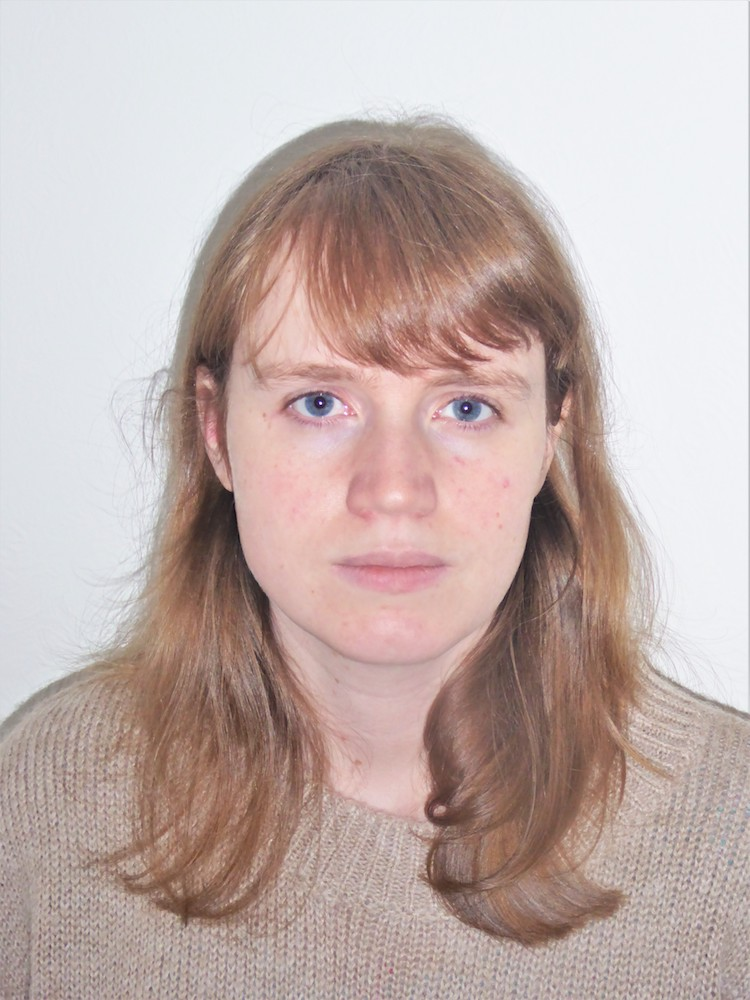
\includegraphics[width=0.2\textwidth]{1-introduction/img/natalie-lawton.jpg} & \textbf{Natalie Lawton - Management and Electrical Division}

\smallskip
\textit{Current Education}: MSc in Spacecraft Design.

\smallskip
\textit{Previous Education}: MEng in Aerospace Engineering. Previous experience in UAV avionic systems and emissions measurement techniques.

\smallskip
\textit{Responsibilities}: Acting as  Systems Engineer/Project Manager from the CDR until the end of the project. Previously was acting as deputy to these roles and in the electrical division. \DIFdelbegin \DIFdel{Ensures testing is }\DIFdelend \DIFaddbegin \DIFadd{Ensured testing was }\DIFaddend planned and executed. \DIFdelbegin \DIFdel{Oversees }\DIFdelend \DIFaddbegin \DIFadd{Oversaw }\DIFaddend manufacture, maintaining coordination between different teams and preventing project creep. Coordinating between different teams, project stakeholders, and documentation efforts. 
\bigskip
\\

 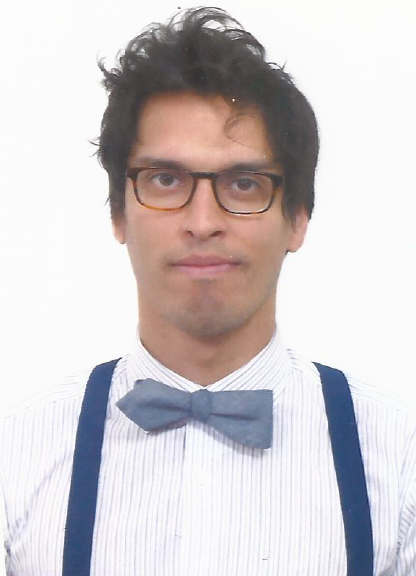
\includegraphics[width=0.2\textwidth]{1-introduction/img/georges-louis-joseph-labreche.jpg}  & \textbf{Georges L. J. Labrèche - Management Division}

\smallskip
\textit{Current Education}: MSc in Spacecraft Design.

\smallskip
\textit{Previous Education}: BSc in Software Engineering with experience in technical leadership and project management in software development.

\smallskip
\textit{Responsibilities}: Acting as Systems Engineer / Project Manager and managing overall implementation of the project until the Critical Design Review (CDR). Establishing and overseeing product development cycle. Coordinating between different teams, project stakeholders, and documentation efforts.                          
\bigskip
\\

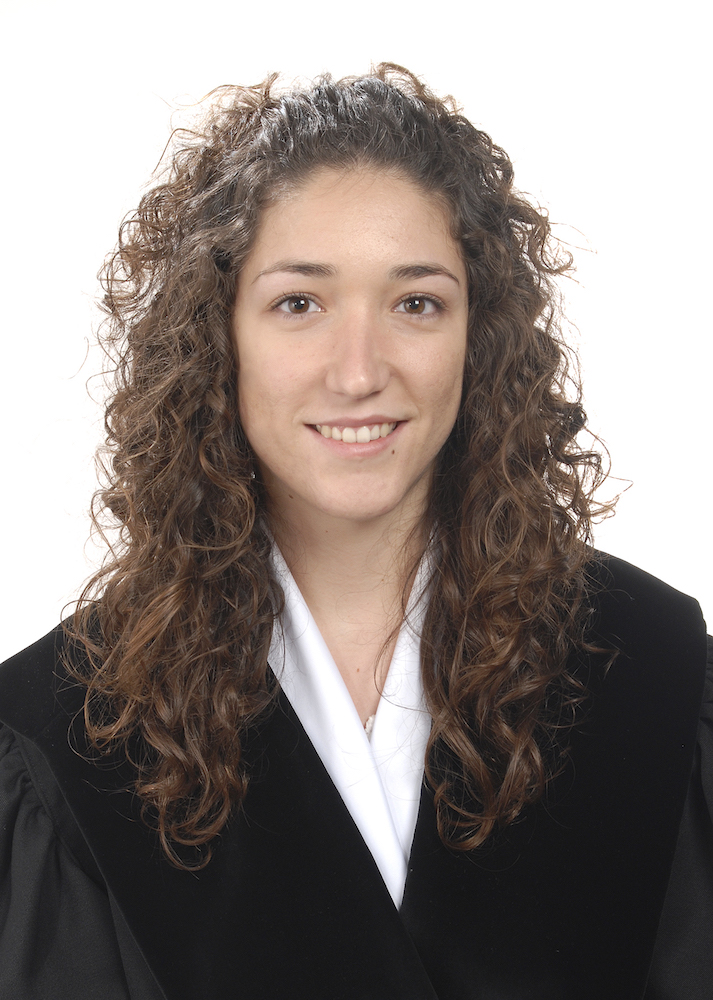
\includegraphics[width=0.2\textwidth]{1-introduction/img/agues-paszkowsky.jpg} & \textbf{Nuria Agües Paszkowsky - Scientific Division}

\smallskip
\textit{Current Education}: MSc in Earth Atmosphere and the Solar System.

\smallskip
\textit{Previous Education}: BSc in Aerospace Engineering.

\smallskip
\textit{Responsibilities}: Defining experiment parameters; data analysis; interpreting and documenting measurements; research on previous CAC experiments for comparative analysis purposes; contacting researchers or institutions working on similar projects; exploring potential partnership with researchers and institutions, evaluating the reliability of the proposed AAC sampling system; conducting measurements of collected samples; documenting and publishing findings. 
\bigskip
\\

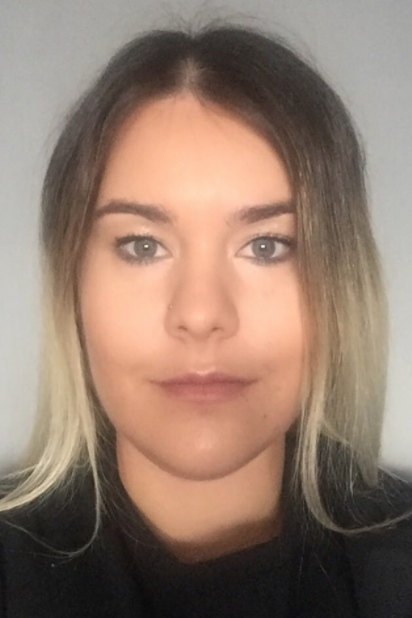
\includegraphics[width=0.2\textwidth]{1-introduction/img/kiki-blazaki.jpg} & \textbf{Kyriaki Blazaki - Scientific Division}

\smallskip
\textit{Current Education}: MSc in Earth Atmosphere and the Solar System.

\smallskip
\textit{Previous Education}: BSc in Physics.


\smallskip
\textit{Responsibilities}: Coordinating between the Scientific Division and the Project Manager; defining experiment parameters; data analysis; interpreting and documenting measurements; research on previous CAC experiments for comparative analysis purposes; evaluating the reliability of the proposed AAC sampling system; conducting measurements of collected samples; documenting and publishing findings. 
\bigskip
\\

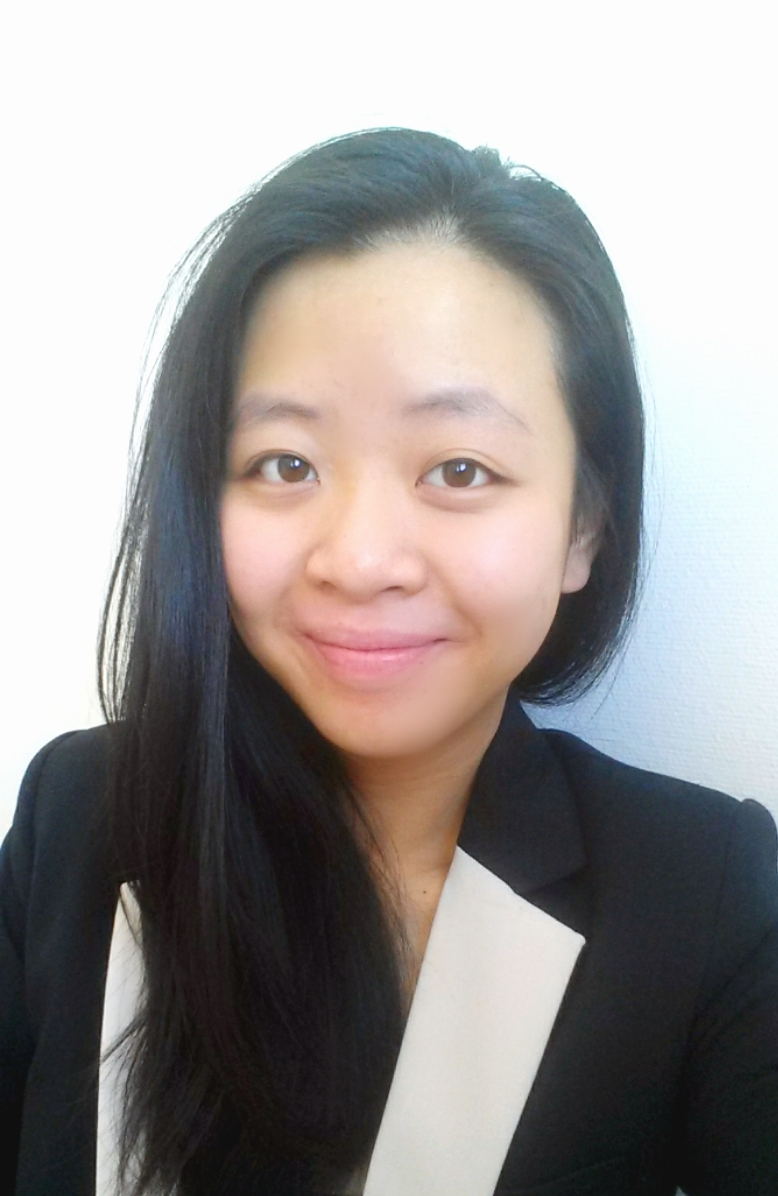
\includegraphics[width=0.2\textwidth]{1-introduction/img/emily-chen.jpeg} & \textbf{Emily Chen - Mechanical Division}

\smallskip
\textit{Current Education}: MSc in Space Engineering (5th Year).


\smallskip
\textit{Responsibilities}: Mechanical designing and assembly of CAC subsystem; analyzing the test results and changing the design as needed in collaboration with the team leader; integrating and assembling final design. 
\bigskip
\\

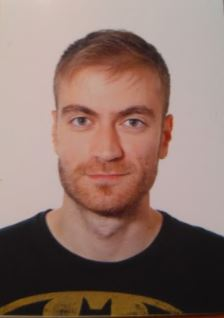
\includegraphics[width=0.2\textwidth]{1-introduction/img/jordi-coll-ortega.jpg} & \textbf{Jordi Coll Ortega - Mechanical Division}

\smallskip
\textit{Current Education}: MSc in Spacecraft Design.

\smallskip
\textit{Previous Education}: BASc in Aerospace Vehicle Engineering.

\smallskip
\textit{Responsibilities}: Designing or redesigning cost-effective mechanical devices using analysis and computer-aided design; developing and testing prototypes of designed devices; analyzing the test results and changing the design as needed in collaboration with the team lead; integrating and assembling final design.
\bigskip
\\

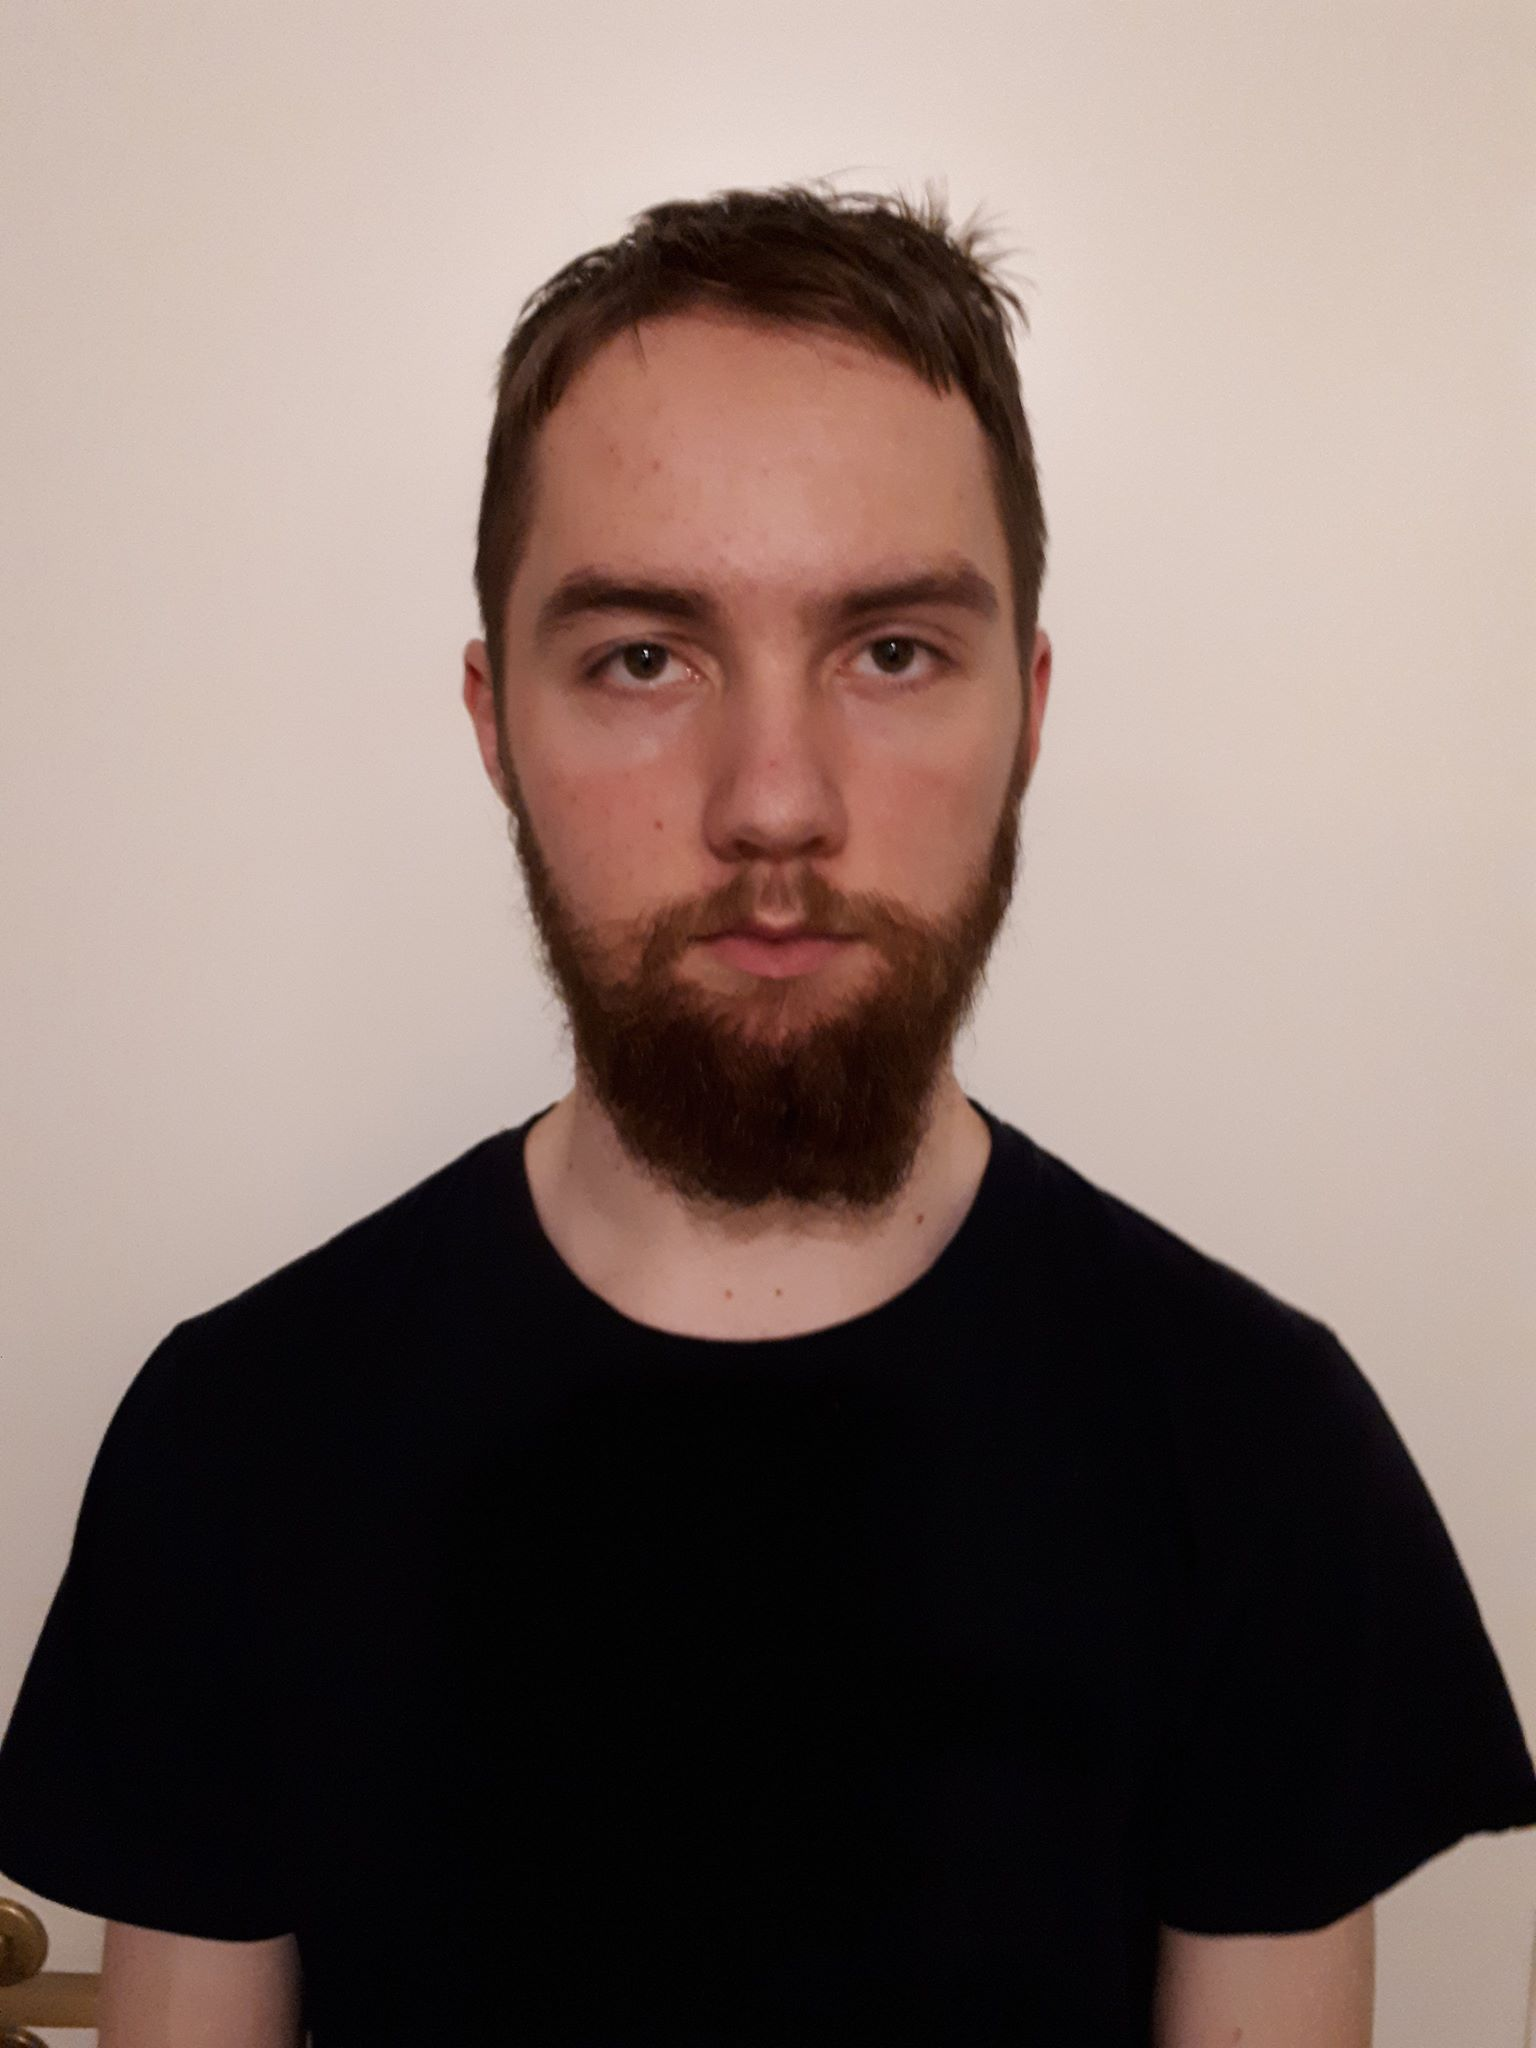
\includegraphics[width=0.2\textwidth]{1-introduction/img/gustav-dryssen.jpg} & \textbf{Gustav Dyrssen - Software Division}

\smallskip
\textit{Current Education}: MSc in Space Engineering (5th Year).

\smallskip
\textit{Responsibilities}: Leading quality assurance and testing efforts; Enforcing software testing best practices such as continuous integration testing and regression testing; reviewing requirements and specifications in order to foresee potential issues; provide input of functional requirements; advising on design; formalizing test cases; tracking defects and ensuring their resolution; facilitating code review sessions; supporting software implementation efforts.     
\bigskip
\\



\includegraphics[width=0.2\textwidth]{1-introduction/img/erik-fagerstrom.jpg} & \textbf{Erik Fagerström - Thermal Division}

\smallskip
\textit{Current Education}: MSc in Space Engineering (5th Year).


\smallskip
\textit{Responsibilities}: Coordinating between the Thermal Division and the Project Manager. Planning project thermal analysis and testing strategy. Thermal simulations of proposed designs and analyze results.
\bigskip
\\


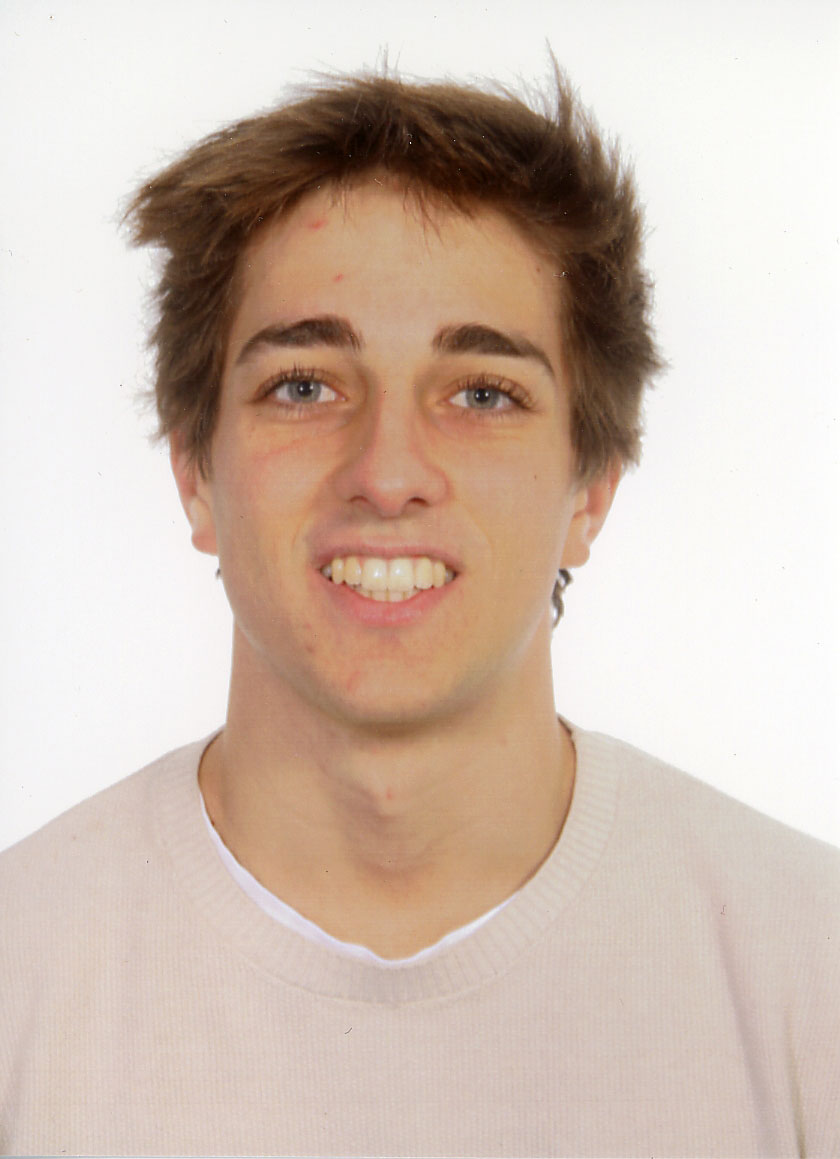
\includegraphics[width=0.2\textwidth]{1-introduction/img/pau-molas-roca.jpg} & \textbf{Pau Molas Roca - Mechanical Division}

\smallskip
\textit{Current Education}: MSc in Spacecraft Design.

\smallskip
\textit{Previous Education}: BSc in Aerospace Technology Engineering, Mechanical experience.

\smallskip
\textit{Responsibilities}: Coordinating between the Mechanical Division and the Project Manager; designing or redesigning cost-effective mechanical devices using analysis and computer-aided design; producing details of specifications and outline designs; overseeing the manufacturing process for the devices; identifying material and component suppliers; integrating and assembling final design.   \bigskip
\\


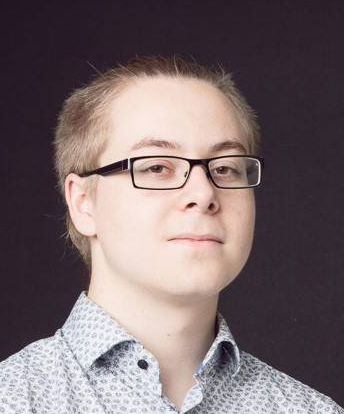
\includegraphics[width=0.2\textwidth]{1-introduction/img/emil-nordqvist.jpg} & \textbf{Emil Nordqvist - Electrical Division}

\smallskip
\textit{Current Education}: MSc in Space Engineering (5th Year).

\smallskip
\textit{Responsibilities}: Quality assurance of circuit design and implementation. Developing, testing, and evaluating theoretical designs.  \bigskip
\\

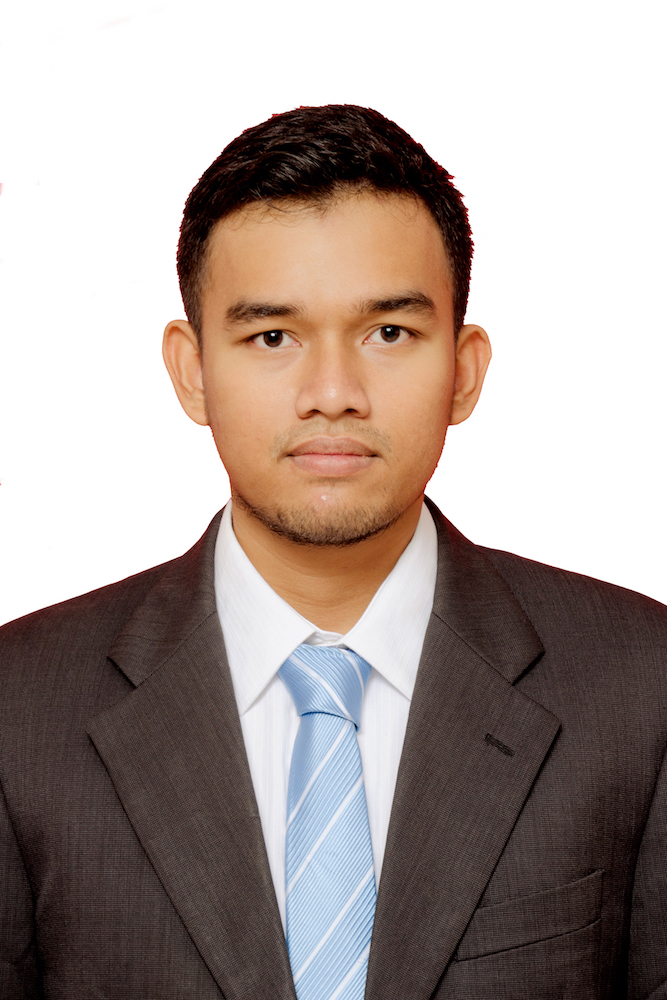
\includegraphics[width=0.2\textwidth]{1-introduction/img/muhammad-ansyar-rafi-putra.jpg} & \textbf{Muhammad Ansyar Rafi Putra - Software Division}

\smallskip
\textit{Current Education}: MSc in Spacecraft Design.

\smallskip
\textit{Previous Education}: BSc in Aerospace Engineering.


\smallskip 
\textit{Responsibilities}: Coordinating between the Software Division and the Project Manager; gathering software requirements; formalizing software specifications; drafting architecture design, detailed design; leading software implementation efforts.
\bigskip
\\

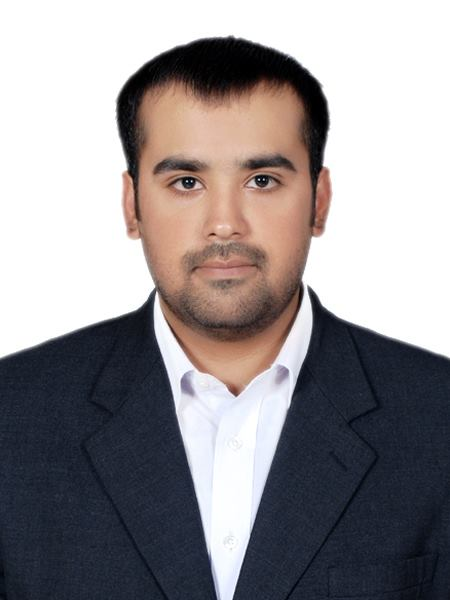
\includegraphics[width=0.2\textwidth]{1-introduction/img/hamad-saddiqi.jpg} & \textbf{Hamad Siddiqi - Electrical Division}


\smallskip
\textit{Current Education}: MSc Satellite Engineering.

\smallskip
\textit{Previous Education}: BSc in Electrical Engineering with experience in telecommunication industry and electronics.

\smallskip
\textit{Responsibilities}: Coordinating between the Electrical Division and the Project Manager; designing and implementing cost-effective circuitry using analysis and computer-aided design; producing details of specifications and outline designs; developing, testing, and evaluating theoretical designs; identifying material as well as component suppliers. 
\bigskip
\\


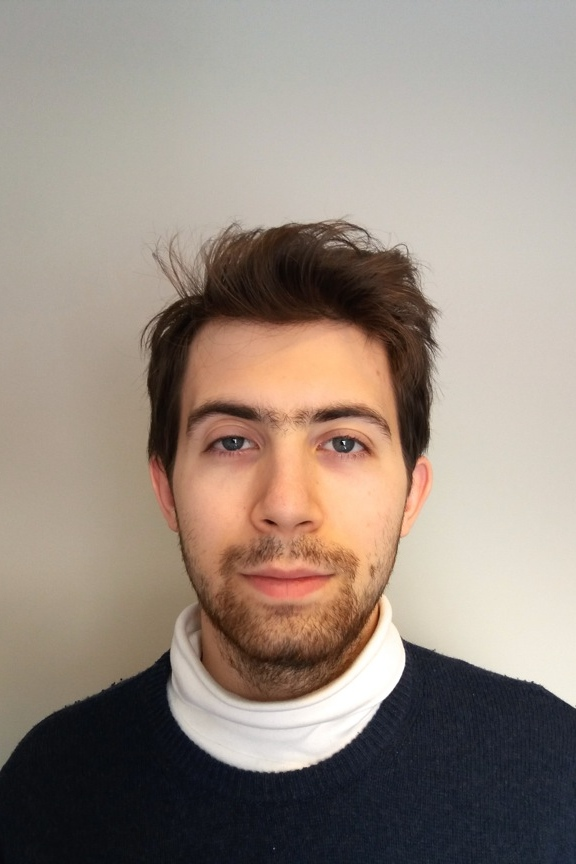
\includegraphics[width=0.2\textwidth]{1-introduction/img/ivan-zankov.jpg} & \textbf{Ivan Zankov - Thermal Division}

\smallskip
\textit{Current Education}: MSc in Spacecraft Design.

\smallskip
\textit{Previous Education}: BEng in Mechanical Engineering.

\smallskip
\textit{Responsibilities}: Thermal analysis of proposed designs and analysis result based recommendations.                                                         

\\
\label{tab:people}
\end{longtable}
\raggedbottom

\pagebreak
\section{Experiment Requirements and Constraints}
Requirements in this section does not list obsolete requirements. For a complete list of requirements that include obsolete ones, refer to Appendix \ref{sec:appFullListOfRequirements}.

\subsection{Functional Requirements}

\begin{enumerate}
    \item[F.2] The experiment \textit{shall} collect air samples by the CAC.
    \item[F.3] The experiment \textit{shall} collect air samples by the AAC.
    \item[F.9] The experiment \textit{should} measure the air intake flow to the AAC.
    \item[F.10] The experiment \textit{shall} measure the air pressure.
    \item[F.11] The experiment \textit{shall} measure the temperature.
\end{enumerate}
\subsection{Performance Requirements}

\begin{enumerate}
    %\item The programmable sampling rate of the pressure sensor \textit{shall} not be lesser than .
    \item[P.12] The accuracy of the ambient pressure measurements \textit{shall} be -1.5/+1.5 hPa for 25$\degree{C}$.
    \item[P.13] The accuracy of temperature measurements \textit{shall} be +3.5/-3$\degree{C}$ (max) for condition of -55$\degree{C}$ to 150$\degree{C}$.
    \item[P.23] The temperature sensor sampling rate \textit{shall} be 1 Hz.\label{newsamplerate}
    \item[P.24] The temperature of the Pump \textit{shall} be between 5$\degree{C}$ and 40$\degree{C}$. 
    \item[P.25] The minimum volume of air in the bags for analysis \textit{shall} be 0.18 L at ground level.
    \item[P.26] The equivalent flow rate of the pump \textit{shall} be between 8 to 3 L/min from ground level up to 24 km altitude.
    \item[P.27] The accuracy range of the sampling time, or the resolution, \textit{shall} be less than 52.94 s, or 423.53 m.
    \item[P.28] The pressure sensor sampling rate \textit{shall} be 1 Hz.\label{newsamplerate}
    \item[P.29] The airflow sensor sampling rate \textit{shall} be 1 Hz.\label{newsamplerate}
    \item[P.30] The accuracy of the pressure measurements inside the tubing and sampling bags \textit{shall} be -0.005/+0.005 bar for 25$\degree{C}$.

 \end{enumerate} 
\pagebreak
\subsection{Design Requirements}

\begin{enumerate}
    \item[D.1] The experiment \textit{shall} operate in the temperature profile of the BEXUS flight\cite{BexusManual}.
    \item[D.2] The experiment \textit{shall} operate in the vibration profile of the BEXUS flight\cite{BexusManual}.
    \item[D.3] The experiment \textit{shall} not have sharp edges or loose connections to the gondola that can harm the launch vehicle, other experiments, and people.%\textsuperscript{\ref{fn:unnecessary-requirement}}
    \item[D.4] The experiment's communication system \textit{shall} be compatible with the gondola's E-link system with the RJF21B connector over UDP for down-link and TCP for up-link.
    \item[D.5] The experiment's power supply \textit{shall} have a 24v, 12v, 5v and 3.3v power output and be able to take 28.8v input through the Amphenol PT02E8-4P connector supplied from the gondola. 
    \item[D.7] For the supplied voltage of 28.8 V, the total continuous DC current draw \textit{should} be below 1.8 A.
    \item[D.8] The total power consumption \textit{should} be below 374 Wh.
    \item[D.16] The experiment \textit{shall} be able to autonomously turn itself off just before landing.
    \item[D.17] The experiment box \textit{shall} be placed with at least one face exposed to the outside.
    \item[D.18] The experiment \textit{shall} operate in the pressure profile of the BEXUS flight\cite{BexusManual}.
    \item[D.19] The experiment \textit{shall} operate in the vertical and horizontal accelerations profile of the BEXUS flight\cite{BexusManual}.
    \item[D.21] The experiment \textit{shall} be attached to the gondola's rails.
    \item[D.22] The telecommand data rate \textit{shall} not be over 10 kb/s.
    \item[D.23] The air intake rate of the air pump \textit{shall} be equivalent to a minimum of 3 L/min at 24 km altitude.
    \item[D.24] The temperature of the Brain\footnote{The Brain is a central command unit which contains Electronic Box and pneumatic sampling system.} \textit{shall} be between -10$\degree{C}$ and 25$\degree{C}$.
    \item[D.26] The air sampling systems \textit{shall} filter out all water molecules before filling the sampling bags.
    \item[D.27] The total weight of the experiment \textit{shall} be less than 28 kg.
    \item[D.28] The AAC box \textit{shall} be able to fit at least $6$ air sampling bags.
    \item[D.29] The CAC box \textit{shall} take less than 3 minutes to be removed from the gondola without removing the whole experiment.
    \item[D.30] The AAC \textit{shall} be re-usable for future balloon flights.
    \item[D.31] The altitude from which a sampling bag will start sampling \textit{shall} be programmable.
    \item[D.32] The altitude from which a sampling bag will stop sampling \textit{shall} be programmable.
\end{enumerate}
\pagebreak
\pagebreak
\subsection{Operational Requirements}

\begin{enumerate}
    \item[O.13] The experiment \textit{should} function automatically.
    \item[O.14] The experiment's air sampling mechanisms \textit{shall} have a manual override.
\end{enumerate} 
\subsection{Constraints}

\begin{enumerate}
    \item[C.1] Constraints specified in the BEXUS User Manual.
\end{enumerate}



\pagebreak
\section{Project Planning}

\subsection{Work Breakdown Structure}

The team \DIFdelbegin \DIFdel{is }\DIFdelend \DIFaddbegin \DIFadd{was }\DIFaddend categorized into different groups of responsibilities with dedicated leaders who \DIFdelbegin \DIFdel{will report to and coordinate }\DIFdelend \DIFaddbegin \DIFadd{reported to and coordinated }\DIFaddend with the Project Manager. Leadership \DIFdelbegin \DIFdel{may be }\DIFdelend \DIFaddbegin \DIFadd{was }\DIFaddend organized on a rotational basis \DIFdelbegin \DIFdel{should the need arise}\DIFdelend \DIFaddbegin \DIFadd{when the need arose}\DIFaddend . The formation of these divisions \DIFdelbegin \DIFdel{constitute }\DIFdelend \DIFaddbegin \DIFadd{constituted }\DIFaddend a work breakdown structure \DIFdelbegin \DIFdel{in }\DIFdelend which is illustrated in Figure \ref{fig:work-breakdown-structure}.

The \DIFdelbegin \DIFdel{interaction between the divisions will be refined over the course of project implementation to acknowledge the interdisciplinary nature of the experiment around a Payload / Platform scheme.
}%DIFDELCMD < 

%DIFDELCMD < %%%
\DIFdel{The Management is }\DIFdelend \DIFaddbegin \DIFadd{Management was }\DIFaddend composed of a Project Manager and a Deputy Project Manager, both \DIFdelbegin \DIFdel{acting }\DIFdelend \DIFaddbegin \DIFadd{acted }\DIFaddend as Systems Engineer and \DIFdelbegin \DIFdel{managing }\DIFdelend \DIFaddbegin \DIFadd{managed the }\DIFaddend overall implementation of the project. The Project Manager \DIFdelbegin \DIFdel{is }\DIFdelend \DIFaddbegin \DIFadd{was }\DIFaddend responsible for establishing and overseeing product development cycle; coordinating between different teams, project stakeholders, and documentation efforts; outreach and public relations; Fundraising; monitoring and reporting; system integration; and quality assurance. Once all subsystems \DIFdelbegin \DIFdel{have }\DIFdelend \DIFaddbegin \DIFadd{had }\DIFaddend been assembled, the Project Manager \DIFdelbegin \DIFdel{will be }\DIFdelend \DIFaddbegin \DIFadd{was also }\DIFaddend responsible for overseeing the integration processes leading to the final experiment setup and \DIFdelbegin \DIFdel{will }\DIFdelend put emphasis on leading quality assurance integration testing efforts. The Deputy Project Manager \DIFdelbegin \DIFdel{assists }\DIFdelend \DIFaddbegin \DIFadd{assisted }\DIFaddend the Project Manager in all management duties in a manner that \DIFdelbegin \DIFdel{ensures }\DIFdelend \DIFaddbegin \DIFadd{ensured }\DIFaddend replaceability when necessary.

The Scientific Division \DIFdelbegin \DIFdel{is }\DIFdelend \DIFaddbegin \DIFadd{was }\DIFaddend responsible for defining experiment parameters; data analysis; interpreting and documenting measurements; researching previous CAC experiments for comparative analysis purposes; evaluating the reliability of the proposed AAC sampling system; conducting measurements of collected samples; documenting and publishing findings; defining experiment parameters; contacting researchers or institutions working on similar projects; exploring potential partnership with researchers and institutions; documenting and publishing findings.

The Mechanical Division \DIFdelbegin \DIFdel{is }\DIFdelend \DIFaddbegin \DIFadd{was }\DIFaddend responsible for designing or redesigning cost-effective mechanical devices using analysis and computer-aided design; producing details of specifications and outline designs; overseeing the manufacturing process for the devices; identifying material and component suppliers; developing and testing prototypes of designed devices; analyzing test results and changing the design as needed; and integrating and assembling final design.

The Electrical Division \DIFdelbegin \DIFdel{is }\DIFdelend \DIFaddbegin \DIFadd{was }\DIFaddend responsible for designing and implementing cost-effective circuitry using analysis and computer-aided design; producing details of specifications and outline designs; developing, testing, and evaluating theoretical designs; identifying material as well as component suppliers; reviewing and testing proposed designs; recommending modifications following prototype test results; and assembling designed circuitry.

The Software Division \DIFdelbegin \DIFdel{is }\DIFdelend \DIFaddbegin \DIFadd{was }\DIFaddend responsible for gathering software requirements; formalizing software specifications; drafting architecture design; leading software implementation efforts; leading quality assurance and testing efforts; enforcing software testing best practices such as continuous integration testing and regression testing; reviewing requirements and specifications in order to foresee potential issues; providing input for functional requirements; advising on design; formalizing test cases; tracking defects and ensuring their resolution; facilitating code review sessions; and supporting software implementation efforts.

The Thermal Division \DIFdelbegin \DIFdel{is }\DIFdelend \DIFaddbegin \DIFadd{was }\DIFaddend responsible for ensuring thermal regulation of the payload as per operational requirements of all experiment components; evaluating designs against thermal simulation and propose improvements; managing against mechanical design and electrical power limitations towards providing passive and active thermal control systems.

\begin{landscape}
\begin{figure}[p]
    \begin{align*}
        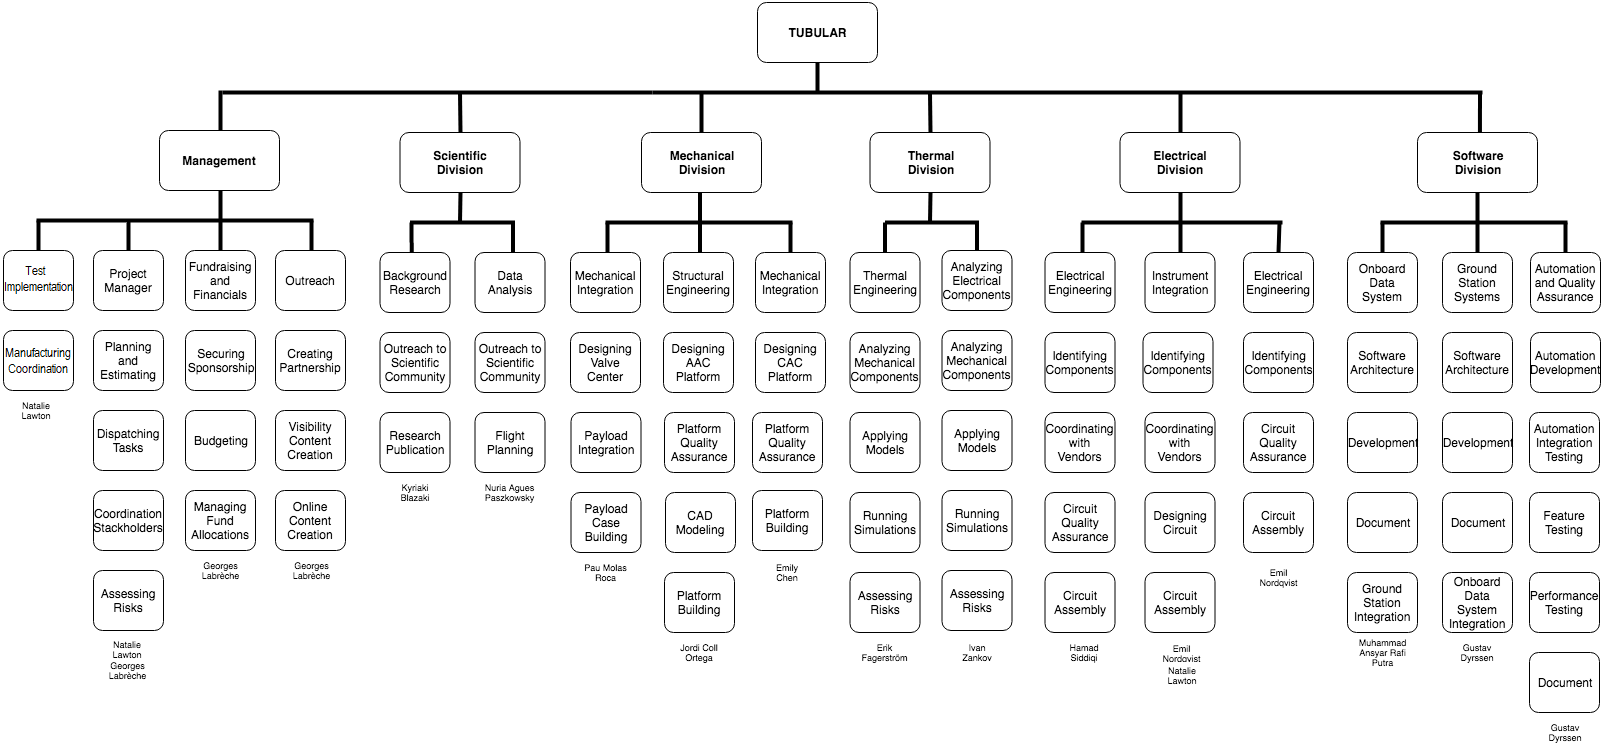
\includegraphics[width=24cm]{3-project-planning/img/work-breakdown-structure-updated.png}
    \end{align*}
    \caption{Work Breakdown Structure.}\label{fig:work-breakdown-structure}
\end{figure}
\end{landscape}
\pagebreak
\subsection{Schedule}

Scheduling of the project is presented in a Gantt Chart overview on Figure \ref{fig:schedule-gantt-chart}. Exam period constraints \DIFdelbegin \DIFdel{have been }\DIFdelend \DIFaddbegin \DIFadd{were }\DIFaddend included in order to evaluate risks in person-day allocations to project implementation. It \DIFdelbegin \DIFdel{is }\DIFdelend \DIFaddbegin \DIFadd{was }\DIFaddend expected during exam periods the team work output \DIFdelbegin \DIFdel{will }\DIFdelend \DIFaddbegin \DIFadd{would }\DIFaddend be lower than usual but project activities \DIFdelbegin \DIFdel{will continue, therefore time has been }\DIFdelend \DIFaddbegin \DIFadd{did continue, with time }\DIFaddend planned accordingly to accommodate this:

\begin{figure}[H]
    \begin{align*}
        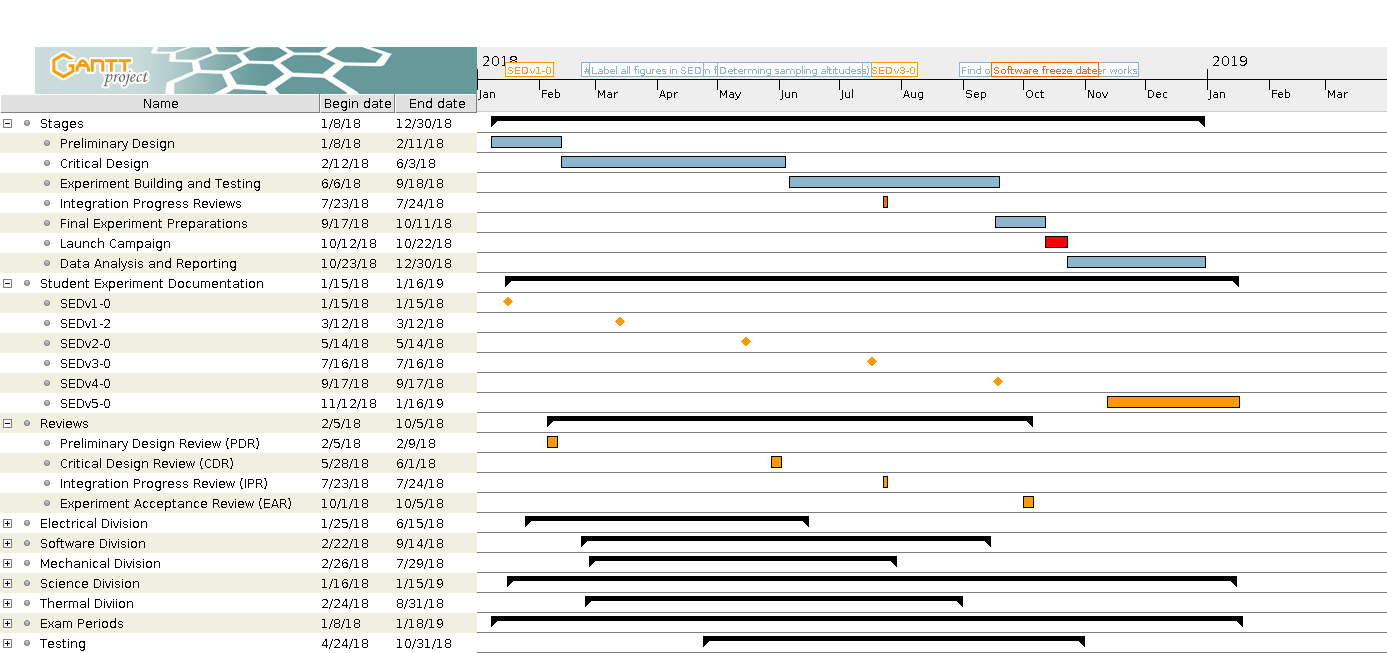
\includegraphics[width=1\linewidth]{3-project-planning/img/BEXUS-SED-GanttChart-Overview.png}
    \end{align*}
    \caption{Project Schedule Gantt Chart.}\label{fig:schedule-gantt-chart}
\end{figure}

\DIFdelbegin \DIFdel{Deadlines of the five Student Experiment Documentations (SED) versions have been estimated based on past REXUS/BEXUS Cycles. }\DIFdelend An expanded version of the Gantt Chart with detailed listing of all sub-tasks not shown in Figure \ref{fig:schedule-gantt-chart} can be found in Appendix \ref{sec:appF}. This expanded Gantt Chart includes all tasks related to the test plan and internal deadlines \DIFdelbegin \DIFdel{are }\DIFdelend \DIFaddbegin \DIFadd{were }\DIFaddend set so that a first draft of the documentation \DIFdelbegin \DIFdel{is }\DIFdelend \DIFaddbegin \DIFadd{was }\DIFaddend completed one week in advance to allow contents to be checked. Build and test internal deadlines \DIFdelbegin \DIFdel{are }\DIFdelend \DIFaddbegin \DIFadd{were }\DIFaddend also placed one week in advance to allow a buffer in case things \DIFdelbegin \DIFdel{do }\DIFdelend \DIFaddbegin \DIFadd{did }\DIFaddend not go as expected. The tests \DIFdelbegin \DIFdel{are }\DIFdelend \DIFaddbegin \DIFadd{were }\DIFaddend scheduled for as early as possible to allow time for rescheduling if the result \DIFdelbegin \DIFdel{is }\DIFdelend \DIFaddbegin \DIFadd{was }\DIFaddend a fail. With some high priority tests, see Section \ref{sec:5.2.1-testpriority}, it \DIFdelbegin \DIFdel{is expected these will }\DIFdelend \DIFaddbegin \DIFadd{was expected these would }\DIFaddend be very difficult to reschedule therefore extra time \DIFdelbegin \DIFdel{is }\DIFdelend \DIFaddbegin \DIFadd{was }\DIFaddend built into the test duration to allow for multiple attempts at the test.


\pagebreak
\subsection{Resources}

\subsubsection{Manpower}
The TUBULAR Team is categorized into divisions as summarized in Table \ref{tab:divisions-members}:

\begin{table}[H]
\centering
\resizebox{\textwidth}{!}{%
\begin{tabular}{|l|l|l|l|l|l|}
\hline
\textbf{Management} & \textbf{Scientific}    & \textbf{Mechanical} & \textbf{Electrical} & \textbf{Thermal} & \textbf{Software}          \\ \hline
Natalie Lawton*    & Kyriaki Blazaki*        & Pau Molas Roca*      & Hamad Siddiqi*  & Erik Fragerström*    & Muhammad Ansyar Rafi Putra* \\ \hline
Georges L. J. Labrèche & Nuria Agues Paszkowsky & Jordi Coll Ortega   & Emil Nordqvist  & Ivan Zankov  & Gustav Dyrssen             \\ \hline
 & & Emily Chen  &   &  &              \\ \hline
\end{tabular}%
}
\caption{Project Divisions and Members (Asterisks Denote Division Leaders).}
\label{tab:divisions-members}
\end{table}
\raggedbottom

The experience of TUBULAR Team members are listed in Table \ref{tab:team-member-experience}:

% Please add the following required packages to your document preamble:
% \usepackage{graphicx}
\begin{table}[H]
\centering
\begin{tabular}{|l|m{11cm}|}
\hline
\textbf{Team Member} & \textbf{Project Related Experience} \\ \hline
Natalie Lawton & MSc in Spacecraft Design (2nd Year). \\& MEng in Aerospace Engineering.\\& Previous experience in UAV avionic systems and emissions measurement techniques. \\ \hline
Nuria Agues Paszkowsky & MSc in Earth Atmosphere and the Solar System (2nd Year). \\& BSc in Aerospace Engineering.\\ \hline
Kyriaki Blazaki & MSc in Earth Atmosphere and the Solar System (2nd Year). \\& BSc in Physics. \\ \hline
Emily Chen & MSc in Space Engineering (5th Year). \\ \hline
Jordi Coll Ortega & MSc in Spacecraft Design (2nd Year). \\& BSc in Aerospace Vehicle Engineering. \\ \hline
Gustav Dyrssen &  MSc in Space Engineering (5th Year).\\ \hline
Erik Fagerström & MSc in Space Engineering (5th Year). \\ \hline
Georges L. J. Labrèche & MSc in Spacecraft Design (2nd Year). \\& BSc in Software Engineering.\\ \hline
Muhammad Ansyar Rafi Putra & MSc in Spacecraft Design (2nd Year). \\& BSc in Aerospace Engineering. \\ \hline
Pau Molas Roca & MSc in Spacecraft Design (2nd Year). \\& BSc in Aerospace Technology Engineering, Mechanical experience. \\ \hline
Emil Nordqvist & MSc in Space Engineering (5th Year). \\ \hline
Hamad Siddiqi & MSc Satellite Engineering (4th Year) \\&  BSc in Electrical Engineering.\\& Experience in telecommunication industry and electronics.  \\ \hline
Ivan Zankov & MSc in Spacecraft Design (2nd Year). \\& BEng in Mechanical Engineering.\\ \hline
\end{tabular}
\caption{Project Related Experience of Team Members.}
\label{tab:team-member-experience}
\end{table}
\raggedbottom

The initial projected effort to be contributed by each team member was averaged at 1.5 hour per person per day corresponding to a team total of 15 hours per day. Since then, 3 new members \DIFdelbegin \DIFdel{have }\DIFdelend \DIFaddbegin \DIFadd{had }\DIFaddend been included in the team thus increasing the projected daily effort to 19.5 hours per day. During the \DIFdelbegin \DIFdel{period leading up to the launch it is expected that the effort contributed will be double to 3 hours per person per day}\DIFdelend \DIFaddbegin \DIFadd{summer period many team members were away which meant that the team hours put in had little significant overall change}\DIFaddend . The period of these different effort capacities are listed in Table \ref{tab:daily-team-effort-per-period}:

\begin{table}[H]
\centering
\begin{tabular}{|c|c|c|}
\hline
\textbf{From} & \textbf{To} & \textbf{Capacity (hours/day)} \\ \hline
08/01/2018 & 18/03/2018 & 15 \\ \hline
19/03/2018 & 08/04/2018 & 16.5 \\ \hline
09/04/2018 & 09/05/2018 & 18 \\ \hline
10/05/2018 & 15/08/2018 & 19.5 \\ \hline
15/08/2018 & 22/10/2018 & \DIFdelbeginFL \DIFdelFL{39 }\DIFdelendFL \DIFaddbeginFL \DIFaddFL{19.5 }\DIFaddendFL \\ \hline
23/10/2018 & 31/01/2019 & 19.5 \\ \hline
\end{tabular}
\caption{Projected Daily Team Effort per Period.}
\label{tab:daily-team-effort-per-period}
\end{table}

Taking into account all team members and the mid-project changes in team size, the efforts/capacity projected to be allocated to each stages of the project during 2018 are summarized in Table \ref{tab:effort-allocation-stages}:

\begin{table}[H]
\centering
\begin{tabular}{lcc|c|c|c|c|}
\hline
\multicolumn{1}{|c|}{\multirow{2}{*}{\textbf{Stage}}} & \multicolumn{1}{c|}{\multirow{2}{*}{\textbf{\begin{tabular}[c]{@{}c@{}}Start\\ Date\end{tabular}}}} & \multirow{2}{*}{\textbf{\begin{tabular}[c]{@{}c@{}}End\\ Date\end{tabular}}} & \multirow{2}{*}{\textbf{\begin{tabular}[c]{@{}c@{}}Duration\\ (days)\end{tabular}}} & \multicolumn{3}{c|}{\textbf{Effort (hours)}} \\ \cline{5-7} 
\multicolumn{1}{|c|}{} & \multicolumn{1}{c|}{} &  &  & \textbf{Capacity} & \textbf{Actual} & \multicolumn{1}{l|}{\textbf{Diff. (\%)}} \\ \hline
\multicolumn{1}{|l|}{Preliminary Design} & \multicolumn{1}{c|}{08/01} & 11/02 & 35 & 525 & 708 & +29.68 \\ \hline
\multicolumn{1}{|l|}{Critical Design} & \multicolumn{1}{c|}{12/02} & 03/06 & 112 & 1,680 & 2,649 & +57.66 \\ \hline
\multicolumn{1}{|l|}{Experiment Building and Testing} & \multicolumn{1}{c|}{04/06} & 16/09 & 105 & \DIFdelbeginFL \DIFdelFL{3,072 }\DIFdelendFL \DIFaddbeginFL \DIFaddFL{2,048 }\DIFaddendFL & 1,943 & \DIFdelbeginFL \DIFdelFL{-36.76 }\DIFdelendFL \DIFaddbeginFL \DIFaddFL{-5.40 }\DIFaddendFL \\ \hline
\multicolumn{1}{|l|}{Final Experiment Preparations} & \multicolumn{1}{c|}{17/09} & 11/10 & 25 & \DIFdelbeginFL \DIFdelFL{976 }\DIFdelendFL \DIFaddbeginFL \DIFaddFL{488 }\DIFaddendFL & \DIFdelbeginFL \DIFdelFL{571* }\DIFdelendFL \DIFaddbeginFL \DIFaddFL{571 }\DIFaddendFL & \DIFdelbeginFL \DIFdelFL{-41.55* }\DIFdelendFL \DIFaddbeginFL \DIFaddFL{+17.00 }\DIFaddendFL \\ \hline
\multicolumn{1}{|l|}{Launch Campaign} & \multicolumn{1}{c|}{12/10} & 22/10 & 10 & 390 & \DIFdelbeginFL \DIFdelFL{- }\DIFdelendFL \DIFaddbeginFL \DIFaddFL{777 }\DIFaddendFL & \DIFdelbeginFL \DIFdelFL{- }\DIFdelendFL \DIFaddbeginFL \DIFaddFL{+99.23 }\DIFaddendFL \\ \hline
\multicolumn{1}{|l|}{Data Analysis and Reporting} & \multicolumn{1}{c|}{23/10} & 30/01 & 69 & 1,346 & \DIFdelbeginFL \DIFdelFL{- }\DIFdelendFL \DIFaddbeginFL \DIFaddFL{245 }\DIFaddendFL & \DIFdelbeginFL \DIFdelFL{- }\DIFdelendFL \DIFaddbeginFL \DIFaddFL{-81.78 }\DIFaddendFL \\ \hline
\multicolumn{1}{r}{\textbf{}} & \multicolumn{1}{l}{} & \multicolumn{1}{r|}{\textbf{Total:}} & \textbf{356} & \textbf{7,989} & \textit{\DIFdelbeginFL \DIFdelFL{5871*}\DIFdelendFL \DIFaddbeginFL \DIFaddFL{6939}\DIFaddendFL } & \textit{\DIFdelbeginFL \DIFdelFL{-26.51*}\DIFdelendFL \DIFaddbeginFL \DIFaddFL{-13.14}\DIFaddendFL } \\ \cline{4-7} 
\end{tabular}
\caption{Project Effort Allocation per Project Stages\DIFdelbeginFL \DIFdelFL{(Asterisks Denote Still Ongoing Stages)}\DIFdelendFL .}
\label{tab:effort-allocation-stages}
\end{table}

\DIFaddbegin \DIFadd{It can be seen that it was necessary at some stages to work more than was projected and at other stages less work was required to achieve the aims.
}

\DIFaddend All TUBULAR Team members are based in Kiruna, Sweden, just \SI{40}{\kilo\meter} from Esrange Space Center. Furthermore, all team members are enrolled in LTU Master programmes in Kiruna and thus \DIFdelbegin \DIFdel{expected to remain }\DIFdelend \DIFaddbegin \DIFadd{remained }\DIFaddend in LTU during the entire project period. Special attention \DIFdelbegin \DIFdel{will have to be }\DIFdelend \DIFaddbegin \DIFadd{was }\DIFaddend made for planning tasks during the summer period where many team members \DIFdelbegin \DIFdel{are expected to travel }\DIFdelend \DIFaddbegin \DIFadd{traveled }\DIFaddend abroad. A timeline of team member availability  until January 2019 is available in Appendix \ref{sec:appD}. A significant risk \DIFdelbegin \DIFdel{can be }\DIFdelend \DIFaddbegin \DIFadd{was }\DIFaddend observed during the summer months from June to August where most members \DIFdelbegin \DIFdel{will only be }\DIFdelend \DIFaddbegin \DIFadd{were only }\DIFaddend partially available and some completely unavailable. As such, team member availability and work commitments over the summer \DIFdelbegin \DIFdel{have been }\DIFdelend \DIFaddbegin \DIFadd{were }\DIFaddend negotiated across team members in order to guarantee that at least one member per division \DIFdelbegin \DIFdel{is }\DIFdelend \DIFaddbegin \DIFadd{was }\DIFaddend present in Kiruna over the Summer with the exception of the Software Division which \DIFdelbegin \DIFdel{can }\DIFdelend \DIFaddbegin \DIFadd{could }\DIFaddend work remotely. Furthermore, the Project Manager role \DIFdelbegin \DIFdel{will have to be }\DIFdelend \DIFaddbegin \DIFadd{was }\DIFaddend assigned to the Deputy Project Manager due to an extended full time unavailability after the CDR.

As part of their respective Master programmes, most TUBULAR Team members are enrolled in a project course at LTU. The TUBULAR project acts as the course's project for most team members from which they will obtain ECTS credits. This course is supervised by Dr. Thomas Kuhn, Associate Professor at LTU.

\pagebreak
\subsubsection{Budget}
\label{sec:3.2.2}
The experiment \DIFdelbegin \DIFdel{has }\DIFdelend \DIFaddbegin \DIFadd{had }\DIFaddend a total mass of \SI{24}{\kilo\gram} at a cost of 33,211 EUR. An error margin \DIFdelbegin \DIFdel{is }\DIFdelend \DIFaddbegin \DIFadd{was }\DIFaddend included in the budget corresponding to 10\% of the total costs of components to be purchased. A complete budget is available in Appendix \ref{sec:appO} and a detailed component mass and cost breakdown is available in Section \ref{sec:experiment-components} Experiment Components. This breakdown does not include spare components accounted for in the total costs. Dimensions and mass of the experiment are summarized in Table \ref{table:experiment-summary} in Section \ref{sec:mechanical-design} and Table \ref{tab:dim-mass-tab} in Section \ref{sec:dim-mass}. A contingency fund of 900 EUR \DIFdelbegin \DIFdel{is }\DIFdelend \DIFaddbegin \DIFadd{was }\DIFaddend allocated for unseen events such as component failures. Component loan and donations from sponsors account for 85\% of the project's total cost. LTU and SNSB funding accounts for the remaining 15\%. 

%
\begin{table}[H]
\centering
\begin{tabular}{|c|d{2}|d{2}|}%{D{.}{.}{1}}
\hline

\textbf{Category} & \textbf{Total Mass [g]} & \textbf{Total Price [EUR]} \\ \hline
Structure & 11,337.84 & 619.24 \\ \hline
Electronics Box & 510.50 & 1062.74 \\ \hline
Cables and Sensors & 1,200.62 & 586.20 \\ \hline
CAC & 5,539.00 & 23,114.00 \\ \hline
AAC & 3,541.00 & 4,444.71 \\ \hline
Tools & - & 332.53 \\ \hline
Travel & - & 500.00 \\ \hline
Contingency & - & 1000.00 \\ \hline
Shipping Costs and Error Margin & 2,212.90 & 568.17 \\ \hline
{\textbf{Total}} & \textbf{24,341.85} & \textbf{31,227.58} \\ \hline
\end{tabular}
\caption{Mass and Cost Budget.}
\label{table:mass-and-cost-budget}
\end{table}

\raggedbottom

The project \DIFdelbegin \DIFdel{benefits }\DIFdelend \DIFaddbegin \DIFadd{benefited }\DIFaddend from component donations from Restek, SMC Pneumatics, Teknolab Sorbent, KNF, Eurocircuits, and Lagers Masking Consulting as well as component loans from FMI. Furthermore, discounts were offered by Teknolab Sorbent and Bosch Rexroth. Euro value allocation of these sponsorships are presented in Table \ref{table:sponsroship-allocation}.

\begin{table}[H]
\centering
\begin{tabular}{l|m{0.12\textwidth}|l|r|r|r|c}
\hline
\multicolumn{1}{|l|}{\textbf{Sponsor}} & \multicolumn{1}{|c|}{\textbf{Type}} & \multicolumn{1}{c|}{\textbf{Value}} & \multicolumn{1}{c|}{\textbf{Allocated}} & \multicolumn{1}{c|}{\textbf{Unallocated}} & \multicolumn{1}{c|}{\textbf{\% Allocation}} & \multicolumn{1}{c|}{\textbf{Status}} \\ \hline
\multicolumn{1}{|l|}{LTU} & Funds & 2,500.00 & 2,301.57 & 1,874.62 & 75 & \multicolumn{1}{c|}{Received} \\ \hline
\multicolumn{1}{|l|}{SNSB} & Funds & 2,909.80 & 2,634.40 & 275.40 & 91 & \multicolumn{1}{c|}{Received} \\ \hline
\multicolumn{1}{|l|}{FMI} & Component loan & 22,561.45 & 22,561.45 & 0.00 & 100 & \DIFdelbeginFL %DIFDELCMD < \multicolumn{1}{c|}{Confirmed} %%%
\DIFdelendFL \DIFaddbeginFL \multicolumn{1}{c|}{Received} \DIFaddendFL \\ \hline
\multicolumn{1}{|l|}{Restek} & Component donation & 1,120.00 & 1,120.00 & 0.00 & 100 & \multicolumn{1}{c|}{Received} \\ \hline
\multicolumn{1}{|l|}{Teknolab} & Component donation & 380.00 & 380.00 & 0.00 & 100 & \multicolumn{1}{c|}{Received} \\ \hline
\multicolumn{1}{|l|}{SMC} & Component donation & 860.00 & 860.00 & 0.00 & 100 & \multicolumn{1}{c|}{Received} \\ \hline
\multicolumn{1}{|l|}{Lagers Maskin} & Component donation & 300.00 & 300.00 & 0.00 & 100 & \multicolumn{1}{c|}{Received} \\ \hline
\multicolumn{1}{|l|}{Swagelok} & Component donation & 1,863.82 & 1,863.82 & 0.00 & 100 & \multicolumn{1}{c|}{Received} \\ \hline
\multicolumn{1}{|l|}{KNF} & Component loan & 350.00 & 350.00 & 0.00 & 100 & \multicolumn{1}{c|}{Received} \\ \hline
\multicolumn{1}{|l|}{SilcoTek} & Component donation & 840.00 & 840.00 & 0.00 & 100 & \multicolumn{1}{c|}{Received} \\ \hline
\multicolumn{1}{|l|}{Eurocircuits} & Component donation & 426.95 & 426.95 & 0.00 & 100 & \multicolumn{1}{c|}{Received} \\ \hline
 & \multicolumn{1}{l|}{\textbf{Total}} & \textbf{34,112.01} & \textbf{33,211.24} & \textbf{900.77} & \textbf{97} & \multicolumn{1}{l}{} \\ \cline{2-6}
\end{tabular}
\caption{Allocation of Sponsorship Funds and Component Donation Values. Amounts in EUR.}
\label{table:sponsroship-allocation}
\end{table} 


\subsubsection{External Support}

Partnership with FMI, and IRF \DIFdelbegin \DIFdel{will provide }\DIFdelend \DIFaddbegin \DIFadd{has provided }\DIFaddend the team with technical guidance in implementing the sampling system. FMI’s experience in implementing past CAC sample systems provide invaluable lessons learned towards conceptualizing, designing, and implementing the proposed AAC sampling system.

\DIFdelbegin \DIFdel{FMI is }\DIFdelend \DIFaddbegin \DIFadd{FM Iwas }\DIFaddend a key partner in the TUBULAR project, its scientific experts \DIFdelbegin \DIFdel{will advise and support }\DIFdelend \DIFaddbegin \DIFadd{have advised and supported }\DIFaddend the TUBULAR project by sharing knowledge, experience, and granting accessibility of equipment. As per the agreement shown in Appendix \ref{sec:appG}, FMI \DIFdelbegin \DIFdel{will provide }\DIFdelend \DIFaddbegin \DIFadd{had provided }\DIFaddend the TUBULAR Team with the AirCore stainless tube component of the CAC subsystem as well as the post-flight gas analyzer. This arrangement \DIFdelbegin \DIFdel{requires }\DIFdelend \DIFaddbegin \DIFadd{required }\DIFaddend careful considerations on the placement of the experiment in order to minimize hardware damage risks. These contributions \DIFdelbegin \DIFdel{result }\DIFdelend \DIFaddbegin \DIFadd{resulted }\DIFaddend in significant cost savings regarding equipment and component procurement.

Daily access to LTU's Space Campus in Kiruna \DIFdelbegin \DIFdel{exposes }\DIFdelend \DIFaddbegin \DIFadd{exposed }\DIFaddend the team to scientific mentorship and expert guidance from both professors and researchers involved in the study of greenhouse gases and climate change. Dr Uwe Raffalski, IRF, Associate professor (Docent) \DIFdelbegin \DIFdel{is }\DIFdelend \DIFaddbegin \DIFadd{was }\DIFaddend one of many researchers involved in climate study \DIFdelbegin \DIFdel{who is mentoring }\DIFdelend \DIFaddbegin \DIFadd{whom mentored }\DIFaddend the team.
\pagebreak

\subsection{Outreach Approach}

The experiment as well as the REXUS/BEXUS programme and its partners \DIFdelbegin \DIFdel{will }\DIFdelend \DIFaddbegin \DIFadd{has been }\DIFaddend be promoted through the following activities:

\begin{itemize}
\item Research paper \DIFdelbegin \DIFdel{published }\DIFdelend \DIFaddbegin \DIFadd{publication work }\DIFaddend in partnership with FMI detailing the sampling methodology, measurement result, analysis, and findings.
\item Collected data will be licensed as open data to be freely available to everyone to use and republish as they wish, without restrictions from copyright, patents or other mechanisms of control.
\item A website to summarize the experiment and provide regular updates. Backend web analytics included to gauge interest on the project through number of visitors and their origins (See Appendix \ref{sec:appE}).
\item Dedicated Facebook page used as publicly accessible logbook detailing challenges, progress, and status of the project. Open for comments and questions (See Figure \ref{fig:outreach-facebook} in Appendix \ref{sec:appE}).
\item Two Instagram accounts for short and frequent image and video focused updates. A primary Instagram account will be dedicated to project updates. A secondary account will reach out to a broader audience by focusing on space instruments in general and cross-reference TUBULAR related activities when relevant (See Figures \ref{fig:outreach-instagram}, \ref{fig:outreach-instagram-si-1}, and \ref{fig:outreach-instagram-si-2} in Appendix \ref{sec:appE}).
\item GitHub account to host all project software code under free and open source license (See Figure \ref{fig:outreach-github} in Appendix \ref{sec:appE}). Other REXUS/BEXUS teams \DIFdelbegin \DIFdel{will be }\DIFdelend \DIFaddbegin \DIFadd{were }\DIFaddend invited to host their code in this account\DIFdelbegin \DIFdel{in what will hopefully become a centralized GitHub account and code archive for present and future REXUS/BEXUS projects}\DIFdelend .
\item\DIFdelbegin \DIFdel{Reddit Ask Me Anything (AMA) thread to discuss the project with community of online enthusiasts.
}%DIFDELCMD < \item%%%
\item%DIFAUXCMD
\DIFdelend \enquote{Show and Tell} trips to local high schools and universities. Team members \DIFdelbegin \DIFdel{will be }\DIFdelend \DIFaddbegin \DIFadd{were }\DIFaddend responsible to organize such presentations through any of their travel opportunities abroad.
\item Articles and/or blogposts about the project in team members' alma mater websites.
\item In-booth presentation and poster display in the seminars or career events at different universities. 
\item A thoroughly documented and user-friendly manual on how to build replicate and launch CAC and AAC sampling systems will be produced and published.
\end{itemize}
\pagebreak
\subsection{Risk Register}
\textbf{Risk ID}
\begin{enumerate}[label={}]
    \item TC – Technical/Implementation 
    \item MS – Mission (operational performance) 
    \item SF – Safety 
    \item VE – Vehicle 
    \item PE – Personnel 
    \item EN – Environmental 
    \item OR - Outreach
    \item BG - Budget
\end{enumerate}

Adapt these to the experiment and add other categories. 
Consider risks to the experiment, to the vehicle and to personnel. 

\textbf{Probability (P)}
\begin{enumerate}[label=\Alph*]
    \item Minimum – Almost impossible to occur 
    \item Low – Small chance to occur 
    \item Medium – Reasonable chance to occur 
    \item High – Quite likely to occur 
    \item Maximum – Certain to occur, maybe more than once
\end{enumerate}

\textbf{Severity (S)}
\begin{enumerate}
    \item Negligible – Minimal or no impact 
    \item Significant – Leads to reduced experiment performance 
    \item Major – Leads to failure of subsystem or loss of flight data 
    \item Critical – Leads to experiment failure or creates minor health hazards 
    \item Catastrophic – Leads to termination of the REXUS/BEXUS programme, damage to the vehicle or injury to personnel 
\end{enumerate}

The rankings for probability (P) and severity (S) \DIFdelbegin \DIFdel{are }\DIFdelend \DIFaddbegin \DIFadd{were }\DIFaddend combined to assess the overall risk classification, ranging from very low to very high and being coloured green, yellow, orange or red according to the SED guidelines.

\DIFdelbegin \DIFdel{Whether a risk is }\DIFdelend \DIFaddbegin \DIFadd{SED guidelines were used to determine whether a risk was }\DIFaddend acceptable or unacceptable\DIFdelbegin \DIFdel{has been assigned according to the SED guidelines. Where mitigation is written for acceptable risksthis details }\DIFdelend \DIFaddbegin \DIFadd{. For acceptable risks, details of }\DIFaddend the mitigation undertaken \DIFdelbegin \DIFdel{in order to reduce }\DIFdelend \DIFaddbegin \DIFadd{were included which reduced }\DIFaddend the risk to an acceptable level.

\begin{landscape}



\begin{longtable}{|m{0.075\textwidth}| m{0.48\textwidth} |m{0.02\textwidth} |m{0.02\textwidth}|m{0.10\textwidth}| m{0.64\textwidth}|}

\hline
\textbf{ID} & \textbf{Risk (\& consequence if)} & \textbf{P} & \textbf{S} & \textbf{P * S} & \textbf{Action} \\ \hline
TC10 & Software fails to store data & B & 2 & \cellcolor[HTML]{34FF34}Very Low & Acceptable Risk: Extensive testing \DIFdelbegin \DIFdel{will be }\DIFdelend \DIFaddbegin \DIFadd{has been }\DIFaddend done. Using telemetry, all data gathered from sensors will be sent to ground station. \\ \hline
TC20 & Failure of several sensors & B & 2 & \cellcolor[HTML]{34FF34}Very Low & Acceptable Risk: Thermal test (Test Number 5) \DIFdelbegin \DIFdel{to approve }\DIFdelend \DIFaddbegin \DIFadd{approved }\DIFaddend the functionality of the experiment. \\ \hline
TC30 & Critical component is destroyed in testing & B & 1 & \cellcolor[HTML]{34FF34}Very Low & Acceptable Risk: Spare components can be ordered but for expensive ones, they \DIFdelbegin \DIFdel{will be }\DIFdelend \DIFaddbegin \DIFadd{were }\DIFaddend ordered and tested early in the project in case we \DIFdelbegin \DIFdel{need }\DIFdelend \DIFaddbegin \DIFadd{needed }\DIFaddend to order more. \\ \hline
TC40 & Electrical connections dislodges or short circuits because of vibration or shock & B & 4 & \cellcolor[HTML]{FCFF2F}Low & Acceptable Risk. D-sub connections will be screwed in place. It \DIFdelbegin \DIFdel{will }\DIFdelend \DIFaddbegin \DIFadd{was }\DIFaddend be ensured that there \DIFdelbegin \DIFdel{are }\DIFdelend \DIFaddbegin \DIFadd{were }\DIFaddend no loose connections and zip ties \DIFdelbegin \DIFdel{will be }\DIFdelend \DIFaddbegin \DIFadd{were }\DIFaddend used to help keep wires in place. Careful soldering and extensive testing \DIFdelbegin \DIFdel{will be }\DIFdelend \DIFaddbegin \DIFadd{was }\DIFaddend applied. \\ \hline
TC50 & Experiment electronics fail due to long exposure to cold or warm temperatures & B & 3 & \cellcolor[HTML]{FCFF2F}Low & Acceptable Risk: Thermomechanical and thermoelectrical solutions \DIFdelbegin \DIFdel{will be }\DIFdelend \DIFaddbegin \DIFadd{were }\DIFaddend simulated and tested in detail to help prevent this from happening. \\ \hline
TC60 & Software and electrical fail to control heaters causing temperature to drop or rise below or above operational range & B & 2 & \cellcolor[HTML]{34FF34}Very Low & Acceptable Risk: Tests \DIFdelbegin \DIFdel{will be }\DIFdelend \DIFaddbegin \DIFadd{were }\DIFaddend performed prior to the flight to detect and minimize the risk of occurrence. The system \DIFdelbegin \DIFdel{will }\DIFdelend \DIFaddbegin \DIFadd{was }\DIFaddend be monitored during flight and handled manually if \DIFaddbegin \DIFadd{it was }\DIFaddend necessary. \\ \hline
TC70 & Software fails to enter safe mode (may result in loss of data) & B & 1 & \cellcolor[HTML]{34FF34}Very Low & Acceptable Risk: Extensive testing \DIFdelbegin \DIFdel{will }\DIFdelend \DIFaddbegin \DIFadd{was }\DIFaddend be done. \\ \hline
TC80 & On-board memory will be full (flight time longer than expected) & A & 2 & \cellcolor[HTML]{34FF34}Very Low & Acceptable Risk: The experiment \DIFdelbegin \DIFdel{shall go }\DIFdelend \DIFaddbegin \DIFadd{went }\DIFaddend through testing and analysis to guarantee the onboard memory size \DIFdelbegin \DIFdel{is }\DIFdelend \DIFaddbegin \DIFadd{was }\DIFaddend sufficient.\\ \hline
TC90 & Connection loss with ground station & A & 2 & \cellcolor[HTML]{34FF34}Very Low & Acceptable Risk: Experiment \DIFdelbegin \DIFdel{will be }\DIFdelend \DIFaddbegin \DIFadd{was }\DIFaddend designed to operate autonomously. \\ \hline
TC100 & Software fails to control valves autonomously & B & 2 & \cellcolor[HTML]{34FF34}Very Low & Acceptable Risk: Extensive testing \DIFdelbegin \DIFdel{will be }\DIFdelend \DIFaddbegin \DIFadd{was }\DIFaddend done. Telecommand \DIFdelbegin \DIFdel{will }\DIFdelend \DIFaddbegin \DIFadd{could }\DIFaddend also be used to manually control the valves. \\ \hline
TC110 & Software fails to change modes autonomously & B & 2 & \cellcolor[HTML]{34FF34}Very Low & Acceptable Risk: Extensive testing \DIFdelbegin \DIFdel{will be }\DIFdelend \DIFaddbegin \DIFadd{was }\DIFaddend done. Telecommand \DIFdelbegin \DIFdel{will }\DIFdelend \DIFaddbegin \DIFadd{could }\DIFaddend also be used to manually change experiment modes. \\ \hline
TC120 & Complete software failure & B & 4 & \cellcolor[HTML]{FCFF2F}Low & Acceptable Risk: A long duration testing (bench test) \DIFdelbegin \DIFdel{will be }\DIFdelend \DIFaddbegin \DIFadd{was }\DIFaddend performed to catch the failures early. \\ \hline
TC130 & Failure of fast recovery system & B & 2 & \cellcolor[HTML]{34FF34}Very Low & Acceptable Risk: Clear and simple instructions \DIFdelbegin \DIFdel{will be }\DIFdelend \DIFaddbegin \DIFadd{were }\DIFaddend given to the recovery team. A test \DIFdelbegin \DIFdel{will take }\DIFdelend \DIFaddbegin \DIFadd{took }\DIFaddend place before launch to ensure someone unfamiliar with the experiment \DIFdelbegin \DIFdel{can }\DIFdelend \DIFaddbegin \DIFadd{could }\DIFaddend remove the CAC box. Test number: 12. \\ \hline
TC140 & The gas analyzer isn't correctly calibrated and returns inaccurate results & B & 3 & \cellcolor[HTML]{FCFF2F}Low & Acceptable Risk: \DIFdelbegin \DIFdel{Calibrate the gas analyzer }\DIFdelend \DIFaddbegin \DIFadd{Gas analyzer was calibrated }\DIFaddend before use.\\ \hline 
TC150 & Partnership with FMI does not materialize, resulting in loss of access to CAC coiled tube. & B & 2 & \cellcolor[HTML]{34FF34}Very Low & Acceptable Risk: Signed agreement has been obtained. AAC sample analysis results can be validated against available historical data from past FMI CAC flights. \\ \hline 
MS10 & Down link connection is lost prematurely & B & 2 & \cellcolor[HTML]{34FF34}Very Low & Acceptable Risk: Data \DIFdelbegin \DIFdel{will }\DIFdelend \DIFaddbegin \DIFadd{was }\DIFaddend also be saved on SD card. \\ \hline
MS20 & Condensation on experiment PCBs which could causes short circuits & A & 3 & \cellcolor[HTML]{34FF34}Very Low & Acceptable Risk: The Brain \DIFdelbegin \DIFdel{will be }\DIFdelend \DIFaddbegin \DIFadd{was }\DIFaddend sealed to prevent condensation. \\ \hline
MS30 & Temperature sensitive components that are essential to full the mission objective might be below their operating temperature. & C & 3 & \cellcolor[HTML]{FCFF2F}Low & Acceptable Risk: Safe mode to prevent the components to operate out of its operating temperature range. \\ \hline
MS40 & Experiment lands in water causing electronics failure & B & 1 & \cellcolor[HTML]{34FF34}Very Low & Acceptable Risk: \DIFdelbegin \DIFdel{Check if SD card needs waterproof shell or is waterproof in itself. Also, all }\DIFdelend \DIFaddbegin \DIFadd{All }\DIFaddend the necessary data \DIFdelbegin \DIFdel{will }\DIFdelend \DIFaddbegin \DIFadd{was }\DIFaddend be downloaded during the flight. \\ \hline
MS50 & Interference from other experiments and/or balloon & A & 2 & \cellcolor[HTML]{34FF34}Very Low & Acceptable Risk: no action. \\ \hline
MS60 & Balloon power failure & B & 2 & \cellcolor[HTML]{FCFF2F}Low & Acceptable Risk: Valves default state \DIFdelbegin \DIFdel{is }\DIFdelend \DIFaddbegin \DIFadd{was }\DIFaddend closed so if all power is lost valves \DIFdelbegin \DIFdel{will }\DIFdelend \DIFaddbegin \DIFadd{would }\DIFaddend automatically close preserving all samples collected up until that point. \\ \hline
MS70 & Sampling bags disconnect & B & 3 & \cellcolor[HTML]{FCFF2F}Low & Acceptable Risk: The affected bags could not collect samples. The connection between the spout of the bags and the T-union \DIFdelbegin \DIFdel{shall be }\DIFdelend \DIFaddbegin \DIFadd{was }\DIFaddend double checked before flight. The system has passed vibration testing with no disconnects. \\ \hline
MS71 & Sampling bags puncture & B & 3 & \cellcolor[HTML]{FCFF2F}Low & Acceptable Risk: The affected bags could not collect samples. Inner styrofoam walls have been choosen and no sharp edges \DIFdelbegin \DIFdel{will be }\DIFdelend \DIFaddbegin \DIFadd{were }\DIFaddend exposed to avoid puncture from external elements. \\ \hline
MS72 & Sampling bags' hold time is typically 48h & B & 2 & \cellcolor[HTML]{34FF34}Very Low & Acceptable risk: Validation studies have demonstrated acceptable stability for up to 48 hours.  \\ \hline
MS80 & Pump failure & B & 3 & \cellcolor[HTML]{FCFF2F}Low & Acceptable Risk: A pump was chosen based on a previous similar experiment. The pump has also been tested in a low pressure chamber down to 10hPa and has successfully turned on and filled a sampling bag. The CAC subsystem is not reliant on the pump therefore would still operate even in the event of pump failure. \\ \hline
MS90 & Intake pipe blocked by external element & C & 3 & \cellcolor[HTML]{FCFF2F}Low & Acceptable Risk: The bags would not be filled and thus the AAC system would fail. An air filter \DIFdelbegin \DIFdel{will be }\DIFdelend \DIFaddbegin \DIFadd{was }\DIFaddend placed in both intake and outlet of the pipe to prevent this. \\ \hline
MS100 & Expansion/Contraction of insulation & B & 2 &\cellcolor[HTML]{34FF34}Very Low & Acceptable Risk: The insulation selected has flown successfully on similar flights in the past. Test \DIFdelbegin \DIFdel{shall be }\DIFdelend \DIFaddbegin \DIFadd{was }\DIFaddend done to see how it reacts in a low pressure environment. \\ \hline
MS110 & Sampling bags are over-filled resulting in bursting and loss of collected samples. & B & 3 & \cellcolor[HTML]{FCFF2F}Low & Acceptable Risk: Test \DIFdelbegin \DIFdel{will be }\DIFdelend \DIFaddbegin \DIFadd{was }\DIFaddend performed at target ambient pressure levels to identify how long the pump needs to fill the sampling bags. A static pressure sensor on board \DIFdelbegin \DIFdel{will monitor }\DIFdelend \DIFaddbegin \DIFadd{monitored }\DIFaddend the in-bag pressure during sampling and no bag \DIFdelbegin \DIFdel{will }\DIFdelend \DIFaddbegin \DIFadd{would }\DIFaddend ever be over pressured. In addition an airflow rate sensor \DIFdelbegin \DIFdel{will monitor }\DIFdelend \DIFaddbegin \DIFadd{monitored }\DIFaddend the flow rate and a timer started when a bag valve is opened. The sampling \DIFdelbegin \DIFdel{will }\DIFdelend \DIFaddbegin \DIFadd{would }\DIFaddend stop when either the maximum allowed pressure or maximum allowed time is reached. \\ \hline
SF10 & Safety risk due to pressurized vessels during recovery. & A & 1 & \cellcolor[HTML]{34FF34}Very Low & Acceptable Risk: The volume of air in the AAC decreases during descent because the pressure inside is lower than outside. The CAC is sealed at nearly sea level pressure, therefore there is only a small pressure difference.  \\ \hline
SF20 & Safety risk due to the use of chemicals such as magnesium perchlorate. & A & 4 & \cellcolor[HTML]{34FF34}Very Low & Acceptable Risk: The magnesium perchlorate \DIFdelbegin \DIFdel{will }\DIFdelend \DIFaddbegin \DIFadd{was }\DIFaddend be kept in a sealed container or filter at all times. Magnesium perchlorate filters are made of stainless steel which has high durability, and have been used before without any sealing problems.  \\ \hline
VE10 & SD-card is destroyed at impact & B & 2 & \cellcolor[HTML]{34FF34}Very Low & Acceptable Risk: All data \DIFdelbegin \DIFdel{will }\DIFdelend \DIFaddbegin \DIFadd{was }\DIFaddend be transmitted to the ground. Most of the data is the gas stored in the AAC and CAC. \\ \hline
VE20 & Gondola Fixing Interface & B & 4 & \cellcolor[HTML]{FCFF2F}Low & Acceptable Risk: The experiment box could detach from the gondola’s rails and the two boxes could detach one from the other. The experiment will be secured to the gondola and to each other with multiple fixings. These \DIFdelbegin \DIFdel{will }\DIFdelend \DIFaddbegin \DIFadd{were }\DIFaddend also be tested. \\ \hline
VE30 & Structure damage due to bad landing & B & 3 & \cellcolor[HTML]{FCFF2F}Low & Acceptable Risk: Landing directly on a hard element could break the structure or the protective walls. Consistent design implemented to prevent it. \\ \hline
VE40 & Hard landing damages the CAC equipment & C & 3 & \cellcolor[HTML]{FCFF2F}Low & Acceptable Risk:  Structural analysis has been done and choosing a wall consisting of an aluminum sheet and Styrofoam to dampen the landing. \\ \hline
VE50 & Hard landing damages the AAC equipment & C & 3 & \cellcolor[HTML]{FCFF2F}Low & Acceptable Risk:  Structural analysis has been done and choosing a wall consisting of an aluminum sheet and Styrofoam to dampen the landing. \\ \hline
EN10 & Vibrations from pump affect samples & C & 1 & \cellcolor[HTML]{34FF34}Very Low & Acceptable Risk: Vibrations do not affect the sampled air. No action required. \\ \hline
EN20 & The air samples must be protected from direct sunlight and stored above 0$\degree{C}$ to prevent condensation & C & 3 & \cellcolor[HTML]{FCFF2F}Low & Acceptable Risk: Stratospheric air is generally dry and water vapor concentrations are higher closer to the surface. In addition magnesium perchlorate dryers \DIFdelbegin \DIFdel{will be used to minimizing }\DIFdelend \DIFaddbegin \DIFadd{were used to minimize }\DIFaddend the risk of condensation.    \\ \hline 
PE10 & Change in Project Manager after the CDR introduces a gap of knowledge in management responsibilities. & E & 1 & \cellcolor[HTML]{FCFF2F}Low & Acceptable Risk: A Deputy Project Manager \DIFdelbegin \DIFdel{is }\DIFdelend \DIFaddbegin \DIFadd{was }\DIFaddend selected at an early stage and \DIFdelbegin \DIFdel{is }\DIFdelend \DIFaddbegin \DIFadd{was }\DIFaddend progressively handed over project management tasks and responsibilities until complete handover after the CDR. The previous Project Manager remotely \DIFdelbegin \DIFdel{assists }\DIFdelend \DIFaddbegin \DIFadd{assisted }\DIFaddend the new Project Manager until the end of the project. The Deputy Project Manager \DIFdelbegin \DIFdel{is }\DIFdelend \DIFaddbegin \DIFadd{was }\DIFaddend also part of the Electrical Division so a new team member has been included to that division in order compensate for the Deputy Project Manager's reduced bandwidth to work on Electrical Division tasks once she is appointed Project Manager.\\ \hline 
PE20 & Team members from the same division are unavailable during the same period over the summer. & C & 2 & \cellcolor[HTML]{FCFF2F}Low & Acceptable Risk: Summer travel schedules have been coordinated among team members so that there is at least one member from each division available during the summer. \\ \hline
PE30 & No one from management is available to oversee the work for a reasonable period. & B & 2 & \cellcolor[HTML]{34FF34}Very Low & Acceptable Risk: Management summer travel schedules have been planned to fit around known deadlines. There \DIFdelbegin \DIFdel{will }\DIFdelend \DIFaddbegin \DIFadd{was }\DIFaddend always be at least one member from management available via phone at all times. All team members \DIFdelbegin \DIFdel{are }\DIFdelend \DIFaddbegin \DIFadd{were }\DIFaddend made aware of which members will be available at what times so work \DIFdelbegin \DIFdel{can }\DIFdelend \DIFaddbegin \DIFadd{could }\DIFaddend be planned accordingly. \\ \hline
PE40 & Miscommunication between team members results in work being incomplete or inaccurate & B & 2 & \cellcolor[HTML]{34FF34}Very Low & Acceptable Risk: Whatsapp, Asana and Email \DIFdelbegin \DIFdel{are }\DIFdelend \DIFaddbegin \DIFadd{were }\DIFaddend used in combination to ensure that all team members are up to date with the most current information. \\ \hline
% & & & & &\\ \hline

%\end{tabular}
\caption{Risk Register.}
\label{tab:risk-register}
\end{longtable}
\raggedbottom
\end{landscape}

\pagebreak
\section{Experiment Design}
\subsection{Experiment Setup} \label{Experiment_Setup}
\DIFdelbegin %DIFDELCMD < 

%DIFDELCMD < %%%
\DIFdel{The experiment consists }\DIFdelend \DIFaddbegin \DIFadd{The experiment consisted }\DIFaddend of the AAC subsystem, with six sampling bags, and the CAC coiled tube subsystem. Shown in Figure {\ref{fig:3D_tubular_render}}, the AirCore \DIFdelbegin \DIFdel{is }\DIFdelend \DIFaddbegin \DIFadd{was }\DIFaddend fitted into the CAC box, and the alternative sampling system with bags in the AAC box, together with the pneumatic system and the electronics placed inside the \emph{Brain}. The principal aim \DIFdelbegin \DIFdel{is }\DIFdelend \DIFaddbegin \DIFadd{was }\DIFaddend to validate the AAC sampling method. To do so, it \DIFdelbegin \DIFdel{is }\DIFdelend \DIFaddbegin \DIFadd{was }\DIFaddend necessary to sample during Descent Phase in order to compare the results with the ones obtained from the CAC. This \DIFdelbegin \DIFdel{is }\DIFdelend \DIFaddbegin \DIFadd{was }\DIFaddend because the CAC \DIFdelbegin \DIFdel{collects }\DIFdelend \DIFaddbegin \DIFadd{collected }\DIFaddend its air sample passively by pressure differentials in the descent. Flight speeds mentioned in this section \DIFdelbegin \DIFdel{have been }\DIFdelend \DIFaddbegin \DIFadd{were }\DIFaddend obtained from the BEXUS manual as well as through analysis of past flights. Figure \ref{fig:block-diagram} shows a generic block diagram of the main subsystems interconnection.

\begin{figure}[H]
    \begin{align*}
        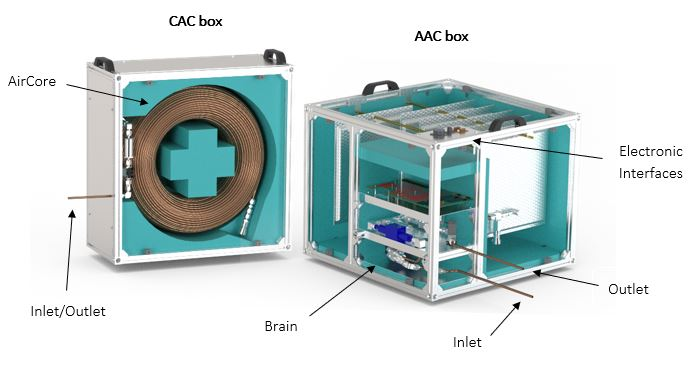
\includegraphics[width=1\linewidth]{4-experiment-design/img/Mechanical/tubular_render_labels.jpg}
    \end{align*}
    \caption{Physical Setup of the Experiment.}
    \label{fig:3D_tubular_render}
\end{figure}

\begin{figure}[H]
    \begin{align*}
        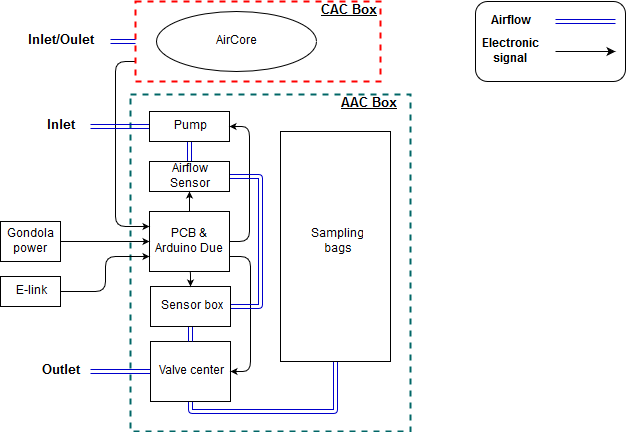
\includegraphics[width=1\linewidth]{4-experiment-design/img/Mechanical/Block-Diagram.png}
    \end{align*}
    \caption{Block Diagram of the Experiment.}
    \label{fig:block-diagram}
\end{figure}

The primary concern regarding the AAC air sampling subsystem \DIFdelbegin \DIFdel{occurs }\DIFdelend \DIFaddbegin \DIFadd{occured }\DIFaddend after the cut-off \DIFdelbegin \DIFdel{when the gondola will tumble and fall }\DIFdelend \DIFaddbegin \DIFadd{while the gondola was tumbling and falling }\DIFaddend at an average speed of 50 m/s for approximately two minutes \cite{BexusManual}. This descent speed \DIFdelbegin \DIFdel{is }\DIFdelend \DIFaddbegin \DIFadd{was }\DIFaddend too large in order to sample air at the desired vertical resolution, capped at 500 m. As such, sampling \DIFdelbegin \DIFdel{can }\DIFdelend \DIFaddbegin \DIFadd{could }\DIFaddend only be done after the gondola \DIFdelbegin \DIFdel{has }\DIFdelend \DIFaddbegin \DIFadd{had }\DIFaddend stabilized at a descent speed  of 8 m/s \cite{BexusManual}. The tumbling phase \DIFdelbegin \DIFdel{will vertically span for approximately 6 km. Considering }\DIFdelend \DIFaddbegin \DIFadd{was vertically spanned for approximately 8 km. With }\DIFaddend a Float Phase altitude of \DIFdelbegin \DIFdel{25 }\DIFdelend \DIFaddbegin \DIFadd{approximately 27.3 }\DIFaddend km, sampling during the Descent Phase \DIFdelbegin \DIFdel{will commence }\DIFdelend \DIFaddbegin \DIFadd{would have commenced }\DIFaddend at approximately 19 km in altitude. However, the primary region of interest in terms of sampling \DIFdelbegin \DIFdel{is }\DIFdelend \DIFaddbegin \DIFadd{was }\DIFaddend in the stratosphere, particularly between 19 km and \DIFdelbegin \DIFdel{25 }\DIFdelend \DIFaddbegin \DIFadd{27.3 }\DIFaddend km in altitude. \DIFdelbegin \DIFdel{Sampling will thus }\DIFdelend \DIFaddbegin \DIFadd{This was why sampling was planned to }\DIFaddend also occur during the Ascent Phase. Out of the six sampling bags present in the payload, two \DIFdelbegin \DIFdel{will }\DIFdelend \DIFaddbegin \DIFadd{were planned to }\DIFaddend be used during the Ascent Phase at 18 km and 21 km and four during the Descent Phase at 17.5 km, 16 km, 14 km and 12 km as seen in Table \ref{tab:minimum-volume}. Details regarding the sampling strategy can be found in Appendix \ref{sec:appH}.

%\begin{table}[H]
\centering
\begin{tabular}{|c|c|c|c|}
\hline
\multicolumn{1}{|l|}{} & \multicolumn{1}{l|}{\textbf{Sampling Altitudes}} & \multicolumn{1}{l|}{\textbf{Ambient Pressure}} & \multicolumn{1}{l|}{\textbf{Ambient Temperature}} \\ \hline
\multirow{2}{*}{\textbf{Ascent Phase}} & 18 km & 75.0 hPa & 216.7 K \\ \cline{2-4} 
 & 21 km & 46.8 hPa & 217.6 K \\ \hline
\multirow{4}{*}{\textbf{Descent Phase}} & 17.5 km & 81.2 hPa & 216.7 K \\ \cline{2-4} 
 & 16 km & 102.9 hPa & 216.7 K \\ \cline{2-4} 
 & 14 km & 141.0 hPa & 216.7 K \\ \cline{2-4} 
 & 12 km & 193.3 hPa & 216.7 K \\ \hline
\end{tabular}
\caption{Sampling Altitudes as well as the Corresponding Ambient Pressures and Temperatures According to the 1976 US Standard Atmosphere.}
\label{tab:sampling-altitudes}
\end{table}
The maximum pressure that the sampling bags \DIFdelbegin \DIFdel{can withstand has }\DIFdelend \DIFaddbegin \DIFadd{could withstand had }\DIFaddend to be taken into account in order to avoid bursting. Decreasing pressure during the Ascent Phase \DIFdelbegin \DIFdel{poses }\DIFdelend \DIFaddbegin \DIFadd{would have posed }\DIFaddend a risk to sampling bags which already \DIFdelbegin \DIFdel{contain }\DIFdelend \DIFaddbegin \DIFadd{contained }\DIFaddend samples as the gas inside \DIFdelbegin \DIFdel{will }\DIFdelend \DIFaddbegin \DIFadd{would }\DIFaddend expand which may cause the bag to burst. In order to avoid this, the sampling bags \DIFdelbegin \DIFdel{will not }\DIFdelend \DIFaddbegin \DIFadd{were not planned to }\DIFaddend be completely filled. Filling the \DIFaddbegin \DIFadd{sampling }\DIFaddend bags up to a maximum pressure of 2 psi/0.14 bar/140 hPa or alternatively filling the sampling bag up to 80\% of its capacity  \DIFdelbegin \DIFdel{is }\DIFdelend \DIFaddbegin \DIFadd{was }\DIFaddend recommended by the manufacturers for the Multi-Layer Foil sampling bags that \DIFdelbegin \DIFdel{are to be }\DIFdelend \DIFaddbegin \DIFadd{were }\DIFaddend used. Therefore, the \DIFdelbegin \DIFdel{maximum expected }\DIFdelend \DIFaddbegin \DIFadd{expected maximum }\DIFaddend pressure inside the bags, that \DIFdelbegin \DIFdel{will be }\DIFdelend \DIFaddbegin \DIFadd{were }\DIFaddend filled during the Ascent Phase, \DIFdelbegin \DIFdel{will }\DIFdelend \DIFaddbegin \DIFadd{would }\DIFaddend be 1.6 psi/0.11 bar/110 hPa. The inverse \DIFdelbegin \DIFdel{is }\DIFdelend \DIFaddbegin \DIFadd{was }\DIFaddend also true for the Descent Phase where compression \DIFdelbegin \DIFdel{will }\DIFdelend \DIFaddbegin \DIFadd{would }\DIFaddend occur. As such, the sampling bags \DIFdelbegin \DIFdel{should }\DIFdelend \DIFaddbegin \DIFadd{had to }\DIFaddend be fully filled during the Descent Phase in order to ensure that enough samples \DIFdelbegin \DIFdel{are }\DIFdelend \DIFaddbegin \DIFadd{were }\DIFaddend collected for analysis. During the Descent Phase, the \DIFaddbegin \DIFadd{expected }\DIFaddend maximum pressure inside the bags \DIFdelbegin \DIFdel{is }\DIFdelend \DIFaddbegin \DIFadd{was }\DIFaddend expected to be 1.98 psi/0.13 bar/130 hPa. Past research \DIFdelbegin \DIFdel{has }\DIFdelend \DIFaddbegin \DIFadd{had }\DIFaddend revealed that the selected sampling bags \DIFdelbegin \DIFdel{can }\DIFdelend \DIFaddbegin \DIFadd{were able to }\DIFaddend withstand pressure difference of 310 hPa at 30 km of altitude, which \DIFdelbegin \DIFdel{is }\DIFdelend \DIFaddbegin \DIFadd{was }\DIFaddend equivalent to 0.31 bar \cite{LISA}. Test 16 and 18, shown in Table \ref{tab:sampling-system-test} respective Table \ref{tab:pump-low-pressure-test},  \DIFdelbegin \DIFdel{will be }\DIFdelend \DIFaddbegin \DIFadd{were }\DIFaddend conducted in order to confirm the maximum allowable pressure for the bags.

The maximum operating pressure for the tubes, according to the manufacturers, \DIFdelbegin \DIFdel{is }\DIFdelend \DIFaddbegin \DIFadd{was }\DIFaddend 2.2 psi/0.15 bar/150 hPa. The valve's leakage rate, given by the manufacturers, \DIFdelbegin \DIFdel{is }\DIFdelend \DIFaddbegin \DIFadd{was }\DIFaddend 0.001 l/min.     


Due to the difference in pressure between sea level and sampling altitudes, the volume of the sample taken \DIFdelbegin \DIFdel{will be }\DIFdelend \DIFaddbegin \DIFadd{would have been }\DIFaddend considerably reduced when it \DIFdelbegin \DIFdel{reaches }\DIFdelend \DIFaddbegin \DIFadd{reached }\DIFaddend sea level. This shrinking \DIFdelbegin \DIFdel{has }\DIFdelend \DIFaddbegin \DIFadd{had }\DIFaddend to be taken into account as the minimum volume that \DIFdelbegin \DIFdel{has }\DIFdelend \DIFaddbegin \DIFadd{had }\DIFaddend to be present in the sampling bag at sea level in order to obtain results with the Picarro analyzer. A minimum amount \DIFdelbegin \DIFdel{is }\DIFdelend \DIFaddbegin \DIFadd{was }\DIFaddend required for the analyzer to detect concentrations of the targeted trace gases. This minimum amount \DIFdelbegin \DIFdel{is }\DIFdelend \DIFaddbegin \DIFadd{was }\DIFaddend 0.18 L at sea level and it \DIFdelbegin \DIFdel{has }\DIFdelend \DIFaddbegin \DIFadd{had }\DIFaddend to be specially considered for the samples taken at higher altitudes. The samples taken at lower altitudes \DIFdelbegin \DIFdel{will be }\DIFdelend \DIFaddbegin \DIFadd{were }\DIFaddend exposed to smaller changes in pressure, therefore their size \DIFdelbegin \DIFdel{will not be }\DIFdelend \DIFaddbegin \DIFadd{was not }\DIFaddend critically reduced. Table \ref{tab:minimum-volume} shows the minimum volume of air that \DIFdelbegin \DIFdel{needs }\DIFdelend \DIFaddbegin \DIFadd{was needed }\DIFaddend to be sampled at different altitudes in order to assure the minimum air sample of 0.18L left at sea level. \\

This \DIFdelbegin \DIFdel{is }\DIFdelend \DIFaddbegin \DIFadd{was }\DIFaddend the worst case scenario, and testing \DIFdelbegin \DIFdel{has }\DIFdelend \DIFaddbegin \DIFadd{had }\DIFaddend shown that the higher the volume of the air sample left at sea level, the better the results. This \DIFdelbegin \DIFdel{is }\DIFdelend \DIFaddbegin \DIFadd{was }\DIFaddend why the aimed volume of the samples, at sea level \DIFdelbegin \DIFdel{will be }\DIFdelend \DIFaddbegin \DIFadd{was }\DIFaddend at least 0.6L. 

%and the corresponding temperature and pressure conditions
 %pressure and temperature (288 K)  
% Depending on the sampling altitude,there is a minimum volume of air that needs to be sampled in order the sample volume left at sea level pressure is at least 0.18 L. A sample volume of 0.18 L corresponds to the minimum amount required for the Picarro analyzer to detect concentrations of the targeted trace gases. 

% Please add the following required packages to your document preamble:
% \usepackage{multirow}
\begin{table}[H]
\centering
\begin{tabular}{|l|l|l|l|l|}
\hline
 & \textbf{\begin{tabular}[c]{@{}l@{}}Minimum \\ Sampling Volume\end{tabular}} & \textbf{\begin{tabular}[c]{@{}l@{}}Sampling \\ Altitudes\end{tabular}} & \textbf{\begin{tabular}[c]{@{}l@{}}Ambient \\ Pressure\end{tabular}} & \textbf{\begin{tabular}[c]{@{}l@{}}Ambient \\ Temperature\end{tabular}} \\ \hline
\multirow{2}{*}{\textbf{Ascent Phase}} & 1.8 L & 18 km & 75.0 hPa & 216.7 K \\ \cline{2-5} 
 & 2.4 L & 21 km & 46.8 hPa & 217.6 K \\ \hline
\multirow{4}{*}{\textbf{Descent Phase}} & 1.7 L & 17.5 km & 81.2 hPa & 216.7 K \\ \cline{2-5} 
 & 1.3 L & 16 km & 102.9 hPa & 216.7 K \\ \cline{2-5} 
 & 1.0 L & 14 km & 141.0 hPa & 216.7 K \\ \cline{2-5} 
 & 0.7 L & 12 km & 193.3 hPa & 216.7 K \\ \hline
\end{tabular}
\caption{Sampling Altitudes as well as the Corresponding Ambient Pressures and Temperatures According to the 1976 US Standard Atmosphere and the Minimum Sampling Volume at Each Altitude to Obtain Enough Air to Perform a Proper Analysis (0.18 L at Sea Level), Appendix \ref{sec:appH}.}
\label{tab:minimum-volume}
\end{table}


The AAC \DIFdelbegin \DIFdel{will need }\DIFdelend \DIFaddbegin \DIFadd{needed }\DIFaddend an air pump for sampling due to low ambient pressure at stratospheric altitudes. The air pump \DIFdelbegin \DIFdel{is }\DIFdelend \DIFaddbegin \DIFadd{was }\DIFaddend also needed in order to assure the intake flow rate and obtain a good resolution. An air pump with an intake rate of at least 3 L/min \DIFdelbegin \DIFdel{will be }\DIFdelend \DIFaddbegin \DIFadd{was }\DIFaddend used to ensure that the vertical resolution of the sampling air \DIFdelbegin \DIFdel{remains }\DIFdelend \DIFaddbegin \DIFadd{remained }\DIFaddend under 500 m during the Ascent Phase's ascent speed of 5 m/s and the  Descent Phase's descent speed of 8 m/s. A flushing valve (see Figure \ref{pneumatic_system}, No.23) \DIFdelbegin \DIFdel{will be }\DIFdelend \DIFaddbegin \DIFadd{was }\DIFaddend used to flush the AAC system before each bag \DIFdelbegin \DIFdel{is }\DIFdelend \DIFaddbegin \DIFadd{would have been }\DIFaddend filled and make sure that each bag \DIFdelbegin \DIFdel{will be }\DIFdelend \DIFaddbegin \DIFadd{would have been }\DIFaddend filled with fresh air from the corresponding altitude. This filling/flushing procedure \DIFdelbegin \DIFdel{occurs }\DIFdelend \DIFaddbegin \DIFadd{was planned to occur }\DIFaddend twice, the first time during the Ascent Phase for the first two sampling bags and the second time during the Descent Phase for the remaining four sampling bags.

Shortly after the launch, the CAC valve \DIFdelbegin \DIFdel{will be }\DIFdelend \DIFaddbegin \DIFadd{was }\DIFaddend opened in order to allow the fill gas that \DIFdelbegin \DIFdel{is }\DIFdelend \DIFaddbegin \DIFadd{was }\DIFaddend inside the tube to flush, while the AAC valves \DIFdelbegin \DIFdel{will be }\DIFdelend \DIFaddbegin \DIFadd{were }\DIFaddend closed until reaching the sampling altitude. Flushing of the CAC tube \DIFdelbegin \DIFdel{happens }\DIFdelend \DIFaddbegin \DIFadd{happened }\DIFaddend passively through the progressive decrease in air pressure during the balloon's Ascent Phase and it \DIFdelbegin \DIFdel{will be }\DIFdelend \DIFaddbegin \DIFadd{was }\DIFaddend emptied by the time it \DIFdelbegin \DIFdel{reaches }\DIFdelend \DIFaddbegin \DIFadd{reached }\DIFaddend the Float Phase. Filling of the CAC tube also \DIFdelbegin \DIFdel{happens }\DIFdelend \DIFaddbegin \DIFadd{happened }\DIFaddend passively through the progressive increase in air pressure during the balloon's Descent Phase. The CAC valve \DIFdelbegin \DIFdel{will }\DIFdelend \DIFaddbegin \DIFadd{was planned to  }\DIFaddend remain open at all time during the Ascent, Float, and Descent phases. \DIFdelbegin \DIFdel{The valve will close }\DIFdelend \DIFaddbegin \DIFadd{Due to some problems, it was briefly closed and opened again for a few times without really compromising the results.  The valve should have been closed }\DIFaddend just before hitting the ground in order to preserve the sample. 

The ambient pressure \DIFdelbegin \DIFdel{will be }\DIFdelend \DIFaddbegin \DIFadd{was }\DIFaddend measured by three pressure sensors located outside the experiment box. Only one of them \DIFdelbegin \DIFdel{is }\DIFdelend \DIFaddbegin \DIFadd{was }\DIFaddend necessary for AAC and CAC, but using three\DIFdelbegin \DIFdel{will provide redundancy }\DIFdelend \DIFaddbegin \DIFadd{, redundancy was provided}\DIFaddend . To measure the pressure inside the bag that \DIFdelbegin \DIFdel{is }\DIFdelend \DIFaddbegin \DIFadd{was }\DIFaddend currently being filled, one analogue static pressure sensor \DIFdelbegin \DIFdel{will be }\DIFdelend \DIFaddbegin \DIFadd{was }\DIFaddend connected to the pneumatic system. To measure the ambient temperature in the CAC, three sensors \DIFdelbegin \DIFdel{will be }\DIFdelend \DIFaddbegin \DIFadd{were }\DIFaddend allocated in the CAC box (in the Styrofoam). Temperature inside the coil \DIFdelbegin \DIFdel{is }\DIFdelend \DIFaddbegin \DIFadd{was }\DIFaddend assumed to quickly adjust to the ambient temperature inside the CAC box, therefore there \DIFdelbegin \DIFdel{will }\DIFdelend \DIFaddbegin \DIFadd{would }\DIFaddend not be differentiation in temperature between the air inside the tube and the air surrounding the tube. For the bags three more temperature sensors \DIFdelbegin \DIFdel{will be }\DIFdelend \DIFaddbegin \DIFadd{were }\DIFaddend placed in the bags' box (in the Styrofoam). To control the temperature for the pump and the valves in pneumatic subsystem, one temperature sensor \DIFdelbegin \DIFdel{will be }\DIFdelend \DIFaddbegin \DIFadd{was }\DIFaddend used for each of them. In total, there \DIFdelbegin \DIFdel{will be }\DIFdelend \DIFaddbegin \DIFadd{were }\DIFaddend three pressure sensors and eight temperature sensors. 

The sampling of the AAC \DIFdelbegin \DIFdel{will be }\DIFdelend \DIFaddbegin \DIFadd{was }\DIFaddend triggered by the pressure reading from the sensors outside the experiment box. When the required pressure \DIFdelbegin \DIFdel{is }\DIFdelend \DIFaddbegin \DIFadd{was }\DIFaddend reached, as seen in Table \ref{tab:minimum-volume} the valve inside the manifold corresponding to the bag that \DIFdelbegin \DIFdel{is }\DIFdelend \DIFaddbegin \DIFadd{was }\DIFaddend to be sampled, \DIFdelbegin \DIFdel{will open }\DIFdelend \DIFaddbegin \DIFadd{should have opened }\DIFaddend and the sampling \DIFdelbegin \DIFdel{will start}\DIFdelend \DIFaddbegin \DIFadd{should have started}\DIFaddend . The closing of the valve \DIFdelbegin \DIFdel{depends }\DIFdelend \DIFaddbegin \DIFadd{depended }\DIFaddend on two conditions and it \DIFdelbegin \DIFdel{will be }\DIFdelend \DIFaddbegin \DIFadd{was }\DIFaddend triggered when either one of the conditions \DIFdelbegin \DIFdel{is }\DIFdelend \DIFaddbegin \DIFadd{was }\DIFaddend true. These conditions \DIFdelbegin \DIFdel{are}\DIFdelend \DIFaddbegin \DIFadd{were}\DIFaddend : maximum sampling time or maximum pressure difference between inside/outside the bags. They \DIFdelbegin \DIFdel{are }\DIFdelend \DIFaddbegin \DIFadd{were }\DIFaddend determined from past research \cite{LISA}. A first estimation of the maximum sampling time \DIFdelbegin \DIFdel{has }\DIFdelend \DIFaddbegin \DIFadd{had }\DIFaddend already been made, from Test 18 shown in Table \ref{tab:pump-low-pressure-test}. Completed tests, such as Test 14 and Test 18, shown in Table \ref{tab:vacuum-test} respective Table \ref{tab:pump-low-pressure-test}, the maximum pressure condition \DIFdelbegin \DIFdel{has }\DIFdelend \DIFaddbegin \DIFadd{had }\DIFaddend been determined and the maximum sampling times \DIFdelbegin \DIFdel{have }\DIFdelend \DIFaddbegin \DIFadd{had }\DIFaddend been confirmed.

The CAC emptying as well as the AAC and CAC sampling sequence is represented in Figures \ref{fig:ascent} and \ref{fig:descent}. It should be kept in mind that the different pressures \DIFdelbegin \DIFdel{are what triggers }\DIFdelend \DIFaddbegin \DIFadd{were what should have triggered }\DIFaddend the opening of the valves. 

\begin{figure}[H]
    \begin{align*}
        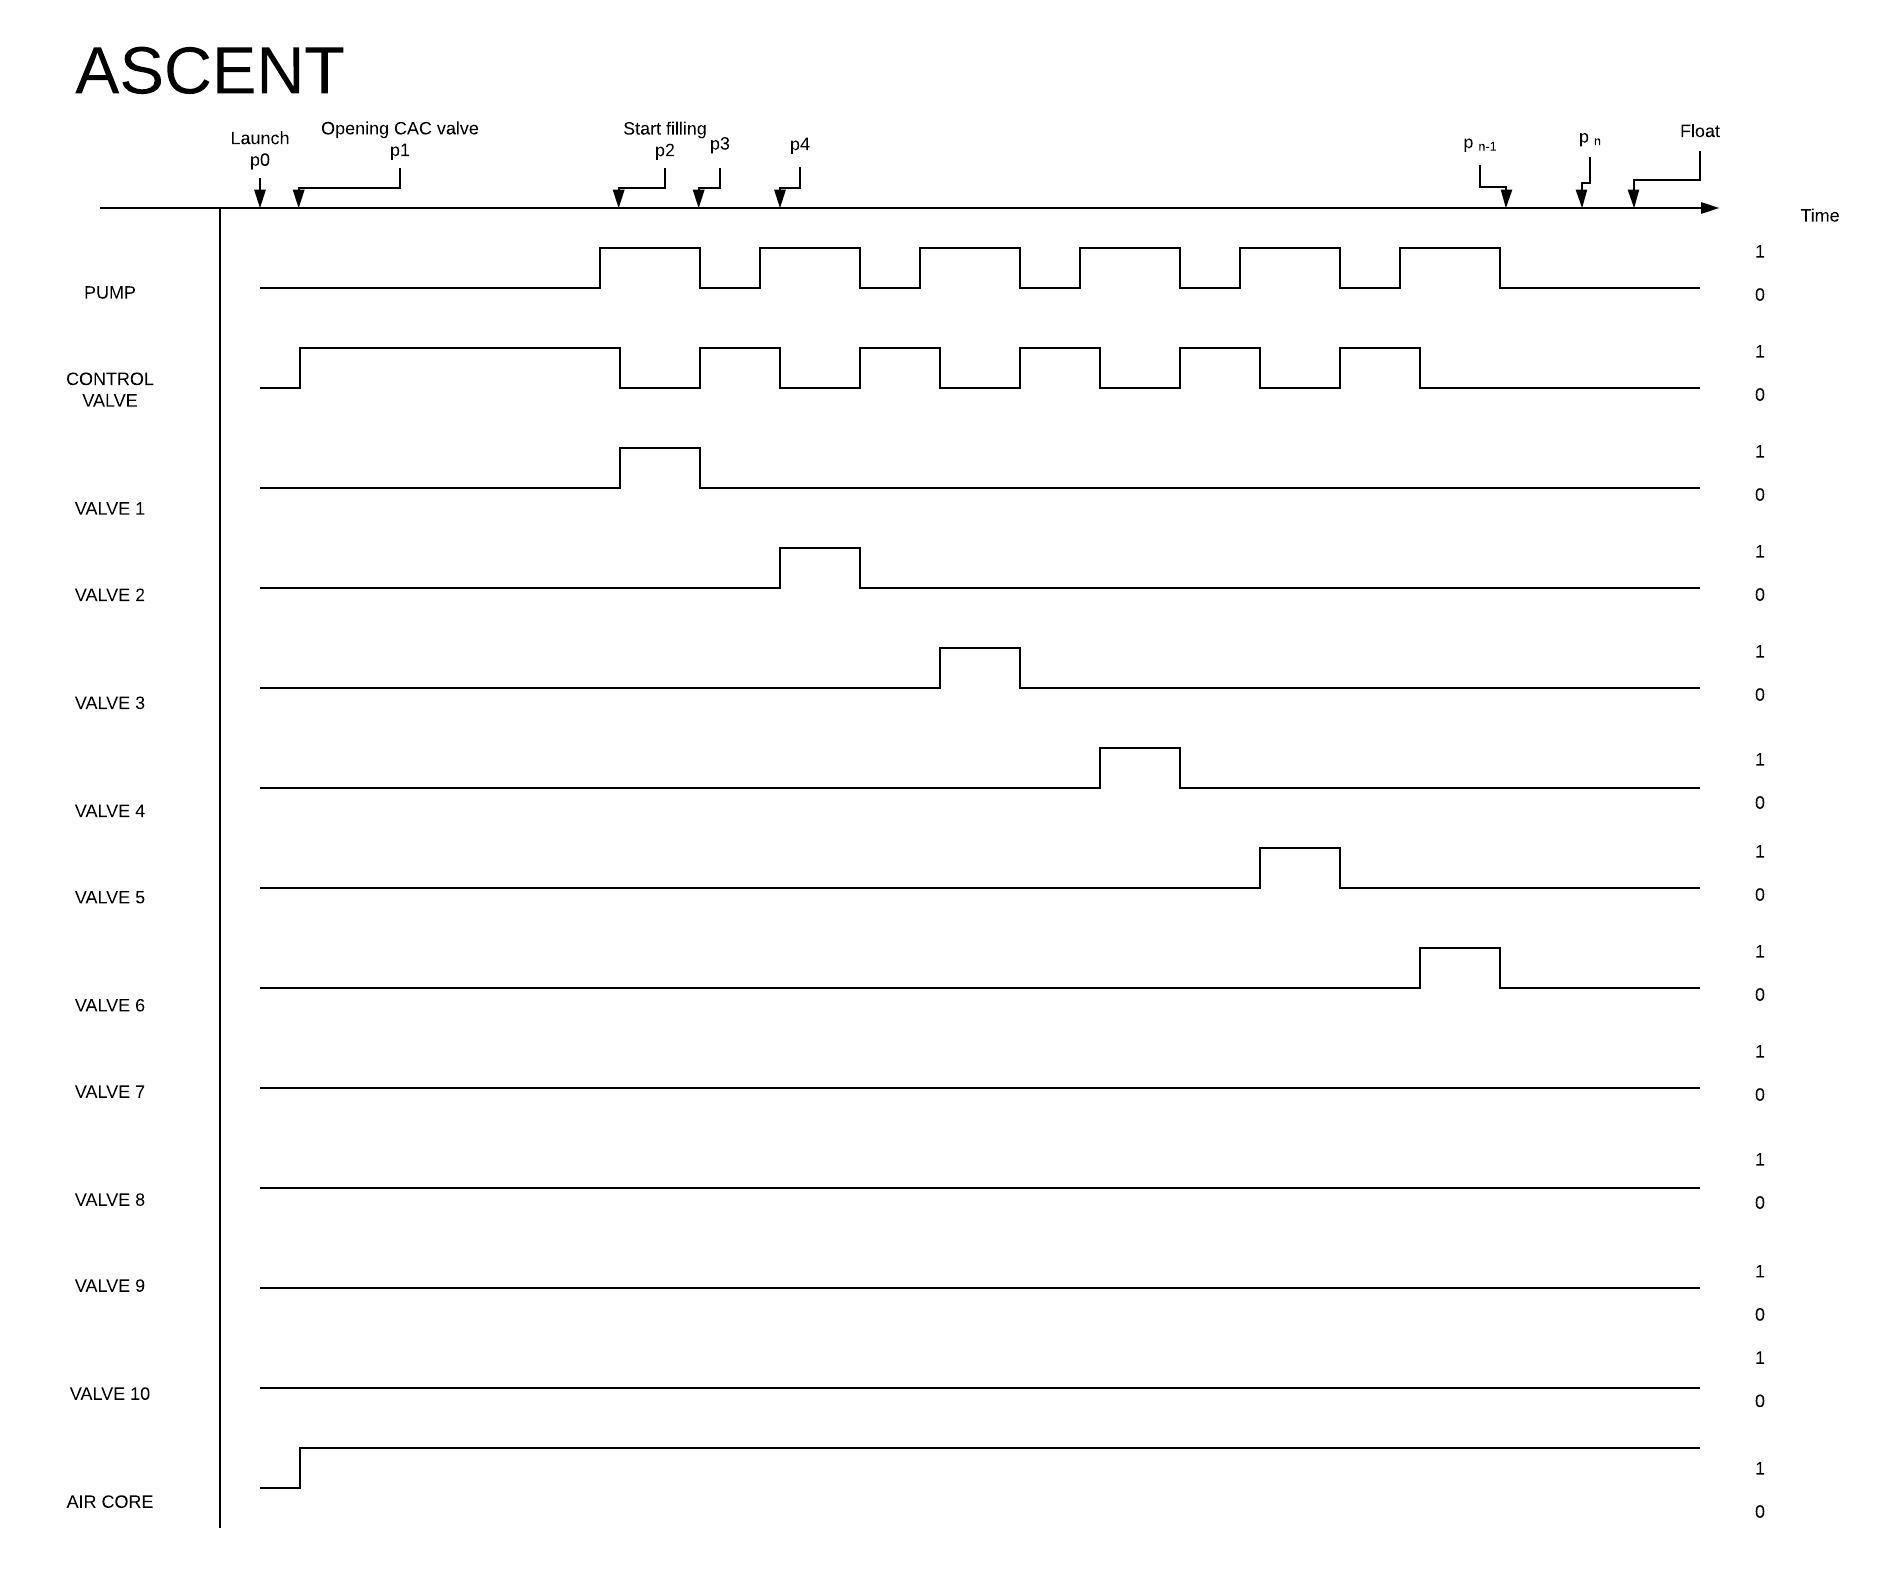
\includegraphics[width=1\linewidth]{4-experiment-design/img/ascent-phase.jpeg}
    \end{align*}
    \caption{The Emptying and Sampling Sequence-Ascent Phase.}
    \label{fig:ascent}
\end{figure}

\begin{figure}[H]
    \begin{align*}
        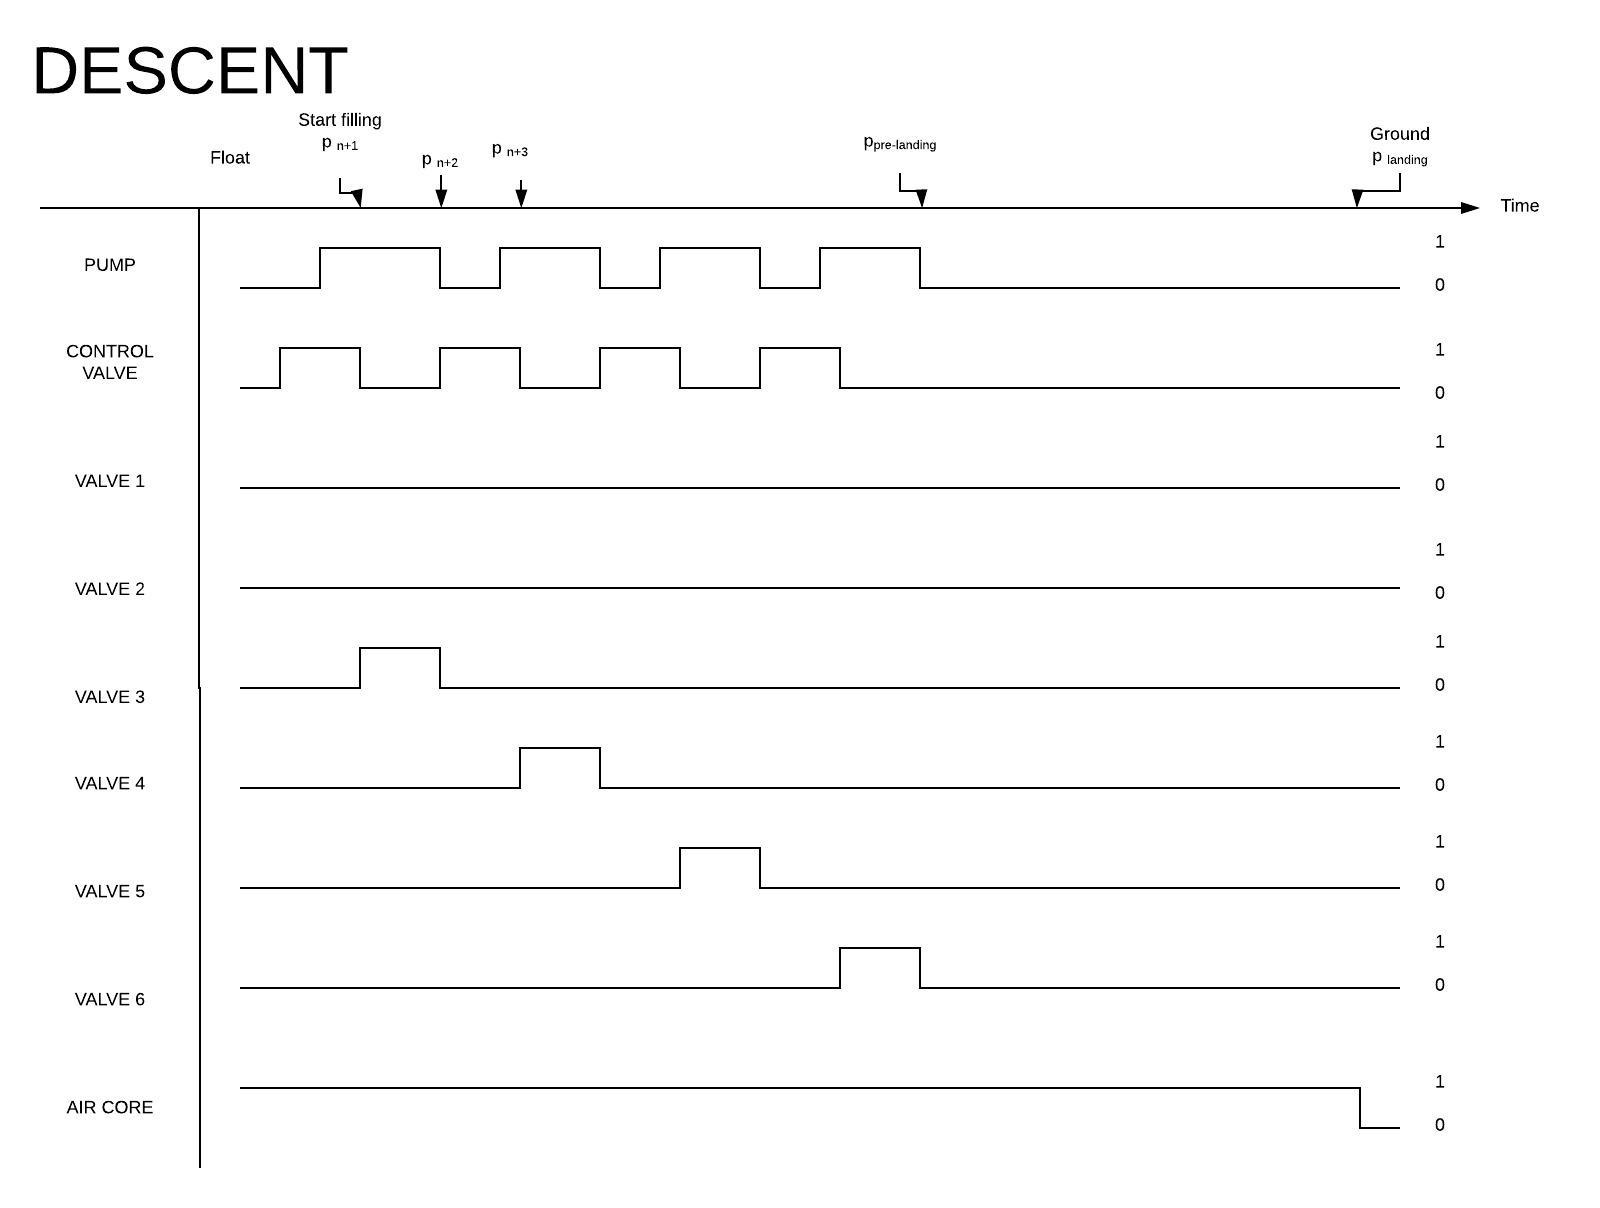
\includegraphics[width=1\linewidth]{4-experiment-design/img/descent-phase.jpeg}
    \end{align*}
    \caption{The Emptying and Sampling Sequence-Descent Phase.\label{fig:descent}}
\end{figure}

In the diagrams, 0 denotes closed/off and 1 denotes opened/on. The horizontal axis denotes the different pressure levels throughout the flight, with p$_0$ being the sea level pressure and p$_8$ being the pressure during Float Phase.

The ambient pressure dependent timeline of the experiment \DIFdelbegin \DIFdel{is }\DIFdelend \DIFaddbegin \DIFadd{was planned to be }\DIFaddend as follow:

\textbf{Ascent Phase:}\\
$p_0$ – $p_1$
\begin{itemize}
    \item CAC valve shall be closed.
    \item AAC valves shall be closed.
    \end{itemize}
$p_1$ – $p_2$
\begin{itemize}
    \item CAC valve shall be opened.
    \item CAC tube shall start flushing.
    \end{itemize}

$p_2$ – $p_3$
\begin{itemize}
    \item AAC flushing valve shall be opened, allowing for the system to flush.
    \item CAC valve \DIFdelbegin \DIFdel{remains }\DIFdelend \DIFaddbegin \DIFadd{should remain }\DIFaddend open.
    \end{itemize}
$p_3$ – $p_4$
\begin{itemize}
    \item AAC flushing valve shall be closed.
    \item Valve 1 shall be opened, allowing for air to enter the first bag.
    \item CAC valve \DIFdelbegin \DIFdel{remains }\DIFdelend \DIFaddbegin \DIFadd{should remain }\DIFaddend open.
    \end{itemize}
$p_4$ – $p_5$
\begin{itemize}
    \item Valve 1 shall be closed.
    \item AAC flushing valve shall be closed.
    \item CAC valve \DIFdelbegin \DIFdel{remains }\DIFdelend \DIFaddbegin \DIFadd{should  remain }\DIFaddend open.
    \end{itemize}
$p_5$ - $p_6$    
 \begin{itemize}
    \item AAC flushing valve shall be opened, allowing the system to flush. 
    \item CAC valve \DIFdelbegin \DIFdel{remains }\DIFdelend \DIFaddbegin \DIFadd{should remain }\DIFaddend open.
    \end{itemize}
$p_6$ - $p_7$
\begin{itemize}
    \item AAC flushing valve shall be closed.
    \item Valve 2 shall be opened, allowing for air to enter the second bag.
    \item CAC valve \DIFdelbegin \DIFdel{remains }\DIFdelend \DIFaddbegin \DIFadd{should remain }\DIFaddend open.
    \end{itemize}
$p_7$ - $p_8$
\begin{itemize}
    \item Valve 2 shall be closed.
    \item AAC flushing valve shall be closed.
    \item CAC shall finish flushing.
    \end{itemize}    




\textbf{\\Float Phase:}\\
No action \DIFdelbegin \DIFdel{is }\DIFdelend \DIFaddbegin \DIFadd{was }\DIFaddend taken other than continued telemetry.

\textbf{Descent Phase:}

$p_9$ – $p_{10}$
\begin{itemize}
    \item CAC shall start sampling. 
    \item AAC valves shall be closed.
\end{itemize}

$p_{10}$ – $p_{11}$
\begin{itemize}
    \item AAC flushing valve shall be opened allowing the system to flush.
    \item CAC valve \DIFdelbegin \DIFdel{remains }\DIFdelend \DIFaddbegin \DIFadd{should remain }\DIFaddend open. 
\end{itemize}

  
$p_{11}$ – $p_{12}$
\begin{itemize}
    \item AAC flushing valve shall be closed.
    \item Valve 3 shall be opened, allowing for air to enter the third bag.
    \item CAC valve \DIFdelbegin \DIFdel{remains }\DIFdelend \DIFaddbegin \DIFadd{should remain }\DIFaddend open. 
\end{itemize}

$p_{12}$ – $p_{13}$
\begin{itemize}
    \item Valve 3 shall be closed.
    \item AAC flushing valve shall be closed.
    \item CAC valve \DIFdelbegin \DIFdel{remains }\DIFdelend \DIFaddbegin \DIFadd{should remain }\DIFaddend open.
\end{itemize}

$p_{13}$ – $p_{14}$
\begin{itemize}
    \item AAC flushing valve shall be opened allowing the system to flush.
    \item CAC valve \DIFdelbegin \DIFdel{remains }\DIFdelend \DIFaddbegin \DIFadd{should remain }\DIFaddend open.
\end{itemize}

$p_{14}$ – $p_{15}$
\begin{itemize}
    \item AAC flushing valve shall be closed.
    \item Valve 4 shall be opened, allowing for air to enter the fourth bag.
    \item CAC valve \DIFdelbegin \DIFdel{remains }\DIFdelend \DIFaddbegin \DIFadd{should remain }\DIFaddend open.
\end{itemize}

$p_{15}$ – $p_{16}$
\begin{itemize}
    \item Valve 4 shall be closed.
    \item AAC flushing valve shall be closed.
    \item CAC valve \DIFdelbegin \DIFdel{remains }\DIFdelend \DIFaddbegin \DIFadd{should remain }\DIFaddend open.
\end{itemize}

$p_{16}$ – $p_{17}$
\begin{itemize}
    \item AAC flushing valve shall be opened, allowing the system to flush. 
    \item CAC \DIFdelbegin \DIFdel{remains }\DIFdelend \DIFaddbegin \DIFadd{should remain }\DIFaddend open.
  \end{itemize}

$p_{17}$ – $p_{18}$
\begin{itemize}
    \item AAC flushing valve shall be closed.
    \item Valve 5 shall be opened, allowing for air to enter the fifth bag. 
    \item CAC valve \DIFdelbegin \DIFdel{remains }\DIFdelend \DIFaddbegin \DIFadd{should remain }\DIFaddend open.
\end{itemize}

$p_{18}$ – $p_{19}$
\begin{itemize}
    \item Valve 5 shall be closed.
    \item AAC flushing valve shall be closed.
    \item CAC valve \DIFdelbegin \DIFdel{remains }\DIFdelend \DIFaddbegin \DIFadd{should remain }\DIFaddend open.
\end{itemize}

$p_{19}$ – $p_{20}$
\begin{itemize}
     \item AAC flushing valve shall be opened, allowing the system to flush. 
    \item CAC \DIFdelbegin \DIFdel{remains }\DIFdelend \DIFaddbegin \DIFadd{valve should remain }\DIFaddend open.
   \end{itemize}

$p_{20}$ – $p_{21}$
\begin{itemize}
    \item AAC flushing valve shall be closed.
    \item Valve 6 shall be opened, allowing for air to enter the sixth bag.
    \DIFaddbegin \item \DIFadd{CAC valve should remain open.
}\DIFaddend \end{itemize}

$p_{pre-landing}$ 
\begin{itemize}
    \item Valve 6 shall be closed.
    \item AAC flushing valve shall be closed.
    \item CAC valve shall be opened.
\end{itemize}

$p_{0-landing}$
\begin{itemize}
    \item CAC valve shall be closed.
\end{itemize}


Note: The AAC system's air pump is only on during sampling into the air sampling bags and flushing of the system.


\raggedbottom
\pagebreak
\subsection{Experiment Interfaces}

\subsubsection{Mechanical Interfaces}
\label{sec:4.2.1}

\bigskip
\begin{table}[H]
\noindent\makebox[\columnwidth]{%
\scalebox{0.8}{
\begin{tabular}{|c|c|c|c|c|c|}
\hline
\textbf{Component} & \textbf{Interface} & \textbf{Amount} & \textbf{Dimensions} &  \begin{tabular}[c]{@{}c@{}}\textbf{Total}\\ \textbf{weight}\end{tabular}  \\ \hline
Bracket standard 20/20 slot 6/6 & AAC-Gondola & $8$ & $20 \times 20 \times 20\ mm$ & $40\ g$ \\ \hline
Tolerance holes bracket & CAC-Gondola & $2$ & $ 20 \times 30 \times 52 \ mm$ & $50\ g$ \\ \hline
4-hole plate & AAC-CAC & $6$ & $1 \times 60 \times 45\ mm$ & $100\ g$ \\ \hline
Rubber bumpers M6 & AAC-Gondola, CAC-Gondola & $10$ & $19 \times 19 \times 15\ mm$ & $300\ g$ \\ \hline
T-nut slot 6 M4 & AAC-CAC, AAC-Gondola, CAC-Gondola & $44$ & $4 \times 5.9 \times 11.5\ mm$ & $132\ g$ \\ \hline
T-nut slot 8 M6 & AAC-Gondola, CAC-Gondola & $10$ & $6 \times 11 \times 16\ mm$ &  $60\ g$ \\ \hline

Steel bolt M4 & AAC-CAC, AAC-Gondola & $44$ & $8\ mm $ length & $34\ g$ \\ \hline
Steel washer M4 & AAC-CAC, AAC-Gondola & $24$ &\begin{tabular}[c]{@{}c@{}}$ID=4.3\ mm$\\ $OD=9\ mm$\end{tabular} &  $4.8\ g$\\ \hline
% Polyamide bolt M4 & Styrofoam-CAC-AAC & $8$ & $20\ mm $ length & $3\ g$ & $24\ g$ \\ \hline
% Polyamide washer M4 & Styrofoam-CAC-AAC & $8$ &\begin{tabular}[c]{@{}c@{}}$ID=4.3\ mm$\\ $OD=25\ mm$\end{tabular} & $4\ g$ & $32\ g$\\ \hline
Styrofoam bars  & AAC-Gondola, CAC-Gondola & $4$ & see Appendix \ref{sec:mech_drawings} & $450\ g$ \\ \hline
Handles  & CAC \& AAC & $4$ & $ 18.6 \times 25.2 \times 112.5 \ mm$ & $80\ g$ \\ \hline
\end{tabular}}}
\caption{Summary of Gondola-AAC-CAC Interfaces Components.}
\label{table:attaching-components}
\end{table}


\underline{Gondola - TUBULAR joining}

\smallskip
The experiment box \DIFdelbegin \DIFdel{will be }\DIFdelend \DIFaddbegin \DIFadd{was }\DIFaddend fixed to the gondola rails by means of $10$ brackets interfacing the experiment outside structure with the hammer nuts in the rails. Two different types of brackets \DIFdelbegin \DIFdel{are }\DIFdelend \DIFaddbegin \DIFadd{were }\DIFaddend used to be flexible with respect to the gondola rails distances, which can be modified by use after previous BEXUS campaigns. Eight small $20/20$ brackets (Figure \ref{fig:bracket_small}) \DIFdelbegin \DIFdel{are }\DIFdelend \DIFaddbegin \DIFadd{were }\DIFaddend used to fix the AAC box to specific rails placement, and two other big brackets (Figure \ref{fig:bracket_big}) \DIFdelbegin \DIFdel{are }\DIFdelend \DIFaddbegin \DIFadd{were }\DIFaddend used to fix the CAC box to the nearest rail. This method is secure as well as fast enough to provide an accessible and easy recovery for later analysis.

\begin{figure}[H]
    \noindent\makebox[\textwidth]{%
    \begin{subfigure}{.3\textwidth}
        \centering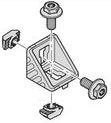
\includegraphics[width=0.55\textwidth]{4-experiment-design/img/Mechanical/bracket.jpg}
        \caption{Rexroth 20/20.}
        \label{fig:bracket_small}
    \end{subfigure}
    \hspace{1cm}
    \begin{subfigure}{.3\textwidth}
        \centering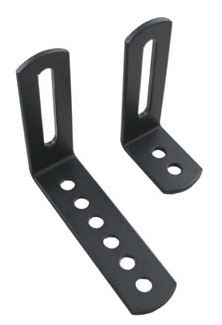
\includegraphics[width=0.55\textwidth,angle=90] {4-experiment-design/img/Mechanical/long_hole_bracket.jpg}
        \caption{Tolerance Holes.}
        \label{fig:bracket_big}
    \end{subfigure}}
    \caption{Bracket Components.}
    \label{fig:bracket}
\end{figure}

\bigskip
\underline{CAC - AAC joining}

\smallskip
A simple but reliable fixing interface between the two boxes of the experiment has been designed to ensure the fast recovery of the CAC box. The latter \DIFdelbegin \DIFdel{requires }\DIFdelend \DIFaddbegin \DIFadd{required }\DIFaddend only unscrewing 12 bolts as well as unplugging a D-Sub connector marked in RED, see Figure \ref{fig:electrical_interfaces}. Once the CAC box \DIFdelbegin \DIFdel{is }\DIFdelend \DIFaddbegin \DIFadd{was }\DIFaddend detached, the AAC Box \DIFdelbegin \DIFdel{will still remain perfectly }\DIFdelend \DIFaddbegin \DIFadd{still remained }\DIFaddend fixed in the gondola. Table \ref{table:attaching-components} includes all the components required to fix the experiment to the gondola.

\bigskip
\underline{Handles}

\smallskip
Four top handles, as shown in Figure \ref{fig:handles} \DIFdelbegin \DIFdel{will be }\DIFdelend \DIFaddbegin \DIFadd{were }\DIFaddend mounted to facilitate the experiment box manipulation when moving it in and out of the gondola.

\begin{figure}[H]
    \centering
    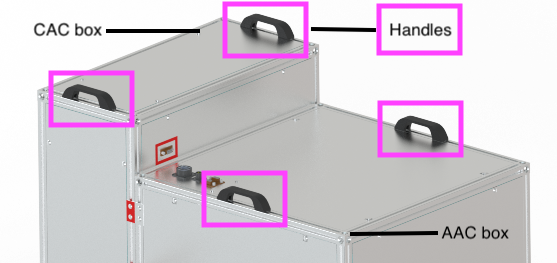
\includegraphics[width=0.8\textwidth]{4-experiment-design/img/Mechanical/Figure_8.png}
    \caption{Handling Interfaces.}
    \label{fig:handles}
\end{figure}

\bigskip
\underline{Inlet/Outlet Pipes}
\label{subsec:pipes}

\smallskip
In order to collect reliable air samples, the experiment \DIFdelbegin \DIFdel{requires }\DIFdelend \DIFaddbegin \DIFadd{was required }\DIFaddend to be mounted with at least one side exposed to the outside. This \DIFdelbegin \DIFdel{will reduce }\DIFdelend \DIFaddbegin \DIFadd{reduced }\DIFaddend the pipe length used to collect clean air. As it can be seen in Figure \ref{fig:3D_tubular_render}, three pipes \DIFdelbegin \DIFdel{will extend }\DIFdelend \DIFaddbegin \DIFadd{were extended }\DIFaddend from the experiment box face: one for the CAC sampling and two, input and output, for the AAC sampling. 

These pipes \DIFdelbegin \DIFdel{are }\DIFdelend \DIFaddbegin \DIFadd{were }\DIFaddend welded/drawn $304$ grade stainless steel tubes from RESTEK company, which \DIFdelbegin \DIFdel{are }\DIFdelend \DIFaddbegin \DIFadd{were }\DIFaddend specially recommended for chromatography applications and gas delivery systems with low pressures and inert environments. These tubes \DIFdelbegin \DIFdel{are }\DIFdelend \DIFaddbegin \DIFadd{were }\DIFaddend sulfinert, which is a required treatment for metal components when analyzing for parts-per-billion levels of organo-sulfur compounds.

The tubes, which \DIFdelbegin \DIFdel{are the same that will be }\DIFdelend \DIFaddbegin \DIFadd{were the same ones }\DIFaddend used in the pneumatic system of the \emph{Brain} (see Section \ref{sec:4.4.5}), \DIFdelbegin \DIFdel{have }\DIFdelend \DIFaddbegin \DIFadd{had }\DIFaddend an outer diameter $OD = 6.35\ mm$ ($1/4$ inches) and an inner diameter $ID = 4.57\ mm$ ($0.18$ inches).

\bigskip
\underline{Pump vibration}
\label{subsec:vibration}

To mitigate the vibrations produced by the pump, an extra piece of styrofoam has been added between the pump's anchor plate and the surface of the level 1 of the brain, where this key component is fixed. 


\subsubsection{Thermal Interfaces}
\label{sec:4.2.2}

Both main structural components and external walls of the two boxes of the experiment \DIFdelbegin \DIFdel{are }\DIFdelend \DIFaddbegin \DIFadd{were }\DIFaddend made by aluminum and steel components. For this reason, since these \DIFdelbegin \DIFdel{are }\DIFdelend \DIFaddbegin \DIFadd{were }\DIFaddend conductive materials, a direct attachment to the gondola creates many heat paths with the internal space and subsystems of the experiment. Considering that the temperature gradient between the gondola and the operative requirements of the electronic components can be quite high, this conductive connections drastically decrease the efficiency of the thermal insulation. Therefore, a system based on rubber bumpers and styrofoam bars (see Figure \ref{fig:thermal_interface}) has been designed to remove heat bridges and minimize temperature leaks from the inside of the experiment to the outside.

Figure \ref{fig:rubber_bumper} shows a CAD model of the bumper component and how it looks like when attached to the gondola with the brackets explained in the previous section.

\begin{figure}[H]
    \noindent\makebox[\textwidth]{%
    \begin{subfigure}{.3\textwidth}
        \centering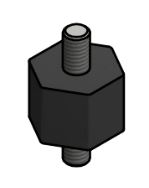
\includegraphics[width=0.55\textwidth]{4-experiment-design/img/Mechanical/rubber_bumper.jpg}
    \end{subfigure}
    \hspace{1cm}
    \begin{subfigure}{.3\textwidth}
        \centering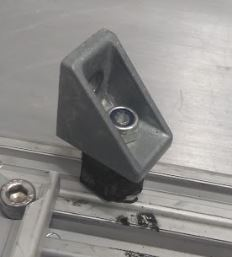
\includegraphics[width=0.55\textwidth] {4-experiment-design/img/Mechanical/real_bumper.jpg}
    \end{subfigure}}
    \caption{Rubber Bumper.}
    \label{fig:rubber_bumper}
\end{figure}

The styrofoam bars \DIFdelbegin \DIFdel{will be }\DIFdelend \DIFaddbegin \DIFadd{were }\DIFaddend attached directly to the rails of the experiment structure by M4 plastic screws and big washers.

\begin{figure}[H]
    \centering
    \DIFdelbeginFL %DIFDELCMD < 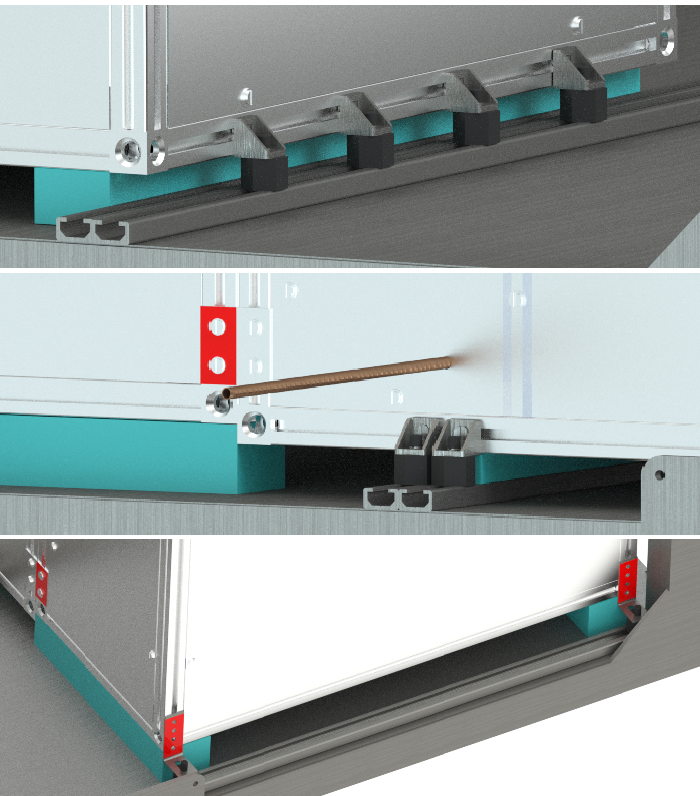
\includegraphics[width=0.6\textwidth]{4-experiment-design/img/Mechanical/gondola_fixation.png}
%DIFDELCMD <     %%%
\DIFdelendFL \DIFaddbeginFL 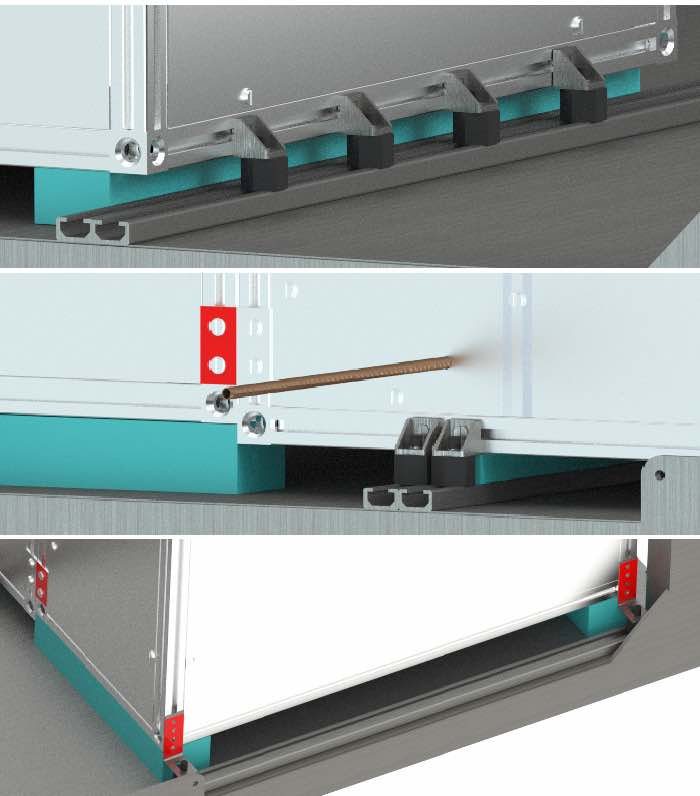
\includegraphics[width=0.6\textwidth]{4-experiment-design/img/Mechanical/gondola_fixation.jpg}
    \DIFaddendFL \caption{Thermal Interfaces TUBULAR-Gondola.}
    \label{fig:thermal_interface}
\end{figure}

\subsubsection{CAC Interfaces}
An uncoupled quick connector, shown in Figure \ref{fig:Quick-connector-body}, \DIFdelbegin \DIFdel{will be }\DIFdelend \DIFaddbegin \DIFadd{was }\DIFaddend attached at each end of the coiled tube to seal the opening. It \DIFdelbegin \DIFdel{will remain }\DIFdelend \DIFaddbegin \DIFadd{remained }\DIFaddend tightly sealed until the quick connectors \DIFdelbegin \DIFdel{are }\DIFdelend \DIFaddbegin \DIFadd{were }\DIFaddend manually coupled. 

\begin{figure}[H]
    \centering
    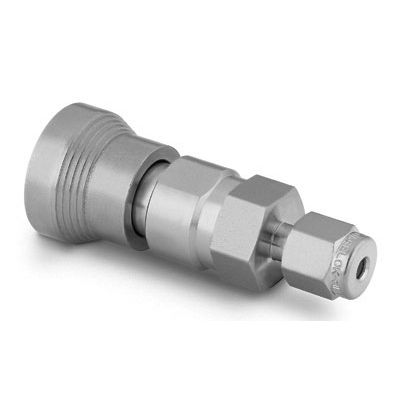
\includegraphics[width=0.2\textwidth]{4-experiment-design/img/Mechanical/CAC-QC-Outlet.jpg}
    \caption{Swagelok Quick Connector Body.}
    \label{fig:Quick-connector-body}
\end{figure}

The interfaces between the other parts in the CAC set up \DIFdelbegin \DIFdel{will be }\DIFdelend \DIFaddbegin \DIFadd{were }\DIFaddend joined with specific tube fittings, listed in Table \ref{tab:CAC-interfaces}. All the chosen interfaces \DIFdelbegin \DIFdel{are }\DIFdelend \DIFaddbegin \DIFadd{were }\DIFaddend from Swagelok. Using products from the same manufacture minimizes the risk for leakage or mismatched interfaces in the system. 

\begin{table}[H]
\centering
\scalebox{0.8}{
\begin{tabular}{|c|c|c|c|}
\hline
\textbf{Component}                                                          & \textbf{Interface}             & \textbf{Amount} & \textbf{Fitting Size}                                                    \\ \hline
\begin{tabular}[c]{@{}c@{}}Quick connector body\\ SS-QC4-B-200\end{tabular} & Outlet of coiled tube          & 1               & 1/8 in.                                                                  \\ \hline
\begin{tabular}[c]{@{}c@{}}Quick connector body\\ SS-QC4-B-400\end{tabular} & Inlet of coiled tube           & 1               & 1/4 in.                                                                  \\ \hline
\begin{tabular}[c]{@{}c@{}}Quick connector stem\\ SS-QC4-D-400\end{tabular} & Inlet of coiled tube -  Filter & 1               & 1/4 in.                                                                  \\ \hline
\begin{tabular}[c]{@{}c@{}}Male connector\\ SS-400-1-2\end{tabular}             & Tube fitting - Solenoid valve   & 2               & \begin{tabular}[c]{@{}c@{}}Tube OD 1/8 in. to \\ Tube OD 1/4 in.\end{tabular}    \\ \hline
\begin{tabular}[c]{@{}c@{}}Straight Tube Union\\ SS-200-6\end{tabular}             & Quick connector 1/8 in. - Tube 1/8 in.     & 1               & 1/8 in.
\\ \hline
\begin{tabular}[c]{@{}c@{}}Tube Reducer\\ SS-400-6-2 \end{tabular}             & Tube 1/8 in. - Tube 1/4 in.     & 1               & \begin{tabular}[c]{@{}c@{}}Tube OD 1/8 in. to \\ Tube OD 1/4 in.\end{tabular}
\\ \hline
\begin{tabular}[c]{@{}c@{}}Straight Tube Union\\ SS-400-6\end{tabular}             & Tube 1/4 in. - 90 degree connector    & 1               & 1/4 in.
\\ \hline
\begin{tabular}[c]{@{}c@{}}Union 90-degree connector\\ SS-400-9\end{tabular}             &
\begin{tabular}[c]{@{}c@{}} Between certain tube fittings\\ Outlet tube \end{tabular} & 3               & 1/4 in.
\\ \hline
\begin{tabular}[c]{@{}c@{}}Tube fitting\\ SS-401-PC\end{tabular}             & \begin{tabular}[c]{@{}c@{}} Between certain tube fittings\\ Magnesium dryer filter \end{tabular} & 5               & 1/4 in.
\\ \hline
\end{tabular}}
\caption{Interfaces within CAC Setup.}
\label{tab:CAC-interfaces}
\end{table}

\subsubsection{AAC Interfaces}
In the AAC system, the interfaces between various components \DIFdelbegin \DIFdel{are }\DIFdelend \DIFaddbegin \DIFadd{were }\DIFaddend a mixture of eleven different types of tube fittings from Swagelok. The selected types \DIFdelbegin \DIFdel{are }\DIFdelend \DIFaddbegin \DIFadd{were }\DIFaddend straight and elbow union, T-union, female and male elbows, male and female connectors, tube fittings, and quick coupling with a certain  specifications. Some of them are shown in Figure \ref{fig:AAC-interfaces-fittings}. Information regarding the fitting's placement in the AAC and fitting sizes are summarized in Table \ref{tab:AAC-interfaces}. 

\begin{figure}[H]
    \centering
    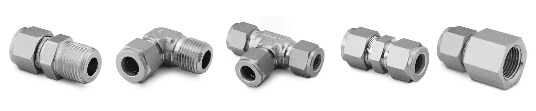
\includegraphics[width=0.8\textwidth]{4-experiment-design/img/Mechanical/AAC-interfaces.jpg}
    \caption{From Left to Right: Male Connector, Male Elbow, T-union, Straight Union and Female Connector.}
    \label{fig:AAC-interfaces-fittings}
\end{figure}

\begin{table}[H]
\centering
\DIFdelbeginFL %DIFDELCMD < \scalebox{0.8}{
%DIFDELCMD < \begin{tabular}{|c|c|c|c|}
%DIFDELCMD < \hline
%DIFDELCMD < \textbf{Component}                                                    & \textbf{Interface}                                                                                                                                                                         & \textbf{Amount} & \textbf{Fitting Size}                                                                     \\ \hline
%DIFDELCMD < \begin{tabular}[c]{@{}c@{}}Male connector\\ SS-400-1-2\end{tabular}   & \begin{tabular}[c]{@{}c@{}} Tube to Manifold - Flushing valve\\ Flushing valve - Outlet tube\\ Manifold valve - Tube to bag\end{tabular} & 8              & \begin{tabular}[c]{@{}c@{}}Male 1/8 in. to \\ Tube OD 1/4 in.\end{tabular}  \\ \hline
%DIFDELCMD < \begin{tabular}[c]{@{}c@{}}Male connector\\ SS-400-1-4\end{tabular}   & \begin{tabular}[c]{@{}c@{}} Manifold - Tube to Flushing valve\end{tabular} & 1              & \begin{tabular}[c]{@{}c@{}}Male 1/4 in. to \\ Tube OD 1/4 in.\end{tabular}  \\ \hline
%DIFDELCMD < \begin{tabular}[c]{@{}c@{}}Male elbow\\ SS-400-2-4\end{tabular}       & \begin{tabular}[c]{@{}c@{}}Static pressure sensor - Manifold \end{tabular}                                                                                                                                                            & 1               & \begin{tabular}[c]{@{}c@{}}Male 1/4 in. to \\ Tube OD 1/4 in. \end{tabular}  \\ \hline
%DIFDELCMD < \begin{tabular}[c]{@{}c@{}}Female elbow\\ SS-400-8-4\end{tabular}       & \begin{tabular}[c]{@{}c@{}}Pump tube - Airflow sensor \\ Airflow sensor -  Static pressure sensor    \end{tabular}                                                                                                                                                        & 2               & \begin{tabular}[c]{@{}c@{}}Female 1/4 in. to \\ Tube OD 1/4 in. in.\end{tabular}  \\ \hline
%DIFDELCMD < \begin{tabular}[c]{@{}c@{}}Female connector\\ SS-4-TA-7-4RG\end{tabular}       & \begin{tabular}[c]{@{}c@{}}Static pressure sensor - T-Union   \end{tabular}                                                                                                                                                        & 1               & \begin{tabular}[c]{@{}c@{}}Female 1/4 in. and \\ Tube OD 1/4 in. in.\end{tabular}  \\ \hline
%DIFDELCMD < \begin{tabular}[c]{@{}c@{}}Straight union\\ SS-400-6\end{tabular}     & \begin{tabular}[c]{@{}c@{}}Filter - Tube filter\\ Tube filter - Pump\end{tabular}                                                                                       & 3               & \begin{tabular}[c]{@{}c@{}}Tube OD 1/4 in.\end{tabular}                     \\ \hline
%DIFDELCMD < \begin{tabular}[c]{@{}c@{}}Elbow union\\ SS-400-9\end{tabular}       & \begin{tabular}[c]{@{}c@{}}Pump tube - Filter tube    \end{tabular}                                                                                                                                                        & 1               & \begin{tabular}[c]{@{}c@{}}Tube OD 1/4 in. in.\end{tabular}  \\ \hline
%DIFDELCMD < \begin{tabular}[c]{@{}c@{}}T-Union\\ SS-400-3\end{tabular}            & \begin{tabular}[c]{@{}c@{}}Static pressure sensor    \end{tabular}                                                                                                                                                                 & 3               & Tube OD 1/4 in.                                                                              \\ \hline
%DIFDELCMD < \begin{tabular}[c]{@{}c@{}}T-Union\\ SS-400-3-4TTM\end{tabular}            & Tube valve - Bag valve   - Quick Connector                                                                                                                                                                & 5               &\begin{tabular}[c]{@{}c@{}} Male 1/4 in. and \\  2 x Tube OD 1/4 in.   \end{tabular}                                                                           \\ \hline
%DIFDELCMD < \begin{tabular}[c]{@{}c@{}}T-Union\\ SS-400-3-4TMT\end{tabular}            & Tube valve - Bag valve - Quick Connector                                                                                                                                                              & 1                & \begin{tabular}[c]{@{}c@{}}Male 1/4 in. \\ 2 x Tube OD 1/4 in.   \end{tabular}                                                                           \\ \hline
%DIFDELCMD < \begin{tabular}[c]{@{}c@{}}T-Union\\ SS-6M0-3\end{tabular}            & Pump Inlet and Outlet                                                                                                                                                             & 2                & \begin{tabular}[c]{@{}c@{}} Tube OD 6mm   \end{tabular}                                                                           \\ \hline
%DIFDELCMD < \begin{tabular}[c]{@{}c@{}}Tube Fitting\\ SS-401-PC\end{tabular}            & Filter - Pump                                                                                                                                                              & 1                & \begin{tabular}[c]{@{}c@{}} Tube OD 1/4in.   \end{tabular}                                                                           \\ \hline
%DIFDELCMD < \begin{tabular}[c]{@{}c@{}}Tube Fitting Reducer\\ SS-400-R-6M\end{tabular}            &\begin{tabular}[c]{@{}c@{}} Filter - Pump  \\ Pump - Airflow sensor    \end{tabular}                                                                                                                                                         & 2                & \begin{tabular}[c]{@{}c@{}} Tube OD 1/4in. to \\ Tube OD 6mm   \end{tabular}                                                                           \\ \hline
%DIFDELCMD < \begin{tabular}[c]{@{}c@{}}Tube Inserts\\ SS-6M5-4M\end{tabular}            & Pump Inlet and Outlet                                                                                                                                                           & 2                & \begin{tabular}[c]{@{}c@{}} OD 6mm - ID 4mm   \end{tabular}                                                                           \\ \hline
%DIFDELCMD < \begin{tabular}[c]{@{}c@{}}Tube Fitting Female \\ SS-4-TA-7-4RG\end{tabular}            &\begin{tabular}[c]{@{}c@{}} Static pressure sensor    \end{tabular}                                                                                                                                                         & 1                & \begin{tabular}[c]{@{}c@{}} Tube OD 1/4in. to \\ female 1/4"    \end{tabular}                                                                           \\ \hline
%DIFDELCMD < \begin{tabular}[c]{@{}c@{}}Quick Coupling \\ SS-QC4-B-4PF\end{tabular}            &\begin{tabular}[c]{@{}c@{}} T-Union of bags    \end{tabular}                                                                                                                                                         & 6                & \begin{tabular}[c]{@{}c@{}} SS female 1/4"    \end{tabular}                                                                           \\ \hline
%DIFDELCMD < \end{tabular}}
%DIFDELCMD < %%%
\DIFdelendFL \DIFaddbeginFL \scalebox{0.8}{
\begin{tabular}{|c|c|c|c|}
\hline
\textbf{Component}                                                    & \textbf{Interface}                                                                                                                                                                         & \textbf{Amount} & \textbf{Fitting Size}                                                                     \\ \hline
\begin{tabular}[c]{@{}c@{}}Male connector\\ SS-400-1-2\end{tabular}   & \begin{tabular}[c]{@{}c@{}} Tube to Manifold - Flushing valve\\ Flushing valve - Outlet tube\\ Manifold valve - Tube to bag\end{tabular} & 8              & \begin{tabular}[c]{@{}c@{}}Male 1/8 in. to \\ Tube OD 1/4 in.\end{tabular}  \\ \hline
\begin{tabular}[c]{@{}c@{}}Male connector\\ SS-400-1-4\end{tabular}   & \begin{tabular}[c]{@{}c@{}} Manifold - Tube to Flushing valve\end{tabular} & 1              & \begin{tabular}[c]{@{}c@{}}Male 1/4 in. to \\ Tube OD 1/4 in.\end{tabular}  \\ \hline
\begin{tabular}[c]{@{}c@{}}Male elbow\\ SS-400-2-4\end{tabular}       & \begin{tabular}[c]{@{}c@{}}Static pressure sensor - Manifold \end{tabular}                                                                                                                                                            & 1               & \begin{tabular}[c]{@{}c@{}}Male 1/4 in. to \\ Tube OD 1/4 in. \end{tabular}  \\ \hline
\begin{tabular}[c]{@{}c@{}}Female elbow\\ SS-400-8-4\end{tabular}       & \begin{tabular}[c]{@{}c@{}}Pump tube - Airflow sensor \\ Airflow sensor -  Static pressure sensor    \end{tabular}                                                                                                                                                        & 2               & \begin{tabular}[c]{@{}c@{}}Female 1/4 in. to \\ Tube OD 1/4 in. in.\end{tabular}  \\ \hline
\begin{tabular}[c]{@{}c@{}}Female connector\\ SS-4-TA-7-4RG\end{tabular}       & \begin{tabular}[c]{@{}c@{}}Static pressure sensor - T-Union   \end{tabular}                                                                                                                                                        & 1               & \begin{tabular}[c]{@{}c@{}}Female 1/4 in. and \\ Tube OD 1/4 in. in.\end{tabular}  \\ \hline
\begin{tabular}[c]{@{}c@{}}Straight union\\ SS-400-6\end{tabular}     & \begin{tabular}[c]{@{}c@{}}Filter - Tube filter\\ Tube filter - Pump\end{tabular}                                                                                       & 3               & \begin{tabular}[c]{@{}c@{}}Tube OD 1/4 in.\end{tabular}                     \\ \hline
\begin{tabular}[c]{@{}c@{}}Elbow union\\ SS-400-9\end{tabular}       & \begin{tabular}[c]{@{}c@{}}Pump tube - Filter tube    \end{tabular}                                                                                                                                                        & 1               & \begin{tabular}[c]{@{}c@{}}Tube OD 1/4 in. in.\end{tabular}  \\ \hline
\begin{tabular}[c]{@{}c@{}}T-Union\\ SS-400-3\end{tabular}            & \begin{tabular}[c]{@{}c@{}}Static pressure sensor    \end{tabular}                                                                                                                                                                 & 3               & Tube OD 1/4 in.                                                                              \\ \hline
\begin{tabular}[c]{@{}c@{}}T-Union\\ SS-400-3-4TTM\end{tabular}            & Tube valve - Bag valve   - Quick Connector                                                                                                                                                                & 5               &\begin{tabular}[c]{@{}c@{}} Male 1/4 in. and \\  2 x Tube OD 1/4 in.   \end{tabular}                                                                           \\ \hline
\begin{tabular}[c]{@{}c@{}}T-Union\\ SS-400-3-4TMT\end{tabular}            & Tube valve - Bag valve - Quick Connector                                                                                                                                                              & 1                & \begin{tabular}[c]{@{}c@{}}Male 1/4 in. \\ 2 x Tube OD 1/4 in.   \end{tabular}                                                                           \\ \hline
\begin{tabular}[c]{@{}c@{}}T-Union\\ SS-6M0-3\end{tabular}            & Pump Inlet and Outlet                                                                                                                                                             & 2                & \begin{tabular}[c]{@{}c@{}} Tube OD 6mm   \end{tabular}                                                                           \\ \hline
\begin{tabular}[c]{@{}c@{}}Tube Fitting\\ SS-401-PC\end{tabular}            & Filter - Pump                                                                                                                                                              & 1                & \begin{tabular}[c]{@{}c@{}} Tube OD 1/4in.   \end{tabular}                                                                           \\ \hline
\begin{tabular}[c]{@{}c@{}}Tube Fitting Reducer\\ SS-400-R-6M\end{tabular}            &\begin{tabular}[c]{@{}c@{}} Filter - Pump  \\ Pump - Airflow sensor    \end{tabular}                                                                                                                                                         & 2                & \begin{tabular}[c]{@{}c@{}} Tube OD 1/4in. to \\ Tube OD 6mm   \end{tabular}                                                                           \\ \hline
\begin{tabular}[c]{@{}c@{}}Tube Inserts\\ SS-6M5-4M\end{tabular}            & Pump Inlet and Outlet                                                                                                                                                           & 2                & \begin{tabular}[c]{@{}c@{}} OD 6mm - ID 4mm   \end{tabular}                                                                           \\ \hline
\begin{tabular}[c]{@{}c@{}}Tube Fitting Female \\ SS-4-TA-7-4RG\end{tabular}            &\begin{tabular}[c]{@{}c@{}} Static pressure sensor    \end{tabular}                                                                                                                                                         & 1                & \begin{tabular}[c]{@{}c@{}} Tube OD 1/4in. to \\ female 1/4"    \end{tabular}                                                                           \\ \hline
\begin{tabular}[c]{@{}c@{}}Quick Coupling \\ SS-QC4-B-4PF\end{tabular}            &\begin{tabular}[c]{@{}c@{}} T-Union of bags    \end{tabular}                                                                                                                                                         & 6                & \begin{tabular}[c]{@{}c@{}} SS female 1/4"    \end{tabular}                                                                           \\ \hline
\begin{tabular}[c]{@{}c@{}}Tube adapter \\ SS-300-R-4\end{tabular} &\begin{tabular}[c]{@{}c@{}} T-Union - Bag valve    \end{tabular}                                                                                                                                                         & 6                & \begin{tabular}[c]{@{}c@{}} Tube OD 1/4in. to \\ Tube OD 3/16"    \end{tabular}                                                                           \\ \hline
\end{tabular}}
\DIFaddendFL \caption{Interface Descriptions Inside AAC System.}
\label{tab:AAC-interfaces}
\end{table}


\subsubsection{Electrical Interfaces}
\label{sec:4.2.3}

The experiment \DIFdelbegin \DIFdel{will connect }\DIFdelend \DIFaddbegin \DIFadd{was connected }\DIFaddend to the gondola electrically via a 4 pin, male, box mount receptacle MIL - C-26482P series 1 connector with an 8-4 insert arrangement (MS3112E8-4P) \cite{BexusManual}. It \DIFdelbegin \DIFdel{will connect }\DIFdelend \DIFaddbegin \DIFadd{was connected }\DIFaddend to one 28.8 V/1 mA battery pack which \DIFdelbegin \DIFdel{consists }\DIFdelend \DIFaddbegin \DIFadd{consisted }\DIFaddend of eight SAFT LSH20 batteries in series where each \DIFdelbegin \DIFdel{has }\DIFdelend \DIFaddbegin \DIFadd{had }\DIFaddend a 5 A fuse\cite{BexusManual}. The expected maximum current is 1.1 A.

\begin{figure}[H]
    \centering
    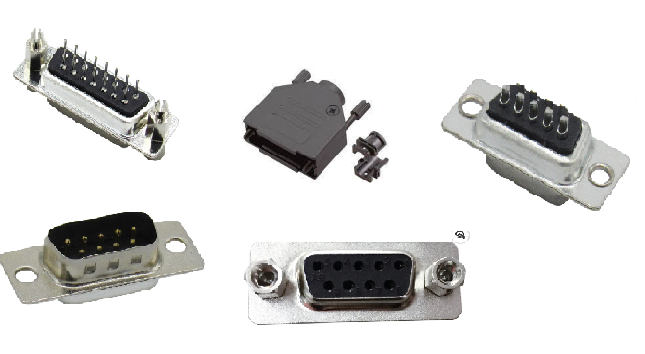
\includegraphics[width=0.4\textwidth]{4-experiment-design/img/connectors.png}
    \caption{Connectors.}
    \label{fig:connectors}
\end{figure}

The E-Link connection shall be made between the experiment and the E-Link system using a RJ45 connection which \DIFdelbegin \DIFdel{will be }\DIFdelend \DIFaddbegin \DIFadd{was }\DIFaddend supplied by SSC and an Ethernet protocol. The Amphenol RJF21B connector \DIFdelbegin \DIFdel{will be }\DIFdelend \DIFaddbegin \DIFadd{was }\DIFaddend mounted on either the front or the side of the experiment\cite{BexusManual}.  

The CAC and AAC \DIFdelbegin \DIFdel{will be }\DIFdelend \DIFaddbegin \DIFadd{were }\DIFaddend connected together with a D-SUB 9-pin connector where power, ground and signals for the sensors in the CAC \DIFdelbegin \DIFdel{will be }\DIFdelend \DIFaddbegin \DIFadd{were }\DIFaddend connected. A female connector \DIFdelbegin \DIFdel{will be }\DIFdelend \DIFaddbegin \DIFadd{was }\DIFaddend located on the AAC wall and a male connector on the CAC wall.

Another female D-SUB 9-pin connector \DIFdelbegin \DIFdel{will be }\DIFdelend \DIFaddbegin \DIFadd{was }\DIFaddend located on the wall of the AAC in which the connections for the three ambient pressure sensors \DIFdelbegin \DIFdel{will be }\DIFdelend \DIFaddbegin \DIFadd{were }\DIFaddend located. Connectors with different pin configuration are shown in Figure \ref{fig:connectors}.

The expected data rate \DIFdelbegin \DIFdel{is }\DIFdelend \DIFaddbegin \DIFadd{was }\DIFaddend 1.58 kbits/s for downlink and 1.08 kbits/s for uplink.

\begin{figure}[H]
    \centering
    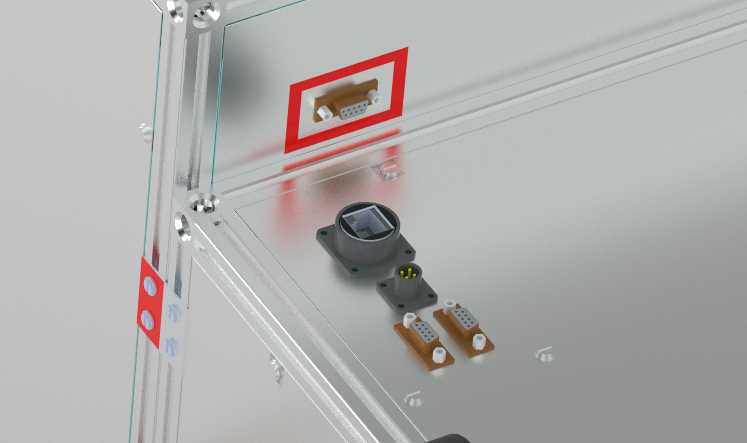
\includegraphics[width=0.8\textwidth]{4-experiment-design/img/Mechanical/Figure_Detail_Interfaces.png}
    \caption{Electrical Interfaces.}
    \label{fig:electrical_interfaces}
\end{figure}



%\begin{figure}[H]
%    \begin{align*}
%        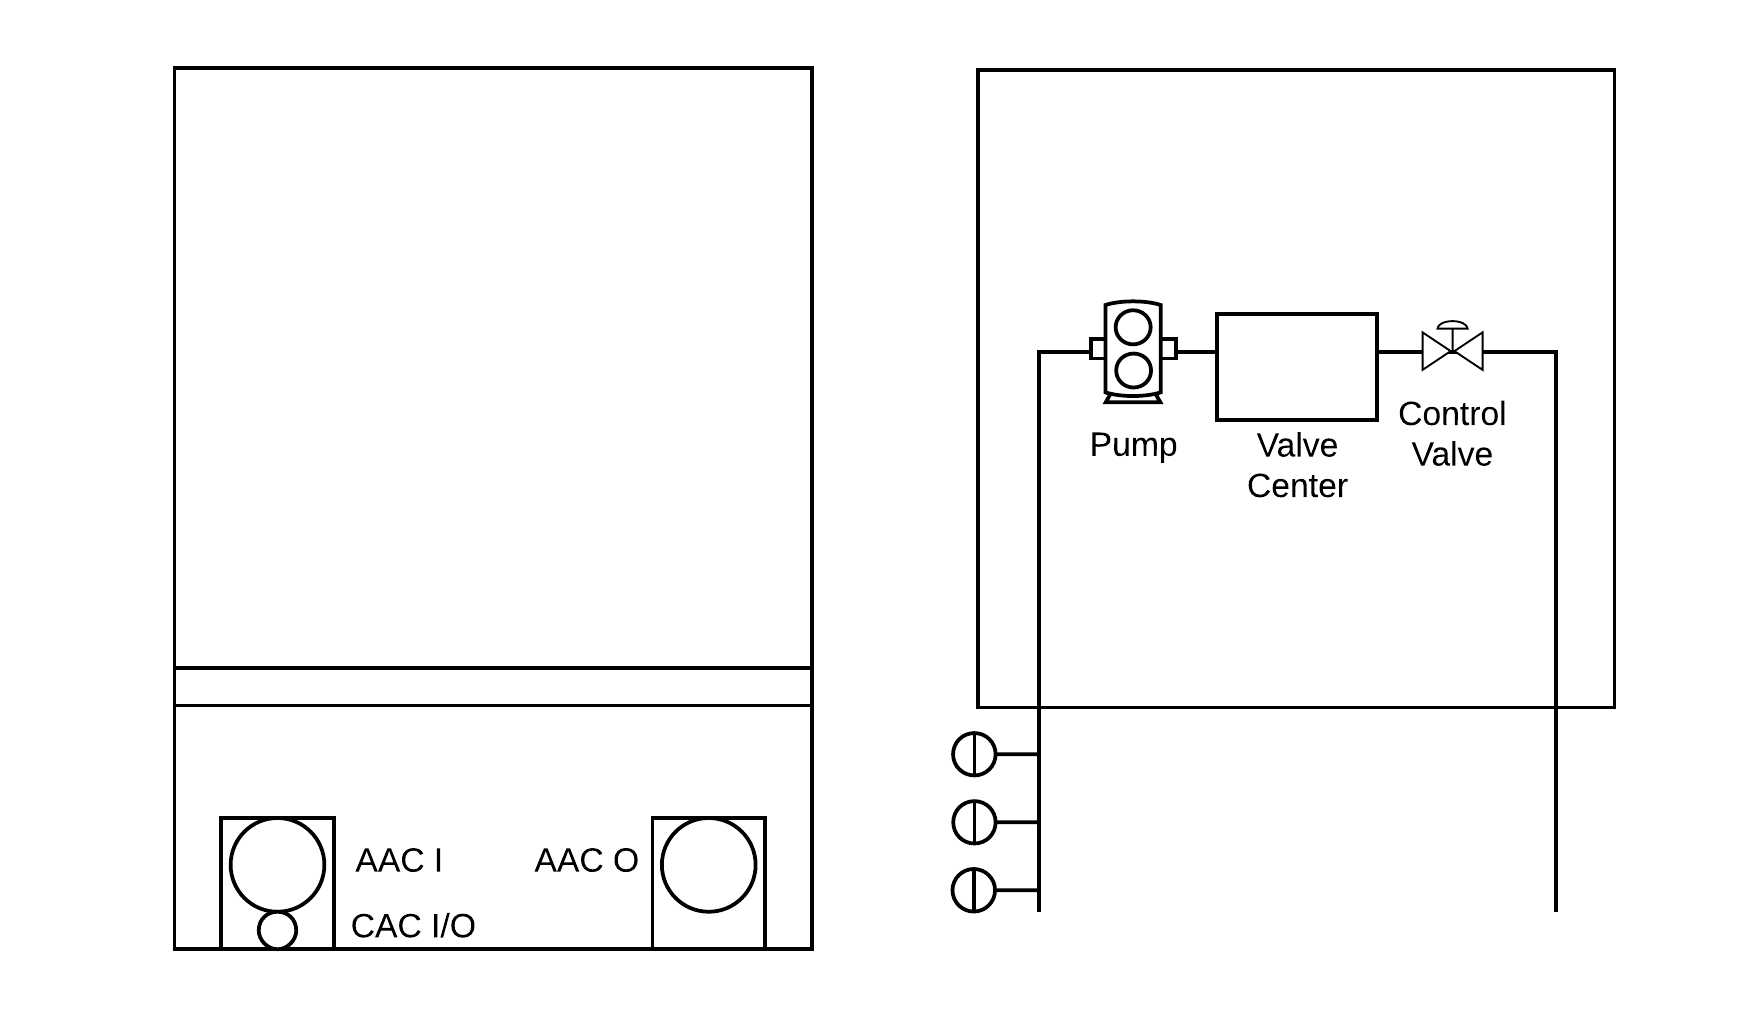
\includegraphics[width=0.7\textwidth]{4-experiment-design/img/Diagram_pipe.png}
%    \end{align*}
%    \caption{Diagram of the experiment box face exposed to the outside.}\label{fig:pipes_interface_1}
%\end{figure}

\iffalse
\subsubsection{Radio Frequencies (Optional)}
\begin{centering}
Not required.
\end{centering}
\bigskip

\subsubsection{Thermal (Optional)}
\begin{centering}
Not required.
\end{centering}
\bigskip
\fi


\raggedbottom
\begin{landscape}
\subsection{Experiment Components} \label{components}
\label{sec:experiment-components}

Component tables were generated from the project budget spreadsheet in Appendix \ref{sec:appO} using the scripts included in Appendix \ref{sec:appK}. 

\subsubsection{Electrical Components}

Table \ref{tab:components-table-electrical} shows all required electrical components with their total mass and price.\\

\begin{longtable} {|m{0.05\textwidth}|m{0.25\textwidth}|m{0.17\textwidth}|m{0.2\textwidth}|m{0.05\textwidth}|m{0.07\textwidth}|m{0.07\textwidth}|m{0.25\textwidth}|m{0.11\textwidth}|} \hline \textbf{ID} & \textbf{Component Name} & \textbf{Manufacturer} & \textbf{Manufacturer Code} & \textbf{Qty} & \textbf{Total Mass [g]} & \textbf{Total Cost [EUR]} & \textbf{Note} & \textbf{Status} \\ \hline E1 & Arduino Due with headers & Arduino & A000062 & 1 & 36 & 35 & Fast and has many analog, and digital pins & Received \\ \hline E2 & Ethernet Shield & SEEED Studio & SKU 103030021 & 1 & 36 & 28 & Can be mounted on top of the board & Received \\ \hline E3 & Miniature diagphram air pump & KNF & NMP 850.1.2 KNDC-B & 1 & 430 & 350 & & Received \\ \hline E4 & Pressure sensor & SENSOR SOLUTIONS & MS560702BA03-50 & 4 & 20 & 9.2 & High resolution, large measuring range & Received \\ \hline E5 & Sampling Valve (inlet and outlet 1/8" female) & SMC & VDW22UANXB & 1 & 100 & 45 & & Received \\ \hline E6 & Airflow sensor & Honeywell & AWM5102VN & 1 & 60 & 130 & 0-10 SLPM & Received \\ \hline E7 & Heater & Minco & HK5160R157L12 & 4 & 16 & 380 & Easy to mount, compact size & Received \\ \hline E9 & Temperature sensor & Maxim Integrated & DS1631+-ND & 8 & 16 & 24 & I2C digital output interface, temperature range down to -55 $\degree{C}$ & Received \\ \hline E10 & DC/DC converter 24 V & Traco Power & S24SP24003PDFA & 2 & 92 & 98 & Provides required output voltage and power, 93\% efficiency & Received \\ \hline E12 & MicroSD & Kingston Technology & SDCIT/16GB & 1 & 0.5 & 20 & Small, good temperature range, sufficient storage & Received \\ \hline E13 & Logic CAT5E Network & Valueline & VLCT85000Y30 & 1 & 90 & 7 & For testing and ground station & Received \\ \hline E14 & Resistors & n/a & n/a & 25 & 25 & 0 & & Received \\ \hline E15 & Capacitors (0.1 uF, 5uF, 10 uF, 100uF) & n/a & n/a & 7 & 7 & 0 & & Received \\ \hline E16 & Mosfet for current control & IR & IRLB8748PBF & 11 & 22 & 7.7 & Cheap, good temperature range & Received \\ \hline E17 & Diodes for DCDC converters & Diotec Semiconductor & 1N5059 & 4 & 1.6 & 0.4 & Cheap, good temperature range & Received \\ \hline E18 & LED 3.3 V & Wurth Elektronik & 151034GS03000 & 16 & 6.4 & 8.3 & For monitoring, testing & Received \\ \hline E19 & 15-pin D-SUB Female connector with pins & RND Connect & RND 205-00779 & 2 & 22 & 1.5 & For connecting distributed components & Received \\ \hline E20 & 9-pin D-SUB Female connector with pins & RND Connect & RND 205-00777 & 3 & 26 & 2 & For connecting distributed components & Received \\ \hline E21 & 9 pin D-SUB Female connector with soldering cups & RND Connect & RND 205-00704 & 3 & 27 & 1.7 & For connecting distributed components & Received \\ \hline E22 & 9 pin D-SUB Male connector with soldering cups & RND Connect & RND 205-00700 & 6 & 54 & 2.9 & For connecting distributed components & Received \\ \hline E23 & 15-pin D-SUB Male connector with soldering cups & RND Connect & RND 205-00701 & 2 & 22 & 1.2 & For connecting distributed components & Received \\ \hline E24 & 9-pin D-SUB backing & Enchitech & MHDTZK-9-BK-K & 6 & 240 & 17 & For connecting distributed components & Received \\ \hline E25 & 15-pin D-SUB backing & Enchitech & MHDTZK-15-BK-K & 2 & 130 & 6.1 & For connecting distributed components & Received \\ \hline E26 & Wall mounting bolts & RND Connect & RND 205-00786 & 3 & 7.5 & 3.1 & For connecting distributed components & Received \\ \hline E28 & 3.3 V Zener diode & RND Components & RND 1N746A & 15 & 7.5 & 1.1 & Regulate indication LED voltage & Received \\ \hline E29 & Male connector on PCB & Binder & Serie 768 & 1 & 5 & 8.5 & & Received \\ \hline E30 & Female connector from wall & Binder & Serie 768 & 1 & 11 & 12 & & Received \\ \hline E31 & Grounding contact & Vogt & DIN 46234 & 4 & 2.3 & 8.6 & 1 pack of 100 pcs & Received \\ \hline E32 & Logic CAT5 E-link for inside box 0.5m & Valueline & VLCP85121E05 & 1 & 20 & 1.3 & To connect from wall to Arduino shield & Received \\ \hline E33 & Signal wire & Alpha Wire & 5854/7 YL005 & 1 & 120 & 34 & Roll of 30 m. Half will be used approximately & Received \\ \hline E34 & Flushing valve (inlet and outlet 1/8" female) & SMC & VDW22UANXB & 1 & 100 & 45 & & Received \\ \hline E35 & Valves manifold (outlet 1/8" female) & SMC & VDW23-5G-1-H-Q & 6 & 600 & 240 & & Received \\ \hline E36 & Power wire - Back & Alpha Wire & 5856 BK005 & 1 & 73 & 46 & Roll of 30 m. A fifth will be used approximately & Received \\ \hline E37 & Electrical Tape for marking wires - White & Hellerman Tyton & HTAPE-FLEX15WH-15X10 & 1 & 14 & 0.82 & Roll of 10 m. A forth will be used approximately & Received \\ \hline E38 & Electrical Tape for marking wires - Black & Hellerman Tyton & HTAPE-FLEX15BK-15X10 & 1 & 13 & 0.82 & Roll of 10 m. A forth will be used approximately & Received \\ \hline E39 & Electrical Tape for marking wires - Green & Hellerman Tyton & HTAPE-FLEX15GN-15X10 & 1 & 14 & 0.82 & Roll of 10 m. A forth will be used approximately & Received \\ \hline E40 & Electrical Tape for marking wires - Violet & Hellerman Tyton & HTAPE-FLEX15VT-15X10 & 1 & 14 & 0.82 & Roll of 10 m. A forth will be used approximately & Received \\ \hline E41 & Electrical Tape for marking wires - Gray & Hellerman Tyton & HTAPE-FLEX15GY-15X10 & 1 & 14 & 0.82 & Roll of 10 m. A forth will be used approximately & Received \\ \hline E42 & Electrical Tape for marking wires - Brown & Hellerman Tyton & HTAPE-FLEX15BN-15X10 & 1 & 14 & 0.82 & Roll of 10 m. A forth will be used approximately & Received \\ \hline E43 & Electrical Tape for marking wires - Blue & Hellerman Tyton & HTAPE-FLEX15BU-15X10 & 1 & 14 & 1.9 & Roll of 10 m. A forth will be used approximately & Received \\ \hline E48 & Power wire - Red & Alpha Wire & 5856 RD005 & 1 & 73 & 46 & Roll of 30 m. A fifth will be used approximately & Received \\ \hline E50 & 6-pin male double row header & RND Connect & RND 205-00634 & 2 & 2 & 0.44 & & Received \\ \hline E51 & 8-pin male single row header & RND Connect & RND 205-00629 & 5 & 5 & 1.4 & & Received \\ \hline E52 & 10-pin male single row header & Prostar & SD-2X5-T1-7/3MM & 1 & 1 & 0.26 & & Received \\ \hline E53 & 36-pin male double row header & Würth Elektronik & 61303621121 & 1 & 2 & 1.7 & & Received \\ \hline E54 & DC/DC converter 12 V & Delta & R-7812-0.5 & 2 & 40 & 68 & 12V,1.67A, 20W DCDC & Received \\ \hline E55 & Potentiometer 50 kOhm & Bourns & 3296Y-1-503LF & 10 & 10 & 18 & & Received \\ \hline E56 & Static Pressure Sensor & Gems Sensors and Controls & 3500S0001A05E000 & 1 & 53 & 120 & & Received \\ \hline E57 & Connector for the Static Pressure Sensor & Schneider Electric & XZCPV1141L2 & 1 & 14 & 14 & -25 to 80 celcius, female 4 pin M12 connector with 2 meter wire & Received \\ \hline E58 & PCB board & Eurocircuits & n/a & 1 & 100 & 180 & Will be custom-made & Received \\ \hline E59 & Pressure sensor PCB & Eurocircuits & n/a & 3 & 75 & 42 & Will be custom-made & Received \\ \hline E60 & Arduino Due without headers & Arduino & 2 & 1 & 36 & 34 & & Received \\ \hline \caption{Electrical Components Table} \label{tab:components-table-electrical} \end{longtable} \raggedbottom

\end{landscape}

\begin{landscape}

\subsubsection{Mechanical Components}

Table \ref{tab:components-table-mechanical} shows all required mechanical components with their total mass and price.\\


\begin{longtable} {|m{0.05\textwidth}|m{0.25\textwidth}|m{0.17\textwidth}|m{0.2\textwidth}|m{0.05\textwidth}|m{0.07\textwidth}|m{0.07\textwidth}|m{0.25\textwidth}|m{0.11\textwidth}|} \hline \textbf{ID} & \textbf{Component Name} & \textbf{Manufacturer} & \textbf{Manufacturer Code} & \textbf{Qty} & \textbf{Total Mass [g]} & \textbf{Total Cost [EUR]} & \textbf{Note} & \textbf{Status} \\ \hline M1 & Strut profile 20x20 M6/M6, length: 460 mm & Bosch - Rexroth & 3842993231 & 16 & 2900 & 93 & Railed geometry, Structural element & Received \\ \hline M2 & Strut profile 20x20 M6/M6, length: 360 mm & Bosch - Rexroth & 3842993231 & 4 & 580 & 22 & Railed geometry, Structural element & Received \\ \hline M3 & Strut profile 20x20 M6/M6, length: 190 mm & Bosch - Rexroth & 3842993231 & 4 & 300 & 21 & Railed geometry, Structural element & Received \\ \hline M4 & T-nut N6 M4 & Bosch - Rexroth & 3842536599 & 100 & 300 & 74 & Wall, Protective element & Received \\ \hline M5 & Sliding block N6 M4 & Bosch - Rexroth & 3842523140 & 100 & 300 & 90 & Wall, Protective element & Received \\ \hline M6 & Bracket standard 20x20 N6/6 & Bosch - Rexroth & 3842523508 & 100 & 500 & 52 & Wall, Protective element & Received \\ \hline M7 & Variofix block S N6 20x20 & Bosch - Rexroth & 3842548836 & 100 & 500 & 62 & Wall, Protective element & Received \\ \hline M8 & Cubic connector 20/3 N6 & Bosch - Rexroth & 3842523872 & 16 & 160 & 39 & & Received \\ \hline M9 & Strap-shaped handle & Bosch - Rexroth & 3842518738 & 4 & 80 & 19 & & Received \\ \hline M10 & Retainer ring M4 & Bosch - Rexroth & 3842542328 & 100 & 50 & 5.4 & & Received \\ \hline M11 & DIN 7984 M4x8 bolts & n/a & n/a & 150 & 150 & 0 & & Received \\ \hline M12 & M6x16 bolts & Bossard & 79850616 & 48 & 240 & 6.2 & & Received \\ \hline M13 & ISO 4762 bolts & n/a & n/a & 8 & 16 & 0 & & Received \\ \hline M14 & Washers & n/a & n/a & 20 & 4 & 0 & & Received \\ \hline M15 & Aluminum sheets & - & 204599 & 1 & 2500 & 25 & & Received \\ \hline M16 & Styrofoam 250 SL-A-N & Isover & 3542005000 & 1 & 1800 & 97 & & Received \\ \hline M17 & Fixing bar for the bags & Maskindelen & n/a & 2 & 26 & 6 & & Received \\ \hline M18 & Flat plate interface for fixing bar & Alfer & n/a & 4 & 130 & 0 & The cost is included in M20 & Received \\ \hline M19 & CAC-AAC interface 6-hole plate & Alfer & n/a & 4 & 65.6 & 0 & The cost is included in M20 & Received \\ \hline M20 & Steel sheet 500x250x0.75 mm & Alfer & n/a & 3 & 0 & 17.6 & Used for M18 and M19 & Received \\ \hline M22 & DIN 7984 M4x8 bolts & n/a & n/a & 26 & 26 & 0 & & Received \\ \hline M23 & DIN 7984 M4x30 bolts & n/a & n/a & 16 & 32 & 0 & & Received \\ \hline M24 & Nut M4 & n/a & n/a & 42 & 42 & 0 & & Received \\ \hline M26 & 15mm M3 Standoff/Spacer for PCB & Keystone Electronics & 24339 & 10 & 20 & 7.8 & & Received \\ \hline M27 & Lock nut M3 (DIN985) for PCB & n/a & n/a & 5 & 5 & 0 & & Received \\ \hline M28 & M3 Cheese Head Screws 6mm & n/a & n/a & 5 & 4 & 0 & & Received \\ \hline M32 & Coiled tube & FMI & n/a & 1 & 6200 & 22000 & \DIFdelbegin \DIFdel{FMI will bring it on 11th Oct }\DIFdelend \DIFaddbegin \DIFadd{- }\DIFaddend & \DIFdelbegin \DIFdel{To Be Delivered }\DIFdelend \DIFaddbegin \DIFadd{Received }\DIFaddend \\ \hline M34 & Interface tube-screw male (OD 1/4" - ID 5/32" to male 1/8") & Swagelok & SS-400-1-2 & 2 & 26 & 20 & & Received \\ \hline M36 & Interface attached to the coiled tube outlet, quick connector & Swagelok & SS-QC4-B-200 & 1 & 91 & 65 & & Received \\ \hline M37 & Interface attached to the coiled tube inlet, quick connector & Swagelok & SS-QC4-B-400 & 1 & 68 & 50 & & Received \\ \hline M38 & Interface quick connector stem with valve & Swagelok & SS-QC4-D-400 & 1 & 58 & 40 & & Received \\ \hline M43 & Gas Sampling Bag, Multi-Layer Foil, 3L, 10"x10", 5pk & Restek & 22951 & 6 & 30 & 120 & & Received \\ \hline M44 & Manifold (inlet and outlet 1/8" female) & SMC & VV2DW2-H0601N-F-Q & 1 & 440 & 140 & & Received \\ \hline M45 & Interface tube-screw male (OD 1/4" - ID 5/32" to male 1/8") & Swagelok & SS-400-1-2 & 8 & 100 & 110 & & Received \\ \hline M46 & Interface tube-screw male 90 degree(OD 1/4" - ID 5/32" to male 1/8") & Swagelok & SS-400-2-2 & 3 & 39 & 48 & & Received \\ \hline M47 & Male 90-degree connector (OD 1/4" - ID 5/32" to male 1/4") & Swagelok & SS-400-2-4 & 1 & 16 & 14 & & Received \\ \hline M49 & Interface T-Union (male 1/4") & Swagelok & SS-400-3 & 1 & 71 & 33 & & Received \\ \hline M51 & Tubing, Sulfinert 304SS Welded/Drawn 50ft (OD 1/4" - ID 0.21") & SilcoTek & 29255 & 1 & 600 & 840 & & Received \\ \hline M52 & Quick Coupling female 1/4" & Swagelok & SS-QC4-B-4PF & 6 & 270 & 300 & & Received \\ \hline M53 & 90 degree elbow 1/4" & Swagelok & SS-400-9 & 1 & 55 & 19 & & Received \\ \hline M54 & Interface female 90-degree connector (OD 1/4" - ID 5/32" to female 1/4") & Swagelok & SS-400-8-4 & 2 & 120 & 47 & & Received \\ \hline M55 & Female tube adapter (Tube OD 1/4" to female 1/4" ISO) & Swagelok & SS-4-TA-7-4RG & 1 & 46 & 20 & & Received \\ \hline M56 & Tube Fitting Reducer (OD 3/16 in. to 1/4 in. Tube OD) & Swagelok & SS-300-R-4 & 6 & 120 & 72 & & Received \\ \hline M57 & Tube plug 1/4 in. & Swagelok & SS-400-C & 4 & 0 & 27 & Will only be used before and after flight & Received \\ \hline M58 & Magnesium filter tube with interface & FMI & n/a & 1 & 65 & 150 & & Received \\ \hline M59 & T-Union 6 mm Tube OD & Swagelok & SS-6M0-3 & 2 & 100 & 54 & & Received \\ \hline M60 & Tube Fitting Reducer (1/4 in. to 6 mm Tube OD) & Swagelok & SS-400-R-6M & 2 & 60 & 25 & & Received \\ \hline M61 & Tubing Insert, 6 mm OD x 4 mm ID & Swagelok & SS-6M5-4M & 4 & 40 & 11 & & Received \\ \hline M62 & Male Branch Tee (OD 1/4" - 1/4" Male NPT) & Swagelok & SS-400-3-4TTM & 5 & 320 & 92 & & Received \\ \hline M63 & Male Branch Tee (OD 1/4" - 1/4" Male NPT) & Swagelok & SS-400-3-4TMT & 1 & 63 & 63 & & Received \\ \hline M64 & Male connector (OD 1/4" - 1/4" Male NPT) & Swagelok & SS-400-1-4 & 1 & 30 & 8.6 & & Received \\ \hline M65 & Straight tube union (OD 1/4" - ID 5/32") & Swagelok & SS-400-6 & 1 & 30 & 13 & & Received \\ \hline M66 & Straight reducing tube union (OD 1/4" to OD 1/8") & Swagelok & SS-400-6-2 & 1 & 25 & 17 & & Received \\ \hline M67 & 90 degree elbow 1/4" & Swagelok & SS-400-9 & 3 & 170 & 58 & & Received \\ \hline M68 & Port Connector, 1/4 in. Tube OD & Swagelok & SS-401-PC & 5 & 25 & 32 & & Received \\ \hline M69 & Magnesium filter with interface & FMI & n/a & 1 & 65 & 150 & & Received \\ \hline M70 & Aluminum sheets & n/a & 204599 & 1 & 100 & 1 & & Received \\ \hline M71 & Styrofoam (bulk - 1 piece from 1.16) & Isover & 3542005000 & 1 & 110 & 0 & The cost is included in M16 & Received \\ \hline M72 & Strut profile 20x20 M6/M6, length: 360 mm & Bosch - Rexroth & 3842992888 & 2 & 290 & 6 & & Received \\ \hline M73 & Strut profile 20x20 M6/M6, length: 170 mm & Bosch - Rexroth & 3842992888 & 2 & 140 & 4.5 & & Received \\ \hline M74 & Strut profile 20x20 M6/M6, length: 263 mm & Bosch - Rexroth & 3842993230 & 1 & 110 & 4.2 & & Received \\ \hline M75 & Sliding block N8 M6 & Bosch - Rexroth & 3842547815 & 10 & 30 & 11 & & Received \\ \hline M76 & Straight tube union (OD 1/8" - ID 5/32") & Swagelok & SS-200-6 & 1 & 30 & 13 & & Received \\ \hline M77 & Rubber bumper & n/a & n/a & 10 & 355 & 0 & & Received \\ \hline  \caption{Mechanical Components Table} \label{tab:components-table-mechanical} \end{longtable} \raggedbottom

\raggedbottom
\end{landscape}

\begin{landscape}
\subsubsection{Other Components}
Table \ref{tab:component-table-other} shows other components which contribute to the mass and/or price.\\

\begin{longtable} {|m{0.05\textwidth}|m{0.25\textwidth}|m{0.17\textwidth}|m{0.2\textwidth}|m{0.05\textwidth}|m{0.07\textwidth}|m{0.07\textwidth}|m{0.25\textwidth}|m{0.11\textwidth}|} \hline \textbf{ID} & \textbf{Component Name} & \textbf{Manufacturer} & \textbf{Manufacturer Code} & \textbf{Qty} & \textbf{Total Mass [g]} & \textbf{Total Cost [EUR]}  & \textbf{Note}  & \textbf{Status} \\ \hline O1 & Hand Tube Bender 1/4 in & Swagelok & MS-HTB-4T & 1 & - & 250 &  & Received \\ \hline O2 & Tube Cutter (4 mm to 25 mm) & Swagelok & MS-TC-308 & 1 & - & 35 &  & Received \\ \hline O3 & Tubing Reamer & Swagelok & MS-TDT-24 & 1 & - & 26 &  & Received \\ \hline O4 & Travel to FMI for sample bag testing & n/a & n/a & 1 & - & 250 &  & Completed \\ \hline O5 & Travel to FMI for integration testing & n/a & n/a & 1 & - & 250 &  & Completed \\ \hline O6 & Shipping costs & n/a & n/a & n/a & - & 430 &  & n/a \\ \hline O7 & Error margin & n/a & n/a & n/a & 2400 & 220 &  & n/a \\ \hline O8 & PTFE Tape Thread Sealant, 1/4" & Swagelok & MS-STR-4 & 1 & - & 1.9 &  & Received \\ \hline O9 & Double-Sided Adhesive Tape & 3M & 180-89-682 & 8 & - & 78 &  & Received \\ \hline O10 & PTFE Tape, 32.9 m  & 3M & 60-1"X36YD  & 1 & - & 68 &  & Received \\ \hline O11 & Microfibre cloth & n/a & 180-63-478 & 1 & - & 9.4 &  & Received \\ \hline O12 & IPA Cleaner Spray, 400 ml & RND Lab & RND 605-00129 & 3 & - & 12 &  & Received \\ \hline O13 & IPA Cleaner fluid, 1000 ml &  Electrolube  & EIPA01L & 2 & - & 35 &  & Received \\ \hline O14 & Disposable gloves L & Eurostat &         51-675-0032 & 1 & - & 12 &  & Received \\ \hline O15 & Electronic Leak Detector & Restek & 22655-R & 1 & - & 1000 &  & Received \\ \hline O16 & Thermal Adhesive & Fischer Elektonik & WLK 10 & 1 & - & 18 &  & Received \\ \hline O17 & Flushing process (nitrogen or dry calibrated gas) & n/a & n/a & 2 & - & 200 & \DIFdelbegin \DIFdel{FMI will bring it on 11th Oct }\DIFdelend \DIFaddbegin \DIFadd{- }\DIFaddend & \DIFdelbegin \DIFdel{To be delivered }\DIFdelend \DIFaddbegin \DIFadd{Received }\DIFaddend \\ \hline \caption{Other Components Table} \label{tab:component-table-other} \end{longtable} \raggedbottom


\raggedbottom
\end{landscape}
\pagebreak
\subsection{Mechanical Design} \label{Mechanical_Design}
\label{sec:mechanical-design}

The experiment \DIFdelbegin \DIFdel{consists }\DIFdelend \DIFaddbegin \DIFadd{consisted }\DIFaddend of two rectangular boxes, one stacked next to the other, shown in Figure \ref{dimensions}. The higher but narrower box (CAC box) \DIFdelbegin \DIFdel{allocates }\DIFdelend \DIFaddbegin \DIFadd{allocated }\DIFaddend the heaviest element, the CAC. The main box (AAC box) \DIFdelbegin \DIFdel{contains }\DIFdelend \DIFaddbegin \DIFadd{contained }\DIFaddend the pneumatic system with six sampling bags and the central command unit: The Brain. The Brain \DIFdelbegin \DIFdel{contains }\DIFdelend \DIFaddbegin \DIFadd{contained }\DIFaddend the general Electronic box (EB) as well as the pneumatic sampling system.

The two-box design \DIFdelbegin \DIFdel{will allow }\DIFdelend \DIFaddbegin \DIFadd{allowed }\DIFaddend ease of access and manipulation of both the CAC and AAC subsystems. In addition, the AAC sampling system is designed to be re-usable for future handover to the FMI, as such, it \DIFdelbegin \DIFdel{will be mountable }\DIFdelend \DIFaddbegin \DIFadd{can be mounted }\DIFaddend on any standard balloon flight without having to introduce major design changes. \DIFdelbegin \DIFdel{If a battery }\DIFdelend \DIFaddbegin \DIFadd{The experiment would only require its own batteries }\DIFaddend as a power unit\DIFdelbegin \DIFdel{was introduced, hence less bags could be carried (around five bags) in this potential future setup}\DIFdelend \DIFaddbegin \DIFadd{. In order to help balance the AAC box center of mass, they would be allocated in the corner opposite to the Brain}\DIFaddend , see Figure \ref{battery_distribution}. \DIFaddbegin \DIFadd{This also maintains the space for 6 bags inside the AAC box.
}\DIFaddend 

\DIFdelbegin %DIFDELCMD < \smallskip
%DIFDELCMD < %%%
\DIFdelend \DIFaddbegin \begin{figure}[H]
    \centering
    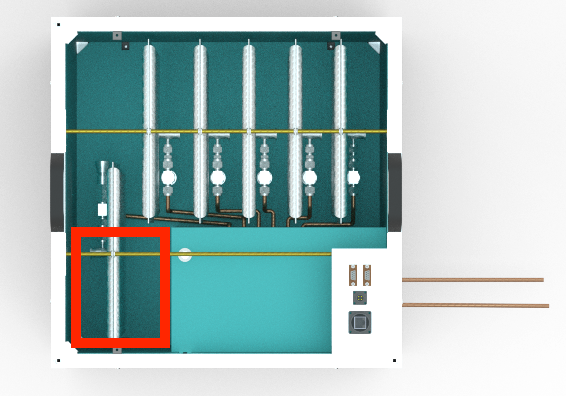
\includegraphics[width=0.8\textwidth]{4-experiment-design/img/Mechanical/Figure_15.png}
    \caption{\DIFaddFL{Layout Including a Battery (in Red).}}
    \label{battery_distribution}
\end{figure}

\pagebreak
\DIFaddend Since the CAC \DIFdelbegin \DIFdel{will be }\DIFdelend \DIFaddbegin \DIFadd{was }\DIFaddend the heaviest component in the whole experiment its positioning and orientation inside the gondola \DIFdelbegin \DIFdel{will directly affect }\DIFdelend \DIFaddbegin \DIFadd{directly affected }\DIFaddend the stress analysis of the structure. In the worst case scenario, without a proper study of the aforesaid interface, shear in the screws could be produced after a violent landing stress or unexpected shaking. The larger the distance to the fixed points, the bigger the momentum produced by the component. For this reason, the CAC box \DIFdelbegin \DIFdel{will be }\DIFdelend \DIFaddbegin \DIFadd{was }\DIFaddend securely attached to the AAC box by means of six anchor points with four screws each. This fixing interface can be seen in red in Figure \ref{dimensions} to help the fast recovery. Taking into account also the two extra anchor points to the gondola, the fast recovery of CAC then \DIFdelbegin \DIFdel{will only require }\DIFdelend \DIFaddbegin \DIFadd{only required }\DIFaddend unscrewing $16$ screws and unplugging a D-Sub connector.

 \begin{figure}[H]
     \centering
     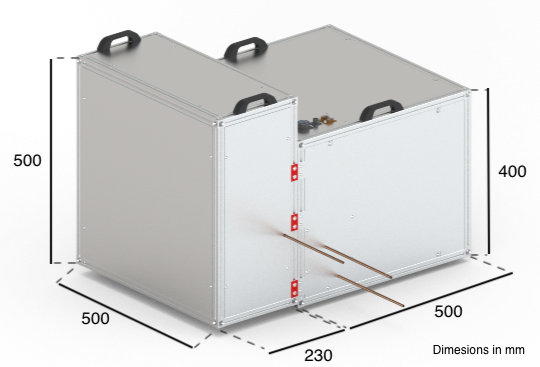
\includegraphics[width=0.9\textwidth]{4-experiment-design/img/Mechanical/Figure_14.png}
     \caption{General Dimensions of the Experiment.}
     \label{dimensions}
\end{figure}



\DIFdelbegin %DIFDELCMD < \begin{figure}[H]
%DIFDELCMD <     \centering
%DIFDELCMD <     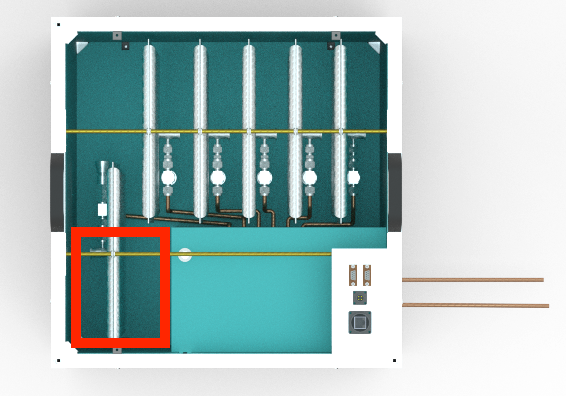
\includegraphics[width=0.45\textwidth]{4-experiment-design/img/Mechanical/Figure_15.png}
%DIFDELCMD <     %%%
%DIFDELCMD < \caption{%
{%DIFAUXCMD
\DIFdelFL{Layout Including a Battery (in Red).}}
    %DIFAUXCMD
%DIFDELCMD < \label{battery_distribution}
%DIFDELCMD < \end{figure}
%DIFDELCMD < 

%DIFDELCMD < %%%
\DIFdelend The main mechanical characteristics of the experiment are summarized in Table \ref{table:experiment-summary}, where the values are based on the reference axis shown in Figure \ref{COG}. The Center Of Gravity for the whole experiment \DIFdelbegin \DIFdel{is }\DIFdelend \DIFaddbegin \DIFadd{was }\DIFaddend determined to be located just on the plate of the third level of the Brain, which coincides with the location of the electronics PCB. This outcome \DIFdelbegin \DIFdel{is }\DIFdelend \DIFaddbegin \DIFadd{was }\DIFaddend quite advantageous in terms of stability for one of the most sensitive subsystems of the experiment in terms of shakes and loads. 
%DIF < It should also be noted that the weights of the table for the boxes and, therefore, the whole experiment, are increased by a safety margin of $10\%$.

\begin{table}[H]
\noindent\makebox[\columnwidth]{%
\scalebox{0.8}{
\begin{tabular}{c|c|c|c|}
\cline{2-4}
 & CAC & AAC & TOTAL \\ \hline
\multicolumn{1}{|c|}{Experiment mass {[}kg{]}} & $11.95$ & $12.21$ & $24.16$ \\ \hline
\multicolumn{1}{|c|}{Experiment dimensions {[}m{]}} & $0.23\times0.5\times0.5$ & $0.5\times0.5\times0.4$ & $0.73\times0.5\times0.5$ \\ \hline
\multicolumn{1}{|c|}{Experiment footprint area {[}$m^2${]}} & $0.115$ & $0.25$ & $0.365$ \\ \hline
\multicolumn{1}{|c|}{Experiment volume {[}$m^3${]}} & $0.0575$ & $0.1$ & $0.1575$ \\ \hline
\multicolumn{1}{|c|}{Experiment expected COG position} & \begin{tabular}[c]{@{}l@{}}$X=23.51\ cm$\\ $Y=10\ cm$\\ $Z=22.57\ cm$ \end{tabular}  & \begin{tabular}[c]{@{}l@{}} $X=29.04\ cm$\\ $Y=16.63\ cm$\\  $Z=16.2\ cm$ \end{tabular} &\begin{tabular}[c]{@{}l@{}} $X=26.31\ cm$\\ $Y=24.99\ cm$\\  $Z=19.35\ cm$  \end{tabular} \\ \hline
\end{tabular}}}
\caption{Experiment Summary Table.}
\label{table:experiment-summary}
\end{table}


 \begin{figure}[H]
     \centering
     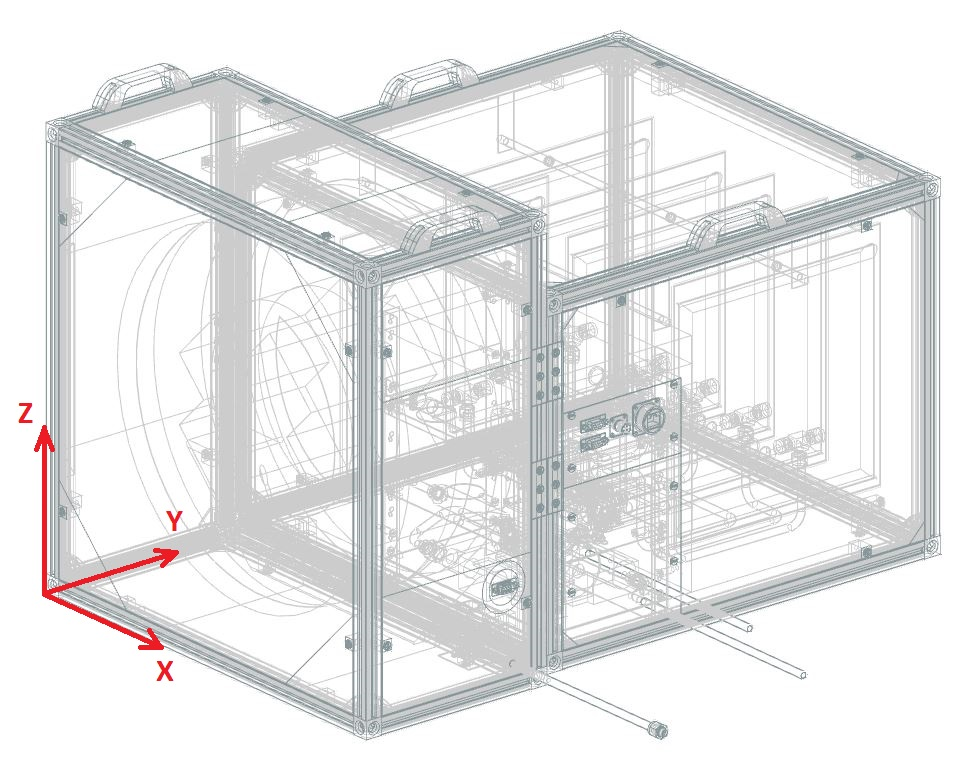
\includegraphics[width=0.45\textwidth]{4-experiment-design/img/Mechanical/COG.jpg}
     \caption{Reference Axis for the Total Center of Gravity.}
     \label{COG}
\end{figure}

\pagebreak
\subsubsection{Structure}
\label{sec:4.4.1}

The main purpose of \DIFdelbegin \DIFdel{an }\DIFdelend \DIFaddbegin \DIFadd{the }\DIFaddend experiment box structure \DIFdelbegin \DIFdel{is }\DIFdelend \DIFaddbegin \DIFadd{was }\DIFaddend to provide overall mechanical integrity and maintain the system geometry. It \DIFdelbegin \DIFdel{is }\DIFdelend \DIFaddbegin \DIFadd{was }\DIFaddend able to carry the loads of all the phases of the flight and ensure that all the components and subsystems \DIFdelbegin \DIFdel{can }\DIFdelend \DIFaddbegin \DIFadd{could }\DIFaddend withstand them. Test 9 in Table \ref{tab:vibration-test} helped to confirm the frame \DIFdelbegin \DIFdel{can }\DIFdelend \DIFaddbegin \DIFadd{could }\DIFaddend withstand these vibrations.

Moreover, other considerations such as electrical and, especially, thermal conductivity \DIFdelbegin \DIFdel{are }\DIFdelend \DIFaddbegin \DIFadd{were }\DIFaddend also a concern since the experiment \DIFdelbegin \DIFdel{will fly }\DIFdelend \DIFaddbegin \DIFadd{flown }\DIFaddend up to $25\ km$ in the Polar Circle \DIFdelbegin \DIFdel{in mid October }\DIFdelend and many critical subsystems \DIFdelbegin \DIFdel{have }\DIFdelend \DIFaddbegin \DIFadd{had }\DIFaddend tight operative ranges values.

 \begin{figure}[H]
     \centering
     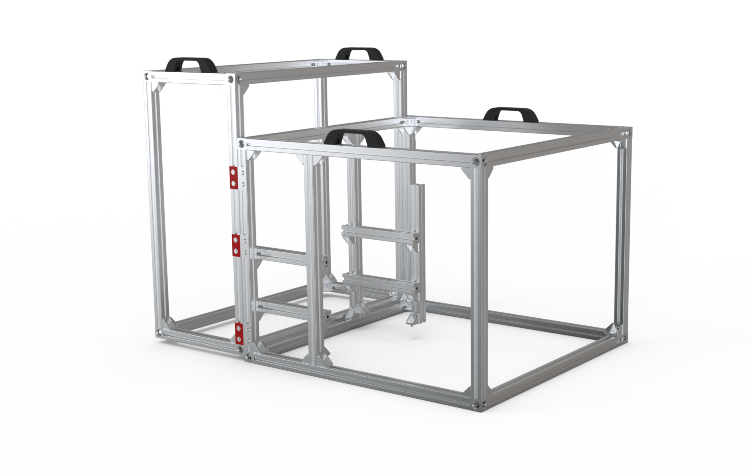
\includegraphics[width=0.8\textwidth]{4-experiment-design/img/Mechanical/structure.png}
     \caption{Structure Overview.}
     \label{fig:structure}
\end{figure}

For this purpose, two boxes built with straight frames \DIFdelbegin \DIFdel{have been }\DIFdelend \DIFaddbegin \DIFadd{were }\DIFaddend chosen as the best option as shown in Figure \ref{fig:structure}. The frame of these boxes \DIFdelbegin \DIFdel{are }\DIFdelend \DIFaddbegin \DIFadd{were }\DIFaddend strut profiles made of aluminum, with a characteristic cross-section of $20\times20\ mm$, and with $M6$ thread at each side. The rails \DIFdelbegin \DIFdel{allow }\DIFdelend \DIFaddbegin \DIFadd{allowed }\DIFaddend an easy interface between bars and other elements. In turn, these profiles \DIFdelbegin \DIFdel{are }\DIFdelend \DIFaddbegin \DIFadd{were }\DIFaddend joined together in each corner with aluminum cubic connectors of $20\times20\ mm$ (see Figure \ref{fig:corner_cube}) and $M6\times16$ bolts aligned with the bars axis. At the same time, these nodes \DIFdelbegin \DIFdel{have been }\DIFdelend \DIFaddbegin \DIFadd{were }\DIFaddend reinforced by three $20/20$ brackets (see Figure \ref{fig:corner_bracket}), each \DIFdelbegin \DIFdel{is }\DIFdelend \DIFaddbegin \DIFadd{was }\DIFaddend fixed to the frames with $M4\times8$ bolts and the corresponding $M4$ T-nut. All these components were manufactured by Bosch Rexroth.

\bigskip
\begin{figure}[H]
    \noindent\makebox[\textwidth]{%
    \begin{subfigure}{.35\textwidth}
        \centering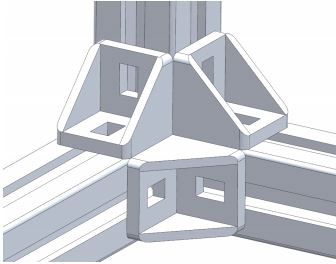
\includegraphics[width=1\textwidth]{4-experiment-design/img/Mechanical/corner_brackets.jpg}
        \caption{Brackets Reinforcement.}
        \label{fig:corner_bracket}
    \end{subfigure}
    \hspace{1cm}
    \begin{subfigure}{.35\textwidth}
        \centering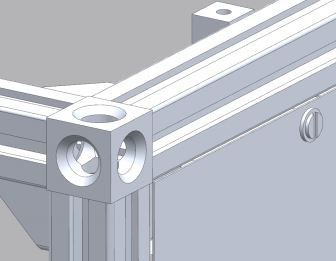
\includegraphics[width=1\textwidth] {4-experiment-design/img/Mechanical/corner_cube.jpg}
        \caption{Cubic Connector.}
        \label{fig:corner_cube}
    \end{subfigure}}
    \caption{Strut Profiles Connections.}
    \label{fig:profile_connection}
\end{figure}

\bigskip
Table \ref{table:profile_momentum} shows the main mechanical properties of the Bosch Rexroth $20/20$ strut profiles used in the structure. For further details see Table \ref{table:profile_material}.


\begin{longtable}{|m{0.2\textwidth}|m{0.14\textwidth}|m{0.25\textwidth}|m{0.3\textwidth}|}
\hline
\textbf{Section surface} & \textbf{Mass} & \textbf{Moment of Inertia ($I_x = I_y$)} & \textbf{Moment of resistance ($W_x = W_y$)} \\ \hline 
$1.6\ cm^2$ & $0.4\ kg/m$ & $0.7\ cm^4$ & $0.7\ cm^3$ \\ \hline

\caption{Intrinsic Characteristics of the Strut Profiles.}
\label{table:profile_momentum}
\end{longtable}

\smallskip

\subsubsection{Walls and Protections}
\label{sec:4.4.2}

Since the experiment \DIFdelbegin \DIFdel{will be }\DIFdelend \DIFaddbegin \DIFadd{was }\DIFaddend placed close to the outside of the gondola, it \DIFdelbegin \DIFdel{is }\DIFdelend \DIFaddbegin \DIFadd{was }\DIFaddend very exposed to both external elements impacts and also possible broken parts from other experiments in the gondola due to unexpected rapid movements, and a probable hard landing impact. Therefore, the experiment box \DIFdelbegin \DIFdel{is }\DIFdelend \DIFaddbegin \DIFadd{was }\DIFaddend shielded with removable aluminum walls along with a thick layer of Styrofoam attached to each wall. This thickness \DIFdelbegin \DIFdel{varies }\DIFdelend \DIFaddbegin \DIFadd{varied }\DIFaddend from two to three centimeters in the AAC box, and five centimeters to protect the AirCore. Besides protection, the thickness of the styrofoam \DIFdelbegin \DIFdel{is }\DIFdelend \DIFaddbegin \DIFadd{was }\DIFaddend also motivated by thermal control issues.
% which is explained more in detail in Section \ref{sec:4.6.6}.

To mount the experiment a combination of three different elements \DIFdelbegin \DIFdel{are }\DIFdelend \DIFaddbegin \DIFadd{were }\DIFaddend used, as shown in Figure \ref{fig:wall_attach}. The walls \DIFdelbegin \DIFdel{are }\DIFdelend \DIFaddbegin \DIFadd{were }\DIFaddend screwed to the Variofix blocks by means of $M4\times8$ bolts. In between the aluminum walls and the bolts, a $M4$ retainer ring \DIFdelbegin \DIFdel{has been }\DIFdelend \DIFaddbegin \DIFadd{was }\DIFaddend placed to improve the fixation of each spot. Eight fixation points for each wall \DIFdelbegin \DIFdel{have been }\DIFdelend \DIFaddbegin \DIFadd{were }\DIFaddend considered sufficient to keep the experiment safe from any impact.

The styrofoam sheets \DIFdelbegin \DIFdel{are }\DIFdelend \DIFaddbegin \DIFadd{were }\DIFaddend attached to the aluminum walls with double sided tape.

Tables \ref{table:wall_aluminum} and \ref{table:wall_styrofoam} show the main properties of the materials used to build the walls of the boxes.

 \begin{figure}[H]
     \centering
     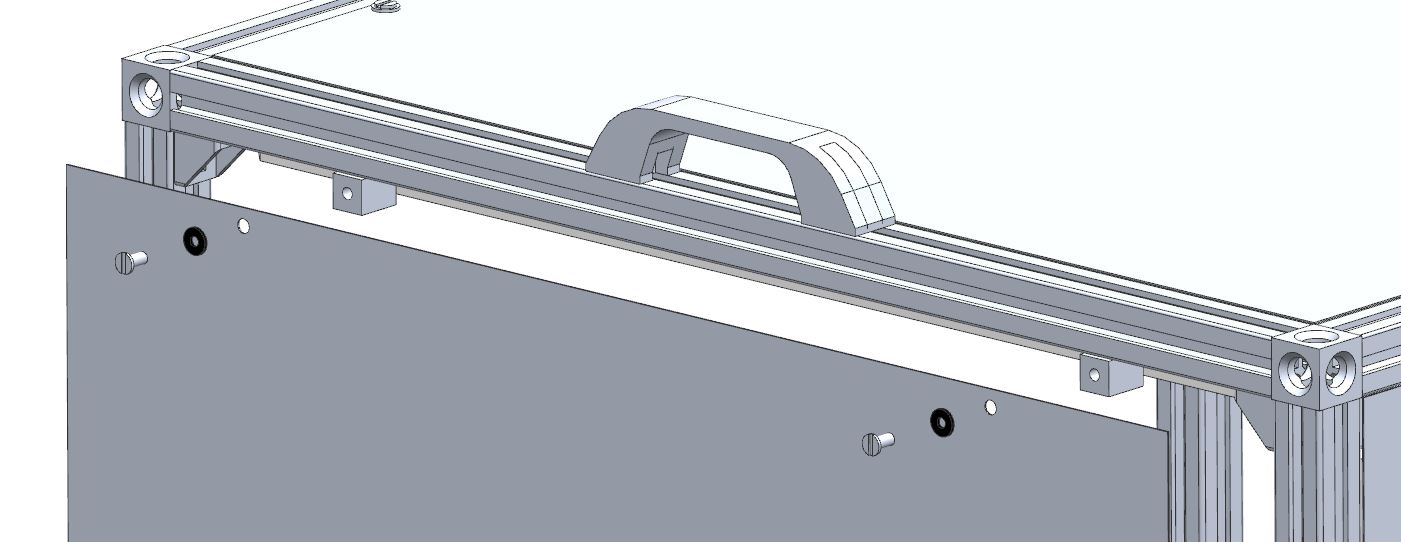
\includegraphics[width=0.5\textwidth]{4-experiment-design/img/Mechanical/wall_attachment.jpg}
     \caption{Exploit View of the Attachment of the Walls.}
     \label{fig:wall_attach}
\end{figure}

\subsubsection{CAC Box}

The CAC subsystem \DIFdelbegin \DIFdel{is }\DIFdelend \DIFaddbegin \DIFadd{was }\DIFaddend designed to fit a $300$ m stainless steel coiled tube, a solenoid valve provided by SMC controlling it, tube fittings manufactured by Swagelok, an air filter and three temperature sensors. A schematic of this subsystem can be seen in Figure \ref{fig:CAC-schematic}. The CAC \DIFdelbegin \DIFdel{consists }\DIFdelend \DIFaddbegin \DIFadd{consisted }\DIFaddend of a combination of a $200$ m coiled tube of $1/8$ inches diameter and a $100$ m coiled tube of $1/4$ inches diameter. The outlet of the CAC \DIFdelbegin \DIFdel{is }\DIFdelend \DIFaddbegin \DIFadd{was }\DIFaddend sealed with a quick connector provided by FMI. The inlet \DIFdelbegin \DIFdel{is }\DIFdelend \DIFaddbegin \DIFadd{was }\DIFaddend sealed the same way but it \DIFdelbegin \DIFdel{can }\DIFdelend \DIFaddbegin \DIFadd{could }\DIFaddend be opened by another interface plugged into the quick connector. A custom made filter by FMI \DIFdelbegin \DIFdel{is }\DIFdelend \DIFaddbegin \DIFadd{was }\DIFaddend placed between this orifice and the solenoid valve. The filter \DIFdelbegin \DIFdel{contains }\DIFdelend \DIFaddbegin \DIFadd{contained }\DIFaddend magnesium perchlorate powder with stone wool at both ends of the tube. It \DIFdelbegin \DIFdel{ensures }\DIFdelend \DIFaddbegin \DIFadd{ensured }\DIFaddend that no moisture \DIFdelbegin \DIFdel{will enter }\DIFdelend \DIFaddbegin \DIFadd{entered }\DIFaddend the coil during any testing or sampling. A piece of stainless steel tube, manufactured by Silcotek, \DIFdelbegin \DIFdel{is }\DIFdelend \DIFaddbegin \DIFadd{was }\DIFaddend attached to the solenoid valve that goes outside the box, thus having a direct outside outlet and inlet for the whole CAC system, as seen in Figure \ref{fig:CAC-cad-model}.

A D-sub cable \DIFdelbegin \DIFdel{will be }\DIFdelend \DIFaddbegin \DIFadd{was }\DIFaddend used to connect the electrical components to the control unit in the AAC box. Both boxes \DIFdelbegin \DIFdel{have }\DIFdelend \DIFaddbegin \DIFadd{had }\DIFaddend their own D-sub connector, which \DIFdelbegin \DIFdel{is }\DIFdelend \DIFaddbegin \DIFadd{was }\DIFaddend located on one of the box's walls.

% mechanical issues and gondola constraints 

\begin{figure}[H]
    \centering
    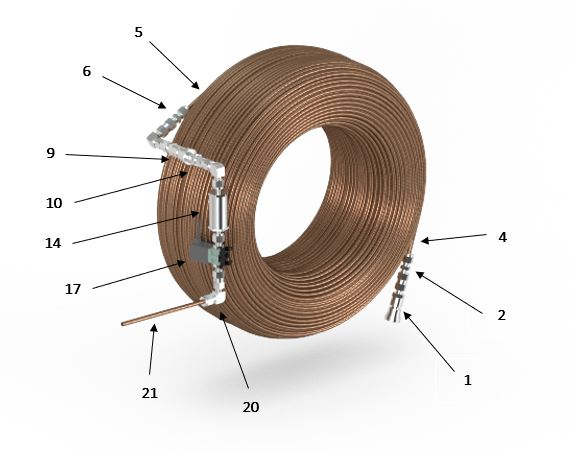
\includegraphics[width=0.6\textwidth]{4-experiment-design/img/Mechanical/CAC_labels.jpg}
    \caption{3D Model of the Aircore and its pneumatic fittings. The Numbers Correspond to the main components in Figure. \ref{fig:CAC-schematic}.}
    \label{fig:CAC-cad-model}
\end{figure}

\begin{landscape}
\begin{figure}[H]
    \centering
    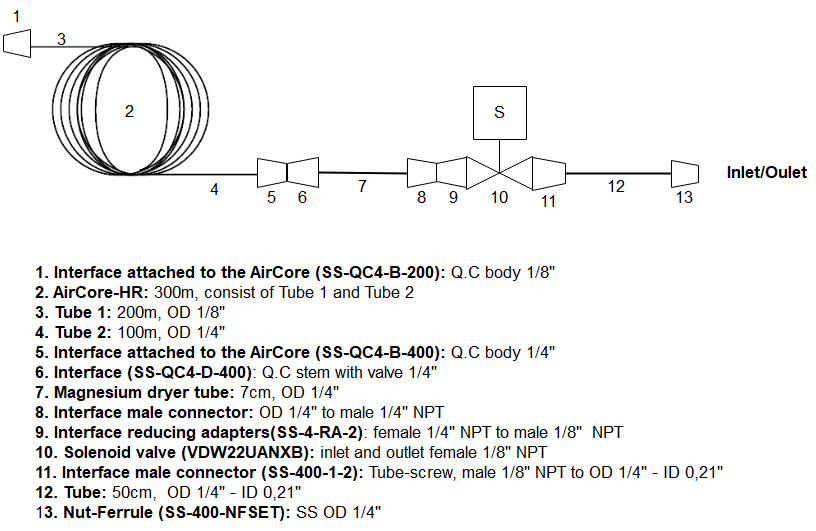
\includegraphics[width=1.3\textwidth]{4-experiment-design/img/Mechanical/CAC-schematic.PNG}
    \caption{Schematic of CAC.}
    \label{fig:CAC-schematic}
\end{figure}
\end{landscape}
\smallskip

\pagebreak
\subsubsection{AAC Box}\label{sec:aac-analysis}
The AAC box has been designed and manufactured to be as compact as possible. An analysis regarding the variation of the bags dimensions to different sampled volume, was made and is summarized in Appendix \ref{dimensions-bags}. From these results it was shown that the AAC subsystem \DIFdelbegin \DIFdel{is }\DIFdelend \DIFaddbegin \DIFadd{was }\DIFaddend able to fit six $3\ L$ sampling bags, provided by RESTEK, together with The Brain that \DIFdelbegin \DIFdel{includes }\DIFdelend \DIFaddbegin \DIFadd{included }\DIFaddend the pneumatic system and the electronic box. Each bag \DIFdelbegin \DIFdel{has }\DIFdelend \DIFaddbegin \DIFadd{had }\DIFaddend a dedicated valve in the Valve Center (VC) to allow emptying and filling processes as well as to close the bag when needed. The bags \DIFdelbegin \DIFdel{hang }\DIFdelend \DIFaddbegin \DIFadd{hung }\DIFaddend from a bar that \DIFdelbegin \DIFdel{is }\DIFdelend \DIFaddbegin \DIFadd{was }\DIFaddend attached to the structure frame by two anchor points on the top. The distribution layout can be seen in Figures \ref{iso_aac} and \ref{lateral_aac}. To ensure a properly built pneumatic system with the minimal leakage risk, all tubes manufactured by Silcotek in the system were exclusively connected to tube fittings which were provided by Swagelok. 


%DIF < The AAC Subsystem consists of six $3\ L$ sampling bags. Each bag will have a dedicated valve in the Valve Center (VC) to allow emptying and filling processes as well as to close the bag when needed. The bags will be placed vertically and will have two anchor points: on the top through a  multiple anchor interface (see Figure \ref{anchor_bags}) and on the bottom by means of the tubes connecting them to the valves.
\DIFdelbegin %DIFDELCMD < 

%DIFDELCMD < %%%
%DIF < % Several Figures of the top box with its inside elements: isometric, top view and front view.
%DIFDELCMD < 

%DIFDELCMD < %%%
%DIF < \begin{figure}[H]
%DIF <     \centering
%DIF <     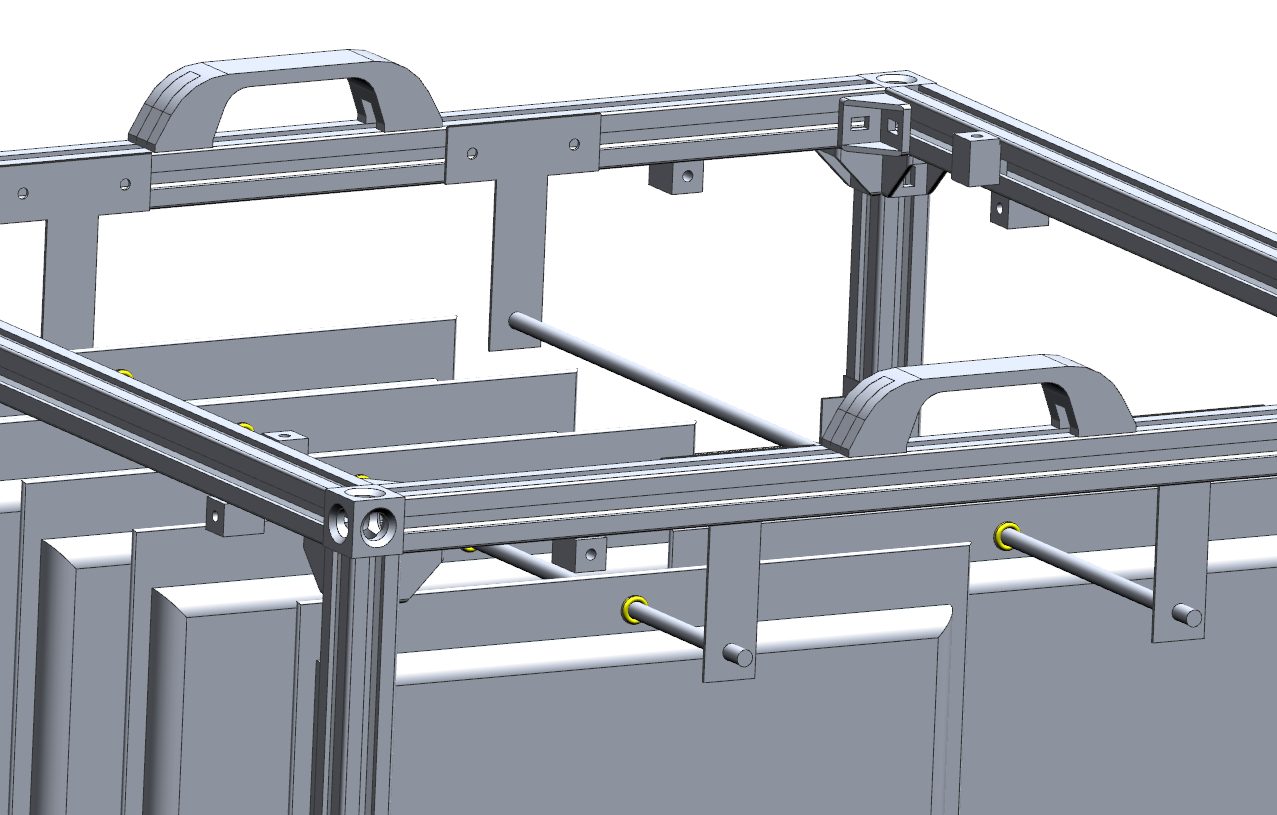
\includegraphics[width=0.6\textwidth]{4-experiment-design/img/Mechanical/Bags_Fixing_Interface.png}
%DIF <     \caption{Sampling Bags with Fixing Interface and the AAC Box Handles.}
%DIF <     \label{anchor_bags}
%DIF < \end{figure}
%DIFDELCMD < 

%DIFDELCMD < %%%
%DIF < \underline{Distribution}
%DIFDELCMD < 

%DIFDELCMD < %%%
%DIF < The AAC box has been designed to be as compact as possible, which was a challenging iterative process since the bags dimensions vary during the flight. The process led to a square base box that is able to fit six sampling bags together with a control center called The Brain that includes the pneumatic system and the electronic box. The distribution layout can be seen in Figures \ref{iso_aac} and \ref{lateral_aac}.
%DIFDELCMD < 

%DIFDELCMD < %%%
%DIF <  Figure: Top view to show the distribution of the AAC Box
%DIFDELCMD < 

%DIFDELCMD < %%%
\DIFdelend \begin{figure}[H]
    \centering
    \begin{subfigure}[b]{0.47\textwidth}
        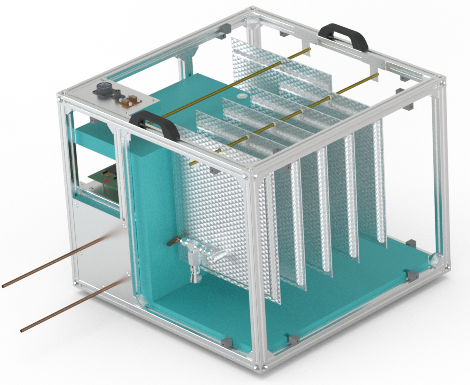
\includegraphics[width=\textwidth]{4-experiment-design/img/Mechanical/Figure_22a.png}
         \caption{Isometric View of the AAC Box.}
    \label{iso_aac}
    \end{subfigure}
    ~
    \begin{subfigure}[b]{0.47\textwidth}
        \centering
         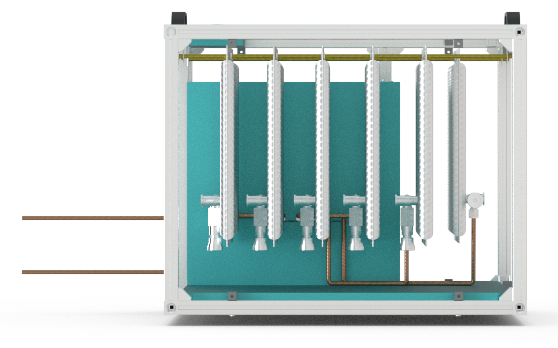
\includegraphics[width=\textwidth]{4-experiment-design/img/Mechanical/Figure_22b.png}
        \caption{Lateral View of the AAC Box.}
        \label{lateral_aac}
        \end{subfigure}
    \caption{Distribution Inside the AAC Box.}
    \label{fig:Distribution-AAC}
\end{figure}


%DIF < \begin{figure}[H]
%DIF <     \centering
%DIF <     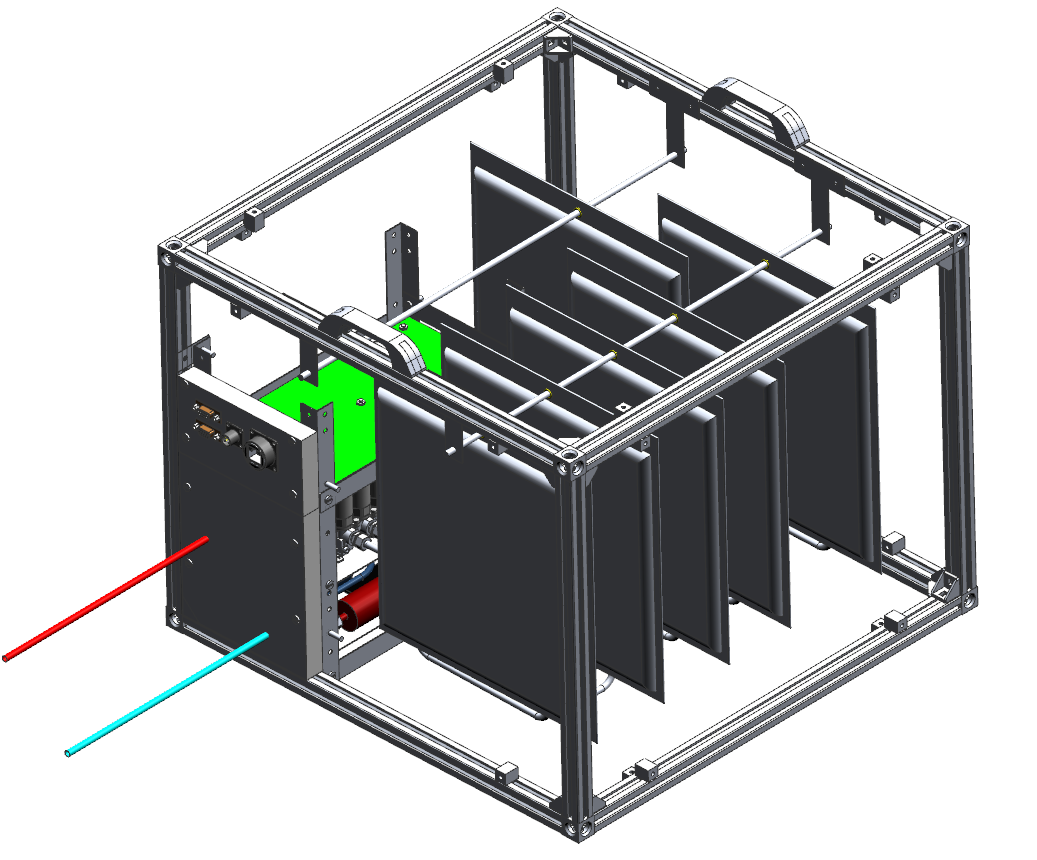
\includegraphics[width=0.6\textwidth]{4-experiment-design/img/Mechanical/AAC_isometric_view.png}
%DIF <     \caption{Isometric View of the AAC Box.}
%DIF <     \label{iso_aac}
%DIF < \end{figure}
\DIFdelbegin %DIFDELCMD < 

%DIFDELCMD < %%%
%DIF < %\begin{figure}[H]
%DIF <     \centering
%DIF <     \includegraphics[width=0.6\textwidth]{4-experiment-design/img/Mechanical/AAC_lateral_view.png}
%DIF <     \caption{Lateral View of the AAC Box.}
%DIF <     \label{lateral_aac}
%DIF < \end{figure}
%DIFDELCMD < 

%DIFDELCMD < %%%
%DIF < \begin{figure}[H]
%DIF <     \centering
%DIF <     \includegraphics[width=0.7\textwidth]{4-experiment-design/img/Mechanical/AAC_front_view.png}
%DIF <     \caption{Front View of the AAC Box.}
%DIF <     \label{front_aac}
%DIF < \end{figure}
\DIFdel{In order to reach to all the bags from the Valve Center, the tubes have been properly sized }\DIFdelend \DIFaddbegin \DIFadd{The tubes going from the valve centre to the bags were sized as short as possible }\DIFaddend following science concerns regarding length.  
%DIF < Since the AAC box is expected to be handed over to FMI, the design also takes into consideration the possibility to include a battery for power supply. This would be allocated next to The Brain and imply reducing the sampling bags down to five, see Figure \ref{battery_distribution}.


%DIF <  Figure with a a top view without the 6th bag and with a red box simulating the battery
\DIFdelbegin %DIFDELCMD < 

%DIFDELCMD < %%%
\DIFdelend \pagebreak
\underline{The Brain}
\label{subsec:brain}

\smallskip
The Brain \DIFdelbegin \DIFdel{is }\DIFdelend \DIFaddbegin \DIFadd{was }\DIFaddend an essential part of the experiment. It \DIFdelbegin \DIFdel{is }\DIFdelend \DIFaddbegin \DIFadd{was }\DIFaddend a three-level structure containing both the pneumatic system and the electronics of the experiment, seen in Figure \ref{brain_isometric_open}. Its design \DIFdelbegin \DIFdel{aimed to make }\DIFdelend \DIFaddbegin \DIFadd{made }\DIFaddend it compact enough to both allow a proper thermal control and to fit into the space left next to the sampling bags. It \DIFdelbegin \DIFdel{is }\DIFdelend \DIFaddbegin \DIFadd{was }\DIFaddend placed in a corner of the AAC box. Therefore, The Brain \DIFdelbegin \DIFdel{takes }\DIFdelend \DIFaddbegin \DIFadd{took }\DIFaddend advantage of the vertical space inside the AAC box. It \DIFdelbegin \DIFdel{has }\DIFdelend \DIFaddbegin \DIFadd{had }\DIFaddend three different levels: Level 1 - Pump, Level 2 - Valve Center, and Level 3 - Electronics.


\begin{figure}[H]
    \centering
    \includegraphics[width=0.7\textwidth]{4-experiment-design/img/Mechanical/Figure_23.png}
    \caption{Inside view of The Brain.}
    \label{brain_isometric_open}
\end{figure}
\DIFaddbegin 

\DIFaddend Level 1 of The Brain \DIFdelbegin \DIFdel{is }\DIFdelend \DIFaddbegin \DIFadd{was }\DIFaddend lying on the base wall styrofoam. It \DIFdelbegin \DIFdel{contains }\DIFdelend \DIFaddbegin \DIFadd{contained }\DIFaddend the beginning of the pneumatic sampling system. The inlet tube \DIFdelbegin \DIFdel{passes }\DIFdelend \DIFaddbegin \DIFadd{passed }\DIFaddend through the wall and \DIFdelbegin \DIFdel{interfaces }\DIFdelend \DIFaddbegin \DIFadd{interfaced }\DIFaddend with the filter. From here the system \DIFdelbegin \DIFdel{continues }\DIFdelend \DIFaddbegin \DIFadd{continued }\DIFaddend through the pump provided by KNF, and to Level 2. The reason for having the pump in Level 1 \DIFdelbegin \DIFdel{is }\DIFdelend \DIFaddbegin \DIFadd{was }\DIFaddend to have the minimum vibration transmitted to the other components. As explained in section \ref{subsec:vibration}, a piece of styrofoam \DIFdelbegin \DIFdel{has been }\DIFdelend \DIFaddbegin \DIFadd{was }\DIFaddend added between the pump and the level 1 plate to help mitigate its vibrations. The pump \DIFdelbegin \DIFdel{has two heaters close by that will be }\DIFdelend \DIFaddbegin \DIFadd{had two heaters on it that were }\DIFaddend used to regulate its temperature. %This can be seen as two black rectangular sheets underneath the pump in Figure \ref{level_1}.

The second level of The Brain \DIFdelbegin \DIFdel{is }\DIFdelend \DIFaddbegin \DIFadd{was }\DIFaddend responsible for the distribution of the air to the selected sampling bag. From Level 1, the air \DIFdelbegin \DIFdel{passes }\DIFdelend \DIFaddbegin \DIFadd{passed }\DIFaddend through the airflow sensor and the static pressure sensor that \DIFdelbegin \DIFdel{allow }\DIFdelend \DIFaddbegin \DIFadd{allowed }\DIFaddend for monitoring the behavior of the system. The manifold with six solenoid valves, manufactured by SMC, \DIFdelbegin \DIFdel{is }\DIFdelend \DIFaddbegin \DIFadd{was }\DIFaddend the main component. From here, the tubes \DIFdelbegin \DIFdel{connect }\DIFdelend \DIFaddbegin \DIFadd{were connected }\DIFaddend with the bags. A T-Union connection \DIFdelbegin \DIFdel{is }\DIFdelend \DIFaddbegin \DIFadd{was }\DIFaddend used just before the bag valve. This interface \DIFdelbegin \DIFdel{allows }\DIFdelend \DIFaddbegin \DIFadd{allowed }\DIFaddend the pre-flight flushing of the tubes connecting with the valves as \DIFaddbegin \DIFadd{well as the post-flight analysis as }\DIFaddend explained previously. 

\smallskip
The flushing valve \DIFdelbegin \DIFdel{is }\DIFdelend \DIFaddbegin \DIFadd{was }\DIFaddend responsible to ensure a proper flushing of the system before each sampling period. From the flushing valve, an outlet tube \DIFdelbegin \DIFdel{reaches }\DIFdelend \DIFaddbegin \DIFadd{reached }\DIFaddend the outside environment. This can be seen in Figure \ref{level_2}.

The OBC and its external elements \DIFdelbegin \DIFdel{are }\DIFdelend \DIFaddbegin \DIFadd{were }\DIFaddend allocated in the third level of The Brain. The PCB \DIFdelbegin \DIFdel{is }\DIFdelend \DIFaddbegin \DIFadd{was }\DIFaddend fixed to the aluminum plate by means of 10 standoffs. As shown in Figure \ref{level_3}, it \DIFdelbegin \DIFdel{has }\DIFdelend \DIFaddbegin \DIFadd{had }\DIFaddend a hole, as well as the level plate, to collect all the wires connecting with levels 1 and 2. This level \DIFdelbegin \DIFdel{has }\DIFdelend \DIFaddbegin \DIFadd{had }\DIFaddend its own outside top wall which \DIFdelbegin \DIFdel{contains }\DIFdelend \DIFaddbegin \DIFadd{contained }\DIFaddend the electrical interfaces. The latter \DIFdelbegin \DIFdel{allows }\DIFdelend \DIFaddbegin \DIFadd{allowed }\DIFaddend the wall to be opened without having to remove all the sockets attached with screws and a female in the inside of the wall. The styrofoam shielding of The Brain \DIFdelbegin \DIFdel{has }\DIFdelend \DIFaddbegin \DIFadd{had }\DIFaddend a hole on top to allow the temperature sensors wires to reach the inside of the AAC Box. 

A more detailed content of the components for each level is summarized in Appendix \ref{list-of-components-brain}.
\begin{figure}[H]
    \centering
    \begin{subfigure}[b]{0.3\textwidth}
    \centering
    \includegraphics[width=\textwidth]{4-experiment-design/img/Mechanical/Figure_24a.png}
    \caption{Isometric View of Level 1.}
    \label{level_1}
    \end{subfigure}
    ~
    \begin{subfigure}[b]{0.3\textwidth}
    \centering
    \includegraphics[width=\textwidth]{4-experiment-design/img/Mechanical/Figure_24b.png}
    \caption{Isometric View of Level 2.}
    \label{level_2}
    \end{subfigure}
    ~
    \begin{subfigure}[b]{0.3\textwidth}
    \centering
    \includegraphics[width=0.8\textwidth]{4-experiment-design/img/Mechanical/Figure_24c.png}
    \caption{Isometric View of Level 3.}
    \label{level_3}
    \end{subfigure}
    \caption{Distribution in Each Level.}
    \label{fig:The-brain}
\end{figure}
%DIF < Level 1 is the base of the AAC box and together with Level 2 contain the main pneumatic system. This is commanded by the electronics in the top level. This distribution allows easy access to the PCB from the top and provides the physical desired separation between electronics and pneumatic circuit. 


This distribution \DIFdelbegin \DIFdel{allows }\DIFdelend \DIFaddbegin \DIFadd{allowed }\DIFaddend easy access to the PCB from the top and \DIFdelbegin \DIFdel{provides }\DIFdelend \DIFaddbegin \DIFadd{provided }\DIFaddend the physical desired separation between electronics and pneumatic circuit.
%DIF < This is shown in the dedicated section for each level which can be seen in Figure \ref{brain_lateral}.


%DIF < \begin{figure}[H]
%DIF <     \centering
%DIF <     \includegraphics[width=0.6\textwidth]{4-experiment-design/img/Mechanical/Brain_Lateral.png}
%DIF <     \caption{Lateral View of The Brain.}
%DIF <     \label{brain_lateral}
%DIF < \end{figure}
\DIFdelbegin %DIFDELCMD < 

%DIFDELCMD < %%%
\DIFdelend \smallskip
The structure of The Brain \DIFdelbegin \DIFdel{provides }\DIFdelend \DIFaddbegin \DIFadd{provided }\DIFaddend versatility in terms of implementation and construction. It \DIFdelbegin \DIFdel{is }\DIFdelend \DIFaddbegin \DIFadd{was }\DIFaddend made out of strut profiles: four bars placed vertically and four bars placed horizontally. The railed bars \DIFdelbegin \DIFdel{allow }\DIFdelend \DIFaddbegin \DIFadd{allowed }\DIFaddend the possibility to fix all the pieces together and to provide the anchor points for the lateral and top styrofoam shield as well as to fix the whole unit to the box structure bars.
%DIF < This is seen in Figure \ref{brain_structure}. 

%DIF <  \begin{figure}[H]
%DIF <      \centering
%DIF <      \begin{subfigure}[b]{0.48\textwidth}
%DIF <      \centering
%DIF <      \includegraphics[width=\textwidth]{4-experiment-design/img/Mechanical/Brain_Structure.png}
%DIF <      \caption{Structure of The Brain.}
%DIF <      \label{brain_structure}
%DIF <      \end{subfigure}
%DIF <      ~
%DIF <      \begin{subfigure}[b]{0.48\textwidth}
%DIF <      \centering
%DIF <      \includegraphics[width=\textwidth]{4-experiment-design/img/Mechanical/Brain_Isometric.png}
%DIF <      \caption{Isometric View of The Brain with Walls.}
%DIF <      \label{brain_isometric}
%DIF <      \end{subfigure}
%DIF <      \caption{Design of The Brain.}
%DIF <      \label{fig:The-brain}
%DIF <  \end{figure}
\DIFdelbegin %DIFDELCMD < 

%DIFDELCMD < %%%
%DIF < \begin{figure}[H]
%DIF <     \centering
%DIF <     \includegraphics[width=0.8\textwidth]{4-experiment-design/img/Mechanical/Brain_Structure.png}
%DIF <     \caption{Structure of The Brain.}
%DIF <     \label{brain_structure}
%DIF < \end{figure}
%DIFDELCMD < 

%DIFDELCMD < %%%
\DIFdelend \smallskip
The bulk dimensions of The Brain \DIFdelbegin \DIFdel{are }\DIFdelend \DIFaddbegin \DIFadd{were }\DIFaddend 260 mm long, 150mm wide and 290 mm high. If the shielding styrofoam walls \DIFdelbegin \DIFdel{are }\DIFdelend \DIFaddbegin \DIFadd{were }\DIFaddend taken into account, the dimensions \DIFdelbegin \DIFdel{are }\DIFdelend \DIFaddbegin \DIFadd{were }\DIFaddend 290 mm long, 180 mm wide and 300 mm high.
Therefore, accounting for the space the column bars \DIFdelbegin \DIFdel{take}\DIFdelend \DIFaddbegin \DIFadd{took}\DIFaddend , each plate \DIFdelbegin \DIFdel{has }\DIFdelend \DIFaddbegin \DIFadd{had }\DIFaddend a surface of 258 mm x 158 mm. The distance between levels \DIFdelbegin \DIFdel{is }\DIFdelend \DIFaddbegin \DIFadd{was }\DIFaddend variable depending on the components dimensions. Level 1 \DIFdelbegin \DIFdel{has a height if }\DIFdelend \DIFaddbegin \DIFadd{had a height of }\DIFaddend 7 cm, Level 2 \DIFdelbegin \DIFdel{has }\DIFdelend \DIFaddbegin \DIFadd{had }\DIFaddend a height of 9 cm and Level 3 \DIFdelbegin \DIFdel{has }\DIFdelend \DIFaddbegin \DIFadd{had }\DIFaddend 8 cm to the top styrofoam shielding. The Brain with styrofoam shielding can be seen in Figure \ref{brain_isometric}.

\begin{figure}[H]
    \centering
    \includegraphics[width=0.6\textwidth]{4-experiment-design/img/Mechanical/Figure_25_0.png}
    \caption{Isometric View of The Brain.}
    \label{brain_isometric}
\end{figure}

\smallskip
In order to allocate the electrical interfaces required (E-Link, Power Supply and D-Sub Connectors) as well as to allow the tubes of the sampling system to reach the outside environment, the outside facing wall and the top wall \DIFdelbegin \DIFdel{are }\DIFdelend \DIFaddbegin \DIFadd{were }\DIFaddend divided in two pieces each.  This \DIFdelbegin \DIFdel{makes }\DIFdelend \DIFaddbegin \DIFadd{made }\DIFaddend it easy to manipulate when having to open the box walls since the little pieces \DIFdelbegin \DIFdel{containing }\DIFdelend \DIFaddbegin \DIFadd{contained }\DIFaddend the interfaces and the tubes holes, \DIFdelbegin \DIFdel{will remain }\DIFdelend \DIFaddbegin \DIFadd{were remained }\DIFaddend attached. The bottom piece covers Level 1 and 2 while the other, which \DIFdelbegin \DIFdel{contains }\DIFdelend \DIFaddbegin \DIFadd{contained }\DIFaddend the electrical connections, \DIFdelbegin \DIFdel{sits }\DIFdelend \DIFaddbegin \DIFadd{sat }\DIFaddend above Level 3. These pieces \DIFdelbegin \DIFdel{have }\DIFdelend \DIFaddbegin \DIFadd{had }\DIFaddend the same layout as the main wall. 



%DIF < \begin{figure}[H]
%DIF <     \centering
%DIF <     \includegraphics[width=0.8\textwidth]{4-experiment-design/img/Mechanical/Level_1.png}
%DIF <     \caption{Isometric View of Level 1.}
%DIF <     \label{level_1}
%DIF < \end{figure}
\DIFdelbegin %DIFDELCMD < 

%DIFDELCMD < %%%
%DIF < \begin{figure}[H]
%DIF <     \centering
%DIF <     \includegraphics[width=0.8\textwidth]{4-experiment-design/img/Mechanical/Level_2.png}
%DIF <     \caption{Isometric View of Level 2.}
%DIF <     \label{level_2}
%DIF < \end{figure}
%DIFDELCMD < 

%DIFDELCMD < %%%
%DIF < \begin{figure}[H]
%DIF <     \centering
%DIF <     \includegraphics[width=0.8\textwidth]{4-experiment-design/img/Mechanical/Level_3.png}
%DIF <     \caption{Isometric View of Level 3.}
%DIF <     \label{level_3}
%DIF < \end{figure}
%DIFDELCMD < 

%DIFDELCMD < %%%
\DIFdelend \bigskip
\underline{Shielding and anchor points}

\smallskip
The most critical components in terms of required thermal control \DIFdelbegin \DIFdel{are }\DIFdelend \DIFaddbegin \DIFadd{were }\DIFaddend inside The Brain. These \DIFdelbegin \DIFdel{are }\DIFdelend \DIFaddbegin \DIFadd{were }\DIFaddend the pump and the valves. In order to provide a passive thermal shielding, 3 cm thick removable styrofoam walls \DIFdelbegin \DIFdel{are }\DIFdelend \DIFaddbegin \DIFadd{were }\DIFaddend placed in the three walls (top, lateral, and rear) facing the interior of the AAC box, shown in Figure \ref{brain_isometric}. The lateral wall \DIFdelbegin \DIFdel{is }\DIFdelend \DIFaddbegin \DIFadd{was }\DIFaddend fixed by means of four bolts that \DIFdelbegin \DIFdel{penetrate }\DIFdelend \DIFaddbegin \DIFadd{penetrated }\DIFaddend inside the styrofoam. The top wall \DIFdelbegin \DIFdel{is }\DIFdelend \DIFaddbegin \DIFadd{was }\DIFaddend fixed to the rear wall and both \DIFdelbegin \DIFdel{are }\DIFdelend \DIFaddbegin \DIFadd{were }\DIFaddend kept in place by means of a stoper. The larger lateral wall, where the tubes from the valves \DIFdelbegin \DIFdel{are, is }\DIFdelend \DIFaddbegin \DIFadd{were, was }\DIFaddend divided in two pieces so it \DIFdelbegin \DIFdel{can }\DIFdelend \DIFaddbegin \DIFadd{could }\DIFaddend be removed without having to disconnect the tubes. 

\smallskip
The Brain structure \DIFdelbegin \DIFdel{is }\DIFdelend \DIFaddbegin \DIFadd{was }\DIFaddend integrated in the AAC box structure to provide the required stiffness to this element. 


%DIF < \begin{figure}[H]
%DIF <     \centering
%DIF <     \includegraphics[width=1\textwidth]{4-experiment-design/img/Mechanical%/Panel_Front.png}
%DIF <     \caption{Front View of The Brain Where the Styrofoam Walls can be Identified.}
%DIF <     \label{brain_front}
%DIF < \end{figure}
\DIFdelbegin %DIFDELCMD < 

%DIFDELCMD < %%%
\DIFdelend \pagebreak
\subsubsection{Pneumatic Subsystem}
\label{sec:4.4.5}

In order to be able to collect separated samples of air, a pneumatic subsystem \DIFdelbegin \DIFdel{has been }\DIFdelend \DIFaddbegin \DIFadd{was }\DIFaddend developed and implemented. The schematics and components of this can be seen in Figure \ref{pneumatic_system}. The system \DIFdelbegin \DIFdel{is }\DIFdelend \DIFaddbegin \DIFadd{was }\DIFaddend formed by almost $100$ components located inside The Brain and the AAC Box. 

In between these components, the same Sulfinert-treated stainless steel tubing as the ones used for the Inlet/Outlet pipes explained in Section \ref{subsec:pipes} \DIFdelbegin \DIFdel{have been chosen. 
%DIF < According to the datasheet, the minimum suggested bend radius for the chosen diameter tube is $10.2\ cm$. Any bend sharper than this may cause the tubing to stretch, potentially creating active sites as the coating layer density decreases. For this reason, $90^\circ$ elbow interfaces have been used instead of the previously considered straight ones,  to perform all the required sharp curves to allocate all the components inside the volume-limited \emph{Brain}.
}\DIFdelend \DIFaddbegin \DIFadd{were chosen. 
}\DIFaddend 

The schematic for the pneumatic system can be seen in Figure \ref{pneumatic_system}. The air \DIFdelbegin \DIFdel{is }\DIFdelend \DIFaddbegin \DIFadd{was }\DIFaddend sucked from the outside through the inlet tube (No.1), the lower tube in Figure \ref{pneumatic_system_cad}, and it \DIFdelbegin \DIFdel{goes }\DIFdelend \DIFaddbegin \DIFadd{went }\DIFaddend through the filter (No.2) inside the pump (No.9). From here, and changing to Level 2, it \DIFdelbegin \DIFdel{passes }\DIFdelend \DIFaddbegin \DIFadd{passed }\DIFaddend through the airflow sensor (No.15), which \DIFdelbegin \DIFdel{allows }\DIFdelend \DIFaddbegin \DIFadd{allowed }\DIFaddend the airflow rate to be monitored. Thereafter the air \DIFdelbegin \DIFdel{passes }\DIFdelend \DIFaddbegin \DIFadd{passed }\DIFaddend through the static pressure sensor (No.20) before getting to the six station manifold (No.23). It \DIFdelbegin \DIFdel{is }\DIFdelend \DIFaddbegin \DIFadd{was }\DIFaddend in here where the air \DIFdelbegin \DIFdel{is }\DIFdelend \DIFaddbegin \DIFadd{was }\DIFaddend directed to the desired bag (No.36) thanks to its dedicated solenoid valve (No.30).

When flushing the pneumatic system before each sampling period, the flushing valve (No.27) \DIFdelbegin \DIFdel{is }\DIFdelend \DIFaddbegin \DIFadd{was }\DIFaddend opened so that the outlet of the system \DIFdelbegin \DIFdel{is }\DIFdelend \DIFaddbegin \DIFadd{was }\DIFaddend open and new air \DIFdelbegin \DIFdel{runs }\DIFdelend \DIFaddbegin \DIFadd{ran }\DIFaddend through the main part of the pneumatic system. 


%DIF < \begin{figure}[H]
%DIF <     \centering
%DIF <     \begin{subfigure}[b]{0.48\textwidth}
%DIF <     \centering
%DIF <     \includegraphics[width=\textwidth]{4-experiment-design/img/Mechanical/ Pneumatic_System_Top_View_Level_1.png}
%DIF <     \caption{Top View of Level 1.}
%DIF <     \label{level_1_pneumatic_system_top_view}
%DIF <     \end{subfigure}
%DIF <     ~
%DIF <     \begin{subfigure}[b]{0.48\textwidth}
%DIF <     \centering
%DIF <     \includegraphics[width=\textwidth]{4-experiment-design/img/Mechanical/Pneumatic_System_Top_View_Level_2.png}
%DIF <     \caption{Top View of Level 2.}
%DIF <     \label{level_2_pneumatic_system_top_view}
%DIF <     \end{subfigure}
%DIF <     \caption{View Over the Pneumatic System.}
%DIF <     \label{fig:Pneumatic-system}
%DIF < \end{figure}
\DIFdelbegin %DIFDELCMD < 

%DIFDELCMD < %%%
\DIFdelend \begin{figure}[H]
    \centering
   \includegraphics[width=0.8\textwidth]{4-experiment-design/img/Mechanical/Figure_26.png}
   \caption{Pneumatic System Top View.}
    \label{pneumatic_system_cad}
\end{figure}


%DIF < \begin{figure}[H]
%DIF <     \centering
%DIF <     \includegraphics[width=0.8\textwidth]{4-experiment-design/img/Mechanical/Pneumatic_System_Top_View_Level_2.png}
%DIF <     \caption{Pneumatic System Top View of Level 2.}
%DIF <     \label{level_2_pneumatic_system_top_view}
%DIF < \end{figure}
\DIFdelbegin %DIFDELCMD < 

%DIFDELCMD < %%%
%DIF <  Figure with the diagram
%DIFDELCMD < 

%DIFDELCMD < %%%
\DIFdelend \begin{landscape}
\begin{figure}
    \centering
    \includegraphics[width=1.45\textwidth,height=\textheight]{4-experiment-design/img/Mechanical/AAC_System.png}
    \caption{AAC Pneumatic System Diagram and Components.}
    \label{pneumatic_system}
\end{figure}
\end{landscape}

%\raggedbottom
\pagebreak
\subsection{Electrical Design}

\subsubsection{Block Diagram}
\label{sec:4.5.1}

The electronics design can be seen in Figure \ref{fig:electronics-block-diagram} which shows the connections, grounding, voltages, and signals. 

\begin{figure}[H]
    \begin{align*}
        \includegraphics[width=16cm]{4-experiment-design/img/Electrical_Block_diagram.png}
    \end{align*}
    \caption{Block Diagram for all Electronic Components Showing the Connection, Signal and Power Connections.}\label{fig:electronics-block-diagram}
\end{figure}

Most of the electronics \DIFdelbegin \DIFdel{are }\DIFdelend \DIFaddbegin \DIFadd{were }\DIFaddend located in the Brain inside the AAC box. However, there \DIFdelbegin \DIFdel{are }\DIFdelend \DIFaddbegin \DIFadd{were }\DIFaddend six distinct areas:

\begin{enumerate}
    \item The Brain level 3, where the PCB is located with the Arudino and shield, two 24 V DC-DC, two 12 V DC-DC, 11 MOSFETs and 16 LEDs.
    \item The Brain level 2, where the valve manifolds with six sampling valves, the flushing valve, two heaters, airflow sensor, static pressure sensor and one temperature sensor \DIFdelbegin \DIFdel{are }\DIFdelend \DIFaddbegin \DIFadd{were }\DIFaddend located.
    \item The Brain level 1, where the pump, two heaters and one temperature sensor \DIFdelbegin \DIFdel{are }\DIFdelend \DIFaddbegin \DIFadd{were }\DIFaddend located.
    \item The AAC box, where 3 ambient temperature sensors \DIFdelbegin \DIFdel{are }\DIFdelend \DIFaddbegin \DIFadd{were }\DIFaddend located.
    \item The CAC box, where the CAC valve and 3 ambient temperature sensors \DIFdelbegin \DIFdel{are }\DIFdelend \DIFaddbegin \DIFadd{were }\DIFaddend located.
    \item Outside of the experiment box, where 3 ambient pressure sensors \DIFdelbegin \DIFdel{are }\DIFdelend \DIFaddbegin \DIFadd{were }\DIFaddend located.
\end{enumerate}

From the PCB, on level 3, five D-sub connectors \DIFdelbegin \DIFdel{have been }\DIFdelend \DIFaddbegin \DIFadd{were }\DIFaddend used to connect to the other five areas. Fifteen pin connectors \DIFdelbegin \DIFdel{have been }\DIFdelend \DIFaddbegin \DIFadd{were }\DIFaddend used for level 1 and level 2. For the CAC box, AAC box sampling bags area, and the external pressure sensors, nine pin connectors \DIFdelbegin \DIFdel{have been }\DIFdelend \DIFaddbegin \DIFadd{were }\DIFaddend used. In addition there \DIFdelbegin \DIFdel{is }\DIFdelend \DIFaddbegin \DIFadd{was }\DIFaddend a connection to the gondola power and gondola E-link.

All of the power distribution \DIFdelbegin \DIFdel{has been }\DIFdelend \DIFaddbegin \DIFadd{was }\DIFaddend done through the PCB using two 24 V DC-DC and two 12 V DC-DC converters in parallel with a forwarding diode.  
\begin{itemize}
  \item $28.8 \, V \Longrightarrow 24 \, V $ By DC-DC converters
  \item $28.8 \, V \Longrightarrow 12 \, V$ By DC-DC converters
  \end{itemize}
The heaters \DIFdelbegin \DIFdel{do }\DIFdelend \DIFaddbegin \DIFadd{did }\DIFaddend not require the voltage to be stepped down and so \DIFdelbegin \DIFdel{will be }\DIFdelend \DIFaddbegin \DIFadd{were }\DIFaddend powered directly from the gondola battery.

The Arduino \DIFdelbegin \DIFdel{will }\DIFdelend \DIFaddbegin \DIFadd{was used to }\DIFaddend control all of the sensors, valves, heaters and the pump from the PCB. Sensors \DIFdelbegin \DIFdel{have been }\DIFdelend \DIFaddbegin \DIFadd{were }\DIFaddend directly connected to the Arduino. The valves, heaters and the pump \DIFdelbegin \DIFdel{have been }\DIFdelend \DIFaddbegin \DIFadd{were }\DIFaddend connected via a switching circuit.

The LEDs \DIFdelbegin \DIFdel{are }\DIFdelend \DIFaddbegin \DIFadd{were }\DIFaddend used as visual indicators that \DIFdelbegin \DIFdel{display }\DIFdelend \DIFaddbegin \DIFadd{displayed }\DIFaddend whether different parts of the circuit are active or not. They \DIFdelbegin \DIFdel{give }\DIFdelend \DIFaddbegin \DIFadd{gave }\DIFaddend indications on the status of the valves, pump, heaters, DC-DC converters and Arduino. 

Grounding \DIFdelbegin \DIFdel{has been done to follow }\DIFdelend \DIFaddbegin \DIFadd{was done following }\DIFaddend a distributed single point grounding, with all ground connections meeting at a single star point \DIFdelbegin \DIFdel{to ensure there are }\DIFdelend \DIFaddbegin \DIFadd{ensuring there were }\DIFaddend no floating grounds. As not all components \DIFdelbegin \DIFdel{are }\DIFdelend \DIFaddbegin \DIFadd{were }\DIFaddend connected via DC-DC converters the experiment \DIFdelbegin \DIFdel{will not be }\DIFdelend \DIFaddbegin \DIFadd{was not }\DIFaddend isolated from the gondola power supply therefore there \DIFdelbegin \DIFdel{will be }\DIFdelend \DIFaddbegin \DIFadd{was }\DIFaddend a connection between the star point and the gondola ground. The star point \DIFdelbegin \DIFdel{is }\DIFdelend \DIFaddbegin \DIFadd{was }\DIFaddend located on the main PCB board which \DIFdelbegin \DIFdel{is }\DIFdelend \DIFaddbegin \DIFadd{was }\DIFaddend then grounded to the experiment box. The grounding can be seen in Figure \ref{fig:electronics-block-diagram} where it is indicated by dashed lines labeled GND. The analog sensors that \DIFdelbegin \DIFdel{are }\DIFdelend \DIFaddbegin \DIFadd{were }\DIFaddend used on level 1 in the brain \DIFdelbegin \DIFdel{use }\DIFdelend \DIFaddbegin \DIFadd{used }\DIFaddend a separate grounding wire(AGND) onto the main PCB where there \DIFdelbegin \DIFdel{is }\DIFdelend \DIFaddbegin \DIFadd{was }\DIFaddend a separate trace connecting to the ground pins on the Arduino board. Furthermore  the  upper  and  lower  level  of  the  main PCB board \DIFdelbegin \DIFdel{are }\DIFdelend \DIFaddbegin \DIFadd{were }\DIFaddend making use of the common grounding plane where possible.

\subsubsection{Miniature Diaphragm Air Pump}
The pump which \DIFdelbegin \DIFdel{has been selected is }\DIFdelend \DIFaddbegin \DIFadd{was selected was }\DIFaddend the 850.1.2. KNDC B, Figure \ref{fig:pumppic}, which is manufactured by KNF. One of the reasons this pump \DIFdelbegin \DIFdel{has been }\DIFdelend \DIFaddbegin \DIFadd{was }\DIFaddend selected is that it \DIFdelbegin \DIFdel{has successfully been }\DIFdelend \DIFaddbegin \DIFadd{was successfully }\DIFaddend flown on a similar flight in the past where it managed to pump enough air at 25 km altitude to have 180 mL remaining at sea level \cite{LISA}. However, to ensure the pump will operate as intended, several tests \DIFdelbegin \DIFdel{will still be }\DIFdelend \DIFaddbegin \DIFadd{were }\DIFaddend carried out. These tests --- 4, 5, 18, 28 and 29, can be seen in Tables \ref{tab:vacuum-test}, \ref{tab:thermal-test}, \ref{tab:pump-low-pressure-test}, \ref{tab:pump-operation-test}, and \ref{tab:pump-current-pressure-test}.
\DIFdelbegin \DIFdel{The pump has already passed four of these tests and their results can be seen in Appendix \ref{sec:test28result} for Test 28, Appendix \ref{sec:test4results} for test 4, Appendix \ref{subsection:pumplowpressuretest} for Test 18 and Appendix \ref{sec:test29result} for Test 29.
}\DIFdelend 

At sea level conditions the pump was tested and found to have a flow rate of 8.0 L/min and a current draw of 250 mA. The peak current draw was recorded as 600 mA which lasts for less than one second and occurs when the pump is switched on. 

From the results of Test 18, in Section \ref{sec:ExpecterResults}, the flow rate \DIFdelbegin \DIFdel{is }\DIFdelend \DIFaddbegin \DIFadd{was }\DIFaddend shown to be around 3.36 L/min at the lowest pressure that will be seen in flight. This \DIFdelbegin \DIFdel{is }\DIFdelend \DIFaddbegin \DIFadd{was }\DIFaddend in line with requirement D23. The results found in Test 28, in Section \ref{sec:test28result}, \DIFdelbegin \DIFdel{appear }\DIFdelend \DIFaddbegin \DIFadd{appeared }\DIFaddend to be inline with the information given by the manufacturer, seen in Figure \ref{fig:pumpflowcur}.  The highest continuous current draw expected from the pump \DIFdelbegin \DIFdel{is }\DIFdelend \DIFaddbegin \DIFadd{was }\DIFaddend 185 mA when the experiment is at 12 km altitude and \DIFdelbegin \DIFdel{is }\DIFdelend \DIFaddbegin \DIFadd{was }\DIFaddend expected to decrease as we increase in altitude. While it \DIFdelbegin \DIFdel{appears the pump increases }\DIFdelend \DIFaddbegin \DIFadd{appeared that the pump increased }\DIFaddend in current draw at around 6 km there \DIFdelbegin \DIFdel{is }\DIFdelend \DIFaddbegin \DIFadd{was }\DIFaddend no plan to sample below 12 km therefore the highest current draw \DIFdelbegin \DIFdel{can be }\DIFdelend \DIFaddbegin \DIFadd{was }\DIFaddend taken from 12 km. As the pump \DIFdelbegin \DIFdel{has }\DIFdelend \DIFaddbegin \DIFadd{had }\DIFaddend a peak current of 600 mA when it switches on, the mosfet and DC-DC power have been chosen to be able to withstand this demand. 

\begin{figure}[H]
    \begin{align*}
        \includegraphics[width=6cm]{4-experiment-design/img/pump-850-1-2-kndc-b.png}
    \end{align*}
    \caption{KNF 850.1.2. KNDC B Miniature Diaphragm Pump.}\label{fig:pumppic}
\end{figure}


\begin{figure}[H]
    \begin{align*}
        \includegraphics[width=15cm]{4-experiment-design/img/pump-flow-rate-current-graph.png}
    \end{align*}
    \caption{KNF 850.1.2. KNDC B Flow Rate and Current Draw to Pressure Graph.}\label{fig:pumpflowcur}
\end{figure}


\subsubsection{Electromagnetically Controlled Valves}
Filling the sampling bags \DIFdelbegin \DIFdel{will be }\DIFdelend \DIFaddbegin \DIFadd{was }\DIFaddend controlled by solenoid valves. The solenoid valves \DIFdelbegin \DIFdel{which have been selected are }\DIFdelend \DIFaddbegin \DIFadd{selected were }\DIFaddend model VDW23-5G-1-H-Q, seen in Figure \ref{fig:valve}, manufactured by SMC. These valves \DIFdelbegin \DIFdel{will be }\DIFdelend \DIFaddbegin \DIFadd{were }\DIFaddend normally closed through out the experiment with zero power consumption and \DIFdelbegin \DIFdel{will open}\DIFdelend \DIFaddbegin \DIFadd{opened}\DIFaddend , when given power, to fill up the sampling bags at specific altitudes. In addition one valve \DIFdelbegin \DIFdel{is }\DIFdelend \DIFaddbegin \DIFadd{was }\DIFaddend on the CAC, in order to seal the coil at the end of the flight and another at the end of the AAC tubing, flushing valve, in order to flush the system.  The valves selected for these are model VDW22UANXB, Figure \ref{fig:valve}. The CAC valve \DIFdelbegin \DIFdel{will be }\DIFdelend \DIFaddbegin \DIFadd{was }\DIFaddend opened shortly after take off and \DIFdelbegin \DIFdel{remain }\DIFdelend \DIFaddbegin \DIFadd{remained }\DIFaddend open the whole flight. This valve \DIFdelbegin \DIFdel{will be }\DIFdelend \DIFaddbegin \DIFadd{was }\DIFaddend closed shortly before landing. The flushing valve \DIFdelbegin \DIFdel{will be }\DIFdelend \DIFaddbegin \DIFadd{was }\DIFaddend opened before sampling in order to ensure the air in the tubes \DIFdelbegin \DIFdel{is }\DIFdelend \DIFaddbegin \DIFadd{was }\DIFaddend from the correct altitude.

\begin{figure}[H]
    \begin{align*}
        \includegraphics[width=6cm]{4-experiment-design/img/valves.png}
    \end{align*}
    \caption{SMC Solenoid Valves, VDW22UANXB on the Left, VDW23-5G-1-H-Q on the Right.}
    \label{fig:valve}
\end{figure}

The port size of the valves \DIFdelbegin \DIFdel{is }\DIFdelend \DIFaddbegin \DIFadd{was }\DIFaddend 1/8" which is compatible with the gas analyzer. The coil inside can withstand temperatures from -20 to \DIFdelbegin \DIFdel{50 }\DIFdelend \DIFaddbegin \DIFadd{110 }\DIFaddend $\degree{C}$ which \DIFdelbegin \DIFdel{is }\DIFdelend \DIFaddbegin \DIFadd{was }\DIFaddend suitable for flight operations at high altitudes. These valves can operate under a maximum pressure drop of 133 Pa. Valves from the same series \DIFdelbegin \DIFdel{have been }\DIFdelend \DIFaddbegin \DIFadd{were }\DIFaddend flown before to the stratosphere and provided successful results \cite{LISA} however, the valves \DIFdelbegin \DIFdel{have been }\DIFdelend \DIFaddbegin \DIFadd{were }\DIFaddend tested at low temperature and pressure to check they still operate as intended. The test results can be seen in Test 4, Table \ref{tab:vacuum-test} and Test 5, Table \ref{tab:thermal-test}.

\subsubsection{Switching Circuits}
The valves, pump and heaters \DIFdelbegin \DIFdel{are }\DIFdelend \DIFaddbegin \DIFadd{were }\DIFaddend not powered by the Arduino but they \DIFdelbegin \DIFdel{are }\DIFdelend \DIFaddbegin \DIFadd{were }\DIFaddend still controlled by it. In order to allow this control a connection \DIFdelbegin \DIFdel{will be }\DIFdelend \DIFaddbegin \DIFadd{was }\DIFaddend made for each component to the Arduino with a switching circuit. This switching circuit \DIFdelbegin \DIFdel{uses }\DIFdelend \DIFaddbegin \DIFadd{used }\DIFaddend eleven MOSFETs, model IRLB8748PBF, Figure \ref{fig:mosfet}, to control which components \DIFdelbegin \DIFdel{are }\DIFdelend \DIFaddbegin \DIFadd{were }\DIFaddend turned on at which time.

\begin{figure}[H]
    \begin{align*}
        \includegraphics[width=10cm]{4-experiment-design/img/mosfet.png}
    \end{align*}
    \caption{Figure Showing an Image of the 30V,78A,75W MOSFET, Model Number IRLB8748PBF on the Left and the Schematic for the Switching Circuit for One Heater on the Right.}\label{fig:mosfet}
\end{figure}

\subsubsection{Schematic}

The schematics show all the components and how they are connected, the full schematics can be seen in Figure \ref{fig:Schematic}. There are four requirements for the the power distribution given below:

\begin{itemize}

    \item $28.8 \, V$ for the heaters.  

    \item $28.8 \, V \Longrightarrow 24 \, V$ for the pump and valves.

    \item $28.8 \, V \Longrightarrow 12 \, V$ for the airflow sensor, static pressure sensor and Arduino due.

    \item $3.3 \, V$ for the temperature and pressure sensors. 

\end{itemize}

The voltage available from gondola power is 28.8 V, therefore the heaters \DIFdelbegin \DIFdel{have been }\DIFdelend \DIFaddbegin \DIFadd{were }\DIFaddend connected directly to the main power supply. For the rest of the components, two 24 V and two 12 V DC-DCs in parallel \DIFdelbegin \DIFdel{has been }\DIFdelend \DIFaddbegin \DIFadd{were }\DIFaddend used to make sure if one of them fails then the other can take over. The circuitry can be seen in Figure \ref{fig:dc-dc-redun}. All the valves and the pump \DIFdelbegin \DIFdel{are }\DIFdelend \DIFaddbegin \DIFadd{were }\DIFaddend then powered through the 24 V DC-DCs. To step down the voltage from 28.8 V to 12 V to power the airflow sensor, static pressure sensor and the Arduino, two 12 V DC-DCs in parallel \DIFdelbegin \DIFdel{have been }\DIFdelend \DIFaddbegin \DIFadd{were }\DIFaddend used for redundancy purposes. Finally, to power the temperature and external pressure sensors, 3.3 V is required which is supplied by the Arduino board. 

To meet the requirements of the pneumatic subsystem, a static pressure sensor \DIFdelbegin \DIFdel{has been }\DIFdelend \DIFaddbegin \DIFadd{was }\DIFaddend chosen to measure the pressure inside the tubes and bags. This analogue pressure sensor \DIFdelbegin \DIFdel{operates }\DIFdelend \DIFaddbegin \DIFadd{operated }\DIFaddend on 12 V so \DIFdelbegin \DIFdel{can }\DIFdelend \DIFaddbegin \DIFadd{could }\DIFaddend share the same power line as the airflow sensor and Arduino.


\begin{figure}[H]
    \begin{align*}
        \includegraphics[width=16cm]{4-experiment-design/img/Schematics.png}
    \end{align*}
    \caption{Schematic for All of the Electronics on Board TUBULAR. This can also be Found at https://rexusbexus.github.io/tubular/img/electrical-design-schematics.png}\label{fig:Schematic}
\end{figure}

\begin{figure}[H]
    \begin{align*}
        \includegraphics[width=13cm]{4-experiment-design/img/DCDC-converter-redundancy.png}
    \end{align*}
    \caption{Schematic Showing the DC-DC Redundancy of Both 24 V  and the 12 V DC-DC Converters.}\label{fig:dc-dc-redun}
\end{figure}


\subsubsection{PCB Layout}

All electronic control circuits \DIFdelbegin \DIFdel{are }\DIFdelend \DIFaddbegin \DIFadd{were }\DIFaddend gathered on a single PCB on level 3 of the Brain. The PCB \DIFdelbegin \DIFdel{contains }\DIFdelend \DIFaddbegin \DIFadd{contained }\DIFaddend the Arduino due, switching circuits, indication LEDs, a temperature sensor, the power system and all necessary connectors. The connectors \DIFdelbegin \DIFdel{have been }\DIFdelend \DIFaddbegin \DIFadd{were }\DIFaddend divided so that each connector's wires goes to the same level of the Brain to improve cable management. Due to the relocation of components there are some components on level 2, Static pressure sensor and the airflow sensor, which \DIFdelbegin \DIFdel{are }\DIFdelend \DIFaddbegin \DIFadd{were }\DIFaddend connected to the level 1 connector. Although this did not produce major problems since both those components have separate connectors on the cable going down to level 1 and does not share any connections with any components on level 1. Thus you \DIFdelbegin \DIFdel{can }\DIFdelend \DIFaddbegin \DIFadd{could }\DIFaddend still unplug each level separately since the wires to these two components could just be broken of from the cable loom at the appropriate point. To further improve cable management the shared pins for I2C and SPI \DIFdelbegin \DIFdel{have been }\DIFdelend \DIFaddbegin \DIFadd{were }\DIFaddend connected to a single pin on each respective D-SUB connector and split up on the respective level. The PCB's components layout can be seen in Figure \ref{fig:PCB-Components-Layout}

\begin{figure}
    \centering
    \includegraphics[width=0.7\textwidth]{4-experiment-design/img/PCBLayout.png}
    \caption{PCB Components Layout}
    \label{fig:PCB-Components-Layout}
\end{figure}


The PCB was made using Eagle software and fully sponsored by the Eurocircuits for manufacturing. The traces \DIFdelbegin \DIFdel{have }\DIFdelend \DIFaddbegin \DIFadd{had }\DIFaddend a width designed to fit the IPC-2221 standards\cite{IPC-2221B} with extra width added. The PCB layout with traces can be seen in in Appendix \ref{sec:pcbSchematics}. On the main PCB the traces \DIFdelbegin \DIFdel{are }\DIFdelend \DIFaddbegin \DIFadd{were }\DIFaddend 1.4mm wide for the nets containing components that consumes higher amounts of current and the ones with lower current requirements \DIFdelbegin \DIFdel{have }\DIFdelend \DIFaddbegin \DIFadd{had }\DIFaddend a trace width of 0.3mm. On the pressure sensor PCB all traces \DIFdelbegin \DIFdel{are }\DIFdelend \DIFaddbegin \DIFadd{were }\DIFaddend 0.5mm wide.




\raggedbottom
\pagebreak
\subsection{Thermal Design} \label{Thermal_section}

\subsubsection{Thermal Environment}
\begin{centering}
The experiment \DIFdelbegin \DIFdel{will experience wide temperature fluctuations }\DIFdelend \DIFaddbegin \DIFadd{experienced a wide temperature range }\DIFaddend during the flight and it \DIFdelbegin \DIFdel{must be }\DIFdelend \DIFaddbegin \DIFadd{was }\DIFaddend able to continue \DIFdelbegin \DIFdel{to operate }\DIFdelend \DIFaddbegin \DIFadd{operating }\DIFaddend despite these changes \DIFaddbegin \DIFadd{due to the incorporated thermal design}\DIFaddend . As seen in Figure \ref{fig:temperature-profile}\DIFaddbegin \DIFadd{, }\DIFaddend the coldest point of the flight \DIFdelbegin \DIFdel{will be }\DIFdelend \DIFaddbegin \DIFadd{was }\DIFaddend between 10 km and 15 km where the air temperature can drop to $-70\degree{C}$ outside. \DIFdelbegin \DIFdel{Past flights have recorded temperatures }\DIFdelend \DIFaddbegin \DIFadd{During the flight the coldest recorded temperature }\DIFaddend on the gondola \DIFdelbegin \DIFdel{as low as \mbox{%DIFAUXCMD
$-55\degree{C}$
}%DIFAUXCMD
}\DIFdelend \DIFaddbegin \DIFadd{was \mbox{%DIFAUXCMD
$-54\degree{C}$
}%DIFAUXCMD
}\DIFaddend during the Ascent and Descent\DIFdelbegin \DIFdel{Phases\mbox{%DIFAUXCMD
\cite{BexusManual}}\hspace{0pt}%DIFAUXCMD
.
Sampling with the AAC will begin when the balloon has risen to 18 km during the Ascent Phase and will last until the Float Phase. Sampling will resume when the gondola has fallen to 17.5 km during the Descent Phase. This means the experiment will be above the coldest part of the atmosphere and the critical components will have time to achieve their operating temperature before sampling time commences. }\DIFdelend \DIFaddbegin \DIFadd{.
%DIF >  Phases\cite{BexusManual}. %Sampling with the AAC were planned to begin when the balloon had risen to 18 km during the Ascent Phase and will last until the Float Phase but since there were a failure no sampling were done . Sampling will resume when the gondola has fallen to 17.5 km during the Descent Phase. This means the experiment will be above the coldest part of the atmosphere and the critical components will have time to achieve their operating temperature before sampling time commences. 
}\DIFaddend In addition, launching from Kiruna in late October \DIFdelbegin \DIFdel{means }\DIFdelend \DIFaddbegin \DIFadd{meant }\DIFaddend the temperature on the ground could be as low as $-10\degree{C}$ \DIFaddbegin \DIFadd{but the temperature at the time for launch ended up being around \mbox{%DIFAUXCMD
$0\degree{C}$
}%DIFAUXCMD
}\DIFaddend . 
As the component with the \DIFdelbegin \DIFdel{highest }\DIFdelend \DIFaddbegin \DIFadd{warmest }\DIFaddend lower limit operating temperature \DIFdelbegin \DIFdel{must be }\DIFdelend \DIFaddbegin \DIFadd{had to be kept }\DIFaddend at a minimum of $5\degree{C}$ (E3 in Table\ref{tab:thermal-table}), \DIFdelbegin \DIFdel{heating may need }\DIFdelend \DIFaddbegin \DIFadd{this  required the heaters }\DIFaddend to be switched on while the experiment \DIFdelbegin \DIFdel{is }\DIFdelend \DIFaddbegin \DIFadd{was }\DIFaddend still on the ground.
\end{centering}

\begin{figure}[H]
    \begin{align*}
        \includegraphics[height=8cm]{4-experiment-design/img/temperature-profile.png}
    \end{align*}
    \caption{Diagram Showing the Temperature Profile of the Atmosphere \cite{jacob}.}\label{fig:temperature-profile}
\end{figure}

\subsubsection{The Critical Stages}
The flight \DIFdelbegin \DIFdel{will have }\DIFdelend \DIFaddbegin \DIFadd{had }\DIFaddend the following critical stages:
\begin{itemize}
    \item Launch pad
    \item Early ascent
    \item Sampling ascent
    \item Float
    \item Descent before sampling
    \item Sampling descent
    \item Shut down
    \item Landed, waiting for recovery
\end{itemize}
These stages \DIFdelbegin \DIFdel{have been }\DIFdelend \DIFaddbegin \DIFadd{were }\DIFaddend accounted for in further calculations and simulations.

\subsubsection{Overall Design}
To protect the components against the cold, a thermal control system \DIFdelbegin \DIFdel{has been }\DIFdelend \DIFaddbegin \DIFadd{was }\DIFaddend designed. Insulation and internal heating \DIFdelbegin \DIFdel{will both come }\DIFdelend \DIFaddbegin \DIFadd{both came }\DIFaddend into play in keeping all the components functional throughout the duration of the flight. The two components with the most critical thermal ranges \DIFdelbegin \DIFdel{are }\DIFdelend \DIFaddbegin \DIFadd{were }\DIFaddend the pump and the valve manifold system (E3 and E5 in Table \ref{tab:thermal-table}). Thermal regulation \DIFdelbegin \DIFdel{was mainly focused }\DIFdelend \DIFaddbegin \DIFadd{elements were designed with the main focus having been }\DIFaddend on the AAC, however a thermal analysis of the CAC can be found in Appendix \ref{sec:appI} under Section \ref{sssec:CAC-trial-flight} where \DIFaddbegin \DIFadd{in }\DIFaddend the CAC box the valve \DIFdelbegin \DIFdel{is }\DIFdelend \DIFaddbegin \DIFadd{was }\DIFaddend identified as the critical component in terms of thermal regulation (refer to component E5 in Table \ref{tab:thermal-table}). It \DIFdelbegin \DIFdel{will have }\DIFdelend \DIFaddbegin \DIFadd{had }\DIFaddend a current through it throughout the flight, \DIFaddbegin \DIFadd{therefore }\DIFaddend heating it self up.

% New for the SED v2
The main protection against the cold environment in the stratosphere was a passive thermal design by means of insulating layers added to the walls of the experiment. It \DIFdelbegin \DIFdel{will be }\DIFdelend \DIFaddbegin \DIFadd{was }\DIFaddend comprised of two layers: one outer sheet of aluminum and a thicker sheet of Styrofoam. The main insulating factor \DIFdelbegin \DIFdel{is Styrofoamwhich will significantly reduce }\DIFdelend \DIFaddbegin \DIFadd{was Styrofoam, which significantly reduced }\DIFaddend the heat exchange between the otherwise exposed experiment box, and \DIFdelbegin \DIFdel{will also provide }\DIFdelend \DIFaddbegin \DIFadd{also provided }\DIFaddend shock absorption when the gondola \DIFdelbegin \DIFdel{lands }\DIFdelend \DIFaddbegin \DIFadd{landed }\DIFaddend after separating from the balloon.

\begin{figure}[H]
    \centering
    \includegraphics[width=0.5\linewidth]{4-experiment-design/img/Thermal/higlighted-heater-pump.JPG}
    \caption{Highlight of the Heater On the Pump.}
    \label{fig:highlight-heater-on-pump}
\end{figure}

An active thermal control system consisting of four heaters \DIFdelbegin \DIFdel{has also been included}\DIFdelend \DIFaddbegin \DIFadd{was also implemented}\DIFaddend . Two heaters \DIFdelbegin \DIFdel{will regulate the pump's temperature }\DIFdelend \DIFaddbegin \DIFadd{were placed }\DIFaddend as seen in Figure \ref{fig:highlight-heater-on-pump} and a single heater \DIFdelbegin \DIFdel{will regulate }\DIFdelend \DIFaddbegin \DIFadd{was placed on }\DIFaddend the flushing valve temperature and one heater \DIFdelbegin \DIFdel{for }\DIFdelend \DIFaddbegin \DIFadd{was placed on }\DIFaddend the manifold. To control these heaters, two temperature sensors \DIFdelbegin \DIFdel{are }\DIFdelend \DIFaddbegin \DIFadd{were }\DIFaddend also on board\DIFdelbegin \DIFdel{in close proximity to the heaters}\DIFdelend \DIFaddbegin \DIFadd{, one attached to the pump and the other attached to the manifold}\DIFaddend . If the reading from one of the temperature sensors \DIFdelbegin \DIFdel{is }\DIFdelend \DIFaddbegin \DIFadd{was }\DIFaddend lower than the predefined threshold, then the heater \DIFdelbegin \DIFdel{will turn on to warm up the cooling }\DIFdelend \DIFaddbegin \DIFadd{turned on and warmed the }\DIFaddend component. If it \DIFdelbegin \DIFdel{is }\DIFdelend \DIFaddbegin \DIFadd{was }\DIFaddend above the higher threshold the heater \DIFdelbegin \DIFdel{will turn }\DIFdelend \DIFaddbegin \DIFadd{turned }\DIFaddend off.

Simulations in MATLAB (code can be found in Appendix \ref{sec:appJ}) were used to determine the average uniform heat inside the experiment. The ANSYS thermal modelling platform was used to the simulate the thermal conditions inside the Brain.

Table {\DIFdelbegin \DIFdel{\ref{tab:thermal-table}}\DIFdelend \DIFaddbegin \DIFadd{\ref{tab:thermal-table-4}}\DIFaddend }, below, covers the thermal ranges of the components crucial to the experiment flight from those listed in Section \ref{sec:experiment-components}:



%Added this space to help us see all of the numbers. This "Track changes" sign blocks them every time!


\begin{longtable}{|m{1cm}|m{3.5cm}|m{1.3cm}|m{1.3cm}|m{1.4cm}|m{1.3cm}|m{1.3cm}|m{1.3cm}|}
\hline
\multirow{2}{*}{\textbf{ID}} & \multirow{2}{*}{\textbf{Components}}                                 & \multicolumn{2}{l|}{\textbf{Operating (°C)}} & \multicolumn{2}{l|}{\textbf{Survivable (°C)}} & \multicolumn{2}{l|}{\textbf{Expected (°C)}} \\ \cline{3-8} &   & Min.  & Max.  & Min.  & Max.  &  Min.   &  Max.            \\ \hline
E1 & Arduino Due & -40 & 85 & -60 & 150 & -15.7 & 54.0 \\ \hline
E2 & Ethernet Shield & -40 & 85 & -65 & 150 & -15.7 & 54.0 \\ \hline
E3 & Miniature diaphragm air pump & 5 & 40 & -10 & 40 & 10 & 34.9 \\ \hline
E4 & Pressure Sensor & -40 & 85 & -40 & 125 & -15.7 & 54.0 \\ \hline
E5 & Sampling Valve (inlet and outlet 1/8"" female) & -20 & 68 & -20\footnote{If survivable temperatures were not given, operating temperatures were used as survivable limits.\label{fn:erik}} & 68\textsuperscript{\ref{fn:erik}} & -15 & 20 \\ \hline
E6 & Airflow sensor AWM43300V & -20 & 70 & -20\textsuperscript{\ref{fn:erik}} & 70\textsuperscript{\ref{fn:erik}} & -8.8 & 34.9 \\ \hline
E7 & Heater ($12.7\times 50.8 mm$) & -200 & 200 & -200\textsuperscript{\ref{fn:erik}} & 200\textsuperscript{\ref{fn:erik}} & -20 & 36 \\ \hline
%E8 & Voltage Regulator & -40 & 125 & -40\textsuperscript{\ref{fn:erik}} & 125\textsuperscript{\ref{fn:erik}} & -30.62 & 34.93 \\ \hline
E9 & Temperature Sensor & -55 & 125 & -65 & 150 & -19.7 & 43 \\ \hline
E10 & DCDC 24 V & -40 & 85 & -55 & 125 & -15.7 & 54.0 \\ \hline
E12 & Micro SD & -25 & 85 & -200\textsuperscript{\ref{fn:erik}} & 200\textsuperscript{\ref{fn:erik}} & -15.7 & 54.0 \\ \hline
%E13 & Logic CAT5E & -55 & 60 & -55\textsuperscript{\ref{fn:erik}} & 60\textsuperscript{\ref{fn:erik}} & -34 & 15 \\ \hline
% E14 & Resistors (33, 150 and 100 ohm) & -55 & 155 & (-55)\textsuperscript{\ref{fn:erik}} & (155)\textsuperscript{\ref{fn:erik}} & TBD\textsuperscript{\ref{fn:ivan}} & TBD\textsuperscript{\ref{fn:ivan}} \\ \hline
% E15 & Capacitors $(0.1 \mu$ F and $10 \mu$ F) & -30 & 85 & (-200)\textsuperscript{\ref{fn:erik}} & (200)\textsuperscript{\ref{fn:erik}} & TBD\textsuperscript{\ref{fn:ivan}} & TBD\textsuperscript{\ref{fn:ivan}} \\ \hline
E16 & MOSFET for current control & -55 & 175 & -55 & 175 & -15.7 & 54.0 \\ \hline
E17 & Diodes for DCDC converters & -65 & 175 & -65\textsuperscript{\ref{fn:erik}} & 175\textsuperscript{\ref{fn:erik}} & -15.7 & 54.0 \\ \hline
E18 & 3.3V LED & -40 & 85 & -40\textsuperscript{\ref{fn:erik}} & 85\textsuperscript{\ref{fn:erik}} & -15.7 & 54.0 \\ \hline 
%E19 & 15-pin D-SUB Female connector with pins & -55 & 120 & -200\textsuperscript{\ref{fn:erik}} & 200\textsuperscript{\ref{fn:erik}} & -15.7 & 54.0 \\ \hline
%E20 & 9-pin D-SUB Female connector with pins & -55 & 120  & -200\textsuperscript{\ref{fn:erik}} & 200\textsuperscript{\ref{fn:erik}} & -15.7 & 54.0 \\ \hline
%E21 & 9-pin D-SUB Female connector with soldering cups & -55 & 105 & -55\textsuperscript{\ref{fn:erik}} & 105\textsuperscript{\ref{fn:erik}} & -15.7 & 54.0 \\ \hline
%E22 & 9-pin D-SUB Male connector with soldering cups & -55 & 105 & -55\textsuperscript{\ref{fn:erik}} & 105\textsuperscript{\ref{fn:erik}} & -15.7 & 54.0 \\ \hline
%E23 & 15-pin D-SUB Male connector with soldering cups & -55  & 105 & -55\textsuperscript{\ref{fn:erik}} & 105\textsuperscript{\ref{fn:erik}} & -15.7 & 54.0 \\ \hline
%E24 & 9-pin D-SUB backing & -40 & 120 & -40\textsuperscript{\ref{fn:erik}} & 120 & -15.7 & 54.0  \\ \hline
%E25 & 15-pin D-SUB backing & -40 & 120 & -40\textsuperscript{\ref{fn:erik}} & 120 & -15.7 & 54.0  \\ \hline
% E26 & Wall mounting bolts & TBD\textsuperscript{\ref{fn:ivan}} & TBD\textsuperscript{\ref{fn:ivan}} & TBD\textsuperscript{\ref{fn:ivan}} & TBD\textsuperscript{\ref{fn:ivan}} & TBD\textsuperscript{\ref{fn:ivan}} & TBD\textsuperscript{\ref{fn:ivan}} \\ \hline
%E27 & D-SUB cable CAC to AAC & -40 & 85 & -55 & 125 & -40 & 40 \\ \hline
E28 & 3.3 Zener diode & -65 & 175 & -65\textsuperscript{\ref{fn:erik}} & 175\textsuperscript{\ref{fn:erik}} & -15.7 & 54.0 \\ \hline
%E29 & Male connector on PCB & -40 & 85 & -40\textsuperscript{\ref{fn:erik}} & 85 & -15.7 & 54.0 \\ \hline
%E30 & Female connector from wall & -40 & 85 & -40\textsuperscript{\ref{fn:erik}} & 85 & - & - \\ \hline
%E31 & Grounding contact & -55 & 125 & -55\textsuperscript{\ref{fn:erik}} & 125\textsuperscript{\ref{fn:erik}} & - & - \\ \hline
E32 & Logic CAT5 E-link for inside box &-55 & 60 & -55\textsuperscript{\ref{fn:erik}} & 60\textsuperscript{\ref{fn:erik}} & -34 & 15 \\ \hline
%E33 & Signal Wires & -60 & 200 & -60\textsuperscript{\ref{fn:erik}} & 200\textsuperscript{\ref{fn:erik}} & - & - \\ \hline
E34 & Flushing valve (inlet and outlet 1/8"" female) & -20 & 68 & -20\textsuperscript{\ref{fn:erik}} & 68 & -7.4 & \DIFdelbegin \DIFdel{68 }\DIFdelend \DIFaddbegin \DIFadd{25.8 }\DIFaddend \\ \hline
E35 & Valves manifold (outlet 1/8"" female) & -10 & 50 & -10\textsuperscript{\ref{fn:erik}} & 50\textsuperscript{\ref{fn:erik}} & 3 & 18 \\ \hline
%E36 & Power wire black & -60 & 200 & -60\textsuperscript{\ref{fn:erik}} & 200\textsuperscript{\ref{fn:erik}} & - & - \\ \hline
% E44 & Heat shrinking tube 2.5 x 1mm & -55 & 125 & (-55)\textsuperscript{\ref{fn:erik}} & (125)\textsuperscript{\ref{fn:erik}} & TBD\textsuperscript{\ref{fn:ivan}} & TBD\textsuperscript{\ref{fn:ivan}} \\ \hline
%E45 & 25-pin D-SUB female connector with pins & -10 & 90 & -10\textsuperscript{\ref{fn:erik}} & 90\textsuperscript{\ref{fn:erik}} & -8.77 & 24.01 \\ \hline
%E46 & 25-pin D-SUB male connector with soldering cups & -10 & 90 & -10\textsuperscript{\ref{fn:erik}} & 90\textsuperscript{\ref{fn:erik}} & -8.77 & 24.01 \\ \hline
%E47 & 25-pin D-SUB backing & -10 & 90 & -10\textsuperscript{\ref{fn:erik}} & 90\textsuperscript{\ref{fn:erik}} & -8.77 & 24.01 \\ \hline
%E48 & Power wire red & -60 & 200 & -60\textsuperscript{\ref{fn:erik}} & 200\textsuperscript{\ref{fn:erik}} & - & -  \\ \hline
% E49 & Potentiometer 1k ohm & -55 & 125 & (-55)\textsuperscript{\ref{fn:erik}} & (120)\textsuperscript{\ref{fn:erik}} & TBD\textsuperscript{\ref{fn:ivan}} & TBD\textsuperscript{\ref{fn:ivan}} \\ \hline
%E50 & 6-pin male & -55 & 105 & -55\textsuperscript{\ref{fn:erik}} & 105\textsuperscript{\ref{fn:erik}} & -8.8 & 24.0  \\ \hline
%E51 & 8-pin male single row header& -40 & 105 & -40\textsuperscript{\ref{fn:erik}} & 105\textsuperscript{\ref{fn:erik}} & -8.8 & 24.0  \\ \hline
%E52 & 10-pin male single row header & -55 & 105 & -55\textsuperscript{\ref{fn:erik}} & 105\textsuperscript{\ref{fn:erik}} & -8.8 & 24.0  \\ \hline
%E53 & 36-pin male double row header & -40 & 105 & -40 & 125 & -8.8 & 24.0  \\ \hline
%E54 & 12 V DC/DC converter & -40 & 85 & -55 & 125 & -15.7 & 54.0  \\ \hline
%E55 & 50 k$\Omega$ Potentiometer & -55 & 125 & -55\textsuperscript{\ref{fn:erik}} & 125\textsuperscript{\ref{fn:erik}} & -15.7 & 54.0  \\ \hline
%E56 & Static pressure sensor & -40 & 120 & -40\textsuperscript{\ref{fn:erik}} & 120\textsuperscript{\ref{fn:erik}} &  -8.8 & 34.9 \\ \hline
%E57 & Connector for static pressure sensor & -25 & 80 & -25\textsuperscript{\ref{fn:erik}} & 80\textsuperscript{\ref{fn:erik}} &  -8.8 & 34.9 \\ \hline
E58 & PCB & -50 & 110 & -50\textsuperscript{\ref{fn:erik}} & 110\textsuperscript{\ref{fn:erik}} & -15.7 & 54.0 \\ \hline
E59 & Pressure Sensor PCB & -50 & 110 & -50\textsuperscript{\ref{fn:erik}} & 110\textsuperscript{\ref{fn:erik}} & -50 & 39 \\ \hline


\caption{Table of Component Temperature Ranges.}
\DIFdelbegin %DIFDELCMD < \label{tab:thermal-table}
%DIFDELCMD < %%%
\DIFdelend \DIFaddbegin \label{tab:thermal-table-4}
\DIFaddend \end{longtable}
\raggedbottom










\raggedbottom

A complete table of component temperature ranges, which includes static entities (such as wires and connectors) can be found in Appendix \ref{sec:appI}.

\subsubsection{Internal Temperature}
An enclosed partition of the experiment model was reserved in the corner of the AAC section. This partition took the shape of a rectangular section and was to house all of the electronic components not required to be situated in specified locations throughout the experiment setting, such as the Arduino boards and some of the sensors.

The pump \DIFdelbegin \DIFdel{has }\DIFdelend \DIFaddbegin \DIFadd{had }\DIFaddend the most critical temperature range as it \DIFdelbegin \DIFdel{is }\DIFdelend \DIFaddbegin \DIFadd{was }\DIFaddend the only component in the experiment that \DIFdelbegin \DIFdel{cannot }\DIFdelend \DIFaddbegin \DIFadd{could not }\DIFaddend operate below freezing temperatures. Failure of the pump \DIFdelbegin \DIFdel{will mean }\DIFdelend \DIFaddbegin \DIFadd{meant }\DIFaddend failure of the \DIFaddbegin \DIFadd{entire }\DIFaddend AAC system. It's data sheet \DIFdelbegin \DIFdel{states }\DIFdelend \DIFaddbegin \DIFadd{stated }\DIFaddend that it must always \DIFdelbegin \DIFdel{operate }\DIFdelend \DIFaddbegin \DIFadd{start }\DIFaddend above $5\degree{C}$, or the EPDM diaphragm may \DIFdelbegin \DIFdel{not be able to expand and contract sufficiently to maintain the desired airflow of 8 L/min}\DIFdelend \DIFaddbegin \DIFadd{be too stiff to start}\DIFaddend . However, as this \DIFdelbegin \DIFdel{pump has been }\DIFdelend \DIFaddbegin \DIFadd{type of pump was }\DIFaddend used successfully on previous high altitude flights, \cite{LISA}, tests were conducted on the pump to find its true performance at lower temperatures and in a low vacuum environment. The AAC valves \DIFdelbegin \DIFdel{are }\DIFdelend \DIFaddbegin \DIFadd{were }\DIFaddend also crucial to the experiment's function, as they \DIFdelbegin \DIFdel{enable }\DIFdelend \DIFaddbegin \DIFadd{enabled }\DIFaddend each and every sampling bag on board to be used. For this reason, while the valves \DIFdelbegin \DIFdel{can }\DIFdelend \DIFaddbegin \DIFadd{could }\DIFaddend operate down to $-20\degree{C}$, it \DIFdelbegin \DIFdel{is }\DIFdelend \DIFaddbegin \DIFadd{was }\DIFaddend desirable to be keep them above this limit whenever in use. The manifold valves in the brain \DIFdelbegin \DIFdel{have }\DIFdelend \DIFaddbegin \DIFadd{had }\DIFaddend a minimum operating temperature of only $-10\degree{C}$, but simulations \DIFdelbegin \DIFdel{have proven they will }\DIFdelend \DIFaddbegin \DIFadd{proved they would }\DIFaddend be kept above $0\degree{C}$.

As the most temperature-sensitive equipment \DIFdelbegin \DIFdel{will all be }\DIFdelend \DIFaddbegin \DIFadd{was all }\DIFaddend housed within the Brain, it \DIFdelbegin \DIFdel{is }\DIFdelend \DIFaddbegin \DIFadd{was }\DIFaddend important to know what heat \DIFdelbegin \DIFdel{will }\DIFdelend \DIFaddbegin \DIFadd{would }\DIFaddend be lost through the different heat transfer mechanisms as this \DIFdelbegin \DIFdel{will }\DIFdelend \DIFaddbegin \DIFadd{would }\DIFaddend affect the amount of time the heaters \DIFdelbegin \DIFdel{will need }\DIFdelend \DIFaddbegin \DIFadd{had }\DIFaddend to be active. This \DIFdelbegin \DIFdel{has been }\DIFdelend \DIFaddbegin \DIFadd{was }\DIFaddend addressed through calculations and simulations to find required insulation. All calculations concerning heat transfer can be found in Appendix \ref{sec:appI}. As a worst-case scenario for heat distribution, it \DIFdelbegin \DIFdel{is }\DIFdelend \DIFaddbegin \DIFadd{was }\DIFaddend assumed that \textit{all} of the power dissipated through resistance in the electrical components \DIFdelbegin \DIFdel{will }\DIFdelend \DIFaddbegin \DIFadd{would }\DIFaddend reach the marked boundaries of the experiment's walls.

Aluminum sheeting \DIFdelbegin \DIFdel{will be }\DIFdelend \DIFaddbegin \DIFadd{was }\DIFaddend used as the outer layer of insulation for the experiment and Styrofoam \DIFdelbegin \DIFdel{brand foam will be used as }\DIFdelend \DIFaddbegin \DIFadd{was }\DIFaddend the inner layer. Aluminum may have among the highest of thermal conductivities, but its arrangement around the Styrofoam, creating one large heat bridge with the inner layer, \DIFdelbegin \DIFdel{would provide }\DIFdelend \DIFaddbegin \DIFadd{provided }\DIFaddend a useful thermoregulatory mechanism \cite{EngTool}. The high ratio between the absorptivity (0.3) and emissivity (0.09) of the material \DIFdelbegin \DIFdel{may be }\DIFdelend \DIFaddbegin \DIFadd{was }\DIFaddend used to its advantage \cite{EngTool}. Because the ratio for polished aluminum is higher than 1.0, the element \DIFdelbegin \DIFdel{will }\DIFdelend \DIFaddbegin \DIFadd{would }\DIFaddend get hotter as it \DIFdelbegin \DIFdel{gets }\DIFdelend \DIFaddbegin \DIFadd{got }\DIFaddend exposed to the radiation from the sun and the power-dissipating components \cite{RedRok}. The low emissivity coefficient for the aluminum cover \DIFdelbegin \DIFdel{means it will }\DIFdelend \DIFaddbegin \DIFadd{meant it would }\DIFaddend not get significantly hotter than the surrounding ambient temperature, but its increased temperature may \DIFdelbegin \DIFdel{negate }\DIFdelend \DIFaddbegin \DIFadd{have negated }\DIFaddend some of the heat being lost from the experiment's interior via some of the heat from the aluminum propagating into the experiment, reducing the net heat loss by a small amount. As conservation of power \DIFdelbegin \DIFdel{is }\DIFdelend \DIFaddbegin \DIFadd{was }\DIFaddend imperative, the heaters \DIFdelbegin \DIFdel{should be }\DIFdelend \DIFaddbegin \DIFadd{were }\DIFaddend used sparingly, and instead methods like the use of aluminum for shielding \DIFdelbegin \DIFdel{should be }\DIFdelend \DIFaddbegin \DIFadd{were }\DIFaddend employed as passive heating. The aluminum layer \DIFdelbegin \DIFdel{will }\DIFdelend \DIFaddbegin \DIFadd{was }\DIFaddend be 0.5 mm in thickness, while the Styrofoam layer beneath it \DIFdelbegin \DIFdel{would }\DIFdelend span 20 \DIFaddbegin \DIFadd{to 30 }\DIFaddend mm in thickness. The Styrofoam, in contrast to the aluminum \DIFdelbegin \DIFdel{has }\DIFdelend \DIFaddbegin \DIFadd{had }\DIFaddend a low thermal conductivity even when compared to similar polymer structures \cite{EngTool}. The Styrofoam \DIFdelbegin \DIFdel{would handle }\DIFdelend \DIFaddbegin \DIFadd{handled }\DIFaddend the bulk of the thermal resistance in keeping the experiment from losing the heat it would have obtained prior to being moved to the launchpad. The aluminum \DIFdelbegin \DIFdel{would come }\DIFdelend \DIFaddbegin \DIFadd{came }\DIFaddend into play as the experiment \DIFdelbegin \DIFdel{rises }\DIFdelend \DIFaddbegin \DIFadd{rose }\DIFaddend into colder altitudes and encounters increased sun exposure. While the warmed aluminum \DIFdelbegin \DIFdel{will have }\DIFdelend \DIFaddbegin \DIFadd{had }\DIFaddend little impact on the experiment's heat loss, this also \DIFdelbegin \DIFdel{means }\DIFdelend \DIFaddbegin \DIFadd{meant }\DIFaddend that the experiment's internal temperatures \DIFdelbegin \DIFdel{will }\DIFdelend \DIFaddbegin \DIFadd{would }\DIFaddend be prevented from rising to the upper allowed operating limit of the experiment made possible because of the aluminum's low absorptivity of sunlight.

Another heat bridge that \DIFdelbegin \DIFdel{is needed is }\DIFdelend \DIFaddbegin \DIFadd{was needed was }\DIFaddend the fastening of the experiment to the gondola. The aluminum frame of the gondola \DIFdelbegin \DIFdel{will }\DIFdelend \DIFaddbegin \DIFadd{would }\DIFaddend be colder than the experiment and with normal screws there \DIFdelbegin \DIFdel{will }\DIFdelend \DIFaddbegin \DIFadd{would }\DIFaddend be a lot of heat transfer. In this case rubber bumper screws, suggested at CDR, \DIFdelbegin \DIFdel{will be }\DIFdelend \DIFaddbegin \DIFadd{were }\DIFaddend used to fasten the experiment to the gondola and \DIFdelbegin \DIFdel{will reduce }\DIFdelend \DIFaddbegin \DIFadd{reduced }\DIFaddend the heat transfer between the experiment and the gondola.


\subsubsection{Calculations and Simulation Reports}
\label{sec:4.6.5}

The temperature ranges \DIFdelbegin \DIFdel{can }\DIFdelend \DIFaddbegin \DIFadd{could }\DIFaddend vary for the different stages but the most critical moment \DIFdelbegin \DIFdel{is }\DIFdelend \DIFaddbegin \DIFadd{was }\DIFaddend during the Ascent Phase. 
\DIFdelbegin \DIFdel{While ascending, the main source of heat to maintain the pump and manifold's operating temperature is the heaters. During the Float and Descent Phases, heat originating from the sun will be enough to maintain these component's operational temperatures. }\DIFdelend %DIF > During ascent, the main source of heat to maintain the pump and manifold's operating temperature was the heaters. During the Float and Descent Phases, heat originating from the sun will be enough to maintain these component's operational temperatures. 
According to the thermal analysis, the heaters would not be required during \DIFdelbegin \DIFdel{descent but there is power reserved in the worst case scenario that they need to be run during the Descent Phase. }\DIFdelend \DIFaddbegin \DIFadd{float and descent. During the flight the heaters were still operating for some intervals during the Ascent and Float Phases. %DIF > It was calculated to be on during whole ascent but were only on for half.
%DIF > but there is power reserved in the worst case scenario that they need to be run during the Descent Phase.
}\DIFaddend All simulation equations and their details can be seen in Appendix \ref{sec:appI}. 

An estimate of the temperature in the Brain at the sampling times during the Ascent Phase is visualized in Figure \ref{fig:Air-in-brain-4-6}. The higher temperature \DIFdelbegin \DIFdel{is }\DIFdelend \DIFaddbegin \DIFadd{was }\DIFaddend in the lower right corner where the pump is located. A cooler area exists around the middle of the left edge where no heaters are applied. The legend in the Figure shows the temperature in Celsius.

\begin{figure}[H]
    \centering
    \includegraphics[width=0.7\textwidth]{4-experiment-design/img/Thermal/air-sampling-with-box}
    \caption{Cross Section of the Air in the Brain at the Time to Start Sample During Ascent.}
    \label{fig:Air-in-brain-4-6}
\end{figure}

In Figure \ref{fig:test-flight-AAC-4-6} the average temperature of the pump with data from ANSYS is presented. One \DIFdelbegin \DIFdel{is }\DIFdelend \DIFaddbegin \DIFadd{was }\DIFaddend simulated with no air in the Brain and the other has air with the same density as sea level. In between the vertical dotted line is when the experiment is above 15km. At 4h in the figure the experiment is launched. It can be seen that the pump \DIFdelbegin \DIFdel{will }\DIFdelend \DIFaddbegin \DIFadd{should }\DIFaddend have an average temperature over 5 degrees during the flight.
\begin{figure}[H]
    \centering
    \includegraphics[width=\textwidth]{4-experiment-design/img/Thermal/pump-temperature-air-no-air.jpg}
    \caption{Temperature of the Pump Over a Simulated Flight.}
    \label{fig:test-flight-AAC-4-6}
\end{figure}

The following two figures in Figure \ref{fig:Pump-Valve-ascent-sample-4-6} \DIFdelbegin \DIFdel{are }\DIFdelend \DIFaddbegin \DIFadd{were }\DIFaddend a visualization of the pump and the manifold at the time in which the AAC sampling begins during ascent. 
\begin{figure}[H]
    \centering
    \subfloat{\includegraphics[width=0.46\linewidth]{4-experiment-design/img/Thermal/Pump-sampling-with-box}}
    \hifll
    \subfloat{\includegraphics[width=0.45\linewidth]{4-experiment-design/img/Thermal/valve-sampling-with-box}}
    \caption{Pump and Manifold at Sampling Time During Descent With No Air in the Brain.}
    \label{fig:Pump-Valve-ascent-sample-4-6}
\end{figure}

\begin{figure}[H]
    \begin{align*}
        \includegraphics[width=0.5\linewidth]{appendix/img/Thermal/flushing-valve-no-air-ascent.JPG}
    \end{align*}
    \caption{Flushing Valve Prior to Sampling Commencing With No Air in the Brain.}
    \label{fig:flushing-valve-4-6}
\end{figure}

During a worst case simulation that is shown in Figure \ref{fig:Pump-Valve-ascent-sample-4-6}, the four heaters were used for 26.66 Wh in total together over the course of the simulation the figures are from. Only the pump heaters \DIFdelbegin \DIFdel{might require }\DIFdelend \DIFaddbegin \DIFadd{required }\DIFaddend more time if \DIFdelbegin \DIFdel{it is colder outside and there is dedicated }\DIFdelend \DIFaddbegin \DIFadd{the outside were colder there was }\DIFaddend 80 Wh in the power budget table \DIFdelbegin \DIFdel{, Table \ref{tab:power-design-table}. So there is a margin }\DIFdelend \DIFaddbegin \DIFadd{dedicated to thermal control (shown in Table \ref{tab:power-design-table}). There was therefore an incentive }\DIFaddend to keep the pump heaters on for a longer time if needed.

Based on the calculations and thermal simulations, it \DIFdelbegin \DIFdel{can be concluded }\DIFdelend \DIFaddbegin \DIFadd{was concluded that }\DIFaddend the thermal designed passive and active thermal control mechanisms detailed in this section \DIFdelbegin \DIFdel{will }\DIFdelend \DIFaddbegin \DIFadd{would }\DIFaddend ensure that the AAC's pump and manifold \DIFdelbegin \DIFdel{will operate nominally }\DIFdelend \DIFaddbegin \DIFadd{were in their operating temperature }\DIFaddend during the entire flight flight. It has been \DIFdelbegin \DIFdel{concluded }\DIFdelend \DIFaddbegin \DIFadd{shown }\DIFaddend that the CAC has a sufficiently adequate thermal design to operate throughout the whole flight.

Thermal testing (Test 5, section \ref{Test-5}) \DIFdelbegin \DIFdel{shows }\DIFdelend \DIFaddbegin \DIFadd{showed }\DIFaddend that the heaters and the subsequent internal temperature responded as expected from simulations and work as required when heating the critical components. A full 4h test at \DIFdelbegin \DIFdel{\mbox{%DIFAUXCMD
$-40\degree{C}$
}%DIFAUXCMD
will be completed when the issue of }\DIFdelend \DIFaddbegin \DIFadd{\mbox{%DIFAUXCMD
$-50\degree{C}$
}%DIFAUXCMD
was done after the }\DIFaddend temperature sensor issue \DIFdelbegin \DIFdel{has been resolved }\DIFdelend \DIFaddbegin \DIFadd{had been resolved and it concluded that the experiment would be able to operate thermal wise during the whole flight}\DIFaddend .


%\subsubsection{Passive Thermal Control}
%\label{sec:4.6.6}

% Description of the insulation applied (size, distribution, type of material, implementation, etc)
%It is in the appendix the thermal insulation applied - Erik
% How to deal with gaps?
% Heat sinks? (to spread high temperatures in hot spots)

%\subsubsection{Active Thermal Control}
%\label{sec:4.6.7}

% Description of the heaters performance (pictures, characteristics, locations, goal temperatures, when they work? for how long? etc.)
\pagebreak
\subsection{Power System}

\subsubsection{Power System Requirements}
\begin{centering}
The Gondola \DIFdelbegin \DIFdel{provides }\DIFdelend \DIFaddbegin \DIFadd{provided }\DIFaddend a 28.8 V, 374 Wh or 13 Ah battery with a recommended maximum continuous current draw of 1.8 A . However, more typical values \DIFdelbegin \DIFdel{are }\DIFdelend \DIFaddbegin \DIFadd{which were given were }\DIFaddend 196 Wh or 7 Ah \cite{BexusManual}.The experiment \DIFdelbegin \DIFdel{must }\DIFdelend \DIFaddbegin \DIFadd{should have been able to }\DIFaddend run on (gondola) battery for \DIFaddbegin \DIFadd{more than }\DIFaddend two hours before launch during the countdown phase and for the entire flight duration, lasting approximately \DIFdelbegin \DIFdel{six }\DIFdelend \DIFaddbegin \DIFadd{four }\DIFaddend hours. As a factor of safety, in case of unexpected delays, the experiment \DIFdelbegin \DIFdel{should be }\DIFdelend \DIFaddbegin \DIFadd{was }\DIFaddend able to run for an additional \DIFdelbegin \DIFdel{two }\DIFdelend \DIFaddbegin \DIFadd{four }\DIFaddend hours. Therefore the experiment \DIFdelbegin \DIFdel{must }\DIFdelend \DIFaddbegin \DIFadd{could }\DIFaddend be able to run on (gondala) power for a total of 10 hours. For this reason, all the calculations \DIFdelbegin \DIFdel{have been }\DIFdelend \DIFaddbegin \DIFadd{were }\DIFaddend done using a 10 hour total time\cite{BexusManual}.
\end{centering}




\begin{longtable}{|m{0.05\textwidth}| m{0.3\textwidth} |m{0.14\textwidth} |m{0.16\textwidth}|m{0.13\textwidth}| m{0.14\textwidth} |}
\hline
\textbf{ID}             & \textbf{Component}                                                   & \textbf{Voltage {[}V{]}} & \textbf{Current {[}mA{]}} & \textbf{Power {[}W{]}} & \textbf{Total {[}Wh{]}} \\ \hline
E1 & Arduino Due & 12& 30  & 0.36  & \DIFdelbegin \DIFdel{36  }\DIFdelend \DIFaddbegin \DIFadd{4  }\DIFaddend \\ \hline
E3 & Miniature Diaphragm air Pump & 24 & 200 & 7.68 & 7.68 \\ \hline
E4  & Pressure Sensor  & 3.3 & 1.4 & 0.032 & 0.32  \\ \hline
E5  & Solenoid Valves & 24 & 125 & 24  & 39 \\ \hline
E56 & Static Pressure Sensor & 12  & 8   & 0.1 & 1 \\ \hline
E6 & Airflow Sensor & 12  & 8.3   & 0.1 & 1 \\ \hline

E7   &  Heaters & 28 & 180  & 21 & 84 \\ \hline
E54  & 12 V DC-DC converter  & 28.8   & 8 (1670 output) & 0.1 (20 output) & 1 \\ \hline
E9  & Temperature sensor & 3.3 & 0.28 & 0.011  & 0.11   \\ \hline




E10  & 24 V DC-DC converter   & 28.8   & 37 (2500 output) & 2 (60 output) & 11.69 \\ \hline
\multicolumn{1}{|c|}{-} & \textbf{Total}                                  & \multicolumn{1}{c|}{-}                      & \multicolumn{1}{c|}{1100}                    & \multicolumn{1}{c|}{38}                 & 181                                        \\ \hline
\multicolumn{1}{|c|}{-} & \textbf{Available from gondola}                 & \multicolumn{1}{c|}{-}                      & \multicolumn{1}{c|}{-}                       & \multicolumn{1}{c|}{-}                    & 374                                        \\ \hline

\caption{Power Design Table.}
\label{tab:power-design-table}
\end{longtable}
\raggedbottom

%   $16.5\times10^{blah}$


The \DIFdelbegin \DIFdel{estimated }\DIFdelend total power consumption 181 Wh, Table \ref{tab:power-design-table}, \DIFdelbegin \DIFdel{is }\DIFdelend \DIFaddbegin \DIFadd{was }\DIFaddend within the limits of the available power. Other calculations for the average, peak, and minimum power values \DIFdelbegin \DIFdel{are }\DIFdelend \DIFaddbegin \DIFadd{were }\DIFaddend 24 W, 38 W, and 16 W respectively. In addition the different expected current consumption for the average, peak, and minimum values \DIFdelbegin \DIFdel{are }\DIFdelend \DIFaddbegin \DIFadd{were }\DIFaddend 0.64 A, 1.1 A, and 0.22 A respectively.

The 24 V DC-DC converters \DIFdelbegin \DIFdel{have }\DIFdelend \DIFaddbegin \DIFadd{had }\DIFaddend 2.5 A output current and 60 W output power with the efficiency of 93\%. This \DIFdelbegin \DIFdel{fulfills }\DIFdelend \DIFaddbegin \DIFadd{fulfilled }\DIFaddend the peak requirements for both power and current. Moreover, the dissipated power and current across the DC-DCs \DIFdelbegin \DIFdel{are }\DIFdelend \DIFaddbegin \DIFadd{were }\DIFaddend calculated as 12.69 Wh and 45 mA respectively and have been added to the total power budget. 



\raggedbottom

\pagebreak
\subsection{Software Design}
\subsubsection{Purpose}
The purpose of the software \DIFdelbegin \DIFdel{is }\DIFdelend \DIFaddbegin \DIFadd{was }\DIFaddend to automate control of the valves so that they will be opened/closed at the target altitude. Moreover, the software \DIFdelbegin \DIFdel{will store }\DIFdelend \DIFaddbegin \DIFadd{stored }\DIFaddend housekeeping data from sensors, pump, and valves states to the on-board memory storage device. Logging sensor data \DIFdelbegin \DIFdel{is }\DIFdelend \DIFaddbegin \DIFadd{was }\DIFaddend necessary in order to determine a vertical profile of the analyzed samples:

\begin{quote}
In order to determine the vertical profiles of CO$_2$, CH$_4$, and CO from the analysis of sampled air, measurements of several atmospheric parameters \DIFdelbegin \DIFdel{are }\DIFdelend \DIFaddbegin \DIFadd{were }\DIFaddend needed [...]. The two most important parameters \DIFdelbegin \DIFdel{are }\DIFdelend \DIFaddbegin \DIFadd{were }\DIFaddend the ambient pressure and the mean coil temperature. These parameters \DIFdelbegin \DIFdel{will }\DIFdelend \DIFaddbegin \DIFadd{were }\DIFaddend be recorded by the AirCore-HR (High Resolution) electronic data package. Mean coil temperature \DIFdelbegin \DIFdel{is }\DIFdelend \DIFaddbegin \DIFadd{was }\DIFaddend obtained by taking the mean of three temperatures recorded by independent probes located at different positions along the AirCore-HR.\cite{Membrive}
\end{quote}

Both the ambient pressure and the sampling container temperature \DIFdelbegin \DIFdel{are }\DIFdelend \DIFaddbegin \DIFadd{were }\DIFaddend also essential for AAC sampling bags. The temperature data \DIFdelbegin \DIFdel{will be }\DIFdelend \DIFaddbegin \DIFadd{was }\DIFaddend collected by the sensors near the sampling bags.

The software shall also transmit data to the ground so that the team can monitor the conditions of the experiment in real time. Telecommand \DIFdelbegin \DIFdel{is }\DIFdelend \DIFaddbegin \DIFadd{was }\DIFaddend also needed to overwrite pre-programmed sampling scheduled in case of automation failure or to mitigate unexpected changes in the flight path and reached altitudes. It \DIFdelbegin \DIFdel{will also be }\DIFdelend \DIFaddbegin \DIFadd{was }\DIFaddend used to test the system, especially valves and heaters.\par

\subsubsection{Design} \label{sec:4.8.2}
\begin{enumerate}[label=(\alph*)]
\item{Process Overview}\\
The software which \DIFdelbegin \DIFdel{run }\DIFdelend \DIFaddbegin \DIFadd{ran }\DIFaddend on the Arduino \DIFdelbegin \DIFdel{reads }\DIFdelend \DIFaddbegin \DIFadd{read }\DIFaddend from the sensors through the analog, I2C, and SPI interfaces. The sensors \DIFdelbegin \DIFdel{provides }\DIFdelend \DIFaddbegin \DIFadd{provided }\DIFaddend temperature, pressure and airflow data. The acquired data \DIFdelbegin \DIFdel{will be }\DIFdelend \DIFaddbegin \DIFadd{was }\DIFaddend time-stamped and stored in the on-board SD card and transmitted via the E-Link System to the ground station. Then according to the pressure/altitude, the software \DIFdelbegin \DIFdel{controls }\DIFdelend \DIFaddbegin \DIFadd{controlled }\DIFaddend the valves which \DIFdelbegin \DIFdel{will allow }\DIFdelend \DIFaddbegin \DIFadd{allowed }\DIFaddend the air to be pumped inside the bags. Figure \ref{processOverview} visually explain the process flow.

\begin{figure}[H]
    \centering
    \includegraphics[width=0.85\textwidth]{4-experiment-design/img/Process-overview-V0-3.png}
    \caption{The Process Overview of the Experiment.}
    \label{processOverview}
\end{figure}

\item{General and Safety related concepts}\\
The watchdog timer, which \DIFdelbegin \DIFdel{is }\DIFdelend \DIFaddbegin \DIFadd{was }\DIFaddend an electronic countdown timer that causes an interrupt when it reaches 0, \DIFdelbegin \DIFdel{will be }\DIFdelend \DIFaddbegin \DIFadd{was }\DIFaddend used to avoid failure because of a possible freezing problem in the software. During normal operations, the software \DIFdelbegin \DIFdel{will }\DIFdelend set flags when done with their task. When all the flags \DIFdelbegin \DIFdel{have }\DIFdelend \DIFaddbegin \DIFadd{had }\DIFaddend been set the watchdog \DIFdelbegin \DIFdel{gets }\DIFdelend \DIFaddbegin \DIFadd{got }\DIFaddend reset. If any task fails to set the their flag before the watchdog elapses, the system resets. \DIFdelbegin \DIFdel{Telecommands will }\DIFdelend \DIFaddbegin \DIFadd{Telecommand was }\DIFaddend also be used as backup in case the automation fails or otherwise become unresponsive. Telemetry \DIFdelbegin \DIFdel{will be }\DIFdelend \DIFaddbegin \DIFadd{was }\DIFaddend utilized to transmit housekeeping data and the state of the valves to get confirmation of operation. Rigorous testing \DIFdelbegin \DIFdel{will be }\DIFdelend \DIFaddbegin \DIFadd{was }\DIFaddend performed during the development of the project and before the launch phase to insure that that the software \DIFdelbegin \DIFdel{is }\DIFdelend \DIFaddbegin \DIFadd{was }\DIFaddend capable to control the experiment.
\item{Interfaces}\\
Table \ref{tab:comIntpro} demonstrates how the components \DIFdelbegin \DIFdel{will interact }\DIFdelend \DIFaddbegin \DIFadd{interacted }\DIFaddend with the onboard computer (OBC). Components that \DIFdelbegin \DIFdel{use SPI, will share }\DIFdelend \DIFaddbegin \DIFadd{used SPI, shared }\DIFaddend MISO, MOSI, and CLK pins on the Arduino board. Each of them \DIFdelbegin \DIFdel{will also be }\DIFdelend \DIFaddbegin \DIFadd{was also }\DIFaddend connected to general pins input output (GPIO) for slave select. Furthermore, components using I2C protocol, \DIFdelbegin \DIFdel{will share }\DIFdelend \DIFaddbegin \DIFadd{shared }\DIFaddend Serial Data pin (SDA) and Serial Clock pin (SCL).

\begin{table}[H]
\centering
\begin{tabular}{lll}
\textbf{Components interacting} & \textbf{Communication protocol} & \textbf{Interface}                 \\ \hline
Pressure sensors-OBC   & SPI                    & Arduino SPI and Digital Pins \\
Temperature sensors-OBC        & I2C                    & Arduino I2C \\
Airflow sensor-OBC     & Analog                    & Arduino analog pin \\
Heaters-OBC            & Digital                & GPIO pins \\
Air pump-OBC           & Digital                & GPIO pins \\
Valve-OBC              & Digital                & GPIO pins                 \\
OBC-microSD Storage    & SPI                    & Arduino Ethernet shield   \\
OBC - E-Link           & Ethernet               & Ethernet port            
\end{tabular}%Tabular dude
\caption{Communication and Interface Protocols.}
\label{tab:comIntpro}
\end{table}

Every transmission to/from the ground \DIFdelbegin \DIFdel{will utilize }\DIFdelend \DIFaddbegin \DIFadd{utilized }\DIFaddend the E-link connection. The data packet which \DIFdelbegin \DIFdel{will be used is }\DIFdelend \DIFaddbegin \DIFadd{was used was an }\DIFaddend Ethernet Packet with a header \DIFdelbegin \DIFdel{contains }\DIFdelend \DIFaddbegin \DIFadd{containing }\DIFaddend the address of destination, followed by the data, and at the end there \DIFdelbegin \DIFdel{is }\DIFdelend \DIFaddbegin \DIFadd{was }\DIFaddend a frame check sequence (FCS). The up-linked data packet \DIFdelbegin \DIFdel{will have }\DIFdelend \DIFaddbegin \DIFadd{had }\DIFaddend the same structure, with header followed by commands and ended with FCS.\\
\\
The protocol that \DIFdelbegin \DIFdel{has been chosen are }\DIFdelend \DIFaddbegin \DIFadd{had been chosen was }\DIFaddend UDP for telemetry and TCP for telecommand. The UDP \DIFdelbegin \DIFdel{is }\DIFdelend \DIFaddbegin \DIFadd{was }\DIFaddend used to prevent software getting stuck waiting for handshake from the ground if the connection \DIFdelbegin \DIFdel{is }\DIFdelend \DIFaddbegin \DIFadd{was }\DIFaddend temporarily lost.\\
\\
The telecommand \DIFdelbegin \DIFdel{contains }\DIFdelend \DIFaddbegin \DIFadd{contained }\DIFaddend the following services:
\begin{itemize}
    \item Changing instrument modes
    \item Manually control valves, pump, and heaters
    \item Change sampling schedule
\end{itemize}

Furthermore, telemetry \DIFdelbegin \DIFdel{contains }\DIFdelend \DIFaddbegin \DIFadd{contained }\DIFaddend the services below:
\begin{itemize}
    \item Data from temperature, pressure and airflow sensor
    \item Current instrument modes
    \item Instrument housekeeping data (valve, pump, and heater states)
\end{itemize}
\item{Data Acquisition and Storage}\\
Data \DIFdelbegin \DIFdel{will be }\DIFdelend \DIFaddbegin \DIFadd{was }\DIFaddend stored on the SD memory card on the Arduino Ethernet Shield using the FAT16 and FAT32 file systems. To minimize data loss in the event of \DIFdelbegin \DIFdel{an resetwe will only write to }\DIFdelend \DIFaddbegin \DIFadd{a reset, }\DIFaddend the same file \DIFaddbegin \DIFadd{was written only }\DIFaddend in a set amount of time before closing it and \DIFdelbegin \DIFdel{open }\DIFdelend \DIFaddbegin \DIFadd{opened }\DIFaddend a new file. It \DIFdelbegin \DIFdel{is }\DIFdelend \DIFaddbegin \DIFadd{was }\DIFaddend estimated that for the entire flight, all the sensors \DIFdelbegin \DIFdel{will produce }\DIFdelend \DIFaddbegin \DIFadd{produced }\DIFaddend less than $5$ MB of data. The sampling rate \DIFdelbegin \DIFdel{will be }\DIFdelend \DIFaddbegin \DIFadd{was }\DIFaddend fixed at 1 sampling per second.\\
\\
The data \DIFdelbegin \DIFdel{will be }\DIFdelend \DIFaddbegin \DIFadd{was }\DIFaddend collected and presented as a matrix, where the first column \DIFdelbegin \DIFdel{is }\DIFdelend \DIFaddbegin \DIFadd{was }\DIFaddend the time frame, the following columns \DIFdelbegin \DIFdel{are }\DIFdelend \DIFaddbegin \DIFadd{were }\DIFaddend the sensors data. After the sensors data, there \DIFdelbegin \DIFdel{will also be }\DIFdelend \DIFaddbegin \DIFadd{was also }\DIFaddend housekeeping data, that \DIFdelbegin \DIFdel{keeps }\DIFdelend \DIFaddbegin \DIFadd{kept }\DIFaddend track of the valves, and heaters states. However, the size of the housekeeping data \DIFdelbegin \DIFdel{is }\DIFdelend \DIFaddbegin \DIFadd{was }\DIFaddend not expected to surpass 20 bits per sampling.\\
\\
Data \DIFdelbegin \DIFdel{will be }\DIFdelend \DIFaddbegin \DIFadd{was }\DIFaddend continuously down-linked two times per second and the total telemetry size \DIFdelbegin \DIFdel{is }\DIFdelend \DIFaddbegin \DIFadd{was }\DIFaddend less than $4$ MB for 10 hours of flight. The telecommand size \DIFdelbegin \DIFdel{will }\DIFdelend \DIFaddbegin \DIFadd{was }\DIFaddend on the other hand \DIFdelbegin \DIFdel{vary }\DIFdelend \DIFaddbegin \DIFadd{varied }\DIFaddend based on how many \DIFdelbegin \DIFdel{subcommand is }\DIFdelend \DIFaddbegin \DIFadd{subcommands were }\DIFaddend sent each time. If all of the \DIFdelbegin \DIFdel{subcommand are }\DIFdelend \DIFaddbegin \DIFadd{subcommands were }\DIFaddend enabled, the total size \DIFdelbegin \DIFdel{is }\DIFdelend \DIFaddbegin \DIFadd{was }\DIFaddend 128 bytes. Considering the telecommand \DIFdelbegin \DIFdel{will not be }\DIFdelend \DIFaddbegin \DIFadd{was not }\DIFaddend sent more than once per second, the telecommand data rate \DIFdelbegin \DIFdel{is }\DIFdelend \DIFaddbegin \DIFadd{was }\DIFaddend 126 bytes/sec.
\item{Process Flow}\\
The process flow can be explained with the mode diagram in Figure \ref{fig:modediag}. The software \DIFdelbegin \DIFdel{will start }\DIFdelend \DIFaddbegin \DIFadd{started }\DIFaddend with Standby Mode, in which the software \DIFdelbegin \DIFdel{will get }\DIFdelend \DIFaddbegin \DIFadd{got }\DIFaddend samples from all sensors. The on-board memory card \DIFdelbegin \DIFdel{contains }\DIFdelend \DIFaddbegin \DIFadd{contained }\DIFaddend the default sampling schedule parameters (when the sampling will start and stop), which \DIFdelbegin \DIFdel{will be }\DIFdelend \DIFaddbegin \DIFadd{was }\DIFaddend read by the software during initialization of the OBS. This \DIFdelbegin \DIFdel{will allow }\DIFdelend \DIFaddbegin \DIFadd{allowed }\DIFaddend users to change the sampling schedule without changing the internal code. When the software \DIFdelbegin \DIFdel{receives }\DIFdelend \DIFaddbegin \DIFadd{received }\DIFaddend negative increment of pressure changes, it \DIFdelbegin \DIFdel{will change }\DIFdelend \DIFaddbegin \DIFadd{changed }\DIFaddend to Normal - Ascent mode, where the software \DIFdelbegin \DIFdel{will trigger }\DIFdelend \DIFaddbegin \DIFadd{triggered }\DIFaddend emptying of the CAC's coiled tube by opening the valves. Then, at certain altitudes, air sampling \DIFdelbegin \DIFdel{will be }\DIFdelend \DIFaddbegin \DIFadd{was }\DIFaddend conducted during Ascent Phase. During Float Phase, no sampling \DIFdelbegin \DIFdel{will be }\DIFdelend \DIFaddbegin \DIFadd{was }\DIFaddend conducted. The software \DIFdelbegin \DIFdel{will go }\DIFdelend \DIFaddbegin \DIFadd{went }\DIFaddend to Normal - Descent mode when it \DIFdelbegin \DIFdel{detects }\DIFdelend \DIFaddbegin \DIFadd{detected }\DIFaddend the increment of pressure \DIFdelbegin \DIFdel{is }\DIFdelend \DIFaddbegin \DIFadd{was }\DIFaddend considerably big at which point the software \DIFdelbegin \DIFdel{will sample }\DIFdelend \DIFaddbegin \DIFadd{sampled }\DIFaddend the air by opening the valves for each bag in their designated altitude. Considering that the gondola might not have smooth ascent/descent, the mode changes \DIFdelbegin \DIFdel{will only happen }\DIFdelend \DIFaddbegin \DIFadd{only happened }\DIFaddend if the changes \DIFdelbegin \DIFdel{exceed }\DIFdelend \DIFaddbegin \DIFadd{exceeded }\DIFaddend a certain threshold. After analysis and testing, $\SI{-20}{h\pascal}$ and $\SI{20}{h\pascal}$ \DIFdelbegin \DIFdel{are }\DIFdelend \DIFaddbegin \DIFadd{were }\DIFaddend considered as the threshold. The experiment \DIFdelbegin \DIFdel{goes }\DIFdelend \DIFaddbegin \DIFadd{went }\DIFaddend to SAFE mode approximately \SI{1200}{\meter} before the landing, and \DIFdelbegin \DIFdel{triggers }\DIFdelend \DIFaddbegin \DIFadd{triggered }\DIFaddend all the valves to be closed. The manual mode \DIFdelbegin \DIFdel{is }\DIFdelend \DIFaddbegin \DIFadd{was }\DIFaddend entered with a telecommand and left with another one. If no telecommand \DIFdelbegin \DIFdel{is }\DIFdelend \DIFaddbegin \DIFadd{was }\DIFaddend received by the OBC within a certain amount of time it \DIFdelbegin \DIFdel{leaves }\DIFdelend \DIFaddbegin \DIFadd{left }\DIFaddend manual mode and \DIFdelbegin \DIFdel{enters }\DIFdelend \DIFaddbegin \DIFadd{entered }\DIFaddend into standby mode.

\begin{figure}[H]
    \begin{align*}
        \includegraphics[scale=0.55]{4-experiment-design/img/state-diagram-V1-3.png}
    \end{align*}
    \caption{Process Diagram for the Modes.}\label{fig:modediag}
\end{figure}

In the sampling algorithm, it \DIFdelbegin \DIFdel{is }\DIFdelend \DIFaddbegin \DIFadd{was }\DIFaddend necessary to keep track of the time because the bag \DIFdelbegin \DIFdel{cannot }\DIFdelend \DIFaddbegin \DIFadd{could not }\DIFaddend be filled fully (it might burst). A simple library \DIFdelbegin \DIFdel{is }\DIFdelend \DIFaddbegin \DIFadd{was }\DIFaddend used to keep track of the time from the start of the experiment.\par 

\item{Modularization and Pseudo Code}\\
\begin{figure}[H]
    \begin{align*}
        \includegraphics[width=1\linewidth]{4-experiment-design/img/sw_design_v1-8.png}
    \end{align*}
    \caption{Onboard Software Design Tree.}\label{fig:obtree}
\end{figure}

The software design \DIFdelbegin \DIFdel{is }\DIFdelend \DIFaddbegin \DIFadd{was }\DIFaddend produced by using object oriented approach. The functionality of the experiment \DIFdelbegin \DIFdel{has been }\DIFdelend \DIFaddbegin \DIFadd{was }\DIFaddend divided into several objects and their children. The design tree is shown in Figure \ref{fig:obtree}.\\
\\
The Telemetry object \DIFdelbegin \DIFdel{is }\DIFdelend \DIFaddbegin \DIFadd{was }\DIFaddend responsible to format the sensor/housekeeping data, and to transmit it. MODE \DIFdelbegin \DIFdel{is }\DIFdelend \DIFaddbegin \DIFadd{was }\DIFaddend responsible for controlling the five modes of software. INIT \DIFdelbegin \DIFdel{will initialize }\DIFdelend \DIFaddbegin \DIFadd{initialized }\DIFaddend the necessary software. COMMANDS \DIFdelbegin \DIFdel{reads }\DIFdelend \DIFaddbegin \DIFadd{read }\DIFaddend the telecommands and \DIFdelbegin \DIFdel{execute }\DIFdelend \DIFaddbegin \DIFadd{executed }\DIFaddend their commands. The AIR SAMPLING CONTROL object \DIFdelbegin \DIFdel{has }\DIFdelend \DIFaddbegin \DIFadd{had }\DIFaddend the four children objects. The first child \DIFdelbegin \DIFdel{is }\DIFdelend \DIFaddbegin \DIFadd{was }\DIFaddend responsible for controlling the pump. The second child \DIFdelbegin \DIFdel{contains }\DIFdelend \DIFaddbegin \DIFadd{contained }\DIFaddend the parameters for the valves and pump. The third child \DIFdelbegin \DIFdel{reads }\DIFdelend \DIFaddbegin \DIFadd{read }\DIFaddend the data from the sensors, a fourth child \DIFdelbegin \DIFdel{is }\DIFdelend \DIFaddbegin \DIFadd{was }\DIFaddend responsible for manipulating the valves.\\
\\
The SENSOR object \DIFdelbegin \DIFdel{has }\DIFdelend \DIFaddbegin \DIFadd{had }\DIFaddend two children objects. One for sampling the sensors and another for recording and storing the housekeeping data. The HEATER object \DIFdelbegin \DIFdel{has }\DIFdelend \DIFaddbegin \DIFadd{had }\DIFaddend three children objects. One for reading the temperature sensor data, another for deciding if the heaters should be turn on/off. And the third child for turning it on/off.\\ 
\\
The MONITOR object \DIFdelbegin \DIFdel{utilizes }\DIFdelend \DIFaddbegin \DIFadd{utilized }\DIFaddend a watchdog timer that \DIFdelbegin \DIFdel{causes }\DIFdelend \DIFaddbegin \DIFadd{caused }\DIFaddend an interrupt when it reaches 0. The watchdog \DIFdelbegin \DIFdel{does }\DIFdelend \DIFaddbegin \DIFadd{did }\DIFaddend not get fed directly from by the end of the different tasks. Instead the tasks \DIFdelbegin \DIFdel{sets }\DIFdelend \DIFaddbegin \DIFadd{set }\DIFaddend a flag, if all the flags \DIFdelbegin \DIFdel{are }\DIFdelend \DIFaddbegin \DIFadd{were }\DIFaddend set the watchdog \DIFdelbegin \DIFdel{gets }\DIFdelend \DIFaddbegin \DIFadd{got }\DIFaddend reset and the countdown \DIFdelbegin \DIFdel{starts }\DIFdelend \DIFaddbegin \DIFadd{started }\DIFaddend from the beginning. If the watchdog \DIFdelbegin \DIFdel{times }\DIFdelend \DIFaddbegin \DIFadd{timed }\DIFaddend out before all the flags \DIFdelbegin \DIFdel{are }\DIFdelend \DIFaddbegin \DIFadd{were }\DIFaddend set the monitor object \DIFdelbegin \DIFdel{resets }\DIFdelend \DIFaddbegin \DIFadd{reset }\DIFaddend the board.\\
\\
Each of the objects \DIFdelbegin \DIFdel{interacts }\DIFdelend \DIFaddbegin \DIFadd{interacted }\DIFaddend with each others fulfilling mutually exclusive interaction. It \DIFdelbegin \DIFdel{means }\DIFdelend \DIFaddbegin \DIFadd{meant }\DIFaddend that any shared variables \DIFdelbegin \DIFdel{can }\DIFdelend \DIFaddbegin \DIFadd{could }\DIFaddend only be accessed by one object at time. This \DIFdelbegin \DIFdel{is }\DIFdelend \DIFaddbegin \DIFadd{was }\DIFaddend important considering the program \DIFdelbegin \DIFdel{is be }\DIFdelend \DIFaddbegin \DIFadd{was }\DIFaddend fully automatic and to prevent unnecessary data lost. The objects interface diagrams and their sequence diagrams can be found in Appendix \ref{sec:appB} and \ref{sec:appC}.
\end{enumerate}
%\begin{figure}[H]
%    \centering
%    \includegraphics[width=1\textwidth]{4-experiment-design/img/hood-diagram-v1-0.png}
%    \caption{Hierarchic Object-Oriented Design of the software}
%    \label{fig:hood}
%\end{figure}
\subsubsection{Implementation}\label{sec:4.8.3}
The C/C++ programming language \DIFdelbegin \DIFdel{is }\DIFdelend \DIFaddbegin \DIFadd{was }\DIFaddend used when programming the platform. Instead of Arduino IDE, PlatformIO IDE \DIFdelbegin \DIFdel{is }\DIFdelend \DIFaddbegin \DIFadd{was }\DIFaddend used, other software \DIFdelbegin \DIFdel{will be }\DIFdelend \DIFaddbegin \DIFadd{was }\DIFaddend used if necessary. The software \DIFdelbegin \DIFdel{is }\DIFdelend \DIFaddbegin \DIFadd{was }\DIFaddend functioning autonomously using a real-time operating system. FreeRTOS \DIFdelbegin \DIFdel{is }\DIFdelend \DIFaddbegin \DIFadd{was }\DIFaddend chosen as the real-time operating system, which \DIFdelbegin \DIFdel{provides }\DIFdelend \DIFaddbegin \DIFadd{provided }\DIFaddend a feature to split functionality into several mutual exclusive tasks. These tasks \DIFdelbegin \DIFdel{are }\DIFdelend \DIFaddbegin \DIFadd{were }\DIFaddend \begin{itemize}
    \item The Sampler task (periodic)
    \item The Reading task (periodic)
    \item heaterTask task (periodic)
    \item telecommand task (sporadic)
\end{itemize} 
Several libraries that \DIFdelbegin \DIFdel{are }\DIFdelend \DIFaddbegin \DIFadd{were }\DIFaddend used:
\begin{itemize}
    \item FreeRTOS\_ARM.h (FreeRTOS specially port for ARM microprocessor like Due)
    \item ArduinoSTL.h (allows standard C++ functionality)
    \item RTCDue.h (keeps track of the time from the software start)
    \item Necessary Arduino libraries.
    \item DS1631.h (self made library)
    \item MS5607.h (self made library)
    \item Sensors libraries.
\end{itemize}


\raggedbottom
\pagebreak
\subsection{Ground Support Equipment}\label{sec:4.9}
The purpose of the ground station \DIFdelbegin \DIFdel{is }\DIFdelend \DIFaddbegin \DIFadd{was }\DIFaddend to monitor in real-time the experiment and provide manual override capability in case the experiment failed functioning autonomously. The manual override \DIFdelbegin \DIFdel{is }\DIFdelend \DIFaddbegin \DIFadd{was }\DIFaddend able to control all the valves, pump, and heaters. It also \DIFdelbegin \DIFdel{provide }\DIFdelend \DIFaddbegin \DIFadd{provided }\DIFaddend a service to change the sampling schedule while in flight. \par
One personal computer \DIFdelbegin \DIFdel{will be }\DIFdelend \DIFaddbegin \DIFadd{was }\DIFaddend used to connect to the E-Link through the Ethernet port. A GUI \DIFdelbegin \DIFdel{is }\DIFdelend \DIFaddbegin \DIFadd{was }\DIFaddend created to display the sensors data and valves, pump states during the experiment. MATLAB GUIDE \DIFdelbegin \DIFdel{is }\DIFdelend \DIFaddbegin \DIFadd{was }\DIFaddend used for the development. \par
The design of the ground station \DIFdelbegin \DIFdel{is }\DIFdelend \DIFaddbegin \DIFadd{was }\DIFaddend responsible for receiving and transmitting data over the provided Ethernet connection. Using GUIDE to create a GUI and respective functions as a skeleton, the necessary  functionality to receive, transmit and display \DIFdelbegin \DIFdel{are }\DIFdelend \DIFaddbegin \DIFadd{were }\DIFaddend built accordingly. The functions \DIFdelbegin \DIFdel{are }\DIFdelend \DIFaddbegin \DIFadd{were }\DIFaddend defined for each GUI element.
\begin{figure}[H]
    \centering
    \includegraphics[width=0.8\textwidth]{4-experiment-design/img/GS-GUI-final.png}
    \caption{GUI Design for Ground Station Version 2.}
    \label{fig:guiDesign}
\end{figure}
Figure \ref{fig:guiDesign} shows the design of ground station GUI. Telemetry data \DIFdelbegin \DIFdel{will be }\DIFdelend \DIFaddbegin \DIFadd{was }\DIFaddend shown in several tables based on the data type. The data \DIFdelbegin \DIFdel{will be }\DIFdelend \DIFaddbegin \DIFadd{was }\DIFaddend recorded and stored on the computer. The experiment status panel \DIFdelbegin \DIFdel{represents }\DIFdelend \DIFaddbegin \DIFadd{represented }\DIFaddend the real-time status of the experiments, the red indicator \DIFdelbegin \DIFdel{will change }\DIFdelend \DIFaddbegin \DIFadd{changed }\DIFaddend to green if the pump or valves \DIFdelbegin \DIFdel{are }\DIFdelend \DIFaddbegin \DIFadd{were }\DIFaddend open later on. On the bottom side, the telecommand control panel \DIFdelbegin \DIFdel{provides }\DIFdelend \DIFaddbegin \DIFadd{provided }\DIFaddend command generation for the experiment. On its right side, the connection control panel \DIFdelbegin \DIFdel{has }\DIFdelend \DIFaddbegin \DIFadd{had }\DIFaddend full control of the connections.


\raggedbottom
\raggedbottom
\pagebreak
\section{Experiment Verification and Testing}

\subsection{Verification Matrix}

The verification matrix \DIFdelbegin \DIFdel{is }\DIFdelend \DIFaddbegin \DIFadd{was }\DIFaddend made following the standard of \textit{ECSS-E-10-02A}. \cite{ECSSSecretariat}. This section does not list obsolete requirements. For a complete list of requirements that include obsolete ones, refer to Appendix \ref{sec:appFullListOfRequirements}.

\textit{There are four established verification methods:}
\newline \textit{A - Verification by analysis or similarity}
\newline \textit{I - Verification by inspection}
\newline \textit{R - Verification by review-of-design}
%\newline \textit{S - Verification by similarity}
\newline \textit{T - Verification by testing}

\makeatletter
\renewcommand\@makefntext[1]{\leftskip=3em\hskip-1em\@makefnmark#1}
\makeatother

\begin{longtable}[]{|m{0.06\textwidth}| m{0.48\textwidth} |m{0.13\textwidth} |m{0.1\textwidth}|m{0.15\textwidth}|}

\hline
\textbf{ID}   & \textbf{Written requirement}                                                                                                                                                     & \textbf{Verification} & \textbf{Test number} & \textbf{Status} \\ \hline
F.2  & The experiment \textit{shall} collect air samples by the CAC.&  A, R & - & Pass \\ \hline % by similarity \cite{AircoreFlights}
F.3  & The experiment \textit{shall} collect air samples by the AAC. & A, T& 2, 16 & Pass\\ \hline %Analysis passed, see Section \ref{sec:aac-analysis}
F.9  & The experiment \textit{should} collect data on the air intake flow to the AAC. & A, T & 24, 31, 32 & Pass \footnote{sensor libraries are available online and used by many users\label{fn:sensor-libraries}}\\ \hline
F.10 & The experiment \textit{shall} collect data on the air pressure. & A, T& 24, 31, 32 & Pass \textsuperscript{\ref{fn:sensor-libraries}}\\ \hline
F.11 & The experiment \textit{shall} collect data on the temperature. &  A, T& 24, 31, 32 & Pass \textsuperscript{\ref{fn:sensor-libraries}}\\ \hline



P.12 & The accuracy of the ambient pressure measurements \textit{shall} be -1.5/+1.5 hPa for 25$\degree{C}$.                                                                              &        R      &  -          & Pass        \\ \hline %from data sheet
P.13 & The accuracy of the temperature measurements \textit{shall} be +3.5/-3$\degree{C}$(max) for condition of -55$\degree{C}$ to 150$\degree{C}$.                                   &       R       & -            &    Pass   \\ \hline %from data sheet


P.23 & The sampling rate of the temperature sensor \textit{shall} be 1 Hz.                                                                                    &         A,T     & 10            &  Pass       \\ \hline %Section \ref{sec:4.8.2}
P.24 & The temperature of the Pump \textit{shall} be between 5$\degree{C}$ and 40$\degree{C}$.                                                                                                    &       A, T       & 5           & \DIFdelbegin \DIFdel{Analysis passed, see Figure \ref{fig:test-flight-AAC-4-6}, Test ongoing.        }\DIFdelend \DIFaddbegin \DIFadd{Pass        }\DIFaddend \\ \hline
P.25 & The minimum volume of air in the sampling bags for analysis \textit{shall} be 0.18 L at ground level.                                                                                                    &       A, T       & 16, 17            &  Pass                     \\ \hline

P.26 & The equivalent flow rate of the pump \textit{shall} be between 8 to 3 L/min from ground level up to 24 km altitude. & T & 18 & Pass \\ \hline

P.27 &  The accuracy range of the sampling time, or the resolution, \textit{shall} be less than 52.94 s, or 423.53 m. & T & 16 & Pass \\ \hline
P.28 & The sampling rate of the pressure sensor \textit{shall} be 1 Hz.                                                                                    &         A,T     & 10            &  Pass \\ \hline
P.29 & The sampling rate of the airflow sensor \textit{shall} be 1 Hz.                                                                                    &         A,T     & 10            & Pass  \\ \hline
P.30 & The accuracy of the pressure measurements inside the tubing and sampling bags \textit{shall} be -0.005/+0.005 bar for 25$\degree{C}$.                                                                              &        R      &  -          & Pass     \\ \hline %from data sheet   

D.1  & The experiment \textit{shall} operate in the temperature profile of the BEXUS vehicle flight and launch.\cite{BexusManual}                                                                         &       A, T       & 5            & \DIFdelbegin \DIFdel{Simulations passed see section \ref{Thermal_section}, Test ongoing.     }\DIFdelend \DIFaddbegin \DIFadd{Pass     }\DIFaddend \\ \hline
D.2  & The experiment \textit{shall} operate in the vibration profile of the BEXUS vehicle flight and launch.\cite{BexusManual}                                                                          &       A, T       & 9            &  Pass \\ \hline %Analysis passed, see Section \ref{sec:4.4.1}  
D.3  & The experiment \textit{shall} not have sharp edges or loose connections to the gondola that can harm the launch vehicle, other experiments, and people.                                                                                                           &      R, I      & -          &   Pass     \\ \hline %\textsuperscript{\ref{fn:unnecessary-requirement}}  
D.4  & The experiment's communication system \textit{shall} be compatible with the gondola's E-link system with the RJF21B connector over UDP for down-link and TCP for up-link.                                                                             &      A, T        & 8            &    \DIFdelbegin \DIFdel{Analysis passed, see Section \ref{sec:4.8.2}    }\DIFdelend \DIFaddbegin \DIFadd{Pass }\DIFaddend \\  \hline%DIF > Analysis passed, see Section \ref{sec:4.8.2}    \\ \hline
D.5  & The experiment's power supply \textit{shall} have a 24v, 12v, 5v and 3.3v power output and be able to take 28.8v input through the Amphenol PT02E8-4P connector supplied from the gondola.                                                                                    &      A       &  -           & Pass      \\ \hline %, see Sections \ref{sec:4.2.2} and \ref{sec:4.5.1}
D.7  & The total DC current draw \textit{should} be below 1.8 A. &      A, T        & 10, 19, 20, 29, 33            & Pass        \\ \hline
D.8  & The total power consumption \textit{should} be below 374 Wh.& A & - & Pass \\ \hline %, Table \ref{tab:power-design-table}
D.16 & The experiment \textit{shall} be able to autonomously turn itself off just before landing.                                                                                       &       R, T      &  7, 10, 31, 32           &   Pass    \\ \hline
D.17 & The experiment box \textit{shall} be placed with at least one face exposed to the outside.                                                                                &     R, A         & -            &   Pass      
\\ \hline %Section \ref{sec:4.2.1}
D.18 & The  experiment \textit{shall} operate  in  the  pressure  profile  of  the BEXUS flight.\cite{BexusManual}                                                                              &    A, T         & 4, 18, 30 &  Pass
\\ \hline
D.19 & The  experiment \textit{shall} operate  in  the  vertical  and  horizontal  acceleration  profile  of  the BEXUS flight.\cite{BexusManual}                                                                              &    A, T         & 9, 25, 27            &   Pass   
\\ \hline
D.21 & The experiment \textit{shall} be attached to the gondola’s rails.                                                                                &     R         & -            &  Pass
\\ \hline %Section \ref{sec:4.2.1}     
D.22 & The telecommand data rate \textit{shall} not be over 10 kb/s.                                                                               &     A, R         & -            &    Pass
\\  \hline%Analysis passed, see Section \ref{sec:4.8.2}.   

D.23 & The air intake rate of the air pump \textit{shall} be equivalent to a minimum of 3 L/min at 24 km altitude.                                                                                                                        &       A, T        & 4, 18            &  Pass      \\ \hline

D.24 & The temperature of the Brain \textit{shall} be between -10$\degree{C}$ and 25$\degree{C}$.                                                                                                 &       A, T       & 5           & \DIFdelbegin \DIFdel{Analysis passed, see Section \ref{sec:4.6.5}, Test ongoing.       }\DIFdelend \DIFaddbegin \DIFadd{Pass       }\DIFaddend \\    \hline
D.26 & The AAC air sampling \textit{shall} filter out all water molecules before filling the sampling bags.                                                                             &        A, T      & 17            &  Pass       \\
\hline
D.27 & The total weight of the experiment \textit{shall} be less than 28 kg.
 & R, T & 3 & Pass \\\hline %Review of design passed, explained in Section \ref{sec:3.2.2}
D.28 & The AAC box \textit{shall} be able to fit at least 6 air sampling bags. & R & - & Pass \\\hline %Review of design passed, explained in Section \ref{sec:4.4.5}
D.29 &  The CAC box \textit{shall} take less than 3 minutes to be removed from the gondola without removing the whole experiment.
 & R, T & 12 & Pass\\\hline
 D.30 & The AAC \textit{shall} be re-usable for future balloon flights.                                                                           &        R, T      & 7, 16            & Pass  \\
\hline %Review of design passed, explained in Section \ref{Mechanical_Design}     
D.31  & The altitude from which a sampling bag will start sampling \textit{shall} be programmable. & A,T&  10, 14  & Pass\\ \hline
D.32  & The altitude from which a sampling bag will stop sampling \textit{shall} be programmable.& A,T & 10  & Pass\\ \hline

O.13 & The experiment \textit{should} function automatically.                                                           &      R, T        & 7, 8, 10            &    Pass     \DIFdelbegin \DIFdel{test 7 and 10, test 8 to take place at campaign.    }\DIFdelend \\ \hline %DIF < Review of design passed, explained in Section \ref{sec:4.8.3}
%DIF > Review of design passed, explained in Section \ref{sec:4.8.3} test 7 and 10, test 8 to take place at campaign.
O.14 & The experiment's air sampling mechanisms \textit{shall} have a manual override.                                                           &      R, T        & 8, 10            &    Pass   \DIFdelbegin \DIFdel{test 10, test 8 to be completed at campaign.    }\DIFdelend \\ \hline %DIF < Review of design passed, explained in Section \ref{sec:4.9}
%DIF > Review of design passed, explained in Section \ref{sec:4.9}  test 10, test 8 to be completed at campaign. 
C.1  & Constraints specified in the BEXUS User Manual.                                                                                                                          &       I       & -            & Pass     \\ \hline

\caption{Verification Matrix.}
\label{tab:var-mat}
\end{longtable}
\raggedbottom

\pagebreak
\subsection{Test Plan}

\subsubsection{Test Priority} \label{sec:5.2.1-testpriority}
As shown in Table \ref{tab:classification}, tests \DIFdelbegin \DIFdel{have been }\DIFdelend \DIFaddbegin \DIFadd{were }\DIFaddend split into three different levels of priority, low, medium and high. The priority given to each test \DIFdelbegin \DIFdel{is }\DIFdelend \DIFaddbegin \DIFadd{was }\DIFaddend dependent on several factors including complexity, amount of external help required and time taken. 

\begin{table}[H]
\centering
\begin{tabular}{|p{0.1\linewidth}|p{0.1\linewidth}|p{0.7\linewidth}|}
\hline
\textbf{Priority Level} & \textbf{Test Number} & \textbf{Classification} \\ \hline
High & 4, 5, 7, 10, 17 & \begin{itemize}
    \item Requires the use of external facilities which must be booked in advance and could have limited availability.
    \item If a re-test is required the wait time could be on the order of weeks or months.
    \item Testing could potentially break a non-spare component with a long re-order time.
\end{itemize}\\ \hline
Medium & 2, 8, 9, 12, 16, 18, 24, 27, 29, 30 & \begin{itemize}
    \item Requires internal cooperation or multiple parts of the experiment completed to a minimum standard.
    \item If a re-test is required the wait time could be on the order of days.
    \item Testing could potentially break a critical component that would require re-ordering or replacing.
\end{itemize} \\ \hline
Low & 3, 13, 14, 15, 19, 20, 25, 28, 31, 32 & \begin{itemize}
    \item Can be performed by a single department.
    \item If a re-test is required the wait time could be on the order of hours.
    \item Have low or no risk of breaking components.
\end{itemize} \\ \hline
\end{tabular}
\caption{Table Showing the Classification of the Tests.}
\label{tab:classification}
\end{table}

\raggedbottom

\subsubsection{Planned Tests}
The planned tests \DIFdelbegin \DIFdel{are }\DIFdelend \DIFaddbegin \DIFadd{were }\DIFaddend as follows:

\begin{enumerate}
    \item \st{Valves test}.\footnote{\DIFdelbegin \DIFdel{Has been }\DIFdelend \DIFaddbegin \DIFadd{Was }\DIFaddend combined with Tests 4, 5 and 24.\label{fn:test-combined}}
    \item Data collection test in Table \ref{tab:data-coll-test}.
    \item Weight verification in Table \ref{tab:weight-test}.
    \item Low pressure test in Table \ref{tab:vacuum-test}.
    \item Thermal test in Table \ref{tab:thermal-test}.
    \item \st{Experiment assembly and disassembly test}.\footnote{Unnecessary test.\label{fn:test-removed}}
    \item Bench test in Table \ref{tab:bench-test}.
    \item E-Link test in Table \ref{tab:e-link-test}.
    \item Vibration test in Table \ref{tab:vibration-test}.
    \item Software operation test in Table \ref{tab:software-op-test}.
    \item \st{Power systems test.}\footnote{\DIFdelbegin \DIFdel{Has been }\DIFdelend \DIFaddbegin \DIFadd{Was }\DIFaddend combined with Test 10.\label{fn:test-combined10}}
    \item Experiment removal test in Table \ref{tab:removal-test}.
    \item \st{Ground station - OBC connection test} \textsuperscript{\ref{fn:test-combined10}}
    \item Ground station - OBC parameters reprogram test in Table \ref{tab:software-reprogram-test}
    \item \st{Ground station invalid commands test}\textsuperscript{\ref{fn:test-removed}}
    \item Sampling test in Table \ref{tab:sampling-system-test}.
    \item Samples' condensation test in Table \ref{tab:samples-condensation-test}.
    \item Pump low pressure test in Table \ref{tab:pump-low-pressure-test}.
    \item PCB operations test in Table \ref{tab:pcb-test}.
    \item Switching circuit testing and verification in Table \ref{tab:switching-test}.
    \item \st{Arduino sensor operation test.}\footnote{\DIFdelbegin \DIFdel{Has been }\DIFdelend \DIFaddbegin \DIFadd{Was }\DIFaddend combined with Test 24.\label{fn:test-combined24}}
    \item \st{Arduino, pump and valves operation test}.\textsuperscript{\ref{fn:test-combined24}}
    \item \st{Pump thermal test.}\footnote{\DIFdelbegin \DIFdel{Has been }\DIFdelend \DIFaddbegin \DIFadd{Was }\DIFaddend combined with Test 5.\label{fn:test-combined5}}
    \item Software and electronics integration testing in Table \ref{tab:soft-elec-integ-test}.
    \item Mechanical structural testing in Table \ref{tab:structural-test}.
    \item \st{Insulating foam low pressure test.}\footnote{\DIFdelbegin \DIFdel{Has been }\DIFdelend \DIFaddbegin \DIFadd{Was }\DIFaddend combined with Test 4.\label{fn:test-combined4}}
    \item Shock test in Table \ref{tab:shock-test}.
    \item Pump operation test in Table \ref{tab:pump-operation-test}.
    \item Pump current in low pressure test in Table \ref{tab:pump-current-pressure-test}.
    \item Sampling bag bursting test in Table \ref{tab:bag-burst}.
    \item On-board software unit test in Table \ref{tab:onboard-software-unit-test}.
    \item Software failure test in Table \ref{tab:software-failure}.
    \item Electrical component test in Table \ref{tab:scomponent-test}
    % \item  test in Table \ref{tab:}.
\end{enumerate}

\subsubsection{Test Descriptions}

If a non-destructive test \DIFdelbegin \DIFdel{is }\DIFdelend \DIFaddbegin \DIFadd{was }\DIFaddend not proceeding as expected \textit{and} it \DIFdelbegin \DIFdel{is thought there is }\DIFdelend \DIFaddbegin \DIFadd{was thought there was }\DIFaddend a risk to components it \DIFdelbegin \DIFdel{will be }\DIFdelend \DIFaddbegin \DIFadd{would have been }\DIFaddend aborted. If a test \DIFdelbegin \DIFdel{is }\DIFdelend \DIFaddbegin \DIFadd{was }\DIFaddend aborted for this reason an investigation must \DIFdelbegin \DIFdel{be }\DIFdelend \DIFaddbegin \DIFadd{have been }\DIFaddend completed to discover why it did not proceed as expected and the issue resolved before a re-test \DIFdelbegin \DIFdel{can }\DIFdelend \DIFaddbegin \DIFadd{could }\DIFaddend occur.

Tests \DIFdelbegin \DIFdel{will take }\DIFdelend \DIFaddbegin \DIFadd{took }\DIFaddend place on the flight model due to budget and time restrictions which \DIFdelbegin \DIFdel{prevent }\DIFdelend \DIFaddbegin \DIFadd{prevented }\DIFaddend a test model from being created. However, if a component \DIFdelbegin \DIFdel{is }\DIFdelend \DIFaddbegin \DIFadd{was }\DIFaddend broken during testing spares \DIFdelbegin \DIFdel{are }\DIFdelend \DIFaddbegin \DIFadd{were }\DIFaddend available. Tests 4 and 5 \DIFdelbegin \DIFdel{will }\DIFdelend \DIFaddbegin \DIFadd{did }\DIFaddend not use the entire model due to size restrictions in the chambers. Instead only critical components \DIFdelbegin \DIFdel{will be }\DIFdelend \DIFaddbegin \DIFadd{were }\DIFaddend tested.

\DIFdelbegin \DIFdel{All test procedures and durations are subject to change.
}\DIFdelend %DIF > All test procedures and durations are subject to change.

%\renewcommand\thempfootnote{\arabic{mpfootnote}}

\begin{table}[H]
\centering
\begin{minipage}{\textwidth}
\begin{tabular}{|m{0.3\textwidth}| m{0.7\textwidth} |}
\hline
\textbf{Test Number} & 1 \\ \hline
\textbf{Test Type} & - \\ \hline
\textbf{Test Facility} & - \\ \hline
\textbf{Tested Item} & -\\ \hline
\multirow{2}{*}{\textbf{\begin{tabular}[c]{@{}l@{}}Test Level/ Procedure \\ and Duration\footnote[12]{All test procedure and duration's are subject to change. \label{fn:testing}}\end{tabular}}} & Test procedure: -\\ & Test duration: - \\ \hline
\textbf{Test Campaign Duration} & - \\ \hline
\textbf{Test Campaign Date} & - \\ \hline
\textbf{Test Completed} & - \\ \hline
\end{tabular}
\caption{Test 1: REMOVED - COMBINED INTO TESTS 4, 5 AND 24.}
\label{tab:valves-test}
\end{minipage}
\end{table}
\raggedbottom


% Test valves work at different air pressures and temperatures. Check valves respond to commands as expected. Ensure valve series are properly connected and properly sealed

% While connecting the valves, manifolds and tubes checks will be carried out to ensure the mechanical connections are working and all interfaces are correct. This shall be confirmed by ensuring the nuts are tight and that tugging on the components does not cause them to wiggle or come loose. It will be confirmed that all 
\begin{table}[H]
\centering

\begin{tabular}{|m{0.3\textwidth}| m{0.7\textwidth} |}
\hline
\textbf{Test Number} & 2 \\ \hline
\textbf{Test Type} & Software \\ \hline
\textbf{Test Facility} & LTU, Kiruna \\ \hline
\textbf{Tested Item} & Arduino, sensors, valves and pump \\ \hline
\multirow{2}{*}{\textbf{\begin{tabular}[c]{@{}l@{}}Test Level/ Procedure \\ and Duration\end{tabular}}} & Test procedure: Run software for full flight duration and ensure data collection proceeds as expected. Particularly watch for error handling and stack overflow. \\ & Test duration: 5 hours. Based on previous BEXUS flight durations.\\ \hline
\textbf{Test Campaign Duration} & 2 days (1 day build-up, 1 day testing) \\ \hline
\textbf{Test Campaign Date} & August \\ \hline
\textbf{Test Completed} & YES \\ \hline
\end{tabular}
\caption{Test 2: Data Collection Test Description.}
\label{tab:data-coll-test}
\end{table}
\raggedbottom

\begin{table}[H]
\centering

\begin{tabular}{|m{0.3\textwidth}| m{0.7\textwidth} |}
\hline
\textbf{Test Number} & 3 \\ \hline
\textbf{Test Type} & Weight Verification \\ \hline
\textbf{Test Facility} & LTU, Kiruna \\ \hline
\textbf{Tested Item} & The entire experiment \\ \hline
\multirow{2}{*}{\textbf{\begin{tabular}[c]{@{}l@{}}Test Level/ Procedure \\ and Duration\end{tabular}}} & Test procedure: Use scales to measure the weight of the entire experiment. \\ & Test duration: 1 minute\\ \hline
\textbf{Test Campaign Duration} & 1 day \\ \hline
\textbf{Test Campaign Date} & October \\ \hline
\textbf{Test Completed} & YES \\ \hline
\end{tabular}
\caption{Test 3: Weight Verification Description.}
\label{tab:weight-test}
\end{table}
\raggedbottom
\begin{table}[H]
\centering

\begin{tabular}{|m{0.3\textwidth}| m{0.7\textwidth} |}
\hline
\textbf{Test Number} & 4 \\ \hline
\textbf{Test Type} & Vacuum \\ \hline
\textbf{Test Facility} & IRF, Kiruna \\ \hline
\textbf{Tested Item} & Sampling System \\ \hline
\multirow{2}{*}{\textbf{\begin{tabular}[c]{@{}l@{}}Test Level/ Procedure \\ and Duration\end{tabular}}} & Test procedure: Take sampling system down to 5 hPa and verify all systems work. If the size of the vacuum chamber is restrictive testing just the pump with the airflow and pressure sensors, one valve and one bag will suffice. Ensure valves and pump still perform as expected by checking the flow rate with the airflow sensor and visually observing the bag inflating. In addition the insulating foam will be checked to ensure it does not deform when exposed to low pressures.\\ & Test duration: 5 hours \\ \hline
\textbf{Test Campaign Duration} & \DIFdelbeginFL \DIFdelFL{1 week }\DIFdelendFL \DIFaddbeginFL \DIFaddFL{3 weeks }\DIFaddendFL \\ \hline
\textbf{Test Campaign Date} & 18th July, 20th July\DIFdelbeginFL \DIFdelFL{and August}%DIFDELCMD < \tablefootnote{Testing date dependent on valve arrival. A problem arose with the order which we are in contact with the company about.%DIFDELCMD < \label{fn:testingthevalve}%%%
}%%%
\DIFdelendFL \DIFaddbeginFL \DIFaddFL{, August, September}\DIFaddendFL \\ \hline
\textbf{Test Completed} & YES \\ \hline
\end{tabular}
%\footnotetext{Testing date dependent on valve arrival. A problem arose with the order which we are in contact with the company about.\label{fn:testingthevalve}}
\caption{Test 4: Low Pressure Test Description.}
\label{tab:vacuum-test}
\end{table}


\raggedbottom
\begin{table}[H]
\centering

\begin{tabular}{|m{0.3\textwidth}| m{0.7\textwidth} |}
\hline
\textbf{Test Number} & 5 \\ \hline
\textbf{Test Type} & Thermal \\ \hline
\textbf{Test Facility} & FMI, Finland\DIFaddbeginFL \DIFaddFL{, Esrange, Kiruna }\DIFaddendFL \\ \hline
\textbf{Tested Item} & The entire experiment \\ \hline
\multirow{2}{*}{\textbf{\begin{tabular}[c]{@{}l@{}}Test Level/ Procedure \\ and Duration\end{tabular}}} & Test procedure: Place experiment in thermal chamber and take the temperature down to at least $-40\degree{C}$ but preferably $-80\degree{C}$ and verify all systems still work. Make sure that the Brain stays between $-10\degree{C}$ and 25$\degree{C}$.\\ & Test duration: 5 hours \\ \hline
\textbf{Test Campaign Duration} & 1 week \\ \hline
\textbf{Test Campaign Date} & 3rd-7th September, 29th September, 5th October \\ \hline
\textbf{Test Completed} & \DIFdelbeginFL \DIFdelFL{ONGOING }\DIFdelendFL \DIFaddbeginFL \DIFaddFL{YES }\DIFaddendFL \\ \hline
\end{tabular}
\caption{Test 5: Thermal Test Description.}
\label{tab:thermal-test}
\end{table}


\raggedbottom
%\begin{table}[H]
\centering

\begin{tabular}{|m{0.3\textwidth}| m{0.7\textwidth} |}
\hline
\textbf{Test Number} & 6 \\ \hline
\textbf{Test Type} & - \\ \hline
\textbf{Test Facility} & -\\ \hline
\textbf{Tested Item} & - \\ \hline
\multirow{2}{*}{\textbf{\begin{tabular}[c]{@{}l@{}}Test Level/ Procedure \\ and Duration\end{tabular}}} & Test procedure: -\\ & Test duration: - \\ \hline
\textbf{Test Campaign Duration} & - \\ \hline
\textbf{Test Campaign Date} & - \\ \hline
\textbf{Test Completed} & -\\ \hline
\end{tabular}
\caption{Test 6: REMOVED - UNNECESSARY TEST.}
\label{tab:assemble-test}
\end{table}


\raggedbottom

% \begin{table}[H]
% \centering

% \begin{tabular}{|m{0.3\textwidth}| m{0.7\textwidth} |}
% \hline
% \textbf{Test Number} & 6 \\ \hline
% \textbf{Test Type} & Assembly and disassembly \\ \hline
% \textbf{Test Facility} & Kiruna Space Campus \\ \hline
% \textbf{Tested Item} & The entire experiment \\ \hline
% \multirow{2}{*}{\textbf{\begin{tabular}[c]{@{}l@{}}Test Level/ Procedure \\ and Duration\textsuperscript{\ref{fn:testing}}\end{tabular}}} & Test procedure: All components are laid out and the experiment is assembled. A timer is used to determine how long is required to assemble the experiment. Once the experiment is assembled the procedure is reversed to find the disassemble and replace components.\\ & Test duration: 1 hour \\ \hline
% \textbf{Test Campaign Duration} & 2 days \\ \hline
% \textbf{Test Campaign Date} & August \\ \hline
% \textbf{Test Completed} & NO \\ \hline
% \end{tabular}
% \caption{Test 6: Assembly and disassembly test description}
% \label{tab:assemble-test}
% \end{table}


% \raggedbottom

\begin{table}[H]
\centering

\begin{tabular}{|m{0.3\textwidth}| m{0.7\textwidth} |}
\hline
\textbf{Test Number} & 7 \\ \hline
\textbf{Test Type} & Verification \\ \hline
\textbf{Test Facility} & LTU, Kiruna \\ \hline
\textbf{Tested Item} & The entire experiment \\ \hline
\multirow{2}{*}{\textbf{\begin{tabular}[c]{@{}l@{}}Test Level/ Procedure \\ and Duration\end{tabular}}} & Test procedure: Assemble entire experiment and ensure all testing points and/or monitors are in place. Run through simulated countdown. Run through simulated launch and flight, include simulated e-link drop outs. Potentially run experiment for longer to simulate wait time before recovery. \\ & Test duration: 10 hours \\ \hline
\textbf{Test Campaign Duration} & 2 days (1 day build-up, 1 day testing) \\ \hline
\textbf{Test Campaign Date} & September \\ \hline
\textbf{Test Completed} & YES \\ \hline
\end{tabular}
\caption{Test 7: Bench Test Description.}
\label{tab:bench-test}
\end{table}


\raggedbottom
\begin{table}[H]
\centering

\begin{tabular}{|m{0.3\textwidth}| m{0.7\textwidth} |}
\hline
\textbf{Test Number} & 8 \\ \hline
\textbf{Test Type} & Verification \\ \hline
\textbf{Test Facility} & Esrange Space Centre TBC \\ \hline
\textbf{Tested Item} & The entire experiment \\ \hline
\multirow{2}{*}{\textbf{\begin{tabular}[c]{@{}l@{}}Test Level/ Procedure \\ and Duration\end{tabular}}} & Test procedure: Assemble experiment and set up any desired monitoring sensors. Run through simulated countdown. Run through simulated launch and flight, include simulated E-link drop outs. Potentially run experiment for longer to simulate wait time before recovery.\\ & Test duration: 5 hours \\ \hline
\textbf{Test Campaign Duration} & 2 days \\ \hline
\textbf{Test Campaign Date} & October (during launch campaign) \\ \hline
\textbf{Test Completed} & \DIFdelbeginFL \DIFdelFL{NO }\DIFdelendFL \DIFaddbeginFL \DIFaddFL{YES }\DIFaddendFL \\ \hline
\end{tabular}
\caption{Test 8: E-link Test Description.}
\label{tab:e-link-test}
\end{table}

\raggedbottom

\begin{table}[H]
\centering

\begin{tabular}{|m{0.3\textwidth}| m{0.7\textwidth} |}
\hline
\textbf{Test Number} & 9 \\ \hline
\textbf{Test Type} & Vibration \\ \hline
\textbf{Test Facility} & IRF/LTU, Kiruna \\ \hline
\textbf{Tested Item} & Entire experiment \\ \hline
\multirow{2}{*}{\textbf{\begin{tabular}[c]{@{}l@{}}Test Level/ Procedure \\ and Duration\end{tabular}}} & Test procedure: Mount the experiment on the back of a car/trailer in the same way it will be mounted on the gondola and drive over a bumpy or rough terrain. Afterwards, check the experiment for functionality and structural integrity.\\ & Test duration: 2 hours \\ \hline
\textbf{Test Campaign Duration} & 1 week \\ \hline
\textbf{Test Campaign Date} & 3rd - 7th September \\ \hline
\textbf{Test Completed} & YES \\ \hline
\end{tabular}
\caption{Test 9: Vibration Test Description.}
\label{tab:vibration-test}
\end{table}

\raggedbottom

%Use a shake table in the university facilities to test both random and sinusoidal vibrations. The boxes will be tested individually and attached together. In order to inspect the response of the inside elements, the test will also be done without the walls.
\begin{table}[H]
\centering

\begin{tabular}{|m{0.3\textwidth}| m{0.7\textwidth} |}
\hline
\textbf{Test Number} & 10 \\ \hline
\textbf{Test Type} & Software and Electronics \\ \hline
\textbf{Test Facility} & LTU, Kiruna \\ \hline
\textbf{Tested Item} & Electronics and sampling systems \\ \hline
\multirow{2}{*}{\textbf{\begin{tabular}[c]{@{}l@{}}Test Level/ Procedure \\ and Duration\end{tabular}}} & Test procedure: First ensure communication between ground station and OBC work. Ensure software and electronics responds well to all possible commands for all phases of the flight. Check the electronic currents, voltages at the different stages.  Ensure experiment can be shut down manually. Perform simulated flight using previous BEXUS flight data.\\ & Test duration: 10 hours\\ \hline
\textbf{Test Campaign Duration} & 2 days (1 day build up, 1 day test) \\ \hline
\textbf{Test Campaign Date} & August \\ \hline
\textbf{Test Completed} & YES \\ \hline
\end{tabular}
\caption{Test 10: Software and Electronics Operation Test Description.}
\label{tab:software-op-test}
\end{table}


\raggedbottom
%
\begin{table}[H]
\centering

\begin{tabular}{|m{0.3\textwidth}| m{0.7\textwidth} |}
\hline
\textbf{Test Number} & 11 \\ \hline
\textbf{Test Type} & - \\ \hline
\textbf{Test Facility} & - \\ \hline
\textbf{Tested Item} & - \\ \hline
\multirow{2}{*}{\textbf{\begin{tabular}[c]{@{}l@{}}Test Level/ Procedure \\ and Duration\textsuperscript{\ref{fn:testing}}\end{tabular}}} & Test procedure: -\\& Test duration: -\\ \hline
\textbf{Test Campaign Duration} & - \\ \hline
\textbf{Test Campaign Date} & - \\ \hline
\textbf{Test Completed} & - \\ \hline
\end{tabular}
\caption{Test 11: REMOVED - COMBINED WITH 10}
\label{tab:electronics-test}
\end{table}

\raggedbottom
\begin{table}[H]
\centering

\begin{tabular}{|m{0.3\textwidth}| m{0.7\textwidth} |}
\hline
\textbf{Test Number} & 12 \\ \hline
\textbf{Test Type} & Verification \\ \hline
\textbf{Test Facility} & LTU, Kiruna \\ \hline
\textbf{Tested Item} & Entire experiment \\ \hline
\multirow{2}{*}{\textbf{\begin{tabular}[c]{@{}l@{}}Test Level/ Procedure \\ and Duration\end{tabular}}} & Test procedure: Mount the experiment as it would be mounted in the gondola. Using only the instructions that will be given to the recovery team a volunteer from outside of the team will remove the CAC box. A timer will be run to check how long it takes, this time should not exceed three minutes. The procedure should be simple and fast and the instructions clear. \\
 & Test duration: 5 minutes \\ \hline
\textbf{Test Campaign Duration} & 1 hour\\ \hline
\textbf{Test Campaign Date} & September \\ \hline
\textbf{Test Completed} & YES \\ \hline
\end{tabular}
\caption{Test 12: Experiment Removal Test Description.}
\label{tab:removal-test}
\end{table}


\raggedbottom
%\begin{table}[H]
\centering

\begin{tabular}{|m{0.3\textwidth}| m{0.63\textwidth} |}
\hline
\textbf{Test Number} & 13 \\ \hline
\textbf{Test Type} & - \\ \hline
\textbf{Test Facility} & - \\ \hline
\textbf{Tested Item} & - \\ \hline
\multirow{2}{*}{\textbf{\begin{tabular}[c]{@{}l@{}}Test Level/ Procedure \\ and Duration\end{tabular}}} & Test procedure: -\\ & Test duration: -\\ \hline
\textbf{Test Campaign Duration} & - \\ \hline
\textbf{Test Campaign Date} & - \\ \hline
\textbf{Test Completed} & - \\ \hline
\end{tabular}
\caption{Test 13: REMOVED - COMBINED WITH 10.}
\label{tab:software-connection-test}
\end{table}


\raggedbottom

% \begin{table}[H]
% \centering

% \begin{tabular}{|m{0.3\textwidth}| m{0.7\textwidth} |}
% \hline
% \textbf{Test Number} & 13 \\ \hline
% \textbf{Test Type} & Software \\ \hline
% \textbf{Test Facility} & Kiruna Space Campus \\ \hline
% \textbf{Tested Item} & Ardunio, ground station \\ \hline
% \multirow{2}{*}{\textbf{\begin{tabular}[c]{@{}l@{}}Test Level/ Procedure \\ and Duration\end{tabular}}} & Test procedure: Ensure communication between ground station and OBC work. Perform simple data transfer.\\ & Test duration: 15 minutes\\ \hline
% \textbf{Test Campaign Duration} & 1 day \\ \hline
% \textbf{Test Campaign Date} & May-June \\ \hline
% \textbf{Test Completed} & NO \\ \hline
% \end{tabular}
% \caption{Test 13: Ground station-OBC connection test description}
% \label{tab:software-connection-test}
% \end{table}


% \raggedbottom
\begin{table}[H]
\centering

\begin{tabular}{|m{0.3\textwidth}| m{0.7\textwidth} |}
\hline
\textbf{Test Number} & 14 \\ \hline
\textbf{Test Type} & Software \\ \hline
\textbf{Test Facility} & LTU, Kiruna \\ \hline
\textbf{Tested Item} & Ardunio, ground station \\ \hline
\multirow{2}{*}{\textbf{\begin{tabular}[c]{@{}l@{}}Test Level/ Procedure \\ and Duration\end{tabular}}} & Test procedure: Ensure ground station can reprogram some parameters on OBC. Perform parameter changes.\\ & Test duration: 15 minutes\\ \hline
\textbf{Test Campaign Duration} & 1 day \\ \hline
\textbf{Test Campaign Date} & 25th August \\ \hline
\textbf{Test Completed} & YES \\ \hline
\end{tabular}
\caption{Test 14: Ground Station-OBC Parameters Reprogram Test Description.}
\label{tab:software-reprogram-test}
\end{table}


\raggedbottom
%\begin{table}[H]
\centering

\begin{tabular}{|m{0.3\textwidth}| m{0.63\textwidth} |}
\hline
\textbf{Test Number} & 15 \\ \hline
\textbf{Test Type} & - \\ \hline
\textbf{Test Facility} & - \\ \hline
\textbf{Tested Item} & - \\ \hline
\multirow{2}{*}{\textbf{\begin{tabular}[c]{@{}l@{}}Test Level/ Procedure \\ and Duration\end{tabular}}} & Test procedure: -\\ & Test duration: -\\ \hline
\textbf{Test Campaign Duration} & - \\ \hline
\textbf{Test Campaign Date} & - \\ \hline
\textbf{Test Completed} & - \\ \hline
\end{tabular}
\caption{Test 15: REMOVED - UNNECESSARY TEST.}
\label{tab:software-invalidcommand-test}
\end{table}


\raggedbottom

% \begin{table}[H]
% \centering

% \begin{tabular}{|m{0.3\textwidth}| m{0.7\textwidth} |}
% \hline
% \textbf{Test Number} & 15 \\ \hline
% \textbf{Test Type} & Software \\ \hline
% \textbf{Test Facility} & Kiruna Space Campus \\ \hline
% \textbf{Tested Item} & Ardunio, ground station \\ \hline
% \multirow{2}{*}{\textbf{\begin{tabular}[c]{@{}l@{}}Test Level/ Procedure \\ and Duration\textsuperscript{\ref{fn:testing}}\end{tabular}}} & Test procedure: Ensure OBC still works perfectly even after receiving invalid commands. Perform invalid commands.\\ & Test duration: 30 minutes\\ \hline
% \textbf{Test Campaign Duration} & 1 day \\ \hline
% \textbf{Test Campaign Date} & June-July \\ \hline
% \textbf{Test Completed} & NO \\ \hline
% \end{tabular}
% \caption{Test 15: Ground station-OBC invalid commands test description}
% \label{tab:software-invalidcommand-test}
% \end{table}


% \raggedbottom
\renewcommand\thempfootnote{\arabic{mpfootnote}}

\begin{table}[H]
\centering
\begin{minipage}{\textwidth}
\begin{tabular}{|m{0.3\textwidth}| m{0.7\textwidth} |}
\hline
\textbf{Test Number} & 16 \\ \hline
\textbf{Test Type} & Verification \\ \hline
\textbf{Test Facility} & LTU, Kiruna \\ \hline
\textbf{Tested Item} & Sampling System \\ \hline
\multirow{2}{*}{\textbf{\begin{tabular}[c]{@{}l@{}}Test Level/ Procedure \\ and Duration\end{tabular}}} & Test procedure: Once the sampling system has been connected, including the bags, lay or hang the system out on the bench. The valves will be opened and closed in series and the pump switched on and off using the Arduino to control them. The Arduino should be supplied simulated pressure sensor readings so that the system will run the sampling points as it would during flight. The bags will be monitored to check that they are inflating as expected. Airflow and static pressure readings that give the pressure from inside the bags will be used to verify that sampling is occurring properly. \\ & Test duration: 3 hours. \\ \hline
\textbf{Test Campaign Duration} & 2 days (1 day build-up, 1 day testing)\\ \hline
\textbf{Test Campaign Date} & August  \DIFdelbeginFL \DIFdelFL{\textsuperscript{\ref{fn:testingthevalve}} }\DIFdelendFL \\ \hline
\textbf{Test Completed} & YES \\ \hline
\end{tabular}
\caption{Test 16: Sampling System Verification.}
\label{tab:sampling-system-test}
\end{minipage}
\end{table}
\raggedbottom

%
%\renewcommand\thempfootnote{\arabic{mpfootnote}}

\begin{table}[H]
\centering
\begin{minipage}{\textwidth}
\begin{tabular}{|m{0.3\textwidth}| m{0.7\textwidth} |}
\hline
\textbf{Test Number} & 17 \\ \hline
\textbf{Test Type} & Verification \\ \hline
\textbf{Test Facility} & FMI  \\ \hline
\textbf{Tested Item} & Sampling bags \\ \hline
\multirow{2}{*}{\textbf{\begin{tabular}[c]{@{}l@{}}Test Level/ Procedure \\ and Duration\end{tabular}}} & Test procedure: All valves, bags and tubes had to be connected. Then the entire system was flushed the same way it will be for the flight. After flushing, the sampling bags were filled with a gas of known concentration. The bags were then left outside for 6, 14, 24 and 48 hours. In total 8 sampling bags were used with two bags for each time duration. After each time duration two bags were removed and analyzed using the Picarro analyzer. The second time the test was repeated 6 sampling bags were tested and left outside for 15, 24, and 48 hours.  The concentration of gases found inside the bags were compared to the initial concentration of the air placed in the bags. If the concentration changes then the sampling bags must be retrieved and analyzed before that amount of time has elapsed for the samples to be preserved. \\ & Test duration: 3 days. \\ \hline
\textbf{Test Campaign Duration} & 5 days \\ \hline
\textbf{Test Campaign Date} & 7th-9th May AND 3rd-7th September \\ \hline
\textbf{Test Completed} & YES\\ \hline
\end{tabular}
\caption{Test 17: Sampling Bags' Holding Times.}
\label{tab:samples-condensation-test}
\end{minipage}
\end{table}
\raggedbottom
\begin{table}[H]
\centering

\begin{tabular}{|m{0.3\textwidth}| m{0.7\textwidth} |}
\hline
\textbf{Test Number} & 18 \\ \hline
\textbf{Test Type} & Vacuum \\ \hline
\textbf{Test Facility} & IRF, Kiruna \\ \hline
\textbf{Tested Item} & Pump \\ \hline
\multirow{2}{*}{\textbf{\begin{tabular}[c]{@{}l@{}}Test Level/ Procedure \\ and Duration\end{tabular}}} & Test procedure: Pump shall be placed in a low pressure testing chamber and  a bag with a known volume attached to its output. The pump shall then be run at several different pressures that will be encountered during flight. The time taken to fill the bag will be recorded and the flow rate extrapolated.\\ & Test duration: 1 day \\ \hline
\textbf{Test Campaign Duration} & 2 days (1 day build-up, 1 day testing) \\ \hline
\textbf{Test Campaign Date} & 1st - 2nd May \\ \hline
\textbf{Test Completed} & YES \\ \hline
\end{tabular}
\caption{Test 18: Pump Low Pressure Test.}
\label{tab:pump-low-pressure-test}
\end{table}


\raggedbottom
\begin{table}[H]
\centering

\begin{tabular}{|m{0.3\textwidth}| m{0.7\textwidth} |}
\hline
\textbf{Test Number} & 19 \\ \hline
\textbf{Test Type} & Electronics \\ \hline
\textbf{Test Facility} & LTU, Kiruna \\ \hline
\textbf{Tested Item} & Electronics PCB \\ \hline
\multirow{2}{*}{\textbf{\begin{tabular}[c]{@{}l@{}}Test Level/ Procedure \\ and Duration\end{tabular}}} & Test procedure: As PCB board is soldered check using a multimeter for shorts. Check that the circuit operates as intended by checking the voltages and currents at test points using a multimeter. \\ & Test duration: 1 hour \\ \hline
\textbf{Test Campaign Duration} & \DIFdelbeginFL \DIFdelFL{recurrent }\DIFdelendFL \DIFaddbeginFL \DIFaddFL{Recurrent }\DIFaddendFL \\ \hline
\textbf{Test Campaign Date} & July \\ \hline
\textbf{Test Completed} & YES \\ \hline
\end{tabular}
\caption{Test 19: PCB Board Operations Check.}
\label{tab:pcb-test}
\end{table}


\raggedbottom
\begin{table}[H]
\centering

\begin{tabular}{|m{0.3\textwidth}| m{0.7\textwidth} |}
\hline
\textbf{Test Number} & 20 \\ \hline
\textbf{Test Type} & Electronics \\ \hline
\textbf{Test Facility} & LTU, Kiruna \\ \hline
\textbf{Tested Item} & Valves, Arduino, Switching Circuit \\ \hline
\multirow{2}{*}{\textbf{\begin{tabular}[c]{@{}l@{}}Test Level/ Procedure \\ and Duration\end{tabular}}} & Test procedure: Beginning on a bread board the switching circuit will be set up connecting one end to a 3.3 V supply and another to a 24 V supply. It will be checked that turning the 3.3 V supply on and off also turns the valve/heater/pump on and off. The current draws during switching will also be monitored to check that they are in line with what the DC-DC/gondola power that can be provided. Once the circuit is working in this configuration the 3.3V supply will be switched for the Arduino and the 24 V supply to the DC-DC and the test repeated. When the circuit is working on bread board it can then be soldered onto the PCB. As it is soldered onto the PCB each switch should be checked. Finally once all switches are soldered onto the PCB a check should be made on the whole switching system that it turns on and off all components on command. \\ & Test duration: Recurrent \\ \hline
\textbf{Test Campaign Duration} & 2 months \\ \hline
\textbf{Test Campaign Date} & July and August \\ \hline
\textbf{Test Completed} & YES \\ \hline
\end{tabular}
\caption{Test 20: Switching Circuit Testing and Verification.}
\label{tab:switching-test}
\end{table}


\raggedbottom
%\begin{table}[H]
\centering

\begin{tabular}{|m{0.3\textwidth}| m{0.7\textwidth} |}
\hline
\textbf{Test Number} & 21 \\ \hline
\textbf{Test Type} & - \\ \hline
\textbf{Test Facility} & - \\ \hline
\textbf{Tested Item} & - \\ \hline
\multirow{2}{*}{\textbf{\begin{tabular}[c]{@{}l@{}}Test Level/ Procedure \\ and Duration\end{tabular}}} & Test procedure: -\\ & Test duration:- \\ \hline
\textbf{Test Campaign Duration} &-\\ \hline
\textbf{Test Campaign Date} & -\\ \hline
\textbf{Test Completed} & - \\ \hline
\end{tabular}
\caption{Test 21: REMOVED - COMBINED INTO TEST 24}
\label{tab:arduino-sensor-test}
\end{table}


\raggedbottom

% \begin{table}[H]
% \centering

% \begin{tabular}{|m{0.3\textwidth}| m{0.7\textwidth} |}
% \hline
% \textbf{Test Number} & 21 \\ \hline
% \textbf{Test Type} & Operation and Verification \\ \hline
% \textbf{Test Facility} & Kiruna Space Campus \\ \hline
% \textbf{Tested Item} & Arduino and sensors \\ \hline
% \multirow{2}{*}{\textbf{\begin{tabular}[c]{@{}l@{}}Test Level/ Procedure \\ and Duration\textsuperscript{\ref{fn:testing}}\end{tabular}}} & Test procedure: Sensors will be connected to the arduino in turn and their operation tested. Once all sensors have been verified to work using a bread board all sensors will be connected as the will be in the final design and tested again.\\ & Test duration: 1 week \\ \hline
% \textbf{Test Campaign Duration} & 2 weeks \\ \hline
% \textbf{Test Campaign Date} & June \\ \hline
% \textbf{Test Completed} & NO \\ \hline
% \end{tabular}
% \caption{Test 21: Arduino sensor operation test}
% \label{tab:arduino-sensor-test}
% \end{table}


% \raggedbottom
%\begin{table}[H]
\centering

\begin{tabular}{|m{0.3\textwidth}| m{0.7\textwidth} |}
\hline
\textbf{Test Number} & 22 \\ \hline
\textbf{Test Type} & - \\ \hline
\textbf{Test Facility} & - \\ \hline
\textbf{Tested Item} & - \\ \hline
\multirow{2}{*}{\textbf{\begin{tabular}[c]{@{}l@{}}Test Level/ Procedure \\ and Duration\textsuperscript{\ref{fn:testing}}\end{tabular}}} & Test procedure: -\\ & Test duration:- \\ \hline
\textbf{Test Campaign Duration} & - \\ \hline
\textbf{Test Campaign Date} & - \\ \hline
\textbf{Test Completed} & - \\ \hline
\end{tabular}
\caption{Test 22: REMOVED - COMBINED INTO 24}
\label{tab:arduino-pump-valve-test}
\end{table}


\raggedbottom

% \begin{table}[H]
% \centering

% \begin{tabular}{|m{0.3\textwidth}| m{0.7\textwidth} |}
% \hline
% \textbf{Test Number} & 22 \\ \hline
% \textbf{Test Type} & Operation and Verification \\ \hline
% \textbf{Test Facility} & Kiruna Space Campus \\ \hline
% \textbf{Tested Item} & Arduino, valves and pump \\ \hline
% \multirow{2}{*}{\textbf{\begin{tabular}[c]{@{}l@{}}Test Level/ Procedure \\ and Duration\textsuperscript{\ref{fn:testing}}\end{tabular}}} & Test procedure: The arduino will be connected via a bread board to first one valve and then the system will be tested to see if it operates as expected. Then the pump will be connected and tested in the same way. Finally all valves and the pump will be connected as they will be in the final design and tested for operation.\\ & Test duration: 1 week \\ \hline
% \textbf{Test Campaign Duration} & 2 weeks \\ \hline
% \textbf{Test Campaign Date} & June \\ \hline
% \textbf{Test Completed} & NO \\ \hline
% \end{tabular}
% \caption{Test 22: Arduino, pump and valves operation test}
% \label{tab:arduino-pump-valve-test}
% \end{table}


% \raggedbottom
%\begin{table}[H]
\centering

\begin{tabular}{|m{0.3\textwidth}| m{0.63\textwidth} |}
\hline
\textbf{Test Number} & 23 \\ \hline
\textbf{Test Type} &- \\ \hline
\textbf{Test Facility} &- \\ \hline
\textbf{Tested Item} & - \\ \hline
\multirow{2}{*}{\textbf{\begin{tabular}[c]{@{}l@{}}Test Level/ Procedure \\ and Duration\end{tabular}}} & Test procedure: - \\ & Test duration:- \\ \hline
\textbf{Test Campaign Duration} & - \\ \hline
\textbf{Test Campaign Date} & - \\ \hline
\textbf{Test Completed} & -\\ \hline
\end{tabular}
\caption{Test 23: REMOVED - COMBINED WITH 5.}
\label{tab:pump-thermal-test}
\end{table}


\raggedbottom

% \begin{table}[H]
% \centering

% \begin{tabular}{|m{0.3\textwidth}| m{0.7\textwidth} |}
% \hline
% \textbf{Test Number} & 23 \\ \hline
% \textbf{Test Type} & Thermal \\ \hline
% \textbf{Test Facility} & Esrange Space Centre TBC \\ \hline
% \textbf{Tested Item} & Pump \\ \hline
% \multirow{2}{*}{\textbf{\begin{tabular}[c]{@{}l@{}}Test Level/ Procedure \\ and Duration\textsuperscript{\ref{fn:testing}}\end{tabular}}} & Test procedure: The pump will be placed in a temperature chamber and tested from +40 to at least -40 and its operation will be recorded. This test will happen once to simulate the operation of the pump during testing where it will cycle between on and off. The test will be repeated but this time the pump will be off for long enough that the internal temperature of the pump is the same as the ambient temperature of the chamber. Then it will be attempted to turn the pump on. This is to simulate the reaction of the pump to being off during the Float phase. \\ & Test duration: 2 days \\ \hline
% \textbf{Test Campaign Duration} & 1 weeks \\ \hline
% \textbf{Test Campaign Date} & August \\ \hline
% \textbf{Test Completed} & NO \\ \hline
% \end{tabular}
% \caption{Test 23: REMOVED - COMBINED WITH 5}
% \label{tab:pump-thermal-test}
% \end{table}


% \raggedbottom
\begin{table}[H]
\centering

\begin{tabular}{|m{0.3\textwidth}| m{0.7\textwidth} |}
\hline
\textbf{Test Number} & 24 \\ \hline
\textbf{Test Type} & Verification and integration \\ \hline
\textbf{Test Facility} & LTU, Kiruna \\ \hline
\textbf{Tested Item} & All electronics, ground station and Arduino \\ \hline
\multirow{2}{*}{\textbf{\begin{tabular}[c]{@{}l@{}}Test Level/ Procedure \\ and Duration\end{tabular}}} & Test procedure: Once the electronics is at minimum in a breadboard state it will be tested with the software. This will begin with sensor checks. The Arduino will be connected to the sensors and performance checked. Once the switching circuits have been completed for the valves, pump, and heaters the software which controls how these components turn on and off will be tested. If any of the responses from the electronics are not what was expected from the input from the software then the electronic connections will be checked and the software refined and the test will repeat. These tests will begin on bread board electronics and continue as the electronics are fixed into their final positions. In addition as the software will continue to be developed until 15th September these tests will repeat to ensure that performance continues to be as expected. \\ & Test duration: Recurrent \\ \hline
\textbf{Test Campaign Duration} & Until 15th September \\ \hline
\textbf{Test Campaign Date} & Recurrent \\ \hline
\textbf{Test Completed} & YES \\ \hline
\end{tabular}
\caption{Test 24: Software and Electronics Integration Testing.}
\label{tab:soft-elec-integ-test}
\end{table}


\raggedbottom
\begin{table}[H]
\centering

\begin{tabular}{|m{0.3\textwidth}| m{0.7\textwidth} |}
\hline
\textbf{Test Number} & 25 \\ \hline
\textbf{Test Type} & Verification \\ \hline
\textbf{Test Facility} &LTU, Kiruna \\ \hline
\textbf{Tested Item} & Mechanical box structure \\ \hline
\multirow{2}{*}{\textbf{\begin{tabular}[c]{@{}l@{}}Test Level/ Procedure \\ and Duration\end{tabular}}} & Test procedure: The mechanical structure will be tested under different loads to ensure it can withstand the expected stresses and strains during flight regarding different g-loads. This test will consist in a non-destructive static stress test with progressive loads located at the top of the CAC and AAC boxes. \\ & Test duration: 2 days \\ \hline
\textbf{Test Campaign Duration} & 1 weeks \\ \hline
\textbf{Test Campaign Date} & August \\ \hline
\textbf{Test Completed} & YES \\ \hline
\end{tabular}
\caption{Test 25: Structural Test.}
\label{tab:structural-test}
\end{table}


\raggedbottom
%\begin{table}[H]
\centering

\begin{tabular}{|m{0.3\textwidth}| m{0.7\textwidth} |}
\hline
\textbf{Test Number} & 26 \\ \hline
\textbf{Test Type} &- \\ \hline
\textbf{Test Facility} & - \\ \hline
\textbf{Tested Item} & - \\ \hline
\multirow{2}{*}{\textbf{\begin{tabular}[c]{@{}l@{}}Test Level/ Procedure \\ and Duration\end{tabular}}} & Test procedure: - \\ & Test duration:- \\ \hline
\textbf{Test Campaign Duration} & - \\ \hline
\textbf{Test Campaign Date} & - \\ \hline
\textbf{Test Completed} & - \\ \hline
\end{tabular}
\caption{Test 26: REMOVED - COMBINED WITH 4}
\label{tab:foam-test}
\end{table}


\raggedbottom

% \begin{table}[H]
% \centering

% \begin{tabular}{|m{0.3\textwidth}| m{0.7\textwidth} |}
% \hline
% \textbf{Test Number} & 26 \\ \hline
% \textbf{Test Type} & Vacuum \\ \hline
% \textbf{Test Facility} & Esrange Space Centre TBC \\ \hline
% \textbf{Tested Item} & Insulating foam \\ \hline
% \multirow{2}{*}{\textbf{\begin{tabular}[c]{@{}l@{}}Test Level/ Procedure \\ and Duration\end{tabular}}} & Test procedure: A sample of the insulating foam intended for use in the experiment box will be placed inside a low pressure chamber. The reaction of the foam to the low pressure and its behaviour upon returning to ambient pressure will be recorded. \\ & Test duration: 5 hours \\ \hline
% \textbf{Test Campaign Duration} & 2 days (1 day build up, 1 day test) \\ \hline
% \textbf{Test Campaign Date} & July \\ \hline
% \textbf{Test Completed} & NO \\ \hline
% \end{tabular}
% \caption{Test 26: Insulating foam low pressure test}
% \label{tab:foam-test}
% \end{table}


% \raggedbottom
\begin{table}[H]
\centering

\begin{tabular}{|m{0.3\textwidth}| m{0.7\textwidth} |}
\hline
\textbf{Test Number} & 27 \\ \hline
\textbf{Test Type} & Mechanical \\ \hline
\textbf{Test Facility} & LTU, Kiruna \\ \hline
\textbf{Tested Item} & Mechanical interfaces \\ \hline
\multirow{2}{*}{\textbf{\begin{tabular}[c]{@{}l@{}}Test Level/ Procedure \\ and Duration\end{tabular}}} & Test procedure: The mechanical interfaces will be tested under different loads to ensure they can withstand the expected stresses and strains during flight. This is done by dropping the whole box from a certain height with a mattress or soft surface underneath it. Maximum height 1 m. \\ & Test duration: 2 hours \\ \hline
\textbf{Test Campaign Duration} & 1 day  \\ \hline
\textbf{Test Campaign Date} & 20th September \\ \hline
\textbf{Test Completed} & YES \\ \hline
\end{tabular}
\caption{Test 27: Shock Test.}
\label{tab:shock-test}
\end{table}

\raggedbottom

\begin{table}[H]
\centering

\begin{tabular}{|m{0.3\textwidth}| m{0.7\textwidth} |}
\hline
\textbf{Test Number} & 28 \\ \hline
\textbf{Test Type} & Electrical \\ \hline
\textbf{Test Facility} & LTU, Kiruna\\ \hline
\textbf{Tested Item} & Pump \\ \hline
\multirow{2}{*}{\textbf{\begin{tabular}[c]{@{}l@{}}Test Level/ Procedure \\ and Duration\end{tabular}}} & Test procedure: The pump will be tested to check its current draw under normal, turn on, entrance covered and exit covered conditions. \\ & Test duration: 1 hour \\ \hline
\textbf{Test Campaign Duration} & 1 day \\ \hline
\textbf{Test Campaign Date} & 24th April \\ \hline
\textbf{Test Completed} & YES \\ \hline
\end{tabular}
\caption{Test 28: Pump Operation Test.}
\label{tab:pump-operation-test}
\end{table}


\raggedbottom


\begin{table}[H]
\centering

\begin{tabular}{|m{0.3\textwidth}| m{0.7\textwidth} |}
\hline
\textbf{Test Number} & 29 \\ \hline
\textbf{Test Type} & Electrical \\ \hline
\textbf{Test Facility} & IRF, Kiruna \\ \hline
\textbf{Tested Item} & Pump \\ \hline
\multirow{2}{*}{\textbf{\begin{tabular}[c]{@{}l@{}}Test Level/ Procedure \\ and Duration\end{tabular}}} & Test procedure: The pump will be tested to check its current draw as the outside air pressure is changed. \\ & Test duration: 2 hours \\ \hline
\textbf{Test Campaign Duration} & 1 day \\ \hline
\textbf{Test Campaign Date} & 4th May \\ \hline
\textbf{Test Completed} & YES \\ \hline
\end{tabular}
\caption{Test 29: Pump Current in Low Pressure Test.}
\label{tab:pump-current-pressure-test}
\end{table}


\raggedbottom


\begin{table}[H]
\centering

\begin{tabular}{|m{0.3\textwidth}| m{0.7\textwidth} |}
\hline
\textbf{Test Number} & 30 \\ \hline
\textbf{Test Type} & Verification \\ \hline
\textbf{Test Facility} & IRF, Kiruna \\ \hline
\textbf{Tested Item} & Sampling Bags \\ \hline
\multirow{2}{*}{\textbf{\begin{tabular}[c]{@{}l@{}}Test Level/ Procedure \\ and Duration\end{tabular}}} & Continuously pump air into the sampling bags until the sampling bags burst. If the tested sampling bag does not burst after 3 minutes of continuous pumping, remove the sampling bag from the pressure chamber and leave at rest to check if it will burst within 48 hours. If bursting occurs in the chamber while the sampling bag is being pump then observe and characterize its impact to assess whether a similar bursting risks damaging the sampling bag's surrounding in the experimental setup. If the bursting occurs during the 48 hours rest period then observe and characterize the damage/rupture on the sampling bag to assess whether a similar bursting risks damaging the sampling bag's surrounding in the experimental setup. \\ & Test duration: 3 minutes to 48 hours. \\ \hline
\textbf{Test Campaign Duration} & 3 days \\ \hline
\textbf{Test Campaign Date} & 1st, 2nd and 4th May \\ \hline
\textbf{Test Completed} & YES \\ \hline
\end{tabular}
\caption{Test 30: Sampling Bag Bursting Test Description.}
\label{tab:bag-burst}
\end{table}


\raggedbottom

% \begin{table}[H]
% \centering

% \begin{tabular}{|m{0.3\textwidth}| m{0.7\textwidth} |}
% \hline
% \textbf{Test Number} & 31 \\ \hline
% \textbf{Test Type} & Verification \\ \hline
% \textbf{Test Facility} & IRF / Kiruna Space Campus \\ \hline
% \textbf{Tested Item} & Sampling Bags \\ \hline
% \multirow{2}{*}{\textbf{\begin{tabular}[c]{@{}l@{}}Test Level/ Procedure \\ and Duration\textsuperscript{\ref{fn:testing}}\end{tabular}}} & Continuously pump air into the sampling bags at lowest and highest predicted air pressures until the sampling bags burst. If the tested sampling bag does not burst after 3 minutes of continuous pumping, remove the sampling bag from the pressure chamber and leave at rest to check if it will burst within 48 hours. If bursting occurs in the chamber while the sampling bag is being pump then observe and characterize its impact to assess whether a similar bursting risks damaging the sampling bag's surrounding in the experimental setup. If the bursting occurs during the 48 hours rest period then observe and characterize the damage/rupture on the sampling bag to assess whether a similar bursting risks damaging the sampling bag's surrounding in the experimental setup. \\ & Test duration: 3 minutes to 48 hours. \\ \hline
% \textbf{Test Campaign Duration} & 3 days \\ \hline
% \textbf{Test Campaign Date} & May \\ \hline
% \textbf{Test Completed} & YES \\ \hline
% \end{tabular}
% \caption{Test 31: Bag bursting test description}
% \label{tab:vacuum-test}
% \end{table}


% \raggedbottom
\begin{table}[H]
\centering

\begin{tabular}{|m{0.3\textwidth}| m{0.7\textwidth} |}
\hline
\textbf{Test Number} & 31 \\ \hline
\textbf{Test Type} & Verification \\ \hline
\textbf{Test Facility} & LTU, Kiruna \\ \hline
\textbf{Tested Item} & On-board software \\ \hline
\multirow{2}{*}{\textbf{\begin{tabular}[c]{@{}l@{}}Test Level/ Procedure \\ and Duration\end{tabular}}} & Test procedure: Unit test cases are build to test the functionality of the software.\\ & Test duration: Not Applicable. \\ \hline
\textbf{Test Campaign Duration} & Until software freeze date. \\ \hline
\textbf{Test Campaign Date} & May-September \\ \hline
\textbf{Test Completed} & YES \\ \hline
\end{tabular}
\caption{Test 31: On-board Software Unit Test Description.}
\label{tab:onboard-software-unit-test}
\end{table}


\raggedbottom
\begin{table}[H]
\centering

\begin{tabular}{|m{0.3\textwidth}| m{0.7\textwidth} |}
\hline
\textbf{Test Number} & 32 \\ \hline
\textbf{Test Type} & Software \\ \hline
\textbf{Test Facility} & LTU, Kiruna \\ \hline
\textbf{Tested Item} & On-board software and Arduino \\ \hline
\multirow{2}{*}{\textbf{\begin{tabular}[c]{@{}l@{}}Test Level/ Procedure \\ and Duration\end{tabular}}} & Test procedure: Test failure possibilities in the software. Micro-controller re-sets during auto-mode. Communication loss at inconvenient moments such as when changing mode, when sending a command, when receiving data whilst sampling. Simulate loss of SD card during flight. \\ & Test duration: 1 hour\\ \hline
\textbf{Test Campaign Duration} & Recurrent\\ \hline
\textbf{Test Campaign Date} & July and August \\ \hline
\textbf{Test Completed} & YES \\ \hline
\end{tabular}
\caption{Test 32: Software Failure Test}
\label{tab:software-failure}
\end{table}


\raggedbottom
\begin{table}[H]
\centering

\begin{tabular}{|m{0.3\textwidth}| m{0.7\textwidth} |}
\hline
\textbf{Test Number} & 33 \\ \hline
\textbf{Test Type} & Electrical \\ \hline
\textbf{Test Facility} & LTU, Kiruna \\ \hline
\textbf{Tested Item} & Electrical Components \\ \hline
\multirow{2}{*}{\textbf{\begin{tabular}[c]{@{}l@{}}Test Level/ Procedure \\ and Duration\end{tabular}}} & Test procedure: Connect components on breadboard as part of the schematic and test them partwise. Check the resistances required \\ & Test duration: 3 hour \\ \hline
\textbf{Test Campaign Duration} & 2 weeks \\ \hline
\textbf{Test Campaign Date} & 21st-22nd July and 4th-5th August \\ \hline
\textbf{Test Completed} & YES \\ \hline
\end{tabular}
\caption{Test 33: Electrical Component Testing.}
\label{tab:scomponent-test}
\end{table}


\raggedbottom
%\begin{table}[H]
\centering

\begin{tabular}{|m{0.3\textwidth}| m{0.7\textwidth} |}
\hline
\textbf{Test Number} & XX \\ \hline
\textbf{Test Type} & Verification \\ \hline
\textbf{Test Facility} & Kiruna Space Campus \\ \hline
\textbf{Tested Item} & AAC \\ \hline
\multirow{2}{*}{\textbf{\begin{tabular}[c]{@{}l@{}}Test Level/ Procedure \\ and Duration\end{tabular}}} & Test procedure: Run the entire experiment on the ground independent from ground station and all systems tied to Esrange facilities. Simulate ambient pressure inputs from altitudes ranging from 5 km to 25 km to trigger air sampling during both ascending and descending phases.\\ & Test duration: 5 hours \\ \hline
\textbf{Test Campaign Duration} & 1 week \\ \hline
\textbf{Test Campaign Date} & July-August \\ \hline
\textbf{Test Completed} & NO \\ \hline
\end{tabular}
\caption{Test XX: ACC re-usability test description}
\label{tab:vacuum-test}
\end{table}


\raggedbottom

\pagebreak

\subsection{Test Results} \label{sec:5.3}
The results shown here provide the key information obtained from testing. A full report for each test can be found in Appendix \ref{sec:apptestres}.

\subsubsection{Test 28: Pump Operations}
\label{sec:test28result}

It was found that when the power supply was switched on the current went up to 600 mA for less than one second. It then settled to 250 mA. By covering the air intake, simulating air intake from a lower pressure, the current drops to 200 mA. By covering the air output, simulating pushing air into a higher pressure, the current rises to 400 mA.

Therefore the power for each of these conditions \DIFdelbegin \DIFdel{is }\DIFdelend \DIFaddbegin \DIFadd{was }\DIFaddend 14.4 W at turn on, 6 W in normal use, 4.8 W when sucking from low pressure, 9.6 W when pushing to high pressure.

\subsubsection{Test 18: Pump Low Pressure}\label{subsection:pumplowpressuretest}

The pump was tested at low pressure using a small vacuum chamber down to \SI{10}{\hecto\pascal}. Flow rates were recorded from \SI{75}{\hecto\pascal}, the expected highest sampling altitude.

 The results can also be seen in Table \ref{tab:flowratetest} and Figure \ref{fig:pump-performance-lowpressue}.


\begin{table}[H]
\centering
\begin{tabular}{|l|c|c|c|}
\hline
 & \multicolumn{1}{l|}{\textbf{Sampling Altitudes}} & \multicolumn{1}{l|}{\textbf{Ambient Pressure}} & \multicolumn{1}{l|}{\textbf{Actual Flow rate}} \\ \hline
\multirow{2}{*}{\textbf{Ascent Phase}} & 18 km & 75.0 hPa & $\sim$3.78 L/min \\ \cline{2-4} 
 & 21 km & 46.8 hPa & $\sim$3.36 L/min \\ \hline
\multirow{4}{*}{\textbf{Descent Phase}} & 17.5 km & 81.2 hPa & $\sim$3.77 L/min \\ \cline{2-4} 
 & 16 km & 102.9 hPa & $\sim$3.99 L/min \\ \cline{2-4} 
 & 14 km & 141.0 hPa & $\sim$4.18 L/min \\ \cline{2-4} 
 & 12 km & 193.3 hPa & $\sim$4.71 L/min \\ \hline
\end{tabular}
\caption{Sampling Altitudes as well as the Corresponding Ambient Pressures According to the 1976 US Standard Atmosphere and the Normal Flow Rates at Each Altitude.}
\label{tab:flowratetest}
\end{table}

\begin{figure}[H]
    \begin{align*}
        \includegraphics[width=11cm]{5-experiment-verification-and-testing/img/pump-flow-rate-new.png}
    \end{align*}
    \caption {Obtained Pump Performance at Low Pressure.} \label{fig:pump-performance-lowpressue}
\end{figure}

\subsubsection{Test 30: Sampling Bag Bursting}
\label{sec:test30result}

A sampling bag was placed in a small vacuum chamber connected to the pump and the pump was run for 3 minutes with a full bag to see how the bag reacted. 

It was found that there are two potential failure modes. The first is a slow leakage caused by damage to the bag seal and the second is  a rapid failure of the bag seal leading to total loss of the sample.

It \DIFdelbegin \DIFdel{can be }\DIFdelend \DIFaddbegin \DIFadd{was }\DIFaddend concluded that, as long as the bags are well secured to the valves at the bottom and through the metal ring at the top, bag bursting during flight would not cause damage to any other components on board. Even during the more energetic burst that occurs from continuous pumping the bag remained fixed to the valve connection and experienced no fragmentation. The consequences of a single bag burst would be limited to loss of data and a disturbance to audio frequencies. 

\subsubsection{Test 29: Pump Current under Low Pressure}
\label{sec:test29result}

In general it was found that decreasing the pressure, or increasing the altitude, lead to a decrease in pump current draw. The full results can be seen in Table \ref{tab:pumpcurrentpressure}. 

\begin{table}[H]
\centering

\begin{tabular}{|l|l|l|l|}
\hline
\textbf{Altitude (km)} & \textbf{Pressure (hPa)} & \textbf{Into Bag Current (mA)} & \textbf{Into Seal Current (mA)} \\ \hline
20 & 57 & 140 & 138 \\ \hline
18 & 68 & 150 & 141 \\ \hline
16 & 100 & 161 & 146 \\ \hline
12 & 190 & 185 & 175 \\ \hline
9 & 300 & - & 200 \\ \hline
6 & 500 & - & 242 \\ \hline
0 & 1013 & - & 218 \\ \hline
\end{tabular}
\caption{Table Showing How the Current Draw of the Pump Changed With Outside Air Pressure for Two Different Conditions. The First Pumping Into a Sampling Bag and the Second Pumping Into a Sealed Tube.}
\label{tab:pumpcurrentpressure}
\end{table}

From the table it can be seen that the current draw is higher during the bag filling than during the sealed case. As the experiment will sample between 11 km and 24 km it can be concluded that the highest current draw will occur during the 11 km altitude sample and can be expected to be around 200 mA. 

\subsubsection{Test 17: Sampling bags' holding times and samples'}
\label{sec:test17result}

The main objective of this test was to flush eight 1 L sampling bags with nitrogen, the same way it will be done for the flight. After the flushing was done, filled them with a dry gas and placed them outside for 6, 14, 24 and 48 hours. Then analyzed two sampling bags after each time duration and saw if the concentration of gases inside has changed. 

The test was done twice as the first test did not give conclusive results.

The general outcome of this test the first time was that the team realized that the flushing of the sampling bags is a very delicate process. This test was also useful to decide that the flushing of the sampling bags should be done with dry gas instead of nitrogen in order to minimize the effects of the nitrogen diluting in the samples. 

This test had to and was repeated, using the set-up described in Section 4, with some differences. This time 3L bags were flushed with dry gas and left outside for 15, 24, 48 hours. After the flushing was done, two bags for each time were filled with 0.5 L and 1L of dry gas and left outside. Then they were analyzed and checked if the sample concentrations were the same or close enough with the reference values of the filled dry gas.

The obtained results are shown in Figure \ref{fig:test17-resultsSEP}. The blue points represent the sampling bags with the 0.5L sample, while the red points show the sampling bags with the 1L sample. Sampling Bag No1 with the sampling bag No4 were analyzed after 15 hours. The pair of sampling bags No2 and No5 were analyzed after 24 hours and the last pair of sampling bags, No4 and No6 after 48 hours.  

\begin{figure}[H]
    \begin{align*}
        \includegraphics[width=1\linewidth]{5-experiment-verification-and-testing/img/test17resultsSEP.jpg}
    \end{align*}
    \caption {Obtained Variation in Concentration for (a) $CO_2$ in ppm, (b) $CO$ in ppb, (c) $CH_4$ in ppb and (d) $H_2O$ in $\%$.} \label{fig:test17-resultsSEP}
\end{figure}

The results were very good in general with the $CO_2$ concentration differences not higher than 2 ppm. The bags with the 0.5L sample gave bigger $CO_2$ concentration differences and higher humidity for all the tested times. For the bags that analyzed after 48 hours, the humidity was two times higher for the 0.5L sample compared to the 1L sample. If water goes through the walls of the bags at the same rate for both bags then it is normal that sampling bags with larger amounts of sampled air have lower humidity concentrations. Therefore, for better results, the air left in the sampling bags at sea level pressure must be the maximum possible.


\textbf{Efficiency of the flushing procedure.}

While testing the holding times of the sampling bags, some other relevant tests were performed. A sampling bag was flushed the way it will be flushed before flight, and then analyzed immediately. The Picarro readings were very close with the reference values, which means that the flushing procedure is sufficient. From the results obtained when flushing in May, it was also decided to use dry gas for flushing and not nitrogen which has now been confirmed to work better. \\

The humidity levels inside the AAC system were also tested and found to be acceptable. 

\textbf{Flushing over night.}

In addition to the tests performed for the holding times, it was also tested if flushing a sampling bag the night before and sampling it the next day was affecting the samples. A sampling bag was flushed following the same procedure as before and left sealed over night. The next day it was sampled and left outside for almost four hours. Then it was analyzed and the results were compared with a sampling bag that was being flushed and then immediately sampled. The results were good enough with $CO_2$ concentrations being higher in the sampling bag which was flushed the night before. A reasonable result since the $CO_2$ concentration inside a room is higher than outside. Therefore, the team has decided that the flushing of the bags shall be done as late as possible moment before the flight. 

 

% Flushing with nitrogen may alter the results. 

\subsubsection{Test 4: Low Pressure}\label{lowpressure}

\textbf{Styrofoam}

The same vacuum chamber was used as in Tests 18 and 29. The Styrofoam was measured on each side before it was placed in the chamber. It was then taken down to 5 hPa and held there for 75 minutes. It was then removed and the sides were measured again. It was found that there was no significant change in dimensions. The results can be seen in Table \ref{tab:styrofoam-test-result-2}.

\begin{table}[H]
\centering
\begin{tabular}{|l|l|l|}
\hline
Side & Before (cm) & After (cm) \\ \hline
A & 9.610 & 9.580 \\ \hline
B & 9.555 & 9.550 \\ \hline
C & 9.560 & 9.565 \\ \hline
D & 9.615 & 9.610 \\ \hline
E & 9.615 & 9.615 \\ \hline
F & 9.555 & 9.550 \\ \hline
G & 9.605 & 9.605 \\ \hline
H & 5.020 & 5.020 \\ \hline
I & 5.025 & 5.025 \\ \hline
J & 5.015 & 5.015 \\ \hline
K & 5.020 & 5.025 \\ \hline
\end{tabular}
\caption{Styrofoam Size Before and After Vacuum.}
\label{tab:styrofoam-test-result-2}
\end{table}

\textbf{Airflow}

After the first airflow in vacuum test failed due to datalogging errors the airflow test was repeated. In this repeated test all of the Brain was placed into the vacuum chamber and one bag attached. It was not possible to attach more than one bag due to space restrictions. 

The flow rate seemed to be too low for the rate the bag was inflating in the chamber. It was concluded that the airflow rate displayed is the equivalent airflow at sea level. 

\textbf{Software}

With the same set-up as the airflow low pressure testing the software was tested to verify if it was operating as intended and that the conditions for stopping sampling were working.

The software was found to be operating as intended and the stoppers were working. 

\textbf{Temperatures}

As it is not possible to complete a thermal vacuum test in addition to the thermal testing  temperatures were also monitored inside the vacuum chamber.

The temperature of the CAC flushing valve, pressure sensor, PCB, Pump and Manifold was also monitored with continuous use. After one hour and 48 minutes during the same test as the valve temperature the CAC flushing valve was found to reach 68$\degree{C}$ and the pressure sensor was found to reach 39$\degree{C}$. After one hour and 24 minutes during the flow rate monitoring test where the sensors, pump, and one manifold valve were on continuously the PCB temperature sensor was at 43$\degree{C}$, the pump at 42$\degree{C}$ and the manifold at 33$\degree{C}$. As the pump will never be on for more than a few minutes at a time there is not any concern that this temperature will ever be reached during flight.

\subsubsection{Test 20: Switching Circuit Testing and Verification}

The switching circuit has been continuously tested from breadboard to PCB and verified to work at each different step. All valves, heaters and pump can be controlled both manually and automatically by the Arduino. For further details on this test see Appendix \ref{sec:test33result}.

\subsubsection{Test 32: Software Failure}

it was found that losing the SD card does not interrupt ground station data, it just means no data will be written to the SD card. However, if you reconnect the SD after removing it will not connect back to the SD card and it as if the SD card has been permanently lost.\par

The second failure test is how the software handles unexpected reset. The most concerning problem is which bag that will be sampled after the reset. It has been tested that the software could read the current sampling status from SD card and continue where it left off. 

\subsubsection{Test 31: Unit Test}
Unit test was used to test several software non-hardware dependent functionality e.g. translating telecommand, storing measurements data to buffer. The functions were tested for several expected cases and a few bugs were discovered and fixed.

\subsubsection{Test 10: Software and Electronics Operation}
OBS transmits data to ground station continuously. If connection is lost and later re-established the ground station will continue to receive data from the onboard computer. To send a telecommand after a drop in connection requires a restart to the TCP connection. 

\subsubsection{Test 14: Ground Station-OBC Parameters Reprogram Test}
After the scheduler, a command to change the sampling parameters, is implemented, the scheduler was tested and can change the sampling schedule from ascent to descent. The previous parameters were $56.8$ and $36.8$. They were successfully changed to $30$ and $70$. However, the user needs to be careful and has to do the correct calculation for the new parameters.

\subsubsection{Test 24: Software and Electronics Integration}
The different type of sensors were integrated one at time with the Arduino. The result was all the sensors working without interfering with each other.



\subsubsection{Test 5: Thermal Test} \label{Test-5}
\DIFdelbegin \DIFdel{From the thermal test completed at FMI it can be concluded that the regulation for keeping the critical components above lower operating temperature is working. As seen in Figure \ref{fig:test-5-thermal-chap5} both }\DIFdelend \DIFaddbegin \DIFadd{A AAC test box out of Styrofoam were put into a freezer at Esrange. Only the bag area were reduced in order to fit. The test were on for 4h and 40min. For 3h 30min the temperature were \mbox{%DIFAUXCMD
$-50\degree{C}$
}%DIFAUXCMD
. During that span it were tested if the heating system worked between the thresholds, flush, sample and try run the pump and let it fall bellow zero while operating. From Figure \ref{fig:thermal-test-esrange-5-3} it can be seen that }\DIFaddend the pump (\DIFdelbegin \DIFdel{purple}\DIFdelend \DIFaddbegin \DIFadd{pink}\DIFaddend ) and the \DIFdelbegin \DIFdel{manifold (blue) have their heaters turning on when the temperature gets to the lower threshold.
The dotted vertical line is where the temperature sensors got error in communication.
}\DIFdelend \DIFaddbegin \DIFadd{valve (black) is heating and in their thresholds. It were concluded that everything worked as it should. After 3h 30min the freezer were slowly put to go down to \mbox{%DIFAUXCMD
$-60\degree{C}$
}%DIFAUXCMD
to try the experiments heating system more.
}\DIFaddend 

\begin{figure}[H]
    \centering
    \DIFdelbeginFL %DIFDELCMD < \includegraphics[width=\linewidth]{5-experiment-verification-and-testing/img/Thermal-Test-3.jpg}
%DIFDELCMD <     %%%
\DIFdelendFL \DIFaddbeginFL \includegraphics[width=\linewidth]{5-experiment-verification-and-testing/img/Thermal-test-esrange.jpg}
    \DIFaddendFL \caption{Thermal Chamber Test.}
    \DIFdelbeginFL %DIFDELCMD < \label{fig:test-5-thermal-chap5}
%DIFDELCMD < %%%
\DIFdelendFL \DIFaddbeginFL \label{fig:thermal-test-esrange-5-3}
\DIFaddendFL \end{figure}


\DIFdelbegin \DIFdel{Further testing in the university freezer down to \mbox{%DIFAUXCMD
$-20\degree{C}$
}%DIFAUXCMD
was also undertaken for 6 and 8 hours with no problems seen. Final testing will take place at Esrange on the 5th October as a final verification.
}%DIFDELCMD < 

%DIFDELCMD < %%%
\DIFdelend \subsubsection{Test 27: Shock test}
The entire pneumatic system and electrical system was mounted in the AAC box along with the walls and Styrofoam attached. It was then dropped from a height of approximately one meter three times. Nothing came loose or was damaged after this drop test. All electronics were verified to still work.

\subsubsection{Test 9: Vibration test}
The entire experiment was placed in the tailgate of a car, while the test was carried out on a 18 km long rough terrain. An emergency brake was also implemented during the test. The experiment's functionality and structural integrity were capable of handling the vibrations and the stopping force.
No damages or issues were detected after this test. 

\subsubsection{Test 25: Structure test}
A team member was placed on top of each box's structure. Both the CAC and AAC box was able to fully support the member's weight without showing any instability or deflections. No damages or issues were detected after this test. 

\subsubsection{Test 33: Electrical Component Testing}
\label{sec:Test33Test-Electronical-Component-Testing}
The components were tested separately, one by one to double check and determine their power consumption and their functionality. Some tests were also run to determine specific resistances on voltage bridges and pull down resistors for LEDs running at different voltages. These tests gave further insight to the PCB design and the power design. The test results were according to expectations and the design and assembly could continue as planned. There were also some test run for the PCB, which showed that some connections were not done in the way that was planned due to design issues. Theses were solved by adding wires to the PCB instead of redesigning the PCB and order a new one due to time and budget limitations. For further details on these tests see Section \ref{sec:test33result}.

\subsubsection{Test 12: Removal test}
For a non team member to perform the removal of the CAC box based on the given instructions, it took that person 6 min and 25 sec. This time is expected to be lower for the recovery team as the items to be unscrewed were not yet clearly marked. One problem that occurred during this test was that the person had problems to distinguishing the CAC from the AAC box. To resolve this the boxes now have clear labels on them.

\subsubsection{Test 2: Data collection test}
The full software was run in auto mode to check everything operated as expected over a full test flight. At the end of the simulated flight the experiment was to shutdown automatically. This was tested both on the bench and in the vacuum chamber. In the vacuum chamber tests, see Section \ref{lowpressure}, the bench test, see Appendix \ref{benchtest} and the thermal test, see Appendix \ref{thermaltestresults} data collection was also monitored. It was found that the physical samples were being collected properly and all the sensors were returning expected data.


\subsubsection{Test 7: Bench test}\label{benchtest}
The experiment was run for 5 hours simulating 1 hour on ground, 1.5 hours in ascent, 2 hours in float and 0.5 hours in descent. The experiment was found to be operating as intended at all points. Additionally the temperature sensors have been tested at ambient conditions for over 6 hours and the pressure sensors for over 8 hours. No problems were found with the temperature sensors or pressure sensors on the bench. 

 

\subsubsection{Test 16: Sampling test}
The system was tested while already mounted as this test was pushed back due to the late arrival of the static pressure sensor.

The Arduino successfully controlled all valves and the pump and through the static pressure and airflow sensor readings alone it could be confirmed if a bag was sampling.


\pagebreak
\section{Launch Campaign Preparations}
\subsection{Input for the Campaign / Flight Requirements Plans}

The TUBULAR experiment \DIFdelbegin \DIFdel{consists }\DIFdelend \DIFaddbegin \DIFadd{consisted }\DIFaddend of two boxes with one air sampling system inside each of them. It \DIFdelbegin \DIFdel{shall be }\DIFdelend \DIFaddbegin \DIFadd{was }\DIFaddend positioned with at least one side exposed to the outside.

\subsubsection{Dimensions and Mass}
\label{sec:dim-mass}

The data shown in Table \ref{tab:dim-mass-tab} below \DIFdelbegin \DIFdel{is }\DIFdelend \DIFaddbegin \DIFadd{was }\DIFaddend based on the design presented in Section \ref{Mechanical_Design}.   
%DIF < The mass for the electronics is estimated to be 1.5 kg.  

\begin{table}[H]
\noindent\makebox[\columnwidth]{%
\DIFdelbeginFL %DIFDELCMD < \scalebox{0.8}{
%DIFDELCMD < \begin{tabular}{c|c|c|c|}
%DIFDELCMD < \cline{2-4}
%DIFDELCMD <  & CAC & AAC & TOTAL \\ \hline
%DIFDELCMD < \multicolumn{1}{|c|}{Experiment mass {[}kg{]}} & 11.95 & 12.21 & 24.16 \\ \hline
%DIFDELCMD < \multicolumn{1}{|c|}{Experiment dimensions {[}m{]}} & $0.23\ x\ 0.5\ x\ 0.5$ & $0.5\ x\ 0.5\ x\ 0.4$ & $0.73\ x\ 0.5\ x\ 0.5$ \\ \hline
%DIFDELCMD < \multicolumn{1}{|c|}{Experiment footprint area {[}$m^2${]}} & $0.115$ & $0.25$ & $0.365$ \\ \hline
%DIFDELCMD < \multicolumn{1}{|c|}{Experiment volume {[}$m^3${]}} & $0.0575$ & $0.1$ & $0.1575$ \\ \hline
%DIFDELCMD < \multicolumn{1}{|c|}{Experiment expected COG position} & \begin{tabular}[c]{@{}l@{}}$X=23.51\ cm$\\ $Y=10\ cm$\\ $Z=22.57\ cm$ \end{tabular}  & \begin{tabular}[c]{@{}l@{}} $X=29.04\ cm$\\ $Y=16.63\ cm$\\  $Z=16.2\ cm$ \end{tabular} &\begin{tabular}[c]{@{}l@{}} $X=26.31\ cm$\\ $Y=24.99\ cm$\\  $Z=19.35\ cm$  \end{tabular} \\ \hline
%DIFDELCMD < \end{tabular}}%%%
\DIFdelendFL \DIFaddbeginFL \scalebox{0.8}{
\begin{tabular}{c|c|c|c|}
\cline{2-4}
 & CAC & AAC & TOTAL \\ \hline
\multicolumn{1}{|c|}{Experiment mass {[}kg{]}} & 11.95 & 12.21 & 24.16 \\ \hline
\multicolumn{1}{|c|}{Experiment dimensions {[}m{]}} & \mbox{%DIFAUXCMD
$0.23\ x\ 0.5\ x\ 0.5$
}%DIFAUXCMD
& \mbox{%DIFAUXCMD
$0.5\ x\ 0.5\ x\ 0.4$
}%DIFAUXCMD
& \mbox{%DIFAUXCMD
$0.73\ x\ 0.5\ x\ 0.5$
}%DIFAUXCMD
\\ \hline
\multicolumn{1}{|c|}{Experiment footprint area {[}\mbox{%DIFAUXCMD
$m^2$
}%DIFAUXCMD
{]}} & \mbox{%DIFAUXCMD
$0.115$
}%DIFAUXCMD
& \mbox{%DIFAUXCMD
$0.25$
}%DIFAUXCMD
& \mbox{%DIFAUXCMD
$0.365$
}%DIFAUXCMD
\\ \hline
\multicolumn{1}{|c|}{Experiment volume {[}\mbox{%DIFAUXCMD
$m^3$
}%DIFAUXCMD
{]}} & \mbox{%DIFAUXCMD
$0.0575$
}%DIFAUXCMD
& \mbox{%DIFAUXCMD
$0.1$
}%DIFAUXCMD
& \mbox{%DIFAUXCMD
$0.1575$
}%DIFAUXCMD
\\ \hline
\multicolumn{1}{|c|}{Experiment COG position} & \begin{tabular}[c]{@{}l@{}}\mbox{%DIFAUXCMD
$X=23.51\ cm$
}%DIFAUXCMD
\\ \mbox{%DIFAUXCMD
$Y=10\ cm$
}%DIFAUXCMD
\\ \mbox{%DIFAUXCMD
$Z=22.57\ cm$
}%DIFAUXCMD
\end{tabular}  & \begin{tabular}[c]{@{}l@{}} \mbox{%DIFAUXCMD
$X=29.04\ cm$
}%DIFAUXCMD
\\ \mbox{%DIFAUXCMD
$Y=16.63\ cm$
}%DIFAUXCMD
\\  \mbox{%DIFAUXCMD
$Z=16.2\ cm$
}%DIFAUXCMD
\end{tabular} &\begin{tabular}[c]{@{}l@{}} \mbox{%DIFAUXCMD
$X=26.31\ cm$
}%DIFAUXCMD
\\ \mbox{%DIFAUXCMD
$Y=24.99\ cm$
}%DIFAUXCMD
\\  \mbox{%DIFAUXCMD
$Z=19.35\ cm$
}%DIFAUXCMD
\end{tabular} \\ \hline
\end{tabular}}\DIFaddendFL }
\caption{Experiment Summary Table.}
\label{tab:dim-mass-tab}
\end{table}


\subsubsection{Safety Risks}
Table \ref{tab:safrisk} contains the risks of all stages of the whole campaign and project.
\DIFaddbegin 


\DIFaddend \begin{longtable}{|m{0.12\textwidth}|m{0.4\textwidth}|m{0.4\textwidth}|}
\hline
\textbf{Risk} & \textbf{Key Characteristics} & \textbf{Mitigation}                                                           \\ \hline
\st{Flammable substances}    & \st{Styrofoam Brand Foam is oil based and is highly flammable}\footnote{Styrofoam has been found to only pose a flammable hazard when heated to at least 346$\degree{C}$.\cite{dowsverige}\label{fn:keychar}} & \st{Extensive testing will be performed to make sure there is no heat/fire source} \\ \hline
Sharp or cutting edges & Edges along the experiment                                & File down edges and cover them with tape                                                              \\ \hline
Chemical substances & Chemicals could be exposed after a hard landing & Magnesium Perchlorate filter mechanism is sealed and has been used before without any problem. In case of exposure after a hard impact, use protective goggles and gloves to avoid contact with the eyes and skin. The small quantities used for the experiment will not be a threat for the environment. Magnesium Perchlorate alone is not flammable but may cause or intensify fire in case of contact with combustible material. Therefore, the filter is made of stainless steel, which has high durability.       \\ \hline

Pressure Vessels & Compressed fluid containers can pose a risk of exploding if damaged & Pressurised gas will be used to flush the system before flight and to calibrate the sensors before analysing our samples after landing. NO pressurised vessels will fly. 
Three gas cylinders will be brought to Esrange by FMI. The cylinders will contain compressed dry air: \newline
Flush gas for the bag sampler: 20L at 140 bar \newline
Calibration gas for Picarro: 14L at 130 bar \newline
Flush/fill gas for AirCore: 26.8L at 110 bar (there will be 13 ppm CO in the cylinder) \\ \hline

\caption{Experiment Safety Risks.}
\label{tab:safrisk}
\end{longtable}
\raggedbottom

\subsubsection{Electrical Interfaces}

Please refer to Table \ref{tab:electrical-interface-table} for details on the electrical interfaces with the gondola.


\begin{table}[H]
\centering
\begin{tabular}{|c|c|c|}
\hline
\multicolumn{3}{|c|}{\textbf{BEXUS Electrical Interfaces}}                     \\ \hline
\multicolumn{3}{|c|}{\textbf{E-link Interface: Yes}}                           \\ \hline
\multirow{4}{*}{}    & Number of E-link interfaces               & 1           \\ \cline{2-3} 
                     & Data rate - Downlink                      & 1.58 kbps     \\ \cline{2-3} 
                     & Data rate - Uplink                        & 1.08 kbps      \\ \cline{2-3} 
                     & Interface type (RS232, Ethernet)          & Ethernet    \\ \hline
\multicolumn{3}{|c|}{\textbf{Power system: Gondola power required? Yes}}       \\ \hline
\multirow{2}{*}{}    & Peak power (or current) consumption:      & 38 W            \\ \cline{2-3} 
                     & Average power (or current consumption)    & 24 W            \\ \hline
\multicolumn{3}{|l|}{\textbf{Power system: Experiment includes batteries? No}} \\ \hline
\end{tabular}
\caption{Electrical Interface Table.}
\label{tab:electrical-interface-table}
\end{table}
\raggedbottom

\subsubsection{Launch Site Requirements}
The experiment \DIFdelbegin \DIFdel{needs }\DIFdelend \DIFaddbegin \DIFadd{needed }\DIFaddend some preparations before the flight. For that reason, the team \DIFdelbegin \DIFdel{will need }\DIFdelend \DIFaddbegin \DIFadd{needed }\DIFaddend a room with a big table to place the Picarro analyzer, with some extra space for all the interfaces between the analyzer and the CAC system, as well as the AAC system.
A laptop PC \DIFdelbegin \DIFdel{will be }\DIFdelend \DIFaddbegin \DIFadd{was }\DIFaddend used to monitor the experiment. Therefore, a desk and a chair \DIFdelbegin \DIFdel{are }\DIFdelend \DIFaddbegin \DIFadd{were }\DIFaddend needed for this station. A total of 16 chairs need to be rented: 13 chairs for all members of the TUBULAR Team and an additional three for visiting collaborators from FMI. One power outlet and one Ethernet cable for E-link connection \DIFdelbegin \DIFdel{are }\DIFdelend \DIFaddbegin \DIFadd{were }\DIFaddend also essential for the laptop PC.

\subsubsection{Flight Requirements}

Floating altitude \DIFdelbegin \DIFdel{is }\DIFdelend \DIFaddbegin \DIFadd{was }\DIFaddend desired to be as high as possible in order to sample air from the stratosphere both in ascent and Decent Phase. The duration of the Float Phase \DIFdelbegin \DIFdel{is }\DIFdelend \DIFaddbegin \DIFadd{was }\DIFaddend not relevant for the experiment performance. 

\smallskip
No conditions for visibility \DIFdelbegin \DIFdel{are }\DIFdelend \DIFaddbegin \DIFadd{were }\DIFaddend required for this experiment.

\smallskip
With respect to a swift recovery and transport for fast data analysis, a launch time in the early morning hours \DIFdelbegin \DIFdel{would be }\DIFdelend \DIFaddbegin \DIFadd{was }\DIFaddend favorable.

\pagebreak
\subsubsection{Accommodation Requirements}

The experiment \DIFdelbegin \DIFdel{involves }\DIFdelend \DIFaddbegin \DIFadd{involved }\DIFaddend two rectangular boxes inside the gondola environment. The only requirement \DIFdelbegin \DIFdel{is }\DIFdelend \DIFaddbegin \DIFadd{was }\DIFaddend to allocate the box with at least one face exposed to the outside. The latter \DIFdelbegin \DIFdel{will also facilitate }\DIFdelend \DIFaddbegin \DIFadd{also facilitated }\DIFaddend the fast experiment recovery for the later analysis of the collected samples. The design \DIFdelbegin \DIFdel{allows }\DIFdelend \DIFaddbegin \DIFadd{allowed }\DIFaddend full adaptability regarding the interface with the gondola's rails, for more details see Section \ref{Mechanical_Design}. The current location of the experiment in Figure \ref{goldola_accommodation} is the one arranged with REXUS/BEXUS Coordinators during the Training Week in Esrange.

\begin{figure}[H]
    \centering
    \includegraphics[width=0.7\textwidth]{6-launch-campaign-preparation/img/Figure_49_Gondola.png}
    \caption{Example of Experiment Box Accommodation Inside the Gondola.}
    \label{goldola_accommodation}
\end{figure}
\pagebreak
\subsection{Preparation and Test Activities at Esrange}\label{prep_for_Esrange}
The ground station laptop PC \DIFdelbegin \DIFdel{will need to be }\DIFdelend \DIFaddbegin \DIFadd{was }\DIFaddend put in place and set up so it \DIFdelbegin \DIFdel{is }\DIFdelend \DIFaddbegin \DIFadd{was }\DIFaddend operational. The communication through E-link with the experiment \DIFdelbegin \DIFdel{shall be }\DIFdelend \DIFaddbegin \DIFadd{was }\DIFaddend tested. The air sampling schedule on the SD card \DIFdelbegin \DIFdel{has to be }\DIFdelend \DIFaddbegin \DIFadd{was }\DIFaddend checked before flight.

In the preparation phase magnesium filters \DIFdelbegin \DIFdel{will be }\DIFdelend \DIFaddbegin \DIFadd{were }\DIFaddend prepared. These \DIFdelbegin \DIFdel{are }\DIFdelend \DIFaddbegin \DIFadd{were }\DIFaddend short (7 cm) lengths of stainless steel tubing that \DIFdelbegin \DIFdel{will be }\DIFdelend \DIFaddbegin \DIFadd{were }\DIFaddend filled with 2 mg of fresh magnesium perchlorate powder \cite{Karion}. One \DIFdelbegin \DIFdel{will be }\DIFdelend \DIFaddbegin \DIFadd{was }\DIFaddend attached to the inlet of the CAC tubing, to ensure that no moisture \DIFdelbegin \DIFdel{enters }\DIFdelend \DIFaddbegin \DIFadd{entered }\DIFaddend the tubing during testing or sampling. The magnesium perchlorate powder \DIFdelbegin \DIFdel{will be }\DIFdelend \DIFaddbegin \DIFadd{was }\DIFaddend loosely packed to make sure that the air flow \DIFdelbegin \DIFdel{is }\DIFdelend \DIFaddbegin \DIFadd{was }\DIFaddend not blocked. Stone wool \DIFdelbegin \DIFdel{will be }\DIFdelend \DIFaddbegin \DIFadd{was }\DIFaddend placed at both ends of the tube to prevent the powder escaping from the filter.

The same set-up \DIFdelbegin \DIFdel{will be }\DIFdelend \DIFaddbegin \DIFadd{was }\DIFaddend used for the AAC. As stratospheric air is dry the risk of moisture entering the system during sampling \DIFdelbegin \DIFdel{is }\DIFdelend \DIFaddbegin \DIFadd{was }\DIFaddend very low, however, the team decided to use one to reduce the risk of condensation in the samples after landing. 

\DIFdelbegin \DIFdel{One or two }\DIFdelend \DIFaddbegin \DIFadd{A few }\DIFaddend days before the flight \DIFdelbegin \DIFdel{the CAC will go through }\DIFdelend \DIFaddbegin \DIFadd{while in Finland, the CAC was left inside an oven at 110 \mbox{%DIFAUXCMD
$\degree$
}%DIFAUXCMD
C for 5 hours. At the same time, nitrogen was running through the CAC at a flow rate of 110 ml/min. This was necessary, in order to remove humidity sufficiently through evaporation. Due to the high temperature of the oven and having nitrogen running through the system, it was made sure to remove the humidity from the coil. 
}

\DIFadd{Two days before the flight, the CAC  went through }\DIFaddend some preparations. \DIFdelbegin \DIFdel{The coiled tube will be flushed and filled with a fill gas }\DIFdelend \DIFaddbegin \DIFadd{At 19:44 on Sunday 14 of October, the flushing of the coiled tube with fill gas started}\DIFaddend . A fill gas is air with a spike of a known gas, for example CO. During the flushing process the coiled tube, solenoid valve, the exit tube as well as the magnesium perchlorate filter \DIFdelbegin \DIFdel{will be }\DIFdelend \DIFaddbegin \DIFadd{were }\DIFaddend flushed separately. In the flushing process the quick connectors at outlet and inlet \DIFdelbegin \DIFdel{will be }\DIFdelend \DIFaddbegin \DIFadd{were }\DIFaddend connected to the fill gas bottle and Picarro analyzer respectively. \DIFdelbegin \DIFdel{A fill gas will then flow }\DIFdelend \DIFaddbegin \DIFadd{The fill gas with a flow rate of 2 L/min was then flown }\DIFaddend through the coiled tube all the way to the Picarro \DIFdelbegin \DIFdel{. It will be flushed }\DIFdelend \DIFaddbegin \DIFadd{for 10 minutes. Then, it was left  flushing }\DIFaddend over night at a flow rate of \DIFdelbegin \DIFdel{40 }\DIFdelend \DIFaddbegin \DIFadd{40.8 }\DIFaddend ml/min to ensure unknown gases inside the tube \DIFdelbegin \DIFdel{will }\DIFdelend \DIFaddbegin \DIFadd{would }\DIFaddend be removed.
\DIFaddbegin 


\DIFadd{After approximately 11 hours, the flushing of the CAC was over at 07:03 on Monday 15 of October. When the flushing procedure was over, Picarro was disconnected while the fill gas remained connected in order to over-pressure the CAC. This ensured that when the other parts were connected ambient air would not enter the system, as the fill gas would be exiting. Leaving the CAC over-pressured also ensured that if the quick connectors were leaking it would be fill gas leaking our and not ambient air leaking in. This was important as there were two days in between flushing and flight. }\DIFaddend Meanwhile on other hand the solenoid valve and the exit tube \DIFdelbegin \DIFdel{will be flushed manually . The }\DIFdelend \DIFaddbegin \DIFadd{were flushed manually for approximately 5 minutes at a flow rate of 2L/min. As a last step, the }\DIFaddend outlet and inlet \DIFdelbegin \DIFdel{will be }\DIFdelend \DIFaddbegin \DIFadd{were }\DIFaddend sealed while the gas \DIFdelbegin \DIFdel{is }\DIFdelend \DIFaddbegin \DIFadd{was }\DIFaddend still running through the CAC and therefore the CAC \DIFdelbegin \DIFdel{will be filled }\DIFdelend \DIFaddbegin \DIFadd{was filled and over-pressured}\DIFaddend . Thereafter it \DIFdelbegin \DIFdel{will be }\DIFdelend \DIFaddbegin \DIFadd{was }\DIFaddend attached to the remaining components such as the magnesium perchlorate filter, solenoid valve and exit tube. At this stage the CAC \DIFdelbegin \DIFdel{is }\DIFdelend \DIFaddbegin \DIFadd{was }\DIFaddend ready for the flight. 

A pre-launch checklist in Appendix \ref{sec:appL}, was made to assure that the flight preparations will be done thoroughly. This includes a step by step flushing procedure.

For the AAC system, the \DIFdelbegin \DIFdel{tubing, and the manifold will be }\DIFdelend \DIFaddbegin \DIFadd{manifold was }\DIFaddend cleaned by flushing \DIFdelbegin \DIFdel{them }\DIFdelend \DIFaddbegin \DIFadd{it }\DIFaddend with a dry gas as soon as all the pre-flight testing \DIFdelbegin \DIFdel{is }\DIFdelend \DIFaddbegin \DIFadd{was }\DIFaddend done. The dry gas is extracted from the fill gas and has slightly different concentrations from the fill gas. The dry gas bottle, the vacuum pump and the AAC system, \DIFdelbegin \DIFdel{will all be }\DIFdelend \DIFaddbegin \DIFadd{were all }\DIFaddend connected as a system to the central valve. \DIFdelbegin \DIFdel{When the central valve is }\DIFdelend \DIFaddbegin \DIFadd{The pump and the valves of the AAC system were cleaned by this procedure. 
The night of the flight, Tuesday 16 of October at 23:00, the flushing of the AAC started. The plugs from the inlet and outlet tubes of the AAC were unscrewed and a male thread quick connector was screwed in to the inlet tube. The dry gas, vacuum pump, and central valve system were then connected to the inlet tube. Flushing started when the central valve was }\DIFaddend open to dry gas, \DIFdelbegin \DIFdel{dry gas will start }\DIFdelend \DIFaddbegin \DIFadd{and dry gas started }\DIFaddend flowing into the AAC manifold while the flushing valve \DIFdelbegin \DIFdel{is }\DIFdelend \DIFaddbegin \DIFadd{was }\DIFaddend open with the rest of the valves closed. The \DIFdelbegin \DIFdel{pump and the valves of the AAC system will be cleaned by this procedure. }\DIFdelend \DIFaddbegin \DIFadd{flow rate was at 2L/min and the flushing procedure was going on for approximately 15 minutes. When the central valve was closed, and dry gas stopped flowing into the AAC, the flushing valve was closed. The dry gas bottle, the vacuum pump, and the central valve system were disconnected from the inlet tube. The plug was screwed in to the inlet tube.  
}\DIFaddend 

In a second phase, using the AAC valves this time, the \DIFaddbegin \DIFadd{bags and consequently the }\DIFaddend tubes between the bags and the manifold\DIFdelbegin \DIFdel{will be }\DIFdelend \DIFaddbegin \DIFadd{, were }\DIFaddend flushed, again after the pre-flight testing \DIFdelbegin \DIFdel{is }\DIFdelend \DIFaddbegin \DIFadd{was }\DIFaddend done. Only one \DIFdelbegin \DIFdel{tube will be }\DIFdelend \DIFaddbegin \DIFadd{bag was }\DIFaddend flushed at a time, using the central valve, the \DIFdelbegin \DIFdel{T-union}\DIFdelend \DIFaddbegin \DIFadd{flushing valve}\DIFaddend , and the solenoid valve that \DIFdelbegin \DIFdel{matches the tube }\DIFdelend \DIFaddbegin \DIFadd{matched the bag }\DIFaddend to control which \DIFdelbegin \DIFdel{tube is }\DIFdelend \DIFaddbegin \DIFadd{bag was }\DIFaddend being flushed. The \DIFdelbegin \DIFdel{tubes have to be flushed until ten times their volume has passed through, this will be monitored with the air flow sensor. A quick connector with stem will be connected at the T-Union, so that air can exit the system. When flushing is complete the quick connector with stem will be removed from the T-union and the T-union will be automatically closed (quick connector interface). 
The corresponding solenoid valve shall be closed at the same time the quick connector with stem is disconnected. The stem quick connector is then }\DIFdelend \DIFaddbegin \DIFadd{flushing had to be done three times for each bag to ensure the bags were properly cleaned. It was also important to flush the manifold again, between the flushing of each bag. 
The dry gas, the vacuum pump, and the central valve system were }\DIFaddend connected to the \DIFdelbegin \DIFdel{next tube's T-union and the same procedure follows. }%DIFDELCMD < 

%DIFDELCMD < %%%
\DIFdel{Finally, once the AAC manifold and the tubes have been cleaned, the bags have to be flushed with the dry gas as well. This will happen the night before the flight. One bag will be flushed }\DIFdelend \DIFaddbegin \DIFadd{outlet tube, while the inlet tube was sealed. Next, the bags manual valves were opened. The flushing valve was kept open during the whole procedure. Only one solenoid valve that matched the bag which was being flushed was opened }\DIFaddend at a time\DIFdelbegin \DIFdel{by connecting the dry gas bottle, and the vacuum pump system with the T-union of the corresponding bag. It is important to make sure that the bags manual valve is open. The central valve's position will determine whether the dry gasor the vacuum is open. When the valve is open to dry gas the sampling bags are being filled and when it is open to vacuum they are being emptied. The flushing has to be done three times for each bag to ensure the bags are properly cleaned. A flow sensor will be placed close to the central valve}\DIFdelend \DIFaddbegin \DIFadd{. 
}

\DIFadd{Flushing started when the central valve was open to dry gas}\DIFaddend , \DIFdelbegin \DIFdel{making sure that all bags will be filled with }\DIFdelend \DIFaddbegin \DIFadd{and dry gas started flowing through the AAC manifold, tubes, into the bag. The flow rate was set at 2 L/min. It took 1.5 minutes to fill each bag with 3L of dry gas. Then, the central valve was turned open to the vacuum allowing the bag to empty, for approximately 4.5 minutes. This procedure was repeated for all six bags. After the flushing of one bag was completed, the dry gas, vacuum pump, and central valve system was disconnected from the outlet tube and connected to the inlet tube, allowing the manifold to be flushed, before flushing the next bag, as described above. Then the dry gas, vacuum pump, and central valve system were connected to the outlet tube again, and the next bag was flushed. The whole flushing procedure took approximately }\DIFaddend 3 \DIFdelbegin \DIFdel{L of dry gas}\DIFdelend \DIFaddbegin \DIFadd{hours}\DIFaddend . After the end of \DIFdelbegin \DIFdel{this procedure}\DIFdelend \DIFaddbegin \DIFadd{the flushing}\DIFaddend , when the bags \DIFdelbegin \DIFdel{are }\DIFdelend \DIFaddbegin \DIFadd{were }\DIFaddend empty again, the \DIFdelbegin \DIFdel{dry gas bottle and the vacuum pumpwill be }\DIFdelend \DIFaddbegin \DIFadd{flushing valve was closed. The dry gas, vacuum pump, and central valve system was }\DIFaddend disconnected from the \DIFdelbegin \DIFdel{corresponding bag's T-union while the vacuum pump is open}\DIFdelend \DIFaddbegin \DIFadd{outlet tube and the plug was screwed in}\DIFaddend . At this point, the AAC \DIFdelbegin \DIFdel{will be }\DIFdelend \DIFaddbegin \DIFadd{was }\DIFaddend ready for flight.   
\DIFdelbegin \DIFdel{It is anticipated this process will take around 3 hours to complete.
}\DIFdelend 

%DIF < Once the sampling bags have been cleaned and sealed, the system of tubes between the bags and the manifold have to be flushed with the dry gas as well. Again, only one tube will be flushed at a time, using the central valve, the T-union and the solenoid valve that matches the tube to control which tube is being flushed. The tubes have to be flushed until ten times their volume has passed through, this will be monitored with the air flow sensor. When flushing is complete the dry gas connection will be removed from the T-union and the T-union will be automatically closed (quick connector interface). The corresponding solenoid valve shall be closed at the same time the fill gas is disconnected. The dry gas is then connected to the next tube and the same procedure follows. After the flushing of all the tubes is complete, and the system is sealed, the pump will be started with the flushing valve open, to flush the AAC system. At the end, the pump will be shut off, the flushing valve will be closed, and the AAC will be ready for flight. Note that the manual valves of the sampling bags have to be opened before flight.    
\DIFdelbegin %DIFDELCMD < 

%DIFDELCMD < %%%
\DIFdelend The pre-launch checklist in Appendix \ref{sec:appL} \DIFdelbegin \DIFdel{will again make }\DIFdelend \DIFaddbegin \DIFadd{was again made }\DIFaddend sure that all the steps \DIFdelbegin \DIFdel{will be }\DIFdelend \DIFaddbegin \DIFadd{were }\DIFaddend done correctly and in the right order. 

In a laboratory phase, tests under monitored conditions \DIFdelbegin \DIFdel{will be }\DIFdelend \DIFaddbegin \DIFadd{were }\DIFaddend done to evaluate the overall consistency of the CAC and the AAC. In particular, the CAC and the AAC \DIFdelbegin \DIFdel{shall be }\DIFdelend \DIFaddbegin \DIFadd{were }\DIFaddend tested for leaks at the junctions and at the valves. 

Furthermore, the team \DIFdelbegin \DIFdel{has }\DIFdelend decided to clean the rest of the experiment's components, such as the Brain, as well as the structure. Doing so, any unwanted particles released during the experiment's construction, \DIFdelbegin \DIFdel{will be }\DIFdelend \DIFaddbegin \DIFadd{was }\DIFaddend removed avoiding these particles to enter the pneumatic system and thus contaminating the collected samples. 

\DIFdelbegin \DIFdel{For that reason, an appropriate device for small and sensitive components, such as a vacuum cleaner or a machine that blows air, will be used. If this is not possible, then the experiment will be }\DIFdelend \DIFaddbegin \DIFadd{The system was }\DIFaddend cleaned manually with a dust cloth\DIFaddbegin \DIFadd{, using gloves and IPA, }\DIFaddend given that this cleaning procedure is not of high need as the cleaning of the coil or the bags. Considering that the building of the experiment \DIFdelbegin \DIFdel{will take }\DIFdelend \DIFaddbegin \DIFadd{took }\DIFaddend place in a lab, which \DIFdelbegin \DIFdel{is }\DIFdelend \DIFaddbegin \DIFadd{was }\DIFaddend a clean environment, this action \DIFdelbegin \DIFdel{will be }\DIFdelend \DIFaddbegin \DIFadd{was }\DIFaddend done once before the flight\DIFdelbegin \DIFdel{, and the procedure may change if another, more effective way of cleaning is found}\DIFdelend . This procedure \DIFdelbegin \DIFdel{will be }\DIFdelend \DIFaddbegin \DIFadd{was }\DIFaddend done just after EAR.


%DIF > For that reason, an appropriate device for small and sensitive components, such as a vacuum cleaner or a machine that blows air, will be used. If this is not possible, then the experiment will be cleaned manually with a dust cloth given that this cleaning procedure is not of high need as the cleaning of the coil or the bags. Considering that the building of the experiment will take place in a lab, which is a clean environment, this action will be done once before the flight, and the procedure may change if another, more effective way of cleaning is found. This procedure will be done just after EAR.
\DIFaddbegin 

\DIFaddend \pagebreak
\subsection{Timeline for Countdown and Flight}
Table \ref{tab:countflight} \DIFdelbegin \DIFdel{is }\DIFdelend \DIFaddbegin \DIFadd{was }\DIFaddend the estimated timeline during countdown and flight. 

The desired altitudes in which air samples \DIFdelbegin \DIFdel{are }\DIFdelend \DIFaddbegin \DIFadd{were }\DIFaddend to be collected with the sampling bags \DIFdelbegin \DIFdel{are }\DIFdelend \DIFaddbegin \DIFadd{was }\DIFaddend associated with specific air pressure values. Thus, the valve operations to sample air during the balloon Ascent and Descent Phases \DIFdelbegin \DIFdel{are }\DIFdelend \DIFaddbegin \DIFadd{were }\DIFaddend to be triggered by readings from the ambient pressure sensor. The time values presented in Table \ref{tab:countflight} merely \DIFdelbegin \DIFdel{serve }\DIFdelend \DIFaddbegin \DIFadd{served }\DIFaddend as an indicative estimate of when the sampling will take place as sampling \DIFdelbegin \DIFdel{will not be }\DIFdelend \DIFaddbegin \DIFadd{was not }\DIFaddend programmed based on flight time.

\begin{table}[H]
\centering


\begin{tabular}{|l|l|l|}
\hline
\multicolumn{1}{|c|}{\textbf{Time}}       & \multicolumn{1}{c|}{\textbf{Altitude}}      & \multicolumn{1}{c|}{\textbf{Events}}                              \\ \hline
\multicolumn{1}{|c|}{T-1/2DAYS}    & \multicolumn{1}{c|}{0}             & Start flushing the CAC system overnight for 8H                           \\ \hline
\multicolumn{1}{|c|}{T-7H}    & \multicolumn{1}{c|}{0}             & Start flushing the AAC system for 3H                                \\ \hline
\multicolumn{1}{|c|}{T-3H}    & \multicolumn{1}{c|}{0}             & Experiment is switched on external power                                \\ \hline
\multicolumn{1}{|c|}{T-3H}    & \multicolumn{1}{c|}{0}             & Experiment goes to Standby mode                          \\ \hline
\multicolumn{1}{|c|}{T-1H}    & \multicolumn{1}{c|}{0}             & Experiment switches to internal power                                \\ \hline
\multicolumn{1}{|c|}{T=0}        & \multicolumn{1}{c|}{0}             & Lift-off                                                 \\ \hline
\multicolumn{1}{|c|}{T+1s}       & \multicolumn{1}{c|}{$\sim$5 meter} & Experiment goes to Normal - Ascent mode                  \\ \hline
\multicolumn{1}{|c|}{T+15 min}   & \multicolumn{1}{c|}{1 km}          & Experiment starts to empty the CAC's tube\\ \hline
%T+45 min                         & 15 km                              & Experiment stops emptying the tubes              \\ \hline
\multicolumn{1}{|c|}{T+$\sim$1H} & \multicolumn{1}{c|}{$\sim$18 km}   & Take air samples with AAC until $\sim$24 km                       \\ \hline
T+$\sim$1.5H                     & $\sim$25 km                        & Float Phase                                           \\ \hline
T+$\sim$2.5H                     & $\sim$25 km                        & Cut-off                                                  \\ \hline
T+$\sim$2.6H                     & $\sim$25 km                        & Experiment goes to Normal - Descent mode                 \\ \hline
T+$\sim$2.75H                    & $\sim$20 km                        & Parachute is deployed                                    \\ \hline
T+$\sim$2.8H                     & $\sim$19 km                        & Take air samples with AAC and CAC until 10 km above ground                 \\ \hline
T+3.5H                           & $\sim$10 km                         & Experiment goes to SAFE mode (all valves are closed)                            \\ \hline
\end{tabular}
\caption{Countdown and Flight Estimated Timeline.}
\label{tab:countflight}
\end{table}
\raggedbottom
\DIFaddbegin 

\DIFadd{Table \ref{tab:LaunchTimelineActuall} shows the actual timeline which occurred during flight. The in-flight pump startup failure that occurred is shown together with the relevant actions taken during the in flight analysis of what the problem might have been. The procedure of differential pressure difference is also shown. After attempting to start the pump several times the team recognised already that a likely cause of failure was related to the pump getting enough current, therefore several different procedures were attempted to start the pump. The first was attempting to turn the pump on when everything other than the Arduino was switched off. The second was heating the pump up until the temperature readings showed that the pump was near the top of its operating range and then attempting to turn it on, still with all other components except the Arduino turned off. Neither of these attempts worked. A third idea was to try and start it by creating a pressure difference during the descent, however this was not attempted as it risked the CAC sample. Instead during descent the valves were opened to attempt passive sampling of the bags. However due to the lack of pressure difference between the bag and the ambient pressure this had a low probability of success. 
}



\begin{longtable}{|m{0.1\textwidth}|m{0.15\textwidth}|m{0.7\textwidth}|} 
    \hline
        \textbf{\DIFadd{Time}} & \textbf{\DIFadd{Altitude}} & \textbf{\DIFadd{Event}}\\ \hline
        \DIFadd{T-03:54 }& \DIFadd{0 }& \DIFadd{Go to manual mode for 6 seconds then back to standby}\\ \hline
        \DIFadd{T-03:07 }& \DIFadd{0 }& \DIFadd{Restart Ground Station}\\ \hline
        \DIFadd{T-03:02 }& \DIFadd{0 }& \DIFadd{Groundstation Back Online and reciving data}\\ \hline
        \DIFadd{T-00:00 }& \DIFadd{0 }& \DIFadd{Liftoff and automatic Accent mode }\\ \hline
        \DIFadd{T+00:31 }& \DIFadd{10.1-10.3 km }& \DIFadd{Pump heater on 12 minutes}\\ \hline
        \DIFadd{T+00:58 }& \DIFadd{18.8-19.1 km }& \DIFadd{First flushing was suposed to start, instead the Arduino resets and resulting in CAC valve closing }\\ \hline
        \DIFadd{T+00:58 }& \DIFadd{18.8-19.1 km }& \DIFadd{Enter Manual Mode}\\ \hline
        \DIFadd{T+01:01 }& \DIFadd{19.7-20 km }& \DIFadd{Flushing Valve opens for 20 seconds}\\ \hline
        \DIFadd{T+01:05 }& \DIFadd{20.9-21.2 km }& \DIFadd{CAC Valve Reopened}\\ \hline
        \DIFadd{T+01:06 }& \DIFadd{21.2-21.6 km }& \DIFadd{Pump Heater is on for 6 minutes }\\ \hline
        \DIFadd{T+01:11 }& \DIFadd{22.8-23.1 km }& \DIFadd{Board Resets Due to attempting to start pump}\\ \hline
        \DIFadd{T+01:12 }& \DIFadd{23.1-23.5 km }& \DIFadd{Pump Heater is on for 4 minutes }\\ \hline
        \DIFadd{T+01:17 }& \DIFadd{24.4-24.5 km }& \DIFadd{Board resets due to attempt to start pump and open flushing Valve}\\ \hline
        \DIFadd{T+01:20 }& \DIFadd{24.4-24.4 km }& \DIFadd{Flush Valve and Valve 1 is turned on to check if it would induce an error }\\ \hline
        \DIFadd{T+01:21 }& \DIFadd{24.4-24.5 km }& \DIFadd{Float Phase Entered}\\ \hline
        \DIFadd{T+01:32 }& \DIFadd{24.5-24.5 km }& \DIFadd{Change scheduler to 1 - 2 mbar for all bags as an atempt to make sure the system would not attempt to automaticaly sample }\\ \hline
        \DIFadd{T+01:36 }& \DIFadd{24.4-24.4 km }& \DIFadd{Pump and Valve Heater on }\\ \hline
        \DIFadd{T+02:10 }& \DIFadd{24.3-24.4 km }& \DIFadd{Pump and Valve Heater off}\\ \hline
        \DIFadd{T+02:10 }& \DIFadd{24.3-24.4 km }& \DIFadd{Attempt to start Pump, fails and resets board}\\ \hline
        \DIFadd{T+02:12 }& \DIFadd{24.3-24.3 km }& \DIFadd{CAC Valve opens and prepare for decent}\\ \hline
        \DIFadd{T+02:55 }& \DIFadd{24.1-24.1 km}& \DIFadd{Decent Phase Entered}\\ \hline
        \DIFadd{T+03:04 }& \DIFadd{14.9-14.1 km }& \DIFadd{Valve 2 is opened in an attempt to fill bags with ambient pressure difference }\\ \hline
        \DIFadd{T+03:09 }& \DIFadd{11.0-10.4 km }& \DIFadd{Valve 2 is closed }\\ \hline
        \DIFadd{T+03:10 }& \DIFadd{10.4-9.8 km }& \DIFadd{Valve 3 is opened in an attempt to fill bags with ambient pressure difference }\\ \hline
        \DIFadd{T+03:14 }& \DIFadd{7.9-7.3 km }& \DIFadd{Valve 3 i closed }\\ \hline
        \DIFadd{T+03:15 }& \DIFadd{7.3-6.7 km }& \DIFadd{Valve 4 i opened in an attempt to fill bags with ambient pressure difference }\\ \hline
        \DIFadd{T+03:16 }& \DIFadd{6.7-6.2 km }& \DIFadd{Valve 4 is closed }\\ \hline
        \DIFadd{T+03:16 }& \DIFadd{6.7-6.2 km }& \DIFadd{Accidental closing of CAC valve to early }\\ \hline
        \DIFadd{T+03:17 }& \DIFadd{6.2-5.7 km }& \DIFadd{CAC Valve accidentally reopens for 1 second. }\\ \hline
    \caption{\DIFadd{TUBULAR BEXUS 26 Launch Timeline}}
    \label{tab:LaunchTimelineActuall}
\end{longtable}

\DIFaddend \pagebreak
\subsection{Post Flight Activities}

\subsubsection{CAC Recovery}
It \DIFdelbegin \DIFdel{is }\DIFdelend \DIFaddbegin \DIFadd{was }\DIFaddend important that the CAC \DIFdelbegin \DIFdel{is }\DIFdelend \DIFaddbegin \DIFadd{was }\DIFaddend recovered as quickly as possible. The experiment \DIFdelbegin \DIFdel{has }\DIFdelend \DIFaddbegin \DIFadd{had }\DIFaddend been designed so that the recovery team \DIFdelbegin \DIFdel{can }\DIFdelend \DIFaddbegin \DIFadd{could }\DIFaddend easily remove the AirCore in the CAC box from the gondola without having to remove the entire experiment. This \DIFdelbegin \DIFdel{is }\DIFdelend \DIFaddbegin \DIFadd{was }\DIFaddend to facilitate possible transportation back to Esrange via helicopter.

This quick recovery \DIFdelbegin \DIFdel{is }\DIFdelend \DIFaddbegin \DIFadd{was }\DIFaddend important to minimize the length of time in which mixing of the gas \DIFdelbegin \DIFdel{occurs }\DIFdelend \DIFaddbegin \DIFadd{occured }\DIFaddend in the collected CAC sample. The sample should be analyzed within five to six hours after the experiment lands. At PDR it was discussed that the CAC box could be brought back to Esrange on the helicopter instead of the truck. This situation \DIFdelbegin \DIFdel{would be }\DIFdelend \DIFaddbegin \DIFadd{was }\DIFaddend preferable for TUBULAR Team. 

The FMI team \DIFdelbegin \DIFdel{will arrive }\DIFdelend \DIFaddbegin \DIFadd{arrived }\DIFaddend at Esrange on the 12th of October with all the necessary equipment for pre-flight flushing and post-flight analysis. Having the FMI team at Esrange \DIFdelbegin \DIFdel{will give }\DIFdelend \DIFaddbegin \DIFadd{gave }\DIFaddend additional time for them to install and calibrate their lab equipment and also \DIFdelbegin \DIFdel{allow }\DIFdelend \DIFaddbegin \DIFadd{allowed }\DIFaddend them to proceed faster with the analysis process as soon as the CAC \DIFdelbegin \DIFdel{is }\DIFdelend \DIFaddbegin \DIFadd{was }\DIFaddend returned to Esrange. 

Detailed instructions \DIFdelbegin \DIFdel{are }\DIFdelend \DIFaddbegin \DIFadd{were }\DIFaddend provided on how to remove the CAC box. In addition, instructions \DIFdelbegin \DIFdel{are }\DIFdelend \DIFaddbegin \DIFadd{were }\DIFaddend provided to ensure that the system \DIFdelbegin \DIFdel{is }\DIFdelend \DIFaddbegin \DIFadd{was }\DIFaddend completely shut down and the valves secured. Shutdown \DIFdelbegin \DIFdel{will be }\DIFdelend \DIFaddbegin \DIFadd{was }\DIFaddend automated, however, a manual shutdown mechanism \DIFdelbegin \DIFdel{will be }\DIFdelend \DIFaddbegin \DIFadd{was }\DIFaddend included should the automation fail.

\subsubsection{Recovery Checklist}
\label{sec:recovery-checklist}

FAST RECOVERY OF CAC

\begin{itemize}
    \item Check no damage exists to outer structure and no white paste seen in inlet tubes, this confirms no leak and chemicals are SAFE.
    \item Screw on the three metal plugs provided to the inlet and outlet tubes.
    \item Unplug the gondola power cord from the AAC box. Circled with RED paint.
    \item Unplug the E-Link connection from the AAC box. Circled with RED paint.
    \item Unplug the D-Sub connector from the CAC Box. Circled with RED paint.
    \item Unscrew 6 screws in the outside face of the experiment. Painted in RED.
    \item Unscrew 6 screws in the inside face of the experiment. Painted in RED.
    \item Unscrew 2 gondola attachment points from the CAC
    \item Remove the CAC Box from the gondola. Handles located at the top of the box. 
\end{itemize}

The regular recovery of the AAC and the non nominal recovery of the experiment is listed in Section \ref{ssec:RecoveryCheck} of Appendix \ref{sec:Checklist}.

%The analysis results that will then be used for the post flight meeting. Further analysis will then be carried out to fully understand the data. Once a full analysis of the data has been completed there is the potential for publication of research findings.


\subsubsection{Analysis Preparation}

In order to efficiently remove ambient air moisture from the analyzer, a calibration gas \DIFdelbegin \DIFdel{has }\DIFdelend \DIFaddbegin \DIFadd{had }\DIFaddend to run through the Picarro analyzer, after the gondola cut-off phase until the CAC analysis. The reason this \DIFdelbegin \DIFdel{is done is because it is }\DIFdelend \DIFaddbegin \DIFadd{was done was because it was }\DIFaddend necessary that the readings of the calibrating gas \DIFdelbegin \DIFdel{stabilize }\DIFdelend \DIFaddbegin \DIFadd{stabilized }\DIFaddend before starting the analysis and the presence of moisture \DIFdelbegin \DIFdel{makes }\DIFdelend \DIFaddbegin \DIFadd{would have made }\DIFaddend this stabilization slower. Having the analyzer running for a few hours before the CAC recovery, \DIFdelbegin \DIFdel{saves }\DIFdelend \DIFaddbegin \DIFadd{saved }\DIFaddend precious time as it \DIFdelbegin \DIFdel{makes }\DIFdelend \DIFaddbegin \DIFadd{made it }\DIFaddend possible to start the analysis as soon as the CAC \DIFdelbegin \DIFdel{is }\DIFdelend \DIFaddbegin \DIFadd{was }\DIFaddend recovered. 



% After completing the flushing of the CAC, the picarro analyzer has to keep working. For that reason a calibrating gas will be connected to the analyzer and run through it, until the analysis of the CAC, preventing ambient air moisture to enter into the analyzer.
% It is necessary that the readings of the calibating gas running through the picarro analyzer have been stabilized before analyzing the CAC sample. This will distinguish where the collected air sample starts and where it stops. 
% So, having the analyzer running during the flight will save precious time, and    Using a gas with known concentrations will make easy the distinguish between the collected samples and    By the time the CAC is recovered, the readings of the picarro will have stabilize and the analysis will start immediately.   



\pagebreak
\section{Data Analysis and Results}

\subsection{Data Analysis Plan}\DIFaddbegin \label{sec:data-analysis-plan}
\DIFaddend 

\subsubsection{Picarro G2401}

The analyzer that \DIFdelbegin \DIFdel{will be }\DIFdelend \DIFaddbegin \DIFadd{was }\DIFaddend used is the model Picarro G2401. It uses near-infrared Cavity Ring Down Spectroscopy (CRDS) technology and is capable of measuring four atmospheric trace gases simultaneously and continuously ($CO, CO_2, CH_4, H_2O$).

The CRDS technique's basic principle is shown in Figure \ref{fig:CRDS}. Light from a semiconductor diode laser is used. There is an optical cavity filled with the gas that has to be analyzed and the aim is to determine the decay time of the diode laser light. As it can be seen in Figure \ref{fig:CRDS}, the sample gas is introduced in a cavity with three high-reflectivity mirrors. When the laser is shut off, the light that was circulating in the cavity decays with a characteristic time which is measured. If the wavelength of the injected light does not match any absorption feature of any gas in the cavity, the decay time is dominated by mirror loss and it is very long. On the other side, when the wavelength of the injected light is resonant with an absorption feature of a species in the cavity, the decay time is short and decreases as the reciprocal of the species concentration.



\begin{figure}[H]
    \begin{align*}
        \includegraphics[width=0.9\linewidth]{7-data-analysis-and-results/img/CRDS.png}
    \end{align*}
    \caption{Schematics of CRDS Analyzer Showing Optical Cavity and Sample Gas Flow \cite{Picarro}.\label{fig:CRDS}}
\end{figure}


Figure \ref{fig:Picarro-interfaces} shows the back of the analyzer with gas supply, electrical and computer connections. The analyzer can be configured to deliver data in different formats: digital or analogue. When the main power is turned on the analyzer \DIFdelbegin \DIFdel{will automatically start}\DIFdelend \DIFaddbegin \DIFadd{automatically starts}\DIFaddend , including the Graphical User Interface (GUI). 

\begin{figure}[H]
    \begin{align*}
        \includegraphics[width=0.9\linewidth]{7-data-analysis-and-results/img/Picarro-interfaces.png}
    \end{align*}
    \caption{Back of Picarro G2401 Analyzer Showing Gas Supply, Electrical and Computer Connections \cite{Picarrouserguide}.\label{fig:Picarro-interfaces}}
\end{figure}


Before the Picarro analyzer \DIFdelbegin \DIFdel{is }\DIFdelend \DIFaddbegin \DIFadd{was }\DIFaddend ready for analysis, it \DIFdelbegin \DIFdel{is }\DIFdelend \DIFaddbegin \DIFadd{was }\DIFaddend necessary to run a calibrating gas through it in order to remove moisture inside and to have stable measurements to compare with. Figure \ref{fig:picarro-connections} shows the Picarro set up \DIFdelbegin \DIFdel{at FMI in Sodankyl\"{a}}\DIFdelend \DIFaddbegin \DIFadd{in Esrange}\DIFaddend . A three way valve \DIFdelbegin \DIFdel{controls which is }\DIFdelend \DIFaddbegin \DIFadd{controlled which was }\DIFaddend the gas flowing into the analyzer. The tube labelled as "AIRCORE" \DIFdelbegin \DIFdel{is }\DIFdelend \DIFaddbegin \DIFadd{was }\DIFaddend the one to be connected to the sample, either sampling bags or CAC. The tube labelled as "PICARRO" \DIFdelbegin \DIFdel{is }\DIFdelend \DIFaddbegin \DIFadd{was }\DIFaddend the one that \DIFdelbegin \DIFdel{goes }\DIFdelend \DIFaddbegin \DIFadd{was going }\DIFaddend to the Picarro's inlet and the third tube, without a label, \DIFdelbegin \DIFdel{is }\DIFdelend \DIFaddbegin \DIFadd{was }\DIFaddend connected to the calibrating gas bottle.This set up \DIFdelbegin \DIFdel{allows }\DIFdelend \DIFaddbegin \DIFadd{allowed }\DIFaddend easy changing between the samples, dry gas and fill gas with the calibrating gas without getting moisture inside.

\begin{figure}[H]
    \begin{align*}
        \includegraphics[width=0.9\linewidth]{7-data-analysis-and-results/img/picarro-connections.jpeg}
    \end{align*}
    \caption{Picarro Set-up Connections at FMI in Sodankyl\"{a}. \label{fig:picarro-connections}}
\end{figure}

Figure \ref{fig:picarro-GUI} shows the Picarro GUI during analysis. From top to bottom: $CO_2$ ppm, $CO$ ppm, $CH_4$ ppm and cavity pressure. These options \DIFdelbegin \DIFdel{can }\DIFdelend \DIFaddbegin \DIFadd{could }\DIFaddend be changed during analysis as it only means that those \DIFdelbegin \DIFdel{are }\DIFdelend \DIFaddbegin \DIFadd{were }\DIFaddend the ones being displayed. Figure \ref{fig:picarro-GUI} was taken minutes after a change between \DIFdelbegin \DIFdel{dry }\DIFdelend \DIFaddbegin \DIFadd{calibrating }\DIFaddend gas-sample had been done so a change in the concentrations of $CO_2$ and $CH_4$ can be easily appreciated. 
The Picarro analyzer \DIFdelbegin \DIFdel{does }\DIFdelend \DIFaddbegin \DIFadd{did }\DIFaddend not only give information about the displayed parameters, all the data \DIFdelbegin \DIFdel{is }\DIFdelend \DIFaddbegin \DIFadd{was }\DIFaddend saved in a .dat file to be analyzed afterwards. The most relevant logged parameters \DIFdelbegin \DIFdel{are }\DIFdelend \DIFaddbegin \DIFadd{were }\DIFaddend time, date, ambient pressure, cavity pressure, cavity temperature, $CO$ concentration, $CO_2$, $CH_4$ and $H_2O$ normal and dry concentration.  
\DIFdelbegin \DIFdel{The dry concentration is a correction done automatically by the Picarro analyzer taking into account the moisture inside the analyzer. 
}\DIFdelend 

\begin{figure}[H]
    \begin{align*}
        \DIFdelbeginFL %DIFDELCMD < \includegraphics[width=0.9\linewidth]{7-data-analysis-and-results/img/picarro-GUI.jpeg}
%DIFDELCMD <     %%%
\DIFdelendFL \DIFaddbeginFL \includegraphics[width=0.9\linewidth]{7-data-analysis-and-results/img/duringanalysis.jpg}
    \DIFaddendFL \end{align*}
    \caption{Picarro Graphical User Interface. From Top to Bottom: $CO_2$ ppm, $CO$ ppm, $CH_4$ ppm and Cavity Pressure. \label{fig:picarro-GUI}}
\end{figure}


\subsubsection{Analysis Strategy}\DIFaddbegin \label{sec:analysisstrategy}
\DIFaddend 

\DIFdelbegin \DIFdel{As it has been mentioned in the previous section, during the flight, calibrating gas will be flowing through the Picarro G2401.
After the flight, the collected samples from the CAC and }\DIFdelend %DIF > As it has been mentioned in the previous section, during the flight, calibrating gas was flowing through the Picarro G2401. After the flight, the collected samples from the CAC were analyzed. As it is shown in Figure \ref{fig:aircore-analysis}, the end of the CAC tube that remained closed during sampling was connected to the Picarro inlet. The other end of the CAC was connected to the fill gas that was acting as a push gas. As soon as this connection was done, the valve shown in Figure \ref{fig:picarro-connections} was switched from calibrating gas to "AIRCORE" position. Then the Picarro GUI showed a sudden increase in concentrations similar to the one shown in Figure \ref{fig:picarro-GUI} due to the difference between the calibrating gas and the sample concentrations. Note that the magnesium perchlorate dryer shown in Figure \ref{fig:aircore-analysis} was removed during analysis.  
\DIFaddbegin 

%DIF > \begin{figure}[H]
 %DIF >    \begin{align*}
  %DIF >       \includegraphics[width=0.9\linewidth]{7-data-analysis-and-results/img/aircore-analysis.png}
  %DIF >   \end{align*}
   %DIF >  \caption{Schematics of CAC Analysis System \cite{AircoreFlights}. %\label{fig:aircore-analysis}}
%DIF > \end{figure}

%DIF > The analyzer pump and the push gas helped the sample to go through the analyzer. The analysis started from the side which contains the samples taken at higher altitudes to avoid losing resolution. 

%DIF > The beginning and end of the sample analysis was detected due to changes in concentrations, at the beginning between calibrating gas/sample, and at the end, between sample/fill gas. 

%DIF > Once the analysis was done, the stratospheric part of the sample taken with the CAC was stored in a sampler as seen in Figure \ref{fig:aircore-sampler}. This CAC sampler was at FMI and contained fifteen separate sections. All the valves were open when the sample was introduced. Once the analysis was finished and the whole sample was in the sampler, all the valves were closed at the same time, separating the samples for different altitudes and preventing further molecular diffusion.  


%DIF > \begin{figure}[H]
 %DIF >    \begin{align*}
  %DIF >       \includegraphics[width=0.9\linewidth]{7-data-analysis-and-results/img/aircore-sampler.jpeg}
  %DIF >   \end{align*}
   %DIF >  \caption{CAC Sampler with 15 Different Stages. %\label{fig:aircore-sampler}}
%DIF > \end{figure}
\DIFadd{Approximately one month after the CAC analysis, }\DIFaddend the \DIFdelbegin \DIFdel{AAC will be analyzed. As it is shown in Figure \ref{fig:aircore-analysis}, the end of the CAC tube that remains closed during sampling will be connected to the Picarro inlet. The other end }\DIFdelend \DIFaddbegin \DIFadd{Picarro raw data files were available and the analysis could start. Figure \ref{fig:picarro-raw-data} shows some of the Picarro's raw data.
}

\begin{figure}[H]
    \begin{align*}
        \DIFaddFL{\includegraphics[width=0.9\linewidth]{7-data-analysis-and-results/img/PicarroRawData.png}
    }\end{align*}
    \caption{\DIFaddFL{Picarro Raw Data Showing the Concentrations of CO, \mbox{%DIFAUXCMD
$CO_2$
}%DIFAUXCMD
, and \mbox{%DIFAUXCMD
$CH_4$
}%DIFAUXCMD
all in ppm. }\label{fig:picarro-raw-data}}
\end{figure}

\DIFadd{For the analysis purposes, the program MATLAB was used. Several steps were required to accurately place the Picarro measurements on a vertical scale in order to retrieve the vertical profiles. The dry mole fractions of CO\mbox{%DIFAUXCMD
$_2$
}%DIFAUXCMD
and CH\mbox{%DIFAUXCMD
$_4$
}%DIFAUXCMD
provided by the Picarro were used. The reason behind that was because they were automatically corrected by the instrument for a combined effect of dilution and line broadening caused by water vapor.
}

\begin{figure}[H]
    \centering
    \begin{subfigure}[b]{0.4\textwidth}
            \centering
            \includegraphics[width=\textwidth]{7-data-analysis-and-results/img/FinalCO2.png}
    \label{fig:CO2mixing}
    \end{subfigure}
\begin{subfigure}[b]{0.4\textwidth}
            \centering
            \includegraphics[width=\textwidth]{7-data-analysis-and-results/img/FinalCH4.png}
    \label{fig:CH4mixing}
    \end{subfigure}
    \caption{\DIFaddFL{Picarro Analysis of the CAC sample from the BEXUS 26 flight. Left: CO\mbox{%DIFAUXCMD
$_2$
}%DIFAUXCMD
Mixing Ratios as a Function of the Analysis Time in Seconds; Right: CH\mbox{%DIFAUXCMD
$_4$
}%DIFAUXCMD
Mixing Ratios as a Function of the Analysis Time in Seconds. }\label{fig:mixingratios}}
\end{figure}

\DIFadd{Figure \ref{fig:mixingratios} shows an example of CO2 and CH4 mixing ratios measured by the Picarro instrument during the BEXUS 26 campaign. In order to extract the measurements corresponding to the sampled air, the top and the bottom of the profiles needed to be defined. The top }\DIFaddend of the CAC \DIFdelbegin \DIFdel{will be connected to the fill gas that will act as a push gas . As soon as this connection is done, the valve shown in Figure \ref{fig:picarro-connections} will be switched from calibrating gasto "AIRCORE" position. Then the Picarro GUI will show a sudden drop/increase in concentrations similar to the one shown in Figure \ref{fig:picarro-GUI} due to the difference between the calibrating gas and the sample concentrations. Note that the magnesium perchlorate dryer shown in Figure \ref{fig:aircore-analysis} is removed during analysis}\DIFdelend \DIFaddbegin \DIFadd{sample was considered to be at midpoint of the transition in concentration between the push gas and the remaining fill gas}\DIFaddend . \DIFaddbegin \DIFadd{This point is marked with a green star in Figure \ref{fig:mixingratios}. 
The bottom of the profile was defined at midpoint on the transition of concentration between push gas and sampled air. It is marked with a red star in Figure \ref{fig:mixingratios}.
}\DIFaddend 

\begin{figure}[H]
    \begin{align*}
        \DIFdelbeginFL %DIFDELCMD < \includegraphics[width=0.9\linewidth]{7-data-analysis-and-results/img/aircore-analysis.png}
%DIFDELCMD <     %%%
\DIFdelendFL \DIFaddbeginFL \includegraphics[width=0.9\linewidth]{7-data-analysis-and-results/img/FinalCO.png}
    \DIFaddendFL \end{align*}
    \caption{\DIFdelbeginFL \DIFdelFL{Schematics }\DIFdelendFL \DIFaddbeginFL \DIFaddFL{CO Mixing Ratios as a Function }\DIFaddendFL of \DIFdelbeginFL \DIFdelFL{CAC }\DIFdelendFL \DIFaddbeginFL \DIFaddFL{the }\DIFaddendFL Analysis \DIFdelbeginFL \DIFdelFL{System \mbox{%DIFAUXCMD
\cite{AircoreFlights}}\hspace{0pt}%DIFAUXCMD
}\DIFdelendFL \DIFaddbeginFL \DIFaddFL{Time in Seconds}\DIFaddendFL . \DIFdelbeginFL %DIFDELCMD < \label{fig:aircore-analysis}%%%
\DIFdelendFL \DIFaddbeginFL \label{fig:COmixing}\DIFaddendFL }
\end{figure}

The \DIFdelbegin \DIFdel{analyzer pump and the push gas help the sample to go through the analyzer. The analysis will be started from the side which contains the samples taken at higher altitudes to avoid losing resolution. The }\DIFdelend beginning and end of the sample analysis \DIFdelbegin \DIFdel{is }\DIFdelend \DIFaddbegin \DIFadd{was }\DIFaddend detected due to changes in concentrations, at the beginning between calibrating gas/sample, and at the end, between sample/fill gas. \DIFdelbegin \DIFdel{Once the analysis is done, }\DIFdelend \DIFaddbegin \DIFadd{The remaining fill gas in the coil had high concentration of CO, while the stratosphere had considerably lower CO concentrations. Figure \ref{fig:COmixing} , was used to define the sample. Again, the top of the profile is marked with a green star and }\DIFaddend the \DIFdelbegin \DIFdel{sample taken with the CAC is stored in a sampler as seen in Figure \ref{fig:aircore-sampler}. This CAC sampler is at FMI and contains fifteen separate sections. All the valves are open when the sample is introduced.      
Once the analysis is finished and the whole sample is in the sampler, all the valves are closed at the same time, separating the samples for different altitudes and preventing further molecular diffusion.  
}\DIFdelend \DIFaddbegin \DIFadd{bottom of the profile with a red star.      
}\DIFaddend 

\DIFdelbegin %DIFDELCMD < \begin{figure}[H]
%DIFDELCMD <     %%%
\begin{align*}
        \DIFdelFL{\includegraphics[width=0.9\linewidth]{7-data-analysis-and-results/img/aircore-sampler.jpeg}
    }\end{align*}
    %DIFAUXCMD
%DIFDELCMD < \caption{%
{%DIFAUXCMD
\DIFdelFL{CAC Sampler with 15 Different Stages. }%DIFDELCMD < \label{fig:aircore-sampler}%%%
}
%DIFAUXCMD
%DIFDELCMD < \end{figure}
%DIFDELCMD < 

%DIFDELCMD < %%%
\DIFdel{After the sample has been analyzed, the time trace of analysis will be converted into a mole fraction profile as a function of atmospheric pressure, using the }\DIFdelend \DIFaddbegin \DIFadd{It is assumed that the air entering the tube equilibrates the sample with ambient pressure and adjusts very quickly with the mean coil temperature. As the characteristics of the CAC (length, diameter) do not change, ambient pressure and mean coil temperature are the two main factors that regulate the number of moles in the CAC. Using the }\DIFaddend ideal gas law, \DIFaddbegin \DIFadd{it is possible to calculate the number of moles captured in the tube all along the trajectory. 
}

%DIF > After the sample has been analyzed, the time trace of analysis was converted into a mole fraction profile as a function of atmospheric pressure, using the ideal gas law,
\DIFaddend \begin{equation}
    PV = nRT <=> n = \frac{PV}{RT}
    \label{eq:idealgaslaw}
\end{equation}
where P \DIFdelbegin \DIFdel{is }\DIFdelend \DIFaddbegin \DIFadd{was }\DIFaddend the ambient pressure, V \DIFdelbegin \DIFdel{is }\DIFdelend \DIFaddbegin \DIFadd{was }\DIFaddend the inner volume of the CAC\DIFdelbegin \DIFdel{/AAC}\DIFdelend , n the fraction of moles, R \DIFdelbegin \DIFdel{is }\DIFdelend \DIFaddbegin \DIFadd{was }\DIFaddend the universal gas constant in \DIFdelbegin \DIFdel{\mbox{%DIFAUXCMD
$J K^{-1} mol^{-1}$
}%DIFAUXCMD
}\DIFdelend \DIFaddbegin \DIFadd{J K\mbox{%DIFAUXCMD
$^{-1}$
}%DIFAUXCMD
mol\mbox{%DIFAUXCMD
$^{-1}$
}%DIFAUXCMD
}\DIFaddend and T the ambient temperature in Kelvin, \cite{Membrive}. 
A constant unit of pressure in the atmosphere \DIFdelbegin \DIFdel{is }\DIFdelend \DIFaddbegin \DIFadd{was }\DIFaddend represented by a unit of length in the CAC tube, due to the method that the CAC \DIFdelbegin \DIFdel{will sample }\DIFdelend \DIFaddbegin \DIFadd{sampled }\DIFaddend the ambient air.
\DIFaddbegin \DIFadd{With measured time series of pressure (Pi) and temperature (Ti), it was possible to relate the number of air moles in the tube (ni) to the atmospheric pressure at any given time during the flight:
}\DIFaddend 

\DIFdelbegin \DIFdel{During the analysis }\DIFdelend \DIFaddbegin \begin{equation}
    \DIFadd{n_i =\frac{P_i V}{R T_i},
    \label{eq:ni-2}
}\end{equation} 
\DIFadd{and this number was maximum when the CAC reached the surface,
}\begin{equation}
    \DIFadd{n_{max} =\frac{P_s V}{R T_s},
    \label{eq:n-max}
}\end{equation} 
\DIFadd{where P\mbox{%DIFAUXCMD
$_s$
}%DIFAUXCMD
and T\mbox{%DIFAUXCMD
$_s$
}%DIFAUXCMD
corresponded to the surface pressure and to the
temperature of the CAC when landed at the surface.
}

\DIFadd{The flow rate during the analysis was kept constant at 40.8 cm\mbox{%DIFAUXCMD
$^3$
}%DIFAUXCMD
/min, which ensured that }\DIFaddend the  number of moles that \DIFdelbegin \DIFdel{will go }\DIFdelend \DIFaddbegin \DIFadd{went }\DIFaddend through the analyzer \DIFdelbegin \DIFdel{will increase }\DIFdelend \DIFaddbegin \DIFadd{increased }\DIFaddend linearly with time. So, the number of moles at any time during the analysis \DIFdelbegin \DIFdel{will be
}\DIFdelend \DIFaddbegin \DIFadd{was
}\DIFaddend \begin{equation}
    n_i = n^{max}\frac{t_i}{\Delta t}
    \label{eq:ni}
\end{equation}
where \DIFdelbegin \DIFdel{\mbox{%DIFAUXCMD
$n^{max}$
}%DIFAUXCMD
is the maximum number of moles i.e when the CAC reaches the Earth's surface, and }\DIFdelend $\Delta t$ \DIFdelbegin \DIFdel{is }\DIFdelend \DIFaddbegin \DIFadd{was }\DIFaddend the total time duration of the analysis between the top and bottom of the CAC sample.   

\DIFdelbegin \DIFdel{Finally, the vertical profiles will be obtained by using equations \ref{eq:idealgaslaw} and \ref{eq:ni}, and relate a specific }\DIFdelend \DIFaddbegin \DIFadd{At the next step, Equations \ref{eq:ni-2}, and \ref{eq:ni} were used to associate every }\DIFaddend pressure point with every Picarro measurement of the sample \DIFdelbegin \DIFdel{.   
}\DIFdelend \DIFaddbegin \DIFadd{to retrieve the vertical profiles.
In order to do that, it was important that the data points of the sample from the Picarro, matched the data points for pressure and temperature from the ground station. This was not the case, because the Picarro data had by far more. For that reason, the ground station data for pressure and temperature were interpolated to match the ones from the Picarro.
}\DIFaddend 

%DIF > When the interpolation was done, the CO$_2$, and CH$_4$ profiles were plotted against the pressure as seen in Figure
\DIFaddbegin 

\DIFadd{Finally, the CO, CO\mbox{%DIFAUXCMD
$_2$
}%DIFAUXCMD
, and CH\mbox{%DIFAUXCMD
$_4$
}%DIFAUXCMD
vertical profiles were plotted against the pressure. The resulted vertical profiles as well as discussion of the results can be seen in Section \ref{sec:scientificresults}.
%DIF > using the 1976 US Standard Atmosphere model, every pressure point was translated into a specific altitude, and 
}


%DIF > Finally, the vertical profiles was obtained by using equations \ref{eq:idealgaslaw} and \ref{eq:ni}, and relate a specific pressure point with every Picarro measurement of the sample.   

\DIFaddend The AAC sampling system \DIFdelbegin \DIFdel{will }\DIFdelend \DIFaddbegin \DIFadd{was planned to }\DIFaddend be analyzed, in the same manner as the CAC, using the same Picarro gas analyzer. In the same way as for the CAC, the calibrating gas \DIFdelbegin \DIFdel{needs }\DIFdelend \DIFaddbegin \DIFadd{would needed }\DIFaddend to be flowing through the analyzer until the moisture \DIFdelbegin \DIFdel{is }\DIFdelend \DIFaddbegin \DIFadd{was }\DIFaddend minimum and the readings in concentrations \DIFdelbegin \DIFdel{are }\DIFdelend \DIFaddbegin \DIFadd{were }\DIFaddend stable. Then a sampling \DIFdelbegin \DIFdel{bags system will be }\DIFdelend \DIFaddbegin \DIFadd{bag system would have been }\DIFaddend connected to the analyzer and a dry gas bottle, in a similar way as it was done in Test 17. The tubes connecting the sampling bags \DIFdelbegin \DIFdel{will be }\DIFdelend \DIFaddbegin \DIFadd{would have been }\DIFaddend flushed with dry gas and when the concentrations given by the Picarro analyzer \DIFdelbegin \DIFdel{are }\DIFdelend \DIFaddbegin \DIFadd{were }\DIFaddend stable, the air inside the sampling bags \DIFdelbegin \DIFdel{will }\DIFdelend \DIFaddbegin \DIFadd{would }\DIFaddend go through the analyzer followed again by dry gas.  

Watching at the Picarro GUI, it \DIFdelbegin \DIFdel{is }\DIFdelend \DIFaddbegin \DIFadd{was }\DIFaddend easily recognizable when a sampling bag \DIFdelbegin \DIFdel{is }\DIFdelend \DIFaddbegin \DIFadd{was }\DIFaddend being analyzed due to the difference in concentrations between its air and the dry gas. \DIFdelbegin %DIFDELCMD < 

%DIFDELCMD < %%%
\DIFdelend Again, as for the CAC, equations \ref{eq:idealgaslaw} and \ref{eq:ni} \DIFdelbegin \DIFdel{are }\DIFdelend \DIFaddbegin \DIFadd{were }\DIFaddend going to be used to relate a specific pressure point with every Picarro measurement of the sample. 


The basic working principle used by the chromatographer to obtain the concentrations \DIFdelbegin \DIFdel{is }\DIFdelend \DIFaddbegin \DIFadd{was }\DIFaddend as follows:
\begin{itemize}
    \item Have calibrating gas - sample - calibrating gas flowing through the analyzer. (It could also be the case: calibrating gas - dry gas - sample - dry gas - calibrating gas but the principle \DIFdelbegin \DIFdel{is }\DIFdelend \DIFaddbegin \DIFadd{was }\DIFaddend the same). 
    \item Identify in the GUI readings the different gases easily seen by sudden variations in the concentrations. 
    \item Compare the calibrating gas reading with the known real value. Do this before and after the sample. This difference corresponds to the drift given by the Picarro. 
    \item Interpolate the values of drift from before and after the sample to obtain the drift during the sample. 
    \item Correct the readings given by the Picarro analyzer due to drift and that is the real concentration value. 
\end{itemize}

NOTE: A calibrating gas \DIFdelbegin \DIFdel{is }\DIFdelend \DIFaddbegin \DIFadd{was }\DIFaddend a gas that has been flowing through the Picarro analyzer multiple times and its concentration \DIFdelbegin \DIFdel{is }\DIFdelend \DIFaddbegin \DIFadd{were }\DIFaddend known with accuracy. A calibrating gas \DIFdelbegin \DIFdel{has }\DIFdelend \DIFaddbegin \DIFadd{had }\DIFaddend to flow before and after the samples in order to compare the readings given by the analyzer with the real value and obtain a corrected value for the samples. 


\pagebreak
\subsection{Launch Campaign}
\subsubsection{Flight preparation activities during launch campaign} %.... maybe some of this is currently in chapter 6
The \DIFaddbegin \DIFadd{scientific and pneumatic }\DIFaddend flight preparations can be found in Section \ref{prep_for_Esrange}.

\DIFdelbegin \subsubsection{\DIFdel{Flight performance}}
%DIFAUXCMD
\addtocounter{subsubsection}{-1}%DIFAUXCMD
\DIFdel{It is expected to receive a downlink from the gondola. All datareceived will be stored in the ground station computer. The estimated data across the }\DIFdelend \DIFaddbegin \DIFadd{On the first day of the campaign the experiment boxes were mounted into the gondola for the first time to check where the gondola fixation points should be. Once this was checked the box was dismounted again for final preparations. Styrofoam was fixed onto the bottom of the gondola to act as extra support for the boxes. It was fixed with the same double sided tape as was used to fix the Styrofoam to the walls of the experiment boxes.
}

\DIFadd{Once the CAC box was fully integrated with the AirCore it was discovered that one temperature sensor required re soldering. 
}

\DIFadd{During preparations for the }\DIFaddend E-link \DIFdelbegin \DIFdel{will be \mbox{%DIFAUXCMD
$7.128$
}%DIFAUXCMD
MB, while the stored data onboard SD card is estimated to be \mbox{%DIFAUXCMD
$6.552$
}%DIFAUXCMD
MB}\DIFdelend \DIFaddbegin \DIFadd{test it was discovered that the The Amphenol RJF21B connector was built in the incorrect configuration and it had to be dismantled and rebuilt before E-link testing could be completed.
}

\DIFadd{During the Flight Compatibility Test (FCT) it was discovered that the experiment was sensitive to the Radio Frequencies (RF) emitted from the VHF radios used. If the VHF radios were used within a 10-15m radius of the experiment box errors would appear in the sensor data. In the most extreme case this caused a complete failure of the software and no more data was received until a power cycle was completed. Following this discovery a radio silence area was set around the experiment to prevent these errors from occurring again. It is thought that this phenomenon was caused by two factors, the first being that the boxes housing the experiment have very large surface areas which are completed covered in aluminum and are grounding the electronics. Therefore when the experiment was on if RF interfered with the floating ground point in the boxes surface this can affect the grounding voltage. The second factor was the fact that the I2C connection was spread across very long wires making them more susceptible to interference. This also gave some background to the sensor issues experienced during thermal testing.
}

\DIFadd{Just before mounting the box onto the gondola for the final time all sides of the box were taped with kapton tap to cover any small gaps in between the walls and the structural bars.
}

\subsubsection{\DIFadd{Flight performance}}
\DIFadd{The flight began nominally with data being down linked as expected. There were some communication losses before takeoff but these were to be expected from the gondola antenna being too close to the ground}\DIFaddend .

\DIFaddbegin \DIFadd{Thermal systems were observed from the ground station to be operating nominally.
}

\DIFadd{After takeoff the software successfully entered ascent mode and the CAC successfully opened. Thermal control continued nominally.
}

\DIFadd{At the first sampling point for the AAC subsystem the software operated as it should attempting to turn on the pump however the pump failed to switch on and caused a full reset of the board. After the board reset the software could correctly re-identify the mode and reopen the CAC valve. However manual control was taken in an attempt the remedy the pump. Unfortunately all attempts to start the pump were unsuccessful during ascent and float phases.
}

\DIFadd{During the descent phase in order to preserve the samples in the CAC no further attempts were made to start the pump as if the CAC valve closed and reopened it would compromise the samples within it.
}

\DIFadd{From takeoff until the landing there were no sensor errors as had been observed during testing. It is thought that the sensor errors during testing may have been due to RF from mobile phones and other on ground emitters. This would explain why there were errors on ground but not during flight.
}

\DIFadd{Upon recovery it was noted that all mechanical systems operated nominally.
}

\DIFaddend \subsubsection{Recovery}
\DIFdelbegin \DIFdel{If our request for quick helicopterrecovery of the CAC is granted, the retrieval team will be provided a checklist, in Section \ref{sec:recovery-checklist}, so they can pull out the CAC from the gondola while the AAC will be brought back with the rest of the gondola.
}\DIFdelend \DIFaddbegin \DIFadd{The recovery checklist, in Section \ref{sec:recovery-checklist}, was given to the recovery team to collect the CAC. Due to low cloud cover it was not possible to make a recovery by helicopter. Instead the recovery team drove out to the landing site before hiking through several kilometers of forest. They found the gondola had landed onto the air inlet and outlet tubes however no damage was observed. It is thought that the gondola came down slowly due to the trees and tilted at the last moment. Dirt and forest debris was inside all three tubes. 
}\DIFaddend 

\DIFdelbegin \subsubsection{\DIFdel{Post flight activities}}
%DIFAUXCMD
\addtocounter{subsubsection}{-1}%DIFAUXCMD
\DIFdel{Once the gondola has been brought back, the samples collected by the CAC and AAC will be analyzed}\DIFdelend \DIFaddbegin \DIFadd{The CAC was then returned to Esrange at around 1am the same night. It was immediately hooked up to the analyzers which were previously prepared.
}

\DIFadd{The AAC returned the following night at around 2am and was also immediately investigated to see if any samples had been collected.
}

\DIFadd{Both systems were returned before the gases inside the tubes and bags would have been too mixed. The TUBULAR Team is very grateful to all who made this recovery happen so fast given the conditions.
}

\subsubsection{\DIFadd{Post flight activities}} \label{post_flight}

%DIF >  The CAC was immediately hooked up to the gas analyzer once it was returned. It was clear relatively quickly that samples had been collected and the data continued to go through the analyzer for around 45 minutes. The sampled air was saved in smaller pieces of tubing to allow for potential further analysis at a later date. As this data then needed to go through significant amounts of post processing no further action was taken. 

\DIFadd{The CAC system was recovered and brought back to Esrange approximately 13 hours after the gondola landed, and was immediately hooked up to the gas analyzer. The CAC analysis system can be seen in Figure \ref{fig:aircore-analysis}.
}

\begin{figure}[H]
    \begin{align*}
        \DIFaddFL{\includegraphics[width=0.9\linewidth]{7-data-analysis-and-results/img/aircore-analysis.png}
    }\end{align*}
    \caption{\DIFaddFL{Schematics of CAC Analysis System \mbox{%DIFAUXCMD
\cite{AircoreFlights}}\hspace{0pt}%DIFAUXCMD
. }\label{fig:aircore-analysis}}
\end{figure}

\DIFadd{For the analysis purposes, parts 10 to 17, shown in Figure \ref{fig:CAC-schematic} were removed. The magnesium perchlorate filter was also removed and wrapped in plastic foil for sealing reasons, and was taken by the FMI people. The fill gas was connected to the quick connector body (9), seen in Figure \ref{fig:CAC-schematic}, and since the CAC valve closed at 6 km of altitude, one would expect a pressure decrease. In that case it would be necessary to fill the coil with fill gas, and bring it to ambient pressure, before connecting it to the analyzer. But no pressure change was seen. This could only mean two things: either there was a leak and ambient air entered the coil or the CAC valve never worked and the fill gas from the flushing procedure was still there. Next, the Picarro analyzer was connected to the quick connector body (1) as seen in Figure \ref{fig:CAC-schematic}. As it has been mentioned in Section \ref{sec:data-analysis-plan}, during the flight, calibrating gas was flowing through the Picarro G2401. As soon as the values measured with the continuous analyzer were stabilized to the expected values for the calibration gas, the analysis of the air captured in the coil could start. As soon as this connection was done, both CAC ends were opened simultaneously, and the valve shown in Figure \ref{fig:picarro-connections} was switched from calibrating gas to "AIRCORE" position. Few moments later, Picarro read the sample and the first readings showed up in the screen, seen in Figure \ref{fig:first-readings}. The air was pulled from one end into the continuous analyzer and low-concentration fill gas was pulled through the other end. The top of the profile with the remaining fill gas was pulled first into the analyzer.
}

\DIFadd{The fill gas was a high-concentration standard in order to have a noticeable difference between the remained fill gas in the coil and the stratospheric air sample at the top of the profile. The low-concentration calibration standard was chosen to be used as push gas to have a noticeable difference of the mixing ratios compared with the expected values of CO\mbox{%DIFAUXCMD
$_2$
}%DIFAUXCMD
and CH\mbox{%DIFAUXCMD
$_4$
}%DIFAUXCMD
at the surface}\DIFaddend .

\DIFaddbegin \begin{figure}[H]
    \begin{align*}
\DIFaddFL{\includegraphics[width=0.9\linewidth]{7-data-analysis-and-results/img/StartofCACanalysis.jpg}
    }\end{align*}
    \caption{\DIFaddFL{First Readings of the CAC. From top to bottom: \mbox{%DIFAUXCMD
$CO_2$
}%DIFAUXCMD
ppm, \mbox{%DIFAUXCMD
$CO$
}%DIFAUXCMD
ppm, \mbox{%DIFAUXCMD
$CH_4$
}%DIFAUXCMD
ppm and cavity pressure. }\label{fig:first-readings}}
\end{figure}

\DIFadd{As seen in Figure \ref{fig:first-readings} there was a sudden increase in the concentrations and this was the fill gas that had remained, as expected, in the coil. After a while, there was a sudden decrease in the concentrations, and that was the start of the actual sample. The whole CAC profile can be seen in Figure \ref{fig:CAC-profile}   
}

\begin{figure}[H]
    \begin{align*}
\DIFaddFL{\includegraphics[width=0.9\linewidth]{7-data-analysis-and-results/img/cacprofile.jpg}
    }\end{align*}
    \caption{\DIFaddFL{CAC Complete Profile after the Analysis was Completed. From top to bottom: \mbox{%DIFAUXCMD
$CO_2$
}%DIFAUXCMD
ppm, \mbox{%DIFAUXCMD
$CO$
}%DIFAUXCMD
ppm, \mbox{%DIFAUXCMD
$CH_4$
}%DIFAUXCMD
ppm and cavity pressure. }\label{fig:CAC-profile}}
\end{figure}

\DIFadd{The slight increase in the \mbox{%DIFAUXCMD
$CO_2$
}%DIFAUXCMD
and \mbox{%DIFAUXCMD
$CH_4$
}%DIFAUXCMD
concentrations in Figure \ref{fig:CAC-profile} flagged the beginning of the tropospheric part of the sample. After approximately 40 minutes the CAC sample was almost finished and it could be confirmed that the CAC valve was leaking, letting ambient air enter the coil. Even though air from the ground entered the coil, the humidity levels were kept low, because of the magnesium perchlorate filter.  
}

\DIFadd{The CAC system managed to sample the stratosphere and the troposphere down to 6 km of altitude. The lower parts of the profile represent ambient air that went inside the coil through the valve. The analysis of the results can be seen in Section \ref{sec:scientificresults}.
}

\DIFadd{After the analysis was completed, the stratospheric part of the sample was saved into a sampler, composed of fifteen smaller tubes as seen in Figure \ref{fig:aircore-sampler}. All the valves were open when the sample was introduced. Once the stratospheric part of the sample was in the sampler, all the valves were closed at the same time, separating the samples for different altitudes and preventing further molecular diffusion. This part of the sample, will be further analyzed for isotopes and other atmospheric gases.
}\begin{figure}[H]
    \begin{align*}
        \DIFaddFL{\includegraphics[width=0.9\linewidth]{7-data-analysis-and-results/img/aircore-sampler.jpeg}
    }\end{align*}
    \caption{\DIFaddFL{CAC Sampler with 15 Different Stages. }\label{fig:aircore-sampler}}
\end{figure}




\DIFadd{For the AAC unfortunately due to the pump failure no data was collected. A post flight failure analysis was carried out on the pump and this can be seen in Section \ref{sec:failureanalysis}.
}

\DIFadd{Data received by the ground station was also analyzed to find the pressure and temperature profiles during the flight. This was completed on MATLAB and was shown during the post flight briefing at campaign.
}



\DIFaddend \subsection{Results}

\DIFdelbegin \DIFdel{No results for now. 
More will come after the launch campaign in an updated version of the SED. }\DIFdelend \DIFaddbegin \DIFadd{The results gained from the TUBULAR flight can be broken down into the various subsystems as follows
}\DIFaddend 

\DIFaddbegin \subsubsection{\DIFadd{Mechanical Subsystem Performance}}

\textbf{\DIFadd{Structural Performance}}

\smallskip
\DIFadd{The frame structure and the aluminum walls withstood all the flight phases providing the required protection to all the components inside both boxes. 
}

\DIFadd{Regarding the frame, the most critical load that it had to face was during landing. The gondola landed on the side where the boxes where allocated, thus they experienced a high load. Thanks to the use of bumpers as anchors of the boxes to the gondola rails and the styrofoam as a sitting surface, the force was damped, see Figures \ref{fig:bumpers_landing} and \ref{fig:styrofoam_landing}. Consequently the boxes did not move from its original place.
}

\begin{figure}[H]
    \centering
    \includegraphics[width=0.8\textwidth]{7-data-analysis-and-results/img/Bumpers_Post_Flight.jpg}
    \caption{\DIFaddFL{Position of the bumpers after landing.}}
    \label{fig:bumpers_landing}
\end{figure}

\begin{figure}[H]
    \centering
    \includegraphics[width=0.8\textwidth]{7-data-analysis-and-results/img/Styrofoam_Post_Flight.jpg}
    \caption{\DIFaddFL{Sytrofoam below the boxes after landing.}}
    \label{fig:styrofoam_landing}
\end{figure}

\DIFadd{The walls did not suffer any remarkable damage apart from the dirt that stuck to them as a cause of the sideways landing and some scratches from trees during landing. 
}


\textbf{\DIFadd{Pneumatic circuit Performance}}

\smallskip
\DIFadd{The experiment had two separate pneumatic circuits, on each box. 
}

\DIFadd{The air sampling with the CAC system was nominal. The valve opened and closed upon both automated and manual commands. This allowed to empty the 300-meter coiled tube during ascent and filling with stratospheric air during the descent phase.
}

\DIFadd{On the other hand, the large pneumatic system of the AAC system experienced a failure in the pump which lead to the failure of the this alternative sampling system. Although the bags could not be filled with stratospheric air for later analysis, data of both airflow and pressure sensor was received as expected and all the valves worked nominally (manifold and flushing). 
}

\DIFadd{The failure analysis of the pump can be found in Section \ref{sec:failureanalysis}.
}

\subsubsection{\DIFadd{Electrical Subsystem Performance}}

\DIFadd{Throughout the flight, none of the previous sensor dropouts that had been experienced were seen. This is thought to be due to the absence of larger electromagnetic interference's.
}

\DIFadd{All other electrical parts worked as intended.
}

%DIF > However, during the campaign when all the teams were mounting their experiments onto the gondola and integration testing was underway, the digital communication lines started to react abnormally especially temperature sensors began to give unusual readings. After some investigation, the reason discovered behind this kind of behaviour was interference due to the close by wireless radio communication. The frequency at which the radio (walkie talkie) operating was actually charging up our experiment box. As a result, the grounding plane started to fluctuate between different levels which caused the experiment box to behave like an antenna. Because of this, once total communication black out between the experiment and ground station was witnessed. After getting familiar this with problem, the wireless radio communication has been avoided close to the experiment box. 
\DIFadd{For details on the full failure analysis of the pump see Section \ref{sec:failureanalysis}.
}

\subsubsection{\DIFadd{Software Subsystem Performance}}
\DIFadd{The software managed to control the experiment through the majority of the phases of the mission. The software worked even with frequent telemetry connection cutoff before the takeoff, during take-off it switched to Ascent mode successfully. When the failure with the pump occurred it successfully reset and put itself in the correct mode. Since sampling caused a reset it was decided that the software would be kept in Manual mode for the remainder of the flight.}\par 
\DIFadd{An unforeseen behavior was observed during descent when the choice was made to change the mode from Manual mode to Normal-Descent mode. Directly after this change a loss of communication happened before it reestablished itself a few seconds later, with all valves closed and the experiment in Standby mode. This is was indicative of a reset. Why it reset itself was most likely brought on by the fact the experiment passed several sampling points in Manual mode. Manual mode was thought to only be used for a short while and not to skip a sampling point. Incapable of taking a sample in Manual mode it is believed that the ASC performed a sampling when the software had the authority to do so, in which the pump was involved and therefor a reset happened. After the reset the software successfully went into Normal-Descent mode without taking a sample using the AAC. The choice was the made to take it into Safe mode which closed every valve successfully.}\par
\DIFadd{During the flight the only intermission of telemetry was during the reboot of the software after a reset. A permanent loss of telemetry happened at a low altitude due to limitations with line-of-sight. The on board software continued to record sensor data for several hours after landing. 
}

\DIFaddend \subsubsection{\DIFdelbegin \DIFdel{Expected Results}\DIFdelend \DIFaddbegin \DIFadd{Thermal Subsystem Performance}\DIFaddend }
\DIFaddbegin \begin{figure}[H]
    \centering
    \includegraphics[width=\linewidth]{4-experiment-design/img/Termal_flight_true.jpg}
    \caption{\DIFaddFL{The Temperature for the Different Sensors During Whole Fight.}}
    \label{fig:Termal_flight_true}
\end{figure}
\DIFadd{The thermal result for the flight are as seen in Figure \ref{fig:Termal_flight_true}. Both the critical components did not go lower than the operating threshold. The heaters operated as expected and kept the pump and manifold in their respective threshold limits. During the float phase a test were done to see if the pump issue were thermal related. The pump were then heated up to the upper limit and tried to start but did not work. It could then be concluded that the issue with pump during the flight were not thermal related. The simulations estimated the heaters would use 26.66Wh and during flight (calculated from Figure \ref{fig:Termal_flight_true}) 27.667Wh were used so the simulations were a good estimation.
}



\subsubsection{\DIFadd{Past Results}}
\DIFaddend \label{sec:ExpecterResults}
After the analysis of the samples, the expected results \DIFdelbegin \DIFdel{are }\DIFdelend \DIFaddbegin \DIFadd{were }\DIFaddend the vertical profiles of CO, CO$_2$, and CH$_4$. The profiles \DIFdelbegin \DIFdel{will present }\DIFdelend \DIFaddbegin \DIFadd{presented }\DIFaddend a similar pattern to that of Figure \ref{fig:vertical-profile-karion} \DIFaddbegin \DIFadd{which was found in an experiment by Karion et al (AirCore: An Innovative Atmospheric Sampling System) \mbox{%DIFAUXCMD
\cite{Karion}}\hspace{0pt}%DIFAUXCMD
}\DIFaddend . The continuous profile (dashed line) belongs to the CAC while the discrete values (black dots) belongs to the AAC (\cite{Karion}). Both profiles are showing a decrease in concentration of CH$_2$ and CH$_4$ with increasing altitude.
\begin{figure}[H]
    \begin{align*}
        \includegraphics[width=1\linewidth]{7-data-analysis-and-results/img/ExpectedVerticalProfilesKarion.png}
    \end{align*}
    \caption{Pressure Profiles for (Left) CO$_2$ and (Right) CH$_4$ by Three Different Methods \cite{Karion}.\label{fig:vertical-profile-karion}}
\end{figure}

\DIFdelbegin \DIFdel{The }\DIFdelend \DIFaddbegin \DIFadd{This }\DIFaddend experiment's goal \DIFdelbegin \DIFdel{is }\DIFdelend \DIFaddbegin \DIFadd{was }\DIFaddend to achieve the highest vertical resolution possible. Since the vertical resolution \DIFdelbegin \DIFdel{is }\DIFdelend \DIFaddbegin \DIFadd{was }\DIFaddend determined by the length and the diameter of the tube \cite{Membrive}, a 300 m long tube \DIFdelbegin \DIFdel{will be }\DIFdelend \DIFaddbegin \DIFadd{was }\DIFaddend used, consisting of 2 smaller tubes. One of 200 m length with \num{3e-3} m outside diameter and \num{1.3e-4} m wall thickness, and another one of 100 m length with \num{6e-3} m outside diameter and \num{1.3e-4} m wall thickness. For achieving higher stratospheric resolution, the tube with the smaller diameter \DIFdelbegin \DIFdel{will be }\DIFdelend \DIFaddbegin \DIFadd{was }\DIFaddend used to sample the higher altitudes and the one with the bigger diameter for the lower ones.
Figure \ref{fig:resolution-lenght} by Olivier Membrive \cite{Membrive} compares the vertical resolution that can be expected with three different AirCores.

\begin{figure}[H]
    \begin{align*}
        \includegraphics[width=1\linewidth]{7-data-analysis-and-results/img/ResolutionVslength.png}
    \end{align*}
    \caption{Comparison of the Vertical Resolutions That can be Expected with Different AirCores, After 3h Storage Time Before Analysis \cite{Membrive}.\label{fig:resolution-lenght}}
\end{figure}

The High-Resolution AirCore-HR (red line),\cite{Membrive}, is a combination of two tubes. One of 200 m and one of 100 m.

The NOAA 'original' CAC, \cite{Karion}, (black line) is a 152 m long tube and the AirCore-GUF (designed and developed at Goethe University Frankfurt), (blue line) is a combination of three tubes, 100 m long in total.

The longer AirCore, AirCore-HR, achieved a higher resolution throughout the whole sampled air. 

In addition, the vertical resolution depends on the the mixing inside the tube. 

\DIFdelbegin \DIFdel{The experiment takes }\DIFdelend \DIFaddbegin \DIFadd{This experiment took }\DIFaddend into account two types of mixing. Molecular diffusion and the shear flow diffusion, known as Taylor dispersion. The effect of molecular diffusion \DIFdelbegin \DIFdel{is }\DIFdelend \DIFaddbegin \DIFadd{was }\DIFaddend described by the root-mean-square of the distance of molecular travel, 
\begin{equation}
    X_{rms} = \sqrt{2Dt}
\end{equation}
where, D \DIFdelbegin \DIFdel{is }\DIFdelend \DIFaddbegin \DIFadd{was }\DIFaddend the molecular diffusivity of the molecule in the surrounding gas, and t \DIFdelbegin \DIFdel{is }\DIFdelend \DIFaddbegin \DIFadd{was }\DIFaddend the time over which travel occurs, \cite{Karion}.
For the tubing dimension that \DIFdelbegin \DIFdel{will be }\DIFdelend \DIFaddbegin \DIFadd{were }\DIFaddend used in this experiment, the flow of air through the CAC, \DIFdelbegin \DIFdel{will be }\DIFdelend \DIFaddbegin \DIFadd{was }\DIFaddend laminar. In such a flow, a parabolic velocity profile \DIFdelbegin \DIFdel{exists }\DIFdelend \DIFaddbegin \DIFadd{existed }\DIFaddend inside the tube, causing longitudinal mixing (Taylor dispersion). 

Before \DIFdelbegin \DIFdel{the experiment is }\DIFdelend \DIFaddbegin \DIFadd{their experiment was }\DIFaddend recovered, only molecular diffusion \DIFdelbegin \DIFdel{will affect }\DIFdelend \DIFaddbegin \DIFadd{affected }\DIFaddend the sample, but during analysis both molecular diffusion and Taylor dispersion \DIFdelbegin \DIFdel{will affect }\DIFdelend \DIFaddbegin \DIFadd{affected }\DIFaddend the sample. Combining both of them, an effective diffusion coefficient \DIFdelbegin \DIFdel{can be }\DIFdelend \DIFaddbegin \DIFadd{was }\DIFaddend calculated as,
 \begin{equation}
     D{eff} = D + \frac{a^2\overline{V^2}}{48D}
 \end{equation}
where D \DIFdelbegin \DIFdel{is }\DIFdelend \DIFaddbegin \DIFadd{was }\DIFaddend the molecular diffusivity, a \DIFdelbegin \DIFdel{is }\DIFdelend \DIFaddbegin \DIFadd{was }\DIFaddend the tube's inner radius, and $\overline{V}$ \DIFdelbegin \DIFdel{is }\DIFdelend \DIFaddbegin \DIFadd{was }\DIFaddend the average velocity \cite{Membrive}. The first term \DIFdelbegin \DIFdel{translates }\DIFdelend \DIFaddbegin \DIFadd{translated }\DIFaddend into the longitudinal direction, while the second one \DIFdelbegin \DIFdel{is }\DIFdelend \DIFaddbegin \DIFadd{was }\DIFaddend the Taylor dispersion. 

After completing Test 4 and Test 18 as seen in Tables \ref{tab:vacuum-test}, and \ref{tab:pump-low-pressure-test} respectively, the team managed to get the standard flow rate readings for the different altitudes. Standard flow rate is the volumetric flow rate of a gas corrected to standarized conditions of temperature and pressure. In this case the logged flow rates correspond to sea level conditions. Table \ref{tab:flow-rates} shows the standard flow rates at the sampling altitudes.  

% Please add the following required packages to your document preamble:
% \usepackage{multirow}
\begin{table}[H]
\centering
\begin{tabular}{|l|c|c|c|}
\hline
 & \multicolumn{1}{l|}{\textbf{Sampling Altitudes}} & \multicolumn{1}{l|}{\textbf{Ambient Pressure}} & \multicolumn{1}{l|}{\textbf{Standard Flow rate}} \\ \hline
\multirow{2}{*}{\textbf{Ascent Phase}} & 18 km & 75.0 hPa & $\sim$0.38 L/min \\ \cline{2-4} 
 & 21 km & 46.8 hPa & $\sim$0.21 L/min \\ \hline
\multirow{4}{*}{\textbf{Descent Phase}} & 17.5 km & 81.2 hPa & $\sim$0.41 L/min \\ \cline{2-4} 
 & 16 km & 102.9 hPa & $\sim$0.55 L/min \\ \cline{2-4} 
 & 14 km & 141.0 hPa & $\sim$0.79 L/min \\ \cline{2-4} 
 & 12 km & 193.3 hPa & $\sim$1.22 L/min \\ \hline
\end{tabular}
\caption{Sampling Altitudes as well as the Corresponding Ambient Pressures According to the 1976 US Standard Atmosphere and the Standard Flow Rates at Each Altitude.}
\label{tab:flow-rates}
\end{table}

It \DIFdelbegin \DIFdel{is }\DIFdelend \DIFaddbegin \DIFadd{was }\DIFaddend necessary to also calculate the actual flow rates at the different altitudes. The conversion was done using the equation \cite{flowrateswebsite}:
$ Volumetric flow = (Standard flow rate) \cdot \Big(\frac{T_{alt}}{T_{std}}\Big) \cdot \Big(\frac{P_{std}}{P_{alt}}\Big) $
where, \\
$P_{std}= 1013 hPa$ \DIFdelbegin \DIFdel{is }\DIFdelend \DIFaddbegin \DIFadd{was }\DIFaddend the standard pressure. \\
$T_{std}=294.25K$ \DIFdelbegin \DIFdel{is }\DIFdelend \DIFaddbegin \DIFadd{was }\DIFaddend the standard temperature.\\
$T_{alt}$ \DIFdelbegin \DIFdel{is }\DIFdelend \DIFaddbegin \DIFadd{was }\DIFaddend the temperature at the different altitudes.\\
$P_{alt}$ \DIFdelbegin \DIFdel{is }\DIFdelend \DIFaddbegin \DIFadd{was }\DIFaddend the pressure at the different altitudes.\\

Table \ref{tab:normal-flow-rates}, shows the actual flow rates at the sampling altitudes.


\begin{table}[H]
\centering
\begin{tabular}{|l|c|c|c|}
\hline
 & \multicolumn{1}{l|}{\textbf{Sampling Altitudes}} & \multicolumn{1}{l|}{\textbf{Ambient Pressure}} & \multicolumn{1}{l|}{\textbf{Actual Flow rate}} \\ \hline
\multirow{2}{*}{\textbf{Ascent Phase}} & 18 km & 75.0 hPa & $\sim$3.78 L/min \\ \cline{2-4} 
 & 21 km & 46.8 hPa & $\sim$3.36 L/min \\ \hline
\multirow{4}{*}{\textbf{Descent Phase}} & 17.5 km & 81.2 hPa & $\sim$3.77 L/min \\ \cline{2-4} 
 & 16 km & 102.9 hPa & $\sim$3.99 L/min \\ \cline{2-4} 
 & 14 km & 141.0 hPa & $\sim$4.18 L/min \\ \cline{2-4} 
 & 12 km & 193.3 hPa & $\sim$4.71 L/min \\ \hline
\end{tabular}
\caption{Sampling Altitudes as well as the Corresponding Ambient Pressures According to the 1976 US Standard Atmosphere and the Normal Flow Rates at Each Altitude.}
\label{tab:normal-flow-rates}
\end{table}

Finally, storage time, that \DIFdelbegin \DIFdel{is }\DIFdelend \DIFaddbegin \DIFadd{was }\DIFaddend the time from the moment the tube \DIFdelbegin \DIFdel{is }\DIFdelend \DIFaddbegin \DIFadd{was }\DIFaddend sealed until the end of the analysis, \DIFdelbegin \DIFdel{is }\DIFdelend \DIFaddbegin \DIFadd{was }\DIFaddend a key factor that \DIFdelbegin \DIFdel{affects }\DIFdelend \DIFaddbegin \DIFadd{affected }\DIFaddend the experiment's results in terms of resolution.

Figure \ref{fig:resolution-time} shows the effect of time delay between landing and analysis, on the expected vertical resolution. 
\begin{figure}[H]
    \begin{align*}
        \includegraphics[width=1\linewidth]{7-data-analysis-and-results/img/ResolutionVsTime.png}
    \end{align*}
    \caption{Expected Vertical Resolution of AirCore-HR, for a Storage Time of 3h (Black), 6h (Blue), 12h (Green), 24h (Orange) and 1 Week (Red) \cite{Membrive}.\label{fig:resolution-time}}
\end{figure}

It is clear that the sooner the samples \DIFdelbegin \DIFdel{are going to be }\DIFdelend \DIFaddbegin \DIFadd{were }\DIFaddend analyzed, the better the results for the vertical resolution of the CAC sample. At an altitude of 20 km the resolution \DIFdelbegin \DIFdel{decreases }\DIFdelend \DIFaddbegin \DIFadd{decreased }\DIFaddend significantly from 300 m to 500 m for 6h and 12h of delay, respectively, \cite{Membrive}. But even after a week of storage, a vertical profile \DIFdelbegin \DIFdel{can }\DIFdelend \DIFaddbegin \DIFadd{could }\DIFaddend still be achieved with lower resolution.

Based on past BEXUS projects, the time to experiment recovery \DIFdelbegin \DIFdel{is }\DIFdelend \DIFaddbegin \DIFadd{was }\DIFaddend estimated at 12 to 24 hours, if not multiple days. As such, it \DIFdelbegin \DIFdel{is }\DIFdelend \DIFaddbegin \DIFadd{was }\DIFaddend expected that the desired vertical resolution of gas analysis \DIFdelbegin \DIFdel{will favour }\DIFdelend \DIFaddbegin \DIFadd{favoured }\DIFaddend AAC configuration over that of CAC due to mixing of gases in the latter configuration, resulting in poorer vertical resolution.

The vertical resolution for the AAC \DIFdelbegin \DIFdel{is }\DIFdelend \DIFaddbegin \DIFadd{was expected to be }\DIFaddend approximately 500 m. This \DIFdelbegin \DIFdel{will be }\DIFdelend \DIFaddbegin \DIFadd{would have been }\DIFaddend achieved assuring the airflow intake rate. For Ascent Phase, a nominal speed of 5 m/s \DIFdelbegin \DIFdel{is }\DIFdelend \DIFaddbegin \DIFadd{was }\DIFaddend considered, which \DIFdelbegin \DIFdel{means that it will }\DIFdelend \DIFaddbegin \DIFadd{meant that it would }\DIFaddend take 28.57 seconds to fill a sampling bag with 1.8L of air while ascending 142.85 m, and an  actual airflow intake rate of approximately 3.78 L/min at 18 km of altitude. For Descent Phase, the nominal speed \DIFdelbegin \DIFdel{is }\DIFdelend \DIFaddbegin \DIFadd{was }\DIFaddend assumed to be 8 m/s. While descending 156.4 m a sampling bag \DIFdelbegin \DIFdel{will }\DIFdelend \DIFaddbegin \DIFadd{would }\DIFaddend be filled in 19.55 seconds, with 1.3 L of air and an actual airflow intake rate of 3.99 L/min at 16 km of altitude. However, taking into account that the volume of the samples, at sea level, \DIFdelbegin \DIFdel{will be }\DIFdelend \DIFaddbegin \DIFadd{would have been }\DIFaddend lower, the sampling time \DIFdelbegin \DIFdel{will be }\DIFdelend \DIFaddbegin \DIFadd{would have been }\DIFaddend longer and the vertical resolution closer to 500m. 
%However, considering the fact that the pump will not have the same efficiency at higher altitudes, the sampling time may be longer and the airflow intake rate may be higher. The exact numbers will be included in the upcoming version of the SED.  

For a 500 m of vertical displacement, the horizontal resolution of the AAC \DIFdelbegin \DIFdel{has been }\DIFdelend \DIFaddbegin \DIFadd{was }\DIFaddend approximated based on past BEXUS flights data obtained from the BEXUS manual \cite{BexusManual}. The average horizontal resolution obtained for Ascent Phase \DIFdelbegin \DIFdel{is }\DIFdelend \DIFaddbegin \DIFadd{was }\DIFaddend 588m and for Descent Phase \DIFdelbegin \DIFdel{is }\DIFdelend \DIFaddbegin \DIFadd{was }\DIFaddend 186.5 m. This \DIFdelbegin \DIFdel{means }\DIFdelend \DIFaddbegin \DIFadd{meant }\DIFaddend that the square area covered by the sample \DIFdelbegin \DIFdel{will be }\DIFdelend \DIFaddbegin \DIFadd{would have been }\DIFaddend 500 m x 588 m and 500 m x 186.5 m for ascent and Descent Phases respectively.


\DIFdelbegin \DIFdel{It is }\DIFdelend \DIFaddbegin \subsubsection{\DIFadd{Scientific Results}}\label{sec:scientificresults}
%DIF > Raw data was only obtained on the 5th December therefore analysis is still ongoing and there are no official results as of yet. FMI has also sent over some preliminary results which can be seen in Figure \ref{fig:verticalprofiles}.

%DIF > \begin{figure}[H]
%DIF >     \begin{align*}
%DIF >         \includegraphics[width=1\linewidth]{7-data-analysis-and-results/img/verticalprofiles.png}
%DIF >     \end{align*}
%DIF >     \caption{Preliminary Vertical Profiles for (Left) CO$_2$, (Middle) CH$_4$, and (Right) CO.\label{fig:verticalprofiles}}
%DIF > \end{figure}
\DIFadd{Figure \ref{fig:verticalprofiles} shows the CO\mbox{%DIFAUXCMD
$_2$
}%DIFAUXCMD
, CH\mbox{%DIFAUXCMD
$_4$
}%DIFAUXCMD
, and CO profiles measured during the BEXUS 26 flight. Each profile comprises about 3000 points on the vertical axis. The data from 400 hPa down to 1000 hPa were deleted. At that time the CAC valve was closed and the gases were leaking inside the coil with some unknown delay, and from inside the box (not from the troposphere). From the ambient temperature profile, seen in Figure \ref{fig:temperatureprofile}, the tropopause was estimated to be at 165.2 hPa.  
  %DIF > The profiles stop at 400 hPa due to the CAC valve closure at about 6 km of altitude. Uncertainties of the profiles are possible due to the CAC valve leakage after landing, where air from the surface, as well as the box entered the coil.
 }\begin{figure}[H]
    \centering
    \includegraphics[width=\linewidth]{7-data-analysis-and-results/img/temperatureprofile.png}
    \caption{\DIFaddFL{Ambient Temperature in \mbox{%DIFAUXCMD
$\degree$
}%DIFAUXCMD
C Over Ambient Pressure in hPa.}}
    \label{fig:temperatureprofile}
\end{figure} 

\begin{figure}[H]
    \centering
    \includegraphics[width=\linewidth]{7-data-analysis-and-results/img/Finalprofilesmast.png}
    \caption{\DIFaddFL{Vertical Profiles Retrieved from the Air Sampled with the CAC on the BEXUS 26 flight. Left: CO (ppb), Middle: CO\mbox{%DIFAUXCMD
$_2$
}%DIFAUXCMD
(ppm), Right: CH\mbox{%DIFAUXCMD
$_4$
}%DIFAUXCMD
(ppm).}}
    \label{fig:verticalprofiles}
\end{figure}

\DIFadd{As seen in Figure \ref{fig:verticalprofiles}, the preliminary results follow the general pattern of the past results of the Section \ref{sec:ExpecterResults}. In general, the concentrations of CO\mbox{%DIFAUXCMD
$_2$
}%DIFAUXCMD
, CH\mbox{%DIFAUXCMD
$_4$
}%DIFAUXCMD
, and CO are decreasing with decreasing pressure i.e increasing altitude. The maximum value of CO\mbox{%DIFAUXCMD
$_2$
}%DIFAUXCMD
is 405 ppm, for CH\mbox{%DIFAUXCMD
$_4$
}%DIFAUXCMD
is approximately 2 ppm, and for the CO is close to 90 ppb. The red star represents the concentrations at 1000 hPa (surface) as they measured just about 20 km away from the landing site.
}

\DIFadd{The vertical resolution of the sample follow the one of the High-Resolution AirCore-HR (red line) in Figure \ref{fig:resolution-lenght} since the same length tube was used. Since the analysis was performed after 13 hours, the vertical resolution decrease is closer to the one represented by the green line in Figure \ref{fig:resolution-time}.
}

\DIFadd{In the middle figure of Figure \ref{fig:verticalprofiles}, a strong decrease of CO\mbox{%DIFAUXCMD
$_2$
}%DIFAUXCMD
can be observed in the first layers above 6 km. CO\mbox{%DIFAUXCMD
$_2$
}%DIFAUXCMD
reaches its highest value of 405 ppm just above the tropopause (\mbox{%DIFAUXCMD
$\sim$
}%DIFAUXCMD
162.5 hPa). In the stratosphere, CO\mbox{%DIFAUXCMD
$_2$
}%DIFAUXCMD
values are lower since the exchange rate between upper troposphere and lower stratosphere takes several years \mbox{%DIFAUXCMD
\cite{Membrive}}\hspace{0pt}%DIFAUXCMD
. 
}

\DIFadd{The CH\mbox{%DIFAUXCMD
$_4$
}%DIFAUXCMD
vertical profile is presented in the right side of Figure \ref{fig:verticalprofiles}. Mixing ratios of CH\mbox{%DIFAUXCMD
$_4$
}%DIFAUXCMD
have a small variability in the troposphere. The strong decrease of CH\mbox{%DIFAUXCMD
$_4$
}%DIFAUXCMD
in the
stratosphere is easy to see in Figure \ref{fig:verticalprofiles}, with values of  1.9 ppm near the tropopause at \mbox{%DIFAUXCMD
$\sim$
}%DIFAUXCMD
162.5 hPa to 1.2 ppm at
\mbox{%DIFAUXCMD
$\sim$
}%DIFAUXCMD
20 hPa. 
}

\DIFadd{A comparison between the middle and the right profile of Figure \ref{fig:verticalprofiles} shows CO\mbox{%DIFAUXCMD
$_2$
}%DIFAUXCMD
variability is higher near the ground, whereas CH\mbox{%DIFAUXCMD
$_4$
}%DIFAUXCMD
variability is higher in the mid-to-upper troposphere and in the stratosphere. This is in agreement with the fact that CO\mbox{%DIFAUXCMD
$_2$
}%DIFAUXCMD
may have negative and positive anomalies at the surface (associated mainly with vegetation uptake and anthropogenic emissions), whereas CH\mbox{%DIFAUXCMD
$_4$
}%DIFAUXCMD
has mostly positive anomalies coming from the surface and negative anomalies coming from the stratosphere \mbox{%DIFAUXCMD
\cite{Membrive}}\hspace{0pt}%DIFAUXCMD
.
}


\DIFadd{A comparison was performed to the CO, CO\mbox{%DIFAUXCMD
$_2$
}%DIFAUXCMD
and CH\mbox{%DIFAUXCMD
$_4$
}%DIFAUXCMD
estimated profiles based on the map files that have been made using the combination of earlier measurements with a meteorological model based adjustments. The measured profiles were compared to the estimated profiles, showing relatively good agreement.  This comparison is presented in Figure \ref{fig:mapcomparison}. 
%DIF > It is worth mentioning that the profiles from the forecast are from the next day of the BEXUS 26 flight due to meteorological adjustment (tropopause and latitude).   
}

\begin{figure}[H]
    \begin{align*}
        \DIFaddFL{\includegraphics[width=1\linewidth]{7-data-analysis-and-results/img/Finalprofileswithmap.png}
    }\end{align*}
    \caption{\DIFaddFL{Comparison of CAC Left: CO, Middle: CO\mbox{%DIFAUXCMD
$_2$
}%DIFAUXCMD
, and Right: CH\mbox{%DIFAUXCMD
$_4$
}%DIFAUXCMD
vertical profiles (blue) with co-located forecast (red)}\label{fig:mapcomparison}\DIFaddFL{.}}
\end{figure}

\DIFadd{The agreement between both CO and CH\mbox{%DIFAUXCMD
$_4$
}%DIFAUXCMD
profiles (Figure \ref{fig:mapcomparison}, left and right profiles) is satisfying throughout the sampling range in terms of structures. For higher altitudes, the decrease of CH\mbox{%DIFAUXCMD
$_4$
}%DIFAUXCMD
measured by the CAC is much more pronounced than the
one simulated by the forecast.
At first, one can say that the forecast for the CO\mbox{%DIFAUXCMD
$_2$
}%DIFAUXCMD
profiles (Figure \ref{fig:mapcomparison}, middle profile) displays different structures than those measured by the CAC. But, it correctly reproduces the strong decrease in CO\mbox{%DIFAUXCMD
$_2$
}%DIFAUXCMD
in the troposphere, as well as the increase in concentration close to the tropopause (\mbox{%DIFAUXCMD
$\sim$
}%DIFAUXCMD
165.2 hPa). The CAC and the forecast both reveal a decrease in CO\mbox{%DIFAUXCMD
$_2$
}%DIFAUXCMD
starting from above the tropopause up to the top of the profile. 
}

\subsubsection{\DIFadd{Future Work}}\label{sec:futurework}


\DIFadd{It was }\DIFaddend expected that the AAC \DIFdelbegin \DIFdel{will }\DIFdelend \DIFaddbegin \DIFadd{would }\DIFaddend serve as model enabling a cost-effective large scale deployment scheme for regular high altitude greenhouse gas measurement. Unlike CAC, the design of AAC \DIFdelbegin \DIFdel{will not impose }\DIFdelend \DIFaddbegin \DIFadd{would have not imposed }\DIFaddend experimental restrictions based on the proximity of infrastructure for shipping and analysis. As such, a successful proof of concept of AAC sampling system \DIFdelbegin \DIFdel{will serve }\DIFdelend \DIFaddbegin \DIFadd{would have served }\DIFaddend as a basis to enable reliable cost-effective measurements in remote areas. \DIFaddbegin \DIFadd{For these reasons whilst the BEXUS programme has now ended for the TUBULAR Team, there is sufficient interest from FMI and team members that it is intended to fly the experiment again. A different battery set will be used to overcome the problems discovered during the BEXUS 26 campaign and the TUBULAR Team still hopes to complete all the aims of the TUBULAR experiment. It is hoped a re-flight may be possible during the spring of 2019. If this goes well the TUBULAR Team will be pleased to present the comparison results at The 24th ESA Symposium on European Rocket and Balloon Programmes and Related Research alongside the results from the BEXUS 26 campaign. 
}\DIFaddend 

\DIFaddbegin \DIFadd{The TUBULAR Team is also still intending to publish a scientific paper on the results of the experiment, however it has been decided to wait until further data has been collected during the reflight to do this. 
 }

\DIFaddend \pagebreak
\subsection{\DIFdelbegin \DIFdel{Lessons Learned}%DIFDELCMD < }
%DIFDELCMD < %%%
\DIFdel{At the end of the build and test phase of the experiment }\DIFdelend \DIFaddbegin \DIFadd{Failure Analysis}}\label{sec:failureanalysis}
\DIFadd{During the flight the experiment experienced unexpected errors. This section will go into the procedures and results of the failure analysis. In general there was two stages of analysis, firstly the post flight analysis that was made as soon as the experiment was retrieved during campaign and, secondly the lab analysis that was made in the lab some time after launch campaign.
}

\subsubsection{\DIFadd{Post flight analysis}}
\DIFadd{Shortly after the conclusion of failure on the AAC system an investigation plan was created to make sure that the team did not destroy any potential evidence. Deducted from the behaviour during flight, a list of potential problems was made and can be seen in Table \ref{tab:potential-failure-causes}. Most possible causes were unlikely due to the extensive testing made before flight.
}\begin{table}[H]
    \centering
    \begin{tabular}{|c|c|}
    \hline
        \DIFaddFL{1 }& \DIFaddFL{Shorted output pin on Arduino }\\ \hline 
        \DIFaddFL{2 }& \DIFaddFL{Pump elastic diaphragm broke }\\ \hline 
        \DIFaddFL{3 }& \DIFaddFL{Pump too cold }\\ \hline 
        \DIFaddFL{4 }& \DIFaddFL{Short circuit in pump}\\ \hline 
        \DIFaddFL{5 }& \DIFaddFL{Pump MOSFET broken}\\ \hline 
        \DIFaddFL{6 }& \DIFaddFL{Pump current draw too high}\\ \hline 
        \DIFaddFL{7 }& \DIFaddFL{Pump drive shaft blocked}\\ \hline 
        \DIFaddFL{8 }& \DIFaddFL{Pump tubing blocked}\\ \hline 
    \end{tabular}
    \caption{\DIFaddFL{List of Potential Failure Causes}}
    \label{tab:potential-failure-causes}
\end{table}



\DIFadd{Shortly after the experiment was retrieved a structured post flight investigation was made to investigate the possible causes of the in flight failure. The experiment walls were removed one at a time and there was no unexpected smells when opening the walls of the experiment that might have indicated burning of components. After the main PCB board was accessible, resistance measurements were taken on the MOSFET's. Which all were the same, indicating that the MOSFET's were not damaged. There were no shorts anywhere on the PCB either. The forward resistance of the pump was measured and compared to the forward resistance of a spare pump. The resistances were similar and deemed not to be suspicious. There was no discontinuities on the PCB where they were not expected. No problems were found from electrical measurements and visual inspection. 
}

\DIFadd{Thus the next step in the procedure was to try to start the system from a power supply and check functionality. The power supply was set to 28.8V and a current limit of 1.8A. The system was turned on and data was feed out nominally as it did during flight as well. After inspecting basic functionality of the experiment the pump and the flushing valve were turned on and opened to see if the same issue occurred as during flight. The pump turned on and the valve opened nominally and pumped air through the system. Since the pipes going out were dismounted at this point and one of the concerns was that the pump might have been blocked, the inlet of the pump was blocked and the procedure repeated. The pump turned on again, although without blowing air, as expected.
}

\DIFadd{At this point the team had suspicions that it might be a current limitation problem since the same behaviour has been seen before in the lab when the experiment could not be supplied with enough current. Thus a decision was made to change the settings of the bench power supply used during testing. It was first set to 24V and 1.8A current limitation and the experiment continued to work nominally. Next, the power supply was set to 24V }\DIFaddend and \DIFdelbegin \DIFdel{having already passed the integration progress review , the }\DIFdelend \DIFaddbegin \DIFadd{1A and the pump could no longer start at this point and the exact same behaviour as during flight was seen. The system shut down, stopped sending data to the ground station, then rebooted and reestablished the telemetry feed. At this point, no further testing was made at the campaign due to others needing the used facilities and it was deemed safe to continue the testing in the lab later on.
}

\subsubsection{\DIFadd{Lab analysis}}
\DIFadd{The lab analysis mainly focused on the power consumption of the pump and what happened power wise when the pump was turned on. The whole system was powered through a bench power supply with a 206m Ohm resistance in series to be able to measure the peak currents when the pump turns on by measure the voltage drop over this resistance with an oscilloscope. There were two notable peaks when starting the pump, the first was on a time scale of 100ms and produced a total current draw of 1.019A. The second was on the time scale of 110\mbox{%DIFAUXCMD
$\micro$
}%DIFAUXCMD
s and had a total current draw of 7.56A. Although, it is not certain that the second peak is real, it could have been produced by other disturbances since similar behaviours have been seen before on the same scope when other devices on the power net have been turned on or off.
}

\DIFadd{After these test were performed, the experiment was tested with a test battery pack consisting of eight SAFT LSH20 cells. Although, the specific cells tested with had already been used and it is known that these batteries self drain once they have been used once. When trying to start the pump, the same behaviour as during flight failure was seen. Furthermore the voltage on the batteries dropped drastically to 3.5V from 22.9V which would explain the system shutdown. This can be seen in Figure \ref{fig:experiment-battery-test}.
}

\begin{figure}[H]
    \centering
    \includegraphics[width=0.6\textwidth]{7-data-analysis-and-results/img/BatteryTestPumpStart.JPG}
    \caption{\DIFaddFL{Supply Voltage During Pump Start While Running on Batteries}}
    \label{fig:experiment-battery-test}
\end{figure}

\subsubsection{\DIFadd{Conclusion}}
\DIFadd{The experiment works within the current specifications of a single SAFT LSH20 cell. Although, the supplier has not specified the single cell behaviour for short peaks such as ~100\mbox{%DIFAUXCMD
$\micro$
}%DIFAUXCMD
s. The effects on current specifications when using these cells in series is also unknown. Although, it is known that lithium-thionyl chloride batteries have a relatively large internal resistance which might affect the performance. Thus the conclusion is that the experiment was current limited and thus reset itself, but the source of limitation is still unknown. 
}

\DIFadd{Since it was not possible to start the pump during the pre-flight readiness review as a result of the flushing already being made, starting the pump while running on batteries should have been tested before. Either in the Lab, or before the system was flushed at launch campaign. Then the issue might have been discovered before the flight.
}\pagebreak
\subsection{\DIFadd{Lessons Learned}}
\DIFadd{At the end of the project, the }\DIFaddend TUBULAR Team has learned \DIFaddbegin \DIFadd{many }\DIFaddend important lessons regarding document creation as well as learning how to build an idea into a project\DIFaddbegin \DIFadd{, integrating it, testing it, flying it and analysisng the data afterwards}\DIFaddend . \par
The TUBULAR Team \DIFdelbegin \DIFdel{expects }\DIFdelend \DIFaddbegin \DIFadd{found }\DIFaddend that the REXUS/BEXUS programme \DIFdelbegin \DIFdel{will be }\DIFdelend \DIFaddbegin \DIFadd{was }\DIFaddend rewarding in terms of experience regarding balloon craft design and development, with real deadlines, published documents, and team work. 
\DIFdelbegin \DIFdel{This part of the document will be updated in later SEDs to reflect what the team members have learned.
}\DIFdelend 

\subsubsection{Management Division}

\begin{itemize}
    \item Coordination between multiple project stakeholders.
    \item Task definition, estimation, and management.
    \item Task integration.
    \item Conflict management and resolution.
    \item Communication flows.
    \item Funding research and outreach.
    \item Identifying team member strengths as well as weaknesses and assigning responsibilities accordingly without neglecting the opportunities to improve on weaknesses. 
    \item Do not assume cross-division communication will take place without organizing/planning it.
    \item Reviewing progress of assigned task should be continuous rather than waiting for their due dates.
    \item Agree on and clearly communicate to the team definition of \enquote{Done} when referring to tasks being completed.
    \item Agree on and clearly communicate to the team the definition of \enquote{Final Version} when referring to schematics, diagrams, and component lists.
    \item The lessons learned section of previous BEXUS SEDs is an invaluable resource that answers many BEXUS related recurring questions.
    \item If changes in management are required it is important that there is a sufficiently long change over period to allow a transfer of knowledge.
    \item Tasks that are not completed on time or were simply not worked on during the assigned time will impact projected deadlines and these situations must be planned for and mitigated against. An early red flag for this is if the reported team working hours tend to be lower than expected at which point one can expect to have to make up those hours up before a deadline. These concerns must continuously be communicated to the team.
    \item The REXUS/BEXUS programme is a significant investment in time and resources from all programme partners and as such the unique opportunity is not limited to participating students but to component manufacturers and suppliers as well. With this in mind, the team should not shy away from aggressively seeking funds or sponsorships from component manufacturers and suppliers as they stand to benefit from such a partnership to show case the robustness of their products.
    \item Testing will always take longer than expected and so time must be planned to account for this.
    \item When working with many remote team members extra time must be allowed for tasks to be completed as the communication is slower. Internal earlier deadlines help a lot.
    \item During manufacture and test having many smaller deadlines has proven useful in ensuring things stick to the time plan.
    \DIFaddbegin \item \DIFadd{When things don't go to plan during flight it is essential to keep a cool head and think things through calmly. It might be hard to make final decisions on things but it is important to ensure appropriate actions are taken in a timely and sensible fashion.
    }\item \DIFadd{You can never do too much testing!
}\DIFaddend \end{itemize}

\subsubsection{Scientific Division}
After an extended research in trace gases and climate change, as well as in atmospheric sampling methods, the science team has gained so far: 
\begin{itemize}
    \item General knowledge in climate change.
    \item General knowledge in the different sampling methods of the atmosphere; its characteristics and applications.
    \item Study scientific papers in detail.
    \item Outreach to scientific community.
    \item Translating scientific concepts to technical teams.
    \item Knowledge of how to design the scientific requirements in such a way that are in the permitted limits of the budget while the technical requirements are fulfilled.   
    \item How to sufficiently distribute the tasks within the science team and keep good communication with the other departments. 
    \item Experience, that writing down the tasks that need to be done, and keep tracking on them is better rather than having them as goals.
    \item \DIFdelbegin \DIFdel{Knowledge in data analysis procedure and how to extract the desired results from raw data.
    }%DIFDELCMD < \item %%%
\item%DIFAUXCMD
\DIFdelend Experience in producing a presentation only with the key points of a project and presenting it in front of other people.
    \item Work as a group from different locations.
    \item \DIFaddbegin \DIFadd{How to prepare and plan a test, under the real environment of the experiment. 
    }\item \DIFaddend The importance of testing, and how to sufficiently deal with problems that come up unexpectedly.
    \DIFaddbegin \item \DIFadd{How to perform a failure analysis, documenting every step.
    }\item \DIFadd{Knowledge in data analysis procedure and how to extract the desired results from raw data.
    }\item \DIFadd{Using MATLAB to obtain the vertical profiles of the CO\mbox{%DIFAUXCMD
$_2$
}%DIFAUXCMD
, CH\mbox{%DIFAUXCMD
$_4$
}%DIFAUXCMD
, and CO gasses. 
     }\DIFaddend 

\end{itemize}


\subsubsection{Electrical Division}
The electrical team has enhanced its understanding of the electronics design as well as gained confidence in selecting appropriate components as per requirements. Some of the points team improved as their general understanding are listed below:  
\begin{itemize}

    \item Gained confidence in designing electronics circuitry.
    \item Familiarized with the selection of the electrical components. 
    \item By reading through large number of data sheets, team is now able to easily extract and understand technical details. 
    \item Learned and developed power calculation skills.
    \item Got experience of using the Eagle software and how to find and make the libraries, footprints, and schematics for the required components.
    \item How to test the components in the vacuum chamber.
    \item Learned about the different connectors, wires and how to place the components on the PCB so the actual design can fit into the experiment box.
    \item Discovered the cascading consequences of changing one component.
    \item Finding how having big sheets with a lot of information can be preferable to several sheets with less specification.
    \item While designing PCB's with Eagle it's a good idea to draw the traces manually rather than using autotracer. Since it allows you double check your schematics while pulling the traces.
    \item When using netnaming to design schematics for later PCB designs in Eagle it's very important to triple check the net names since they sometimes change in unexpected ways.
    \item Got practical experience of soldering the different types of sensors, wires and connectors. 
    \item Learned how to \DIFdelbegin \DIFdel{sold }\DIFdelend \DIFaddbegin \DIFadd{solder }\DIFaddend SMD miniature pressure sensors onto the PCB.
    \item Familiarized with using work shop tools and machinery.
    \DIFaddbegin \item \DIFadd{Got experience how to work around spontaneous problems arise due to design changes by the other departments and the testings. 
    }\item \DIFadd{Learned how to conduct failure analysis; it's basic methodology and rules required in order to avoid destruction of any evidence for the post-flight analysis. 
    }\item \DIFadd{Learned how important electrical housekeeping data could be during a in-flight errors.
    }\item \DIFadd{Learned how to come up with and assess compromises during launch campaign to accommodate to eventual changes.
    }\DIFaddend 

\end{itemize}


\subsubsection{Software Division}

\begin{itemize}
    \item Learned more about version control in the form of Git.
    \item Learned how to implement an RTOS on Arduino.
    \item Learned how to translate experiment requirements to a software design.
    \item Learned how to split functionality into several testable functions.
    \item Gained experience on software unit testing.
    \item Learned how to design and create GUI using MATLAB GUIDE.
    \item Learned how to use Git, a version control system for tracking changes in computer files and coordinating work on those files among multiple people.
    \item Learned how to implement TCP/IP and UDP on ethernet connection.
    \item Learned how to make telecommand and telemetry.
    \item Learned how the I2C and SPI protocols work and operate.
    \item Learned how to efficiently debug software.
    %DIF < \item Learned how 
\DIFaddbegin \item \DIFadd{Learned that when suppressing the output of a system, it would also be good to not ignore it.
    }\item \DIFadd{Learned that using a sequence based system is not optimal when said system  is wished to not be operated non sequentially. 
    }\item \DIFadd{Learned that the expected cases one designs around, may not be the actual cases which encountered in real life.%DIF > 
}\DIFaddend \end{itemize}


\subsubsection{Mechanical Division}

\begin{itemize}
    \item Come up with real design solutions starting from conceptual problems.
    \item Make a proper use of both space and mass.
    \item Learn mechanical \textit{tricks} when designing.
    \item Adapt the design to components availability and characteristics.
    \item Select and contact with vendors.
    \item Implement a real pneumatic system. 
    \item Compute structural analysis.
    \item Team collaboration with other departments, i.e. Electrical, Science, and Thermal.
    \item Design is trickier when it comes to implementation.
    \item Always document specific department knowledge. If who designed a certain part of the experiment is not available for the manufacture phase, whoever works on it should be able to figure out most of the solutions by themselves.
    \item Manufacturing and integration of the different subsystems of the experiment takes longer than expected during design phase.
    \item The design is never frozen until everything is built and working properly.
    \DIFaddbegin \item \DIFadd{Good planning when designing and manufacturing allows to avoid last minute }\textit{\DIFadd{tricks}} \DIFadd{during Launch Campaign.
    }\item \DIFadd{After flying the experiment and thinking of what could be changed to improve it, several ideas arise.
}\DIFaddend \end{itemize}

\subsubsection{Thermal Division}
\begin{itemize}
    \item Learned how to do Steady-State and Transient thermal analysis in ANSYS.
    \item Coordinate between other division to find a solution that works for everyone.
    \item Do a thermal plan and structure up what needs to be done for a long period of time.
    \item How to improve and be more efficient when adjusting to sudden changes in design.
    \item How to balance details in simulations.
    \item How to do thermal test, analyze the result and make improvement of the results.
    \item How to work with Styrofoam.
    \item How temperatures inside component operating ranges can impact component performances.
    \DIFaddbegin \item \DIFadd{How the real flight actually is different from test and simulations and it is hard to do a perfect test and simulations beforehand.
}\DIFaddend \end{itemize}
\DIFaddbegin 

\DIFaddend \pagebreak
\section{Abbreviations and References}

\subsection{Abbreviations}

%% My fight with this isn't over but for the sake of time I postpone fixing this.... T-T
% % abbreviations:
\newacronym{aac}{AAC}{Alternative Air Core}
\newacronym{ttc}{TT&C}{Telemetry, Tracking, and Command}
\newacronym{dlr}{DLR}{German Aerospace Centre}
 \newacronym{snsb}{SNSB}{Swedish National Space Board}
 \newacronym{esa}{ESA}{European Space Agency}
 \newacronym{ssc}{SSC}{Swedish Space Corporation}
 \newacronym{moraba}{MORABA}{Mobile Rocket Base}
 \newacronym{sed}{SED}{Student Experiment Documentation}
 \newacronym{irf}{IRF}{Swedish Institute of Space Physics}
 \newacronym{fmi}{FMI}{Finnish Meteorological Institute}
 \newacronym{led}{LED}{Light Emitting Diode}
 \newacronym{ltu}{LTU}{Lule\aa University of Technology}
 \newacronym{co2}{CO2}{Carbon Dioxide}
 \newacronym{cad}{CAD}{Computer Aided Design}
 \newacronym{cac}{CAC}{Conventional Air Core}
 \newacronym{tbd}{TBD}{To Be Decided}
 \newacronym{bex}{BEXUS}{Balloon Experiment for University Students}
 \newacronym{dc}{DC}{Direct Current}
 \newacronym{gc}{GC}{Ground Control Station}
 \newacronym{spi}{SPI}{Serial Peripheral Interface}
 \newacronym{zarm}{ZARM}{Zentrum f{\"u}r angewandte Raumfahrttechnologie und Mikrogravitation}
 \newacronym{cfd}{CFD}{Computational Fluid Dynamics}
 \newacronym{sd}{SD}{Secure Digital}
 \newacronym{obc}{OBC}{Onboard Computer}
 \newacronym{gpio}{GPIO}{General Pins Input Output}
 \newacronym{sdp}{SDP}{Serial Data Pin}
 \newacronym{scp}{SCP}{Serial Clock Pin}
 \newacronym{miso}{MISO}{Master Input Slave Output}
 \newacronym{mosi}{MOSI}{Master Output Slave Input}
 \newacronym{clk}{CLK}{Serial Clock}
 \newacronym{i2c}{I2C}{Inter Integrated Circuit}
 %\newacronym{most}{MOST}{??????????????????}
 \newacronym{fcs}{FCS}{Frame Check Sequence}
 \newacronym{gui}{GUI}{Graphical User Interface}
 \newacronym{ide}{IDE}{Integrated Development Environment}
 \newacronym{ch4}{CH4}{Methane}
 \newacronym{noaa}{NOAA}{National Oceanographic and Atmospheric Administration}
 \newacronym{guf}{GUF}{Goethe University Frankfurt}
 \newacronym{mb}{MB}{Mega Byte}
 \newacronym{i/o}{I/O}{Input/Ouput}
 \newacronym{hood}{HOOD}{Hierarchic Object-Oriented Design}
 \newacronym{cog}{CoG}{Center of Gravity}
 \newacronym{rtos}{RTOS}{Real-time operating system}
 \newacronym{}{ppm}{parts per million}
 \newacronym{}{ppb}{parts per billion}


%\glsaddall
%\printglossary[type=\acronymtype,title=Abbreviations,nonumberlist]
% %\printglossary
% %\printglossary[title=8.1 Abbreviations]
% \printglossaries
% %\printglossary[title=TitleName, toctitle=TOCname]

  
    \begin{longtable}{p{3cm} p{9cm}}
            AAC         & Alternative to the Air Coil\\
            ASC         & Air Sampling Control\\
            ANSYS       & ANalysis SYStem\\
            BEXUS       & Balloon Experiment for University Students\\
            CAC         & Conventional Air Coil\\
            CAD         & Computer Aided Design \\
            CDR         & Critical Design Review\\
            CFD         & Computational Fluid Dynamics\\
            CH$_{4}$    & Methane\\
            CLK         & Serial Clock\\
            CO          & Carbon Monoxide\\
            CO$_{2}$    & Carbon Dioxide\\
            COG         & Center of Gravity \\
            CRDS        & Cavity Ring Down Spectrometer\\
            DC          & Direct Current\\
            DFM         & Design for Manufacturability \\
            DLR         & Deutsches Zentrum f{\"u}r Luft- und Raumfahrt \\
            EB          & Electronic Box \\
            EBASS       & Esrange BAlloon Service System\\
            ECTS        & European Credit Transfer System\\
            EPDM        & Ethylene Propylene Diene Monomer\\
            ESA         & European Space Agency \\
            FCS         & Frame Check Sequence\\
            FEA         & Finite Element Analysis\\
            FMI         & Finnish Meteorological Institute\\
            GC          & Ground Control Station\\
            GPIO        & General Pins Input Output\\
            GPS         & Global Positioning System\\
            GUI         & Graphical User Interface\\
            H$_2$0      & Water \\
            HOOD        & Hierarchic Object-Oriented Design\\
            I2C         & Inter-Integrated Circuit \\
            IDE         & Integrated Software Environment \\
            I/O         & Input/Output\\
            IR          & Infra-Red\\
            IRF         & Institutet för rymdfysik (Swedish Institute for Space Physics)\\
            LED         & Light Emitting Diode\\
            LTU         & Luleå University of Technology \\
            MATLAB      & MATrix LABoratory\\
            MB          & Mega Byte\\
            MISO        & Master Input Slave Output\\
            MORABA      & Mobile Rocket Base \\
            MOSFET      & Metal Oxide Semiconductor Field Effect Transistor\\
            MOSI        & Master Output Slave Input\\
            %MOST        &  ?\\
            MSc         & Master of Science \\
            NOAA        & National Oceanographic and Atmospheric Administration \\
            OBC         & Onboard Computer\\
            ppb         & parts per billion\\
            ppm         & parts per million\\
            PCB         & Printed Circuit Board\\
            PDR         & Preliminary Design Review\\
            REXUS       & Rocket Experiment for University Students \\
            RJ45        & Registered Jack 45 \\
            RTOS        & Real-time operating system\\
            SAFT        & Soci\'{e}t\'{e} des Accumulateurs Fixes et de Traction\\
            SCP         & Serial Clock Pin\\
            SD          & Secure Digital (Storage) \\
            SDP         & Serial Data Pin\\
            SED         & Student Experiment Documentation \\
            SNSB        & Swedish National Space Board \\
            SPI         & Serial Peripheral Interface\\
            SSC         & Swedish Space Corporation \\
            STP         & Standard Temperature Pressure\\
            TBC         & To Be Confirmed\\
            TBD         & To Be Determined \\
            TCP         & Transmission Control Protocol\\
            TT$\&$C     & Telemetry, Tracking, and Command\\
            UDP         & User Datagram Protocol\\
            VC          & Valve Center\\ 
            ZARM        & Zentrum f{\"u}r angewandte Raumfahrttechnologie und Mikrogravitation \\            
        \label{tab:abbrevi}
    \end{longtable}
    \raggedbottom
\pagebreak
\subsection{References}

\renewcommand{\refname}{}
\bibliography{refs}
\bibliographystyle{plain}
\pagebreak
\begin{appendices}
\newpage
%\subsection{Preliminary Design Review (PDR)}
\includepdf[scale=0.8,pages={1},pagecommand=\section{Experiment Reviews}\subsection{Preliminary Design Review (PDR)},offset=0 -1cm]{appendix/pdf/RXBX-PDR-Report-TUBULAR-v1-2-06Feb18.pdf}
\includepdf[scale=0.8,pages={2,3},pagecommand={}]{appendix/pdf/RXBX-PDR-Report-TUBULAR-v1-2-06Feb18.pdf}
\includepdf[scale=0.8,pages={1}, pagecommand=\subsection{Critical Design Review (CDR)},offset=0 -1cm]{appendix/pdf/RXBX11-TUBULAR-CDR-Report-v1-1-31May18.pdf}
\includepdf[scale=0.8,pages={2,3,4},pagecommand={}]{appendix/pdf/RXBX11-TUBULAR-CDR-Report-v1-1-31May18.pdf}
\includepdf[scale=0.8,pages={1}, pagecommand=\subsection{Integration Progress Review (IPR)},offset=0 -1cm]{appendix/pdf/BX26-IPR-TUBULAR-Report-v1-1-26Jul18.pdf}
\includepdf[scale=0.8,pages={2,3,4,5,6,7,8},pagecommand={}]{appendix/pdf/BX26-IPR-TUBULAR-Report-v1-1-26Jul18.pdf}
\DIFaddbegin \includepdf[scale=0.8,pages={1}, pagecommand=\subsection{Experiment Acceptance Review (EAR)},offset=0 -1cm]{appendix/pdf/RXBX11_TUBULAR_EAR-Report_v1-0_10Oct18.pdf}
\includepdf[scale=0.8,pages={2,3,4,5,6,7},pagecommand={}]{appendix/pdf/RXBX11_TUBULAR_EAR-Report_v1-0_10Oct18.pdf}
\DIFaddend %\subsection{Integration Process Review}
%\subsection{Experiment Acceptance Review}

\section{Outreach} \label{sec:appE}

\subsection{Outreach on Project Website}

To increase the projects out reach the TUBULAR Team created a project website. On the website there are descriptions of the project, a link to download the latest SED, information on the TUBULAR Team members and sponsors and a contact link. In addition the microblogging carried out by the TUBULAR Team is also displayed on the website.

\begin{figure}[H]
    \centering
    \includegraphics[width=0.9\linewidth]{appendix/img/outreach/outreach-tubwebsite-front.PNG}
    \caption{The Home Page of TUBULAR's Website.}
    \label{fig:outreach-tubwebsite}
\end{figure}
\begin{figure}[H]
    \begin{align*}
        \includegraphics[width=1\linewidth]{appendix/img/outreach/outreach-tubwebsite-inside.PNG}
    \end{align*}
    \caption{The Daily Microblogging Displayed on the Website.}
    \label{fig:outreach-microblog}
\end{figure}
\begin{figure}[H]
    \begin{align*}
        \includegraphics[width=1\linewidth]{appendix/img/outreach/outreach-tubwebsite-timeline.PNG}
    \end{align*}
    \caption{The Timeline for This Project Available on the Website.}
    \label{fig:outreach-timeline}
\end{figure}
\begin{figure}[H]
    \begin{align*}
        \includegraphics[width=0.8\linewidth]{appendix/img/outreach/outreach-tubwebsite-team.PNG}
    \end{align*}
    \caption{The Information of the Tubular's Team Members Available on the Website.}
    \label{fig:outreach-team}
\end{figure}
\begin{figure}[H]
    \begin{align*}
        \includegraphics[width=1\linewidth]{appendix/img/outreach/outreach-tubwebsite-spons.PNG}
    \end{align*}
    \caption{The Sponsors In This Project Available on the Website.}
    \label{fig:outreach-spons}
\end{figure}

\begin{landscape}
\subsection{Outreach Timeline}
\begin{figure}[H]
    \centering
    \includegraphics[width=1.5\textwidth]{appendix/img/outreach/outreach-timeline.jpg}
    \caption{Outreach Timeline for the Whole BEXUS Project.}
    \label{fig:outreach-timeline}
\end{figure}
\end{landscape}

\newpage
\subsection{Social Media Outreach on Facebook}

Another outreach avenue is Facebook. On Facebook the TUBULAR Team posts photos, short text updates and links to our blog posts. 

\begin{figure}[H]
    \begin{align*}
        \includegraphics[width=0.8\linewidth]{appendix/img/outreach/outreach-facebook.jpg}
    \end{align*}
    \caption{Photos from Social Media Outreach on Facebook.}
    \label{fig:outreach-facebook}
\end{figure}

\newpage
\subsection{Social Media Outreach on Instagram}

On Instagram the TUBULAR Team posts regularly with updates on the project progress and what the TUBULAR Team has been up to.

\begin{figure}[H]
    \begin{align*}
        \includegraphics[width=0.9\linewidth]{appendix/img/outreach/outreach-instagram.PNG}
    \end{align*}
    \caption{Some of the Social Media Outreach on Instagram.}
    \label{fig:outreach-instagram}
\end{figure}

\newpage
\subsection{Outreach with Open Source Code Hosted on a REXUS/BEXUS GitHub Repository}

The TUBULAR Team has opened a GitHub Repository to share all the code used in the TUBULAR project. It was created with an open invite to all other REXUS/BEXUS teams to view, use and contribute to.
\begin{figure}[H]
    \begin{align*}
        \includegraphics[width=0.6\linewidth]{appendix/img/outreach/outreach-github.png}
    \end{align*}
    \caption{The Open Source Code Hosted on a REXUS/BEXUS GitHub Repository.}
    \label{fig:outreach-github}
\end{figure}

\subsection{Outreach with Team Patch}

The team also had patches made of the TUBULAR logo and 150 patches have been ordered. Around 70 of these have already been bought by the team for themselves and to give to friends and family. It is intended that the remaining 80 will be sold for a small profit at university.

\begin{figure}[H]
    \begin{align*}
        \includegraphics[width=0.3\textwidth]{appendix/img/outreach/outreach-patch.png}
    \end{align*}
    \caption{A Photo of the Patch in Production Sent by the Company Making it.}
    \label{fig:outreach-patch}
\end{figure}

\subsection{Visit by the Canadian Ambassador}
During Canadian Ambassador Heather Grant's visit at the Swedish Institute of Space Physics, the team got the honor to do a brief presentation of the TUBULAR project. It also included a short explanation regarding one of the electrical tests in the vacuum chamber. This is now displayed on the universities website with a link to the TUBULAR website.

\begin{figure}[H]
    \begin{align*}
        \includegraphics[width=0.8\textwidth]{appendix/img/outreach/ambassardor.png}
    \end{align*}
    \caption{Picture taken by Ella Carlsson which is shown on the LTU Website.}
    \label{fig:outreach-patch}
\end{figure}

\begin{figure}[H]
    \begin{align*}
        \includegraphics[width=0.8\textwidth]{appendix/img/outreach/amabadasoiashdna.png}
    \end{align*}
    \caption{The Text Accomopanying the Image on the LTU Webpage.}
    \label{fig:outreach-patch}
\end{figure}


\subsection{Attendance at Lift Off 2018}
The team will attend Lift Off 2018 event and present the TUBULAR project for students, companies and organizations. The guests will have a chance to have a peek at the whole experiment and find out more about the REXUS/BEXUS programme. 

% Additional Technical Information
\newpage
\section{Additional Technical Information}\label{sec:appM}
\subsection{Materials Properties}


\begin{longtable}{|m{0.15\textwidth}|c|m{0.12\textwidth}|m{0.12\textwidth}|m{0.12\textwidth}|m{0.12\textwidth}|m{0.12\textwidth}|}
\hline
\textbf{Material} & \textbf{Density} & \textbf{Tensile strength} & \textbf{$\mathbf{0.2 \% }$ Proof stress} & \textbf{Ductile yield $\mathbf{A_5}$} & \textbf{Modulus of elasticity}  & \textbf{Brinell hardness} \\ \hline 
EN AW - AlMgSi 6060 & $2.7\ g/cm^3$ & $245\ MPa$ & $195\ MPa$ & $10\%$ & $70 GPa$ & $75\ HB$ \\ \hline

\caption{Mechanical Properties of the Bosch Rexroth Strut Profiles.}
\label{table:profile_material}
\end{longtable}




\bigskip

\begin{longtable}{|m{0.12\textwidth} |c|m{0.12\textwidth}|m{0.12\textwidth}| m{0.13\textwidth} | m{0.12\textwidth}|}
\hline
\textbf{Material} & \textbf{Density} & \textbf{Tensile strength} & \textbf{Yield Strength} & \textbf{Modulus of elasticity}  & \textbf{Brinell hardness} \\ \hline 
Aluminum 5754 & $2.67\ g/cm^3$ & $190\ MPa$ & $80\ MPa$ & $70\ GPa$ & $77\ HB$ \\ \hline

\caption{Mechanical Properties of the Aluminum Panels.}
\label{table:wall_aluminum}
\end{longtable}
\bigskip
\begin{longtable}{|m{0.12\textwidth} |c|m{0.12\textwidth}|m{0.16\textwidth}|}
\hline
\textbf{Material} & \textbf{Density} & \textbf{Tensile strength} & \textbf{Maximum Temperature} \\ \hline 
Styrofoam 250 SL-AN & $28\ kg/m^3$ & $90\ kPa$ & $75\ ^\circ C$ \\ \hline

\caption{Mechanical Properties of the Styrofoam Insulation/Protection.}
\label{table:wall_styrofoam}
\end{longtable}
\newpage

\subsection{Coiled Tube and Sampling Bag Example} \label{sec:appA}
\subsubsection{CAC Coiled Tube} \label{A}
\begin{figure}[H]
    \begin{align*}
        \includegraphics[width=0.6\linewidth]{appendix/img/cac-coil.png}
    \end{align*}
    \caption{CAC Coiled Tube.}
    \label{fig:A1}
\end{figure}

\subsubsection{Air Sampling Bag} \label{B}
\begin{figure}[H]
    \begin{align*}
        \includegraphics[height=0.4\linewidth]{appendix/img/Bag-we-use.jpg}
    \end{align*}
    \caption{Air Sampling Bag.}
    \label{fig:A2}
\end{figure}

\subsection{Dimensions of the sampling bag}
\label{dimensions-bags}

Table \ref{table:bags-dimensions} shows how the dimensions of the bags change according to the sampled volume. This data has been obtained by testing and has been taken into account in order to determine the maximum number of bags that can be filled inside the box.

\begin{table}[H]
\noindent\makebox[\columnwidth]{%
\scalebox{0.8}{
\begin{tabular}{|c|c|c|c|}
\hline
\textbf{Volume} & \textbf{Length (horizontal)}& \textbf{Height (vertical)} & \textbf{Width }\\ \hline
Empty & 26.4 cm & 28 cm & 0.5 cm \\ \hline
0.5 L & 26.4 cm & 27.5 cm & 1.5 cm \\ \hline
1 L & 26 cm & 27.5 cm & 2 cm \\ \hline
1.5 L & 25.5 cm & 26.5 cm & 4.5 cm \\ \hline
2 L & 25 cm & 25 cm & 5.5 cm \\ \hline
2.5 L & 24.5 cm & 23 cm & 7.5 cm \\ \hline
3 L & 24 cm & 22 cm & 10.5 cm \\ \hline
\end{tabular}}}
\caption{Dimensions of the Bags When Filled with Different Air Sample Volumes.}
\label{table:bags-dimensions}
\end{table}
\subsection{List of components in The Brain}
\label{list-of-components-brain}
\textbf{\underline{Level 1 - Pump}}
\\
List of components of Level 1:

\begin{enumerate}[label=\Alph*.]
    \item 1 Magnesium filter
    \item 1 Pump
    \item 1 Temperature sensor
    \item 2 Heaters
    \item 3 Tubes
    \item 8 interfaces
\end{enumerate}

\textbf{\underline{Level 2 - Valve Center}}
\\
List of components of Level 2:

\begin{enumerate}[label=\Alph*.]
    \item 1 Airflow sensor
    \item 1 Static pressure sensor
    \item 1 Temperature sensor
    \item 2 Heater
    \item 1 Manifold
    \item 6 Sampling valves
    \item 1 Flushing valve
    \item 11 Tubes
    \item 14 interfaces
\end{enumerate}

\textbf{\underline{Level 3 - Electronics}}
\\
List of components of Level 3:
\begin{enumerate}[label=\Alph*.]
    \item 1 PCB
    \item 5 D-Sub female connectors
    \item 1 E-link socket
    \item 1 Power socket
\end{enumerate}
All the electrical components connected to the PCB in Level 3 are summarized in Tables \ref{tab:list_of_components_CAC} and \ref{tab:list_of_components_AAC}. 
\begin{table}[H]
\centering

\begin{tabular}{|l|l|l|}
\hline
\multicolumn{3}{|c|}{\textbf{CAC}}                                                                                      \\ \hline
\multicolumn{1}{|c|}{Area}                        & \multicolumn{1}{c|}{Electrical component} & \multicolumn{1}{c|}{\#} \\ \hline
\rowcolor[HTML]{FFCC67} 
\cellcolor[HTML]{FFCC67}                          & Solenoid valve                            & 1                       \\ \cline{2-3} 
\rowcolor[HTML]{FFCC67} 
\multirow{-2}{*}{\cellcolor[HTML]{FFCC67}CAC} & Temperature sensor                        & 3                       \\ \hline
\end{tabular}
\caption{Connections to CAC Box.}
\label{tab:list_of_components_CAC}
\end{table}
\begin{table}[H]
\centering
\begin{tabular}{|l|l|l|}
\hline
\multicolumn{3}{|c|}{\textbf{AAC}}                                                  \\ \hline
\multicolumn{1}{|c|}{Area}                             & Electrical component & \# \\ \hline
\rowcolor[HTML]{FFCCC9} 
\cellcolor[HTML]{FFCCC9}                               & Pump                  & 1  \\ \cline{2-3} 
\rowcolor[HTML]{FFCCC9} 
\cellcolor[HTML]{FFCCC9}                               & Heater                & 2  \\ \cline{2-3} 
\rowcolor[HTML]{FFCCC9} 
\multirow{-4}{*}{\cellcolor[HTML]{FFCCC9}Level 1}     & Temperature sensor    & 1  \\ \hline
\rowcolor[HTML]{9AFF99} 
\cellcolor[HTML]{9AFF99}     & Static Pressure sensor       & 1  \\ 
   \cline{2-3} 
   \rowcolor[HTML]{9AFF99} 
\cellcolor[HTML]{9AFF99}                               & Airflow sensor        & 1  \\ \cline{2-3} 
\rowcolor[HTML]{9AFF99} 
\cellcolor[HTML]{9AFF99}                               & Solenoid valves       & 7  \\ \cline{2-3} 
\rowcolor[HTML]{9AFF99} 
\cellcolor[HTML]{9AFF99}                               & Heater                & 2  \\ \cline{2-3} 
\rowcolor[HTML]{9AFF99} 
\multirow{-5}{*}{\cellcolor[HTML]{9AFF99}Level 2}  & Temperature sensor    & 1  \\ \hline
\rowcolor[HTML]{96FFFB} 
Sampling bags center                                         & Temperature sensor    & 3  \\ \hline
\rowcolor[HTML]{E9D66B} 
Outside                                         & Pressure sensor    & 3  \\ \hline
\end{tabular}
\caption{Connections to AAC System.}
\label{tab:list_of_components_AAC}
\end{table}

\newpage
\subsection{Pneumatic System Interfaces}
\label{sec:appP}
All the fittings in the AAC and CAC subsystem were sponsored and manufactured by Swagelok.
\subsubsection{Straight Fittings}
\begin{figure}[H]
    \centering
    \begin{subfigure}[b]{0.2\textwidth}
    \centering
    \includegraphics[width=\textwidth]{appendix/img/interfaces/SS-200-6.jpg}
    \caption{SS-200-6}
    \end{subfigure}
    ~
    \begin{subfigure}[b]{0.2\textwidth}
    \centering
    \includegraphics[width=\textwidth]{appendix/img/interfaces/SS-400-1-2.jpg}
    \caption{SS-400-1-2}
    \end{subfigure}
    \caption{Straight Tube and Male Fittings.}
    \label{Appx:Straight_fittings}
\end{figure}



\subsubsection{90 Degree Fittings}

\begin{figure}[H]
    \centering
    \begin{subfigure}[b]{0.2\textwidth}
    \centering
    \includegraphics[width=\textwidth]{appendix/img/interfaces/SS-400-9.jpg}
    \caption{SS-400-9}
    \end{subfigure}
    ~
    \begin{subfigure}[b]{0.2\textwidth}
    \centering
    \includegraphics[width=\textwidth]{appendix/img/interfaces/SS-400-2-2.jpg}
    \caption{SS-400-2-2}
    \end{subfigure}
    ~
    \begin{subfigure}[b]{0.2\textwidth}
    \centering
    \includegraphics[width=\textwidth]{appendix/img/interfaces/SS-400-8-4.jpg}
    \caption{SS-400-8-4}
    \end{subfigure}
    \caption{Various Kinds of 90 Degree Fittings}
    \label{Appx:Elbow_fittings}
\end{figure}


\subsubsection{Tee Fittings}

\begin{figure}[H]
    \centering
    \begin{subfigure}[b]{0.21\textwidth}
    \centering
    \includegraphics[width=\textwidth]{appendix/img/interfaces/SS-400-3.jpg}
    \caption{SS-400-3}
    \end{subfigure}
    ~
    \begin{subfigure}[b]{0.21\textwidth}
    \centering
    \includegraphics[width=\textwidth]{appendix/img/interfaces/SS-400-3-4TTM.jpg}
    \caption{SS-400-3-4TTM}
    \end{subfigure}
    ~
    \begin{subfigure}[b]{0.21\textwidth}
    \centering
    \includegraphics[width=\textwidth]{appendix/img/interfaces/SS-400-3-8TMT.jpg}
    \caption{SS-400-3-8TMT}
    \end{subfigure}
    \caption{Various Kinds of Tee Fittings}
    \label{Appx:Tee_fittings}
\end{figure}


\subsubsection{Quick Connectors}
\begin{figure}[H]
    \centering
    \begin{subfigure}[b]{0.21\textwidth}
    \centering
    \includegraphics[width=\textwidth]{appendix/img/interfaces/SS-QC4-B-4PF.jpg}
    \caption{SS-QC4-B-4PF}
    \end{subfigure}
    ~
    \begin{subfigure}[b]{0.21\textwidth}
    \centering
    \includegraphics[width=\textwidth]{appendix/img/interfaces/SS-QC4-B-200.jpg}
    \caption{SS-QC4-B-200}
    \end{subfigure}
    ~
    \begin{subfigure}[b]{0.21\textwidth}
    \centering
    \includegraphics[width=\textwidth]{appendix/img/interfaces/SS-QC4-B-400.jpg}
    \caption{SS-QC4-D-400}
    \end{subfigure}
    \caption{Quick Connect Body and Quick Connect Stem With Valve}
    \label{Appx:QC_fittings}
\end{figure}

\subsubsection{Reducer and Adapters Fittings}

\begin{figure}[H]
    \centering
    \begin{subfigure}[b]{0.21\textwidth}
    \centering
    \includegraphics[width=\textwidth]{appendix/img/interfaces/SS-400-6-2.jpg}
    \caption{SS-400-6-2}
    \end{subfigure}
    ~
    \begin{subfigure}[b]{0.21\textwidth}
    \centering
    \includegraphics[width=\textwidth]{appendix/img/interfaces/SS-4-TA-7-4RG.jpg}
    \caption{SS-4-TA-7-4RG}
    \end{subfigure}
    ~
    \begin{subfigure}[b]{0.21\textwidth}
    \centering
    \includegraphics[width=\textwidth]{appendix/img/interfaces/SS-300-R-4.jpg}
    \caption{SS-300-R-4}
    \end{subfigure}
    \caption{Various Kinds of Reducer and Adapters Fittings}
    \label{Appx:Reducer_Adapters_fittings}
\end{figure}

\subsubsection{Port Connections and Ferrule Set}
\begin{figure}[H]
    \centering
    \begin{subfigure}[b]{0.21\textwidth}
    \centering
    \includegraphics[width=\textwidth]{appendix/img/interfaces/SS-401-PC.jpg}
    \caption{SS-401-PC}
    \end{subfigure}
    ~
    \begin{subfigure}[b]{0.21\textwidth}
    \centering
    \includegraphics[width=\textwidth]{appendix/img/interfaces/SS-400-C.jpg}
    \caption{SS-400-C}
    \end{subfigure}
    ~
    \begin{subfigure}[b]{0.21\textwidth}
    \centering
    \includegraphics[width=\textwidth]{appendix/img/interfaces/SS-400-SET.jpg}
    \caption{SS-400-SET}
    \end{subfigure}
    ~
    \begin{subfigure}[b]{0.21\textwidth}
    \centering
    \includegraphics[width=\textwidth]{appendix/img/interfaces/SS-6M5-4M.jpg}
    \caption{SS-6M5-4M}
    \end{subfigure}
    \caption{Various Kinds of Port Connections and Ferrule Set}
    \label{Appx:Other_fittings}
\end{figure}


\newpage
\subsection{Manufacturing Drawings}
\label{sec:mech_drawings}

The following drafts are to be used to manufacture the mechanical components
of the experiment.


% \includepdf[scale=0.8,pages={1},pagecommand=\section{Appendix G - Equipment Loan Agreement}\label{sec:appG}]{appendix/pdf/equipement-loan-agreement.pdf}
% \includepdf[scale=0.8,pages={2,3}]{appendix/pdf/equipement-loan-agreement.pdf}

\includepdf[scale=1,pages={1,2,3,4,5,6,7,8,9,10,11,12,13,14,15,16,17,18,19,20,21,22,23,24,25,26,27,28,29,30,31,32,33,34,35,36}]{appendix/pdf/manufacturing-drafts.pdf}



\newpage
%\appendix
\begin{landscape}
\subsection{Software Sequence Diagram} \label{sec:appB}

\subsubsection{Air Sampling Control Object Sequence diagrams}
\begin{figure}[H]
    \centering
    %\includegraphics[height=0.75\textwidth]{appendix/img/ASC-seq-dia-v1-2-a.png}
    \includegraphics[height=0.75\textwidth]{appendix/img/softwareDiagrams/ASC-seq-dia-v1-3-ascent.jpg}
    \caption{ASC Object in Normal Mode - Ascent.}
    \label{ASCa}
\end{figure}

\begin{figure}[H]
    \centering
    \includegraphics[height=0.9\textwidth]{appendix/img/softwareDiagrams/ASC-seq-dia-v1-3-descent.jpg}
    \caption{ASC Object in Normal Mode - Descent.}
    \label{ASCb}
\end{figure}
\begin{figure}[H]
    \centering
    \includegraphics[height=0.9\textwidth]{appendix/img/ASC-seq-dia-v1-2-c.png}
    \caption{ASC Object in Standby Mode.}
    \label{ASCb}
\end{figure}
\subsection{Heating Object Sequence Diagrams}
\begin{figure}[H]
    \centering
    \includegraphics[height=0.8\textwidth]{appendix/img/heater-seq-dia-a.png}
    \caption{Heating Object in Standby Mode.}
    \label{heatera}
\end{figure}
\begin{figure}[H]
    \centering
    \includegraphics[height=0.9\textwidth]{appendix/img/heater-seq-dia-b.png}
    \caption{Heating Object in Normal Mode - Ascent.}
    \label{heaterb}
\end{figure}
\begin{figure}[H]
    \centering
    \includegraphics[height=0.9\textwidth]{appendix/img/heater-seq-dia-c.png}
    \caption{Heating Object in Normal Mode - Descent.}
    \label{heaterc}
\end{figure}
\subsection{Sensor Object Sequence Diagrams}
\begin{figure}[H]
    \centering
    %\includegraphics[height=0.8\textwidth]{appendix/img/sensor-seq-dia-a.png}
    \includegraphics[height=0.8\textwidth]{appendix/img/softwareDiagrams/Sequance-Diagram-standby-Mode.jpg}
    \caption{Sensor Object in Standby Mode.}
    \label{sensora}
\end{figure}
\begin{figure}[H]
    \centering
    \includegraphics[height=0.9\textwidth]{appendix/img/softwareDiagrams/Sequance-Diagram ascent-Mode.jpg}
    \caption{Sensor Object in Normal - Ascent Mode.}
    \label{sensorb}
\end{figure}
\begin{figure}[H]
    \centering
    \includegraphics[height=0.9\textwidth]{appendix/img/softwareDiagrams/Sequance-Diagram-descent-Mode.jpg}
    \caption{Sensor Object in Normal - Descent Mode.}
    \label{sensorc}
\end{figure}
\end{landscape}
\newpage
\subsection{Software Interface Diagram} \label{sec:appC}
\subsubsection{Sensor Object Interface Diagram} %\label{}
\begin{figure}[H]
    \begin{align*}
       \includegraphics[width=1\linewidth]{appendix/img/softwareDiagrams/interface_diagram-1-2.jpg}
    \end{align*}
    \caption{Sensor Object Interface Diagram.}
    \label{fig:C1}
\end{figure}


\subsubsection{Air Sampling Control Object Interface Diagram} %\label{}
\begin{figure}[H]
    \begin{align*}
        \includegraphics[width=1\linewidth]{appendix/img/softwareDiagrams/interface-diagram-AC-1-2.jpg}
    \end{align*}
    \caption{Air Sampling Control Object Interface Diagram.}
    \label{fig:C2}
\end{figure}


\subsubsection{Heating Object Interface Diagram} %\label{}
\begin{figure}[H]
    \begin{align*}
        \includegraphics[width=1\linewidth]{appendix/img/softwareDiagrams/interface-diagram-Heating-1-3.jpg}
    \end{align*}
    \caption{Heating Object Interface Diagram.}
    \label{fig:C3}
\end{figure}
\newpage
\subsection{PCB Schematics}
\label{sec:pcbSchematics}
Red is traces pulled on the top layer and blue are the traces on the bottom layer.
\begin{figure}[H]
    \centering
    \includegraphics[width=0.75\textwidth]{appendix/img/MainPCBTop.jpg}
    \caption{Main PCB Top layer Layout in Eagle.}
    \label{fig:PCBinEagle}
\end{figure}

\begin{figure}[H]
    \centering
    \includegraphics[width=0.75\textwidth]{appendix/img/MainPCBBot.jpg}
    \caption{Main PCB bottom layer Layout in Eagle.}
    \label{fig:PCBinEagle}
\end{figure}

\begin{figure}[H]
    \centering
    \includegraphics[width=0.75\textwidth]{appendix/img/PresPCBTop.jpg}
    \caption{Barometric pressure sensor PCB top layer Layout in Eagle.}
    \label{fig:PCBinEagle}
\end{figure}

\begin{figure}[H]
    \centering
    \includegraphics[width=0.75\textwidth]{appendix/img/PresPCBBot.jpg}
    \caption{Barometric pressure sensor PCB bottom layer Layout in Eagle.}
    \label{fig:PCBinEagle}
\end{figure}

\newpage


\includepdf[scale=0.75,pages={3},pagecommand=\subsection{Tube}]{appendix/pdf/Rtx-Catalog015-6_Tubing.pdf}

\includepdf[scale=0.75,pages={4},pagecommand=\subsection{AAC Manifold Valve}]{appendix/pdf/VDW_A_EU.pdf}
\includepdf[scale=0.75,pages={7},pagecommand=\subsection{AAC Flushing Valve and CAC Valve}]{appendix/pdf/VDW_B_EU.pdf}
\includepdf[scale=0.75,pages={8,9}]{appendix/pdf/VDW_B_EU.pdf}

\includepdf[scale=0.75,pages={4},pagecommand=\subsection{Pump}]{appendix/pdf/DataSheet_NMP830_850_E005_web.pdf}

\includepdf[scale=0.75,pages={1},pagecommand=\subsection{Airflow Sensor}]{appendix/pdf/honeywell-sensing-airflow-awm50000-series-catalog-pages.pdf}
\includepdf[scale=0.75,pages={2,3,4}]{appendix/pdf/honeywell-sensing-airflow-awm50000-series-catalog-pages.pdf}

\includepdf[scale=0.75,pages={1},pagecommand=\subsection{Static Pressure Sensor}]{appendix/pdf/Gems_3500_eng_tds.pdf}
\includepdf[scale=0.75,pages={2,3}]{appendix/pdf/Gems_3500_eng_tds.pdf}
\newpage
\section{Checklists}\label{sec:Checklist}

%\begin{landscape}

The Pre-Launch Checklist will be taken care of by two team members. One of them will be responsible of reading out loud each item and marking them when they are done. The other one will be responsible for performing the stated actions. At the same time, the one reading will check that the actions are properly conducted. 

For three key actions (M5, M9 and M13), a third team member will be responsible of asking and, when possible, checking, that they have been properly conducted. 

\subsection{Pre-Launch Checklist}\label{sec:appL}



\begin{longtable} {|m{0.1\textwidth}|m{0.8\textwidth}|m{0.1\textwidth}|}
\hline
\textbf{ID} & \textbf{ITEM} & \textbf{CHECK} \\
\hline
\multicolumn{2}{|l|}{ \textbf{SCIENCE} } & \\
\hline
& \textbf{CAC} & \\
\hline
S1 & \DIFaddbegin \DIFadd{Remove the CAC wall with the D-SUB connector, if it's not removed already. }& \\ \hline
\DIFadd{S2 }& \DIFaddend Connect picarro to quick connector stem at No \DIFdelbegin \DIFdel{6. }\DIFdelend \DIFaddbegin \DIFadd{10. }\DIFaddend & \\ \hline
\DIFdelbegin \DIFdel{S2 }\DIFdelend \DIFaddbegin \DIFadd{S3 }\DIFaddend & Attach \DIFaddbegin \DIFadd{the fill gas bottle's }\DIFaddend quick connector stem to quick connector body No 1. & \\ \hline
\DIFdelbegin \DIFdel{S3 }\DIFdelend \DIFaddbegin \DIFadd{S4 }\DIFaddend & \DIFdelbegin \DIFdel{Start flushing the AirCore with a fill gas }\DIFdelend \DIFaddbegin \DIFadd{Let the fill gas run through the AirCore }\DIFaddend at a flow rate of 40ml/min\DIFdelbegin \DIFdel{, the night before the flight}\DIFdelend . & \\ \hline
\DIFdelbegin \DIFdel{S4 }\DIFdelend \DIFaddbegin \DIFadd{S5 }\DIFaddend & Leave it flushing over night. & \\ \hline
\DIFdelbegin \DIFdel{S5 }\DIFdelend \DIFaddbegin \DIFadd{S6 }\DIFaddend & Detach \DIFdelbegin \DIFdel{the }\DIFdelend quick connector stem at No 1. & \\ \hline
\DIFdelbegin \DIFdel{S6 }\DIFdelend \DIFaddbegin \DIFadd{S7 }\DIFaddend & Detach the quick connector stem at No \DIFdelbegin \DIFdel{6. }\DIFdelend \DIFaddbegin \DIFadd{10. }\DIFaddend & \\ \hline
\DIFdelbegin \DIFdel{S7 }\DIFdelend \DIFaddbegin \DIFadd{S8 }\DIFaddend & Disconnect the picarro \DIFdelbegin \DIFdel{analyzer}\DIFdelend \DIFaddbegin \DIFadd{analyser}\DIFaddend . & \\ \hline
\DIFdelbegin \DIFdel{S8 }%DIFDELCMD < & %%%
\DIFdel{Flush manually parts 7 to 13 and 15 to 21. }%DIFDELCMD < & \\ \hline
%DIFDELCMD < %%%
\DIFdelend S9 & Connect the dryer tube \DIFdelbegin \DIFdel{(No 7.) to No 6. }\DIFdelend \DIFaddbegin \DIFadd{No 14 to No 13. }\DIFaddend & \\ \hline
S10 & Connect parts \DIFdelbegin \DIFdel{7 to 13. }\DIFdelend \DIFaddbegin \DIFadd{11 to 21. }\DIFaddend & \\ \hline
S11 & \DIFdelbegin \DIFdel{Close solenoid valve no 10. }\DIFdelend \DIFaddbegin \DIFadd{Check all connections are tighten. }\DIFaddend & \\ \hline
S12 \DIFaddbegin & \DIFadd{Close the CAC's solenoid valve No 17. }\DIFaddend & \DIFaddbegin \\ \hline
\DIFadd{S13 }& \DIFaddend Connect quick connector stem No \DIFdelbegin \DIFdel{6. to No 5. }\DIFdelend \DIFaddbegin \DIFadd{10 to No 9. }\DIFaddend & \\ \hline
\DIFdelbegin \DIFdel{S13 }\DIFdelend \DIFaddbegin \DIFadd{S14 }\DIFaddend & \DIFdelbegin \DIFdel{Screw in the plug to the CAC inlet/oulet tube (21)}\DIFdelend \DIFaddbegin \DIFadd{Connect No 10 with No 11. }& \\ \hline
\DIFadd{S15 }& \DIFadd{Check all connections are tighten}\DIFaddend . & \\ \hline
\DIFdelbegin \DIFdel{S14 }\DIFdelend \DIFaddbegin \DIFadd{S16 }\DIFaddend & \DIFdelbegin \DIFdel{Place the AirCore in its box}\DIFdelend \DIFaddbegin \DIFadd{Put the CAC wall with the D-SUB connector back}\DIFaddend . & \\ \hline
\DIFdelbegin %DIFDELCMD < 

%DIFDELCMD < %%%
\DIFdelend & \textbf{AAC/MANIFOLD} & \\ \hline
\DIFdelbegin \DIFdel{S15 }\DIFdelend \DIFaddbegin \DIFadd{S17 }\DIFaddend & Unscrew the plug from the inlet (1) and outlet tube (29). & \\ \hline
\DIFdelbegin \DIFdel{S16 }\DIFdelend \DIFaddbegin \DIFadd{S18 }\DIFaddend & Screw in the \DIFdelbegin \DIFdel{quick connector with male thread }\DIFdelend \DIFaddbegin \DIFadd{male threaded quick connector }\DIFaddend to the inlet tube (1). & \\ \hline
\DIFdelbegin \DIFdel{S17 }\DIFdelend \DIFaddbegin \DIFadd{S19 }\DIFaddend & Connect the vacuum pump \DIFdelbegin \DIFdel{, }\DIFdelend \DIFaddbegin \DIFadd{and }\DIFaddend the dry gas bottle \DIFdelbegin \DIFdel{with }\DIFdelend \DIFaddbegin \DIFadd{through }\DIFaddend a central valve \DIFdelbegin \DIFdel{at }\DIFdelend \DIFaddbegin \DIFadd{to }\DIFaddend the AAC's inlet tube (1). & \\ \hline
\DIFdelbegin \DIFdel{S18 }\DIFdelend \DIFaddbegin \DIFadd{S20 }\DIFaddend & \DIFdelbegin \DIFdel{Connect a flow rate sensor close to the central valve. (valve that controls vacuum or dry gas). }%DIFDELCMD < & \\ \hline
%DIFDELCMD < %%%
\DIFdel{S19 }%DIFDELCMD < & %%%
\DIFdelend Open flushing valve (27). & \\ \hline
\DIFdelbegin \DIFdel{S20 }\DIFdelend \DIFaddbegin \DIFadd{S21 }\DIFaddend & Turn central valve \DIFaddbegin \DIFadd{on }\DIFaddend so that is open to dry gas. & \\ \hline
\DIFdelbegin \DIFdel{S21 }\DIFdelend \DIFaddbegin \DIFadd{S22 }\DIFaddend & \DIFdelbegin \DIFdel{Start flushing. Amount: 10 times the }\DIFdelend \DIFaddbegin \DIFadd{Let the dry gas run through the }\DIFaddend AAC's \DIFdelbegin \DIFdel{volume for as long as it's necessary (and a little bit longer)}\DIFdelend \DIFaddbegin \DIFadd{manifold for 10 minutes}\DIFaddend . & \\ \hline
\DIFdelbegin \DIFdel{S22 }\DIFdelend \DIFaddbegin \DIFadd{S23 }\DIFaddend & Close flushing valve (27) & \\ \hline
\DIFdelbegin \DIFdel{S23 }\DIFdelend \DIFaddbegin \DIFadd{S24 }\DIFaddend & Turn central valve \DIFaddbegin \DIFadd{off }\DIFaddend so that is close to dry gas. & \\ \hline
\DIFdelbegin \DIFdel{S24 }%DIFDELCMD < & %%%
\DIFdel{Screw in the plug to the AAC outlet tube (29). }%DIFDELCMD < & \\ \hline
%DIFDELCMD < %%%
\DIFdelend S25 & \DIFdelbegin \DIFdel{Leave }\DIFdelend \DIFaddbegin \DIFadd{Disconnect }\DIFaddend the vacuum pump \DIFdelbegin \DIFdel{, }\DIFdelend \DIFaddbegin \DIFadd{and the }\DIFaddend dry gas bottle \DIFdelbegin \DIFdel{, and central valve system connected to the }\DIFdelend \DIFaddbegin \DIFadd{through a central valve from the AAC's }\DIFaddend inlet tube (1). & \\ \hline
\DIFaddbegin \DIFadd{S26 }\DIFaddend & \DIFdelbegin \textbf{\DIFdel{AAC/TUBES}} %DIFAUXCMD
\DIFdelend \DIFaddbegin \DIFadd{Screw in the plug to the AAC inlet tube (1). }\DIFaddend & \\ \hline
\DIFdelbegin \DIFdel{S26 }\DIFdelend & \DIFdelbegin \DIFdel{Connect quick connector with stem at the 1st tube T-union (33)}\DIFdelend \DIFaddbegin \textbf{\DIFadd{AAC/TUBES/BAGS}} \DIFaddend & \\ \hline
S27 & \DIFdelbegin \DIFdel{Open the respective solenoid valve in the manifold (23}\DIFdelend \DIFaddbegin \DIFadd{Connect the vacuum pump and the dry gas bottle through a central valve to the AAC's outlet tube (29}\DIFaddend )\DIFaddbegin \DIFadd{. }\DIFaddend & \\ \hline
S28 & \DIFdelbegin \DIFdel{Turn central valve so that is open to dry gas. }\DIFdelend \DIFaddbegin \DIFadd{Make sure the AAC's inlet tube (1) is shielded. }\DIFaddend & \\ \hline
S29 & \DIFdelbegin \DIFdel{Start flushing. Amount: 10 times the tube's volume for as long as its necessary (and a little bit longer)}\DIFdelend \DIFaddbegin \DIFadd{Open 1st bag's manual valve}\DIFaddend . & \\ \hline
S30 & \DIFdelbegin \DIFdel{Close solenoid valve in the manifold (23) }\DIFdelend \DIFaddbegin \DIFadd{Open flushing valve (27)}\DIFaddend . & \\ \hline
S31 & \DIFdelbegin \DIFdel{Turn central valveso that is close to dry gas. }%DIFDELCMD < & \\ \hline
%DIFDELCMD < %%%
\DIFdel{S32 }%DIFDELCMD < & %%%
\DIFdel{Disconnect quick connector with stem from the T-union (33). }%DIFDELCMD < & \\ \hline
%DIFDELCMD < %%%
\DIFdel{S33 }%DIFDELCMD < & %%%
\DIFdel{Connect quick connector with stem at the 2nd tube T-union (33). }%DIFDELCMD < & \\ \hline
%DIFDELCMD < %%%
\DIFdel{S34 }%DIFDELCMD < & %%%
\DIFdel{Open the respective }\DIFdelend \DIFaddbegin \DIFadd{Open 1st bag's }\DIFaddend solenoid valve in the manifold (23) \DIFdelbegin \DIFdel{. }\DIFdelend & \\ \hline
\DIFdelbegin \DIFdel{S35 }\DIFdelend \DIFaddbegin \DIFadd{S32 }\DIFaddend & \DIFdelbegin \DIFdel{Turn }\DIFdelend \DIFaddbegin \DIFadd{Open }\DIFaddend central valve so that is open to dry gas. & \\ \hline
\DIFdelbegin \DIFdel{S36 }\DIFdelend \DIFaddbegin \DIFadd{S33 }\DIFaddend & Start \DIFdelbegin \DIFdel{flushing. Amount: 10 times the tube's volume for as long as its necessary (and a little bit longer) }\DIFdelend \DIFaddbegin \DIFadd{filling the bag with 3L of dry gas with a flow rate of 2L/min for 1.5 minutes. }\DIFaddend & \\ \hline
\DIFdelbegin \DIFdel{S37 }\DIFdelend \DIFaddbegin \DIFadd{S34 }\DIFaddend & \DIFdelbegin \DIFdel{Close solenoid valve in the manifold (23) }%DIFDELCMD < & \\ \hline
%DIFDELCMD < %%%
\DIFdel{S38 }%DIFDELCMD < & %%%
\DIFdel{Turn central valve so that is close to dry gas}\DIFdelend \DIFaddbegin \DIFadd{After 1.5 mins, when the bag is full, turn the central valve open to the vacuum , allowing the bag to empty}\DIFaddend . & \\ \hline
\DIFdelbegin \DIFdel{S39 }\DIFdelend \DIFaddbegin \DIFadd{S35 }\DIFaddend & \DIFdelbegin \DIFdel{Disconnect quick connector with stem from the T-union (33) }\DIFdelend \DIFaddbegin \DIFadd{Empty the bag with controlled vacuum only 1-2 mbar below ambient pressure. }\DIFaddend & \\ \hline
\DIFdelbegin \DIFdel{S40 }\DIFdelend \DIFaddbegin \DIFadd{S36 }\DIFaddend & \DIFdelbegin \DIFdel{Connect quick connector with stem at the 3rd tube T-union (33) }%DIFDELCMD < & \\ \hline
%DIFDELCMD < %%%
\DIFdel{S41 }%DIFDELCMD < & %%%
\DIFdel{Open the respective solenoid valve in the manifold (23) }%DIFDELCMD < & \\ \hline
%DIFDELCMD < %%%
\DIFdel{S42 }%DIFDELCMD < & %%%
\DIFdel{Turn central valve so that is }\DIFdelend \DIFaddbegin \DIFadd{Turn the central valve }\DIFaddend open to dry gas. & \\ \hline
\DIFdelbegin \DIFdel{S43 }\DIFdelend \DIFaddbegin \DIFadd{S37 }\DIFaddend & Start \DIFdelbegin \DIFdel{flushing. Amount: 10 times the tube's volume for as long as its necessary (and a little bit longer) }\DIFdelend \DIFaddbegin \DIFadd{filling the bag with 3L of dry gas with a flow rate of 2L/min for 1.5 minutes. }\DIFaddend & \\ \hline
\DIFdelbegin \DIFdel{S44 }\DIFdelend \DIFaddbegin \DIFadd{S38 }\DIFaddend & \DIFdelbegin \DIFdel{Close solenoid valve in the manifold (23) }%DIFDELCMD < & \\ \hline
%DIFDELCMD < %%%
\DIFdel{S45 }%DIFDELCMD < & %%%
\DIFdel{Turn central valve so that is close to dry gas}\DIFdelend \DIFaddbegin \DIFadd{After 1.5 mins, when the bag is full, turn the central valve open to the vacuum , allowing the bag to empty}\DIFaddend . & \\ \hline
\DIFdelbegin \DIFdel{S46 }\DIFdelend \DIFaddbegin \DIFadd{S39 }\DIFaddend & \DIFdelbegin \DIFdel{Disconnect quick connector with stem from the T-union (33) }\DIFdelend \DIFaddbegin \DIFadd{Empty the bag with controlled vacuum only 1-2 mbar below ambient pressure. }\DIFaddend & \\ \hline
\DIFdelbegin \DIFdel{S47 }\DIFdelend \DIFaddbegin \DIFadd{S40 }\DIFaddend & \DIFdelbegin \DIFdel{Connect quick connector with stem at the 4th tube T-union (33) }%DIFDELCMD < & \\ \hline
%DIFDELCMD < %%%
\DIFdel{S48 }%DIFDELCMD < & %%%
\DIFdel{Open the respective solenoid valve in the manifold (23) }%DIFDELCMD < & \\ \hline
%DIFDELCMD < %%%
\DIFdel{S49 }%DIFDELCMD < & %%%
\DIFdel{Turn central valve so that is open to dry gas}\DIFdelend \DIFaddbegin \DIFadd{Repeat steps S36 to S39 one more time}\DIFaddend . & \\ \hline
\DIFdelbegin \DIFdel{S50 }\DIFdelend \DIFaddbegin \DIFadd{S41 }\DIFaddend & \DIFdelbegin \DIFdel{Start flushing. Amount: 10 times the tube's volume for as long as its necessary (and a little bit longer) }%DIFDELCMD < & \\ \hline
%DIFDELCMD < %%%
\DIFdel{S51 }%DIFDELCMD < & %%%
\DIFdelend Close \DIFaddbegin \DIFadd{1st bag's }\DIFaddend solenoid valve in the manifold (23)\DIFdelbegin %DIFDELCMD < & \\ \hline
%DIFDELCMD < %%%
\DIFdel{S52 }%DIFDELCMD < & %%%
\DIFdel{Turn central valve so that is close to dry gas}\DIFdelend . & \\ \hline
\DIFdelbegin \DIFdel{S53 }\DIFdelend \DIFaddbegin \DIFadd{S42 }\DIFaddend & Disconnect \DIFdelbegin \DIFdel{quick connector with stem from the T-union (33) }%DIFDELCMD < & \\ \hline
%DIFDELCMD < %%%
\DIFdel{S54 }%DIFDELCMD < & %%%
\DIFdel{Connect quick connector with stem at the 5th tube T-union (33) }%DIFDELCMD < & \\ \hline
%DIFDELCMD < %%%
\DIFdel{S55 }%DIFDELCMD < & %%%
\DIFdel{Open the respective solenoid valve in the manifold (23) }%DIFDELCMD < & \\ \hline
%DIFDELCMD < %%%
\DIFdel{S56 }%DIFDELCMD < & %%%
\DIFdel{Turn central valve so that is open to dry gas }\DIFdelend \DIFaddbegin \DIFadd{the vacuum pump and the dry gas bottle through a central valve from the AAC's outlet tube (29)}\DIFaddend . & \\ \hline
\DIFdelbegin \DIFdel{S57 }\DIFdelend \DIFaddbegin \DIFadd{S43 }\DIFaddend & \DIFdelbegin \DIFdel{Start flushing. Amount: 10 times the tube's volume for as long as its necessary (and a little bit longer)}%DIFDELCMD < & \\ \hline
%DIFDELCMD < %%%
\DIFdel{S58 }%DIFDELCMD < & %%%
\DIFdel{Close solenoid valve in the manifold (23) }%DIFDELCMD < & \\ \hline
%DIFDELCMD < %%%
\DIFdel{S59 }%DIFDELCMD < & %%%
\DIFdel{Turn central valve so that is close to dry gas}\DIFdelend \DIFaddbegin \DIFadd{Unscrew the plug from the AAC inlet tube (1)}\DIFaddend . & \\ \hline
\DIFdelbegin \DIFdel{S60 }\DIFdelend \DIFaddbegin \DIFadd{S44 }\DIFaddend & \DIFdelbegin \DIFdel{Disconnect quick connector with stem from the T-union (33)}%DIFDELCMD < & \\ \hline
%DIFDELCMD < %%%
\DIFdel{S61 }%DIFDELCMD < & %%%
\DIFdelend Connect \DIFdelbegin \DIFdel{quick connector with stem at the 6th tube T-union (33) }\DIFdelend \DIFaddbegin \DIFadd{the vacuum pump and the dry gas bottle through a central valve to the AAC's inlet tube (1). }\DIFaddend & \\ \hline
\DIFdelbegin \DIFdel{S62 }\DIFdelend \DIFaddbegin \DIFadd{S45 }\DIFaddend & \DIFdelbegin \DIFdel{Open the respective solenoid valve in the manifold (23)}%DIFDELCMD < & \\ \hline
%DIFDELCMD < %%%
\DIFdel{S63 }%DIFDELCMD < & %%%
\DIFdelend Turn central valve \DIFaddbegin \DIFadd{on }\DIFaddend so that is open to dry gas. & \\ \hline
\DIFdelbegin \DIFdel{S64 }\DIFdelend \DIFaddbegin \DIFadd{S46 }\DIFaddend & \DIFdelbegin \DIFdel{Start flushing. Amount: 10 times the tube's volume for as long as its necessary (and a little bit longer) }\DIFdelend \DIFaddbegin \DIFadd{Let the dry gas run through the AAC's manifold for 2 minutes. }\DIFaddend & \\ \hline
\DIFdelbegin \DIFdel{S65 }\DIFdelend \DIFaddbegin \DIFadd{S47 }\DIFaddend & Close \DIFdelbegin \DIFdel{solenoid valve in the manifold (23}\DIFdelend \DIFaddbegin \DIFadd{flushing valve (27}\DIFaddend ) & \\ \hline
\DIFdelbegin \DIFdel{S66 }\DIFdelend \DIFaddbegin \DIFadd{S48 }\DIFaddend & Turn central valve \DIFaddbegin \DIFadd{off }\DIFaddend so that is close to dry gas. & \\ \hline
\DIFdelbegin \DIFdel{S67 }\DIFdelend \DIFaddbegin \DIFadd{S49 }\DIFaddend & Disconnect \DIFdelbegin \DIFdel{quick connector with stem from the T-union (33) }%DIFDELCMD < & \\ \hline
%DIFDELCMD < %%%
\DIFdel{S68 }%DIFDELCMD < & %%%
\DIFdel{Disconnect the vacuum pump - dry gas system from the }\DIFdelend \DIFaddbegin \DIFadd{the vacuum pump and the dry gas bottle through a central valve from the AAC's }\DIFaddend inlet tube (1)\DIFaddbegin \DIFadd{. }\DIFaddend & \\ \hline
\DIFdelbegin \DIFdel{S69 }\DIFdelend \DIFaddbegin \DIFadd{S50 }\DIFaddend & \DIFdelbegin \DIFdel{Unscrew the quick connector with male thread from the inlet tube (1) }%DIFDELCMD < & \\ \hline
%DIFDELCMD < %%%
\DIFdel{S70 }%DIFDELCMD < & %%%
\DIFdel{Screw the plug at the AAC Inlet }\DIFdelend \DIFaddbegin \DIFadd{Screw in the plug to the AAC inlet }\DIFaddend tube (1)\DIFaddbegin \DIFadd{. }\DIFaddend & \\ \hline
\DIFaddbegin \DIFadd{S51 }\DIFaddend & \DIFdelbegin \textbf{\DIFdel{AAC/BAGS}} %DIFAUXCMD
%DIFDELCMD < & \\ \hline
%DIFDELCMD < %%%
\DIFdel{S71 }%DIFDELCMD < & %%%
\DIFdelend Connect the vacuum pump \DIFdelbegin \DIFdel{, }\DIFdelend \DIFaddbegin \DIFadd{and }\DIFaddend the dry gas bottle \DIFdelbegin \DIFdel{with }\DIFdelend \DIFaddbegin \DIFadd{through }\DIFaddend a central valve \DIFdelbegin \DIFdel{at the T-union (33)of the 1st bag}\DIFdelend \DIFaddbegin \DIFadd{to the AAC's outlet tube (29)}\DIFaddend . & \\ \hline
\DIFdelbegin \DIFdel{S72 }\DIFdelend \DIFaddbegin \DIFadd{S52 }\DIFaddend & \DIFdelbegin \DIFdel{Connect a flow rate sensor close to the central valve. (valve that controls vacuum or filling bags) }\DIFdelend \DIFaddbegin \DIFadd{Make sure the AAC's inlet tube (1) is shielded}\DIFaddend . & \\ \hline
\DIFdelbegin \DIFdel{S73 }\DIFdelend \DIFaddbegin \DIFadd{S53 }\DIFaddend & Open \DIFdelbegin \DIFdel{1st }\DIFdelend \DIFaddbegin \DIFadd{2nd }\DIFaddend bag's manual valve. & \\ \hline
\DIFdelbegin \DIFdel{S74 }\DIFdelend \DIFaddbegin \DIFadd{S54 }\DIFaddend & \DIFdelbegin \DIFdel{Turn the central valve }\DIFdelend \DIFaddbegin \DIFadd{Open flushing valve (27). }& \\ \hline
\DIFadd{S55 }& \DIFadd{Open 2nd bag's solenoid valve in the manifold (23) }& \\ \hline
\DIFadd{S56 }& \DIFadd{Open central valve so that is }\DIFaddend open to dry gas. & \\ \hline
\DIFdelbegin \DIFdel{S75 }\DIFdelend \DIFaddbegin \DIFadd{S57 }\DIFaddend & Start filling the bag with 3L of dry gas with a flow rate of 2L/min for 1.5 minutes. & \\ \hline
\DIFdelbegin \DIFdel{S76 }\DIFdelend \DIFaddbegin \DIFadd{S58 }\DIFaddend & After 1.5 mins, when the bag is full, turn the central valve open to the vacuum , allowing the bag to empty. & \\ \hline
\DIFdelbegin \DIFdel{S77 }\DIFdelend \DIFaddbegin \DIFadd{S59 }\DIFaddend & Empty the bag with controlled vacuum only 1-2 \DIFdelbegin \DIFdel{hPa }\DIFdelend \DIFaddbegin \DIFadd{mbar }\DIFaddend below ambient pressure. & \\ \hline
\DIFdelbegin \DIFdel{S78 }\DIFdelend \DIFaddbegin \DIFadd{S60 }\DIFaddend & Turn the central valve open to dry gas. & \\ \hline
\DIFdelbegin \DIFdel{S79 }\DIFdelend \DIFaddbegin \DIFadd{S61 }\DIFaddend & Start filling the bag with 3L of dry gas with a flow rate of 2L/min for 1.5 minutes. & \\ \hline
\DIFdelbegin \DIFdel{S80 }\DIFdelend \DIFaddbegin \DIFadd{S62 }\DIFaddend & After 1.5 mins, when the bag is full, turn the central valve open to the vacuum , allowing the bag to empty. & \\ \hline
\DIFdelbegin \DIFdel{S81 }\DIFdelend \DIFaddbegin \DIFadd{S63 }\DIFaddend & Empty the bag with controlled vacuum only 1-2 \DIFdelbegin \DIFdel{hPa }\DIFdelend \DIFaddbegin \DIFadd{mbar }\DIFaddend below ambient pressure. & \\ \hline
\DIFdelbegin \DIFdel{S82 }\DIFdelend \DIFaddbegin \DIFadd{S64 }\DIFaddend & Repeat \DIFaddbegin \DIFadd{steps S60 to S63 }\DIFaddend one more time. \DIFdelbegin \DIFdel{Total 3 times}\DIFdelend \DIFaddbegin & \\ \hline
\DIFadd{S65 }& \DIFadd{Close 2nd bag's solenoid valve in the manifold (23)}\DIFaddend . & \\ \hline
\DIFdelbegin \DIFdel{S83 }\DIFdelend \DIFaddbegin \DIFadd{S66 }\DIFaddend & Disconnect the vacuum pump \DIFdelbegin \DIFdel{, }\DIFdelend \DIFaddbegin \DIFadd{and }\DIFaddend the dry gas bottle \DIFdelbegin \DIFdel{system from the T-union (33)of the 1st bag}\DIFdelend \DIFaddbegin \DIFadd{through a central valve from the AAC's outlet tube (29)}\DIFaddend . & \\ \hline
\DIFdelbegin \DIFdel{S84 }\DIFdelend \DIFaddbegin \DIFadd{S67 }\DIFaddend & \DIFaddbegin \DIFadd{Unscrew the plug from the AAC inlet tube (1). }& \\ \hline
\DIFadd{S68 }& \DIFaddend Connect the vacuum pump \DIFdelbegin \DIFdel{, }\DIFdelend \DIFaddbegin \DIFadd{and }\DIFaddend the dry gas bottle \DIFdelbegin \DIFdel{with }\DIFdelend \DIFaddbegin \DIFadd{through }\DIFaddend a central valve \DIFdelbegin \DIFdel{at the T-union (33)of the 2nd bag}\DIFdelend \DIFaddbegin \DIFadd{to the AAC's inlet tube (1)}\DIFaddend . & \\ \hline
\DIFdelbegin \DIFdel{S85 }\DIFdelend \DIFaddbegin \DIFadd{S69 }\DIFaddend & \DIFdelbegin \DIFdel{Connect a flow rate sensor close to the central valve}\DIFdelend \DIFaddbegin \DIFadd{Turn central valve on so that is open to dry gas. }& \\ \hline
\DIFadd{S70 }& \DIFadd{Let the dry gas run through the AAC's manifold for 2 minutes}\DIFaddend . \DIFdelbegin \DIFdel{(valve that controls vacuum or filling bags}\DIFdelend \DIFaddbegin & \\ \hline
\DIFadd{S71 }& \DIFadd{Close flushing valve (27}\DIFaddend ) \DIFaddbegin & \\ \hline
\DIFadd{S72 }& \DIFadd{Turn central valve off so that is close to dry gas. }& \\ \hline
\DIFadd{S73 }& \DIFadd{Disconnect the vacuum pump and the dry gas bottle through a central valve from the AAC's inlet tube (1). }& \\ \hline
\DIFadd{S74 }& \DIFadd{Screw in the plug to the AAC inlet tube (1). }& \\ \hline
\DIFadd{S75 }& \DIFadd{Connect the vacuum pump and the dry gas bottle through a central valve to the AAC's outlet tube (29)}\DIFaddend . & \\ \hline
\DIFdelbegin \DIFdel{S86 }\DIFdelend \DIFaddbegin \DIFadd{S76 }\DIFaddend & \DIFdelbegin \DIFdel{Open 2nd }\DIFdelend \DIFaddbegin \DIFadd{Make sure the AAC's inlet tube (1) is shielded. }& \\ \hline
\DIFadd{S77 }& \DIFadd{Open 3rd }\DIFaddend bag's manual valve. & \\ \hline
\DIFdelbegin \DIFdel{S87 }\DIFdelend \DIFaddbegin \DIFadd{S78 }\DIFaddend & \DIFdelbegin \DIFdel{Turn the central valve }\DIFdelend \DIFaddbegin \DIFadd{Open flushing valve (27). }& \\ \hline
\DIFadd{S79 }& \DIFadd{Open 3rd bag's solenoid valve in the manifold (23) }& \\ \hline
\DIFadd{S80 }& \DIFadd{Open central valve so that is }\DIFaddend open to dry gas. & \\ \hline
\DIFdelbegin \DIFdel{S88 }\DIFdelend \DIFaddbegin \DIFadd{S81 }\DIFaddend & Start filling the bag with 3L of dry gas with a flow rate of 2L/min for 1.5 minutes. & \\ \hline
\DIFdelbegin \DIFdel{S89 }\DIFdelend \DIFaddbegin \DIFadd{S82 }\DIFaddend & After 1.5 mins, when the bag is full, turn the central valve open to the vacuum , allowing the bag to empty. & \\ \hline
\DIFdelbegin \DIFdel{S90 }\DIFdelend \DIFaddbegin \DIFadd{S83 }\DIFaddend & Empty the bag with controlled vacuum only 1-2 \DIFdelbegin \DIFdel{hPa }\DIFdelend \DIFaddbegin \DIFadd{mbar }\DIFaddend below ambient pressure. & \\ \hline
\DIFdelbegin \DIFdel{S91 }\DIFdelend \DIFaddbegin \DIFadd{S84 }\DIFaddend & Turn the central valve open to dry gas. & \\ \hline
\DIFdelbegin \DIFdel{S92 }\DIFdelend \DIFaddbegin \DIFadd{S85 }\DIFaddend & Start filling the bag with 3L of dry gas with a flow rate of 2L/min for 1.5 minutes. & \\ \hline
\DIFdelbegin \DIFdel{S93 }\DIFdelend \DIFaddbegin \DIFadd{S86 }\DIFaddend & After 1.5 mins, when the bag is full, turn the central valve open to the vacuum , allowing the bag to empty. & \\ \hline
\DIFdelbegin \DIFdel{S94 }\DIFdelend \DIFaddbegin \DIFadd{S87 }\DIFaddend & Empty the bag with controlled vacuum only 1-2 \DIFdelbegin \DIFdel{hPa }\DIFdelend \DIFaddbegin \DIFadd{mbar }\DIFaddend below ambient pressure. & \\ \hline
\DIFdelbegin \DIFdel{S95 }\DIFdelend \DIFaddbegin \DIFadd{S88 }\DIFaddend & Repeat \DIFaddbegin \DIFadd{steps S84 to S87 }\DIFaddend one more time. \DIFdelbegin \DIFdel{Total 3 times}\DIFdelend \DIFaddbegin & \\ \hline
\DIFadd{S89 }& \DIFadd{Close 3rd bag's solenoid valve in the manifold (23)}\DIFaddend . & \\ \hline
\DIFdelbegin \DIFdel{S96 }\DIFdelend \DIFaddbegin \DIFadd{S90 }\DIFaddend & Disconnect the vacuum pump \DIFdelbegin \DIFdel{, }\DIFdelend \DIFaddbegin \DIFadd{and }\DIFaddend the dry gas bottle \DIFdelbegin \DIFdel{system from the T-union (33)of the 2nd bag}\DIFdelend \DIFaddbegin \DIFadd{through a central valve from the AAC's outlet tube (29)}\DIFaddend . & \\ \hline
\DIFdelbegin \DIFdel{S97 }\DIFdelend \DIFaddbegin \DIFadd{S91 }\DIFaddend & \DIFaddbegin \DIFadd{Unscrew the plug from the AAC inlet tube (1). }& \\ \hline
\DIFadd{S92 }& \DIFaddend Connect the vacuum pump \DIFdelbegin \DIFdel{, }\DIFdelend \DIFaddbegin \DIFadd{and }\DIFaddend the dry gas bottle \DIFdelbegin \DIFdel{with }\DIFdelend \DIFaddbegin \DIFadd{through }\DIFaddend a central valve \DIFdelbegin \DIFdel{at the T-union (33)of the 3rd bag}\DIFdelend \DIFaddbegin \DIFadd{to the AAC's inlet tube (1)}\DIFaddend . & \\ \hline
\DIFdelbegin \DIFdel{S98 }\DIFdelend \DIFaddbegin \DIFadd{S93 }\DIFaddend & \DIFdelbegin \DIFdel{Connect a flow rate sensor close to the central valve}\DIFdelend \DIFaddbegin \DIFadd{Turn central valve on so that is open to dry gas. }& \\ \hline
\DIFadd{S94 }& \DIFadd{Let the dry gas run through the AAC's manifold for 2 minutes}\DIFaddend . \DIFdelbegin \DIFdel{(valve that controls vacuum or filling bags}\DIFdelend \DIFaddbegin & \\ \hline
\DIFadd{S95 }& \DIFadd{Close flushing valve (27}\DIFaddend ) \DIFaddbegin & \\ \hline
\DIFadd{S96 }& \DIFadd{Turn central valve off so that is close to dry gas. }& \\ \hline
\DIFadd{S97 }& \DIFadd{Disconnect the vacuum pump and the dry gas bottle through a central valve from the AAC's inlet tube (1). }& \\ \hline
\DIFadd{S98 }& \DIFadd{Screw in the plug to the AAC inlet tube (1)}\DIFaddend . & \\ \hline
S99 & \DIFdelbegin \DIFdel{Open 3rd }\DIFdelend \DIFaddbegin \DIFadd{Connect the vacuum pump and the dry gas bottle through a central valve to the AAC's outlet tube (29). }& \\ \hline
\DIFadd{S100 }& \DIFadd{Make sure the AAC's inlet tube (1) is shielded. }& \\ \hline
\DIFadd{S101 }& \DIFadd{Open 4th }\DIFaddend bag's manual valve. & \\ \hline
\DIFdelbegin \DIFdel{S100 }\DIFdelend \DIFaddbegin \DIFadd{S102 }\DIFaddend & \DIFdelbegin \DIFdel{Turn the central valve }\DIFdelend \DIFaddbegin \DIFadd{Open flushing valve (27). }& \\ \hline
\DIFadd{S103 }& \DIFadd{Open 4th bag's solenoid valve in the manifold (23) }& \\ \hline
\DIFadd{S104 }& \DIFadd{Open central valve so that is }\DIFaddend open to dry gas. & \\ \hline
\DIFdelbegin \DIFdel{S101 }\DIFdelend \DIFaddbegin \DIFadd{S105 }\DIFaddend & Start filling the bag with 3L of dry gas with a flow rate of 2L/min for 1.5 minutes. & \\ \hline
\DIFdelbegin \DIFdel{S102 }\DIFdelend \DIFaddbegin \DIFadd{S106 }\DIFaddend & After 1.5 mins, when the bag is full, turn the central valve open to the vacuum , allowing the bag to empty. & \\ \hline
\DIFdelbegin \DIFdel{S103 }\DIFdelend \DIFaddbegin \DIFadd{S107 }\DIFaddend & Empty the bag with controlled vacuum only 1-2 \DIFdelbegin \DIFdel{hPa }\DIFdelend \DIFaddbegin \DIFadd{mbar }\DIFaddend below ambient pressure. & \\ \hline
\DIFdelbegin \DIFdel{S104 }\DIFdelend \DIFaddbegin \DIFadd{S108 }\DIFaddend & Turn the central valve open to dry gas. & \\ \hline
\DIFdelbegin \DIFdel{S105 }\DIFdelend \DIFaddbegin \DIFadd{S109 }\DIFaddend & Start filling the bag with 3L of dry gas with a flow rate of 2L/min for 1.5 minutes. & \\ \hline
\DIFdelbegin \DIFdel{S106 }\DIFdelend \DIFaddbegin \DIFadd{S110 }\DIFaddend & After 1.5 mins, when the bag is full, turn the central valve open to the vacuum , allowing the bag to empty. & \\ \hline
\DIFdelbegin \DIFdel{S107 }\DIFdelend \DIFaddbegin \DIFadd{S111 }\DIFaddend & Empty the bag with controlled vacuum only 1-2 \DIFdelbegin \DIFdel{hPa }\DIFdelend \DIFaddbegin \DIFadd{mbar }\DIFaddend below ambient pressure. & \\ \hline
\DIFdelbegin \DIFdel{S108 }\DIFdelend \DIFaddbegin \DIFadd{S112 }\DIFaddend & Repeat \DIFaddbegin \DIFadd{steps S108 to S111 }\DIFaddend one more time. \DIFdelbegin \DIFdel{Total 3 times. }\DIFdelend & \\ \hline
\DIFdelbegin \DIFdel{S109 }\DIFdelend \DIFaddbegin \DIFadd{S113 }\DIFaddend & \DIFdelbegin \DIFdel{Disconnect the vacuum pump, the dry gas bottle system from the T-union (33)of the 3rd bag}\DIFdelend \DIFaddbegin \DIFadd{Close 4th bag's solenoid valve in the manifold (23)}\DIFaddend . & \\ \hline
\DIFdelbegin \DIFdel{S110 }\DIFdelend \DIFaddbegin \DIFadd{S114 }\DIFaddend & \DIFdelbegin \DIFdel{Connect }\DIFdelend \DIFaddbegin \DIFadd{Disconnect }\DIFaddend the vacuum pump \DIFdelbegin \DIFdel{, }\DIFdelend \DIFaddbegin \DIFadd{and }\DIFaddend the dry gas bottle \DIFdelbegin \DIFdel{with }\DIFdelend \DIFaddbegin \DIFadd{through }\DIFaddend a central valve \DIFdelbegin \DIFdel{at the T-union (33)of the 4th bag}\DIFdelend \DIFaddbegin \DIFadd{from the AAC's outlet tube (29)}\DIFaddend . & \\ \hline
\DIFdelbegin \DIFdel{S111 }\DIFdelend \DIFaddbegin \DIFadd{S115 }\DIFaddend & \DIFdelbegin \DIFdel{Connect a flow rate sensor close to the central valve. (valve that controls vacuum or filling bags}\DIFdelend \DIFaddbegin \DIFadd{Unscrew the plug from the AAC inlet tube (1}\DIFaddend ). & \\ \hline
\DIFdelbegin \DIFdel{S112 }\DIFdelend \DIFaddbegin \DIFadd{S116 }\DIFaddend & \DIFdelbegin \DIFdel{Open 4th bag's manual valve. }%DIFDELCMD < & \\ \hline
%DIFDELCMD < %%%
\DIFdel{S113 }%DIFDELCMD < & %%%
\DIFdel{Turn the central valve open to dry gas. }%DIFDELCMD < & \\ \hline
%DIFDELCMD < %%%
\DIFdel{S114 }%DIFDELCMD < & %%%
\DIFdel{Start filling the bag with 3L of dry gas with a flow rate of 2L/min for 1.5 minutes. }%DIFDELCMD < & \\ \hline
%DIFDELCMD < %%%
\DIFdel{S115 }%DIFDELCMD < & %%%
\DIFdel{After 1.5 mins, when the bag is full, turn the central valve open to the vacuum , allowing the bag to empty}\DIFdelend \DIFaddbegin \DIFadd{Connect the vacuum pump and the dry gas bottle through a central valve to the AAC's inlet tube (1)}\DIFaddend . & \\ \hline
\DIFdelbegin \DIFdel{S116 }%DIFDELCMD < & %%%
\DIFdel{Empty the bag with controlled vacuum only 1-2 hPa below ambient pressure. }%DIFDELCMD < & \\ \hline
%DIFDELCMD < %%%
\DIFdelend S117 & Turn \DIFdelbegin \DIFdel{the central valve }\DIFdelend \DIFaddbegin \DIFadd{central valve on so that is }\DIFaddend open to dry gas. & \\ \hline
S118 & \DIFdelbegin \DIFdel{Start filling the bag with 3L of dry gas with a flow rate of 2L/min for 1.5 }\DIFdelend \DIFaddbegin \DIFadd{Let the dry gas run through the AAC's manifold for 2 }\DIFaddend minutes. & \\ \hline
S119 & \DIFdelbegin \DIFdel{After 1.5 mins, when the bag is full, turn the central valve open to the vacuum , allowing the bag to empty. }\DIFdelend \DIFaddbegin \DIFadd{Close flushing valve (27) }\DIFaddend & \\ \hline
S120 & \DIFdelbegin \DIFdel{Empty the bag with controlled vacuum only 1-2 hPa below ambient pressure}\DIFdelend \DIFaddbegin \DIFadd{Turn central valve off so that is close to dry gas}\DIFaddend . & \\ \hline
S121 & \DIFdelbegin \DIFdel{Repeat one more time. Total 3 times. }%DIFDELCMD < & \\ \hline
%DIFDELCMD < %%%
\DIFdel{S122 }%DIFDELCMD < & %%%
\DIFdelend Disconnect the vacuum pump \DIFdelbegin \DIFdel{, }\DIFdelend \DIFaddbegin \DIFadd{and }\DIFaddend the dry gas bottle \DIFdelbegin \DIFdel{system from the T-union (33)of the 4th bag}\DIFdelend \DIFaddbegin \DIFadd{through a central valve from the AAC's inlet tube (1)}\DIFaddend . & \\ \hline
\DIFaddbegin \DIFadd{S122 }& \DIFadd{Screw in the plug to the AAC inlet tube (1). }& \\ \hline
\DIFaddend S123 & Connect the vacuum pump \DIFdelbegin \DIFdel{, }\DIFdelend \DIFaddbegin \DIFadd{and }\DIFaddend the dry gas bottle \DIFdelbegin \DIFdel{with }\DIFdelend \DIFaddbegin \DIFadd{through }\DIFaddend a central valve \DIFdelbegin \DIFdel{at the T-union (33)of the 5th bag}\DIFdelend \DIFaddbegin \DIFadd{to the AAC's outlet tube (29)}\DIFaddend . & \\ \hline
S124 & \DIFdelbegin \DIFdel{Connect a flow rate sensor close to the central valve. (valve that controls vacuum or filling bags) }\DIFdelend \DIFaddbegin \DIFadd{Make sure the AAC's inlet tube (1) is shielded}\DIFaddend . & \\ \hline
S125 & Open 5th bag's manual valve. & \\ \hline
S126 & \DIFdelbegin \DIFdel{Turn the central valve }\DIFdelend \DIFaddbegin \DIFadd{Open flushing valve (27). }& \\ \hline
\DIFadd{S127 }& \DIFadd{Open 5th bag's solenoid valve in the manifold (23) }& \\ \hline
\DIFadd{S128 }& \DIFadd{Open central valve so that is }\DIFaddend open to dry gas. & \\ \hline
\DIFdelbegin \DIFdel{S127 }\DIFdelend \DIFaddbegin \DIFadd{S129 }\DIFaddend & Start filling the bag with 3L of dry gas with a flow rate of 2L/min for 1.5 minutes. & \\ \hline
\DIFdelbegin \DIFdel{S128 }\DIFdelend \DIFaddbegin \DIFadd{S130 }\DIFaddend & After 1.5 mins, when the bag is full, turn the central valve open to the vacuum , allowing the bag to empty. & \\ \hline
\DIFdelbegin \DIFdel{S129 }\DIFdelend \DIFaddbegin \DIFadd{S131 }\DIFaddend & Empty the bag with controlled vacuum only 1-2 \DIFdelbegin \DIFdel{hPa }\DIFdelend \DIFaddbegin \DIFadd{mbar }\DIFaddend below ambient pressure. & \\ \hline
\DIFdelbegin \DIFdel{S130 }\DIFdelend \DIFaddbegin \DIFadd{S132 }\DIFaddend & Turn the central valve open to dry gas. & \\ \hline
\DIFdelbegin \DIFdel{S131 }\DIFdelend \DIFaddbegin \DIFadd{S133 }\DIFaddend & Start filling the bag with 3L of dry gas with a flow rate of 2L/min for 1.5 minutes. & \\ \hline
\DIFdelbegin \DIFdel{S132 }\DIFdelend \DIFaddbegin \DIFadd{S134 }\DIFaddend & After 1.5 mins, when the bag is full, turn the central valve open to the vacuum , allowing the bag to empty. & \\ \hline
\DIFdelbegin \DIFdel{S133 }\DIFdelend \DIFaddbegin \DIFadd{S135 }\DIFaddend & Empty the bag with controlled vacuum only 1-2 \DIFdelbegin \DIFdel{hPa }\DIFdelend \DIFaddbegin \DIFadd{mbar }\DIFaddend below ambient pressure. & \\ \hline
\DIFdelbegin \DIFdel{S134 }\DIFdelend \DIFaddbegin \DIFadd{S136 }\DIFaddend & Repeat \DIFaddbegin \DIFadd{steps S132 to S135 }\DIFaddend one more time. \DIFdelbegin \DIFdel{Total 3 times}\DIFdelend \DIFaddbegin & \\ \hline
\DIFadd{S137 }& \DIFadd{Close 5th bag's solenoid valve in the manifold (23)}\DIFaddend . & \\ \hline
\DIFdelbegin \DIFdel{S135 }\DIFdelend \DIFaddbegin \DIFadd{S138 }\DIFaddend & Disconnect the vacuum pump \DIFdelbegin \DIFdel{, }\DIFdelend \DIFaddbegin \DIFadd{and }\DIFaddend the dry gas bottle \DIFdelbegin \DIFdel{system from the T-union (33)of the 5th bag}\DIFdelend \DIFaddbegin \DIFadd{through a central valve from the AAC's outlet tube (29)}\DIFaddend . & \\ \hline
\DIFdelbegin \DIFdel{S136 }\DIFdelend \DIFaddbegin \DIFadd{S139 }\DIFaddend & \DIFaddbegin \DIFadd{Unscrew the plug from the AAC inlet tube (1). }& \\ \hline
\DIFadd{S140 }& \DIFaddend Connect the vacuum pump \DIFdelbegin \DIFdel{, }\DIFdelend \DIFaddbegin \DIFadd{and }\DIFaddend the dry gas bottle \DIFdelbegin \DIFdel{with }\DIFdelend \DIFaddbegin \DIFadd{through }\DIFaddend a central valve \DIFdelbegin \DIFdel{at the T-union (33)of the 6th bag}\DIFdelend \DIFaddbegin \DIFadd{to the AAC's inlet tube (1)}\DIFaddend . & \\ \hline
\DIFdelbegin \DIFdel{S137 }\DIFdelend \DIFaddbegin \DIFadd{S141 }\DIFaddend & \DIFdelbegin \DIFdel{Connect a flow rate sensor close to the central valve}\DIFdelend \DIFaddbegin \DIFadd{Turn central valve on so that is open to dry gas. }& \\ \hline
\DIFadd{S142 }& \DIFadd{Let the dry gas run through the AAC's manifold for 2 minutes}\DIFaddend . \DIFdelbegin \DIFdel{(valve that controls vacuum or filling bags}\DIFdelend \DIFaddbegin & \\ \hline
\DIFadd{S143 }& \DIFadd{Close flushing valve (27}\DIFaddend ) \DIFaddbegin & \\ \hline
\DIFadd{S144 }& \DIFadd{Turn central valve off so that is close to dry gas. }& \\ \hline
\DIFadd{S145 }& \DIFadd{Disconnect the vacuum pump and the dry gas bottle through a central valve from the AAC's inlet tube (1). }& \\ \hline
\DIFadd{S146 }& \DIFadd{Screw in the plug to the AAC inlet tube (1). }& \\ \hline
\DIFadd{S147 }& \DIFadd{Connect the vacuum pump and the dry gas bottle through a central valve to the AAC's outlet tube (29)}\DIFaddend . & \\ \hline
\DIFdelbegin \DIFdel{S138 }\DIFdelend \DIFaddbegin \DIFadd{S148 }\DIFaddend & \DIFaddbegin \DIFadd{Make sure the AAC's inlet tube (1) is shielded. }& \\ \hline
\DIFadd{S149 }& \DIFaddend Open 6th bag's manual valve. & \\ \hline
\DIFdelbegin \DIFdel{S139 }\DIFdelend \DIFaddbegin \DIFadd{S150 }\DIFaddend & \DIFdelbegin \DIFdel{Turn the central valve }\DIFdelend \DIFaddbegin \DIFadd{Open flushing valve (27). }& \\ \hline
\DIFadd{S151 }& \DIFadd{Open 6th bag's solenoid valve in the manifold (23) }& \\ \hline
\DIFadd{S152 }& \DIFadd{Open central valve so that is }\DIFaddend open to dry gas. & \\ \hline
\DIFdelbegin \DIFdel{S140 }\DIFdelend \DIFaddbegin \DIFadd{S153 }\DIFaddend & Start filling the bag with 3L of dry gas with a flow rate of 2L/min for 1.5 minutes. & \\ \hline
\DIFdelbegin \DIFdel{S141 }\DIFdelend \DIFaddbegin \DIFadd{S154 }\DIFaddend & After 1.5 mins, when the bag is full, turn the central valve open to the vacuum , allowing the bag to empty. & \\ \hline
\DIFdelbegin \DIFdel{S142 }\DIFdelend \DIFaddbegin \DIFadd{S155 }\DIFaddend & Empty the bag with controlled vacuum only 1-2 \DIFdelbegin \DIFdel{hPa }\DIFdelend \DIFaddbegin \DIFadd{mbar }\DIFaddend below ambient pressure. & \\ \hline
\DIFdelbegin \DIFdel{S143 }\DIFdelend \DIFaddbegin \DIFadd{S156 }\DIFaddend & Turn the central valve open to dry gas. & \\ \hline
\DIFdelbegin \DIFdel{S144 }\DIFdelend \DIFaddbegin \DIFadd{S157 }\DIFaddend & Start filling the bag with 3L of dry gas with a flow rate of 2L/min for 1.5 minutes. & \\ \hline
\DIFdelbegin \DIFdel{S145 }\DIFdelend \DIFaddbegin \DIFadd{S158 }\DIFaddend & After 1.5 mins, when the bag is full, turn the central valve open to the vacuum , allowing the bag to empty. & \\ \hline
\DIFdelbegin \DIFdel{S146 }\DIFdelend \DIFaddbegin \DIFadd{S159 }\DIFaddend & Empty the bag with controlled vacuum only 1-2 \DIFdelbegin \DIFdel{hPa }\DIFdelend \DIFaddbegin \DIFadd{mbar }\DIFaddend below ambient pressure. & \\ \hline
\DIFdelbegin \DIFdel{S147 }\DIFdelend \DIFaddbegin \DIFadd{S160 }\DIFaddend & Repeat \DIFaddbegin \DIFadd{steps S156 to S159 }\DIFaddend one more time. \DIFdelbegin \DIFdel{Total 3 times}\DIFdelend \DIFaddbegin & \\ \hline
\DIFadd{S161 }& \DIFadd{Close 6th bag's solenoid valve in the manifold (23)}\DIFaddend . & \\ \hline
\DIFdelbegin \DIFdel{S148 }\DIFdelend \DIFaddbegin \DIFadd{S162 }\DIFaddend & Disconnect the vacuum pump \DIFdelbegin \DIFdel{, }\DIFdelend \DIFaddbegin \DIFadd{and }\DIFaddend the dry gas bottle \DIFdelbegin \DIFdel{system from the T-union (33)of the 6th bag}\DIFdelend \DIFaddbegin \DIFadd{through a central valve from the AAC's outlet tube (29)}\DIFaddend . & \\ \hline
\DIFaddbegin \DIFadd{S163 }& \DIFadd{Unscrew the plug from the AAC inlet tube (1). }& \\ \hline
\DIFadd{S164 }& \DIFadd{Connect the vacuum pump and the dry gas bottle through a central valve to the AAC's inlet tube (1). }& \\ \hline
\DIFadd{S165 }& \DIFadd{Turn central valve on so that is open to dry gas. }& \\ \hline
\DIFadd{S166 }& \DIFadd{Let the dry gas run through the AAC's manifold for 2 minutes. }& \\ \hline
\DIFadd{S167 }& \DIFadd{Close flushing valve (27) }& \\ \hline
\DIFadd{S168 }& \DIFadd{Turn central valve off so that is close to dry gas. }& \\ \hline
\DIFadd{S169 }& \DIFadd{Disconnect the vacuum pump and the dry gas bottle through a central valve from the AAC's inlet tube (1). }& \\ \hline
\DIFadd{S170 }& \DIFadd{Screw in the plug to the AAC inlet tube (1). }& \\ \hline



\DIFaddend \multicolumn{2}{|l|}{  \textbf{ELECTRICAL} } & \\ \hline
E1 & Check that all (3 9-Pin, Bags, Out, CAC, and 2 15-pin, Level 1 and 2) D-subs are connected and screwed in on the PCB (hand tight, DO NOT TIGHTEN TO HARD). & \\ \hline
E2 & Check that plastic 28.8V power is connected to level 1 and 2 connectors (Red wire, plastic connector, Male on wires going to each level, female is underneath the PCB.).& \\ \hline
E3 & Check that the plastic 28.8V power cable from the PCB is secured with zip tie to one of the standoffs. & \\ \hline 
E4 & Check that power is plugged in on the PCB. & \\ \hline
E5 & Check that Ethernet is connected form PCB to wall. (should hear click) & \\ \hline
E6 & Check that outside pressure sensors are connected to the outside upper (furthest from frame) 9-pin D-sub wall connector (hand tight, DO NOT TIGHTEN TO HARD). & \\ \hline
E7 & Check that CAC is connected on the outside lower (closest to frame) 9-pin D-sub wall connector (hand tight, DO NOT TIGHTEN TOO HARD). & \\ \hline
E8 & Check that power is connected on the outside wall. & \\ \hline
E9 & Check that the Ethernet is connected on the outside wall (should hear click). & \\ \hline
E10 & Check main PCB board is secure (Locking nuts where possible and no nut for the rest).\\ \hline
E11 & Check that pressure sensors are secure on the outside (Bolted down with locking nuts). & \\ \hline
E12 & Check output voltage from DCDC's and make sure they are used equally (after diode). & \\ \hline
E13 & Verify sensors give data to ground station. & \\ \hline
E14 & Verify that all valves open and close as expected (listen and check PCB lights).& \\ \hline
E15 & Verify that heaters get warm when they are turned on (Check temp data, feel, and check lights)& \\ \hline
\multicolumn{2}{|l|}{  \textbf{SOFTWARE} } & \\ \hline
SW1 & The ground station laptop PC will need to be put in place and operational. & \\ \hline
SW2 & The correct version of the onboard software have been uploaded to the OBC. & \\ \hline
SW3 & The communication through E-link with the experiment shall be tested. & \\ \hline
SW4 & Verify that the data from sensors are  realistic. & \\ \hline
SW5 & The air sampling itinerary is checked. & \\ \hline
SW6 & SD card contents are checked. & \\ \hline
\multicolumn{2}{|l|}{ \textbf{MECHANICAL} } & \\
\hline
M1 & Check that the frame structure is properly fixed. & \\
\hline
M2 & Check that the handles of both boxes are properly fixed. & \\
\hline
& \textbf{AAC BOX} & \\
\hline
M3 & Check that The Brain is properly attached to the structure of the AAC Box. & \\
\hline
M4 & Check that all the pneumatic connections are set (interfaces, valves, bags): use the manufactured tool for this matter. & \\
\hline
M5 & Check that the bags valve are open. & \\
\hline
M6 & Check that the bags are properly fixed with the circular bar. & \\
\hline
M7 & Check that the electronic interfaces panel is properly fixed to the top wall. & \\
\hline
M8 & Close all the open walls and check that they are all properly fixed and closed. & \\
\hline
M9 & Unscrew the plugs from the inlet and the outlet tube. & \\
\hline
& \textbf{CAC BOX} & \\
\hline
M10 & Check that the AirCore is properly placed. & \\
\hline
M11 & Check that all the pneumatic connections are set (interfaces, valves) & \\
\hline
M12 & Close all the open walls and check that they are all properly fixed and closed. & \\
\hline
M13 & Unscrew the plug from the inlet/outlet tube. & \\
\hline
& \textbf{GONDOLA} & \\
\hline
M14 &  Attach both boxes one to the other. & \\
\hline
M15 & Introduce both boxes inside the gondola. & \\
\hline
M16 & Check that the experiment box is fixed to the gondola rails (10 anchor points). & \\
\hline
M17 & Check that the electronic connectors are properly fixed to both electronic panels (D-sub, power, E-link) & \\
\hline


\end{longtable}

\subsection{Cleaning Checklist}
\begin{longtable}{|m{0.75\textwidth}|m{0.2\textwidth}|} \hline
\textbf{Why Cleaning is Important} &  \\ \hline
Grease  on  pipe  and  fittings  will  outgas  and  contaminate  samples  & \\ \hline
Dust  increases  the  risk  of  condensation  which  destroys  samples  & \\ \hline
Organic  material  can  outgas  and  contaminate  samples &  \\ \hline
\end{longtable}
\begin{longtable}{|m{0.75\textwidth}|m{0.2\textwidth}|} \hline
\textbf{DO  NOT } &    \\ \hline
Blow  into  tubes  or  fittings  &   \\ \hline
Handle  the  pneumatic  system  without  gloves  &   \\ \hline
Leave  clean  items  unsealed  on  the  bench      &     \\ \hline
\end{longtable}
\begin{longtable}{|m{0.75\textwidth}|m{0.2\textwidth}|} \hline
\textbf{Before  you  begin}   &   \\ \hline
Workspace  clear  of  debris    &   \\ \hline
Signage  up  that  this  area  is  clean  so  no  touching   &  \\ \hline
Wearing  gloves &   \\ \hline
Workspace  cleaned  with  IPA  &  \\ \hline
Tools  cleaned  with  IPA     &    \\ \hline
Tupperware  storage  cleaned  with  IPA   &  \\ \hline
\end{longtable}
\begin{longtable}{|m{0.75\textwidth}|m{0.2\textwidth}|} \hline
\textbf{Working  Procedure }  &   \\ \hline

\textbf{Cutting}   & \\ \hline
Use  pipe  cutter   &   \\ \hline
Ensure  debris  does  not  fall  onto  workspace    & \\ \hline
Cut  one  piece  at  a  time   &  \\ \hline

\textbf{Reeming}   &    \\ \hline
Use  the  reeming  tool       &   \\ \hline
Reemer  must  be  lower  than  pipe   &    \\ \hline
Ensure  debris  does  not  fall  onto  workspace    &  \\ \hline
Minimise  debris  falling  further  into  pipe     &        \\ \hline
Use  oil  free  compressed  air  to  clear  pipe  of  debris   &  \\ \hline
DO  NOT  BLOW  INTO  PIPE &    \\ \hline

\textbf{Bending}  &    \\ \hline
Use  the  bending  tool    &    \\ \hline
Clamp  one  end  of  bending  tool  to  bench  if  possible   & \\ \hline
Bend  slowly  &   \\ \hline
Bend  slightly  further  (1  or  2  degrees)  more  than  the  target  & \\ \hline
Check  bend  with  protractor  BEFORE  removing  it  &  \\ \hline
If  bend  not  correct  rebend   &  \\ \hline
If  bend  correct  remove  pipe  &     \\ \hline

\textbf{Cleaning  after}  &  \\ \hline
Place  Kapton  tape  (or  equivalent)  over  both  pipe  ends & \\ \hline
Place  pipe  into  clean  tupperware  box  & \\ \hline
Place  tools  into  clean  tupperware  box   &   \\ \hline

\textbf{Fittings} &    \\ \hline
Use  IPA  to  clean  vigorously  before  attachment &  \\ \hline
AVOID  touching  with  bare  hands  &   \\ \hline
Always  follow  correct  Swagelok  procedure  when  attaching    & \\ \hline     
\caption{Table Containing the Cleaning Checklist for use During Manufacture.}
\label{tab:appcleancheck}
\end{longtable}

\subsection{Recovery Team Checklist}\label{ssec:RecoveryCheck}

FAST RECOVERY OF CAC

\begin{itemize}
    \item Check no damage exists to outer structure and no white paste seen in inlet tubes, this confirms no leak and chemicals are SAFE.
    \item Screw on the three metal plugs provided to the inlet and outlet tubes.
    \item Unplug the gondola power cord from the AAC box. Circled with RED paint. \DIFaddbegin \DIFadd{See Figure \ref{fig:Interfaces_Detail_I}.
    }\DIFaddend \item Unplug the E-Link connection from the AAC box. Circled with RED paint. \DIFaddbegin \DIFadd{See Figure \ref{fig:Interfaces_Detail_I}.
    }\DIFaddend \item Unplug the D-Sub connector from the CAC Box. Circled with RED paint. \DIFaddbegin \DIFadd{See Figure \ref{fig:Interfaces_Detail_I}.
    }\DIFaddend \item Unscrew 6 screws vertically aligned in the CAC frame in the outside face of the experiment. Painted in RED. \DIFaddbegin \DIFadd{Allen key \#3. See Figure \ref{fig:Interfaces_Detail_II}.
    }\DIFaddend \item Unscrew 6 screws vertically aligned in the CAC frame in the inside face of the experiment \DIFaddbegin \DIFadd{(opposite to outside)}\DIFaddend . Painted in RED. \DIFaddbegin \DIFadd{Allen key \#3.
    }\DIFaddend \item Unscrew 2 gondola attachment points from the CAC, L-shape \DIFdelbegin \DIFdel{anchors. }\DIFdelend \DIFaddbegin \DIFadd{anchor, 4 screws in total. Allen key \#3. See Figure \ref{fig:Interfaces_Detail_III}.
    }\DIFaddend \item \DIFaddbegin \DIFadd{Loosen the gondola's safety wire (on the CAC side), use a thick Allen key (i.e.  Allen key \#5) and a clamp.
    }\item \DIFaddend Remove the CAC Box from the gondola from the lateral side. Handles located at the top of the box. \DIFdelbegin \DIFdel{Take car }\DIFdelend \DIFaddbegin \DIFadd{First lift it up, then drag it out. Take care }\DIFaddend with the outlet tube not to hit the gondola structure.
    \DIFaddbegin \item \DIFadd{Tighten the gondola's safety wire (on the CAC side), use a thick Allen key (i.e.  Allen key \#5) and a clamp.
}\DIFaddend \end{itemize}

\DIFaddbegin \begin{figure}[H]
    \centering
    \includegraphics[width=0.5\textwidth]{appendix/img/Recovery_1.jpg}
    \caption{\DIFaddFL{Electrical Interfaces detail.}}
    \label{fig:Interfaces_Detail_I}
\end{figure}

\begin{figure}[H]
    \centering
    \includegraphics[width=0.5\textwidth]{appendix/img/Recovery_2.jpg}
    \caption{\DIFaddFL{Fast Recovery Interfaces detail, boxes attachment.}}
    \label{fig:Interfaces_Detail_II}
\end{figure}

\begin{figure}[H]
    \centering
    \includegraphics[width=0.7\textwidth]{appendix/img/Figure_49_Gondola_c.png}
    \caption{\DIFaddFL{Fast Recovery Interfaces detail.}}
    \label{fig:Interfaces_Detail_III}
\end{figure}

\DIFaddend REGULAR RECOVERY OF AAC

\begin{itemize}
    \item Unscrew 8 gondola attachment points from the AAC\DIFaddbegin \DIFadd{.
    }\DIFaddend \item Remove the AAC Box from the gondola. Handles located at the top of the box. 
\end{itemize}

If the recovery is not nominal the following instructions should be followed. It should be noted that the chemical on-board, magnesium perchlorate, has the appearance of white powdery stones when dry and a white paste when wet.

\begin{itemize}
    \item If outer structure is damaged or white paste is seen in inlet tubes put on provided gloves before proceeding. Assume possibility chemicals are UNSAFE.
    \item If white paste is seen wipe with provided cloth and seal the end of tube with the provided plugs. Put any contaminated items into a bag which is then sealed.
    \item In event magnesium perchlorate comes into contact with skin wash immediately with water (following the MSDS procedure).
    \item In the event magnesium perchlorate comes into contact with clothes remove clothes as soon as possible and wash before wearing again.
    \item Even if no contact was made with the magnesium perchlorate it is recommended to wash hands after as a preventative measure.
    \item In the event that magnesium perchlorate is seen on the ground or inside the gondola, the appearance is a white paste or white stone, it should be recovered with gloves and wiped and placed into a sealed bag.
\end{itemize}

Provided material
\begin{itemize}
    \item Gloves
    \item Piece of cloth
    \item Plastic bag
    \item Three plugs
    \item \DIFdelbegin \DIFdel{Flat screwdriver
}\DIFdelend \DIFaddbegin \DIFadd{Allen key set (at least \#3 and \#5)
    }\item \DIFadd{Clamp
}\DIFaddend \end{itemize}

\newpage

\newpage
%\raggedbottom
%\end{landscape}


\begin{landscape}
\section{Team Availability} \label{sec:appD}

\subsection{Team availability from February 2018 to July 2018}

\begin{figure}[H]
    \begin{align*}
        \includegraphics[width=1\linewidth]{appendix/img/team-availability/teamavaliabilitytojuly.png}
    \end{align*}
    \caption{Team Availability From February 2018 to July 2018.}
    \label{fig:team-availability-feb18-jul18}
\end{figure}

\end{landscape}

\pagebreak

\begin{landscape}

\subsection{Team availability from August 2018 to January 2019}

\begin{figure}[H]
    \begin{align*}
        \includegraphics[width=1\linewidth]{appendix/img/team-availability/teamavaliabilitytojan.png}
    \end{align*}
    \caption{Team Availability From August 2018 to January 2019.}
    \label{fig:team-availability-aug18-jan19}
\end{figure}

\end{landscape}


\pagebreak

\begin{landscape}

\subsection{Graph Showing Team availability Over Summer}
Green squares with question marks indicate uncertainty over whether someone will be available in Kiruna at that time. 

\begin{figure}[H]
    \begin{align*}
        \includegraphics[width=1\linewidth]{appendix/img/team-availability/summeravaliability.png}
    \end{align*}
    \caption{Graph Showing Team Avaliability Over the Summer Period.}
    \label{fig:team-availability-aug18-jan19}
\end{figure}

\end{landscape}
\begin{landscape}
\section{Gantt Chart} \label{sec:appF}
The current critical path starts with ordering and receiving parts, until this is done building cannot take place. The key components are the pump, valves, tubing, fittings and Arduino. Once orders have been received building can take place and then testing can begin. All remaining tests require some degree of building to be completed. Certain tests such as Test 17 in Table \ref{tab:samples-condensation-test} require the entire pneumatic system to be completed and others such as Test 2 in Table \ref{tab:data-coll-test} require just the electronics and software.


\subsection{Gantt Chart (1/4)}
\begin{figure}[H]
    \begin{align*}
        \includegraphics[width=1.5\textwidth,height=0.8\textheight]{appendix/img/gantt-chart/gantt-chart-updated-part1.png}
    \end{align*}
    \caption{Gantt Chart (1/4).}
    \label{fig:gantt-chart-1}
\end{figure}

\subsection{Gantt Chart (2/4)}

\begin{figure}[H]
    \begin{align*}
        \includegraphics[width=1.5\textwidth]{appendix/img/gantt-chart/gantt-chart-updated-part2.png}
    \end{align*}
    \caption{Gantt Chart (2/4).}
    \label{fig:gantt-chart-2}
\end{figure}


\subsection{Gantt Chart (3/4)}

\begin{figure}[H]
    \begin{align*}
        \includegraphics[width=1.5\textwidth]{appendix/img/gantt-chart/gantt-chart-updated-part3.png}
    \end{align*}
    \caption{Gantt Chart (3/4).}
    \label{fig:gantt-chart-3}
\end{figure}


\subsection{Gantt Chart (4/4)}

\begin{figure}[H]
    \begin{align*}
        \includegraphics[width=1.5\textwidth]{appendix/img/gantt-chart/gantt-chart-updated-part4.png}
    \end{align*}
    \caption{Gantt Chart (4/4).}
    \label{fig:gantt-chart-4}
\end{figure}

By comparing the team availability in Appendix \ref{sec:appD} to the Gantt chart it can be seen that across the summer there is lower team availability. In this time frame there are two periods with particularly low team availability; The early summer and early August. The work has been planned so that the critical work will be completed in the periods with higher availability. In the event that the work takes longer than expected the question marks can become green.
\end{landscape}


\includepdf[scale=0.8,pages={1},pagecommand=\section{Equipment Loan Agreement}\label{sec:appG}]{appendix/pdf/equipement-loan-agreement.pdf}
\includepdf[scale=0.8,pages={2,3}]{appendix/pdf/equipement-loan-agreement.pdf}

\section{Air Sampling Model for BEXUS Flight}\label{sec:appH}


\subsection{Introduction}

% que es aixo? simulation software for ascent and Descent Phases

\subsubsection{Objectives}

The purpose of this is to theoretically simulate the experiment; its preparation, the sampling methodology, and the expected results.

\subsubsection{Justification}
% why?
% The air sample volume is limited, how it should be distributed over the altitude?
% How many bags do we need?
% When we will open and close each bag?
% How big the bags should be?
% many parameter changing over the altitude and time: gondola velocity, air pressure and density (required sampling volume), pump efficiency (sampling time)
% parameter to control: bags resolution (Tubular number??)

This theoretical model will give an estimation of the time needed to fill the bags in order to achieve the best resolution, the required volume of the samples at the different altitudes, to make sure that there is enough sample left for analysis, the sampling altitudes and the number of the bags.  

\subsubsection{Methodology}
% how?
% context study, critical scenarios identification, equations, matlab simulation, verification with empirical measures.

For this purpose, a mathematical model was created using MATLAB. In order to make sure that this model is reliable, it is going to be tested for the atmospheric conditions in the Arctic, and then compared with the 1976 US Standard atmosphere model that is used for this region. What is more, the model will be compared with past BEXUS flight data. The goal of the model is to be as close as possible with these past data. 
After the tests, and making sure that the mathematical model is accurate, it will be adjusted with the TUBULAR's experiment requirements. In this way, the TUBULAR Team will get a general picture of the experiment's layout. Hence, the results of the experiment will be more or less expected, and in the case of complications, the mathematical model will be used as a reference of understanding what went wrong.


\subsection{Scientific and Empirical Background}

\subsubsection{Study of Previous BEXUS Flights}
This section has been elaborated based on the flight data files located in the previous BEXUS flights folders in the REXUS/BEXUS teamsite. This data was recorded by the Esrange Balloon Service System (EBASS).

\smallskip
This unit is responsible of the piloting of the balloon is done by Esrange. It provides the communication link between the gondola and the ground station. The EBASS airborne unit, receives the data from the on board sensors, and then it sends them to the EBASS ground unit. It is also responsible for the payload control, providing functions like the altitude control, by valve and ballast release or the flight termination. What is more, EBASS keeps track of the filght trajectory with an on-board GPS system.

\smallskip
Tables \ref{table:pre-flight} and \ref{table:post-flight} below gather some general information before and after the BEXUS flights. The pre-flight and the post-flight data are more or less in agreement in estimating for example, the ascent/descent time, the cut-off altitude and the float time. Knowing those information and that the estimations are close enough to the real data, will help the TUBULAR Team to define the experiment's parameters with higher accuracy. 

\smallskip
It is worth mentioning that the ascent speed in Table \ref{table:post-flight} is lower than the predicted $5\sim 6 m/s$ which is mentioned in the BEXUS manual. That is because it is the average velocity value of all the data points.  

\begin{table}[H]

\noindent\makebox[\columnwidth]{%
\scalebox{0.8}{
\begin{tabular}{c|c|c|c|c|c|c|}
\cline{2-7}
\multicolumn{1}{l|}{} & \textbf{BEXUS 20} & \textbf{BEXUS 21} & \textbf{BEXUS 22} & \textbf{BEXUS 23} & \textbf{BEXUS 24} & \textbf{BEXUS 25} \\ \hline
\multicolumn{1}{|c|}{Main Balloon} & Zodiac 12SF & Zodiac 12SF & Zodiac 35SF & Zodiac 35SF & Zodiac 12SF & Zodiac 12SF \\ \hline
\multicolumn{1}{|c|}{Balloon mass {[}kg{]}} & 101.4 & 101.4 & - & - & 101.4 & 101.4 \\ \hline
\multicolumn{1}{|c|}{Parachute {[$m^2$]}} & 80 & 80 & 80 & 80 & 80 & 80 \\ \hline
\multicolumn{1}{|c|}{Vehicle mass - Launch {[}kg{]}} & 256.8 & 287.8 & - & - & 300.6 & 321.15 \\ \hline
\multicolumn{1}{|c|}{Vehicle mass - Descent {[}kg{]}} & 155.4 & 186.4 & 189.58 & 181.5 & 199.2 & 219.75 \\ \hline
\multicolumn{1}{|c|}{Float altitude estimation {[}km{]}} & 28.2 & 27.5 & - & - & 27 & 26.6 \\ \hline
\multicolumn{1}{|c|}{Float pressure estimation {[}hPa{]}} & 15.38 & 17.11 & - & - & 18.5 & 19.6 \\ \hline
\multicolumn{1}{|c|}{Float temperature estimation {[}$\degree{C}${]}} & - 48 & - 48 & - & - & - 49.5 & - 49.9 \\ \hline
\multicolumn{1}{|c|}{Estimated ascent time} & 1h 33min & 1h 31min & - & - & 1h 29min & 1h 27min \\ \hline
\end{tabular}}}
\caption{Pre-flight Information Available in Previous BEXUS Campaigns.}
\label{table:pre-flight}
\end{table}


\begin{table}[H]

\noindent\makebox[\columnwidth]{%
\scalebox{0.8}{
\begin{tabular}{c|c|c|c|c|c|c|}
\cline{2-7}
 & \textbf{BEXUS 20} & \textbf{BEXUS 21} & \textbf{BEXUS 22} & \textbf{BEXUS 23} & \textbf{BEXUS 24} & \textbf{BEXUS 25} \\ \hline
\multicolumn{1}{|c|}{Ascent time} & 1h 37min & 1h 37min & 1h 51min & 1h 51min & 1h 55min & 3h 45min \\ \hline
\multicolumn{1}{|c|}{Average ascent speed [m/s]} & 4.78 & 4.59 & 4.52 & 4.79 & 3.79 & 1.86 \\ \hline
\multicolumn{1}{|c|}{Floating altitude [km]} & 28 & 27 & 32 & 32 & 26.5 & 25.8 \\ \hline
\multicolumn{1}{|c|}{Floating time} & 2h 10min & 1h 46min & 2h 34min & 2h 42min & 2h 9min & 2h 36min \\ \hline
\multicolumn{1}{|c|}{Cut-off altitude [km]} & 27.7 & 20.5 & 28 & 32 & 25.7 & 25.2 \\ \hline
\multicolumn{1}{|c|}{Ending altitude [m]} & 648 & 723 & 3380 & 1630 & 1050 & - \\ \hline
\multicolumn{1}{|c|}{Descent time} & 36 min & 31 min & 29 min & 31 min & 30 min & - \\ \hline
\end{tabular}}}
\caption{Post-flight Information Regarding the Flight Profile for Previous BEXUS Campaings.} \label{table:post-flight}
\end{table}

In order to find out how many bags it is possible to sample during Ascent and Descent Phase it is important to know the time duration of each phase i.e Ascent, Floating and Descent. For that reason, Figure \ref{fig:trajectories} provides some sights on how previous BEXUS flights perform and what we can expect from BEXUS 26.

\begin{figure}[H]
    \begin{align*}
    \noindent\makebox[\textwidth]{%
        \includegraphics[width=1.2\textwidth]{appendix/img/flighttrajectory.png}}
    \end{align*}
    \caption{Altitude Over Flight Time for BEXUS Flights 20,21,22,23,24 and 25.}\label{fig:trajectories}
\end{figure}

%\subsubsubsection{Gondola Dynamics}
\textbf{Gondola Dynamics}

The velocity of the gondola at each phase can give us information about its dynamics. For example, the data from the BEXUS flight 22 was chosen for analysis in order to get an idea of the velocity values and fluctuations throughout the flight. The obtained diagrams, with some marked points showing the time it takes for the gondola to reach a certain altitude, or the velocity of the gondola at a specific altitude, are shown below.   

\begin{figure}[H]
    \begin{align*}
    \noindent\makebox[\textwidth]{%
        \includegraphics[width=1.2\textwidth]{appendix/img/altitudevelocity.png}}
    \end{align*}
    \caption{Altitude Profile [Up] and Vertical Velocity Profile [Down] Over the Flight Time During BEXUS 22 Flight.}\label{fig:altitudevelocity}
\end{figure}

Figure \ref{fig:velocity} below, illustrates the velocity changes throughout the different phases.It works like a combination of both graphics form previous Figure \ref{fig:altitudevelocity}, however it provides a better representation of the velocity values at each phase. Especially during the Descent Phase, which is the most determinant for the air sampling process.

\smallskip
For each altitude, there are two velocity values, one for the Ascent and one for the Descent Phase. Constant and positive velocities indicate the Ascent Phase. During Ascent Phase the velocity is 6 m/s and almost constant, in agreement with the ascent speed value in the BEXUS manual. A zero velocity value indicates the Float Phase. Then the velocity becomes negative which indicates the Descent Phase. Once again, the velocity value close to the ground is 8 m/s as mentioned in the BEXUS manual\cite{BexusManual}.

\begin{figure}[H]
    \begin{align*}
    \noindent\makebox[\textwidth]{%
        \includegraphics[width=1.2\textwidth]{appendix/img/velocity.png}}
    \end{align*}
    \caption{Vertical Velocity of the Gondola Over the Altitude During BEXUS 22 Flight.}\label{fig:velocity}
\end{figure}

  

\bigskip
\underline{Atmospheric Conditions}

\smallskip
In order to see how the atmospheric conditions change during a BEXUS flight, the data from the BEXUS flight 22 was chosen for analysis. Figure \ref{fig:atmosphericconditions} below shows which kind of information is available for different parameters such as the temperature, the pressure and the air density with altitude.

\begin{figure}[H]
    \begin{align*}
    \noindent\makebox[\textwidth]{%
        \includegraphics[width=1.3\textwidth]{appendix/img/BX22_atmospheric_variables_hPa.jpg}}
    \end{align*}
    \caption{Variations in Temperature, Pressure and Air Density During the Ascent and Descent Phase  for BEXUS Flight 22.}\label{fig:atmosphericconditions}
\end{figure}


\subsubsection{Trace Gases Distribution}\label{tracegases}

Atmospheric greenhouse gases are mostly concentrated in the upper troposphere and lower stratosphere. The Arctic region is of significant importance since there is where the maximum concentration of greenhouse gases is found due to meridional circulation (temperature differences) that pushes the gases from the equatorial to higher latitudes. Figures \ref{fig:carbondistribution} and \ref{fig:methanedistribution} are showing the concentration over latitude of two of the main greenhouse gases, $CO_2$ and $CH_4$ respectively.

\begin{figure}[H]
    \begin{align*}
    \noindent\makebox[\textwidth]{%
        \includegraphics[width=0.8\textwidth]{appendix/img/carbondistribution.png}}
    \end{align*}
    \caption{Global Distribution of Atmospheric Carbon Dioxide\cite{latitude}.}\label{fig:carbondistribution}
\end{figure}

\begin{figure}[H]
    \begin{align*}
    \noindent\makebox[\textwidth]{%
        \includegraphics[width=0.8\textwidth]{appendix/img/methanedistribution.png}}
    \end{align*}
    \caption{Global Distribution of Atmospheric Methane\cite{latitude}.}\label{fig:methanedistribution}
\end{figure}


The same applies for the vertical distribution of atmospheric greenhouse gases. The favoured altitudes for higher concentrations are the upper troposphere and the lower stratosphere due to gravity waves and the vertical wind, which carry the trace gases at higher altitudes. What is more, $CO_2$ has longer lifetime in the troposphere and stratosphere, where it has essentially no sources or sinks since it is basically chemically inert in the free troposphere.

\smallskip
Figure \ref{fig:verticalco2} shows the global distribution of carbon dioxide in the upper troposphere-stratosphere, at 50-60\degree N for the time period 2000-2010. 

\smallskip
Figure \ref{fig:seasonal} shows the global distribution of the seasonal cycle of the monthly mean $CO_2$ (in ppmv) in the upper troposphere and the lower stratosphere for the even months of 2010 and the altitude range from 5-45 $Km$. 

\begin{figure}[H]
    \begin{align*}
    \makebox[\textwidth]{%
        \includegraphics[width=0.4\textwidth]{appendix/img/verticaldistributionco2.png}}
    \end{align*}
    \caption{Global Distribution of $CO_2$ in the Upper Troposphere-Stratosphere\cite{CO2distribution}.}\label{fig:verticalco2}
\end{figure}

\begin{figure}[H]
    \begin{align*}
    \noindent\makebox[\textwidth]{%
        \includegraphics[width=1.2\textwidth]{appendix/img/monthlymeanc02.png}}
    \end{align*}
    \caption{Global Distribution of the Seasonal Cycle of the Monthly Mean $CO_2$ (in ppm) in the Upper Troposphere and the Lower Stratosphere for the Even Months of 2010\cite{CO2distribution}.}\label{fig:seasonal}
\end{figure}

Figures \ref{fig:verticalco2}, and \ref{fig:seasonal}, indicate that the higher $CO_2$ concentrations are found between 5 and 25 $km$ with peaks around 10 to 15 $km$ (figure \ref{fig:verticalco2}) and 20 $km$ for October (figure \ref{fig:seasonal}).

\smallskip
Figures \ref{fig:profile-olivier-membrive} and \ref{fig:profile-lisa} focus more on the region near the Arctic Circle. These figures represent vertical profiles distribution of $CO$, $CO_2$ and $CH_4$ extracted from past research papers \cite{LISA} \cite{Membrive}. The range of altitudes that will be compared is the one between 10 and 25 km. Since Figure \ref{fig:profile-olivier-membrive} vertical axis is in pressure, the equivalent pressures for these altitudes will be from approximately 200 hPa to 20 hPa. 

\begin{itemize}
    \item $CH_4$ distribution: There is a good agreement between both researches that the concentration around 10 km of altitude is about 1800 ppb and then it starts decreasing gradually with altitude. This decrease seems to be faster above 17 km (~70 hPa) which would make this the region of major interest. 
    \item $CO_2$ distribution: The concentration around 10 km is approximately 390-400 ppm in both researches. The biggest variation in concentration can be found between 10-17 km. The concentration of $CO_2$ seems to have an increase and then decrease again so this would be the most interesting range to sample. 
    \item $CO$ distribution: Only one research with CO profiles has been presented here so it cannot be compared with other researches. Analysing the only CO profile, it seems that the largest variation lays on the range 10-15 km, which should be the area of interest. 
\end{itemize}

Based on the vertical distribution profiles obtained from past researches, seems that our experiment should focus on sampling between 10-15 km for $CO$ and $CO_2$ but above 17 km for $CH_4$. 
\begin{figure}[H]
    \begin{align*}
    \noindent\makebox[\textwidth]{%
        \includegraphics[width=1.1\textwidth]{appendix/img/profile-olivier-membrive.png}}
    \end{align*}
    \caption{Vertical Profiles in Black for $CO_2$ and $CH_4$. The Green Lines are High Resolution Forecasts \cite{Membrive}.}\label{fig:profile-olivier-membrive}
\end{figure}

\begin{figure}[H]
    \begin{align*}
    \noindent\makebox[\textwidth]{%
        \includegraphics[width=1\textwidth]{appendix/img/profile-lisa.png}}
    \end{align*}
    \caption{Vertical Profiles Comparison of AirCore and LISA Measurements of $CO_2$, $CH_4$ and CO Mole Fractions\cite{LISA}.}\label{fig:profile-lisa}
\end{figure}


\subsection{Sampling Flowrate}
% \subsubsection{Pressure-Drop Flowrate}

%Air viscosity at ambient temperature (25ºC) and atmospheric pressure (1 atm = 101325 Pa) is about $10^-5$. This value decreases with the temperature and also with the pressure, which means that it is negligible in Artic conditions provided by Esrange location and specially in high altitudes. 

\subsubsection{Pump Efficiency}

For the air sampling process, the micro diaphragm gas pum \emph{850 1.2 KNDC B} from KNF company will be used.

The TUBULAR Team has tested this pump in vacuum conditions in IRF facilities in Kiruna. Table \ref{tab:pump-flowrate-efficiency} shows the obtained results. It has been proved that the pump is operative down to $20\ hPa$.

\begin{table}[H]

\noindent\makebox[\columnwidth]{%
\scalebox{0.8}{
\begin{tabular}{|c|c|c|c|c|c|c|c|}
\hline
\textbf{Altitude} & \textbf{Pressure} & \textbf{Datasheet Flowrate} & \textbf{Datasheet Efficiency} & \textbf{Empirical Flowrate} & \textbf{Empirical Efficiency} \\ \hline
0\ km & 1013 hPa & 8 L/min & 100 \% & 4.35 L/min  & 54.4 \%   \\ \hline
0.5\ km & 925 hPa & 7 L/min & 87.5 \% & 4.26 L/min  & 63.25 \%  \\ \hline
1.5\ km & 850 hPa & 6 L/min & 75 \% & 4.16 L/min  & 52 \%  \\ \hline
2.3\ km & 760 hPa & 5 L/min & 62.5 \% & 3.88 L/min  & 48.5 \%  \\ \hline
3.1\ km & 680 hPa & 4 L/min & 50 \% & 3.61 L/min  & 45 \%  \\ \hline
4.6\ km & 560 hPa & 3 L/min & 37.5 \% & 3.11 L/min  & 38.9 \%  \\ \hline
6.4\ km & 450 hPa & 2 L/min & 25 \% & 2.61 L/min  & 32.6 \% \\ \hline
8.3\ km & 320 hPa & 1 L/min & 12.5 \% & 2.12 L/min  & 26.5 \%  \\ \hline
10.7\ km & 230 hPa & 0 L/min & 0 \% & 1.50 L/min & 18.8 \%  \\ \hline
12\ km & 194 hPa & 0 L/min & 0 \% & 1.22 L/min  & 15.3 \% \\ \hline
17\ km & 88 hPa & 0 L/min & 0 \% & 0.47 L/min & 5.9 \% \\ \hline
20\ km & 55.29 hPa & 0 L/min & 0 \% & 0.27 L/min  & 3.4 \% \\ \hline
24\ km & 30 hPa & 0 L/min & 0 \% & 0.13 L/min & 1.6 \% \\ \hline
30\ km & 11.97 hPa & 0 L/min & 0 \% & 0.07 L/min  & 0.9 \% \\ \hline

\end{tabular}}}

\caption{Pump Flowrate/Efficiency According to the Datasheet and Tests.}
\label{tab:pump-flowrate-efficiency}
\end{table}

% \subsection{Sampling Strategy Tests}

% \subsubsection{Past Research Sampling Strategy Test}
% Some of the most important parameters to be determined in this experiment are vertical resolution, sample size, sampling time and sampling flow rate amongst others. The difficulty in determining them lies on the fact that they are all interrelated. For example, the vertical resolution depends on the vertical speed and the effective sampling time. The amount of air samples that can be collected in each sampling bag is a function of the sampling time and the sampling flow rate. This is the reason why testing the pump's performance will be helpful to make a decision.

% \smallskip
% The test that will be realized is based on previous research \cite{LISA}. The tested elements will be the pump, one sampling bag, the outlet valve and the electronics necessary to record data (pressure and temperature sensors, datalogger and batteries). The simplified version of the experiment is placed in a vessel where the pressure can be regulated by a vacuum pump in order to simulate the desired atmospheric pressures.

% \smallskip
% The procedure for the test will be as follows: reach the desired pressure in the chamber and then start sampling air for 153 seconds. Repeat this process for three different pressures: 31.5 hPa, 60.8 hPa and 117.7 hPa. The data for pressure and temperature is logged at 3 Hz. The result of this measurements is represented in Figure \ref{fig:sampling-time-volume}. 

% \begin{figure}[H]
%     \begin{align*}
%     \noindent\makebox[\textwidth]{%
%         \includegraphics[width=0.7\textwidth]{appendix/img/sampling-time-volume.png}}
%     \end{align*}
%     \caption{Sampling Time (s) - Sampled Volume (L at STP)  \cite{LISA}.}\label{fig:sampling-time-volume}
% \end{figure}

% As it can be seen in Figure \ref{fig:sampling-time-volume}, there is a linear increase of the volume that corresponds to the first twenty seconds when the bag is expanding to its full size. Until then the pressure readings are constant but after that point is reached, the pressure inside the sampling bag starts to increase due to air compression. All the data points are calculated using the data logged from the sensors and the ideal gas law.

% \smallskip
% The next step is to use a non-linear least squares method to obtain an empirical model of the parameter named a(t) which is relating the volume at STP with the chamber pressure by the equation $V_{STP}=a(t)\cdot p_a$. The model is only valid for $t>19.7$ seconds which means that the sampling bag has reached total expansion. The fitted values for a(t) are represented in Figure \ref{fig:least-squares-a-fitting}. Once a(t) is obtained, Figure \ref{fig:vessel-p-volume} can be represented just to see the relationship between the vessel pressure and the sampled volume. Three arbitrary sampling times are chosen for this representation and an horizontal line represents the maximum pressure that the sampling bag can withstand. This implies another procedure during the test: fill the bag until the sealing breaks and calculate the differential pressure that was achieved between the inside and the outside.  

% \begin{figure}[H]
%     \begin{align*}
%     \noindent\makebox[\textwidth]{%
%         \includegraphics[width=0.7\textwidth]{appendix/img/least-squares-a-fitting.png}}
%     \end{align*}
%     \caption{Sampling Time (s) - a (L/hPa)  \cite{LISA}.}\label{fig:least-squares-a-fitting}
% \end{figure}



% \begin{figure}[H]
%     \begin{align*}
%     \noindent\makebox[\textwidth]{%
%         \includegraphics[width=0.7\textwidth]{appendix/img/vessel-p-volume.png}}
%     \end{align*}
%     \caption{Vessel Pressure (hPa) - Sampled Volume (L at STP)\cite{LISA}.}\label{fig:vessel-p-volume}
% \end{figure}

% The objective of the above explained test and the calculations that follow will be to obtain an empirical model that gives the sampled air volume as a function of time at any pressure level. This will be the tool to calculate vertical resolutions and expected sample size and it should be a graphic looking like the one in Figure \ref{fig:sampled-volume-atm-p}.


% \begin{figure}[H]
%     \begin{align*}
%     \noindent\makebox[\textwidth]{%
%         \includegraphics[width=0.7\textwidth]{appendix/img/sampled-volume-atm-p.png}}
%     \end{align*}
%     \caption{Sampled Volume (L at STP) - Atmospheric Pressure (hPa) \cite{LISA}.}\label{fig:sampled-volume-atm-p}
% \end{figure}

% \subsubsection{Test Results}
% The above described test is Test 18 in Table \ref{tab:pump-low-pressure-test} the results of which can be found in Section  \ref{subsection:pumplowpressuretest} 

% \subsection{Heat transfer}

\subsection{Discussion of the Results}

\subsubsection{Computational Methods vs. Flight Measurements}
% Kalman filter (empiric data vs. mathematical model) Error estimation

\bigskip
\underline{Atmospheric Model}

%The International Standard Atmosphere (ISA) and the US Standard Atmosphere 1976 are pretty much in agreement with some differences in the temperature distribution at higher altitudes.
%In the International Standard Atmosphere model, air is assumed to be dry, clean and to have constant composition. The function limitation of this is that does not take into account humidity effects or differences in pressure due to wind.

\smallskip
In this section, the data from the past BEXUS flights is compared with the 1976 US Standard Atmosphere, for validation reasons. Figure \ref{fig:pressure22} compares the changes in pressure over altitude for the BEXUS flights with the atmospheric model. It can be seen that the flights data-sets are in good agreement with the atmospheric model. 

\begin{figure}[H]
    \begin{align*}
    \noindent\makebox[\textwidth]{%
        \includegraphics[width=1.3\textwidth]{appendix/img/allBX_z_p_hPa.jpg}}
    \end{align*}
    \caption{Comparative of Pressure Variation Over the Altitude During Different BEXUS Flights with the US Standard Atmosphere (1976).}\label{fig:pressure22}
\end{figure}

Figure \ref{fig:temperature22} below shows the changes in temperature over altitude, for all the BEXUS flights with the atmospheric model. It can be seen that there is a quite large deviation of the temperature above $20 km$ of altitude between the BEXUS flights and the US Standard Atmosphere 1976 model. This is not arbitrary since it appears in all flights. But it is not surprising either, because most of the atmospheric models fail to precisely predict the temperatures at higher altitudes.

\begin{figure}[H]
    \begin{align*}
    \noindent\makebox[\textwidth]{%
        \includegraphics[width=1.2\textwidth]{appendix/img/allBX_z_T2.jpg}}
    \end{align*}
    \caption{Comparative of Temperature Variation Over the Altitude During Different BEXUS Flights with the US Standard Atmosphere (1976).}\label{fig:temperature22}
\end{figure}


\bigskip
\underline{Descent Curve}

\smallskip
Again, in this section, the trajectories of past BEXUS flights, were compared with the mathematical model for validation reasons as shown in Figure \ref{fig:bexustrajectories}. Overall, BEXUS flights 20, 23 and 24 are in good agreement with the mathematical model. Some deviations exist between the mathematical model and the BEXUS flights 21 and 22 mostly in the last $5 km$ of the flight.    

\begin{figure}[H]
\noindent\makebox[\textwidth]{%
  \begin{subfigure}{0.45\textwidth}
    \centering\includegraphics[width=1.1\textwidth]{appendix/img/bexus20mathmodel.png}
  \end{subfigure}
    \hfill
  \begin{subfigure}{0.45\textwidth}
    \centering\includegraphics[width=1.1\textwidth]{appendix/img/bexus21mathmodel.png}
  \end{subfigure}}
  \noindent\makebox[\textwidth]{%
  \begin{subfigure}{0.45\textwidth}
    \centering\includegraphics[width=1.1\textwidth]{appendix/img/bexus22mathmodel.png}
  \end{subfigure}
    \hfill
  \begin{subfigure}{0.45\textwidth}
    \centering\includegraphics[width=1.1\textwidth]{appendix/img/bexus23mathmodel.png}
  \end{subfigure}}
  \centering
  \begin{subfigure}{0.45\textwidth}
    \centering\includegraphics[width=1.1\textwidth]{appendix/img/bexus24mathmodel.png}
  \end{subfigure}
  \caption{Comparative of the Altitude Over Time During the BEXUS Flights 20, 21, 22, 23, 24 with the Mathematical Model.}\label{fig:bexustrajectories}
  \end{figure}

 
 
\bigskip
\underline{Velocity Profile}

\smallskip
Here, the mathematical model was compared with the velocity profiles during the flights. It can be seen that the mathematical model in general follows the velocity profile with some minor deviations during Descent Phase, which means that the estimation is quite reliable.

\begin{figure}[H]
\noindent\makebox[\textwidth]{%
  \begin{subfigure}{0.45\textwidth}
    \centering\includegraphics[width=8cm]{appendix/img/velocity20mathmodel.png}
  \end{subfigure}
  \hfill
  \begin{subfigure}{0.45\textwidth}
    \centering\includegraphics[width=8cm]{appendix/img/velocity21mathmodel.png}
  \end{subfigure}}
  \noindent\makebox[\textwidth]{%
  \begin{subfigure}{0.45\textwidth}
    \centering\includegraphics[width=8cm]{appendix/img/velocity22mathmodel.png}
  \end{subfigure}
  \hfill
  \begin{subfigure}{0.45\textwidth}
    \centering\includegraphics[width=8cm]{appendix/img/velocity23mathmodel.png}
  \end{subfigure}}
  \centering
  \begin{subfigure}{0.45\textwidth}
    \centering\includegraphics[width=8cm]{appendix/img/velocity24mathmodel.png}
  \end{subfigure}
  \caption{Comparative of the Velocity Over Altitude During the BEXUS Flights 20, 21, 22, 23, 24 with the Mathematical Model.}
  \end{figure}



\subsubsection{Mass Effects in the Descent Curve}

Figure \ref{fig:masseffects}, shows how the descent time changes with different gondola mass values, after the cut-off phase. The heavier the payload, the sooner it will land. For example, if the gondola weights $250 kg$, it will land in approximately $25$ minutes after the cutoff, while it would take approximately $40$ minutes to land if it weights $100 kg$.   

\begin{figure}[H]
    \begin{align*}
    \noindent\makebox[\textwidth]{%
        \includegraphics[width=1\textwidth]{appendix/img/masseffectsdescentcurve.png}}
    \end{align*}
    \caption{Mass Effects.}\label{fig:masseffects}
\end{figure}


\subsubsection{Discrete Sampling Volumes}

Figure \ref{fig:samplingvolume} supports the TUBULAR Team's decision to use a pump if sampling at high altitudes is meant, even though there is a single point failure risk. At $21 km$ of altitude, the minimum amount of air that would be needed to be sampled, in order to ensure that there is enough left for analysis at ground, would be $2.4 L$. Considering the low pressure at this high altitude, and the time it would be needed to fill the bag, it would be impossible to fulfill the experiment's objectives without using a pump. Moreover, without a pump, sampling at altitudes higher than $22 km$, and also during Ascent Phase, would be impossible.

\begin{figure}[H]
    \begin{align*}
    \noindent\makebox[\textwidth]{%
        \includegraphics[width=1.2\textwidth]{appendix/img/new-data-points-13May.png}}
    \end{align*}
    \caption{Minimum Sampling Volume at Each Altitude to Obtain Enough Air to Perform a Proper Analysis (180 mL at Sea Level).}\label{fig:samplingvolume}
\end{figure}


\subsubsection{Limitations of the Bag Sampling Method}

\bigskip
\underline{Roof Altitude Effect}

\smallskip
%Since the pump's flow rate at high altitudes was not known yet, 
For a hypothetical study case, an ideal and continuous flow rate was used ($1 L/min$). The obtained diagrams below, show that even if the sampling starts at $26 km$, or at $30 km$, or at $40 km$, the number of filled bags would still be the same. This happens, due to the low pressure conditions at such altitudes which not allow a faster filling of a bag, and specially the low air density which forces to sample much more volume of air. Of course, the number of bags that can be filled, depends on the pump's efficiency at high altitudes.  So, the altitude of the gondola's cut-off over about $26 km$ would not affect the experiment's outcome. 

\begin{figure}[H]
\noindent\makebox[\textwidth]{%
  \begin{subfigure}{0.45\textwidth}
    \centering\includegraphics[width=1.2\textwidth]{appendix/img/samplevolume26km.png}
    \caption{Starting of Sampling at 26 $km$.}
  \end{subfigure}
  \hfill
  \begin{subfigure}{0.45\textwidth}
    \centering\includegraphics[width=1.2\textwidth]{appendix/img/samplevolume30km.png}
    \caption{Starting of Sampling at 30 $km$.}
  \end{subfigure}}
  \centering
  \begin{subfigure}{0.45\textwidth}
    \centering\includegraphics[width=1.2\textwidth]{appendix/img/samplevolume40km.png}
    \caption{Starting of Sampling at 40 $km$.}
  \end{subfigure}
  \caption{Bag's Sampling System Limitations.}\label{fig:limits}
\end{figure}


\bigskip
\underline{One Single Pump}

\smallskip
Since the experiment uses a single pump, it is not possible to sample more than one bags at the same time. For the above hypothetical case, the maximum number of filled bags was five, considering continuous sampling. However, this is not the case when it comes to real life. Before sampling a bag, the system has to be flushed. Then, the sampling of a bag begins. After filling one bag, the system has to be flushed again before starting sampling a second bag. In that case, filling five bags, according to the hypothetical scenario, would be practically impossible.


\newpage
\subsection{Conclusions}
%\subsection{Reliability of the Simulation}
% strong points:
% weak points: Trace Gases Distribution

\subsubsection{Sampling Strategy}

After testing the pump at low pressure environment, an overall idea about the performance of the pump at high altitudes is now known and an approximation of the sampling strategy is possible.   
The total weight of the BEXUS 26 gondola is approximated to be 266.55 kg, and the balloon is expected to reach 25.8 km altitude, following almost the trajectory of the BEXUS 24 flight as shown in figure \ref{fig:bexustrajectories}. 
This serves the objectives of the TUBULAR experiment since, as indicated in Section \ref{tracegases} the altitudes with higher differences in trace gases concentrations, are between 10 and 25 km. These are the altitudes where the sampling will be done. Sampling six bags in total, is enough to fulfil the objectives of the experiment and it is also feasible. Two bags will be sampled during Ascent Phase and four during Descent Phase. The ascent speed of the gondola, as shown in Figure \ref{fig:altitudevelocity}, is estimated to be 5 m/s. A velocity of this rate, makes sampling of two bags possible while achieving a good resolution. It is important to mention here that the pressure inside the two bags that will be sampled during Ascent Phase shall not exceed 140 hPa since their volume will increase with decreasing pressure and they could burst. On the other hand, during Descent Phase the four remaining bags shall be filled with the full 3 L. This is because their volume will decrease with increasing pressure and it has to be made sure that there will be enough sample left for analysis. 

The sampling of the first bag will start at 18 km of altitude. The minimum sampling time is estimated to be 29s with an achieved resolution of 143m. The second bag will be sampled at 21 km of altitude, and it will take 43 s to fill the minimum desired volume of air, with a resolution of 214 m. Before sampling, flushing of the AAC system for one minute is taken into account. During that, the gondola will cover a distance of 300 m. 

During Descent Phase and considering a descent speed of 8 m/s, the sampling of the third bag will start from 17.5 km. The minimum sampling time is estimated to be 27 sec with a resolution of 216.5 m. The fourth bag will be sampled at 16 km for at least 20 s and resolution of 156 m. The fifth bag will be sampled at 14 km for 14.3 s minimum and resolution of 115 m. The sample of the last bag will start at 12 km for 9 s minimum sampling time and 71 m resolution. Again, one minute of flushing is taken into account, in between the sampling of each bag.

The flow rates of the pump, at each sampling altitude were taken from Table \ref{tab:normal-flow-rates}.




%Figure \ref{fig:samplingvolume} shows the minimum amount of air that needs to be sampled at each altitude in order to have enough left for analysis on ground. At 17 km the volume needed is approximately 2.5L. So, it would take 150 seconds and 900m to sample the first bag. Starting the sampling of the second bag at 18km, it would take 156sec and 936m to fill it with the minimum volume of air, approximately 2.6L. For the third bag, starting the sampling from 20 km it would take 168 second and 1.008 km to sample 2.8 L of air. The last bag would need 300 second and 1.8km to sample almost 5 L of air, starting from 22 km. In total, with one minute of flushing before each sampling of a bag, is 1014 seconds or 28 minutes.
%---------------------------------------------
\subsubsection{Discusion of the Results}
Overall, the mathematical model is in good agreement with the data from the past BEXUS flights as well as, with the atmospheric model used for the Arctic region.
Making this document, helped the TUBULAR Team to cross-check some theoretical values, important for the layout and the planning of the experiment. Tables \ref{table:pre-flight} and \ref{table:post-flight} show that the estimated data before each flight are pretty close with the real data obtained by the flights which helped the TUBULAR Team to define the experiment's parameters with higher accuracy. 
In order to make a sampling plan, it is important to know the duration time of each phase. Figure \ref{fig:trajectories}, shows the trajectories of the different BEXUS flights, giving the TUBULAR Team a general idea of what the trajectory of the flight can look like and how the duration of each phase changes regarding the maximum altitude that the gondola reaches.

The velocity profile, Figure \ref{fig:velocity}, is of high importance since the velocity during Ascent and Descent Phase, will determine the resolution of the samples. In general, the velocity values are in agreement with the BEXUS manual, with an ascent speed of 5 m/s and a descent speed, fluctuating after cutoff, before stabilizing at 8 m/s at the last kilometers of the flight. Another important thing that has to be mentioned here, is the TUBULAR Team's decision to sample during Ascent Phase too and not only during Descent Phase. As seen in figure \ref{fig:velocity} the gondola is turbulent after the cutoff with velocities up to 83 m/s, and needs more or less 6 km before stabilizing its velocity as figure \ref{fig:altitudevelocity} indicates. Hence, the altitudes that the gondola will be turbulent, will be covered by sampling during Ascent Phase. This will not affect the comparison with the CAC that will be sampled during Descent Phase only, since the horizontal displacement of the gondola is much smaller than the vertical. 

Atmospheric conditions play a crucial role for the TUBULAR experiment. The TUBULAR Team should know, the different pressures at each altitude, since the pressure is the parameter that will trigger the sampling of the bags. What is more, the pressure will determine the performance of the pump and it is crucial to know under what pressures the pump needs to be tested depending on the sample altitude. The temperature is of high importance too and the trickier to predict especially at high altitudes. The TUBULAR Team should be able to keep the temperature of the pump within its working temperature range in order to assure that the pump will start working. To do so, the air temperature must be known at each altitude which will help the TUBULAR Team to come up with a good thermal plan. 

The sampling altitude range will not be chosen randomly. The idea is to find the altitude range, where the trace gases show the bigger differences in concentration. In Section \ref{tracegases}, were presented some theoretical trace gases concentration values as well as, some results from past research papers. According to them, the more interesting area to sample is between 10 and 25 km of altitude. The TUBULAR Team, plans to sample between 17 and 22 km during Ascent Phase and 17 to 10 km during Descent Phase. 

Additionally, the sampling software revealed some limitations of the sampling system and also which parameters should be taken into account for the experiment's layout and which not. 
The weight of the gondola, will affect the maximum altitude that the balloon will reach, and the time needed for the gondola to land, but it doesn't contribute to the decision of how many bags will be used.

The decision of the TUBULAR Team to use a pump was questioned at the beginning, as a single point failure risk. However, this decision is justified by the need of sampling during Ascent Phase, ohterwise the sampling would not be possible.  Figure \ref{fig:samplingvolume}, supports the use of a pump because without a pump, sampling at 22 km of altitude, would be impossible considering the low pressure and the time it would take to fill a bag. 

Note that even with the pump, some limitations still exist. The sampling of the bags cannot be continuous since the system has to be flushed before sampling a bag. Furthermore, the flow rate of the pump will be lower at high altitudes than it is on the ground, due to pressure differences. Figure \ref{fig:limits} points out that even with an ideal flow rate of 1 L/min and sampling continuously, it is not possible to sample more than five bags, because it takes a lot of time to sample a bag at high altitude atmospheric conditions. Additionally, it makes clear why the maximum altitude that the gondola will reach, does not affect the experiment's outcome. As the gondola ascents, the pressure gets lower and takes more time to sample a bag. So, sampling more bags would not be possible even if the balloon reaches a higher altitude. The same applies for the Descent Phase and the cutoff altitude. 

Concluding, whilst at the beginning, the idea was to sample a total of sixteen bags in order to have more samples to compare with the continuous vertical profile obtained by the CAC, this document justifies that this is not feasible. Taking into account all the different parameters, it made clear which of them are important and which are not. Parameters like the gondola's velocity, the pressure at different altitudes, and the pump's flow rate, will determine the outcome of the TUBULAR experiment, the number of the bags that will be used, as well as the sampling altitudes. Parameters like the gondola's weight or the maximum altitude that the balloon will reach, does not affect the experiment's outcome and have a secondary role.


% Note that after the pump tests, the sampling altitudes may change.   







\newpage
\newpage
\section{Experiment Thermal Analysis} \label{sec:appI}
\subsection{Component Temperature Ranges}

Table {\ref{tab:thermal-table}}, below covers the thermal ranges of all components \DIFdelbegin \DIFdel{to be }\DIFdelend included in the experiment's flight stage as listed in Section \ref{sec:experiment-components}:



%Added this space to help us see all of the numbers. This "Track changes" sign blocks them every time!


\begin{longtable}{|m{1cm}|m{3.5cm}|m{1.3cm}|m{1.3cm}|m{1.4cm}|m{1.3cm}|m{1.3cm}|m{1.3cm}|}
\hline
\multirow{2}{*}{\textbf{ID}} & \multirow{2}{*}{\textbf{Components}}                                 & \multicolumn{2}{l|}{\textbf{Operating ($\degree{C}$)}} & \multicolumn{2}{l|}{\textbf{Survivable ($\degree{C}$)}} & \multicolumn{2}{l|}{\textbf{Expected ($\degree{C}$)}} \\ \cline{3-8} &   & Min.  & Max.  & Min.  & Max.  &  Min.   &  Max.            \\ \hline
E1 & Arduino Due & -40 & 85 & -60 & 150 & -15.7 & 54.0 \\ \hline
E2 & Ethernet Shield & -40 & 85 & -65 & 150 & -15.7 & 54.0 \\ \hline
E3 & Miniature diaphragm air pump & 5 & 40 & -10 & 40 & 10 & 34.9 \\ \hline
E4 & Pressure Sensor & -40 & 85 & -40 & 125 & -15.7 & 54.0 \\ \hline
E5 & Sampling Valve (inlet and outlet 1/8"" female) & -20 & 68 & -20\DIFdelbegin \footnote{\DIFdel{If survivable temperatures were not given, operating temperatures were used as survivable limits.}%DIFDELCMD < \label{fn:erik}%%%
} %DIFAUXCMD
\addtocounter{footnote}{-1}%DIFAUXCMD
\DIFdelend \DIFaddbegin \DIFadd{\textsuperscript{\ref{fn:erik}} }\DIFaddend & 68\textsuperscript{\ref{fn:erik}} & -15 & 20 \\ \hline
E6 & Airflow sensor AWM43300V & -20 & 70 & -20\textsuperscript{\ref{fn:erik}} & 70\textsuperscript{\ref{fn:erik}} & -8.8 & 34.9 \\ \hline
E7 & Heater ($12.7\times 50.8 mm$) & -200 & 200 & -200\textsuperscript{\ref{fn:erik}} & 200\textsuperscript{\ref{fn:erik}} & -20 & 36 \\ \hline
%E8 & Voltage Regulator & -40 & 125 & -40\textsuperscript{\ref{fn:erik}} & 125\textsuperscript{\ref{fn:erik}} & -30.62 & 34.93 \\ \hline
E9 & Temperature Sensor & -55 & 125 & -65 & 150 & -19.7 & 43 \\ \hline
E10 & DCDC 24 V & -40 & 85 & -55 & 125 & -15.7 & 54.0 \\ \hline
E12 & Micro SD & -25 & 85 & -200\textsuperscript{\ref{fn:erik}} & 200\textsuperscript{\ref{fn:erik}} & -15.7 & 54.0 \\ \hline
E13 & Logic CAT5E & -55 & 60 & -55\textsuperscript{\ref{fn:erik}} & 60\textsuperscript{\ref{fn:erik}} & -34 & 15 \\ \hline
% E14 & Resistors (33, 150 and 100 ohm) & -55 & 155 & (-55)\textsuperscript{\ref{fn:erik}} & (155)\textsuperscript{\ref{fn:erik}} & TBD\textsuperscript{\ref{fn:ivan}} & TBD\textsuperscript{\ref{fn:ivan}} \\ \hline
% E15 & Capacitors $(0.1 \mu$ F and $10 \mu$ F) & -30 & 85 & -55 & 125 & -55\textsuperscript{\ref{fn:erik}} & 125\textsuperscript{\ref{fn:erik}} & -15.7 & 54.0 \\ \hline
E16 & MOSFET for current control & -55 & 175 & -55 & 175 & -15.7 & 54.0 \\ \hline
E17 & Diodes for DCDC converters & -65 & 175 & -65\textsuperscript{\ref{fn:erik}} & 175\textsuperscript{\ref{fn:erik}} & -15.7 & 54.0 \\ \hline
E18 & 3.3V LED & -40 & 85 & -40\textsuperscript{\ref{fn:erik}} & 85\textsuperscript{\ref{fn:erik}} & -15.7 & 54.0 \\ \hline 
E19 & 15-pin D-SUB Female connector with pins & -55 & 120 & -200\textsuperscript{\ref{fn:erik}} & 200\textsuperscript{\ref{fn:erik}} & -15.7 & 54.0 \\ \hline
E20 & 9-pin D-SUB Female connector with pins & -55 & 120  & -200\textsuperscript{\ref{fn:erik}} & 200\textsuperscript{\ref{fn:erik}} & -15.7 & 54.0 \\ \hline
E21 & 9-pin D-SUB Female connector with soldering cups & -55 & 105 & -55\textsuperscript{\ref{fn:erik}} & 105\textsuperscript{\ref{fn:erik}} & -15.7 & 54.0 \\ \hline
E22 & 9-pin D-SUB Male connector with soldering cups & -55 & 105 & -55\textsuperscript{\ref{fn:erik}} & 105\textsuperscript{\ref{fn:erik}} & -15.7 & 54.0 \\ \hline
E23 & 15-pin D-SUB Male connector with soldering cups & -55  & 105 & -55\textsuperscript{\ref{fn:erik}} & 105\textsuperscript{\ref{fn:erik}} & -15.7 & 54.0 \\ \hline
E24 & 9-pin D-SUB backing & -40 & 120 & -40\textsuperscript{\ref{fn:erik}} & 120 & -15.7 & 54.0  \\ \hline
E25 & 15-pin D-SUB backing & -40 & 120 & -40\textsuperscript{\ref{fn:erik}} & 120 & -15.7 & 54.0  \\ \hline
% E26 & Wall mounting bolts & TBD\textsuperscript{\ref{fn:ivan}} & TBD\textsuperscript{\ref{fn:ivan}} & TBD\textsuperscript{\ref{fn:ivan}} & TBD\textsuperscript{\ref{fn:ivan}} & TBD\textsuperscript{\ref{fn:ivan}} & TBD\textsuperscript{\ref{fn:ivan}} \\ \hline
%E27 & D-SUB cable CAC to AAC & -40 & 85 & -55 & 125 & -40 & 40 \\ \hline
E28 & 3.3 Zener diode & -65 & 175 & -65\textsuperscript{\ref{fn:erik}} & 175\textsuperscript{\ref{fn:erik}} & -15.7 & 54.0 \\ \hline
E29 & Male connector on PCB & -40 & 85 & -40\textsuperscript{\ref{fn:erik}} & 85 & -15.7 & 54.0 \\ \hline
E30 & Female connector from wall & -40 & 85 & -40\textsuperscript{\ref{fn:erik}} & 85 & -50.7 & 15 \\ \hline
E31 & Grounding contact & -55 & 125 & -55\textsuperscript{\ref{fn:erik}} & 125\textsuperscript{\ref{fn:erik}} & -50.7 & 15 \\ \hline
E32 & Logic CAT5 E-link for inside box &-55 & 60 & -55\textsuperscript{\ref{fn:erik}} & 60\textsuperscript{\ref{fn:erik}} & -34 & 15 \\ \hline
E33 & Signal Wires & -60 & 200 & -60\textsuperscript{\ref{fn:erik}} & 200\textsuperscript{\ref{fn:erik}} & -34 & 15 \\ \hline
E34 & Flushing valve (inlet and outlet 1/8"" female) & -20 & 68 & -20\textsuperscript{\ref{fn:erik}} & 68 & -7.4 & \DIFdelbegin \DIFdel{68 }\DIFdelend \DIFaddbegin \DIFadd{25.8 }\DIFaddend \\ \hline
E35 & Valves manifold (outlet 1/8"" female) & -10 & 50 & -10\textsuperscript{\ref{fn:erik}} & 50\textsuperscript{\ref{fn:erik}} & 3 & 18 \\ \hline
E36 & Power wire black & -60 & 200 & -60\textsuperscript{\ref{fn:erik}} & 200\textsuperscript{\ref{fn:erik}} & -34 & 15 \\ \hline
% E44 & Heat shrinking tube 2.5 x 1mm & -55 & 125 & (-55)\textsuperscript{\ref{fn:erik}} & (125)\textsuperscript{\ref{fn:erik}} & TBD\textsuperscript{\ref{fn:ivan}} & TBD\textsuperscript{\ref{fn:ivan}} \\ \hline
%E45 & 25-pin D-SUB female connector with pins & -10 & 90 & -10\textsuperscript{\ref{fn:erik}} & 90\textsuperscript{\ref{fn:erik}} & -8.77 & 24.01 \\ \hline
%E46 & 25-pin D-SUB male connector with soldering cups & -10 & 90 & -10\textsuperscript{\ref{fn:erik}} & 90\textsuperscript{\ref{fn:erik}} & -8.77 & 24.01 \\ \hline
%E47 & 25-pin D-SUB backing & -10 & 90 & -10\textsuperscript{\ref{fn:erik}} & 90\textsuperscript{\ref{fn:erik}} & -8.77 & 24.01 \\ \hline
E48 & Power wire red & -60 & 200 & -60\textsuperscript{\ref{fn:erik}} & 200
\textsuperscript{\ref{fn:erik}} & -34 & 15  \\ \hline
% E49 & Potentiometer 1k ohm & -55 & 125 & (-55)\textsuperscript{\ref{fn:erik}} & (120)\textsuperscript{\ref{fn:erik}} & TBD\textsuperscript{\ref{fn:ivan}} & TBD\textsuperscript{\ref{fn:ivan}} \\ \hline
E50 & 6-pin male & -55 & 105 & -55\textsuperscript{\ref{fn:erik}} & 105\textsuperscript{\ref{fn:erik}} & -8.8 & 24.0  \\ \hline
E51 & 8-pin male single row header& -40 & 105 & -40\textsuperscript{\ref{fn:erik}} & 105\textsuperscript{\ref{fn:erik}} & -8.8 & 24.0  \\ \hline
E52 & 10-pin male single row header & -55 & 105 & -55\textsuperscript{\ref{fn:erik}} & 105\textsuperscript{\ref{fn:erik}} & -8.8 & 24.0  \\ \hline
E53 & 36-pin male double row header & -40 & 105 & -40 & 125 & -8.8 & 24.0  \\ \hline
E54 & 12 V DC/DC converter & -40 & 85 & -55 & 125 & -15.7 & 54.0  \\ \hline
E55 & 50 k$\Omega$ Potentiometer & -55 & 125 & -55\textsuperscript{\ref{fn:erik}} & 125\textsuperscript{\ref{fn:erik}} & -15.7 & 54.0  \\ \hline
E56 & Static pressure sensor & -40 & 120 & -40\textsuperscript{\ref{fn:erik}} & 120\textsuperscript{\ref{fn:erik}} &  -8.8 & 34.9 \\ \hline
E57 & Connector for static pressure sensor & -25 & 80 & -25\textsuperscript{\ref{fn:erik}} & 80\textsuperscript{\ref{fn:erik}} &  -8.8 & 34.9 \\ \hline
E58 & PCB & -50 & 110 & -50\textsuperscript{\ref{fn:erik}} & 110\textsuperscript{\ref{fn:erik}} & -15.7 & 54.0 \\ \hline
E59 & Pressure Sensor PCB & -50 & 110 & -50\textsuperscript{\ref{fn:erik}} & 110\textsuperscript{\ref{fn:erik}} & -50 & 39 \\ \hline


\caption{Table of Component Temperature Ranges.}
\label{tab:thermal-table}
\end{longtable}
\raggedbottom










\raggedbottom

\subsection{Thermal equations}

\subsubsection{Variables and Tables}
\begin{table}[H]
    \centering
    \begin{tabular}{|c|c|c|c|}
        \hline
        \textbf{Variable} & \textbf{Description} & \textbf{Unit} & \textbf{Value} \\ \hline
        $\alpha_{Al}$ & Absorption of aluminum & - & 0.3 \\ \hline
        S & Solar constant & $\frac{W}{m^2}$ & 1362 \\ \hline
        $A_{Sun}$ & Area affected by the sun & $m^2$ & 0.28 \\ \hline
        Albedo & Albedo coefficient & - & 0.15 \\ \hline
        $A_{Albedo}$ & Area affected by the albedo & $m^2$ & 0.65 \\ \hline
        $\varepsilon_{Earth}$ & Emissivity of Earth & - & 0.95 \\ \hline
        $A_{IR}$ & Area affected by the IR flux & $m^2$ & 0.65 \\ \hline
        $IR_{25km}$ & Earth IR flux at 25 km & $\frac{W}{m^2}$ & 220 \\ \hline
        P & Dissipated power from electronics & W & varies \\ \hline
        h & Convection heat transfer constant & $\frac{W}{m^2 \cdot K}$ & 18 \\ \hline
        K & Scaling factor for convection & - & varies \\ \hline
        $A_{Convection}$ & Area affected by the convection & $m^2$ & 1.3 \\ \hline
        $\sigma$ & Stefan-Boltzmann constant & $\frac{W}{m^2 \cdot K^4}$ & $5.67051 \cdot 10^{-8}$ \\ \hline
        $A_{Radiation}$ & Radiating area & $m^2$ & 1.3\\ \hline
        $\varepsilon_{Al}$ & Emissivity of aluminum & - & 0.09 \\ \hline
        $T_{Out}$ & Temperature wall outside & $K$ & varies \\ \hline
        $T_{Inside}$ & average uniform temperature inside & $K$ & varies \\ \hline
        $T_{Ambient}$ & Ambient temperature outside & $K$ & varies \\ \hline
        $T_{Ground}$ & Temperature of the ground & $K$ & 273 \\ \hline
        $k_{Al}$ & Thermal conductivity of aluminum & $\frac{W}{m\cdot K}$ & 205 \\ \hline
        $k_{PS}$ & Thermal conductivity of polystyrene foam & $\frac{W}{m\cdot K}$ & 0.03 \\ \hline
        $L_{Al}$ & Thickness of aluminum sheeting & $m$ & 0.0005 \\ \hline
        $L_{PS}$ & Thickness of polystyrene foam & $m$ & varies \\ \hline
        $P_{Ground}$ & Pressure at ground & $Pa$ & $101.33 \cdot 10^3$ \\ \hline
        $P_{25km}$ & Pressure at $25 km$ & $Pa$ & $2.8 \cdot 10^3$ \\ \hline
    \end{tabular}
    \caption{Variables Used in Thermal Calculation.}
    \label{tab:thermal-variables}
\end{table}

\begin{table}[H]
\centering

\begin{tabular}{ll}
\hline
\multicolumn{1}{|l|}{\textbf{Wall part}}              & \multicolumn{1}{l|}{\textbf{Thickness (m)}} \\ \hline
\multicolumn{1}{|l|}{Aluminum sheet}         & \multicolumn{1}{l|}{0.0005}        \\ \hline
                                             &                                    \\ \cline{1-1}
\multicolumn{1}{|l|}{AAC (Styrofoam)}        &                                    \\ \hline
\multicolumn{1}{|l|}{Vertical}               & \multicolumn{1}{l|}{0.02}          \\ \hline
\multicolumn{1}{|l|}{Horizontal}             & \multicolumn{1}{l|}{0.02}          \\ \hline
\multicolumn{1}{|l|}{Top/Bottom}             & \multicolumn{1}{l|}{0.03}          \\ \hline
                                             &                                    \\ \cline{1-1}
\multicolumn{1}{|l|}{CAC (Styrofoam)}        &                                    \\ \hline
\multicolumn{1}{|l|}{Horizontal towards AAC} & \multicolumn{1}{l|}{0.02}          \\ \hline
\multicolumn{1}{|l|}{All other walls}        & \multicolumn{1}{l|}{0.05}          \\ \hline
\end{tabular}
\caption{The Different Wall Thicknesses Used for AAC and CAC.}
\label{tab:Wall-thickness-AAC-CAC}
\end{table}

%\begin{table}[H]
%\centering
%\caption{Dissipated power at the different stages.}
%\label{tab:dissipated-power-thermal}
%\begin{tabular}{|l|l|l|}
%\hline
%\multirow{2}{*}{Critical stage} & \multicolumn{2}{l|}{Dissipated power (W)} \\ \cline{2-3} 
%                                & Worst case       & Average case       \\ \hline
%Launch pad                      & 7.589            & 5.083              \\ \hline
%Early ascent                    & 11.499           & 8.993              \\ \hline
%Sampling ascent                 & 13.499           & 13.397             \\ \hline
%Float                           & 11.499           & 8.993              \\ \hline
%Sampling descent                & 13.499           & 13.397             \\ \hline
%Shutdown descent                & 2.167            & 2167               \\ \hline
%Landed                          & 0                & 0                  \\ \hline
%\end{tabular}
%\end{table}
%The difference in dissipated power is depending if heaters need to be on or not.


\subsection{Thermal calculations in MATLAB}
For the MATLAB calculations\DIFaddbegin \DIFadd{, }\DIFaddend a few assumptions were made\DIFdelbegin \DIFdel{, they are as follows.
}\DIFdelend \DIFaddbegin \DIFadd{. They were as follows:
}\DIFaddend \begin{itemize}
    \item Taking the average of MATLAB calculations for calculations with or without \DIFdelbegin \DIFdel{sun}\DIFdelend \DIFaddbegin \DIFadd{sunlight}\DIFaddend .
    \item \DIFdelbegin \DIFdel{Calculate }\DIFdelend \DIFaddbegin \DIFadd{Calculating }\DIFaddend the average temperature on the outside wall of the experiment.
    \item Assuming the inner temperature at the bags section is uniform.
    \item \DIFdelbegin \DIFdel{The }\DIFdelend \DIFaddbegin \DIFadd{Ignoring the }\DIFaddend pipes letting cold air \DIFdelbegin \DIFdel{in have not been taken into account in MATLAB}\DIFdelend \DIFaddbegin \DIFadd{into the experiment}\DIFaddend .
    \item \DIFdelbegin \DIFdel{Assume }\DIFdelend \DIFaddbegin \DIFadd{Assuming }\DIFaddend no interference between the two experiment boxes.
    \item All conduction \DIFdelbegin \DIFdel{is }\DIFdelend \DIFaddbegin \DIFadd{was }\DIFaddend uniform from the inside.
    \item Assume steady flow through the walls from conduction.
    \item Assume radiation and convection from/on 6 walls not 5.
\end{itemize}

\subsubsection{Solar flux and Albedo}
The albedo is the reflected solar flux from earth so it \DIFdelbegin \DIFdel{can be }\DIFdelend \DIFaddbegin \DIFadd{was }\DIFaddend put into the same equation as the solar flux. It \DIFdelbegin \DIFdel{is }\DIFdelend \DIFaddbegin \DIFadd{was }\DIFaddend assumed that the sun hit two sides of the experiment at a $45\degree$ angle at all \DIFdelbegin \DIFdel{time }\DIFdelend \DIFaddbegin \DIFadd{times while }\DIFaddend over 10 km \DIFaddbegin \DIFadd{altitude}\DIFaddend . In the \DIFdelbegin \DIFdel{mid }\DIFdelend \DIFaddbegin \DIFadd{middle }\DIFaddend of October at the time \DIFdelbegin \DIFdel{for }\DIFdelend \DIFaddbegin \DIFadd{of }\DIFaddend launch the sun \DIFdelbegin \DIFdel{will }\DIFdelend \DIFaddbegin \DIFadd{was expected to }\DIFaddend hit the experiment with a maximum inclination of $15\degree$ from the horizon.
\begin{equation*}
    Q_{Sun+Albedo} = \alpha_{Al}\cdot S \cdot cos(15) \cdot (A_{Sun} \cdot cos(45) + Albedo \cdot A_{Albedo})
\end{equation*}

\subsubsection{Conduction}
For calculating the outer walls temperature, the assumption of steady flow through walls \DIFdelbegin \DIFdel{is }\DIFdelend \DIFaddbegin \DIFadd{was }\DIFaddend used.
\begin{equation*}
    Q_{Conduction} = [\text{Steady flow through wall}] = \text{Dissipated power} = P
\end{equation*}

\subsubsection{Earth IR flux}
The earth IR flux is the flux that comes from earth as a black body radiating. It \DIFdelbegin \DIFdel{is calculated from finding the }\DIFdelend \DIFaddbegin \DIFadd{was calculated from the determined }\DIFaddend IR flux at \DIFdelbegin \DIFdel{the ground then scale it }\DIFdelend \DIFaddbegin \DIFadd{ground level then scaled }\DIFaddend to the altitude the experiment \DIFdelbegin \DIFdel{will fly at}\DIFdelend \DIFaddbegin \DIFadd{would reach}\DIFaddend . The following equations were found from \cite{BalloonAscent}\DIFdelbegin \DIFdel{.
}\DIFdelend \DIFaddbegin \DIFadd{:
}\DIFaddend \begin{gather*}
    IR_{Ground} = \varepsilon_{earth} \cdot \sigma \cdot T_{ground}^4 \\
    \tau_{atmIR} = 1.716 - 0.5\cdot \Bigg[e^{-0.65\frac{P_{25km}}{P_{ground}}} + e^{-0.95\frac{P_{25km}}{P_{ground}}}\Bigg] \\
    IR_{25km} = \tau_{atmIR} \cdot IR_{Ground}
\end{gather*}
After the IR \DIFdelbegin \DIFdel{has been }\DIFdelend \DIFaddbegin \DIFadd{was }\DIFaddend calculated for the floating altitude it \DIFdelbegin \DIFdel{is }\DIFdelend \DIFaddbegin \DIFadd{was }\DIFaddend put into the following equation. 
\begin{equation*}
    Q_{IR} = \varepsilon_{earth} \cdot A_{IR} \cdot IR_{25km}
\end{equation*}

\subsubsection{Radiation}
It \DIFdelbegin \DIFdel{is }\DIFdelend \DIFaddbegin \DIFadd{was }\DIFaddend assumed that the experiment \DIFdelbegin \DIFdel{will }\DIFdelend \DIFaddbegin \DIFadd{would }\DIFaddend experience radiation from all 6 sides. In reality it \DIFdelbegin \DIFdel{will }\DIFdelend \DIFaddbegin \DIFadd{would }\DIFaddend experience radiation from 5 sides because the CAC box will be in contact with one of the AAC box's sides. It was decided to leave \DIFdelbegin \DIFdel{it at }\DIFdelend \DIFaddbegin \DIFadd{the simulation with input from the }\DIFaddend 6 \DIFaddbegin \DIFadd{sides }\DIFaddend for the calculations in order to compensate for having no holes to let cold air in to the pump.
\begin{equation*}
    Q_{Radiation} = \sigma \cdot \varepsilon_{Al} \cdot A_{Radiation} \cdot (T_{Out}^4 - T_{Ambient}^4 )
\end{equation*}

\subsubsection{Convection}
At an altitude of 25 km there is far lower air density than at sea level. \DIFdelbegin \DIFdel{Therefore, it gives that }\DIFdelend \DIFaddbegin \DIFadd{This therefore gave }\DIFaddend a scaling factor $K$ \DIFdelbegin \DIFdel{has }\DIFdelend \DIFaddbegin \DIFadd{that had }\DIFaddend to be taken into account when calculating the convection and K can be seen in Table \ref{tab:heat-loss} for different altitudes.
\begin{equation*}
    Q_{Convection} = h \cdot K \cdot A_{Convection} \cdot (T_{Out} - T_{Ambient})
\end{equation*}

The equation for approximating the heat transfer coefficient for air \DIFdelbegin \DIFdel{is }\DIFdelend \DIFaddbegin \DIFadd{was }\DIFaddend outlined as:
\begin{equation*}
h = 10.45 - v + 10\cdot\sqrt{v}
\end{equation*}
Where $v$ is the velocity of the fluid medium.

As the balloon \DIFdelbegin \DIFdel{is }\DIFdelend \DIFaddbegin \DIFadd{was }\DIFaddend expected to rise at approximately $5 m/s$ for the duration of the Ascent Phase, the starting value for the convective heat transfer coefficient $h$ \DIFdelbegin \DIFdel{is }\DIFdelend \DIFaddbegin \DIFadd{was }\DIFaddend expected to be $27.811$, assuming negligible wind currents perpendicular to the direction of ascent. %I will probably move this paragraph to our Thermal Design section, since this is important information.

The equations used to obtain the value of $K$ are listed below:

\begin{equation*}
F(T_{sea}, T_{alt}) = \big(\frac{k_{alt}}{k_{sea}}\big)^{1-n}\times \Big[\Big(\frac{\beta_{alt}}{\beta_{sea}}\Big)\times \Big(\frac{\mu_{sea}}{\mu_{alt}}\Big)\times \Big(\frac{c_{p-alt}}{c_{p-sea}}\Big)\times \Big(\frac{\rho(T_{alt})}{\rho(T_{sea})}\Big)^{2}\Big]^{n}
\end{equation*}

Where:
\begin{itemize}
    \item $n$ is an exponent value dependent on the turbulence of the fluid medium ($\frac{1}{4}$ for laminar flow and $\frac{1}{3}$ for turbulent flow)
    \item $k$ is the thermal conductivity of the air
    \item $\beta$ is the thermal expansion coefficient for air
    \item $\mu$ is the dynamic viscosity of the air
    \item $c_{p}$ is the specific heat capacity of the air at constant pressure
    \item $\rho(T)$ is the density of the air as a function of only temperature difference (i.e. for constant pressure)
    \item "sea" denotes the current variable is represented by its value found at sea level
    \item "alt" denotes the current variable is represented by its value found at a specified altitude
\end{itemize}


The values for $F$ from this equation were then applied to its respective position in the following equation to determine the ratio between the convective heat transfer coefficient $h$ at sea level (assumed to have negligible differences for Esrange ground level) and the same coefficient at a specified altitude:

\begin{equation*}
K = \Big(\frac{\rho(P_{alt})}{\rho(P_{sea})}\Big)^{2n}\times \Big(\frac{\Delta T_{air}}{\Delta T_{sea}}\Big)^{n}\times F(T_{sea}, T_{alt})
\end{equation*}

Where:
\begin{itemize}
    \item $\rho(T)$ is the density of the air as a function of only temperature difference (i.e. for constant pressure)
    \item $\delta T$ is the difference between the temperature of the ambient air and the surface in question
\end{itemize} \\


%Table for convective and radiative heat loss will go here.

Table \ref{tab:heat-loss} combines the previously listed convection and radiation formulae integrated into the MATLAB scripts to determine the convective and radiative heat loss in the worst case for (highest) power dissipation during each stage of the experiment. Additional information on the thermodynamics of the atmosphere was obtained from \textit{Engineering Toolbox} \cite{EngTool} \\





\begin{longtable}{|m{2.5cm}|m{1.6cm}|m{1cm}|m{1.2cm}|m{1.2cm}|m{1cm}|m{1.5cm}|m{1.5cm}|}
\hline

\textbf{Altitude} & \textbf{Case} & \textbf{$T_{amb}$} & \textbf{$K$} & \textbf{$h_{alt}$} & \textbf{$T_{out}$} & \textbf{$Q_{conv}$} & \textbf{$Q_{rad}$} \\ \hline
\multirow{3}{*}{\begin{tabular}[c]{@{}l@{}}Hangar\\ (Preparations)\end{tabular}} & Cold & 283 & 1 & 10.45 & 20.3 & 139.409 & 6.516 \\
 & Expected & 288 & 1 & 10.45 & 25.2 & 139.081 & 6.844 \\
 & Warm & 293 & 1 & 10.45 & 30.2 & 138.743 & 7.182 \\ \hline
\multirow{3}{*}{\begin{tabular}[c]{@{}l@{}}Ground\\ (Stationary)\end{tabular}} & Cold & 263 & 1 & 18 & -0.8 & 215.705 & 4.690 \\
 & Expected & 273 & 1 & 18 & 9.2 & 215.171 & 5.222 \\
 & Warm & 283 & 1 & 18 & 19.2 & 214.600 & 5.790 \\ \hline
\multirow{3}{*}{\begin{tabular}[c]{@{}l@{}}Ground\\ (Launched)\end{tabular}} & Cold & 263 & 1 & 28.945 & -4.2 & 217.528 & 2.884 \\
 & Expected & 273 & 1 & 28.945 & 5.8 & 217.195 & 3.217 \\
 & Warm & 283 & 1 & 28.945 & 15.8 &  216.837 & 3.573 \\ \hline
\multirow{3}{*}{5 km} & Cold & 228 & 0.7868 & 22.774 & -37.6 & 217.979 & 2.430 \\
 & Expected & 263 & 0.8468 & 24.511 & -3.2 &  216.990 & 3.417 \\
 & Warm & 273 & 0.8507 & 24.624 & 6.3 & 216.615 & 3.792 \\ \hline
\multirow{3}{*}{10 km} & Cold & 193 & 0.4882 & 14.131 & -68.1 & 217.916 & 2.480 \\
 & Expected & 223 & 0.5286 & 15.300 & -39.1 & 216.940 & 3.453 \\
 & Warm & 238 & 0.5421 & 15.691 & -24.4 & 216.336 & 4.055 \\ \hline
\multirow{3}{*}{15 km} & Cold & 193 & 0.3300 & 9.552 & -61.9 & 224.325 & 3.961 \\
 & Expected & 233 & 0.3680 & 10.652 & -23.9 & 222.309 & 5.972 \\
 & Warm & 253 & 0.3825 & 11.071 & -4.6 & 221.050 & 7.226 \\ \hline
\multirow{3}{*}{20 km} & Cold & 213 & 0.2401 & 6.950 & -35.6 & 220.777 & 7.430 \\
 & Expected & 243 & 0.2563 & 7.419 & -7.4 & 218.297 & 9.899 \\
 & Warm & 268 & 0.2687 & 7.778 & 16.4 & 215.906 & 12.282 \\ \hline
\multirow{3}{*}{25 km} & Cold & 223 & 0.1683 & 4.871 & -16.0 & 215.482 & 12.549 \\
 & Expected & 253 & 0.1792 & 5.187 & 11.4 & 211.791 & 16.226 \\
 & Warm & 273 & 0.1847 & 5.346 & 30.1 & 208.893 & 19.112 \\ \hline
\multirow{3}{*}{\begin{tabular}[c]{@{}l@{}}Float\\ Phase\end{tabular}} & Cold & 223 & 0.1683 & 3.029 & -1.7 & 190.087 & 19.521 \\
 & Expected & 253 & 0.1792 & 3.226 & 24.1 & 185.077 & 24.530 \\
 & Warm & 273 & 0.1847 & 3.325 & 41.9 & 181.196 & 28.402 \\ \hline
 \multirow{3}{*}{25 km} & Cold & 223 & 0.1683 & 5.173 & -20.3 & 199.514 & 10.633 \\
 & Expected & 253 & 0.1792 & 5.508 & 7.4 & 196.295 & 13.838 \\
 & Warm & 273 & 0.1847 & 5.677 & 26.3 & 193.765 & 16.356 \\ \hline
 \multirow{3}{*}{20 km} & Cold & 213 & 0.2401 & 7.379 & -36.9 & 221.276 & 6.948 \\
 & Expected & 243 & 0.2563 & 7.877 & -8.6 & 218.934 & 9.280 \\
 & Warm & 268 & 0.2687 & 8.258 & 15.2 & 216.672 & 11.534 \\ \hline
 \multirow{3}{*}{15 km} & Cold & 193 & 0.3300 & 10.142 & -63.6 & 216.808 & 3.561 \\
 & Expected & 233 & 0.3680 & 11.310 & -25.4 & 214.974 & 5.389 \\
 & Warm & 253 & 0.3825 & 11.756 & -6.0 & 213.829 & 6.530 \\ \hline
 \multirow{3}{*}{10 km} & Cold & 193 & 0.4882 & 15.004 & -68.8 & 218.074 & 2.326 \\
 & Expected & 223 & 0.5286 & 16.246 & -39.7 & 217.155 & 3.242 \\
 & Warm & 238 & 0.5421 & 16.661 & -25.0 & 216.586 & 3.809 \\ \hline
 \multirow{3}{*}{5 km} & Cold & 228 & 0.7868 & 24.182 & -38.1 & 218.127 & 2.284 \\
 & Expected & 263 & 0.8468 & 26.026 & -3.6 & 217.195 & 3.214 \\
 & Warm & 273 & 0.8507 & 26.145 & 6.4 & 216.841 & 3.567 \\ \hline
 \multirow{3}{*}{\begin{tabular}[c]{@{}l@{}}Ground\\ (Landed)\end{tabular}} & Cold & 263 & 1 & 30.734 & -4.6 & 217.700 & 2.713 \\
 & Expected & 273 & 1 & 30.734 & 5.4 & 217.386 & 3.027 \\
 & Warm & 283 & 1 & 30.734 & 15.4 & 217.049 & 3.363 \\ \hline
 \multirow{3}{*}{\begin{tabular}[c]{@{}l@{}}Ground\\ (Stationary)\end{tabular}} & Cold & 263 & 1 & 18 & -4.8 & 207.753 & 2.586 \\
 & Expected & 273 & 1 & 18 & 5.2 & 207.453 & 2.885 \\
 & Warm & 283 & 1 & 18 & 15.2 & 207.132 & 3.205 \\ \hline
\caption{Table of Predicted Heat Loss.}
\label{tab:heat-loss}
\end{longtable}

\raggedbottom


\subsubsection{Thermal \DIFdelbegin \DIFdel{equation}\DIFdelend \DIFaddbegin \DIFadd{equations}\DIFaddend }
If there is no \DIFdelbegin \DIFdel{sun }\DIFdelend \DIFaddbegin \DIFadd{incident sunlight }\DIFaddend on the experiment.
\begin{gather*}
    Q_{IR} + Q_{Conduction} = Q_{Radiation} + Q_{Convection} \\
    \updownarrow \\
    \varepsilon_{earth} \cdot A_{IR} \cdot IR_{25km} + P \\ = \sigma \cdot \varepsilon_{Al} \cdot A_{Radiation} \cdot (T_{Out}^4 - T_{Ambient}^4 ) + h \cdot K \cdot A_{Convection} \cdot (T_{Out} - T_{Ambient})
\end{gather*}
If there is \DIFdelbegin \DIFdel{sun }\DIFdelend \DIFaddbegin \DIFadd{incident sunlight }\DIFaddend on the experiment\DIFdelbegin \DIFdel{it is the same but adding }\DIFdelend \DIFaddbegin \DIFadd{, existing parameters stay included, and the parameter }\DIFaddend $Q_{Sun+Albedo}$ \DIFaddbegin \DIFadd{is also included}\DIFaddend .
\begin{gather*}
    Q_{IR} + Q_{Conduction} + Q_{Sun+Albedo} = Q_{Radiation} + Q_{Convection} \\
    \updownarrow \\
    \varepsilon_{earth} \cdot A_{IR} \cdot IR_{25km} + P + \alpha_{Al}\cdot S \cdot cos(15) \cdot (A_{Sun} \cdot cos(45) + Albedo \cdot A_{Albedo}) \\ = \sigma \cdot \varepsilon_{Al} \cdot A_{Radiation} \cdot (T_{Out}^4 - T_{Ambient}^4 ) + h \cdot K \cdot A_{Convection} \cdot (T_{Out} - T_{Ambient})
\end{gather*}
From \DIFdelbegin \DIFdel{those }\DIFdelend \DIFaddbegin \DIFadd{these }\DIFaddend equations $T_{Out}$ \DIFdelbegin \DIFdel{can }\DIFdelend \DIFaddbegin \DIFadd{could }\DIFaddend be calculated and it \DIFdelbegin \DIFdel{is }\DIFdelend \DIFaddbegin \DIFadd{was found to be }\DIFaddend the average temperature on the aluminum sheets facing the outside air.
After $T_{Out}$ \DIFdelbegin \DIFdel{have been found}\DIFdelend \DIFaddbegin \DIFadd{was found, }\DIFaddend the inner temperature \DIFdelbegin \DIFdel{can }\DIFdelend \DIFaddbegin \DIFadd{could }\DIFaddend be calculated by \DIFdelbegin \DIFdel{using }\DIFdelend \DIFaddbegin \DIFadd{determining the }\DIFaddend heat transfer through the wall.
\begin{gather*}
    P = \frac{T_{Inside} - T_{Outside}}{A \cdot (\frac{L_{Al}}{k_{Al}} + \frac{L_{PS}}{k_{PS}})} \\
     \updownarrow \\
    T_{Inside} = P \cdot A \cdot (\frac{L_{Al}}{k_{Al}} + \frac{L_{PS}}{k_{PS}}) + T_{Outside}
\end{gather*}
$T_{Inside}$ \DIFdelbegin \DIFdel{is }\DIFdelend \DIFaddbegin \DIFadd{was }\DIFaddend then assumed to be the uniform air temperature in the experiment.



\subsubsection{Trial run with BEXUS 25 air temperature data for altitudes}
The air temperature data varying over altitude from \DIFdelbegin \DIFdel{old BEXUS flight }\DIFdelend \DIFaddbegin \DIFadd{previous BEXUS flights }\DIFaddend could be found on the REXUS/BEXUS website. To do a simulated test flight for the calculations done in MATLAB \DIFdelbegin \DIFdel{, to see how it would be }\DIFdelend \DIFaddbegin \DIFadd{(with the intention of seeing how the temperature profile would appear }\DIFaddend for a real flight\DIFaddbegin \DIFadd{), }\DIFaddend it was calculated and plotted in with data from BEXUS 25 flight.
Because of \DIFdelbegin \DIFdel{there being approx }\DIFdelend \DIFaddbegin \DIFadd{it originally having approximately }\DIFaddend 42000 data points\DIFdelbegin \DIFdel{it }\DIFdelend \DIFaddbegin \DIFadd{, the profile }\DIFaddend had to be scaled down\DIFdelbegin \DIFdel{and only }\DIFdelend \DIFaddbegin \DIFadd{. Only }\DIFaddend every $25^{th}$ data point was used to \DIFdelbegin \DIFdel{save time and there was not much detail lossby taking every \mbox{%DIFAUXCMD
$25^{th}$
}%DIFAUXCMD
}\DIFdelend \DIFaddbegin \DIFadd{reduce processing time and this resulted in little detail loss}\DIFaddend . In Figure \ref{fig:thermal-testflight-AAC}\DIFaddbegin \DIFadd{, }\DIFaddend the TUBULAR test flight is the uniform temperature on the inside with a insulation consisting as specified in Table \ref{tab:Wall-thickness-AAC-CAC}.

\begin{figure}[H]
    \begin{align*}
        \includegraphics[width=1\linewidth]{appendix/img/Thermal/AAC-test-flight.jpg}
    \end{align*}
    \caption{Simulated Test Flight of TUBULAR AAC Box with Data From BEXUS 25.}
    \label{fig:thermal-testflight-AAC}
\end{figure}
When the data was found it was checked in ANSYS to determine and add heaters to control the most critical parts of the model.

\subsubsection{Trial flight for the CAC} \label{sssec:CAC-trial-flight}
The CAC box \DIFdelbegin \DIFdel{does }\DIFdelend \DIFaddbegin \DIFadd{did }\DIFaddend not require as much thermal design as the AAC box. The only part to \DIFdelbegin \DIFdel{consider is }\DIFdelend \DIFaddbegin \DIFadd{be considered was }\DIFaddend the valve, which \DIFdelbegin \DIFdel{has }\DIFdelend \DIFaddbegin \DIFadd{had }\DIFaddend a lower limit of the operating temperature of $-10\degree{ C}$. It \DIFdelbegin \DIFdel{will }\DIFdelend \DIFaddbegin \DIFadd{would }\DIFaddend not be a problem because the valve \DIFdelbegin \DIFdel{will open a little before }\DIFdelend \DIFaddbegin \DIFadd{would open just prior }\DIFaddend launch and have \DIFdelbegin \DIFdel{a current }\DIFdelend \DIFaddbegin \DIFadd{current running through it }\DIFaddend throughout the whole flight \DIFaddbegin \DIFadd{--- }\DIFaddend heating it self up. If the thermal analysis \DIFdelbegin \DIFdel{is }\DIFdelend \DIFaddbegin \DIFadd{was }\DIFaddend proven wrong by a test, showing that it \DIFdelbegin \DIFdel{is }\DIFdelend \DIFaddbegin \DIFadd{was }\DIFaddend not sufficient to use only \DIFdelbegin \DIFdel{self heating}\DIFdelend \DIFaddbegin \DIFadd{self-heating}\DIFaddend , a heater \DIFdelbegin \DIFdel{can }\DIFdelend \DIFaddbegin \DIFadd{could }\DIFaddend be applied at a later date. The passive thermal design for the CAC box \DIFdelbegin \DIFdel{will }\DIFdelend \DIFaddbegin \DIFadd{would }\DIFaddend consist of aluminum sheets and Styrofoam as specified in \ref{tab:Wall-thickness-AAC-CAC}.
\begin{figure}[H]
    \begin{align*}
        \includegraphics[width=1\linewidth]{appendix/img/Thermal/CAC-test-flight.jpg}
    \end{align*}
    \caption{Simulated Test Flight of TUBULAR CAC Box with Data From BEXUS 25.}
    \label{fig:thermal-testflight-CAC}
\end{figure}

\subsubsection{MATLAB Conclusion}
By running the MATLAB script, the hottest and coldest case for $0.02 m$ on the wall and $0.03 m$ on the top and bottom of the Styrofoam could be found for ascent and descent sampling. The thermal conductivity of Styrofoam is $k=0.03$. In Table \ref{tab:temperature-sampling-ascent-descent} it is shown the hottest and coldest case of temperature on the inside when samples should be taken. The hottest and coldest cases are taken from Figure \ref{fig:thermal-testflight-AAC}.


\begin{table}[H]
\centering
\begin{tabular}{l|l|l|l|l|}
\cline{2-5}
\multirow{2}{*}{}               & \multicolumn{2}{l|}{\textbf{Ascent}} & \multicolumn{2}{l|}{\textbf{Descent}} \\ \cline{2-5} 
                                & Coldest      & Hottest      & Coldest       & Hottest      \\ \hline
\multicolumn{1}{|l|}{AAC}       & -11.39       & 16.41        & -30.28        & -4.393       \\ \hline
\multicolumn{1}{|l|}{Outer air} & -38.22       & -15.9        & -44.41        & -38.18       \\ \hline
\end{tabular}
\caption{The Sampling Temperature Ranges for Ascent and Descent for the AAC Box.}
\label{tab:temperature-sampling-ascent-descent}
\end{table}


\subsection{Thermal Simulations in ANSYS}
\DIFdelbegin \DIFdel{In ANSYS, FEA simulations were done using both Steady-State Thermal and Transient Thermal analysis.
Because of the limitations in ANSYS student license a simplified model has been used, which can be seen in Figure \ref{fig:Ansys-CAD-model}. It is in a lower corner of the experiment showing the Brain and has three walls to the sampling bags and the air is uniform on the inside. The uniform inside air can be taken from the data from the test flight in Figure (\ref{fig:thermal-testflight-AAC}). These simulations were done to see what temperature the pump and manifolds will be as they are the most critical components.
}%DIFDELCMD < 

%DIFDELCMD < \begin{figure}[H]
%DIFDELCMD <     %%%
\begin{align*}
        \DIFdelFL{\includegraphics[width=0.5\linewidth]{appendix/img/Thermal/CAD-ansys.JPG}
    }\end{align*}
    %DIFAUXCMD
%DIFDELCMD < \caption{%
{%DIFAUXCMD
\DIFdelFL{The CAD Model Used for ANSYS Simulations}}
    %DIFAUXCMD
%DIFDELCMD < \label{fig:Ansys-CAD-model}
%DIFDELCMD < \end{figure}
%DIFDELCMD < 

%DIFDELCMD < %%%
\DIFdel{The CAD model is as }\DIFdelend \DIFaddbegin \DIFadd{The CAD model used is }\DIFaddend seen in the figure \ref{fig:Ansys-CAD-model}. The side exterior walls \DIFdelbegin \DIFdel{are }\DIFdelend \DIFaddbegin \DIFadd{were }\DIFaddend $0.02 m$ \DIFaddbegin \DIFadd{in height}\DIFaddend , the interior walls of the Brain to the bags \DIFdelbegin \DIFdel{are }\DIFdelend \DIFaddbegin \DIFadd{were }\DIFaddend $0.03 m$ \DIFaddbegin \DIFadd{in length }\DIFaddend and the top and bottom wall \DIFdelbegin \DIFdel{consist }\DIFdelend \DIFaddbegin \DIFadd{consisted }\DIFaddend of $0.03 m$ \DIFaddbegin \DIFadd{long }\DIFaddend Styrofoam as well. The outer parts of the pipes \DIFdelbegin \DIFdel{are }\DIFdelend \DIFaddbegin \DIFadd{were }\DIFaddend set to stainless steel with a constant temperature (the same as the ambient outside). The tubes closest to the pump and the one \DIFdelbegin \DIFdel{going from }\DIFdelend \DIFaddbegin \DIFadd{leading from the }\DIFaddend pump to the manifold were set to \DIFdelbegin \DIFdel{air to simulate and }\DIFdelend \DIFaddbegin \DIFadd{include air to }\DIFaddend be able to vary \DIFaddbegin \DIFadd{during the simulation }\DIFaddend depending on the temperature outside \DIFaddbegin \DIFadd{of the experiment }\DIFaddend and the pump heating up from the heater.

\DIFaddbegin \begin{figure}[H]
    \begin{align*}
        \DIFaddFL{\includegraphics[width=0.5\linewidth]{appendix/img/Thermal/CAD-ansys.JPG}
    }\end{align*}
    \caption{\DIFaddFL{The CAD Model Used for ANSYS Simulations}}
    \label{fig:Ansys-CAD-model}
\end{figure}

\DIFadd{In ANSYS, FEA simulations were done using both Steady-State Thermal and Transient Thermal analysis.
Because of the limitations in ANSYS student license, a simplified model was used, which can be seen in Figure \ref{fig:Ansys-Brain-model}. It was focused on the corner region of the experiment housing the Brain and had three walls to the sampling bags and assumed the air was uniformly heated on the inside. The uniform inside air could be taken from the data from the test flight in Figure (\ref{fig:thermal-testflight-AAC}). These simulations were done to find what temperature the pump and manifolds would reach, as they were the most critical components in the experiment.
}

\DIFaddend A transient thermal analysis was also performed by simulating a test flight with data from BEXUS 25 using results from MATLAB. It was performed so the thickness of the wall could be verified to see if it was good enough and whether adding heaters was required. \DIFdelbegin \DIFdel{By being flexible with adding heaters, moving them around, changing their strength and their on time , it is }\DIFdelend \DIFaddbegin \DIFadd{Through the addition of, correct placement, adequate assigned power, and activation time for the heaters, it was }\DIFaddend possible to enable the pump and the manifold to operate in their required temperature ranges.

\subsection{ANSYS Result}
\subsubsection{Including Air With Same Density as Sea Level in the Brain}
\begin{figure}[H]
    \begin{align*}
        \includegraphics[width=0.5\linewidth]{appendix/img/Thermal/Air-inside-AAC-sampling-ascent.JPG}
    \end{align*}
    \caption{Cross Section of the Air in the Brain at the Time to Sample During Ascent.}
    \DIFdelbeginFL %DIFDELCMD < \label{fig:Ansys-CAD-model}
%DIFDELCMD < %%%
\DIFdelendFL \DIFaddbeginFL \label{fig:Ansys-Brain-model} %DIF > Ivan was here
\DIFaddendFL \end{figure}

\begin{figure}[H]
    \centering
    \subfloat{\includegraphics[width=0.49\linewidth]{appendix/img/Thermal/Pump-sampling-ascent.JPG}}
    \hifll
    \subfloat{\includegraphics[width=0.48\linewidth]{appendix/img/Thermal/Pump-sampling-descent.JPG}}
    \caption{The Pump at the Time to Sample During Ascent (left) and Descent (right).}
    \label{fig:Pump-Valve-ascent-sample}
\end{figure}

\begin{figure}[H]
    \centering

    \subfloat{\includegraphics[width=0.48\linewidth]{appendix/img/Thermal/Valve-manifold-sampling-ascent.JPG}}
    \hifll
    \subfloat{\includegraphics[width=0.50\linewidth]{appendix/img/Thermal/Valve-manifold-sampling-descent.JPG}}
    \caption{The manifold at the Time to Sample During Ascent (left) and Descent (right).}
    \label{fig:Pump-Valve-ascent-sample-descent}
\end{figure}

\begin{figure}[H]
    \centering
    \subfloat{\includegraphics[width=0.43\linewidth]{appendix/img/Thermal/Critical-lowest-pump.JPG}}
    \hifll
    \subfloat{\includegraphics[width=0.45\linewidth]{appendix/img/Thermal/Critical-lowest-valve.JPG}}
    \caption{Pump and Manifold at the Coldest Part of Ascent.}
    \label{fig:Pump-Valve-ascent-critical-lowest}
\end{figure}

\begin{figure}[H]
    \begin{align*}
        \includegraphics[width=0.5\linewidth]{appendix/img/Thermal/flushing-valve-ascent.JPG}
    \end{align*}
    \caption{Flushing Valve a Little Before Sampling Shall Start.}
    \label{fig:flushing-valve}
\end{figure}

\subsubsection{No Air in the Brain}

\begin{figure}[H]
    \centering
    \subfloat{\includegraphics[width=0.49\linewidth]{appendix/img/Thermal/Pump-sampling-ascent-no-air.JPG}}
    \hifll
    \subfloat{\includegraphics[width=0.49\linewidth]{appendix/img/Thermal/Pump-sampling-descent-no-air.JPG}}
    \caption{The Pump at the Time to Sample During Ascent (left) and Descent (right).}
    \label{fig:pump-no-air-in-brain}
\end{figure}

\begin{figure}[H]
    \centering
    \subfloat{\includegraphics[width=0.44\linewidth]{appendix/img/Thermal/manifold-sampling-ascent-no-air.JPG}}
    \hifll
    \subfloat{\includegraphics[width=0.442\linewidth]{appendix/img/Thermal/manifold-sampling-descent-no-air.JPG}}
    \caption{The manifold at the Time to Sample During Ascent (left) and Descent (right).}
    \label{fig:structure-no-air}
\end{figure}

\begin{figure}[H]
    \centering
    \subfloat{\includegraphics[width=0.44\linewidth]{appendix/img/Thermal/no-air-sampling-ascent.JPG}}
    \hifll
    \subfloat{\includegraphics[width=0.442\linewidth]{appendix/img/Thermal/no-air-sampling-descent.JPG}}
    \caption{The Structure of the Brain at the Time to Sample During Ascent (left) and Descent (right).}
    \DIFdelbeginFL %DIFDELCMD < \label{fig:structure-no-air}
%DIFDELCMD < %%%
\DIFdelendFL \DIFaddbeginFL \label{fig:structure-no-air2}
\DIFaddendFL \end{figure}

\begin{figure}[H]
    \begin{align*}
        \includegraphics[width=0.5\linewidth]{appendix/img/Thermal/flushing-valve-no-air-ascent.JPG}
    \end{align*}
    \caption{Flushing Valve a Little Before Sampling Shall Start.}
    \label{fig:flushing-valve}
\end{figure}

\subsection{Result}
The main objective from \DIFdelbegin \DIFdel{performing first }\DIFdelend \DIFaddbegin \DIFadd{first performing }\DIFaddend the MATLAB calculations and then the ANSYS simulations \DIFdelbegin \DIFdel{has been to iterate and }\DIFdelend \DIFaddbegin \DIFadd{was to }\DIFaddend find the wall thickness of Styrofoam between the Brain and the inside of the AAC box \DIFaddbegin \DIFadd{and make updated iterations of the result}\DIFaddend . The next objective was to iterate the design \DIFdelbegin \DIFdel{with }\DIFdelend \DIFaddbegin \DIFadd{by }\DIFaddend adding heaters to find the required amount and find approximately how long they need to run. By running a transient thermal analysis for the test flight \DIFdelbegin \DIFdel{there was the possibility }\DIFdelend \DIFaddbegin \DIFadd{it was possible }\DIFaddend to simulate heaters that will be on and off to determine how strong they need to be.

The results from the ANSYS simulations assumed a worst case scenario. It was to be expected that the results were not fully accurate, and instead were slightly warmer in reality. The worst case \DIFdelbegin \DIFdel{is }\DIFdelend \DIFaddbegin \DIFadd{was }\DIFaddend with air inside \DIFaddbegin \DIFadd{the experiment }\DIFaddend at normal density. In reality when it \DIFdelbegin \DIFdel{is }\DIFdelend \DIFaddbegin \DIFadd{was }\DIFaddend time to sample (at 17km), the air density \DIFdelbegin \DIFdel{will }\DIFdelend \DIFaddbegin \DIFadd{would }\DIFaddend be less then 15\% of the air density at sea level \cite{EngToolair}. \DIFdelbegin \DIFdel{It means there will }\DIFdelend \DIFaddbegin \DIFadd{This meant that there would }\DIFaddend be less heat loss from components to the air inside the brain \DIFaddbegin \DIFadd{than predicted}\DIFaddend . Figures \ref{fig:Pump-Valve-ascent-sample} and \ref{fig:Pump-Valve-ascent-sample-descent} show that the temperature of the pump \DIFdelbegin \DIFdel{is }\DIFdelend \DIFaddbegin \DIFadd{was }\DIFaddend above $5\degree{C}$ and the manifold \DIFdelbegin \DIFdel{is }\DIFdelend \DIFaddbegin \DIFadd{was }\DIFaddend above $-10\degree{C}$. It \DIFdelbegin \DIFdel{is }\DIFdelend \DIFaddbegin \DIFadd{was }\DIFaddend only during a portion of the Ascent Phase, just prior to the start of sampling that the heater \DIFdelbegin \DIFdel{should }\DIFdelend \DIFaddbegin \DIFadd{would need to }\DIFaddend be on in order for the pump to be above $5\degree{C}$, and it \DIFdelbegin \DIFdel{shall only be needed }\DIFdelend \DIFaddbegin \DIFadd{would only need }\DIFaddend to be on during this Phase. By having a heater on the flushing valve and the manifold it \DIFdelbegin \DIFdel{is }\DIFdelend \DIFaddbegin \DIFadd{was }\DIFaddend possible to get all the valves to the operating temperature. The flushing tube that \DIFdelbegin \DIFdel{goes }\DIFdelend \DIFaddbegin \DIFadd{led }\DIFaddend out to the open air outside \DIFdelbegin \DIFdel{will }\DIFdelend \DIFaddbegin \DIFadd{would }\DIFaddend cool down the flushing valve\DIFdelbegin \DIFdel{so adding }\DIFdelend \DIFaddbegin \DIFadd{, so }\DIFaddend a heater there to compensate \DIFdelbegin \DIFdel{is required. When it is }\DIFdelend \DIFaddbegin \DIFadd{for the heat loss would be required. It would then be }\DIFaddend time to flush right before sample can be seen in Figure \ref{fig:flushing-valve}. The manifold would still need a heater because it will be affected by the cold outer air and help heat up all the components\DIFaddbegin \DIFadd{.
}\DIFaddend 

The insulation for the AAC \DIFdelbegin \DIFdel{will be as }\DIFdelend \DIFaddbegin \DIFadd{used is }\DIFaddend specified in Table \ref{tab:Wall-thickness-AAC-CAC}. For the three inner walls between the Brain and the bags there \DIFdelbegin \DIFdel{will be }\DIFdelend \DIFaddbegin \DIFadd{was }\DIFaddend a $0.03 m$ \DIFaddbegin \DIFadd{long }\DIFaddend wall of Styrofoam. \DIFdelbegin \DIFdel{By using two }\DIFdelend \DIFaddbegin \DIFadd{Two }\DIFaddend $5\,W$ heaters for the pump \DIFdelbegin \DIFdel{, }\DIFdelend \DIFaddbegin \DIFadd{(}\DIFaddend one on top and one on bottom side\DIFaddbegin \DIFadd{)}\DIFaddend , a 5 W heater for the flushing valve and one for the manifold \DIFaddbegin \DIFadd{were used}\DIFaddend . The thermal simulations \DIFdelbegin \DIFdel{predict that they will }\DIFdelend \DIFaddbegin \DIFadd{predicted that they would }\DIFaddend be within the operating limits with a satisfactory margin. For the heater controller, it \DIFdelbegin \DIFdel{will be set }\DIFdelend \DIFaddbegin \DIFadd{would be set such }\DIFaddend that if the pump \DIFdelbegin \DIFdel{is }\DIFdelend \DIFaddbegin \DIFadd{fell }\DIFaddend below $15\degree{C}$\DIFdelbegin \DIFdel{it will }\DIFdelend \DIFaddbegin \DIFadd{, it would }\DIFaddend turn on. As for the flushing valve, the heater \DIFdelbegin \DIFdel{will }\DIFdelend \DIFaddbegin \DIFadd{would }\DIFaddend be set to turn on if the flushing valve and manifold \DIFdelbegin \DIFdel{is }\DIFdelend \DIFaddbegin \DIFadd{fell }\DIFaddend below $-5 \degree{C}$.

%The insulation elements will be attached to the rails and to each other through the use of glue as an adhesive. Due to its strength, glue can provide sufficiently strong bonds over small areas of contact between materials. This means only a handful of additional heat bridges to be factored and none of them particularly conductive. For remaining portions near the edges of each wall of insulation, the materials may be connected together with tape owing to its adhesive strength being similar to that of the glue. The tape would prevent convection (at the cost of slightly increased conduction at the points/edges of contact) at lower altitudes from occurring due to air flowing in between the otherwise exposed gaps between the Styrofoam, the aluminum sheets, and the rails. In the event that tape would not be a suitable candidate, the Styrofoam may be milled to match the groove profile of the supporting rails so that it may be fitted in between them directly - leaving the whole structure secure while only using glue for connecting the Styrofoam to the aluminum sheeting.

%The Styrofoam will be attached to the structure with thread. By attaching a thread to the 90 degree bracket reinforcements (seen in Figure \ref{fig:corner_bracket}) and then tie them together at the middle. Together with the aluminum sheet screwed into the structure it will make a slot to keep the Styrofoam in place so it can not move around. By having the thread tied in the middle it is possible tighten it up.

%Thread will be used to attache the styrofoam to the structure. It will loop around the 90 degree bracket reinforcements (seen in Figure \ref{fig:corner_bracket}) and its ends will be tied together in between them. Together with the aluminum sheet screwed into the structure, the thread will make a slot to keep the Styrofoam in place, keeping the styrofoam block held in place. By having the thread knot(s) in the middle it will be possible for the thread to be tightened to any degree necessary to prevent insulation instability.

\newpage
\section{Thermal Analysis MATLAB Code} \label{sec:appJ}
\subsection{Convection MATLAB Code}

\lstinputlisting[language=Matlab]{appendix/code/thermal/convecTUBULAR_2.m}
%\inputminted{matlab}{appendix/code/convecTUBULAR_1.m}

The resulting $h-ratio$ is then applied to the value of K in the main script written below:

\subsection{Main Thermal MATLAB Code}


\lstinputlisting[language=Matlab]{appendix/code/thermal/TUBULAR_v_1_5.m}
%\inputminted{matlab}{appendix/code/TUBULAR_v_1_4.m}

%The code will be uppdated but nice you have a way of get it into the SED looks good ^^
%Shall make it look pretty during the weekend only ;) 
\newpage
\section{Budget Allocation and LaTeX Component Table Generator Google Script Code} \label{sec:appK}
\subsection{Budget Allocation Code}

\lstinputlisting[language=Matlab]{appendix/code/budget/BudgetAllocationCalculator.gs}

\newpage
\subsection{Latex Component Table Generator}

\lstinputlisting[language=Matlab]{appendix/code/budget/LatexComponentTableGenerator.gs}

\newpage


\newpage
\section{Center of Gravity Computation}



The Center of Gravity of the experiment has been calculated considering all the components' mass listed in Section \ref{components}.


\subsection{Code}

\lstinputlisting[language=Matlab]{appendix/code/centerofgravity/TUBULAR_COG.m}










\begin{landscape}
\section{Budget Spreadsheets}
\label{sec:appO}

\subsection{Structure}


\begin{figure}[H]
    \begin{align*}
        \includegraphics[width=0.8\linewidth]{appendix/img/budget/1-budget-spreadsheet-structure.png}
    \end{align*}
    \caption{Budget Table for Structure Components.}
    \label{fig:budget-table-for-structure-components}
\end{figure}
\end{landscape}


\begin{landscape}
\subsection{Electronics Box}
\begin{figure}[H]
    \begin{align*}
        \includegraphics[width=0.9\linewidth]{appendix/img/budget/2-budget-spreadsheet-electronics-box.png}
    \end{align*}
    \caption{Budget Table for Electronics Box Components.}
    \label{fig:budget-table-for-electronics-box-components}
\end{figure}
\end{landscape}


\subsection{Cables and Sensors}
\begin{figure}[H]
    \begin{align*}
        \includegraphics[width=1\linewidth]{appendix/img/budget/3-budget-spreadsheet-cables-and-sensors.png}
    \end{align*}
    \caption{Budget Table for Cables and Sensors Components.}
    \label{fig:budget-table-for-cables-and-sensors-components}
\end{figure}


\begin{landscape}
\subsection{CAC}
\begin{figure}[H]
    \begin{align*}
        \includegraphics[width=1\linewidth]{appendix/img/budget/4-budget-spreadsheet-cac.png}
    \end{align*}
    \caption{Budget Table for CAC Components.}
    \label{fig:budget-table-for-structure-components}
\end{figure}
\end{landscape}


\begin{landscape}
\subsection{AAC}
\begin{figure}[H]
    \begin{align*}
        \includegraphics[width=0.8\linewidth]{appendix/img/budget/5-budget-spreadsheet-aac.png}
    \end{align*}
    \caption{Budget Table for AAC Components.}
    \label{fig:budget-table-for-aac-components}
\end{figure}
\end{landscape}

\begin{landscape}
\subsection{Tools, Travel, and Other}
\begin{figure}[H]
    \begin{align*}
        \includegraphics[width=1\linewidth]{appendix/img/budget/6-budget-spreadsheet-tools-travel-other.png}
    \end{align*}
    \caption{Budget Table for Tools, Travel, and Other Components.}
    \label{fig:budget-table-for-tools-travel-other-components}
\end{figure}
\end{landscape}
\section{Full List of Requirements}\label{sec:appFullListOfRequirements}

\subsection{Functional Requirements}

\begin{enumerate}
    \item[F.1] \st{The experiment \textit{shall} collect air samples.}\footnote{Unnecessary requirement that has been removed.\label{fn:unnecessary-requirement}}
    \item[F.2] The experiment \textit{shall} collect air samples by the CAC.
    \item[F.3] The experiment \textit{shall} collect air samples by the AAC.
    \item[F.4] \st{The experiment's AAC System \textit{shall} be able to collect air samples during the Ascent Phase.}\textsuperscript{\ref{fn:unnecessary-requirement}}
    \item[F.5] \st{The experiment's AAC System \textit{shall} be able to collect air samples during the Descent Phase.}\textsuperscript{\ref{fn:unnecessary-requirement}}
    \item[F.6] \st{The altitude from which a sampling bag will start sampling \textit{shall} be programmable.} \footnote{Moved to design requirements.\label{designRequirement}}
    \item[F.7] \st{The altitude from which a sampling bag will stop sampling \textit{shall} be programmable.}\textsuperscript{\ref{designRequirement}}
    \item[F.8] \st{The experiment \textit{shall} pump air into the AAC Sampling Bags.}\textsuperscript{\ref{fn:unnecessary-requirement}}
    \item[F.9] The experiment \textit{should} measure the air intake flow to the AAC.
    \item[F.10] The experiment \textit{shall} measure the air pressure.
    \item[F.11] The experiment \textit{shall} measure the temperature.
    \item[F.12] \st{The experiment \textit{shall} collect data on the humidity.} \textsuperscript{\ref{fn:unnecessary-requirement}}
    \item[F.13] \st{The experiment \textit{shall} measure the temperature inside the AAC Valve Box.}\textsuperscript{\ref{fn:unnecessary-requirement}}
    \item[F.14] \st{The experiment \textit{should} measure the humidity inside the AAC Valve Box.}\textsuperscript{\ref{fn:unnecessary-requirement}}
    \item[F.15] \st{The experiment \textit{shall} collect data on the time.}\footnote{Unverifiable requirement that has been removed.\label{fn:unverifiable-requirement}}
    \item[F.16] \st{The experiment \textit{shall} accept telecommand instructions to program AAC sampling altitudes for each sampling bag.}\textsuperscript{\ref{fn:unnecessary-requirement}}
    \item[F.17] \st{The experiment \textit{shall} accept telecommand instructions to open designated valves.}\textsuperscript{\ref{fn:unnecessary-requirement}}
    \item[F.18] \st{The experiment \textit{shall} accept telecommand instructions to close designated valves.}\textsuperscript{\ref{fn:unnecessary-requirement}}
    \item[F.19] \st{The experiment \textit{may} accept telecommand instructions to change the sampling rate of the ambient pressure sensor.}\textsuperscript{\ref{fn:unnecessary-requirement}}
    \item[F.20] \st{The experiment \textit{may} accept telecommand instructions to change the sampling rate of the ambient temperature sensor.}\textsuperscript{\ref{fn:unnecessary-requirement}}
    \item[F.21] \st{The experiment \textit{may} accept telecommand instructions to change the sampling rate of the AAC Valve Box temperature sensor.}\textsuperscript{\ref{fn:unnecessary-requirement}}
    \item[F.22] \st{The experiment \textit{may} accept telecommand instructions to turn on the air pump.}\textsuperscript{\ref{fn:unnecessary-requirement}}
    \item[F.23] \st{The experiment \textit{may} accept telecommand instructions to turn off the air pump.}\textsuperscript{\ref{fn:unnecessary-requirement}}
    \item[F.24] \st{The experiment \textit{may} accept telecommand instructions to turn on the Valve Heater.}\textsuperscript{\ref{fn:unnecessary-requirement}}
    \item[F.25] \st{The experiment \textit{may} accept telecommand instructions to turn off the Valve Heater.}\textsuperscript{\ref{fn:unnecessary-requirement}}
    \item[F.26] \st{The experiment \textit{may} accept telecommand instructions to turn on the Electronics Box Heater.}\textsuperscript{\ref{fn:unnecessary-requirement}}
    \item[F.27] \st{The experiment \textit{may} accept telecommand instructions to turn off the Electronics Box Heater.}\textsuperscript{\ref{fn:unnecessary-requirement}}
\end{enumerate}

\subsection{Performance Requirements}

\begin{enumerate}
    \item[P.1] \st{The telecommand data rate \textit{shall} be 10 Kb/s.}\textsuperscript{\ref{designRequirement}}
    \item[P.2] \st{The default sampling rate of the ambient pressure sensor during Standby mode \textit{shall} be 0.1 Hz.}\footnote{Replaced by P.23\label{replaceSampleRate}}
    \item[P.3] \st{The default sampling rate of the ambient pressure sensor during Normal operation-ascent mode \textit{shall} be 0.2 Hz.}\textsuperscript{\ref{replaceSampleRate}}
    \item[P.4] \st{The default sampling rate of the ambient pressure sensor during Normal operation-descent mode \textit{shall} be 10 Hz.}\textsuperscript{\ref{replaceSampleRate}}
    %\item The default sampling rate of the ambient pressure sensor \textit{shall} be TBD.
    \item[P.5] \st{The default sampling rate of the AAC Valve Box temperature sensor \textit{shall} be 1 Hz.}\textsuperscript{\ref{replaceSampleRate}}
    \item[P.6] \st{The programmable sampling rate of the ambient pressure sensor \textit{shall} not be lesser than 0.1 Hz.}\textsuperscript{\ref{replaceSampleRate}}
    \item[P.7] \st{The programmable sampling rate of the ambient pressure sensor \textit{shall} not be greater than 100 Hz.}\textsuperscript{\ref{replaceSampleRate}}
    \item[P.8] \st{The programmable sampling rate of the Electronics Box temperature sensor \textit{shall} not be lesser than 1 Hz.}\textsuperscript{\ref{replaceSampleRate}}
    \item[P.9] \st{The programmable sampling rate of the Electronics Box temperature sensor \textit{shall} not be greater than 7 Hz.}\textsuperscript{\ref{replaceSampleRate}}
    \item[P.10] \st{The programmable sampling rate of the AAC Valve Box temperature sensor \textit{shall} not be lesser than 1 Hz.}\textsuperscript{\ref{replaceSampleRate}}
    \item[P.11] \st{The programmable sampling rate of the AAC Valve Box temperature sensor \textit{shall} not be greater than 7 Hz.}\textsuperscript{\ref{replaceSampleRate}}
    %\item The programmable sampling rate of the pressure sensor \textit{shall} not be lesser than .
    \item[P.12] The accuracy of the ambient pressure measurements \textit{shall} be -1.5/+1.5 hPa for 25$\degree{C}$.
    \item[P.13] The accuracy of temperature measurements \textit{shall} be +3.5/-3$\degree{C}$ (max) for condition of -55$\degree{C}$ to 150$\degree{C}$.
    \item[P.14] \st{The accuracy of the ambient humidity measurements \textit{shall} be $\pm 3\%$ .} \cite{Humiditysensor}\textsuperscript{\ref{fn:unnecessary-requirement}}
    \item[P.15] \st{The accuracy of the AAC Valve Box temperature measurements \textit{shall} be +3.5/-2$\degree{C}$(max).}\footnote{Combined with P13\label{fn:combi-p13}}
    \item[P.16] \st{The air intake rate of the air pump \textit{shall} be minimum 3 L/min.}\textsuperscript{\ref{designRequirement}}
    \item[P.17] \st{The temperature of the Electronics Box \textit{shall} be between 0$\degree{C}$ and 25$\degree{C}$.} \textsuperscript{\ref{designRequirement}}
    \item[P.18] \st{The temperature of the Electronics Box \textit{shall} not exceed 25$\degree{C}$.}\footnote{Combined with P17 and moved to design requirements.\label{fn:combi-p17}}
    \item[P.19] \st{The temperature of the AAC Valve Box \textit{shall} be between 0$\degree{C}$ and 25$\degree{C}$.}\textsuperscript{\ref{designRequirement}}
    \item[P.20] \st{The temperature of the AAC Valve Box \textit{shall} not exceed 25$\degree{C}$.}\footnote{Combined with P19 and moved to design requirements.\label{fn:combi-p19}}
    \item[P.21] \st{The air sampling systems \textit{shall} filter out all water molecules before filling the sampling containers.} \textsuperscript{\ref{designRequirement}}
    \item[P.22] \st{The CAC air sampling \textit{shall} filter out all water molecules before filling the tube.}\footnote{Combined with P21 and moved to design requirements.\label{fn:combi-p21}}
    \item[P.23] The sensors sampling rate \textit{shall} be 1 Hz.
    \item[P.24] The temperature of the Pump \textit{shall} be between 5$\degree{C}$ and 40$\degree{C}$. 
    \item[P.25] The minimum volume of air in the bags for analysis \textit{shall} be 0.18 L at ground level.
    \item[P.26] The equivalent flow rate of the pump \textit{shall} be between 8 to 3 L/min from ground level up to 24 km altitude.
    \item[P.27] The accuracy range of the sampling time, or the resolution, \textit{shall} be less than 52.94 s, or 423.53 m.
    \item[P.28] The sampling rate of the pressure sensor \textit{shall} be 1 Hz.
    \item[P.29] The sampling rate of the airflow sensor \textit{shall} be 1 Hz. 
    \item[P.30] The accuracy of the pressure measurements inside the tubing and sampling bags \textit{shall} be -0.005/+0.005 bar for 25$\degree{C}$.
 \end{enumerate} 

\subsection{Design Requirements}

\begin{enumerate}
    \item[D.1] The experiment \textit{shall} operate in the temperature profile of the BEXUS flight\cite{BexusManual}.
    \item[D.2] The experiment \textit{shall} operate in the vibration profile of the BEXUS flight\cite{BexusManual}.
    \item[D.3] The experiment \textit{shall} not have sharp edges that can harm the launch vehicle, other experiments, and people.%\textsuperscript{\ref{fn:unnecessary-requirement}}
    \item[D.4] The experiment's communication system \textit{shall} be compatible with the gondola's E-link system.
    \item[D.5] The experiment's power supply \textit{shall} be compatible with the gondola's provided power.
    \item[D.6] \st{The experiment \textit{shall} not disturb other experiments on the gondola.}\textsuperscript{\ref{fn:unnecessary-requirement}}
    \item[D.7] The total DC current draw \textit{should} be below 1.8 A.
    \item[D.8] The total power consumption \textit{should} be below 374 Wh.
    \item[D.9] \st{The experiment \textit{shall} be able to operate in low pressure conditions (10-15 hPa) up to 30 km altitude.}\footnote{Repeated in D18\label{fn:repeat-d18}}
    \item[D.10] \st{The components of the experiment \textit{shall} operate within their temperature ranges.}\textsuperscript{\ref{fn:unnecessary-requirement}}
    \item[D.11] \st{The OBC \textit{shall} be able to autonomously control the heaters.}\textsuperscript{\ref{fn:unnecessary-requirement}}
    \item[D.12] \st{The ground station GC \textit{shall} be able to display some of the received data.}\textsuperscript{\ref{fn:unnecessary-requirement}}
    \item[D.13] \st{The experiment \textit{shall} be able to survive and operate between -30$\degree{C}$ and 60$\degree{C}$.}\textsuperscript{\ref{fn:unnecessary-requirement}}
    \item[D.14] \st{The external components that are directly exposed to the outside environment \textit{shall} be able to operate at -70$\degree{C}$.}\textsuperscript{\ref{fn:unnecessary-requirement}}
    \item[D.15] \st{The watchdog \textit{should} be able to reset the system.}\textsuperscript{\ref{fn:unnecessary-requirement}}
    \item[D.16] The experiment \textit{shall} be able to autonomously turn itself off just before landing.
    \item[D.17] The experiment box \textit{shall} be placed with at least one face exposed to the outside.
    \item[D.18] The experiment \textit{shall} operate in the pressure profile of the BEXUS flight\cite{BexusManual}.
    \item[D.19] The experiment \textit{shall} operate in the vertical and horizontal accelerations profile of the BEXUS flight\cite{BexusManual}.
    \item[D.20] \st{The experiment \textit{shall} operate in the
    horizontal accelerations profile of the BEXUS flight.} \cite{BexusManual} \footnote{Combined with D19 \label{fn:combi-d19}}
    \item[D.21] The experiment \textit{shall} be attached to the gondola's rails.
    \item[D.22] The telecommand data rate \textit{shall} not be over 10 kb/s.
    \item[D.23] The air intake rate of the air pump \textit{shall} be equivalent to a minimum of 3 L/min at 24 km altitude.
    \item[D.24] The temperature of the Brain \textit{shall} be between -10$\degree{C}$ and 25$\degree{C}$.
    \item[D.25] \st{The temperature of the Brain level 2 \textit{shall} be between 0$\degree{C}$ and 25$\degree{C}$.} \footnote{Combined with D24\label{fn:combi-d24}}
    \item[D.26] The air sampling systems \textit{shall} filter out all water molecules before filling the sampling bags.
    \item[D.27] The total weight of the experiment \textit{shall} be less than 28 kg.
    \item[D.28] The AAC box \textit{shall} be able to fit at least $6$ air sampling bags.
    \item[D.29] The CAC box \textit{shall} take less than 3 minutes to be removed from the gondola without removing the whole experiment.
    \item[D.30] The AAC \textit{shall} be re-usable for future balloon flights.
    \item[D.31] The altitude from which a sampling bag will start sampling \textit{shall} be programmable.
    \item[D.32] The altitude from which a sampling bag will stop sampling \textit{shall} be programmable.
\end{enumerate}

\pagebreak
\subsection{Operational Requirements}

\begin{enumerate}
    \item[O.1] \st{The TUBULAR Team \textit{shall} send telecommands from the ground station to the experiment before and during the flight.}\textsuperscript{\ref{fn:unnecessary-requirement}}
    \item[O.2] \st{The TUBULAR Team \textit{shall} receive telemetry from the experiment during the flight.}\textsuperscript{\ref{fn:unnecessary-requirement}}
    \item[O.3] \st{The experiment \textit{shall} change modes autonomously.}\textsuperscript{\ref{fn:unnecessary-requirement}}
    \item[O.4] \st{The heating mechanism \textit{shall} work autonomously.}\textsuperscript{\ref{fn:unnecessary-requirement}}
    \item[O.5] \st{The experiment \textit{shall} store data autonomously.}\textsuperscript{\ref{fn:unnecessary-requirement}}
    \item[O.6] \st{The Air sampling control system \textit{shall} work autonomously.}\textsuperscript{\ref{fn:unnecessary-requirement}}
    \item[O.7] \st{The valves in air sampling control system \textit{should} be controllable from the ground station.}\textsuperscript{\ref{fn:unnecessary-requirement}}
    \item[O.8] \st{The experiment \textit{should} be able to handle a timeout or drop in the network connection.}\textsuperscript{\ref{fn:unnecessary-requirement}}
    \item[O.9] \st{The heaters \textit{should} be controllable from the ground station.}\textsuperscript{\ref{fn:unnecessary-requirement}}
    \item[O.10] \st{The watchdog\footnote{Explained in subsection 4.8. Software Design} \textit{should} be able to reset the system.}\textsuperscript{\ref{fn:unnecessary-requirement}}
    \item[O.11] \st{The system \textit{should} be able to be reset with a command from the ground station.}\textsuperscript{\ref{fn:unnecessary-requirement}}
    \item[O.12] \st{The experiment \textit{should} enter different modes with a telecommand from the ground station.}\textsuperscript{\ref{fn:unnecessary-requirement}}
    \item[O.13] The experiment \textit{should} function automatically.
    \item[O.14] The experiment's air sampling mechanisms \textit{shall} have a manual override.
\end{enumerate} 


\subsection{Constraints}

\begin{enumerate}
    \item[C.1] Constraints specified in the BEXUS User Manual.
    \item[C.2] \st{The person-hours allocated to project implementation is limited by university related factors such as exams, assignments, and lectures.}\textsuperscript{\ref{fn:unnecessary-requirement}}
    \item[C.3] \st{Budget limited to TBD.}\textsuperscript{\ref{fn:unnecessary-requirement}}
    \item[C.4] \st{The dimensions show a minimum print area of 50 x 50 cm and 65 cm height experiment box.}\textsuperscript{\ref{fn:unnecessary-requirement}}
\end{enumerate}
\newpage
\section{Test Results} \label{sec:apptestres}

\subsection{Test 28: Pump Operations}
\label{sec:test28result}

The pump was connected via crocodile connections to a power supply set to 24 V. The power supply was then switched on and the current was read off. This set-up can be seen in Figure \ref{fig:pump-testing}.

It was found that when the power supply was switched on the current went up to 600 mA for less than one second. It then settled to 250 mA. By covering the air intake, simulating air intake from a lower pressure, the current drops to 200 mA. By covering the air output, simulating pushing air into a higher pressure, the current rises to 400 mA.

Therefore the power for each of these conditions is 14.4 W at turn on, 6 W in normal use, 4.8 W when sucking from low pressure, 9.6 W when pushing to high pressure.


\begin{figure}[H]
    \begin{align*}
        \includegraphics[width=1\linewidth]{5-experiment-verification-and-testing/img/pump-testing.png}
    \end{align*}
    \caption{Photo Showing the Set-up for the Pump Testing in the Laboratory.} \label{fig:pump-testing}
\end{figure}

\subsection{Test 18: Pump Low Pressure}\label{subsection:pumplowpressuretest}

The pump was tested at low pressure using a small vacuum chamber that is capable of going down to \SI{1}{\hecto\pascal}. For this test the chamber was only taken down to \SI{30}{\hecto\pascal} as this is the expected pressure at 24 km, the highest altitude that will be sampled. The experiment set-up can be seen in Figure \ref{fig:pump-low-pressure-set-up}. The pump was connected to the power supply via two cables. It was also screwed into the base plate to prevent it from moving due to its own vibration during the test. A vacuum pump was connected to the chamber wall with a pressure sensor attached to monitor the pressure inside the chamber. 

\begin{figure}[H]
    \begin{align*}
        \includegraphics[width=1\linewidth]{5-experiment-verification-and-testing/img/low-pressure-set-up.png}
    \end{align*}
    \caption {Photo Showing the Set-up of the Vacuum Chamber, Power Supply and Vacuum Pump.}\label{fig:pump-low-pressure-set-up}
\end{figure}

The glass top and cage were then placed on top of the sampling bag and pump and the air slowly removed. Figure \ref{fig:pump-low-pressure-progress} shows the test as it was in progress. 

As the air was removed from the chamber a new problem became immediately obvious. Air that was inside the bag before the test was expanding as the pressure decreased until the bag reached around $75\%$ of its total volume. The air had been pushed out of the sampling bag before the test but this had not been completed thoroughly enough. Therefore care must be taken to ensure that there is no, or very very small amounts, of air inside the bag before it enters a low pressure environment. For subsequent tests the pump was used in reverse to suck any remaining air out of the bags. 

\begin{figure}[H]
    \begin{align*}
        \includegraphics[width=6cm]{5-experiment-verification-and-testing/img/low-pressure-in-progress.png}
    \end{align*}
    \caption {Photo Showing the Pump and Sampling Bag in the Vacuum Chamber During the Test.} \label{fig:pump-low-pressure-progress}
\end{figure}

Repeating the test and using the pump to suck out excess air from the bags the chamber was taken to around \SI{30}{\hecto\pascal}. Once the chamber was at this pressure the pump was switched on and a stopwatch began. Once the bag stopped inflating the stopwatch was stopped. During this test there was also a drop in pressure to \SI{28}{\hecto\pascal} and during a repeat there was a drop to \SI{25}{\hecto\pascal}. This also occurred in later tests. This is not seen as a significant problem as during the flight this is exactly what will happen when testing during ascent. In addition the flow rate increases with increasing outside pressure therefore this is showing our worst case flow rate. It was found that the pump was able to successfully switch on and fill the bag at this altitude with a flow rate of approximately 3 L/min. 

The test was repeated again at \SI{88}{\hecto\pascal}, representing 17 km altitude and \SI{220}{\hecto\pascal}, representing 11 km altitude. Here the flow rates were found to be 3.4 L/min and 4.9 L/min respectively. The results can also be seen in Table \ref{tab:pump-low-pressure-result} and Figure \ref{fig:pump-performance}.

As this test could only provide and approximation due to the lack of equipment such as flow-meters that would have made this test more precise it was later repeated. In the repeat of this test the flow rates were found to be within the same magnitude. The full results can be seen in Section \ref{sec:ExpecterResults} in Table \ref{tab:normal-flow-rates}. 

\begin{table}[H]
\centering

\begin{tabular}{|l|l|l|l|l|l}
\cline{1-5}
\textbf{{\small Altitude(km)}}\par & \textbf{{\small Pressure Start(hPa)}}\par & \textbf{{\small Pressure End(hPa)}}\par & \textbf{{\small Time(sec)}}\par & \textbf{{\small Flow Rate(L/min)}}\par &  \\ \cline{1-5}
24 & 30 & 23 & 60 & 3 &  \\ \cline{1-5}
17 & 87 & 80 & 53 & 3.4 &  \\ \cline{1-5}
11 & 220 & 190 & 37 & 4.9 &  \\ \cline{1-5}
\end{tabular}
\caption{Table Showing the Time Taken Until the 3 L Bag Stopped Expanding at Various Different Pressures.}
\label{tab:pump-low-pressure-result}
\end{table}

\raggedbottom

\begin{figure}[H]
    \begin{align*}
        \includegraphics[width=11cm]{5-experiment-verification-and-testing/img/pump-performance.jpg}
    \end{align*}
    \caption {Obtained Pump Performance at Low Pressure.} \label{fig:pump-performance}
\end{figure}

\subsubsection{Test 30: Sampling Bag Bursting}
\label{sec:test30result}

A sampling bag was placed in a small vacuum chamber connected to the pump with the same set up as in Test 18, see Figures \ref{fig:pump-low-pressure-set-up} and \ref{fig:pump-low-pressure-progress}. The pump was run for 3 minutes with a full bag to see how the bag reacted. No changes were observed in the bag and no leaks appeared whilst it was in the testing chamber. Upon returning it to atmospheric levels it also appeared to be able to withstand the over pressure. The bag was then left, with the valve closed, on a table where it was handled a little during this time. Approximately 30 minutes after the test the bag made an audible popping noise and air leaked out. The damage that occurred to the bag during the burst can be seen in Figure \ref{fig:bag-burst-front} for the front of the bag and Figure \ref{fig:bag-burst-back} for the back of the bag.

\begin{figure}[H]
    \begin{align*}
        \includegraphics[width=0.7\linewidth]{5-experiment-verification-and-testing/img/bag-burst-front_rescaled.png}
    \end{align*}
    \caption {Photo Showing the Extent of Damage on the Front of the Bag Due to Bursting.} \label{fig:bag-burst-front}
\end{figure}

\begin{figure}[H]
    \begin{align*}
        \includegraphics{5-experiment-verification-and-testing/img/bag-burst-back_rescaled.png}
    \end{align*}
    \caption {Photo Showing the Extent of Damage on the Back of the Bag Due to Bursting.} \label{fig:bag-burst-back}
\end{figure}

This kind of bag failure could occur if bags are overfilled, particularly during ascent.

Next the system was set-up in the same way with a new bag. This time the pump was continuously run until failure occurred. This took around 6 minutes. The bag failed along the lower seam close to the valve and also at the valve connection. At the valve connection the bag ripped just above the valve. This time the burst was more energetic with the bottom of the bag moving outwards. Upon inspection the bottom of the bag was completely open and the part of the bag connected to the valve partially ripped open. In addition at the top of the bag small failures similar to those seen in Figure \ref{fig:bag-burst-front} were seen again. It is therefore thought that the bag was starting to fail at both the top and the bottom of the bag and but the bottom failed first.

The damage can be seen in Figures \ref{fig:seam-break} and \ref{fig:valve-rip}. It should be noted that the white bag valve was pulled off after the test and before photos were taken.

\begin{figure}[H]
    \begin{align*}
        \includegraphics[width=0.45\linewidth]{5-experiment-verification-and-testing/img/bag-seam-break.jpg}
    \end{align*}
    \caption {Photo Showing the Damage Sustained to the Bottom of the Bag After Bursting Due to Continuous Pumping.} \label{fig:seam-break}
\end{figure}

\begin{figure}[H]
    \begin{align*}
        \includegraphics{5-experiment-verification-and-testing/img/bag-valve-break_rescaled.png}
    \end{align*}
    \caption {Photo Showing Where the Bag Ripped Around the Valve.} \label{fig:valve-rip}
\end{figure}

This kind of bag failure could occur if there is a software error that results in the pump not switching off or a valve not closing, or if there is a malfunction in one of the valves which means it fails to close.

From the damage seen on the bags and from witnessing the burst it can be concluded that, as long as the bags are well secured to the valves at the bottom and through the metal ring at the top, bag bursting during flight would not cause damage to any other components on board. Even during the more energetic burst that occurs from continuous pumping the bag remained fixed to the valve connection and experienced no fragmentation. The consequences of a single bag burst would be limited to loss of data and a disturbance to audio frequencies. 

\subsection{Test 29: Pump Current under Low Pressure}
\label{sec:test29result}

This test was set up in the same way as above in Test 18, see Figure \ref{fig:pump-low-pressure-set-up} and \ref{fig:pump-low-pressure-progress}. The addition to this test was a multimeter to read the current that the pump was drawing. The pump was tested once with the outlet attached to a bag and once with the outlet sealed. This provides the current when the pump is pumping into an ambient pressure and into a higher pressure.

In general it was found for both cases that decreasing the pressure, or increasing the altitude, lead to a decrease in pump current draw. It was noted that there was an increase in current draw in between sea level conditions and 11 km altitude conditions. However as the lowest sampling point it intended to be at 11 km this should not be a problem for the experiment. The full results can be seen in Table \ref{tab:pumpcurrentpressure}. 

\begin{table}[H]
\centering

\begin{tabular}{|l|l|l|l|}
\hline
\textbf{Altitude (km)} & \textbf{Pressure (hPa)} & \textbf{Into Bag Current (mA)} & \textbf{Into Seal Current (mA)} \\ \hline
20 & 57 & 140 & 138 \\ \hline
18 & 68 & 150 & 141 \\ \hline
16 & 100 & 161 & 146 \\ \hline
12 & 190 & 185 & 175 \\ \hline
9 & 300 & - & 200 \\ \hline
6 & 500 & - & 242 \\ \hline
0 & 1013 & - & 218 \\ \hline
\end{tabular}
\caption{Table Showing How the Current Draw of the Pump Changed With Outside Air Pressure for Two Different Conditions. The First Pumping Into a Sampling Bag and the Second Pumping Into a Sealed Tube.}
\label{tab:pumpcurrentpressure}
\end{table}

A graphical representation of these results are shown in Figures \ref{fig:pumpcurpresbag} and \ref{fig:pumpcurpres}. From the table and figures it can be seen that the current draw is higher during the bag filling than during the sealed case. As the experiment will sample between 11 km and 24 km it can be concluded that the highest current draw will occur during the 11 km altitude sample and can be expected to be around 200 mA. 

\begin{figure}[H]
    \begin{align*}
        \includegraphics[width=1\linewidth]{5-experiment-verification-and-testing/img/pump-cureent-pressure.png}
    \end{align*}
    \caption {Graph Showing the Expected Current Values When the Pump is Pumping Air Into a Bag Based Upon the Results Obtained.} \label{fig:pumpcurpresbag}
\end{figure}


\begin{figure}[H]
    \begin{align*}
        \includegraphics[width=1\linewidth]{5-experiment-verification-and-testing/img/pump-current-pressure.png}
    \end{align*}
    \caption {Graph Showing the Expected Current Values When the Pump is Pumping Air Into a Sealed Outlet Based Upon the Results Obtained and the Data Shown In Figure \ref{fig:pumpflowcur}.} \label{fig:pumpcurpres}
\end{figure}

By looking at the data from both Test 18 and Test 29 a relationship can be seen between the outside air pressure, the flow rate of the pump and the current draw of the pump. 

\subsection{Test 17: Sampling bags' holding times and samples' condensation verification}
\label{sec:test17result}

The main objective of this test was to flush eight 1 L sampling bags with nitrogen, the same way it will be done for the flight. After the flushing is done, fill them with a dry gas and leave them outside for 6, 14, 24 and 48 hours. Then analyze two sampling bags after each time duration and see if the concentration of gases inside has changed. 

A dry gas is a gas of high concentration of $CO$ and low $H_2O$ and its exact concentration can be known by comparison to the calibrating gas in the Picarro analyzer. Therefore, the concentration when sampling the bags is known and it can be compared with the concentration after analysis. If the sampling bags can hold the samples for 48 hours then when analyzing, the concentration of gases should not change. If condensation occurs that will be seen as an increase in water vapour concentration. 

Note that the size of the sampling bags was not the same as the size that will be used during the experiment. The reasons were availability of 1 L sampling bags at FMI and a first assumption that the size would not affect the results. The sampling bags were exactly the same model/material.


This test was realized at FMI in Sodankyl\"{a}. Eight Multi-Layer Foil bags of 1 L volume were connected to SMC valves as shown in Figure \ref{fig:bag-valve-quick-connector} and all together connected in series with stainless steel tubes as can be seen in Figure \ref{fig:bags-test-set-up}.

\begin{figure}[H]
    \begin{align*}
        \includegraphics[width=1\linewidth]{5-experiment-verification-and-testing/img/bag-valve-quick-connector.jpg}
    \end{align*}
    \caption {1 L Sampling Bag With SMC Valve Attached to It. The Valve is at One of the Ends of the System so a Quick Connector is Connecting it to the Tube That Goes to the Nitrogen Bottle/Vacuum Pump.} \label{fig:bag-valve-quick-connector}
\end{figure}


\begin{figure}[H]
    \begin{align*}
        \includegraphics[width=1\linewidth]{5-experiment-verification-and-testing/img/bags-test-set-up.jpg}
    \end{align*}
    \caption {Sampling Bags System Connected in Series.} \label{fig:bags-test-set-up}
\end{figure}

Figure \ref{fig:bags-test-general-overview} shows a general overview of the experiment set up before the sampling bags were attached to the SMC valves. The picture shows the eight SMC valves hanging on a bar and red and black cables connecting them to the switches. It can also be seen a nitrogen bottle standing at the right side of the table and a vacuum pump under the table. Figure \ref{fig:nitrogen-vacuum-valve} shows the pressure sensor on the table, a flow-metre, a needle valve that adjusts the flow rate and a valve. This valve was used to control the filling and flushing of the sampling bags realized with nitrogen. The position shown in Figure \ref{fig:nitrogen-vacuum-valve} is for vacuuming, the pump is sucking the air from the sampling bags and the nitrogen tube is closed. The valve position for filling is the opposite, opening the nitrogen tube and closing the vacuum. There is also an intermediate position that closes both, nitrogen and vacuum. 



\begin{figure}[H]
    \begin{align*}
        \includegraphics[width=1\linewidth]{5-experiment-verification-and-testing/img/bags-test-general-overview.jpg}
    \end{align*}
    \caption {General Overview of the test Set up Before the Sampling Bags Were Attached to the Valves} \label{fig:bags-test-general-overview}
\end{figure}



\begin{figure}[H]
    \begin{align*}
        \includegraphics[width=1\linewidth]{5-experiment-verification-and-testing/img/nitrogen-vacuum-valve.jpg}
    \end{align*}
    \caption {Valve that Controls Filling/Vacuum in of the Sampling Bags. Pressure Sensor, Flow-metre and Needle Valve.} \label{fig:nitrogen-vacuum-valve}
\end{figure}


The procedure during the test was as follows: 
\begin{itemize}
    \item Set up all the connections between pump, nitrogen bottle, valves system in series. 
    \item Attach the sampling bags to the SMC valves. 
    \item Start flushing the tubes with nitrogen. For this all the sampling bags' valves are closed. 
    \item Adjust the flow rate of nitrogen at 500 ml/min. 
    \item Open sampling bags' manual valves (not to be confused with the SMC valves which are still all closed).
    \item Turn on valve 1. Fill sampling bag number 1 for 2 minutes. Turn off valve 1. Repeat it for the seven sampling bags left.  
    \item Change the valve seen in Figure \ref{fig:nitrogen-vacuum-valve} to vacuum position and empty the bags.
    \item Flush the tubes after all the sampling bags have been emptied. This is to remove as much air as possible that could be left inside the sampling bags.
    \item Repeat the flushing for two more times. 
    \item Change the nitrogen bottle for the dry gas bottle. 
    \item Flush the tubes with nitrogen. 
    \item Fill the eight sampling bags one by one. 
    \item Take the sampling bags outside as shown in Figure \ref{fig:bags-outside} to simulate the conditions at which they will be exposed after landing. 
\end{itemize}

\begin{figure}[H]
    \begin{align*}
        \includegraphics[width=0.75\linewidth]{5-experiment-verification-and-testing/img/bags-outside_rescaled.png}
    \end{align*}
    \caption {Sampling Bags Left Outside Waiting to be Analyzed.} \label{fig:bags-outside}
\end{figure}

After each of the mentioned times, 6, 14, 24 and 48 hours, two sampling bags were taken inside the laboratory to be analyzed. The procedure to analyze was: 
\begin{itemize}
    \item Have the dry gas flowing through the Picarro analyzer for at least one hour before the analysis. This is to avoid having moisture inside the tubes and have stable measurements of concentrations.
    \item Flush the tubes in between the two sampling bags with dry gas. For that the dry gas has to be disconnected from the analyzer and moisture would get into the Picarro. To avoid this, calibrating gas is flowing through the analyzer while the tubes are being flushed.
    \item Connect the system formed by two sampling bags with one end to the dry gas bottle and the other to the Picarro inlet.
    \item Wait for one hour until the readings of dry gas concentrations are stable. 
    \item Open the valve of the first sampling bag. 
    \item Right after the first sampling bag is empty, close its valve and open the valve for the next one. 
    \item Keep the dry gas flowing for one more hour after analysis. 
\end{itemize}

After analyzing the sampling bags the obtained results are presented in Figure \ref{fig:test17-results}.

\begin{figure}[H]
    \begin{align*}
        \includegraphics[width=1\linewidth]{5-experiment-verification-and-testing/img/test17-results.jpg}
    \end{align*}
    \caption {Obtained Variation in Concentration for (a) $CO_2$ in ppm, (b) $CO$ in ppb, (c) $CH_4$ in ppb and (d) $H_2O$ in ppb.} \label{fig:test17-results}
\end{figure}


It should be mentioned that the results were not at all what was expected. If the sampling bags held the gases for 48 hours, the analyzed concentration should have been the same as the dry gas used to fill them or the variation should have been smaller. 

A possible explanation for this results could be that the emptying of the sampling bags was not done rigorously enough and that some air/nitrogen was left inside which diluted in the dry gas and changed the concentrations. This effect is even increased due to the smaller size of the used sampling bags (1 L instead of 3 L). This would also explain why the results don't follow any pattern. 

The general outcome of this test was that the team realized that the flushing of the sampling bags is a very delicate process. This test was also useful to decide that the flushing of the sampling bags should be done with dry gas instead of nitrogen in order to minimize the effects of the nitrogen diluting in the samples. 

This test had to and was repeated, using the set-up described in Section 4, with some differences. This time 3L bags were flushed with dry gas and left outside for 15, 24, 48 hours. After the flushing was done, two bags for each time were filled with 0.5 L and 1L of dry gas and left outside. Then they were analyzed and checked if the sample concentrations were the same or close enough with the reference values of the filled dry gas.

The obtained results are shown in Figure \ref{fig:test17-resultsSEP}. The blue points represent the sampling bags with the 0.5L sample, while the red points show the sampling bags with the 1L sample. Sampling Bag No1 with the sampling bag No4 were analyzed after 15 hours. The pair of sampling bags No2 and No5 were analyzed after 24 hours and the last pair of sampling bags, No4 and No6 after 48 hours.  

\begin{figure}[H]
    \begin{align*}
        \includegraphics[width=1\linewidth]{5-experiment-verification-and-testing/img/test17resultsSEP.jpg}
    \end{align*}
    \caption {Obtained Variation in Concentration for (a) $CO_2$ in ppm, (b) $CO$ in ppb, (c) $CH_4$ in ppb and (d) $H_2O$ in $\%$.} \label{fig:test17-resultsSEP}
\end{figure}

The results were very good in general with the $CO_2$ concentration differences not higher than 2 ppm. The bags with the 0.5L sample gave bigger $CO_2$ concentration differences and higher humidity for all the tested times. For the bags that analyzed after 48 hours, the humidity was two times higher for the 0.5L sample compared to the 1L sample. If water goes through the walls of the bags at the same rate for both bags then it is normal that sampling bags with larger amounts of sampled air have lower humidity concentrations. Therefore, for better results, the air left in the sampling bags at sea level pressure must be the maximum possible.


% Flushing with nitrogen may alter the results. 

\subsubsection{Test 4: Low Pressure}
\label{sec:test4results}
\textbf{Styrofoam}

The same vacuum chamber was used as in Tests 18 and 29. The Styrofoam was measured on each side before it was placed in the chamber. It was then taken down to 5 hPa and held there for 75 minutes. It was then removed and the sides were measured again. It was found that there was no significant change in dimensions. The results can be seen in Table \ref{tab:styrofoam-test-result}.

\begin{table}[H]
\centering
\begin{tabular}{|l|l|l|}
\hline
Side & Before (cm) & After (cm) \\ \hline
A & 9.610 & 9.580 \\ \hline
B & 9.555 & 9.550 \\ \hline
C & 9.560 & 9.565 \\ \hline
D & 9.615 & 9.610 \\ \hline
E & 9.615 & 9.615 \\ \hline
F & 9.555 & 9.550 \\ \hline
G & 9.605 & 9.605 \\ \hline
H & 5.020 & 5.020 \\ \hline
I & 5.025 & 5.025 \\ \hline
J & 5.015 & 5.015 \\ \hline
K & 5.020 & 5.025 \\ \hline
\end{tabular}
\caption{Styrofoam Size Before and After Vacuum.}
\label{tab:styrofoam-test-result}
\end{table}
%\begin{table}[H]
\begin{tabular}{|l|l|l|}
\hline
Side & Before (cm) & After (cm) \\ \hline
A & 9.610 & 9.580 \\ \hline
B & 9.555 & 9.550 \\ \hline
C & 9.560 & 9.565 \\ \hline
D & 9.615 & 9.610 \\ \hline
E & 9.615 & 9.615 \\ \hline
F & 9.555 & 9.550 \\ \hline
G & 9.605 & 9.605 \\ \hline
H & 5.020 & 5.020 \\ \hline
I & 5.025 & 5.025 \\ \hline
J & 5.015 & 5.015 \\ \hline
K & 5.020 & 5.025 \\ \hline
\end{tabular}
\caption{Styrofoam Size Before and After Vacuum.}
\label{tab:styrofoam-test-result}
\end{table}

As some sides are measured slightly bigger after and some slightly smaller it is thought this is due to the measuring technique and not due to changes in the Styrofoam. It is thought the result from side A could be due to deforming the Styrofoam with calipers or a misread original length.

\begin{figure}[H]
    \begin{align*}
        \includegraphics[width=0.4\linewidth]{appendix/img/test-results/styrofoam-round-two.jpg}
    \end{align*}
    \caption {Picture Showing how the Styrofoam was Labeled for the Test.} \label{fig:styrofoam-test-labeling}
\end{figure}

\textbf{Airflow}

After the first airflow in vacuum test failed due to datalogging errors the airflow test was repeated. In this repeated test all of the Brain was placed into the vacuum chamber and one bag attached. It was not possible to attach more than one bag due to space restrictions. A view inside the vacuum chamber can be seen in Figure \ref{fig:insidevacuum}.


\begin{figure}[H]
    \begin{align*}
        \includegraphics[width=0.67\linewidth]{appendix/img/test-results/vacuum-test/inside-chamber-square.jpg}
    \end{align*}
    \caption {Picture Showing inside of the Vacuum Chamber During the Test.} \label{fig:insidevacuum}
\end{figure}

To confirm the airflow rates the vacuum chamber was then taken down to from 400 hPa to 5 hPa in steps and the airflow rate logged. The results can be seen in Figure \ref{fig:airflowvacuum}.


\begin{figure}[H]
    \begin{align*}
        \includegraphics[width=1\linewidth]{appendix/img/test-results/vacuum-test/airflowvacuumtestgraph.jpg}
    \end{align*}
    \caption {Graph Showing how the Airflow Rate is Changing with Ambient Pressure.} \label{fig:airflowvacuum}
\end{figure}

Sampling will take place between 200 hPa and 22 hPa, this area is seen in greater detail in Figure \ref{fig:airflowvacuumregion}. From this graph it can be seen that the airflow rate is varying from 1.2 LPM to 0.1 LPM.


\begin{figure}[H]
    \begin{align*}
        \includegraphics[width=1\linewidth]{appendix/img/test-results/vacuum-test/airflow-vacuum-graph-sampling-area.jpg}
    \end{align*}
    \caption {Graph Showing how the Airflow Rate is Changing with Ambient Pressure in the Sampling Region.} \label{fig:airflowvacuumregion}
\end{figure}


It was noted that the airflow rate seemed to be very low when compared to the rate at which the bag was inflating. For example for the first sampling point the flow rate was around 0.4 LPM and was filled for 44 seconds. This would imply that the bag was 10\% full with 0.3 L, however from visual inspection it was clear the bag was at least 75\% full. When the bag was brought back to sea level pressure the amount of remaining air in the bag was inspected. It appeared there was approximately 0.3 L left in the bag, as seen in Figure \ref{fig:remainingair}. This led to the conclusion that the airflow rate displayed is the equivalent airflow at sea level.  

\begin{figure}[H]
    \begin{align*}
        \includegraphics{appendix/img/test-results/vacuum-test/remaining-air-table_rescaled.png}
    \end{align*}
    \caption {Picture Showing the Air Remaining in the Bag After Returning to Sea Level Pressure.} \label{fig:remainingair}
\end{figure}


\textbf{Software}

With the same set-up as the airflow low pressure testing the software was tested to verify if it was operating as intended and that the conditions for stopping sampling were working.

First the software was run as it will be during flight. As the pressure inside the chamber was dropped it was possible to see through the LEDs on board the PCB the system going through the flight actions. When the first sampling altitude was reached the lights came on for the flushing valve and pump indicating the system was flushing. After one minute these lights went out and the first valve opened. For the first sampling point it was possible to see the bag inflate providing extra visual confirmation that the system is operating as intended. 

The next check was to see if our conditions for stopping sampling were working. Testing with the initial sampling schedule meant that the time  stopper always occurred first and worked well. The pressure threshold stopper also worked well with the system stopping sampling if the defined pressure range was left. Our third stopper is based on pressure and compares the pressure inside the bag to the ambient pressure to ensure we do not overpressure the bags. Interestingly it was found that this pressure was not being reached even after filling the bags continuously for three minutes, three times our time limit. 

This shows that the maximum allowed pressure for the bags is not the pressure when the bag is 3L full but when the air in the bag has been compressed. This reduces the risk of bags bursting significantly.


\textbf{Temperatures}

As it is not possible to complete a thermal vacuum test in addition to the thermal testing  temperatures were also monitored inside the vacuum chamber. Particular attention was paid to the CAC valve which will be on for the entire flight. From Figure \ref{fig:CACvalvetemp} it can be seen that after 2 hours the temperature is leveling off at around 68$\degree{C}$. This is still well within the operating temperature range of the valve. In addition this was also held at 5 hPa which is a lower pressure than the minimum expected. However this is close to the melting point of the Styrofoam which is at 75$\degree{C}$ so care must be taken to ensure there is no contact between the valve and Styrofoam. In the actual flight the valve is expected to be cooler than this due to the ambient temperature being lower.


\begin{figure}[H]
    \begin{align*}
        \includegraphics[width=0.8\linewidth]{appendix/img/test-results/vacuum-test/valve-temperature.jpg}
    \end{align*}
    \caption {Graph Showing how the Temperature of the CAC Flushing Valve Changes over Time at 5 hPa.} \label{fig:CACvalvetemp}
\end{figure}

The temperature of the pressure sensor, PCB, Pump and Manifold was also monitored with continuous use. After one hour and 48 minutes during the same test as the valve temperature the pressure sensor was found to reach 39$\degree{C}$. After one hour and 24 minutes during the flow rate monitoring test where the sensors, pump, and one manifold valve were on continuously the PCB temperature sensor was at 43$\degree{C}$, the pump at 42$\degree{C}$ and the manifold at 33$\degree{C}$. As the pump will never be on for more than a few minutes at a time there is not any concern that this temperature will ever be reached during flight.

\subsubsection{Test 24: Software and Electronics Integration}
The different type of sensors were integrated one at time with the Arduino. The airflow sensor was first sensor to be integrated. The only problem with this sensor was the lack of calibration to give the correct data. Whilst at FMI this sensor was calibrated using another airflow sensor at FMI. The next sensor to be integrated was the temperature sensor. After several failed attempts to establish a connection to the sensor, a library, based on the information from the sensors datasheet was made. With this library communication was successfully established. During testing some problems were discovered with the temperature sensors as they stopped giving data back when exposed to colder temperatures. This was fixed by implementing a new piece of software code. Before the integration of the pressure sensor it had been expected the need of a self made library, despite this several changes was needed to the library to make the sensor responsive. \par
It was discovered that the pressure sensor on board the PCB wouldn't function while the other pressure sensors when connected to the SPI bus. Parasitic capacitance was suggested to be the culprit when looking on the SPI bus with an oscilloscope. During an telephone conference with our mentors another more reasonable theory was put forwards. Since the SPI was designed to function for short distances only the long cables connecting the outside pressure sensors caused reflections in the bus. The solution was to disregard the pressure sensor on the PCB since it was not a critical sensor.\par
When all the sensors had been integrated the sensors where tested together. The result was all the sensors, exept the PCB pressure sensor, working without interfering with each other.

\subsubsection{Test 5: Thermal Test}\label{thermaltestresults}
The thermal chamber used was the one at FMI \DIFdelbegin \DIFdel{. It }\DIFdelend \DIFaddbegin \DIFadd{and Esrange. At FMI it }\DIFaddend could go down to between $-40\degree{C}$ and $-90\degree{C}$ \DIFaddbegin \DIFadd{and at Esrange it were tested down to \mbox{%DIFAUXCMD
$-60\degree{C}$
}%DIFAUXCMD
}\DIFaddend . A few long run tests were done slowly going down to a temperature and stabilizing before lowering the temperature again to safely test that everything worked when it was below $-20\degree{C}$ outside and if it would handle a 4h $-40\degree{C}$ test. The long run test for $-40\degree{C}$ still needs to be done, because the temperature sensors gave an error and stopped showing data meaning the test was interrupted. With no temperature data the heaters could not be operated properly and the risk for damage was high enough to stop the testing to make sure no components were harmed.

To start with, only the AAC was put into the freezer. In the following Figures the vertical dotted line indicates where the sensor started to throw the error.
The first test slowly went down to $-20\degree{C}$ before it stabilized, then it went down to $-30\degree{C}$ and then the communication received an error after a while as seen in Figure \ref{fig:test-2-thermal}.

\begin{figure}[H]
    \centering
    \includegraphics[width=\linewidth]{appendix/img/test-results/Thermal-Test-2.jpg}
    \caption{First Thermal Chamber Test.}
    \label{fig:test-2-thermal}
\end{figure}

The second test went straight down to $-30\degree{C}$ and stabilized there to try long run test. After a while the communication got error again. The test can be seen in Figure \ref{fig:test-3-thermal}.

\begin{figure}[H]
    \centering
    \includegraphics[width=\linewidth]{appendix/img/test-results/Thermal-Test-3.jpg}
    \caption{Second Thermal Chamber Test.}
    \label{fig:test-3-thermal}
\end{figure}

The third test went down to $-40\degree{C}$ and was left to stabilize. After approximately half an hour the communication error happened again as seen in Figure \ref{fig:test-4-thermal}.

\begin{figure}[H]
    \centering
    \includegraphics[width=\linewidth]{appendix/img/test-results/Thermal-Test-4.jpg}
    \caption{Third Thermal Chamber Test.}
    \label{fig:test-4-thermal}
\end{figure}

The fourth test was a repeat of the third test with $-40\degree{C}$ and left to stabilize and survived approximately 50min as seen in Figure \ref{fig:test-5-thermal}. 

\begin{figure}[H]
    \centering
    \includegraphics[width=\linewidth]{appendix/img/test-results/Thermal-Test-5.jpg}
    \caption{Fourth Thermal Chamber Test.}
    \label{fig:test-5-thermal}
\end{figure}

A separate test was completed afterwards with only the CAC inside the freezer and the AAC outside with cables going to the CAC. The freezer was at $-26\degree{C}$ and the communication error occurred as seen in Figure \ref{fig:CAC-thermal-chamber}.

\begin{figure}[H]
    \centering
    \includegraphics[width=\linewidth]{appendix/img/test-results/CAC-only-freezer-test.jpg}
    \caption{CAC Thermal Chamber Test.}
    \label{fig:CAC-thermal-chamber}
\end{figure}

The conclusion of the test is that the heating regulations for the pump and the manifold are working as they should keeping the critical components operating. It was concluded that the PCB is not the issue for the temperature sensors to give back error. 
%The reason for the error is under investigation because no clear correlation between temperature or time can be concluded for why the error happens. 
The communication error was solved and a 8h freezer test were done at IRF to see if it could work in $-20\degree{C}$ temperature. At the same time three different resistors were put for the outside pressure sensors. The resistors produced 0.1W, 0.5W and 1W to the pressure sensors to determine the temperature difference from ambient temperature. In Figure \ref{fig:freezer_test_IRF} the temperatures is shown over time.

\begin{figure}[H]
    \centering
    \includegraphics[width=\linewidth]{appendix/img/test-results/Freez-20.JPG}
    \caption{Freezer Test for 8h at IRF.}
    \label{fig:freezer_test_IRF}
\end{figure}

The average temperature difference between the pressure sensor and the ambient temperature was as can be seen in table \ref{tab:resistor-temp-dif}.
\begin{table}[H]
    \centering
    \begin{tabular}{|c|c|c|c|}
        \hline
        Watt from resistor (W) & 0.1 & 0.5 & 1 \\ \hline
        Temperature difference ($\degree{C}$) & 14.0488 & 31.336 & 56.9809 \\ \hline
    \end{tabular}
    \caption{Temperature Difference on Pressure Sensor from Ambient.}
    \label{tab:resistor-temp-dif}
\end{table}

\DIFdelbegin \DIFdel{Further testing has to be done to complete a }\DIFdelend \DIFaddbegin \DIFadd{A final thermal test were done at Esrange. The test were 3h and 30min at \mbox{%DIFAUXCMD
$-50\degree{C}$
}%DIFAUXCMD
where all functions were tested and then went down to \mbox{%DIFAUXCMD
$-60\degree{C}$
}%DIFAUXCMD
to try the experiment a little more. In the end the test lasted }\DIFaddend 4h \DIFdelbegin \DIFdel{\mbox{%DIFAUXCMD
$-50\degree{C}$
}%DIFAUXCMD
operating test now when the issue of temperature sensors giving error is solved}\DIFdelend \DIFaddbegin \DIFadd{40min. 
%DIF > Natalie can add some about the setup with images here.
}

\DIFadd{As seen in Figure \ref{fig:thermal-test-esrange-O-4-3} the temperature of the pump (pink) and the valve (black) have their heating cycles fully working. After a little more then an hour the flushing were tested. Then soon after the pump and it can be seen that the temperature of the pump drop bellow zero. It were confirmed then if the pump is operating it can drop bellow zero and keep going. It were found out that when it were \mbox{%DIFAUXCMD
$-55\degree{C}$
}%DIFAUXCMD
and colder the valve heater could not keep up fully and started to drop in temperature when the valves were not operating. Even while the temperature were dropping it were so slow and that it will not drop bellow operating temperature during flight and if the valves are operating they generate some heat as well. 
}\begin{figure}[H]
    \centering
    \includegraphics[width=\linewidth]{5-experiment-verification-and-testing/img/Thermal-test-esrange.jpg}
    \caption{\DIFaddFL{Thermal Chamber Test.}}
    \label{fig:thermal-test-esrange-O-4-3}
\end{figure}
\DIFadd{In Figure \ref{fig:thermal-test-esrange-O-4-3} it can be seen a lot of spikes and it is when the software returns an error value. It is not an issue because the error rate is so low and goes back to working directly after so it does not affect the heating system}\DIFaddend .

\subsubsection{Test 20: Switching Circuit Testing and Verification}

This has begun on breadboards with LEDs replacing the valves until the valves arrive. 

So far DC-DCs have been set up and tested. Sensors have been connected electronically and the next step is to get them to communicate with the Arduino.

Mosfets connecting to the pump and the heaters have been tested for switching on and off with good results.

\subsubsection{Test 32: Software Failure}

So far testing has revealed that losing the SD card does not interrupt ground station data, it just means no data will be written to the SD card. However, if you reconnect the SD after removing it currently it will not connect back to the SD card and it as if the SD card has been permanently lost.

\pagebreak
\subsection{Test 33: Electrical Component Testing}
\label{sec:test33result}
The components were separately tested and later on tested together inside the full system. The separate component testing can be seen in Table \ref{tab:test33-result-electrical-component}. The results of these tests can be seen in Section \ref{sec:Test-Results-Electrical-Component-Testing}. There was also a full assembly off all components on the bench connected on a breadboard. This test was carried out with nominal results. Furthermore there were some PCB tests which can be seen in Table \ref{tab:test33-result-PCB-Tests}. The results of these tests can be seen in \ref{sec:Test-Results-PCB-Testing}

\begin{longtable}{|m{0.12\textwidth}|m{0.1\textwidth}|m{0.2\textwidth}|m{0.55\textwidth}|}
\hline
Complete & Test \# & Test & Description \\ \hline
YES & 1 & Test Voltage divider (Airflow + Pressure sensor) & Test the airflow sense with voltage divider and check the voltage output with divider vs without to control that signal does not get interfered \\ \hline
YES & 2 & Test MOSFET & Test the MOSFETS by applying 3.3v to the gate from something else than Arduino \\ \hline
YES & 3 & Test LED Configuration & Test the resistance and zener diode configuration\\ \hline
YES & 4 & Test Valves with MOSFET & Test to open and close valves through the MOSFETS without Arduino 3.3v  \\ \hline
YES & 5 & Test Pump + MOSFET & Same as valves but for pump  \\ \hline
YES & 6 & Test DCDCs in parallel with LED & Test that the parallel configuration of the dcdc converters with the indication lights and make sure it works as expected  \\ \hline
YES & 7 & Test interface connections & Test the dsub and power cables that will be inside the brain by checking for connectivity and wire resistances.  \\ \hline
YES & 8 & Test Potentiometer trimming for DCDC & Test the DCDC trimming by using the potentiometers \\ \hline
YES & 9 & Test grounding for analog components & Test the grounding configuration for the analog components and compare it with non isolated ground wile turning on other power hungry components \\ \hline
YES & 10 & Heater testing & Supply 28.8v to the heaters in paralel and see if they work outside their limits described in the datasheet. \\ \hline
\caption{Electrical Component Testing Detailed Descriptions}
\label{tab:test33-result-electrical-component}
\end{longtable}
\begin{longtable}{|m{0.12\textwidth}|m{0.1\textwidth}|m{0.2\textwidth}|m{0.55\textwidth}|}
\hline
Complete & Test \# & Test & Description \\ \hline
YES & 12 & Check conections & Check that all soldering points are connected to the right parts of the board \\ \hline
YES & 13 & Assembly & Solder everything in it's places and turn the board on and chech that everything is working nominaly
\\ \hline
\caption{PCB Tests with Detailed Descriptions}
\label{tab:test33-result-PCB-Tests}
\end{longtable}



\subsubsection{Test results for Electrical component testing}
\label{sec:Test-Results-Electrical-Component-Testing}
\begin{itemize}
\item Test 1: The max output from the airflow sensor was not 10V as advertised, it was instead 10.82V.  The resistors in the voltage divider will be changed accordingly to take care of this problem and not to damage the Arduino. There will be 240k Ohms on the upper part of the voltage divider and 100k on the bottom. This will limit the max output to approximately 3.2V which will be safe for the Arduino. Pressure sensor max output was approximately 9.54V at ground level. The sensor is sensitive to the voltage divider. It seems that a larger resistance lowers the output compared to an open circuit. After testing with three resistors at 330k, 100k, 33k and 3.3k Ohm resistor it was seen that using 330k Ohm the output was measured to 7V over the whole bridge. With the 3.3k Ohm voltage divider the output was measured to be 9.52V which is 0.2$\%$ below open circuit which is smaller than the measurement error of the sensor itself. Furthermore the output had a lot of very small spikes which gave a voltage ripple of 300-400mV, adding a 0.47uF capacitance in parallel to the output and ground decreased the ripple to 60-70mV. Larger capacitors did not lower the ripple although smaller capacitors increased the ripple. Furthermore the start up spikes of the senor has to be rectified, therefore a 1uF capacitor will be added to the sensor output on the wiring since there is no space dedicated for this on the main PCB. Furthermore, huge spikes of upwards to 30V peak to peak was discovered on turn on on the Vin on the pressure sensor. Therefore a 100uF electrolytic capacitor will be added in parallel to the 12 system
\item Test 2: Using the MOSFET as a grounding switch and supplying 3.2V to the gate the resulting drain to source voltage was below 0.3V for components using 24V or 28V
\item Test 3: 1k Ohm on 12V  3.9k Ohm for 24V as pull-up resistors
\item Test 4: The circuit worked as expected. The circuit pulled 127mA at 24V 3.048W for one manifold valve. The valves on the tubing gave the same results
\item Test 5: Supplying 3.2V to the gate on the MOSFET started the pump as expected.
\item Test 6: The circuit functioned as expected. The indications are indicating each DCDC individually
\item Test 7: All interface connections have been checked with good result by using the continuity measurement on a multimeter
\item Test 8: Trimming works, extra resistors had to be added in series with the potentiometer to get the resistance required for the voltage output that was required. 26+390k Ohm for 24V. 15 + 32k Ohm for 12V
\item Test 9: The proposed way of grounding analog sensors works. Although, if there is a faulty grounding somewhere else, the Arduino sits at risk since all the grounding current goes through the Arduino and might burn the Arduino
\item Test 10: Using the heaters in parallel at 28.8V worked fine as long as they had some material to dissipate the heat into. Otherwise they are overheating. This is true at 28V as well which is the specified max voltage. Supplying 28.8V will not be a problem. The heaters did use a little extra power. The specific power draws were: 28.62V and depending on the temperature the power draw was 0.37-0.36A. This results in a power draw of 10.59W which is 0.59W or 5.9$\%$ more than expected.

\end{itemize}
\subsubsection{Test Results for PCB Testing}
\label{sec:Test-Results-PCB-Testing}
\begin{itemize}
    \item Test 12: All connections were checked and it was discovered that some connections were not connected and some were faulty connected. There was one MOSFET gate pin that was not connected. The 28.8V power that goes to the heaters was connected to the 24V power. And the 24V power was not connected to the dc-dc. This was solved by adding a separate wire to connect the 24V power to one of the pins 24V pins on the D-Subs, since the D-Subs were connected together. The 28.8V power was solved by removing the cable from the d-sub and adding a separate connector that goes to 28.8V power. The MOSFET gate problem was solved by adding a wire from the correct Arduino pin to the corresponding MOSFET gate pin.
    \item Test 13: After the connections was checked and the problems resolved, the board was turned on. The functionality was checked and everything worked nominally.
\end{itemize}

\subsubsection{Test 27: Shock test}
The entire pneumatic system and electrical system was mounted in the AAC box along with the walls and styrofoam attached. It was then dropped from a height of approximately one meter three times. Nothing came loose or was damaged after this drop test. All electronics were verified to still work.

\subsubsection{Test 9: Vibration test}
The entire experiment was placed in the tailgate of a car, while the test was carried out on a 18 km long rough terrain. An emergency brake was also implemented during the test. The experiment's functionality and structural integrity were capable of handling the vibrations and the stopping force.
No damages or issues were detected after this test. 

\subsubsection{Test 25: Structure test}
A team member was placed on top of each box's structure, see Figure \ref{fig:structure-test}. Both the CAC and AAC box was able to fully support the member's weight without showing any instability or deflections. No damages or issues were detected after this test.

\begin{figure}[H]
    \centering
    \includegraphics[width=0.4\linewidth]{appendix/img/test-results/structure-test.jpeg}
    \caption{Structure Test for AAC Box}
    \label{fig:structure-test}
\end{figure}


\subsubsection{Test 12: Removal test}
For a non team member to perform the removal of the CAC box based on the given instructions, it took that person 6 min and 25 sec. One problem that occurred during this test was that the person had problems to distinguishing the CAC from the AAC box. To resolve this the boxes will now have clear labels on them. The set up for this test can be seen in Figure \ref{}.

\begin{figure}[H]
    \centering
    \includegraphics[width=0.4\linewidth]{appendix/img/test-results/fully-attached.jpg}
    \caption{Picture Showing how the Experiment was Mounted on the Bench.}
    \label{fig:structure-test}
\end{figure}

There were additional confusions during the test due to the fact the experiment was not actually fixed to the gondola and it had to be explained what was meant by gondola attachment points. The items to be unscrewed were also not yet clearly marked which also added time to the test. It is expected that the time will be lower for the recovery team due to this. Therefore the team finds this time to be satisfactory.


\subsubsection{Test 2: Data collection test}
The full software was run in auto mode to check everything operated as expected over a full test flight. At the end of the simulated flight the experiment was to shutdown automatically. This was tested both on the bench and in the vacuum chamber. In the vacuum chamber tests, see Section \ref{lowpressure}, the bench test, see Appendix \ref{benchtest} and the thermal test, see Appendix \ref{thermaltestresults} data collection was also monitored. It was found that the physical samples were being collected properly and all the sensors were returning good data.

\subsubsection{Test 7: Bench test}\label{benchtest}
The experiment was run for 5 hours simulating 1 hour on ground, 1.5 hours in ascent, 2 hours in float and 0.5 hours in descent. The experiment was found to be operating as intended at all points. Additionally, the temperature sensors have been tested at ambient conditions for over 6 hours. No problems were found with the temperature sensors on the bench.

\subsubsection{Test 16: Sampling test}
The system was tested while already mounted as this test was pushed back due to the late arrival of the static pressure sensor.

The Arduino successfully controlled all valves and the pump and through the static pressure and airflow sensor readings alone it could be confirmed if a bag was sampling.




%\newpage
\subsection{Cleaning Checklist}
\begin{longtable}{|m{0.7\textwidth}|m{0.2\textwidth}|} \hline
\textbf{Why Cleaning is Important} &  \\ \hline
Grease  on  pipe  and  fittings  will  outgas  and  contaminate  samples  & \\ \hline
Dust  increases  the  risk  of  condensation  which  destroys  samples  & \\ \hline
Organic  material  can  outgas  and  contaminate  samples &  \\ \hline
\end{longtable}
\begin{longtable}{|m{0.7\textwidth}|m{0.2\textwidth}|} \hline
\textbf{DO  NOT } &    \\ \hline
Blow  into  tubes  or  fittings  &   \\ \hline
Handle  the  pneumatic  system  without  gloves  &   \\ \hline
Leave  clean  items  unsealed  on  the  bench      &     \\ \hline
\end{longtable}
\begin{longtable}{|m{0.7\textwidth}|m{0.2\textwidth}|} \hline
\textbf{Before  you  begin}   &   \\ \hline
Workspace  clear  of  debris    &   \\ \hline
Signage  up  that  this  area  is  clean  so  no  touching   &  \\ \hline
Wearing  gloves &   \\ \hline
Workspace  cleaned  with  IPA  &  \\ \hline
Tools  cleaned  with  IPA     &    \\ \hline
Tupperware  storage  cleaned  with  IPA   &  \\ \hline
\end{longtable}
\begin{longtable}{|m{0.7\textwidth}|m{0.2\textwidth}|} \hline
\textbf{Working  Procedure }  &   \\ \hline

\textbf{Cutting}   & \\ \hline
Use  pipe  cutter   &   \\ \hline
Ensure  debris  does  not  fall  onto  workspace    & \\ \hline
Cut  one  piece  at  a  time   &  \\ \hline

\textbf{Reeming}   &    \\ \hline
Use  the  reeming  tool       &   \\ \hline
Reemer  must  be  lower  than  pipe   &    \\ \hline
Ensure  debris  does  not  fall  onto  workspace    &  \\ \hline
Minimise  debris  falling  further  into  pipe     &        \\ \hline
Use  oil  free  compressed  air  to  clear  pipe  of  debris   &  \\ \hline
DO  NOT  BLOW  INTO  PIPE &    \\ \hline

\textbf{Bending}  &    \\ \hline
Use  the  bending  tool    &    \\ \hline
Clamp  one  end  of  bending  tool  to  bench  if  possible   & \\ \hline
Bend  slowly  &   \\ \hline
Bend  slightly  further  (1  or  2  degrees)  more  than  the  target  & \\ \hline
Check  bend  with  protractor  BEFORE  removing  it  &  \\ \hline
If  bend  not  correct  rebend   &  \\ \hline
If  bend  correct  remove  pipe  &     \\ \hline

\textbf{Cleaning  after}  &  \\ \hline
Place  Kapton  tape  (or  equivalent)  over  both  pipe  ends & \\ \hline
Place  pipe  into  clean  tupperware  box  & \\ \hline
Place  tools  into  clean  tupperware  box   &   \\ \hline
 
\textbf{Fittings} &    \\ \hline
Use  IPA  to  clean  vigorously  before  attachment &  \\ \hline
AVOID  touching  with  bare  hands  &   \\ \hline
Always  follow  correct  Swagelok  procedure  when  attaching    & \\ \hline     
\caption{Table Containing the Cleaning Checklist for use During Manufacture.}
\label{tab:appcleancheck}
\end{longtable}
%
\begin{landscape}
\section{Appendix O - Budget Spreadsheets}
\label{sec:appO}

\subsection{Structure}

\begin{figure}[H]
    \begin{align*}
        \includegraphics[width=1\linewidth]{appendix/img/budget/1-budget-spreadsheet-structure.png}
    \end{align*}
    \caption{Budget Table for Structure Components}
    \label{fig:budget-table-for-structure-components}
\end{figure}
\end{landscape}

\begin{landscape}
\subsection{Electronics Box}
\begin{figure}[H]
    \begin{align*}
        \includegraphics[width=1\linewidth]{appendix/img/budget/2-budget-spreadsheet-electronics-box.png}
    \end{align*}
    \caption{Budget Table for Electronics Box Components}
    \label{fig:budget-table-for-electronics-box-components}
\end{figure}
\end{landscape}

\begin{landscape}
\subsection{Cables and Sensors}
\begin{figure}[H]
    \begin{align*}
        \includegraphics[width=\linewidth,height=0.8\textheight]{appendix/img/budget/3-budget-spreadsheet-cables-and-sensors.png}
    \end{align*}
    \caption{Budget Table for Cables and Sensors Components}
    \label{fig:budget-table-for-cables-and-sensors-components}
\end{figure}
\end{landscape}


\begin{landscape}
\subsection{CAC}
\begin{figure}[H]
    \begin{align*}
        \includegraphics[width=1\linewidth]{appendix/img/budget/4-budget-spreadsheet-cac.png}
    \end{align*}
    \caption{Budget Table for CAC Components}
    \label{fig:budget-table-for-structure-components}
\end{figure}
\end{landscape}


\begin{landscape}
\subsection{AAC}
\begin{figure}[H]
    \begin{align*}
        \includegraphics[width=1\linewidth]{appendix/img/budget/5-budget-spreadsheet-aac.png}
    \end{align*}
    \caption{Budget Table for AAC Components}
    \label{fig:budget-table-for-aac-components}
\end{figure}
\end{landscape}

\begin{landscape}
\subsection{Tools, Travel, and Other}
\begin{figure}[H]
    \begin{align*}
        \includegraphics[width=1\linewidth]{appendix/img/budget/6-budget-spreadsheet-tools-travel-other.png}
    \end{align*}
    \caption{Budget Table for Tools, Travel, and Other Components}
    \label{fig:budget-table-for-tools-travel-other-components}
\end{figure}
\end{landscape}
%\newpage
\section{Appendix P - Pneumatic System Interfaces}
\label{sec:appP}



\subsection{Male to tube interface}


\begin{figure}[H]
    \centering
    \includegraphics[width=1\textwidth]{appendix/img/interfaces/Interface_Male_Tube.png}
    \caption{SMC component: KFG2H0704-N02S}
    \label{fig:male_interface}
\end{figure}


\subsection{Female to tube interface}

\begin{figure}[H]
    \centering
    \includegraphics[width=1\textwidth]{appendix/img/interfaces/Interface_Female_Tube.png}
    \caption{SMC component: KFG2F0704-N02}
    \label{fig:FEmale_interface}
\end{figure}



\subsection{Tube to tube interface}


\begin{figure}[H]
    \centering
    \includegraphics[width=1\textwidth]{appendix/img/interfaces/Interface_Tube_Tube.png}
    \caption{Straight Union - KFG2H0704-N02S}
    \label{fig:STRAIGHT_interface}
\end{figure}


\subsection{T-Union interface}


\begin{figure}[H]
    \centering
    \includegraphics[width=1\textwidth]{appendix/img/interfaces/Interface_T_Union.png}
    \caption{Male interface - KFG2H0704-N02S}
    \label{fig:T_interface}
\end{figure}




\newpage
\end{appendices}

% \glossarystyle{list}
% \printglossaries
% \printglossary[title=Abbreviations,toctitle=Acronyms]
%\addcontentsline{toc}{section}{Bibliography} 
%\bibliography{refs}
%\bibliographystyle{plain}

\restoregeometry


\end{document}